\documentclass[twoside]{book}

% Packages required by doxygen
\usepackage{calc}
\usepackage{doxygen}
\usepackage{graphicx}
\usepackage[utf8]{inputenc}
\usepackage{makeidx}
\usepackage{multicol}
\usepackage{multirow}
\usepackage{fixltx2e}
\PassOptionsToPackage{warn}{textcomp}
\usepackage{textcomp}
\usepackage[nointegrals]{wasysym}
\usepackage[table]{xcolor}

% Font selection
\usepackage[T1]{fontenc}
\usepackage{mathptmx}
\usepackage[scaled=.90]{helvet}
\usepackage{courier}
\usepackage{amssymb}
\usepackage{sectsty}
\renewcommand{\familydefault}{\sfdefault}
\allsectionsfont{%
  \fontseries{bc}\selectfont%
  \color{darkgray}%
}
\renewcommand{\DoxyLabelFont}{%
  \fontseries{bc}\selectfont%
  \color{darkgray}%
}
\newcommand{\+}{\discretionary{\mbox{\scriptsize$\hookleftarrow$}}{}{}}

% Page & text layout
\usepackage{geometry}
\geometry{%
  a4paper,%
  top=2.5cm,%
  bottom=2.5cm,%
  left=2.5cm,%
  right=2.5cm%
}
\tolerance=750
\hfuzz=15pt
\hbadness=750
\setlength{\emergencystretch}{15pt}
\setlength{\parindent}{0cm}
\setlength{\parskip}{0.2cm}
\makeatletter
\renewcommand{\paragraph}{%
  \@startsection{paragraph}{4}{0ex}{-1.0ex}{1.0ex}{%
    \normalfont\normalsize\bfseries\SS@parafont%
  }%
}
\renewcommand{\subparagraph}{%
  \@startsection{subparagraph}{5}{0ex}{-1.0ex}{1.0ex}{%
    \normalfont\normalsize\bfseries\SS@subparafont%
  }%
}
\makeatother

% Headers & footers
\usepackage{fancyhdr}
\pagestyle{fancyplain}
\fancyhead[LE]{\fancyplain{}{\bfseries\thepage}}
\fancyhead[CE]{\fancyplain{}{}}
\fancyhead[RE]{\fancyplain{}{\bfseries\leftmark}}
\fancyhead[LO]{\fancyplain{}{\bfseries\rightmark}}
\fancyhead[CO]{\fancyplain{}{}}
\fancyhead[RO]{\fancyplain{}{\bfseries\thepage}}
\fancyfoot[LE]{\fancyplain{}{}}
\fancyfoot[CE]{\fancyplain{}{}}
\fancyfoot[RE]{\fancyplain{}{\bfseries\scriptsize Generated on Sun Oct 19 2014 10\+:38\+:51 for My Project by Doxygen }}
\fancyfoot[LO]{\fancyplain{}{\bfseries\scriptsize Generated on Sun Oct 19 2014 10\+:38\+:51 for My Project by Doxygen }}
\fancyfoot[CO]{\fancyplain{}{}}
\fancyfoot[RO]{\fancyplain{}{}}
\renewcommand{\footrulewidth}{0.4pt}
\renewcommand{\chaptermark}[1]{%
  \markboth{#1}{}%
}
\renewcommand{\sectionmark}[1]{%
  \markright{\thesection\ #1}%
}

% Indices & bibliography
\usepackage{natbib}
\usepackage[titles]{tocloft}
\setcounter{tocdepth}{3}
\setcounter{secnumdepth}{5}
\makeindex

% Hyperlinks (required, but should be loaded last)
\usepackage{ifpdf}
\ifpdf
  \usepackage[pdftex,pagebackref=true]{hyperref}
\else
  \usepackage[ps2pdf,pagebackref=true]{hyperref}
\fi
\hypersetup{%
  colorlinks=true,%
  linkcolor=blue,%
  citecolor=blue,%
  unicode%
}

% Custom commands
\newcommand{\clearemptydoublepage}{%
  \newpage{\pagestyle{empty}\cleardoublepage}%
}


%===== C O N T E N T S =====

\begin{document}

% Titlepage & ToC
\hypersetup{pageanchor=false,
             bookmarks=true,
             bookmarksnumbered=true,
             pdfencoding=unicode
            }
\pagenumbering{roman}
\begin{titlepage}
\vspace*{7cm}
\begin{center}%
{\Large My Project }\\
\vspace*{1cm}
{\large Generated by Doxygen 1.8.7}\\
\vspace*{0.5cm}
{\small Sun Oct 19 2014 10:38:51}\\
\end{center}
\end{titlepage}
\clearemptydoublepage
\tableofcontents
\clearemptydoublepage
\pagenumbering{arabic}
\hypersetup{pageanchor=true}

%--- Begin generated contents ---
\chapter{Namespace Index}
\section{Packages}
Here are the packages with brief descriptions (if available)\+:\begin{DoxyCompactList}
\item\contentsline{section}{\hyperlink{namespace_software_engineering_tools}{Software\+Engineering\+Tools} }{\pageref{namespace_software_engineering_tools}}{}
\item\contentsline{section}{\hyperlink{namespace_software_engineering_tools_1_1_documentation}{Software\+Engineering\+Tools.\+Documentation} }{\pageref{namespace_software_engineering_tools_1_1_documentation}}{}
\item\contentsline{section}{\hyperlink{namespace_software_engineering_tools_1_1_testing}{Software\+Engineering\+Tools.\+Testing} }{\pageref{namespace_software_engineering_tools_1_1_testing}}{}
\end{DoxyCompactList}

\chapter{Hierarchical Index}
\section{Class Hierarchy}
This inheritance list is sorted roughly, but not completely, alphabetically\+:\begin{DoxyCompactList}
\item \contentsline{section}{Software\+Engineering\+Tools.\+Documentation.\+Api\+Doc\+Config}{\pageref{class_software_engineering_tools_1_1_documentation_1_1_api_doc_config}}{}
\item \contentsline{section}{Software\+Engineering\+Tools.\+Documentation.\+Api\+Doc\+Generator}{\pageref{class_software_engineering_tools_1_1_documentation_1_1_api_doc_generator}}{}
\item \contentsline{section}{Software\+Engineering\+Tools.\+Documentation.\+Compound}{\pageref{class_software_engineering_tools_1_1_documentation_1_1_compound}}{}
\begin{DoxyCompactList}
\item \contentsline{section}{Software\+Engineering\+Tools.\+Documentation.\+Dox\+Classifier}{\pageref{class_software_engineering_tools_1_1_documentation_1_1_dox_classifier}}{}
\begin{DoxyCompactList}
\item \contentsline{section}{Software\+Engineering\+Tools.\+Documentation.\+Dox\+Class}{\pageref{class_software_engineering_tools_1_1_documentation_1_1_dox_class}}{}
\item \contentsline{section}{Software\+Engineering\+Tools.\+Documentation.\+Dox\+Enum}{\pageref{class_software_engineering_tools_1_1_documentation_1_1_dox_enum}}{}
\item \contentsline{section}{Software\+Engineering\+Tools.\+Documentation.\+Dox\+Interface}{\pageref{class_software_engineering_tools_1_1_documentation_1_1_dox_interface}}{}
\item \contentsline{section}{Software\+Engineering\+Tools.\+Documentation.\+Dox\+Struct}{\pageref{class_software_engineering_tools_1_1_documentation_1_1_dox_struct}}{}
\end{DoxyCompactList}
\item \contentsline{section}{Software\+Engineering\+Tools.\+Documentation.\+Dox\+Directory}{\pageref{class_software_engineering_tools_1_1_documentation_1_1_dox_directory}}{}
\item \contentsline{section}{Software\+Engineering\+Tools.\+Documentation.\+Dox\+File}{\pageref{class_software_engineering_tools_1_1_documentation_1_1_dox_file}}{}
\item \contentsline{section}{Software\+Engineering\+Tools.\+Documentation.\+Dox\+Namespace}{\pageref{class_software_engineering_tools_1_1_documentation_1_1_dox_namespace}}{}
\end{DoxyCompactList}
\item \contentsline{section}{Software\+Engineering\+Tools.\+Documentation.\+Compound\+Index}{\pageref{class_software_engineering_tools_1_1_documentation_1_1_compound_index}}{}
\item \contentsline{section}{Software\+Engineering\+Tools.\+Documentation.\+Doc\+Cmd}{\pageref{class_software_engineering_tools_1_1_documentation_1_1_doc_cmd}}{}
\begin{DoxyCompactList}
\item \contentsline{section}{Software\+Engineering\+Tools.\+Documentation.\+Description}{\pageref{class_software_engineering_tools_1_1_documentation_1_1_description}}{}
\begin{DoxyCompactList}
\item \contentsline{section}{Software\+Engineering\+Tools.\+Documentation.\+Doc\+Sect}{\pageref{class_software_engineering_tools_1_1_documentation_1_1_doc_sect}}{}
\begin{DoxyCompactList}
\item \contentsline{section}{Software\+Engineering\+Tools.\+Documentation.\+Doc\+Copy}{\pageref{class_software_engineering_tools_1_1_documentation_1_1_doc_copy}}{}
\end{DoxyCompactList}
\end{DoxyCompactList}
\item \contentsline{section}{Software\+Engineering\+Tools.\+Documentation.\+Doc\+Char}{\pageref{class_software_engineering_tools_1_1_documentation_1_1_doc_char}}{}
\item \contentsline{section}{Software\+Engineering\+Tools.\+Documentation.\+Doc\+Cmd\+Group}{\pageref{class_software_engineering_tools_1_1_documentation_1_1_doc_cmd_group}}{}
\begin{DoxyCompactList}
\item \contentsline{section}{Software\+Engineering\+Tools.\+Documentation.\+Doc\+Anchor}{\pageref{class_software_engineering_tools_1_1_documentation_1_1_doc_anchor}}{}
\item \contentsline{section}{Software\+Engineering\+Tools.\+Documentation.\+Doc\+Caption}{\pageref{class_software_engineering_tools_1_1_documentation_1_1_doc_caption}}{}
\item \contentsline{section}{Software\+Engineering\+Tools.\+Documentation.\+Doc\+Dot\+File}{\pageref{class_software_engineering_tools_1_1_documentation_1_1_doc_dot_file}}{}
\item \contentsline{section}{Software\+Engineering\+Tools.\+Documentation.\+Doc\+Formula}{\pageref{class_software_engineering_tools_1_1_documentation_1_1_doc_formula}}{}
\item \contentsline{section}{Software\+Engineering\+Tools.\+Documentation.\+Doc\+Heading}{\pageref{class_software_engineering_tools_1_1_documentation_1_1_doc_heading}}{}
\item \contentsline{section}{Software\+Engineering\+Tools.\+Documentation.\+Doc\+Image}{\pageref{class_software_engineering_tools_1_1_documentation_1_1_doc_image}}{}
\item \contentsline{section}{Software\+Engineering\+Tools.\+Documentation.\+Doc\+Markup}{\pageref{class_software_engineering_tools_1_1_documentation_1_1_doc_markup}}{}
\item \contentsline{section}{Software\+Engineering\+Tools.\+Documentation.\+Doc\+Para}{\pageref{class_software_engineering_tools_1_1_documentation_1_1_doc_para}}{}
\item \contentsline{section}{Software\+Engineering\+Tools.\+Documentation.\+Doc\+Reference}{\pageref{class_software_engineering_tools_1_1_documentation_1_1_doc_reference}}{}
\item \contentsline{section}{Software\+Engineering\+Tools.\+Documentation.\+Doc\+Title}{\pageref{class_software_engineering_tools_1_1_documentation_1_1_doc_title}}{}
\item \contentsline{section}{Software\+Engineering\+Tools.\+Documentation.\+Doc\+Toc\+Item}{\pageref{class_software_engineering_tools_1_1_documentation_1_1_doc_toc_item}}{}
\item \contentsline{section}{Software\+Engineering\+Tools.\+Documentation.\+Doc\+Url\+Link}{\pageref{class_software_engineering_tools_1_1_documentation_1_1_doc_url_link}}{}
\end{DoxyCompactList}
\item \contentsline{section}{Software\+Engineering\+Tools.\+Documentation.\+Doc\+Empty}{\pageref{class_software_engineering_tools_1_1_documentation_1_1_doc_empty}}{}
\item \contentsline{section}{Software\+Engineering\+Tools.\+Documentation.\+Doc\+Index\+Entry}{\pageref{class_software_engineering_tools_1_1_documentation_1_1_doc_index_entry}}{}
\item \contentsline{section}{Software\+Engineering\+Tools.\+Documentation.\+Doc\+List}{\pageref{class_software_engineering_tools_1_1_documentation_1_1_doc_list}}{}
\item \contentsline{section}{Software\+Engineering\+Tools.\+Documentation.\+Doc\+Para\+List}{\pageref{class_software_engineering_tools_1_1_documentation_1_1_doc_para_list}}{}
\begin{DoxyCompactList}
\item \contentsline{section}{Software\+Engineering\+Tools.\+Documentation.\+Doc\+Block\+Quote}{\pageref{class_software_engineering_tools_1_1_documentation_1_1_doc_block_quote}}{}
\item \contentsline{section}{Software\+Engineering\+Tools.\+Documentation.\+Doc\+Language}{\pageref{class_software_engineering_tools_1_1_documentation_1_1_doc_language}}{}
\item \contentsline{section}{Software\+Engineering\+Tools.\+Documentation.\+Doc\+List\+Item}{\pageref{class_software_engineering_tools_1_1_documentation_1_1_doc_list_item}}{}
\item \contentsline{section}{Software\+Engineering\+Tools.\+Documentation.\+Doc\+Simple\+Sect\+Item}{\pageref{class_software_engineering_tools_1_1_documentation_1_1_doc_simple_sect_item}}{}
\item \contentsline{section}{Software\+Engineering\+Tools.\+Documentation.\+Doc\+Table\+Cell}{\pageref{class_software_engineering_tools_1_1_documentation_1_1_doc_table_cell}}{}
\end{DoxyCompactList}
\item \contentsline{section}{Software\+Engineering\+Tools.\+Documentation.\+Doc\+Param\+List}{\pageref{class_software_engineering_tools_1_1_documentation_1_1_doc_param_list}}{}
\item \contentsline{section}{Software\+Engineering\+Tools.\+Documentation.\+Doc\+Simple\+Sect}{\pageref{class_software_engineering_tools_1_1_documentation_1_1_doc_simple_sect}}{}
\item \contentsline{section}{Software\+Engineering\+Tools.\+Documentation.\+Doc\+Table}{\pageref{class_software_engineering_tools_1_1_documentation_1_1_doc_table}}{}
\item \contentsline{section}{Software\+Engineering\+Tools.\+Documentation.\+Doc\+Text}{\pageref{class_software_engineering_tools_1_1_documentation_1_1_doc_text}}{}
\item \contentsline{section}{Software\+Engineering\+Tools.\+Documentation.\+Doc\+Toc\+List}{\pageref{class_software_engineering_tools_1_1_documentation_1_1_doc_toc_list}}{}
\item \contentsline{section}{Software\+Engineering\+Tools.\+Documentation.\+Doc\+Variable\+List}{\pageref{class_software_engineering_tools_1_1_documentation_1_1_doc_variable_list}}{}
\item \contentsline{section}{Software\+Engineering\+Tools.\+Documentation.\+Doc\+X\+Ref\+Sec}{\pageref{class_software_engineering_tools_1_1_documentation_1_1_doc_x_ref_sec}}{}
\end{DoxyCompactList}
\item \contentsline{section}{Software\+Engineering\+Tools.\+Documentation.\+Doc\+Param\+List\+Item}{\pageref{class_software_engineering_tools_1_1_documentation_1_1_doc_param_list_item}}{}
\item \contentsline{section}{Software\+Engineering\+Tools.\+Documentation.\+Doc\+Param\+Name}{\pageref{class_software_engineering_tools_1_1_documentation_1_1_doc_param_name}}{}
\item \contentsline{section}{Software\+Engineering\+Tools.\+Documentation.\+Doc\+Param\+Name\+List}{\pageref{class_software_engineering_tools_1_1_documentation_1_1_doc_param_name_list}}{}
\item \contentsline{section}{Software\+Engineering\+Tools.\+Documentation.\+Doc\+Table\+Row}{\pageref{class_software_engineering_tools_1_1_documentation_1_1_doc_table_row}}{}
\item \contentsline{section}{Software\+Engineering\+Tools.\+Documentation.\+Doc\+Variable}{\pageref{class_software_engineering_tools_1_1_documentation_1_1_doc_variable}}{}
\item \contentsline{section}{Software\+Engineering\+Tools.\+Documentation.\+Dox\+Highlight}{\pageref{class_software_engineering_tools_1_1_documentation_1_1_dox_highlight}}{}
\item \contentsline{section}{Software\+Engineering\+Tools.\+Documentation.\+Dox\+Highlight\+Text}{\pageref{class_software_engineering_tools_1_1_documentation_1_1_dox_highlight_text}}{}
\item \contentsline{section}{Software\+Engineering\+Tools.\+Documentation.\+Dox\+Linked\+Text}{\pageref{class_software_engineering_tools_1_1_documentation_1_1_dox_linked_text}}{}
\item \contentsline{section}{Software\+Engineering\+Tools.\+Documentation.\+Dox\+Linked\+Text\+Item}{\pageref{class_software_engineering_tools_1_1_documentation_1_1_dox_linked_text_item}}{}
\begin{DoxyCompactList}
\item \contentsline{section}{Software\+Engineering\+Tools.\+Documentation.\+Dox\+Reference}{\pageref{class_software_engineering_tools_1_1_documentation_1_1_dox_reference}}{}
\begin{DoxyCompactList}
\item \contentsline{section}{Software\+Engineering\+Tools.\+Documentation.\+Dox\+Code\+Line}{\pageref{class_software_engineering_tools_1_1_documentation_1_1_dox_code_line}}{}
\end{DoxyCompactList}
\item \contentsline{section}{Software\+Engineering\+Tools.\+Documentation.\+Dox\+Text}{\pageref{class_software_engineering_tools_1_1_documentation_1_1_dox_text}}{}
\end{DoxyCompactList}
\item \contentsline{section}{Software\+Engineering\+Tools.\+Documentation.\+Dox\+Member}{\pageref{class_software_engineering_tools_1_1_documentation_1_1_dox_member}}{}
\begin{DoxyCompactList}
\item \contentsline{section}{Software\+Engineering\+Tools.\+Documentation.\+Dox\+Define}{\pageref{class_software_engineering_tools_1_1_documentation_1_1_dox_define}}{}
\item \contentsline{section}{Software\+Engineering\+Tools.\+Documentation.\+Dox\+Enum\+Value}{\pageref{class_software_engineering_tools_1_1_documentation_1_1_dox_enum_value}}{}
\item \contentsline{section}{Software\+Engineering\+Tools.\+Documentation.\+Dox\+Field}{\pageref{class_software_engineering_tools_1_1_documentation_1_1_dox_field}}{}
\item \contentsline{section}{Software\+Engineering\+Tools.\+Documentation.\+Dox\+Friend}{\pageref{class_software_engineering_tools_1_1_documentation_1_1_dox_friend}}{}
\item \contentsline{section}{Software\+Engineering\+Tools.\+Documentation.\+Dox\+Method}{\pageref{class_software_engineering_tools_1_1_documentation_1_1_dox_method}}{}
\item \contentsline{section}{Software\+Engineering\+Tools.\+Documentation.\+Dox\+Property}{\pageref{class_software_engineering_tools_1_1_documentation_1_1_dox_property}}{}
\item \contentsline{section}{Software\+Engineering\+Tools.\+Documentation.\+Member\+Enum}{\pageref{class_software_engineering_tools_1_1_documentation_1_1_member_enum}}{}
\end{DoxyCompactList}
\item \contentsline{section}{Software\+Engineering\+Tools.\+Documentation.\+Dox\+Param}{\pageref{class_software_engineering_tools_1_1_documentation_1_1_dox_param}}{}
\item \contentsline{section}{Software\+Engineering\+Tools.\+Documentation.\+Dox\+Program\+Listing}{\pageref{class_software_engineering_tools_1_1_documentation_1_1_dox_program_listing}}{}
\item \contentsline{section}{Software\+Engineering\+Tools.\+Documentation.\+Doxygen\+Index}{\pageref{class_software_engineering_tools_1_1_documentation_1_1_doxygen_index}}{}
\item \contentsline{section}{Software\+Engineering\+Tools.\+Documentation.\+Doxygen\+Model}{\pageref{class_software_engineering_tools_1_1_documentation_1_1_doxygen_model}}{}
\item \contentsline{section}{Software\+Engineering\+Tools.\+Documentation.\+Doxygen\+Parser}{\pageref{class_software_engineering_tools_1_1_documentation_1_1_doxygen_parser}}{}
\item Exception\begin{DoxyCompactList}
\item \contentsline{section}{Software\+Engineering\+Tools.\+Documentation.\+Document\+Exception}{\pageref{class_software_engineering_tools_1_1_documentation_1_1_document_exception}}{}
\end{DoxyCompactList}
\item \contentsline{section}{Software\+Engineering\+Tools.\+Documentation.\+I\+Api\+Doc\+Template\+Processor}{\pageref{interface_software_engineering_tools_1_1_documentation_1_1_i_api_doc_template_processor}}{}
\begin{DoxyCompactList}
\item \contentsline{section}{Software\+Engineering\+Tools.\+Documentation.\+Api\+Doc\+Template\+Processor}{\pageref{class_software_engineering_tools_1_1_documentation_1_1_api_doc_template_processor}}{}
\end{DoxyCompactList}
\item I\+Disposable\begin{DoxyCompactList}
\item \contentsline{section}{Software\+Engineering\+Tools.\+Documentation.\+Document\+Generator}{\pageref{class_software_engineering_tools_1_1_documentation_1_1_document_generator}}{}
\begin{DoxyCompactList}
\item \contentsline{section}{Software\+Engineering\+Tools.\+Documentation.\+H\+T\+M\+L\+Generator}{\pageref{class_software_engineering_tools_1_1_documentation_1_1_h_t_m_l_generator}}{}
\item \contentsline{section}{Software\+Engineering\+Tools.\+Documentation.\+Latex\+Generator}{\pageref{class_software_engineering_tools_1_1_documentation_1_1_latex_generator}}{}
\item \contentsline{section}{Software\+Engineering\+Tools.\+Documentation.\+Word\+Generator}{\pageref{class_software_engineering_tools_1_1_documentation_1_1_word_generator}}{}
\end{DoxyCompactList}
\end{DoxyCompactList}
\item \contentsline{section}{Software\+Engineering\+Tools.\+Documentation.\+I\+Document\+Generator}{\pageref{interface_software_engineering_tools_1_1_documentation_1_1_i_document_generator}}{}
\begin{DoxyCompactList}
\item \contentsline{section}{Software\+Engineering\+Tools.\+Documentation.\+Document\+Generator}{\pageref{class_software_engineering_tools_1_1_documentation_1_1_document_generator}}{}
\end{DoxyCompactList}
\item \contentsline{section}{Software\+Engineering\+Tools.\+Documentation.\+Location}{\pageref{class_software_engineering_tools_1_1_documentation_1_1_location}}{}
\item \contentsline{section}{Software\+Engineering\+Tools.\+Documentation.\+Member\+Index}{\pageref{class_software_engineering_tools_1_1_documentation_1_1_member_index}}{}
\item \contentsline{section}{Software\+Engineering\+Tools.\+Documentation.\+Model\+Version}{\pageref{struct_software_engineering_tools_1_1_documentation_1_1_model_version}}{}
\item \contentsline{section}{Software\+Engineering\+Tools.\+Program}{\pageref{class_software_engineering_tools_1_1_program}}{}
\item \contentsline{section}{Software\+Engineering\+Tools.\+Documentation.\+Template}{\pageref{class_software_engineering_tools_1_1_documentation_1_1_template}}{}
\begin{DoxyCompactList}
\item \contentsline{section}{Software\+Engineering\+Tools.\+Documentation.\+Description\+Template}{\pageref{class_software_engineering_tools_1_1_documentation_1_1_description_template}}{}
\begin{DoxyCompactList}
\item \contentsline{section}{Software\+Engineering\+Tools.\+Documentation.\+Brief\+Description\+Template}{\pageref{class_software_engineering_tools_1_1_documentation_1_1_brief_description_template}}{}
\end{DoxyCompactList}
\item \contentsline{section}{Software\+Engineering\+Tools.\+Documentation.\+Doxygen\+Object\+Template}{\pageref{class_software_engineering_tools_1_1_documentation_1_1_doxygen_object_template}}{}
\begin{DoxyCompactList}
\item \contentsline{section}{Software\+Engineering\+Tools.\+Documentation.\+Classifier\+List\+Template}{\pageref{class_software_engineering_tools_1_1_documentation_1_1_classifier_list_template}}{}
\begin{DoxyCompactList}
\item \contentsline{section}{Software\+Engineering\+Tools.\+Documentation.\+Class\+List\+Template}{\pageref{class_software_engineering_tools_1_1_documentation_1_1_class_list_template}}{}
\item \contentsline{section}{Software\+Engineering\+Tools.\+Documentation.\+Enum\+List\+Template}{\pageref{class_software_engineering_tools_1_1_documentation_1_1_enum_list_template}}{}
\item \contentsline{section}{Software\+Engineering\+Tools.\+Documentation.\+Interface\+List\+Template}{\pageref{class_software_engineering_tools_1_1_documentation_1_1_interface_list_template}}{}
\item \contentsline{section}{Software\+Engineering\+Tools.\+Documentation.\+Struct\+List\+Template}{\pageref{class_software_engineering_tools_1_1_documentation_1_1_struct_list_template}}{}
\end{DoxyCompactList}
\item \contentsline{section}{Software\+Engineering\+Tools.\+Documentation.\+Member\+List\+Template}{\pageref{class_software_engineering_tools_1_1_documentation_1_1_member_list_template}}{}
\begin{DoxyCompactList}
\item \contentsline{section}{Software\+Engineering\+Tools.\+Documentation.\+Enum\+Value\+List\+Template}{\pageref{class_software_engineering_tools_1_1_documentation_1_1_enum_value_list_template}}{}
\item \contentsline{section}{Software\+Engineering\+Tools.\+Documentation.\+Field\+List\+Template}{\pageref{class_software_engineering_tools_1_1_documentation_1_1_field_list_template}}{}
\item \contentsline{section}{Software\+Engineering\+Tools.\+Documentation.\+Method\+List\+Template}{\pageref{class_software_engineering_tools_1_1_documentation_1_1_method_list_template}}{}
\item \contentsline{section}{Software\+Engineering\+Tools.\+Documentation.\+Property\+List\+Template}{\pageref{class_software_engineering_tools_1_1_documentation_1_1_property_list_template}}{}
\end{DoxyCompactList}
\item \contentsline{section}{Software\+Engineering\+Tools.\+Documentation.\+Namespace\+List\+Template}{\pageref{class_software_engineering_tools_1_1_documentation_1_1_namespace_list_template}}{}
\end{DoxyCompactList}
\item \contentsline{section}{Software\+Engineering\+Tools.\+Documentation.\+Section\+Template}{\pageref{class_software_engineering_tools_1_1_documentation_1_1_section_template}}{}
\begin{DoxyCompactList}
\item \contentsline{section}{Software\+Engineering\+Tools.\+Documentation.\+Document\+Template}{\pageref{class_software_engineering_tools_1_1_documentation_1_1_document_template}}{}
\end{DoxyCompactList}
\item \contentsline{section}{Software\+Engineering\+Tools.\+Documentation.\+Text\+Template}{\pageref{class_software_engineering_tools_1_1_documentation_1_1_text_template}}{}
\item \contentsline{section}{Software\+Engineering\+Tools.\+Documentation.\+Uml\+Class\+Diagram\+Template}{\pageref{class_software_engineering_tools_1_1_documentation_1_1_uml_class_diagram_template}}{}
\end{DoxyCompactList}
\item \contentsline{section}{Software\+Engineering\+Tools.\+Testing.\+Test\+Case\+Result}{\pageref{class_software_engineering_tools_1_1_testing_1_1_test_case_result}}{}
\item \contentsline{section}{Software\+Engineering\+Tools.\+Testing.\+Test\+Command}{\pageref{class_software_engineering_tools_1_1_testing_1_1_test_command}}{}
\item \contentsline{section}{Software\+Engineering\+Tools.\+Testing.\+Test\+Command\+Result}{\pageref{class_software_engineering_tools_1_1_testing_1_1_test_command_result}}{}
\item \contentsline{section}{Software\+Engineering\+Tools.\+Documentation.\+Test\+Report\+Doc\+Generator}{\pageref{class_software_engineering_tools_1_1_documentation_1_1_test_report_doc_generator}}{}
\item \contentsline{section}{Software\+Engineering\+Tools.\+Testing.\+Test\+Results}{\pageref{class_software_engineering_tools_1_1_testing_1_1_test_results}}{}
\item \contentsline{section}{Software\+Engineering\+Tools.\+Testing.\+Test\+Scenario\+Result}{\pageref{class_software_engineering_tools_1_1_testing_1_1_test_scenario_result}}{}
\item \contentsline{section}{Software\+Engineering\+Tools.\+Testing.\+Test\+Variable\+Result}{\pageref{class_software_engineering_tools_1_1_testing_1_1_test_variable_result}}{}
\end{DoxyCompactList}

\chapter{Class Index}
\section{Class List}
Here are the classes, structs, unions and interfaces with brief descriptions\+:\begin{DoxyCompactList}
\item\contentsline{section}{\hyperlink{class_software_engineering_tools_1_1_documentation_1_1_api_doc_config}{Software\+Engineering\+Tools.\+Documentation.\+Api\+Doc\+Config} }{\pageref{class_software_engineering_tools_1_1_documentation_1_1_api_doc_config}}{}
\item\contentsline{section}{\hyperlink{class_software_engineering_tools_1_1_documentation_1_1_api_doc_generator}{Software\+Engineering\+Tools.\+Documentation.\+Api\+Doc\+Generator} }{\pageref{class_software_engineering_tools_1_1_documentation_1_1_api_doc_generator}}{}
\item\contentsline{section}{\hyperlink{class_software_engineering_tools_1_1_documentation_1_1_api_doc_template_processor}{Software\+Engineering\+Tools.\+Documentation.\+Api\+Doc\+Template\+Processor} }{\pageref{class_software_engineering_tools_1_1_documentation_1_1_api_doc_template_processor}}{}
\item\contentsline{section}{\hyperlink{class_software_engineering_tools_1_1_documentation_1_1_brief_description_template}{Software\+Engineering\+Tools.\+Documentation.\+Brief\+Description\+Template} }{\pageref{class_software_engineering_tools_1_1_documentation_1_1_brief_description_template}}{}
\item\contentsline{section}{\hyperlink{class_software_engineering_tools_1_1_documentation_1_1_classifier_list_template}{Software\+Engineering\+Tools.\+Documentation.\+Classifier\+List\+Template} }{\pageref{class_software_engineering_tools_1_1_documentation_1_1_classifier_list_template}}{}
\item\contentsline{section}{\hyperlink{class_software_engineering_tools_1_1_documentation_1_1_class_list_template}{Software\+Engineering\+Tools.\+Documentation.\+Class\+List\+Template} }{\pageref{class_software_engineering_tools_1_1_documentation_1_1_class_list_template}}{}
\item\contentsline{section}{\hyperlink{class_software_engineering_tools_1_1_documentation_1_1_compound}{Software\+Engineering\+Tools.\+Documentation.\+Compound} }{\pageref{class_software_engineering_tools_1_1_documentation_1_1_compound}}{}
\item\contentsline{section}{\hyperlink{class_software_engineering_tools_1_1_documentation_1_1_compound_index}{Software\+Engineering\+Tools.\+Documentation.\+Compound\+Index} }{\pageref{class_software_engineering_tools_1_1_documentation_1_1_compound_index}}{}
\item\contentsline{section}{\hyperlink{class_software_engineering_tools_1_1_documentation_1_1_description}{Software\+Engineering\+Tools.\+Documentation.\+Description} }{\pageref{class_software_engineering_tools_1_1_documentation_1_1_description}}{}
\item\contentsline{section}{\hyperlink{class_software_engineering_tools_1_1_documentation_1_1_description_template}{Software\+Engineering\+Tools.\+Documentation.\+Description\+Template} }{\pageref{class_software_engineering_tools_1_1_documentation_1_1_description_template}}{}
\item\contentsline{section}{\hyperlink{class_software_engineering_tools_1_1_documentation_1_1_doc_anchor}{Software\+Engineering\+Tools.\+Documentation.\+Doc\+Anchor} }{\pageref{class_software_engineering_tools_1_1_documentation_1_1_doc_anchor}}{}
\item\contentsline{section}{\hyperlink{class_software_engineering_tools_1_1_documentation_1_1_doc_block_quote}{Software\+Engineering\+Tools.\+Documentation.\+Doc\+Block\+Quote} }{\pageref{class_software_engineering_tools_1_1_documentation_1_1_doc_block_quote}}{}
\item\contentsline{section}{\hyperlink{class_software_engineering_tools_1_1_documentation_1_1_doc_caption}{Software\+Engineering\+Tools.\+Documentation.\+Doc\+Caption} }{\pageref{class_software_engineering_tools_1_1_documentation_1_1_doc_caption}}{}
\item\contentsline{section}{\hyperlink{class_software_engineering_tools_1_1_documentation_1_1_doc_char}{Software\+Engineering\+Tools.\+Documentation.\+Doc\+Char} }{\pageref{class_software_engineering_tools_1_1_documentation_1_1_doc_char}}{}
\item\contentsline{section}{\hyperlink{class_software_engineering_tools_1_1_documentation_1_1_doc_cmd}{Software\+Engineering\+Tools.\+Documentation.\+Doc\+Cmd} }{\pageref{class_software_engineering_tools_1_1_documentation_1_1_doc_cmd}}{}
\item\contentsline{section}{\hyperlink{class_software_engineering_tools_1_1_documentation_1_1_doc_cmd_group}{Software\+Engineering\+Tools.\+Documentation.\+Doc\+Cmd\+Group} }{\pageref{class_software_engineering_tools_1_1_documentation_1_1_doc_cmd_group}}{}
\item\contentsline{section}{\hyperlink{class_software_engineering_tools_1_1_documentation_1_1_doc_copy}{Software\+Engineering\+Tools.\+Documentation.\+Doc\+Copy} }{\pageref{class_software_engineering_tools_1_1_documentation_1_1_doc_copy}}{}
\item\contentsline{section}{\hyperlink{class_software_engineering_tools_1_1_documentation_1_1_doc_dot_file}{Software\+Engineering\+Tools.\+Documentation.\+Doc\+Dot\+File} }{\pageref{class_software_engineering_tools_1_1_documentation_1_1_doc_dot_file}}{}
\item\contentsline{section}{\hyperlink{class_software_engineering_tools_1_1_documentation_1_1_doc_empty}{Software\+Engineering\+Tools.\+Documentation.\+Doc\+Empty} }{\pageref{class_software_engineering_tools_1_1_documentation_1_1_doc_empty}}{}
\item\contentsline{section}{\hyperlink{class_software_engineering_tools_1_1_documentation_1_1_doc_formula}{Software\+Engineering\+Tools.\+Documentation.\+Doc\+Formula} }{\pageref{class_software_engineering_tools_1_1_documentation_1_1_doc_formula}}{}
\item\contentsline{section}{\hyperlink{class_software_engineering_tools_1_1_documentation_1_1_doc_heading}{Software\+Engineering\+Tools.\+Documentation.\+Doc\+Heading} }{\pageref{class_software_engineering_tools_1_1_documentation_1_1_doc_heading}}{}
\item\contentsline{section}{\hyperlink{class_software_engineering_tools_1_1_documentation_1_1_doc_image}{Software\+Engineering\+Tools.\+Documentation.\+Doc\+Image} }{\pageref{class_software_engineering_tools_1_1_documentation_1_1_doc_image}}{}
\item\contentsline{section}{\hyperlink{class_software_engineering_tools_1_1_documentation_1_1_doc_index_entry}{Software\+Engineering\+Tools.\+Documentation.\+Doc\+Index\+Entry} }{\pageref{class_software_engineering_tools_1_1_documentation_1_1_doc_index_entry}}{}
\item\contentsline{section}{\hyperlink{class_software_engineering_tools_1_1_documentation_1_1_doc_language}{Software\+Engineering\+Tools.\+Documentation.\+Doc\+Language} }{\pageref{class_software_engineering_tools_1_1_documentation_1_1_doc_language}}{}
\item\contentsline{section}{\hyperlink{class_software_engineering_tools_1_1_documentation_1_1_doc_list}{Software\+Engineering\+Tools.\+Documentation.\+Doc\+List} }{\pageref{class_software_engineering_tools_1_1_documentation_1_1_doc_list}}{}
\item\contentsline{section}{\hyperlink{class_software_engineering_tools_1_1_documentation_1_1_doc_list_item}{Software\+Engineering\+Tools.\+Documentation.\+Doc\+List\+Item} }{\pageref{class_software_engineering_tools_1_1_documentation_1_1_doc_list_item}}{}
\item\contentsline{section}{\hyperlink{class_software_engineering_tools_1_1_documentation_1_1_doc_markup}{Software\+Engineering\+Tools.\+Documentation.\+Doc\+Markup} }{\pageref{class_software_engineering_tools_1_1_documentation_1_1_doc_markup}}{}
\item\contentsline{section}{\hyperlink{class_software_engineering_tools_1_1_documentation_1_1_doc_para}{Software\+Engineering\+Tools.\+Documentation.\+Doc\+Para} }{\pageref{class_software_engineering_tools_1_1_documentation_1_1_doc_para}}{}
\item\contentsline{section}{\hyperlink{class_software_engineering_tools_1_1_documentation_1_1_doc_para_list}{Software\+Engineering\+Tools.\+Documentation.\+Doc\+Para\+List} }{\pageref{class_software_engineering_tools_1_1_documentation_1_1_doc_para_list}}{}
\item\contentsline{section}{\hyperlink{class_software_engineering_tools_1_1_documentation_1_1_doc_param_list}{Software\+Engineering\+Tools.\+Documentation.\+Doc\+Param\+List} }{\pageref{class_software_engineering_tools_1_1_documentation_1_1_doc_param_list}}{}
\item\contentsline{section}{\hyperlink{class_software_engineering_tools_1_1_documentation_1_1_doc_param_list_item}{Software\+Engineering\+Tools.\+Documentation.\+Doc\+Param\+List\+Item} }{\pageref{class_software_engineering_tools_1_1_documentation_1_1_doc_param_list_item}}{}
\item\contentsline{section}{\hyperlink{class_software_engineering_tools_1_1_documentation_1_1_doc_param_name}{Software\+Engineering\+Tools.\+Documentation.\+Doc\+Param\+Name} }{\pageref{class_software_engineering_tools_1_1_documentation_1_1_doc_param_name}}{}
\item\contentsline{section}{\hyperlink{class_software_engineering_tools_1_1_documentation_1_1_doc_param_name_list}{Software\+Engineering\+Tools.\+Documentation.\+Doc\+Param\+Name\+List} }{\pageref{class_software_engineering_tools_1_1_documentation_1_1_doc_param_name_list}}{}
\item\contentsline{section}{\hyperlink{class_software_engineering_tools_1_1_documentation_1_1_doc_reference}{Software\+Engineering\+Tools.\+Documentation.\+Doc\+Reference} }{\pageref{class_software_engineering_tools_1_1_documentation_1_1_doc_reference}}{}
\item\contentsline{section}{\hyperlink{class_software_engineering_tools_1_1_documentation_1_1_doc_sect}{Software\+Engineering\+Tools.\+Documentation.\+Doc\+Sect} }{\pageref{class_software_engineering_tools_1_1_documentation_1_1_doc_sect}}{}
\item\contentsline{section}{\hyperlink{class_software_engineering_tools_1_1_documentation_1_1_doc_simple_sect}{Software\+Engineering\+Tools.\+Documentation.\+Doc\+Simple\+Sect} }{\pageref{class_software_engineering_tools_1_1_documentation_1_1_doc_simple_sect}}{}
\item\contentsline{section}{\hyperlink{class_software_engineering_tools_1_1_documentation_1_1_doc_simple_sect_item}{Software\+Engineering\+Tools.\+Documentation.\+Doc\+Simple\+Sect\+Item} }{\pageref{class_software_engineering_tools_1_1_documentation_1_1_doc_simple_sect_item}}{}
\item\contentsline{section}{\hyperlink{class_software_engineering_tools_1_1_documentation_1_1_doc_table}{Software\+Engineering\+Tools.\+Documentation.\+Doc\+Table} }{\pageref{class_software_engineering_tools_1_1_documentation_1_1_doc_table}}{}
\item\contentsline{section}{\hyperlink{class_software_engineering_tools_1_1_documentation_1_1_doc_table_cell}{Software\+Engineering\+Tools.\+Documentation.\+Doc\+Table\+Cell} }{\pageref{class_software_engineering_tools_1_1_documentation_1_1_doc_table_cell}}{}
\item\contentsline{section}{\hyperlink{class_software_engineering_tools_1_1_documentation_1_1_doc_table_row}{Software\+Engineering\+Tools.\+Documentation.\+Doc\+Table\+Row} }{\pageref{class_software_engineering_tools_1_1_documentation_1_1_doc_table_row}}{}
\item\contentsline{section}{\hyperlink{class_software_engineering_tools_1_1_documentation_1_1_doc_text}{Software\+Engineering\+Tools.\+Documentation.\+Doc\+Text} }{\pageref{class_software_engineering_tools_1_1_documentation_1_1_doc_text}}{}
\item\contentsline{section}{\hyperlink{class_software_engineering_tools_1_1_documentation_1_1_doc_title}{Software\+Engineering\+Tools.\+Documentation.\+Doc\+Title} }{\pageref{class_software_engineering_tools_1_1_documentation_1_1_doc_title}}{}
\item\contentsline{section}{\hyperlink{class_software_engineering_tools_1_1_documentation_1_1_doc_toc_item}{Software\+Engineering\+Tools.\+Documentation.\+Doc\+Toc\+Item} }{\pageref{class_software_engineering_tools_1_1_documentation_1_1_doc_toc_item}}{}
\item\contentsline{section}{\hyperlink{class_software_engineering_tools_1_1_documentation_1_1_doc_toc_list}{Software\+Engineering\+Tools.\+Documentation.\+Doc\+Toc\+List} }{\pageref{class_software_engineering_tools_1_1_documentation_1_1_doc_toc_list}}{}
\item\contentsline{section}{\hyperlink{class_software_engineering_tools_1_1_documentation_1_1_document_exception}{Software\+Engineering\+Tools.\+Documentation.\+Document\+Exception} }{\pageref{class_software_engineering_tools_1_1_documentation_1_1_document_exception}}{}
\item\contentsline{section}{\hyperlink{class_software_engineering_tools_1_1_documentation_1_1_document_generator}{Software\+Engineering\+Tools.\+Documentation.\+Document\+Generator} }{\pageref{class_software_engineering_tools_1_1_documentation_1_1_document_generator}}{}
\item\contentsline{section}{\hyperlink{class_software_engineering_tools_1_1_documentation_1_1_document_template}{Software\+Engineering\+Tools.\+Documentation.\+Document\+Template} }{\pageref{class_software_engineering_tools_1_1_documentation_1_1_document_template}}{}
\item\contentsline{section}{\hyperlink{class_software_engineering_tools_1_1_documentation_1_1_doc_url_link}{Software\+Engineering\+Tools.\+Documentation.\+Doc\+Url\+Link} }{\pageref{class_software_engineering_tools_1_1_documentation_1_1_doc_url_link}}{}
\item\contentsline{section}{\hyperlink{class_software_engineering_tools_1_1_documentation_1_1_doc_variable}{Software\+Engineering\+Tools.\+Documentation.\+Doc\+Variable} }{\pageref{class_software_engineering_tools_1_1_documentation_1_1_doc_variable}}{}
\item\contentsline{section}{\hyperlink{class_software_engineering_tools_1_1_documentation_1_1_doc_variable_list}{Software\+Engineering\+Tools.\+Documentation.\+Doc\+Variable\+List} }{\pageref{class_software_engineering_tools_1_1_documentation_1_1_doc_variable_list}}{}
\item\contentsline{section}{\hyperlink{class_software_engineering_tools_1_1_documentation_1_1_doc_x_ref_sec}{Software\+Engineering\+Tools.\+Documentation.\+Doc\+X\+Ref\+Sec} }{\pageref{class_software_engineering_tools_1_1_documentation_1_1_doc_x_ref_sec}}{}
\item\contentsline{section}{\hyperlink{class_software_engineering_tools_1_1_documentation_1_1_dox_class}{Software\+Engineering\+Tools.\+Documentation.\+Dox\+Class} }{\pageref{class_software_engineering_tools_1_1_documentation_1_1_dox_class}}{}
\item\contentsline{section}{\hyperlink{class_software_engineering_tools_1_1_documentation_1_1_dox_classifier}{Software\+Engineering\+Tools.\+Documentation.\+Dox\+Classifier} }{\pageref{class_software_engineering_tools_1_1_documentation_1_1_dox_classifier}}{}
\item\contentsline{section}{\hyperlink{class_software_engineering_tools_1_1_documentation_1_1_dox_code_line}{Software\+Engineering\+Tools.\+Documentation.\+Dox\+Code\+Line} }{\pageref{class_software_engineering_tools_1_1_documentation_1_1_dox_code_line}}{}
\item\contentsline{section}{\hyperlink{class_software_engineering_tools_1_1_documentation_1_1_dox_define}{Software\+Engineering\+Tools.\+Documentation.\+Dox\+Define} }{\pageref{class_software_engineering_tools_1_1_documentation_1_1_dox_define}}{}
\item\contentsline{section}{\hyperlink{class_software_engineering_tools_1_1_documentation_1_1_dox_directory}{Software\+Engineering\+Tools.\+Documentation.\+Dox\+Directory} }{\pageref{class_software_engineering_tools_1_1_documentation_1_1_dox_directory}}{}
\item\contentsline{section}{\hyperlink{class_software_engineering_tools_1_1_documentation_1_1_dox_enum}{Software\+Engineering\+Tools.\+Documentation.\+Dox\+Enum} }{\pageref{class_software_engineering_tools_1_1_documentation_1_1_dox_enum}}{}
\item\contentsline{section}{\hyperlink{class_software_engineering_tools_1_1_documentation_1_1_dox_enum_value}{Software\+Engineering\+Tools.\+Documentation.\+Dox\+Enum\+Value} }{\pageref{class_software_engineering_tools_1_1_documentation_1_1_dox_enum_value}}{}
\item\contentsline{section}{\hyperlink{class_software_engineering_tools_1_1_documentation_1_1_dox_field}{Software\+Engineering\+Tools.\+Documentation.\+Dox\+Field} }{\pageref{class_software_engineering_tools_1_1_documentation_1_1_dox_field}}{}
\item\contentsline{section}{\hyperlink{class_software_engineering_tools_1_1_documentation_1_1_dox_file}{Software\+Engineering\+Tools.\+Documentation.\+Dox\+File} }{\pageref{class_software_engineering_tools_1_1_documentation_1_1_dox_file}}{}
\item\contentsline{section}{\hyperlink{class_software_engineering_tools_1_1_documentation_1_1_dox_friend}{Software\+Engineering\+Tools.\+Documentation.\+Dox\+Friend} }{\pageref{class_software_engineering_tools_1_1_documentation_1_1_dox_friend}}{}
\item\contentsline{section}{\hyperlink{class_software_engineering_tools_1_1_documentation_1_1_dox_highlight}{Software\+Engineering\+Tools.\+Documentation.\+Dox\+Highlight} }{\pageref{class_software_engineering_tools_1_1_documentation_1_1_dox_highlight}}{}
\item\contentsline{section}{\hyperlink{class_software_engineering_tools_1_1_documentation_1_1_dox_highlight_text}{Software\+Engineering\+Tools.\+Documentation.\+Dox\+Highlight\+Text} }{\pageref{class_software_engineering_tools_1_1_documentation_1_1_dox_highlight_text}}{}
\item\contentsline{section}{\hyperlink{class_software_engineering_tools_1_1_documentation_1_1_dox_interface}{Software\+Engineering\+Tools.\+Documentation.\+Dox\+Interface} }{\pageref{class_software_engineering_tools_1_1_documentation_1_1_dox_interface}}{}
\item\contentsline{section}{\hyperlink{class_software_engineering_tools_1_1_documentation_1_1_dox_linked_text}{Software\+Engineering\+Tools.\+Documentation.\+Dox\+Linked\+Text} }{\pageref{class_software_engineering_tools_1_1_documentation_1_1_dox_linked_text}}{}
\item\contentsline{section}{\hyperlink{class_software_engineering_tools_1_1_documentation_1_1_dox_linked_text_item}{Software\+Engineering\+Tools.\+Documentation.\+Dox\+Linked\+Text\+Item} }{\pageref{class_software_engineering_tools_1_1_documentation_1_1_dox_linked_text_item}}{}
\item\contentsline{section}{\hyperlink{class_software_engineering_tools_1_1_documentation_1_1_dox_member}{Software\+Engineering\+Tools.\+Documentation.\+Dox\+Member} }{\pageref{class_software_engineering_tools_1_1_documentation_1_1_dox_member}}{}
\item\contentsline{section}{\hyperlink{class_software_engineering_tools_1_1_documentation_1_1_dox_method}{Software\+Engineering\+Tools.\+Documentation.\+Dox\+Method} }{\pageref{class_software_engineering_tools_1_1_documentation_1_1_dox_method}}{}
\item\contentsline{section}{\hyperlink{class_software_engineering_tools_1_1_documentation_1_1_dox_namespace}{Software\+Engineering\+Tools.\+Documentation.\+Dox\+Namespace} }{\pageref{class_software_engineering_tools_1_1_documentation_1_1_dox_namespace}}{}
\item\contentsline{section}{\hyperlink{class_software_engineering_tools_1_1_documentation_1_1_dox_param}{Software\+Engineering\+Tools.\+Documentation.\+Dox\+Param} }{\pageref{class_software_engineering_tools_1_1_documentation_1_1_dox_param}}{}
\item\contentsline{section}{\hyperlink{class_software_engineering_tools_1_1_documentation_1_1_dox_program_listing}{Software\+Engineering\+Tools.\+Documentation.\+Dox\+Program\+Listing} }{\pageref{class_software_engineering_tools_1_1_documentation_1_1_dox_program_listing}}{}
\item\contentsline{section}{\hyperlink{class_software_engineering_tools_1_1_documentation_1_1_dox_property}{Software\+Engineering\+Tools.\+Documentation.\+Dox\+Property} }{\pageref{class_software_engineering_tools_1_1_documentation_1_1_dox_property}}{}
\item\contentsline{section}{\hyperlink{class_software_engineering_tools_1_1_documentation_1_1_dox_reference}{Software\+Engineering\+Tools.\+Documentation.\+Dox\+Reference} }{\pageref{class_software_engineering_tools_1_1_documentation_1_1_dox_reference}}{}
\item\contentsline{section}{\hyperlink{class_software_engineering_tools_1_1_documentation_1_1_dox_struct}{Software\+Engineering\+Tools.\+Documentation.\+Dox\+Struct} }{\pageref{class_software_engineering_tools_1_1_documentation_1_1_dox_struct}}{}
\item\contentsline{section}{\hyperlink{class_software_engineering_tools_1_1_documentation_1_1_dox_text}{Software\+Engineering\+Tools.\+Documentation.\+Dox\+Text} }{\pageref{class_software_engineering_tools_1_1_documentation_1_1_dox_text}}{}
\item\contentsline{section}{\hyperlink{class_software_engineering_tools_1_1_documentation_1_1_doxygen_index}{Software\+Engineering\+Tools.\+Documentation.\+Doxygen\+Index} }{\pageref{class_software_engineering_tools_1_1_documentation_1_1_doxygen_index}}{}
\item\contentsline{section}{\hyperlink{class_software_engineering_tools_1_1_documentation_1_1_doxygen_model}{Software\+Engineering\+Tools.\+Documentation.\+Doxygen\+Model} }{\pageref{class_software_engineering_tools_1_1_documentation_1_1_doxygen_model}}{}
\item\contentsline{section}{\hyperlink{class_software_engineering_tools_1_1_documentation_1_1_doxygen_object_template}{Software\+Engineering\+Tools.\+Documentation.\+Doxygen\+Object\+Template} }{\pageref{class_software_engineering_tools_1_1_documentation_1_1_doxygen_object_template}}{}
\item\contentsline{section}{\hyperlink{class_software_engineering_tools_1_1_documentation_1_1_doxygen_parser}{Software\+Engineering\+Tools.\+Documentation.\+Doxygen\+Parser} }{\pageref{class_software_engineering_tools_1_1_documentation_1_1_doxygen_parser}}{}
\item\contentsline{section}{\hyperlink{class_software_engineering_tools_1_1_documentation_1_1_enum_list_template}{Software\+Engineering\+Tools.\+Documentation.\+Enum\+List\+Template} }{\pageref{class_software_engineering_tools_1_1_documentation_1_1_enum_list_template}}{}
\item\contentsline{section}{\hyperlink{class_software_engineering_tools_1_1_documentation_1_1_enum_value_list_template}{Software\+Engineering\+Tools.\+Documentation.\+Enum\+Value\+List\+Template} }{\pageref{class_software_engineering_tools_1_1_documentation_1_1_enum_value_list_template}}{}
\item\contentsline{section}{\hyperlink{class_software_engineering_tools_1_1_documentation_1_1_field_list_template}{Software\+Engineering\+Tools.\+Documentation.\+Field\+List\+Template} }{\pageref{class_software_engineering_tools_1_1_documentation_1_1_field_list_template}}{}
\item\contentsline{section}{\hyperlink{class_software_engineering_tools_1_1_documentation_1_1_h_t_m_l_generator}{Software\+Engineering\+Tools.\+Documentation.\+H\+T\+M\+L\+Generator} }{\pageref{class_software_engineering_tools_1_1_documentation_1_1_h_t_m_l_generator}}{}
\item\contentsline{section}{\hyperlink{interface_software_engineering_tools_1_1_documentation_1_1_i_api_doc_template_processor}{Software\+Engineering\+Tools.\+Documentation.\+I\+Api\+Doc\+Template\+Processor} }{\pageref{interface_software_engineering_tools_1_1_documentation_1_1_i_api_doc_template_processor}}{}
\item\contentsline{section}{\hyperlink{interface_software_engineering_tools_1_1_documentation_1_1_i_document_generator}{Software\+Engineering\+Tools.\+Documentation.\+I\+Document\+Generator} }{\pageref{interface_software_engineering_tools_1_1_documentation_1_1_i_document_generator}}{}
\item\contentsline{section}{\hyperlink{class_software_engineering_tools_1_1_documentation_1_1_interface_list_template}{Software\+Engineering\+Tools.\+Documentation.\+Interface\+List\+Template} }{\pageref{class_software_engineering_tools_1_1_documentation_1_1_interface_list_template}}{}
\item\contentsline{section}{\hyperlink{class_software_engineering_tools_1_1_documentation_1_1_latex_generator}{Software\+Engineering\+Tools.\+Documentation.\+Latex\+Generator} }{\pageref{class_software_engineering_tools_1_1_documentation_1_1_latex_generator}}{}
\item\contentsline{section}{\hyperlink{class_software_engineering_tools_1_1_documentation_1_1_location}{Software\+Engineering\+Tools.\+Documentation.\+Location} }{\pageref{class_software_engineering_tools_1_1_documentation_1_1_location}}{}
\item\contentsline{section}{\hyperlink{class_software_engineering_tools_1_1_documentation_1_1_member_enum}{Software\+Engineering\+Tools.\+Documentation.\+Member\+Enum} }{\pageref{class_software_engineering_tools_1_1_documentation_1_1_member_enum}}{}
\item\contentsline{section}{\hyperlink{class_software_engineering_tools_1_1_documentation_1_1_member_index}{Software\+Engineering\+Tools.\+Documentation.\+Member\+Index} }{\pageref{class_software_engineering_tools_1_1_documentation_1_1_member_index}}{}
\item\contentsline{section}{\hyperlink{class_software_engineering_tools_1_1_documentation_1_1_member_list_template}{Software\+Engineering\+Tools.\+Documentation.\+Member\+List\+Template} }{\pageref{class_software_engineering_tools_1_1_documentation_1_1_member_list_template}}{}
\item\contentsline{section}{\hyperlink{class_software_engineering_tools_1_1_documentation_1_1_method_list_template}{Software\+Engineering\+Tools.\+Documentation.\+Method\+List\+Template} }{\pageref{class_software_engineering_tools_1_1_documentation_1_1_method_list_template}}{}
\item\contentsline{section}{\hyperlink{struct_software_engineering_tools_1_1_documentation_1_1_model_version}{Software\+Engineering\+Tools.\+Documentation.\+Model\+Version} }{\pageref{struct_software_engineering_tools_1_1_documentation_1_1_model_version}}{}
\item\contentsline{section}{\hyperlink{class_software_engineering_tools_1_1_documentation_1_1_namespace_list_template}{Software\+Engineering\+Tools.\+Documentation.\+Namespace\+List\+Template} }{\pageref{class_software_engineering_tools_1_1_documentation_1_1_namespace_list_template}}{}
\item\contentsline{section}{\hyperlink{class_software_engineering_tools_1_1_program}{Software\+Engineering\+Tools.\+Program} }{\pageref{class_software_engineering_tools_1_1_program}}{}
\item\contentsline{section}{\hyperlink{class_software_engineering_tools_1_1_documentation_1_1_property_list_template}{Software\+Engineering\+Tools.\+Documentation.\+Property\+List\+Template} }{\pageref{class_software_engineering_tools_1_1_documentation_1_1_property_list_template}}{}
\item\contentsline{section}{\hyperlink{class_software_engineering_tools_1_1_documentation_1_1_section_template}{Software\+Engineering\+Tools.\+Documentation.\+Section\+Template} }{\pageref{class_software_engineering_tools_1_1_documentation_1_1_section_template}}{}
\item\contentsline{section}{\hyperlink{class_software_engineering_tools_1_1_documentation_1_1_struct_list_template}{Software\+Engineering\+Tools.\+Documentation.\+Struct\+List\+Template} }{\pageref{class_software_engineering_tools_1_1_documentation_1_1_struct_list_template}}{}
\item\contentsline{section}{\hyperlink{class_software_engineering_tools_1_1_documentation_1_1_template}{Software\+Engineering\+Tools.\+Documentation.\+Template} }{\pageref{class_software_engineering_tools_1_1_documentation_1_1_template}}{}
\item\contentsline{section}{\hyperlink{class_software_engineering_tools_1_1_testing_1_1_test_case_result}{Software\+Engineering\+Tools.\+Testing.\+Test\+Case\+Result} }{\pageref{class_software_engineering_tools_1_1_testing_1_1_test_case_result}}{}
\item\contentsline{section}{\hyperlink{class_software_engineering_tools_1_1_testing_1_1_test_command}{Software\+Engineering\+Tools.\+Testing.\+Test\+Command} }{\pageref{class_software_engineering_tools_1_1_testing_1_1_test_command}}{}
\item\contentsline{section}{\hyperlink{class_software_engineering_tools_1_1_testing_1_1_test_command_result}{Software\+Engineering\+Tools.\+Testing.\+Test\+Command\+Result} }{\pageref{class_software_engineering_tools_1_1_testing_1_1_test_command_result}}{}
\item\contentsline{section}{\hyperlink{class_software_engineering_tools_1_1_documentation_1_1_test_report_doc_generator}{Software\+Engineering\+Tools.\+Documentation.\+Test\+Report\+Doc\+Generator} }{\pageref{class_software_engineering_tools_1_1_documentation_1_1_test_report_doc_generator}}{}
\item\contentsline{section}{\hyperlink{class_software_engineering_tools_1_1_testing_1_1_test_results}{Software\+Engineering\+Tools.\+Testing.\+Test\+Results} }{\pageref{class_software_engineering_tools_1_1_testing_1_1_test_results}}{}
\item\contentsline{section}{\hyperlink{class_software_engineering_tools_1_1_testing_1_1_test_scenario_result}{Software\+Engineering\+Tools.\+Testing.\+Test\+Scenario\+Result} }{\pageref{class_software_engineering_tools_1_1_testing_1_1_test_scenario_result}}{}
\item\contentsline{section}{\hyperlink{class_software_engineering_tools_1_1_testing_1_1_test_variable_result}{Software\+Engineering\+Tools.\+Testing.\+Test\+Variable\+Result} }{\pageref{class_software_engineering_tools_1_1_testing_1_1_test_variable_result}}{}
\item\contentsline{section}{\hyperlink{class_software_engineering_tools_1_1_documentation_1_1_text_template}{Software\+Engineering\+Tools.\+Documentation.\+Text\+Template} }{\pageref{class_software_engineering_tools_1_1_documentation_1_1_text_template}}{}
\item\contentsline{section}{\hyperlink{class_software_engineering_tools_1_1_documentation_1_1_uml_class_diagram_template}{Software\+Engineering\+Tools.\+Documentation.\+Uml\+Class\+Diagram\+Template} }{\pageref{class_software_engineering_tools_1_1_documentation_1_1_uml_class_diagram_template}}{}
\item\contentsline{section}{\hyperlink{class_software_engineering_tools_1_1_documentation_1_1_word_generator}{Software\+Engineering\+Tools.\+Documentation.\+Word\+Generator} }{\pageref{class_software_engineering_tools_1_1_documentation_1_1_word_generator}}{}
\end{DoxyCompactList}

\chapter{File Index}
\section{File List}
Here is a list of all files with brief descriptions\+:\begin{DoxyCompactList}
\item\contentsline{section}{Api\+Doc\+Lib/\hyperlink{_api_doc_config_8cs}{Api\+Doc\+Config.\+cs} }{\pageref{_api_doc_config_8cs}}{}
\item\contentsline{section}{Api\+Doc\+Lib/\hyperlink{_api_doc_generator_8cs}{Api\+Doc\+Generator.\+cs} }{\pageref{_api_doc_generator_8cs}}{}
\item\contentsline{section}{Api\+Doc\+Lib/\hyperlink{_api_doc_template_8cs}{Api\+Doc\+Template.\+cs} }{\pageref{_api_doc_template_8cs}}{}
\item\contentsline{section}{Api\+Doc\+Lib/\hyperlink{_doxygen_8cs}{Doxygen.\+cs} }{\pageref{_doxygen_8cs}}{}
\item\contentsline{section}{Api\+Doc\+Lib/\hyperlink{_doxygen_parser_8cs}{Doxygen\+Parser.\+cs} }{\pageref{_doxygen_parser_8cs}}{}
\item\contentsline{section}{Api\+Doc\+Lib/obj/\+Debug/\hyperlink{_api_doc_lib_2obj_2_debug_2_temporary_generated_file__036_c0_b5_b-1481-4323-8_d20-8_f5_a_d_c_b23_d92_8cs}{Temporary\+Generated\+File\+\_\+036\+C0\+B5\+B-\/1481-\/4323-\/8\+D20-\/8\+F5\+A\+D\+C\+B23\+D92.\+cs} }{\pageref{_api_doc_lib_2obj_2_debug_2_temporary_generated_file__036_c0_b5_b-1481-4323-8_d20-8_f5_a_d_c_b23_d92_8cs}}{}
\item\contentsline{section}{Api\+Doc\+Lib/obj/\+Debug/\hyperlink{_api_doc_lib_2obj_2_debug_2_temporary_generated_file__5937a670-0e60-4077-877b-f7221da3dda1_8cs}{Temporary\+Generated\+File\+\_\+5937a670-\/0e60-\/4077-\/877b-\/f7221da3dda1.\+cs} }{\pageref{_api_doc_lib_2obj_2_debug_2_temporary_generated_file__5937a670-0e60-4077-877b-f7221da3dda1_8cs}}{}
\item\contentsline{section}{Api\+Doc\+Lib/obj/\+Debug/\hyperlink{_api_doc_lib_2obj_2_debug_2_temporary_generated_file___e7_a71_f73-0_f8_d-4_b9_b-_b56_e-8_e70_b10_b_c5_d3_8cs}{Temporary\+Generated\+File\+\_\+\+E7\+A71\+F73-\/0\+F8\+D-\/4\+B9\+B-\/\+B56\+E-\/8\+E70\+B10\+B\+C5\+D3.\+cs} }{\pageref{_api_doc_lib_2obj_2_debug_2_temporary_generated_file___e7_a71_f73-0_f8_d-4_b9_b-_b56_e-8_e70_b10_b_c5_d3_8cs}}{}
\item\contentsline{section}{Api\+Doc\+Lib/\+Properties/\hyperlink{_api_doc_lib_2_properties_2_assembly_info_8cs}{Assembly\+Info.\+cs} }{\pageref{_api_doc_lib_2_properties_2_assembly_info_8cs}}{}
\item\contentsline{section}{Document\+Generator\+Lib/\hyperlink{_document_exception_8cs}{Document\+Exception.\+cs} }{\pageref{_document_exception_8cs}}{}
\item\contentsline{section}{Document\+Generator\+Lib/\hyperlink{_document_generator_8cs}{Document\+Generator.\+cs} }{\pageref{_document_generator_8cs}}{}
\item\contentsline{section}{Document\+Generator\+Lib/\hyperlink{_h_t_m_l_generator_8cs}{H\+T\+M\+L\+Generator.\+cs} }{\pageref{_h_t_m_l_generator_8cs}}{}
\item\contentsline{section}{Document\+Generator\+Lib/\hyperlink{_latex_generator_8cs}{Latex\+Generator.\+cs} }{\pageref{_latex_generator_8cs}}{}
\item\contentsline{section}{Document\+Generator\+Lib/\hyperlink{_word_generator_8cs}{Word\+Generator.\+cs} }{\pageref{_word_generator_8cs}}{}
\item\contentsline{section}{Document\+Generator\+Lib/obj/\+Debug/\hyperlink{_document_generator_lib_2obj_2_debug_2_temporary_generated_file__036_c0_b5_b-1481-4323-8_d20-8_f5_a_d_c_b23_d92_8cs}{Temporary\+Generated\+File\+\_\+036\+C0\+B5\+B-\/1481-\/4323-\/8\+D20-\/8\+F5\+A\+D\+C\+B23\+D92.\+cs} }{\pageref{_document_generator_lib_2obj_2_debug_2_temporary_generated_file__036_c0_b5_b-1481-4323-8_d20-8_f5_a_d_c_b23_d92_8cs}}{}
\item\contentsline{section}{Document\+Generator\+Lib/obj/\+Debug/\hyperlink{_document_generator_lib_2obj_2_debug_2_temporary_generated_file__5937a670-0e60-4077-877b-f7221da3dda1_8cs}{Temporary\+Generated\+File\+\_\+5937a670-\/0e60-\/4077-\/877b-\/f7221da3dda1.\+cs} }{\pageref{_document_generator_lib_2obj_2_debug_2_temporary_generated_file__5937a670-0e60-4077-877b-f7221da3dda1_8cs}}{}
\item\contentsline{section}{Document\+Generator\+Lib/obj/\+Debug/\hyperlink{_document_generator_lib_2obj_2_debug_2_temporary_generated_file___e7_a71_f73-0_f8_d-4_b9_b-_b56_e-8_e70_b10_b_c5_d3_8cs}{Temporary\+Generated\+File\+\_\+\+E7\+A71\+F73-\/0\+F8\+D-\/4\+B9\+B-\/\+B56\+E-\/8\+E70\+B10\+B\+C5\+D3.\+cs} }{\pageref{_document_generator_lib_2obj_2_debug_2_temporary_generated_file___e7_a71_f73-0_f8_d-4_b9_b-_b56_e-8_e70_b10_b_c5_d3_8cs}}{}
\item\contentsline{section}{Document\+Generator\+Lib/\+Properties/\hyperlink{_document_generator_lib_2_properties_2_assembly_info_8cs}{Assembly\+Info.\+cs} }{\pageref{_document_generator_lib_2_properties_2_assembly_info_8cs}}{}
\item\contentsline{section}{Software\+Engineering\+Tools/\hyperlink{_program_8cs}{Program.\+cs} }{\pageref{_program_8cs}}{}
\item\contentsline{section}{Software\+Engineering\+Tools/doxygen/html/\hyperlink{dynsections_8js}{dynsections.\+js} }{\pageref{dynsections_8js}}{}
\item\contentsline{section}{Software\+Engineering\+Tools/doxygen/html/\hyperlink{jquery_8js}{jquery.\+js} }{\pageref{jquery_8js}}{}
\item\contentsline{section}{Software\+Engineering\+Tools/doxygen/html/search/\hyperlink{all__0_8js}{all\+\_\+0.\+js} }{\pageref{all__0_8js}}{}
\item\contentsline{section}{Software\+Engineering\+Tools/doxygen/html/search/\hyperlink{all__1_8js}{all\+\_\+1.\+js} }{\pageref{all__1_8js}}{}
\item\contentsline{section}{Software\+Engineering\+Tools/doxygen/html/search/\hyperlink{all__2_8js}{all\+\_\+2.\+js} }{\pageref{all__2_8js}}{}
\item\contentsline{section}{Software\+Engineering\+Tools/doxygen/html/search/\hyperlink{all__3_8js}{all\+\_\+3.\+js} }{\pageref{all__3_8js}}{}
\item\contentsline{section}{Software\+Engineering\+Tools/doxygen/html/search/\hyperlink{all__4_8js}{all\+\_\+4.\+js} }{\pageref{all__4_8js}}{}
\item\contentsline{section}{Software\+Engineering\+Tools/doxygen/html/search/\hyperlink{all__5_8js}{all\+\_\+5.\+js} }{\pageref{all__5_8js}}{}
\item\contentsline{section}{Software\+Engineering\+Tools/doxygen/html/search/\hyperlink{all__6_8js}{all\+\_\+6.\+js} }{\pageref{all__6_8js}}{}
\item\contentsline{section}{Software\+Engineering\+Tools/doxygen/html/search/\hyperlink{all__7_8js}{all\+\_\+7.\+js} }{\pageref{all__7_8js}}{}
\item\contentsline{section}{Software\+Engineering\+Tools/doxygen/html/search/\hyperlink{all__8_8js}{all\+\_\+8.\+js} }{\pageref{all__8_8js}}{}
\item\contentsline{section}{Software\+Engineering\+Tools/doxygen/html/search/\hyperlink{all__9_8js}{all\+\_\+9.\+js} }{\pageref{all__9_8js}}{}
\item\contentsline{section}{Software\+Engineering\+Tools/doxygen/html/search/\hyperlink{all__a_8js}{all\+\_\+a.\+js} }{\pageref{all__a_8js}}{}
\item\contentsline{section}{Software\+Engineering\+Tools/doxygen/html/search/\hyperlink{all__b_8js}{all\+\_\+b.\+js} }{\pageref{all__b_8js}}{}
\item\contentsline{section}{Software\+Engineering\+Tools/doxygen/html/search/\hyperlink{all__c_8js}{all\+\_\+c.\+js} }{\pageref{all__c_8js}}{}
\item\contentsline{section}{Software\+Engineering\+Tools/doxygen/html/search/\hyperlink{all__d_8js}{all\+\_\+d.\+js} }{\pageref{all__d_8js}}{}
\item\contentsline{section}{Software\+Engineering\+Tools/doxygen/html/search/\hyperlink{all__e_8js}{all\+\_\+e.\+js} }{\pageref{all__e_8js}}{}
\item\contentsline{section}{Software\+Engineering\+Tools/doxygen/html/search/\hyperlink{classes__0_8js}{classes\+\_\+0.\+js} }{\pageref{classes__0_8js}}{}
\item\contentsline{section}{Software\+Engineering\+Tools/doxygen/html/search/\hyperlink{classes__1_8js}{classes\+\_\+1.\+js} }{\pageref{classes__1_8js}}{}
\item\contentsline{section}{Software\+Engineering\+Tools/doxygen/html/search/\hyperlink{classes__2_8js}{classes\+\_\+2.\+js} }{\pageref{classes__2_8js}}{}
\item\contentsline{section}{Software\+Engineering\+Tools/doxygen/html/search/\hyperlink{classes__3_8js}{classes\+\_\+3.\+js} }{\pageref{classes__3_8js}}{}
\item\contentsline{section}{Software\+Engineering\+Tools/doxygen/html/search/\hyperlink{classes__4_8js}{classes\+\_\+4.\+js} }{\pageref{classes__4_8js}}{}
\item\contentsline{section}{Software\+Engineering\+Tools/doxygen/html/search/\hyperlink{classes__5_8js}{classes\+\_\+5.\+js} }{\pageref{classes__5_8js}}{}
\item\contentsline{section}{Software\+Engineering\+Tools/doxygen/html/search/\hyperlink{classes__6_8js}{classes\+\_\+6.\+js} }{\pageref{classes__6_8js}}{}
\item\contentsline{section}{Software\+Engineering\+Tools/doxygen/html/search/\hyperlink{classes__7_8js}{classes\+\_\+7.\+js} }{\pageref{classes__7_8js}}{}
\item\contentsline{section}{Software\+Engineering\+Tools/doxygen/html/search/\hyperlink{classes__8_8js}{classes\+\_\+8.\+js} }{\pageref{classes__8_8js}}{}
\item\contentsline{section}{Software\+Engineering\+Tools/doxygen/html/search/\hyperlink{classes__9_8js}{classes\+\_\+9.\+js} }{\pageref{classes__9_8js}}{}
\item\contentsline{section}{Software\+Engineering\+Tools/doxygen/html/search/\hyperlink{classes__a_8js}{classes\+\_\+a.\+js} }{\pageref{classes__a_8js}}{}
\item\contentsline{section}{Software\+Engineering\+Tools/doxygen/html/search/\hyperlink{classes__b_8js}{classes\+\_\+b.\+js} }{\pageref{classes__b_8js}}{}
\item\contentsline{section}{Software\+Engineering\+Tools/doxygen/html/search/\hyperlink{classes__c_8js}{classes\+\_\+c.\+js} }{\pageref{classes__c_8js}}{}
\item\contentsline{section}{Software\+Engineering\+Tools/doxygen/html/search/\hyperlink{classes__d_8js}{classes\+\_\+d.\+js} }{\pageref{classes__d_8js}}{}
\item\contentsline{section}{Software\+Engineering\+Tools/doxygen/html/search/\hyperlink{classes__e_8js}{classes\+\_\+e.\+js} }{\pageref{classes__e_8js}}{}
\item\contentsline{section}{Software\+Engineering\+Tools/doxygen/html/search/\hyperlink{namespaces__0_8js}{namespaces\+\_\+0.\+js} }{\pageref{namespaces__0_8js}}{}
\item\contentsline{section}{Software\+Engineering\+Tools/doxygen/html/search/\hyperlink{search_8js}{search.\+js} }{\pageref{search_8js}}{}
\item\contentsline{section}{Software\+Engineering\+Tools/obj/\+Debug/\hyperlink{_software_engineering_tools_2obj_2_debug_2_temporary_generated_file__036_c0_b5_b-1481-4323-8_d20-8_f5_a_d_c_b23_d92_8cs}{Temporary\+Generated\+File\+\_\+036\+C0\+B5\+B-\/1481-\/4323-\/8\+D20-\/8\+F5\+A\+D\+C\+B23\+D92.\+cs} }{\pageref{_software_engineering_tools_2obj_2_debug_2_temporary_generated_file__036_c0_b5_b-1481-4323-8_d20-8_f5_a_d_c_b23_d92_8cs}}{}
\item\contentsline{section}{Software\+Engineering\+Tools/obj/\+Debug/\hyperlink{_software_engineering_tools_2obj_2_debug_2_temporary_generated_file__5937a670-0e60-4077-877b-f7221da3dda1_8cs}{Temporary\+Generated\+File\+\_\+5937a670-\/0e60-\/4077-\/877b-\/f7221da3dda1.\+cs} }{\pageref{_software_engineering_tools_2obj_2_debug_2_temporary_generated_file__5937a670-0e60-4077-877b-f7221da3dda1_8cs}}{}
\item\contentsline{section}{Software\+Engineering\+Tools/obj/\+Debug/\hyperlink{_software_engineering_tools_2obj_2_debug_2_temporary_generated_file___e7_a71_f73-0_f8_d-4_b9_b-_b56_e-8_e70_b10_b_c5_d3_8cs}{Temporary\+Generated\+File\+\_\+\+E7\+A71\+F73-\/0\+F8\+D-\/4\+B9\+B-\/\+B56\+E-\/8\+E70\+B10\+B\+C5\+D3.\+cs} }{\pageref{_software_engineering_tools_2obj_2_debug_2_temporary_generated_file___e7_a71_f73-0_f8_d-4_b9_b-_b56_e-8_e70_b10_b_c5_d3_8cs}}{}
\item\contentsline{section}{Software\+Engineering\+Tools/\+Properties/\hyperlink{_software_engineering_tools_2_properties_2_assembly_info_8cs}{Assembly\+Info.\+cs} }{\pageref{_software_engineering_tools_2_properties_2_assembly_info_8cs}}{}
\item\contentsline{section}{Testing\+Lib/\hyperlink{_test_results_8cs}{Test\+Results.\+cs} }{\pageref{_test_results_8cs}}{}
\item\contentsline{section}{Testing\+Lib/obj/\+Debug/\hyperlink{_testing_lib_2obj_2_debug_2_temporary_generated_file__036_c0_b5_b-1481-4323-8_d20-8_f5_a_d_c_b23_d92_8cs}{Temporary\+Generated\+File\+\_\+036\+C0\+B5\+B-\/1481-\/4323-\/8\+D20-\/8\+F5\+A\+D\+C\+B23\+D92.\+cs} }{\pageref{_testing_lib_2obj_2_debug_2_temporary_generated_file__036_c0_b5_b-1481-4323-8_d20-8_f5_a_d_c_b23_d92_8cs}}{}
\item\contentsline{section}{Testing\+Lib/obj/\+Debug/\hyperlink{_testing_lib_2obj_2_debug_2_temporary_generated_file__5937a670-0e60-4077-877b-f7221da3dda1_8cs}{Temporary\+Generated\+File\+\_\+5937a670-\/0e60-\/4077-\/877b-\/f7221da3dda1.\+cs} }{\pageref{_testing_lib_2obj_2_debug_2_temporary_generated_file__5937a670-0e60-4077-877b-f7221da3dda1_8cs}}{}
\item\contentsline{section}{Testing\+Lib/obj/\+Debug/\hyperlink{_testing_lib_2obj_2_debug_2_temporary_generated_file___e7_a71_f73-0_f8_d-4_b9_b-_b56_e-8_e70_b10_b_c5_d3_8cs}{Temporary\+Generated\+File\+\_\+\+E7\+A71\+F73-\/0\+F8\+D-\/4\+B9\+B-\/\+B56\+E-\/8\+E70\+B10\+B\+C5\+D3.\+cs} }{\pageref{_testing_lib_2obj_2_debug_2_temporary_generated_file___e7_a71_f73-0_f8_d-4_b9_b-_b56_e-8_e70_b10_b_c5_d3_8cs}}{}
\item\contentsline{section}{Testing\+Lib/\+Properties/\hyperlink{_testing_lib_2_properties_2_assembly_info_8cs}{Assembly\+Info.\+cs} }{\pageref{_testing_lib_2_properties_2_assembly_info_8cs}}{}
\item\contentsline{section}{Test\+Report\+Doc\+Lib/\hyperlink{_test_report_doc_generator_8cs}{Test\+Report\+Doc\+Generator.\+cs} }{\pageref{_test_report_doc_generator_8cs}}{}
\item\contentsline{section}{Test\+Report\+Doc\+Lib/obj/\+Debug/\hyperlink{_test_report_doc_lib_2obj_2_debug_2_temporary_generated_file__036_c0_b5_b-1481-4323-8_d20-8_f5_a_d_c_b23_d92_8cs}{Temporary\+Generated\+File\+\_\+036\+C0\+B5\+B-\/1481-\/4323-\/8\+D20-\/8\+F5\+A\+D\+C\+B23\+D92.\+cs} }{\pageref{_test_report_doc_lib_2obj_2_debug_2_temporary_generated_file__036_c0_b5_b-1481-4323-8_d20-8_f5_a_d_c_b23_d92_8cs}}{}
\item\contentsline{section}{Test\+Report\+Doc\+Lib/obj/\+Debug/\hyperlink{_test_report_doc_lib_2obj_2_debug_2_temporary_generated_file__5937a670-0e60-4077-877b-f7221da3dda1_8cs}{Temporary\+Generated\+File\+\_\+5937a670-\/0e60-\/4077-\/877b-\/f7221da3dda1.\+cs} }{\pageref{_test_report_doc_lib_2obj_2_debug_2_temporary_generated_file__5937a670-0e60-4077-877b-f7221da3dda1_8cs}}{}
\item\contentsline{section}{Test\+Report\+Doc\+Lib/obj/\+Debug/\hyperlink{_test_report_doc_lib_2obj_2_debug_2_temporary_generated_file___e7_a71_f73-0_f8_d-4_b9_b-_b56_e-8_e70_b10_b_c5_d3_8cs}{Temporary\+Generated\+File\+\_\+\+E7\+A71\+F73-\/0\+F8\+D-\/4\+B9\+B-\/\+B56\+E-\/8\+E70\+B10\+B\+C5\+D3.\+cs} }{\pageref{_test_report_doc_lib_2obj_2_debug_2_temporary_generated_file___e7_a71_f73-0_f8_d-4_b9_b-_b56_e-8_e70_b10_b_c5_d3_8cs}}{}
\item\contentsline{section}{Test\+Report\+Doc\+Lib/\+Properties/\hyperlink{_test_report_doc_lib_2_properties_2_assembly_info_8cs}{Assembly\+Info.\+cs} }{\pageref{_test_report_doc_lib_2_properties_2_assembly_info_8cs}}{}
\end{DoxyCompactList}

\chapter{Namespace Documentation}
\hypertarget{namespace_software_engineering_tools}{\section{Package Software\+Engineering\+Tools}
\label{namespace_software_engineering_tools}\index{Software\+Engineering\+Tools@{Software\+Engineering\+Tools}}
}
\subsection*{Namespaces}
\begin{DoxyCompactItemize}
\item 
package \hyperlink{namespace_software_engineering_tools_1_1_documentation}{Documentation}
\item 
package \hyperlink{namespace_software_engineering_tools_1_1_testing}{Testing}
\end{DoxyCompactItemize}
\subsection*{Classes}
\begin{DoxyCompactItemize}
\item 
class \hyperlink{class_software_engineering_tools_1_1_program}{Program}
\end{DoxyCompactItemize}

\hypertarget{namespace_software_engineering_tools_1_1_documentation}{\section{Package Software\+Engineering\+Tools.\+Documentation}
\label{namespace_software_engineering_tools_1_1_documentation}\index{Software\+Engineering\+Tools.\+Documentation@{Software\+Engineering\+Tools.\+Documentation}}
}
\subsection*{Classes}
\begin{DoxyCompactItemize}
\item 
class \hyperlink{class_software_engineering_tools_1_1_documentation_1_1_api_doc_config}{Api\+Doc\+Config}
\item 
class \hyperlink{class_software_engineering_tools_1_1_documentation_1_1_api_doc_generator}{Api\+Doc\+Generator}
\item 
class \hyperlink{class_software_engineering_tools_1_1_documentation_1_1_api_doc_template_processor}{Api\+Doc\+Template\+Processor}
\item 
class \hyperlink{class_software_engineering_tools_1_1_documentation_1_1_brief_description_template}{Brief\+Description\+Template}
\item 
class \hyperlink{class_software_engineering_tools_1_1_documentation_1_1_classifier_list_template}{Classifier\+List\+Template}
\item 
class \hyperlink{class_software_engineering_tools_1_1_documentation_1_1_class_list_template}{Class\+List\+Template}
\item 
class \hyperlink{class_software_engineering_tools_1_1_documentation_1_1_compound}{Compound}
\item 
class \hyperlink{class_software_engineering_tools_1_1_documentation_1_1_compound_index}{Compound\+Index}
\item 
class \hyperlink{class_software_engineering_tools_1_1_documentation_1_1_description}{Description}
\item 
class \hyperlink{class_software_engineering_tools_1_1_documentation_1_1_description_template}{Description\+Template}
\item 
class \hyperlink{class_software_engineering_tools_1_1_documentation_1_1_doc_anchor}{Doc\+Anchor}
\item 
class \hyperlink{class_software_engineering_tools_1_1_documentation_1_1_doc_block_quote}{Doc\+Block\+Quote}
\item 
class \hyperlink{class_software_engineering_tools_1_1_documentation_1_1_doc_caption}{Doc\+Caption}
\item 
class \hyperlink{class_software_engineering_tools_1_1_documentation_1_1_doc_char}{Doc\+Char}
\item 
class \hyperlink{class_software_engineering_tools_1_1_documentation_1_1_doc_cmd}{Doc\+Cmd}
\item 
class \hyperlink{class_software_engineering_tools_1_1_documentation_1_1_doc_cmd_group}{Doc\+Cmd\+Group}
\item 
class \hyperlink{class_software_engineering_tools_1_1_documentation_1_1_doc_copy}{Doc\+Copy}
\item 
class \hyperlink{class_software_engineering_tools_1_1_documentation_1_1_doc_dot_file}{Doc\+Dot\+File}
\item 
class \hyperlink{class_software_engineering_tools_1_1_documentation_1_1_doc_empty}{Doc\+Empty}
\item 
class \hyperlink{class_software_engineering_tools_1_1_documentation_1_1_doc_formula}{Doc\+Formula}
\item 
class \hyperlink{class_software_engineering_tools_1_1_documentation_1_1_doc_heading}{Doc\+Heading}
\item 
class \hyperlink{class_software_engineering_tools_1_1_documentation_1_1_doc_image}{Doc\+Image}
\item 
class \hyperlink{class_software_engineering_tools_1_1_documentation_1_1_doc_index_entry}{Doc\+Index\+Entry}
\item 
class \hyperlink{class_software_engineering_tools_1_1_documentation_1_1_doc_language}{Doc\+Language}
\item 
class \hyperlink{class_software_engineering_tools_1_1_documentation_1_1_doc_list}{Doc\+List}
\item 
class \hyperlink{class_software_engineering_tools_1_1_documentation_1_1_doc_list_item}{Doc\+List\+Item}
\item 
class \hyperlink{class_software_engineering_tools_1_1_documentation_1_1_doc_markup}{Doc\+Markup}
\item 
class \hyperlink{class_software_engineering_tools_1_1_documentation_1_1_doc_para}{Doc\+Para}
\item 
class \hyperlink{class_software_engineering_tools_1_1_documentation_1_1_doc_para_list}{Doc\+Para\+List}
\item 
class \hyperlink{class_software_engineering_tools_1_1_documentation_1_1_doc_param_list}{Doc\+Param\+List}
\item 
class \hyperlink{class_software_engineering_tools_1_1_documentation_1_1_doc_param_list_item}{Doc\+Param\+List\+Item}
\item 
class \hyperlink{class_software_engineering_tools_1_1_documentation_1_1_doc_param_name}{Doc\+Param\+Name}
\item 
class \hyperlink{class_software_engineering_tools_1_1_documentation_1_1_doc_param_name_list}{Doc\+Param\+Name\+List}
\item 
class \hyperlink{class_software_engineering_tools_1_1_documentation_1_1_doc_reference}{Doc\+Reference}
\item 
class \hyperlink{class_software_engineering_tools_1_1_documentation_1_1_doc_sect}{Doc\+Sect}
\item 
class \hyperlink{class_software_engineering_tools_1_1_documentation_1_1_doc_simple_sect}{Doc\+Simple\+Sect}
\item 
class \hyperlink{class_software_engineering_tools_1_1_documentation_1_1_doc_simple_sect_item}{Doc\+Simple\+Sect\+Item}
\item 
class \hyperlink{class_software_engineering_tools_1_1_documentation_1_1_doc_table}{Doc\+Table}
\item 
class \hyperlink{class_software_engineering_tools_1_1_documentation_1_1_doc_table_cell}{Doc\+Table\+Cell}
\item 
class \hyperlink{class_software_engineering_tools_1_1_documentation_1_1_doc_table_row}{Doc\+Table\+Row}
\item 
class \hyperlink{class_software_engineering_tools_1_1_documentation_1_1_doc_text}{Doc\+Text}
\item 
class \hyperlink{class_software_engineering_tools_1_1_documentation_1_1_doc_title}{Doc\+Title}
\item 
class \hyperlink{class_software_engineering_tools_1_1_documentation_1_1_doc_toc_item}{Doc\+Toc\+Item}
\item 
class \hyperlink{class_software_engineering_tools_1_1_documentation_1_1_doc_toc_list}{Doc\+Toc\+List}
\item 
class \hyperlink{class_software_engineering_tools_1_1_documentation_1_1_document_exception}{Document\+Exception}
\item 
class \hyperlink{class_software_engineering_tools_1_1_documentation_1_1_document_generator}{Document\+Generator}
\item 
class \hyperlink{class_software_engineering_tools_1_1_documentation_1_1_document_template}{Document\+Template}
\item 
class \hyperlink{class_software_engineering_tools_1_1_documentation_1_1_doc_url_link}{Doc\+Url\+Link}
\item 
class \hyperlink{class_software_engineering_tools_1_1_documentation_1_1_doc_variable}{Doc\+Variable}
\item 
class \hyperlink{class_software_engineering_tools_1_1_documentation_1_1_doc_variable_list}{Doc\+Variable\+List}
\item 
class \hyperlink{class_software_engineering_tools_1_1_documentation_1_1_doc_x_ref_sec}{Doc\+X\+Ref\+Sec}
\item 
class \hyperlink{class_software_engineering_tools_1_1_documentation_1_1_dox_class}{Dox\+Class}
\item 
class \hyperlink{class_software_engineering_tools_1_1_documentation_1_1_dox_classifier}{Dox\+Classifier}
\item 
class \hyperlink{class_software_engineering_tools_1_1_documentation_1_1_dox_code_line}{Dox\+Code\+Line}
\item 
class \hyperlink{class_software_engineering_tools_1_1_documentation_1_1_dox_define}{Dox\+Define}
\item 
class \hyperlink{class_software_engineering_tools_1_1_documentation_1_1_dox_directory}{Dox\+Directory}
\item 
class \hyperlink{class_software_engineering_tools_1_1_documentation_1_1_dox_enum}{Dox\+Enum}
\item 
class \hyperlink{class_software_engineering_tools_1_1_documentation_1_1_dox_enum_value}{Dox\+Enum\+Value}
\item 
class \hyperlink{class_software_engineering_tools_1_1_documentation_1_1_dox_field}{Dox\+Field}
\item 
class \hyperlink{class_software_engineering_tools_1_1_documentation_1_1_dox_file}{Dox\+File}
\item 
class \hyperlink{class_software_engineering_tools_1_1_documentation_1_1_dox_friend}{Dox\+Friend}
\item 
class \hyperlink{class_software_engineering_tools_1_1_documentation_1_1_dox_highlight}{Dox\+Highlight}
\item 
class \hyperlink{class_software_engineering_tools_1_1_documentation_1_1_dox_highlight_text}{Dox\+Highlight\+Text}
\item 
class \hyperlink{class_software_engineering_tools_1_1_documentation_1_1_dox_interface}{Dox\+Interface}
\item 
class \hyperlink{class_software_engineering_tools_1_1_documentation_1_1_dox_linked_text}{Dox\+Linked\+Text}
\item 
class \hyperlink{class_software_engineering_tools_1_1_documentation_1_1_dox_linked_text_item}{Dox\+Linked\+Text\+Item}
\item 
class \hyperlink{class_software_engineering_tools_1_1_documentation_1_1_dox_member}{Dox\+Member}
\item 
class \hyperlink{class_software_engineering_tools_1_1_documentation_1_1_dox_method}{Dox\+Method}
\item 
class \hyperlink{class_software_engineering_tools_1_1_documentation_1_1_dox_namespace}{Dox\+Namespace}
\item 
class \hyperlink{class_software_engineering_tools_1_1_documentation_1_1_dox_param}{Dox\+Param}
\item 
class \hyperlink{class_software_engineering_tools_1_1_documentation_1_1_dox_program_listing}{Dox\+Program\+Listing}
\item 
class \hyperlink{class_software_engineering_tools_1_1_documentation_1_1_dox_property}{Dox\+Property}
\item 
class \hyperlink{class_software_engineering_tools_1_1_documentation_1_1_dox_reference}{Dox\+Reference}
\item 
class \hyperlink{class_software_engineering_tools_1_1_documentation_1_1_dox_struct}{Dox\+Struct}
\item 
class \hyperlink{class_software_engineering_tools_1_1_documentation_1_1_dox_text}{Dox\+Text}
\item 
class \hyperlink{class_software_engineering_tools_1_1_documentation_1_1_doxygen_index}{Doxygen\+Index}
\item 
class \hyperlink{class_software_engineering_tools_1_1_documentation_1_1_doxygen_model}{Doxygen\+Model}
\item 
class \hyperlink{class_software_engineering_tools_1_1_documentation_1_1_doxygen_object_template}{Doxygen\+Object\+Template}
\item 
class \hyperlink{class_software_engineering_tools_1_1_documentation_1_1_doxygen_parser}{Doxygen\+Parser}
\item 
class \hyperlink{class_software_engineering_tools_1_1_documentation_1_1_enum_list_template}{Enum\+List\+Template}
\item 
class \hyperlink{class_software_engineering_tools_1_1_documentation_1_1_enum_value_list_template}{Enum\+Value\+List\+Template}
\item 
class \hyperlink{class_software_engineering_tools_1_1_documentation_1_1_field_list_template}{Field\+List\+Template}
\item 
class \hyperlink{class_software_engineering_tools_1_1_documentation_1_1_h_t_m_l_generator}{H\+T\+M\+L\+Generator}
\item 
interface \hyperlink{interface_software_engineering_tools_1_1_documentation_1_1_i_api_doc_template_processor}{I\+Api\+Doc\+Template\+Processor}
\item 
interface \hyperlink{interface_software_engineering_tools_1_1_documentation_1_1_i_document_generator}{I\+Document\+Generator}
\item 
class \hyperlink{class_software_engineering_tools_1_1_documentation_1_1_interface_list_template}{Interface\+List\+Template}
\item 
class \hyperlink{class_software_engineering_tools_1_1_documentation_1_1_latex_generator}{Latex\+Generator}
\item 
class \hyperlink{class_software_engineering_tools_1_1_documentation_1_1_location}{Location}
\item 
class \hyperlink{class_software_engineering_tools_1_1_documentation_1_1_member_enum}{Member\+Enum}
\item 
class \hyperlink{class_software_engineering_tools_1_1_documentation_1_1_member_index}{Member\+Index}
\item 
class \hyperlink{class_software_engineering_tools_1_1_documentation_1_1_member_list_template}{Member\+List\+Template}
\item 
class \hyperlink{class_software_engineering_tools_1_1_documentation_1_1_method_list_template}{Method\+List\+Template}
\item 
struct \hyperlink{struct_software_engineering_tools_1_1_documentation_1_1_model_version}{Model\+Version}
\item 
class \hyperlink{class_software_engineering_tools_1_1_documentation_1_1_namespace_list_template}{Namespace\+List\+Template}
\item 
class \hyperlink{class_software_engineering_tools_1_1_documentation_1_1_property_list_template}{Property\+List\+Template}
\item 
class \hyperlink{class_software_engineering_tools_1_1_documentation_1_1_section_template}{Section\+Template}
\item 
class \hyperlink{class_software_engineering_tools_1_1_documentation_1_1_struct_list_template}{Struct\+List\+Template}
\item 
class \hyperlink{class_software_engineering_tools_1_1_documentation_1_1_template}{Template}
\item 
class \hyperlink{class_software_engineering_tools_1_1_documentation_1_1_test_report_doc_generator}{Test\+Report\+Doc\+Generator}
\item 
class \hyperlink{class_software_engineering_tools_1_1_documentation_1_1_text_template}{Text\+Template}
\item 
class \hyperlink{class_software_engineering_tools_1_1_documentation_1_1_uml_class_diagram_template}{Uml\+Class\+Diagram\+Template}
\item 
class \hyperlink{class_software_engineering_tools_1_1_documentation_1_1_word_generator}{Word\+Generator}
\end{DoxyCompactItemize}
\subsection*{Enumerations}
\begin{DoxyCompactItemize}
\item 
enum \hyperlink{namespace_software_engineering_tools_1_1_documentation_ab6e4765a967d9dc6f381992efce40c89}{Language} \{ \hyperlink{namespace_software_engineering_tools_1_1_documentation_ab6e4765a967d9dc6f381992efce40c89a7b86112ec6401fd8f06ab5251d1a68fe}{Language.\+Hungarian}, 
\hyperlink{namespace_software_engineering_tools_1_1_documentation_ab6e4765a967d9dc6f381992efce40c89a78463a384a5aa4fad5fa73e2f506ecfc}{Language.\+English}
 \}
\item 
enum \hyperlink{namespace_software_engineering_tools_1_1_documentation_aa472de3f279941ba19162a135b8e92d1}{Programming\+Language} \{ \hyperlink{namespace_software_engineering_tools_1_1_documentation_aa472de3f279941ba19162a135b8e92d1a83925001a044cdfe0c64e9a44345b66d}{Programming\+Language.\+C\+Sharp}, 
\hyperlink{namespace_software_engineering_tools_1_1_documentation_aa472de3f279941ba19162a135b8e92d1ad52387880e1ea22817a72d3759213819}{Programming\+Language.\+Java}, 
\hyperlink{namespace_software_engineering_tools_1_1_documentation_aa472de3f279941ba19162a135b8e92d1adb4a39bf594c9fbcf318dd39ea19fed3}{Programming\+Language.\+Cpp}
 \}
\item 
enum \hyperlink{namespace_software_engineering_tools_1_1_documentation_aae490e51e07ef6e5540a2f2c04fccbb1}{Compound\+Kind} \{ \\*
\hyperlink{namespace_software_engineering_tools_1_1_documentation_aae490e51e07ef6e5540a2f2c04fccbb1a9bd81329febf6efe22788e03ddeaf0af}{Compound\+Kind.\+Class}, 
\hyperlink{namespace_software_engineering_tools_1_1_documentation_aae490e51e07ef6e5540a2f2c04fccbb1a886ef5dbd655a6c97726d7091c6b173e}{Compound\+Kind.\+Struct}, 
\hyperlink{namespace_software_engineering_tools_1_1_documentation_aae490e51e07ef6e5540a2f2c04fccbb1aaef12e903e606a4895a16b393bfdec8c}{Compound\+Kind.\+Union}, 
\hyperlink{namespace_software_engineering_tools_1_1_documentation_aae490e51e07ef6e5540a2f2c04fccbb1a3c1aac82863ed9e5a9aca8ce687f711d}{Compound\+Kind.\+Interface}, 
\\*
\hyperlink{namespace_software_engineering_tools_1_1_documentation_aae490e51e07ef6e5540a2f2c04fccbb1acf20423ed48998082c20099488a0917c}{Compound\+Kind.\+Enum}, 
\hyperlink{namespace_software_engineering_tools_1_1_documentation_aae490e51e07ef6e5540a2f2c04fccbb1a888a77f5ac0748b6c8001822417df8b6}{Compound\+Kind.\+Protocol}, 
\hyperlink{namespace_software_engineering_tools_1_1_documentation_aae490e51e07ef6e5540a2f2c04fccbb1a3adbdb3ac060038aa0e6e6c138ef9873}{Compound\+Kind.\+Category}, 
\hyperlink{namespace_software_engineering_tools_1_1_documentation_aae490e51e07ef6e5540a2f2c04fccbb1ab0d4998a26f5b5742ad38c4af8817e32}{Compound\+Kind.\+Exception}, 
\\*
\hyperlink{namespace_software_engineering_tools_1_1_documentation_aae490e51e07ef6e5540a2f2c04fccbb1a0b27918290ff5323bea1e3b78a9cf04e}{Compound\+Kind.\+File}, 
\hyperlink{namespace_software_engineering_tools_1_1_documentation_aae490e51e07ef6e5540a2f2c04fccbb1ab3ba0fe968ce39dcfc6fe8cc0f1b02da}{Compound\+Kind.\+Namespace}, 
\hyperlink{namespace_software_engineering_tools_1_1_documentation_aae490e51e07ef6e5540a2f2c04fccbb1a03937134cedab9078be39a77ee3a48a0}{Compound\+Kind.\+Group}, 
\hyperlink{namespace_software_engineering_tools_1_1_documentation_aae490e51e07ef6e5540a2f2c04fccbb1a193cfc9be3b995831c6af2fea6650e60}{Compound\+Kind.\+Page}, 
\\*
\hyperlink{namespace_software_engineering_tools_1_1_documentation_aae490e51e07ef6e5540a2f2c04fccbb1a0a52730597fb4ffa01fc117d9e71e3a9}{Compound\+Kind.\+Example}, 
\hyperlink{namespace_software_engineering_tools_1_1_documentation_aae490e51e07ef6e5540a2f2c04fccbb1a3c4e6dbf3e1df93a734d9959bac9ee94}{Compound\+Kind.\+Dir}
 \}
\item 
enum \hyperlink{namespace_software_engineering_tools_1_1_documentation_aaff72777d8ab337bb7e1d0e3727171b3}{Member\+Kind} \{ \\*
\hyperlink{namespace_software_engineering_tools_1_1_documentation_aaff72777d8ab337bb7e1d0e3727171b3a9312cc2f02f42764c70c3713f80fe219}{Member\+Kind.\+Define}, 
\hyperlink{namespace_software_engineering_tools_1_1_documentation_aaff72777d8ab337bb7e1d0e3727171b3a5ad234cb2cde4266195252a23ca7d84e}{Member\+Kind.\+Property}, 
\hyperlink{namespace_software_engineering_tools_1_1_documentation_aaff72777d8ab337bb7e1d0e3727171b3aa4ecfc70574394990cf17bd83df499f7}{Member\+Kind.\+Event}, 
\hyperlink{namespace_software_engineering_tools_1_1_documentation_aaff72777d8ab337bb7e1d0e3727171b3a47c14840d8e15331fa420b9b2f757cd9}{Member\+Kind.\+Variable}, 
\\*
\hyperlink{namespace_software_engineering_tools_1_1_documentation_aaff72777d8ab337bb7e1d0e3727171b3ad48e0d4689ad692f867af172e92b7e97}{Member\+Kind.\+Type\+Def}, 
\hyperlink{namespace_software_engineering_tools_1_1_documentation_aaff72777d8ab337bb7e1d0e3727171b3acf20423ed48998082c20099488a0917c}{Member\+Kind.\+Enum}, 
\hyperlink{namespace_software_engineering_tools_1_1_documentation_aaff72777d8ab337bb7e1d0e3727171b3a29785ae7827639b31b629cc7f9c150e0}{Member\+Kind.\+Enum\+Value}, 
\hyperlink{namespace_software_engineering_tools_1_1_documentation_aaff72777d8ab337bb7e1d0e3727171b3a86408593c34af77fdd90df932f8b5261}{Member\+Kind.\+Function}, 
\\*
\hyperlink{namespace_software_engineering_tools_1_1_documentation_aaff72777d8ab337bb7e1d0e3727171b3a085fea7abdc5d904fe69a3081efd7398}{Member\+Kind.\+Signal}, 
\hyperlink{namespace_software_engineering_tools_1_1_documentation_aaff72777d8ab337bb7e1d0e3727171b3a4ca8a95edcb45a890a2efa4c12cd3c61}{Member\+Kind.\+Prototype}, 
\hyperlink{namespace_software_engineering_tools_1_1_documentation_aaff72777d8ab337bb7e1d0e3727171b3a930a91848917f92cf7e2f8d744fa4177}{Member\+Kind.\+Friend}, 
\hyperlink{namespace_software_engineering_tools_1_1_documentation_aaff72777d8ab337bb7e1d0e3727171b3ac73be3410826f90df7d806a711a47efd}{Member\+Kind.\+Dcop}, 
\\*
\hyperlink{namespace_software_engineering_tools_1_1_documentation_aaff72777d8ab337bb7e1d0e3727171b3a9234cc57c43f272b55a94b0069fe62d1}{Member\+Kind.\+Slot}
 \}
\item 
enum \hyperlink{namespace_software_engineering_tools_1_1_documentation_a13e97a0c26548dff4f60343d779c8040}{Protection\+Kind} \{ \hyperlink{namespace_software_engineering_tools_1_1_documentation_a13e97a0c26548dff4f60343d779c8040a3d067bedfe2f4677470dd6ccf64d05ed}{Protection\+Kind.\+Public}, 
\hyperlink{namespace_software_engineering_tools_1_1_documentation_a13e97a0c26548dff4f60343d779c8040a56f0605c9795b173abd2e34fab7fc164}{Protection\+Kind.\+Protected}, 
\hyperlink{namespace_software_engineering_tools_1_1_documentation_a13e97a0c26548dff4f60343d779c8040a47f9082fc380ca62d531096aa1d110f1}{Protection\+Kind.\+Private}, 
\hyperlink{namespace_software_engineering_tools_1_1_documentation_a13e97a0c26548dff4f60343d779c8040a209802fb858e2c83205027dbbb5d9e6c}{Protection\+Kind.\+Package}
 \}
\item 
enum \hyperlink{namespace_software_engineering_tools_1_1_documentation_a6be810f460d7a11919f852af4dcd626f}{Virtual\+Kind} \{ \hyperlink{namespace_software_engineering_tools_1_1_documentation_a6be810f460d7a11919f852af4dcd626fad2c1d5c91493be25d3edb933c4a9262f}{Virtual\+Kind.\+Non\+Virtual}, 
\hyperlink{namespace_software_engineering_tools_1_1_documentation_a6be810f460d7a11919f852af4dcd626fa615e6f9baca5553d44683a098d342b70}{Virtual\+Kind.\+Virtual}, 
\hyperlink{namespace_software_engineering_tools_1_1_documentation_a6be810f460d7a11919f852af4dcd626fae353dbe42c8654f33588d4da0b517469}{Virtual\+Kind.\+Abstract}
 \}
\item 
enum \hyperlink{namespace_software_engineering_tools_1_1_documentation_a98aa098aa539430844df084df0365205}{Dox\+Highlight\+Kind} \{ \\*
\hyperlink{namespace_software_engineering_tools_1_1_documentation_a98aa098aa539430844df084df0365205a0be8406951cdfda82f00f79328cf4efc}{Dox\+Highlight\+Kind.\+Comment}, 
\hyperlink{namespace_software_engineering_tools_1_1_documentation_a98aa098aa539430844df084df0365205a960b44c579bc2f6818d2daaf9e4c16f0}{Dox\+Highlight\+Kind.\+Normal}, 
\hyperlink{namespace_software_engineering_tools_1_1_documentation_a98aa098aa539430844df084df0365205aee2cf0b15cefb66dee3a04bb3cd59a0f}{Dox\+Highlight\+Kind.\+Preprocessor}, 
\hyperlink{namespace_software_engineering_tools_1_1_documentation_a98aa098aa539430844df084df0365205a220f3d3750583b9db48568a0b5b9a5f1}{Dox\+Highlight\+Kind.\+Keyword}, 
\\*
\hyperlink{namespace_software_engineering_tools_1_1_documentation_a98aa098aa539430844df084df0365205a518f2f556dbcd4a9b514f3b6f5f9c5e0}{Dox\+Highlight\+Kind.\+Keyword\+Type}, 
\hyperlink{namespace_software_engineering_tools_1_1_documentation_a98aa098aa539430844df084df0365205af94816a0a83a1c201f547ea04ad6baeb}{Dox\+Highlight\+Kind.\+Keyword\+Flow}, 
\hyperlink{namespace_software_engineering_tools_1_1_documentation_a98aa098aa539430844df084df0365205a7029cff17180550e1214f19dba74a32a}{Dox\+Highlight\+Kind.\+String\+Literal}, 
\hyperlink{namespace_software_engineering_tools_1_1_documentation_a98aa098aa539430844df084df0365205a616b859bc3920670a4509686f20de06e}{Dox\+Highlight\+Kind.\+Char\+Literal}
 \}
\item 
enum \hyperlink{namespace_software_engineering_tools_1_1_documentation_ae0bccf4f49a76db084c1c316e5954ec9}{Doc\+Kind} \{ \\*
\hyperlink{namespace_software_engineering_tools_1_1_documentation_ae0bccf4f49a76db084c1c316e5954ec9ab5a7adde1af5c87d7fd797b6245c2a39}{Doc\+Kind.\+Description}, 
\hyperlink{namespace_software_engineering_tools_1_1_documentation_ae0bccf4f49a76db084c1c316e5954ec9ab5272fc6223db73c6f142bfa552c70f8}{Doc\+Kind.\+Cmd}, 
\hyperlink{namespace_software_engineering_tools_1_1_documentation_ae0bccf4f49a76db084c1c316e5954ec9ae8a3dc4c26c1bd72eb0859b2a197a501}{Doc\+Kind.\+Cmd\+Group}, 
\hyperlink{namespace_software_engineering_tools_1_1_documentation_ae0bccf4f49a76db084c1c316e5954ec9ab8ac40eab9b51da960788ecba0c24588}{Doc\+Kind.\+Para}, 
\\*
\hyperlink{namespace_software_engineering_tools_1_1_documentation_ae0bccf4f49a76db084c1c316e5954ec9aabb8d55dc31470a576c8585913d43765}{Doc\+Kind.\+Para\+List}, 
\hyperlink{namespace_software_engineering_tools_1_1_documentation_ae0bccf4f49a76db084c1c316e5954ec9ae51e08a727173e8719e480316459991e}{Doc\+Kind.\+Markup}, 
\hyperlink{namespace_software_engineering_tools_1_1_documentation_ae0bccf4f49a76db084c1c316e5954ec9a9dffbf69ffba8bc38bc4e01abf4b1675}{Doc\+Kind.\+Text}, 
\hyperlink{namespace_software_engineering_tools_1_1_documentation_ae0bccf4f49a76db084c1c316e5954ec9a8e95e84813830072b7516cfaa7dbc1a9}{Doc\+Kind.\+Char}, 
\\*
\hyperlink{namespace_software_engineering_tools_1_1_documentation_ae0bccf4f49a76db084c1c316e5954ec9ace2c8aed9c2fa0cfbed56cbda4d8bf07}{Doc\+Kind.\+Empty}, 
\hyperlink{namespace_software_engineering_tools_1_1_documentation_ae0bccf4f49a76db084c1c316e5954ec9a02474157438110314438190c16632d45}{Doc\+Kind.\+Url\+Link}, 
\hyperlink{namespace_software_engineering_tools_1_1_documentation_ae0bccf4f49a76db084c1c316e5954ec9aa34285645af2703a9501db6fc881e5df}{Doc\+Kind.\+Anchor}, 
\hyperlink{namespace_software_engineering_tools_1_1_documentation_ae0bccf4f49a76db084c1c316e5954ec9a313a6a3d25aa041ee3dc3cbd65d4f22b}{Doc\+Kind.\+Formula}, 
\\*
\hyperlink{namespace_software_engineering_tools_1_1_documentation_ae0bccf4f49a76db084c1c316e5954ec9a63d5049791d9d79d86e9a108b0a999ca}{Doc\+Kind.\+Reference}, 
\hyperlink{namespace_software_engineering_tools_1_1_documentation_ae0bccf4f49a76db084c1c316e5954ec9a4351521286272888a7b5093834949f33}{Doc\+Kind.\+Index\+Entry}, 
\hyperlink{namespace_software_engineering_tools_1_1_documentation_ae0bccf4f49a76db084c1c316e5954ec9a4ee29ca12c7d126654bd0e5275de6135}{Doc\+Kind.\+List}, 
\hyperlink{namespace_software_engineering_tools_1_1_documentation_ae0bccf4f49a76db084c1c316e5954ec9ab332941182f94d378ce2013a80c61075}{Doc\+Kind.\+List\+Item}, 
\\*
\hyperlink{namespace_software_engineering_tools_1_1_documentation_ae0bccf4f49a76db084c1c316e5954ec9a325981dd17610d956d4463c5cbf62390}{Doc\+Kind.\+Sect}, 
\hyperlink{namespace_software_engineering_tools_1_1_documentation_ae0bccf4f49a76db084c1c316e5954ec9a8b73831904852845be75d7fa1321e3e2}{Doc\+Kind.\+Simple\+Sect}, 
\hyperlink{namespace_software_engineering_tools_1_1_documentation_ae0bccf4f49a76db084c1c316e5954ec9a4687fb4676018516efe4c759df63acdb}{Doc\+Kind.\+Simple\+Sect\+Item}, 
\hyperlink{namespace_software_engineering_tools_1_1_documentation_ae0bccf4f49a76db084c1c316e5954ec9ab78a3223503896721cca1303f776159b}{Doc\+Kind.\+Title}, 
\\*
\hyperlink{namespace_software_engineering_tools_1_1_documentation_ae0bccf4f49a76db084c1c316e5954ec9a272ba7d164aa836995be6319a698be84}{Doc\+Kind.\+Caption}, 
\hyperlink{namespace_software_engineering_tools_1_1_documentation_ae0bccf4f49a76db084c1c316e5954ec9a0101316665d4f82adaa26d86fbbb2d6e}{Doc\+Kind.\+Heading}, 
\hyperlink{namespace_software_engineering_tools_1_1_documentation_ae0bccf4f49a76db084c1c316e5954ec9a214554bc78f178177c21f5576efa7d2a}{Doc\+Kind.\+Variable\+List}, 
\hyperlink{namespace_software_engineering_tools_1_1_documentation_ae0bccf4f49a76db084c1c316e5954ec9a51c45b795d5d18a3e4e0c37e8b20a141}{Doc\+Kind.\+Table}, 
\\*
\hyperlink{namespace_software_engineering_tools_1_1_documentation_ae0bccf4f49a76db084c1c316e5954ec9abe53a0541a6d36f6ecb879fa2c584b08}{Doc\+Kind.\+Image}, 
\hyperlink{namespace_software_engineering_tools_1_1_documentation_ae0bccf4f49a76db084c1c316e5954ec9a24b282564a61c1885448580755c4408b}{Doc\+Kind.\+Dot\+File}, 
\hyperlink{namespace_software_engineering_tools_1_1_documentation_ae0bccf4f49a76db084c1c316e5954ec9a857eabf9a639509040bb2b86925cae3b}{Doc\+Kind.\+Toc\+List}, 
\hyperlink{namespace_software_engineering_tools_1_1_documentation_ae0bccf4f49a76db084c1c316e5954ec9a7fcd495ac192508fb9b0a6d09d9f48af}{Doc\+Kind.\+Toc\+Item}, 
\\*
\hyperlink{namespace_software_engineering_tools_1_1_documentation_ae0bccf4f49a76db084c1c316e5954ec9a4994a8ffeba4ac3140beb89e8d41f174}{Doc\+Kind.\+Language}, 
\hyperlink{namespace_software_engineering_tools_1_1_documentation_ae0bccf4f49a76db084c1c316e5954ec9a1ead2a1f0aa1686d20f3697bce2e94d9}{Doc\+Kind.\+Param\+List}, 
\hyperlink{namespace_software_engineering_tools_1_1_documentation_ae0bccf4f49a76db084c1c316e5954ec9aba6e40007beabe5acc27819a29b589ab}{Doc\+Kind.\+X\+Ref\+Sec}, 
\hyperlink{namespace_software_engineering_tools_1_1_documentation_ae0bccf4f49a76db084c1c316e5954ec9a5fb63579fc981698f97d55bfecb213ea}{Doc\+Kind.\+Copy}, 
\\*
\hyperlink{namespace_software_engineering_tools_1_1_documentation_ae0bccf4f49a76db084c1c316e5954ec9a337311fa1a232ef73ae2dc6c8e5ca5c8}{Doc\+Kind.\+Block\+Quote}
 \}
\item 
enum \hyperlink{namespace_software_engineering_tools_1_1_documentation_aa3643086f24cd1d8ba619a3b0dbb183f}{Doc\+Markup\+Kind} \{ \\*
\hyperlink{namespace_software_engineering_tools_1_1_documentation_aa3643086f24cd1d8ba619a3b0dbb183fa114c3050111d8b8ddd830b99ccebd246}{Doc\+Markup\+Kind.\+Bold}, 
\hyperlink{namespace_software_engineering_tools_1_1_documentation_aa3643086f24cd1d8ba619a3b0dbb183fa43268d52aef2fbd0ba6661b51da1001a}{Doc\+Markup\+Kind.\+Emphasis}, 
\hyperlink{namespace_software_engineering_tools_1_1_documentation_aa3643086f24cd1d8ba619a3b0dbb183fa0f3e8b2d58097e48c8b7c563a39e1b8d}{Doc\+Markup\+Kind.\+Computer\+Output}, 
\hyperlink{namespace_software_engineering_tools_1_1_documentation_aa3643086f24cd1d8ba619a3b0dbb183fab77dd152c7c8f548139fff358b4bcbfa}{Doc\+Markup\+Kind.\+Sub\+Script}, 
\\*
\hyperlink{namespace_software_engineering_tools_1_1_documentation_aa3643086f24cd1d8ba619a3b0dbb183fac8e556630b23f59e22ca247ba837027d}{Doc\+Markup\+Kind.\+Super\+Script}, 
\hyperlink{namespace_software_engineering_tools_1_1_documentation_aa3643086f24cd1d8ba619a3b0dbb183fa4f1f6016fc9f3f2353c0cc7c67b292bd}{Doc\+Markup\+Kind.\+Center}, 
\hyperlink{namespace_software_engineering_tools_1_1_documentation_aa3643086f24cd1d8ba619a3b0dbb183fa2660064e68655415da2628c2ae2f7592}{Doc\+Markup\+Kind.\+Small}, 
\hyperlink{namespace_software_engineering_tools_1_1_documentation_aa3643086f24cd1d8ba619a3b0dbb183fab4d91030e8bedef67605e32731df7c31}{Doc\+Markup\+Kind.\+Preformatted}
 \}
\item 
enum \hyperlink{namespace_software_engineering_tools_1_1_documentation_a3ea05a36a124627c06555e31c2a884c2}{Doc\+Text\+Kind} \{ \\*
\hyperlink{namespace_software_engineering_tools_1_1_documentation_a3ea05a36a124627c06555e31c2a884c2a4cd8413207629a963225f4314b53adcd}{Doc\+Text\+Kind.\+Plain}, 
\hyperlink{namespace_software_engineering_tools_1_1_documentation_a3ea05a36a124627c06555e31c2a884c2a9125d6de13eac2095f2dfc0d817bba12}{Doc\+Text\+Kind.\+Verbatim}, 
\hyperlink{namespace_software_engineering_tools_1_1_documentation_a3ea05a36a124627c06555e31c2a884c2a454cbeea19c0c751711204565ee5001c}{Doc\+Text\+Kind.\+Html\+Only}, 
\hyperlink{namespace_software_engineering_tools_1_1_documentation_a3ea05a36a124627c06555e31c2a884c2a879a8ed64e5e0c9af0908b7386f351a8}{Doc\+Text\+Kind.\+Man\+Only}, 
\\*
\hyperlink{namespace_software_engineering_tools_1_1_documentation_a3ea05a36a124627c06555e31c2a884c2af9c5c67798dd96ac3299ad1be83252a5}{Doc\+Text\+Kind.\+Xml\+Only}, 
\hyperlink{namespace_software_engineering_tools_1_1_documentation_a3ea05a36a124627c06555e31c2a884c2ac042ed671e6ae3c82e0c976fb0bb9153}{Doc\+Text\+Kind.\+Rtf\+Only}, 
\hyperlink{namespace_software_engineering_tools_1_1_documentation_a3ea05a36a124627c06555e31c2a884c2a5dc84bc7c20b95d3b35a8aeccc1ffa41}{Doc\+Text\+Kind.\+Latex\+Only}, 
\hyperlink{namespace_software_engineering_tools_1_1_documentation_a3ea05a36a124627c06555e31c2a884c2aaf6c6cf7a454b4ef4a850ac4d960a2cc}{Doc\+Text\+Kind.\+Dot}
 \}
\item 
enum \hyperlink{namespace_software_engineering_tools_1_1_documentation_a0c5911a87d97bd4d61eaf7e0d5fe2d35}{Doc\+Char\+Kind} \{ \\*
\hyperlink{namespace_software_engineering_tools_1_1_documentation_a0c5911a87d97bd4d61eaf7e0d5fe2d35a2422db5c30ae25931668ca0d14ceaa54}{Doc\+Char\+Kind.\+Umlaut}, 
\hyperlink{namespace_software_engineering_tools_1_1_documentation_a0c5911a87d97bd4d61eaf7e0d5fe2d35a61a2c3bd1a5ca49353ab5fcbf78c68a8}{Doc\+Char\+Kind.\+Acute}, 
\hyperlink{namespace_software_engineering_tools_1_1_documentation_a0c5911a87d97bd4d61eaf7e0d5fe2d35aed24ff8971b1fa43a1efbb386618ce35}{Doc\+Char\+Kind.\+Grave}, 
\hyperlink{namespace_software_engineering_tools_1_1_documentation_a0c5911a87d97bd4d61eaf7e0d5fe2d35a08976095181451b11a36c321a2d7c96b}{Doc\+Char\+Kind.\+Circ}, 
\\*
\hyperlink{namespace_software_engineering_tools_1_1_documentation_a0c5911a87d97bd4d61eaf7e0d5fe2d35a358cfe58715d680d9ab09f82e4010cbc}{Doc\+Char\+Kind.\+Slash}, 
\hyperlink{namespace_software_engineering_tools_1_1_documentation_a0c5911a87d97bd4d61eaf7e0d5fe2d35a77a804418d76dc407383a618b60853ab}{Doc\+Char\+Kind.\+Tilde}, 
\hyperlink{namespace_software_engineering_tools_1_1_documentation_a0c5911a87d97bd4d61eaf7e0d5fe2d35a9e3f3a7e242ff57b038edb815c868c3c}{Doc\+Char\+Kind.\+Cedil}, 
\hyperlink{namespace_software_engineering_tools_1_1_documentation_a0c5911a87d97bd4d61eaf7e0d5fe2d35ad4db177c94738b72bf9ce61e988ab1f1}{Doc\+Char\+Kind.\+Ring}
 \}
\item 
enum \hyperlink{namespace_software_engineering_tools_1_1_documentation_a4a8017aa254d1d05b03db5132b7dd3a7}{Doc\+Empty\+Kind} \{ \\*
\hyperlink{namespace_software_engineering_tools_1_1_documentation_a4a8017aa254d1d05b03db5132b7dd3a7a04e54acbb8765a5695b7613cb1a17665}{Doc\+Empty\+Kind.\+simplesectsep}, 
\hyperlink{namespace_software_engineering_tools_1_1_documentation_a4a8017aa254d1d05b03db5132b7dd3a7a7fa1b685c847251e0527742b59b31ada}{Doc\+Empty\+Kind.\+linebreak}, 
\hyperlink{namespace_software_engineering_tools_1_1_documentation_a4a8017aa254d1d05b03db5132b7dd3a7ab574250935db3a8ae1c50fea69c9ef3b}{Doc\+Empty\+Kind.\+hruler}, 
\hyperlink{namespace_software_engineering_tools_1_1_documentation_a4a8017aa254d1d05b03db5132b7dd3a7a12cba3ee81cf4a793796a51b6327c678}{Doc\+Empty\+Kind.\+copy}, 
\\*
\hyperlink{namespace_software_engineering_tools_1_1_documentation_a4a8017aa254d1d05b03db5132b7dd3a7a9ebf51b8e23b419c371e5ebf58d49c71}{Doc\+Empty\+Kind.\+trademark}, 
\hyperlink{namespace_software_engineering_tools_1_1_documentation_a4a8017aa254d1d05b03db5132b7dd3a7aa2b8ed9c305b8ea86116b603cca78a97}{Doc\+Empty\+Kind.\+registered}, 
\hyperlink{namespace_software_engineering_tools_1_1_documentation_a4a8017aa254d1d05b03db5132b7dd3a7ad2dc2b7362f5989dfa104505710bd2e8}{Doc\+Empty\+Kind.\+lsquo}, 
\hyperlink{namespace_software_engineering_tools_1_1_documentation_a4a8017aa254d1d05b03db5132b7dd3a7a7a5ec04cbe499d3f84cde5decfe33620}{Doc\+Empty\+Kind.\+rsquo}, 
\\*
\hyperlink{namespace_software_engineering_tools_1_1_documentation_a4a8017aa254d1d05b03db5132b7dd3a7ade9833c3b6907335d6fa8a4ee30266d9}{Doc\+Empty\+Kind.\+ldquo}, 
\hyperlink{namespace_software_engineering_tools_1_1_documentation_a4a8017aa254d1d05b03db5132b7dd3a7a64c59949a198c53eb96a08187ca66880}{Doc\+Empty\+Kind.\+rdquo}, 
\hyperlink{namespace_software_engineering_tools_1_1_documentation_a4a8017aa254d1d05b03db5132b7dd3a7a359f7ae1bf74d7a44d4218ac7686c3fb}{Doc\+Empty\+Kind.\+ndash}, 
\hyperlink{namespace_software_engineering_tools_1_1_documentation_a4a8017aa254d1d05b03db5132b7dd3a7a350c829a6af279898f0c0ca4c599991d}{Doc\+Empty\+Kind.\+mdash}, 
\\*
\hyperlink{namespace_software_engineering_tools_1_1_documentation_a4a8017aa254d1d05b03db5132b7dd3a7a84f7e02d73961232472bde83196f9084}{Doc\+Empty\+Kind.\+szlig}, 
\hyperlink{namespace_software_engineering_tools_1_1_documentation_a4a8017aa254d1d05b03db5132b7dd3a7a7e15a2f5238d0e23d0ae698495feb64b}{Doc\+Empty\+Kind.\+nonbreakablespace}, 
\hyperlink{namespace_software_engineering_tools_1_1_documentation_a4a8017aa254d1d05b03db5132b7dd3a7a93b044a94f2831bac55e94a51f26c04e}{Doc\+Empty\+Kind.\+aelig}, 
\hyperlink{namespace_software_engineering_tools_1_1_documentation_a4a8017aa254d1d05b03db5132b7dd3a7ab61a6417b08bcf8ba0567601af7fb709}{Doc\+Empty\+Kind.\+A\+Elig}, 
\\*
\hyperlink{namespace_software_engineering_tools_1_1_documentation_a4a8017aa254d1d05b03db5132b7dd3a7ad9cdb0f6e0d556347c10a8695545a4b5}{Doc\+Empty\+Kind.\+Gamma}, 
\hyperlink{namespace_software_engineering_tools_1_1_documentation_a4a8017aa254d1d05b03db5132b7dd3a7adb1f4ab5845def61a83d5df13e0c2397}{Doc\+Empty\+Kind.\+Delta}, 
\hyperlink{namespace_software_engineering_tools_1_1_documentation_a4a8017aa254d1d05b03db5132b7dd3a7ad21c855a168b8f09d1ebb1bc596be927}{Doc\+Empty\+Kind.\+Theta}, 
\hyperlink{namespace_software_engineering_tools_1_1_documentation_a4a8017aa254d1d05b03db5132b7dd3a7a04a7da3c5b04cad85da1eebb92315b8b}{Doc\+Empty\+Kind.\+Lambda}, 
\\*
\hyperlink{namespace_software_engineering_tools_1_1_documentation_a4a8017aa254d1d05b03db5132b7dd3a7a5c24affd3aba4a2851c3b1bf42b9d3fd}{Doc\+Empty\+Kind.\+Xi}, 
\hyperlink{namespace_software_engineering_tools_1_1_documentation_a4a8017aa254d1d05b03db5132b7dd3a7a127125672f1e85d1e676d4394d24e066}{Doc\+Empty\+Kind.\+Pi}, 
\hyperlink{namespace_software_engineering_tools_1_1_documentation_a4a8017aa254d1d05b03db5132b7dd3a7a827faff1bdcfe446237c4d6289abce66}{Doc\+Empty\+Kind.\+Sigma}, 
\hyperlink{namespace_software_engineering_tools_1_1_documentation_a4a8017aa254d1d05b03db5132b7dd3a7aefbc93c5b70630ff04c9b7ef15cfdc02}{Doc\+Empty\+Kind.\+Upsilon}, 
\\*
\hyperlink{namespace_software_engineering_tools_1_1_documentation_a4a8017aa254d1d05b03db5132b7dd3a7a5a82bece4586ad7cb17ba739a2db7f67}{Doc\+Empty\+Kind.\+Phi}, 
\hyperlink{namespace_software_engineering_tools_1_1_documentation_a4a8017aa254d1d05b03db5132b7dd3a7ace1cb2d98c19288ad0fc47cbc07a7a6c}{Doc\+Empty\+Kind.\+Psi}, 
\hyperlink{namespace_software_engineering_tools_1_1_documentation_a4a8017aa254d1d05b03db5132b7dd3a7a39e25ac3d737c46452305eefe324372c}{Doc\+Empty\+Kind.\+Omega}, 
\hyperlink{namespace_software_engineering_tools_1_1_documentation_a4a8017aa254d1d05b03db5132b7dd3a7a2c1743a391305fbf367df8e4f069f9f9}{Doc\+Empty\+Kind.\+alpha}, 
\\*
\hyperlink{namespace_software_engineering_tools_1_1_documentation_a4a8017aa254d1d05b03db5132b7dd3a7a987bcab01b929eb2c07877b224215c92}{Doc\+Empty\+Kind.\+beta}, 
\hyperlink{namespace_software_engineering_tools_1_1_documentation_a4a8017aa254d1d05b03db5132b7dd3a7a05b048d7242cb7b8b57cfa3b1d65ecea}{Doc\+Empty\+Kind.\+gamma}, 
\hyperlink{namespace_software_engineering_tools_1_1_documentation_a4a8017aa254d1d05b03db5132b7dd3a7a63bcabf86a9a991864777c631c5b7617}{Doc\+Empty\+Kind.\+delta}, 
\hyperlink{namespace_software_engineering_tools_1_1_documentation_a4a8017aa254d1d05b03db5132b7dd3a7a3cd38ab30e1e7002d239dd1a75a6dfa8}{Doc\+Empty\+Kind.\+epsilon}, 
\\*
\hyperlink{namespace_software_engineering_tools_1_1_documentation_a4a8017aa254d1d05b03db5132b7dd3a7ae26026b73cdc3b59012c318ba26b5518}{Doc\+Empty\+Kind.\+zeta}, 
\hyperlink{namespace_software_engineering_tools_1_1_documentation_a4a8017aa254d1d05b03db5132b7dd3a7aeba021d91b44a97dec2588bbea58a447}{Doc\+Empty\+Kind.\+eta}, 
\hyperlink{namespace_software_engineering_tools_1_1_documentation_a4a8017aa254d1d05b03db5132b7dd3a7a61a74be60d291cc4678ab46cc1cdaf91}{Doc\+Empty\+Kind.\+theta}, 
\hyperlink{namespace_software_engineering_tools_1_1_documentation_a4a8017aa254d1d05b03db5132b7dd3a7a57e5fba4ce5b4cb9ffd595beb63e7389}{Doc\+Empty\+Kind.\+iota}, 
\\*
\hyperlink{namespace_software_engineering_tools_1_1_documentation_a4a8017aa254d1d05b03db5132b7dd3a7afe1480ff8b6ed22e7723cda0145ef23d}{Doc\+Empty\+Kind.\+kappa}, 
\hyperlink{namespace_software_engineering_tools_1_1_documentation_a4a8017aa254d1d05b03db5132b7dd3a7a945f3fc449518a73b9f5f32868db466c}{Doc\+Empty\+Kind.\+lambda}, 
\hyperlink{namespace_software_engineering_tools_1_1_documentation_a4a8017aa254d1d05b03db5132b7dd3a7a89aa4b196b48c8a13a6549bb1eaebd80}{Doc\+Empty\+Kind.\+mu}, 
\hyperlink{namespace_software_engineering_tools_1_1_documentation_a4a8017aa254d1d05b03db5132b7dd3a7a0288bde0c2d593f2b5766f61b826a650}{Doc\+Empty\+Kind.\+nu}, 
\\*
\hyperlink{namespace_software_engineering_tools_1_1_documentation_a4a8017aa254d1d05b03db5132b7dd3a7ad88468fb83a6d5675fcd2bdcb8fa57bf}{Doc\+Empty\+Kind.\+xi}, 
\hyperlink{namespace_software_engineering_tools_1_1_documentation_a4a8017aa254d1d05b03db5132b7dd3a7a72ab8af56bddab33b269c5964b26620a}{Doc\+Empty\+Kind.\+pi}, 
\hyperlink{namespace_software_engineering_tools_1_1_documentation_a4a8017aa254d1d05b03db5132b7dd3a7a843a28dfdc5b2d5463ba2a7b83fdec7c}{Doc\+Empty\+Kind.\+rho}, 
\hyperlink{namespace_software_engineering_tools_1_1_documentation_a4a8017aa254d1d05b03db5132b7dd3a7ae773536932c61c7ee11944cefde49e30}{Doc\+Empty\+Kind.\+sigma}, 
\\*
\hyperlink{namespace_software_engineering_tools_1_1_documentation_a4a8017aa254d1d05b03db5132b7dd3a7a4580c2740ab6d9222ef06d7c6865583e}{Doc\+Empty\+Kind.\+tau}, 
\hyperlink{namespace_software_engineering_tools_1_1_documentation_a4a8017aa254d1d05b03db5132b7dd3a7a36ea51c3032c76487abc87f239bffead}{Doc\+Empty\+Kind.\+upsilon}, 
\hyperlink{namespace_software_engineering_tools_1_1_documentation_a4a8017aa254d1d05b03db5132b7dd3a7acb7a24bb7528f934b841b34c3a73e0c7}{Doc\+Empty\+Kind.\+phi}, 
\hyperlink{namespace_software_engineering_tools_1_1_documentation_a4a8017aa254d1d05b03db5132b7dd3a7a1e6086b705c7161eeb93a8b249a5ca7c}{Doc\+Empty\+Kind.\+chi}, 
\\*
\hyperlink{namespace_software_engineering_tools_1_1_documentation_a4a8017aa254d1d05b03db5132b7dd3a7a6115baa419ebbdc15cb267c7bec45d26}{Doc\+Empty\+Kind.\+psi}, 
\hyperlink{namespace_software_engineering_tools_1_1_documentation_a4a8017aa254d1d05b03db5132b7dd3a7ac6d6bd7ebf806f43c76acc3681703b81}{Doc\+Empty\+Kind.\+omega}, 
\hyperlink{namespace_software_engineering_tools_1_1_documentation_a4a8017aa254d1d05b03db5132b7dd3a7a2149d7b5f88fa8b7b5e8236f15ca679e}{Doc\+Empty\+Kind.\+sigmaf}, 
\hyperlink{namespace_software_engineering_tools_1_1_documentation_a4a8017aa254d1d05b03db5132b7dd3a7a590f8e60c02b64a7ae3a064dd47c8869}{Doc\+Empty\+Kind.\+sect}, 
\\*
\hyperlink{namespace_software_engineering_tools_1_1_documentation_a4a8017aa254d1d05b03db5132b7dd3a7a3e9eb617073a0597ec590d7bd0f2a407}{Doc\+Empty\+Kind.\+deg}, 
\hyperlink{namespace_software_engineering_tools_1_1_documentation_a4a8017aa254d1d05b03db5132b7dd3a7a10f12151ef41361b91ee3fc1065e14d2}{Doc\+Empty\+Kind.\+prime}, 
\hyperlink{namespace_software_engineering_tools_1_1_documentation_a4a8017aa254d1d05b03db5132b7dd3a7abe7938e9a87618a98a7b6b47e12aa44b}{Doc\+Empty\+Kind.\+Prime}, 
\hyperlink{namespace_software_engineering_tools_1_1_documentation_a4a8017aa254d1d05b03db5132b7dd3a7a6d5c88753c87098973c8e945604d1ce1}{Doc\+Empty\+Kind.\+infin}, 
\\*
\hyperlink{namespace_software_engineering_tools_1_1_documentation_a4a8017aa254d1d05b03db5132b7dd3a7aa2e4822a98337283e39f7b60acf85ec9}{Doc\+Empty\+Kind.\+empty}, 
\hyperlink{namespace_software_engineering_tools_1_1_documentation_a4a8017aa254d1d05b03db5132b7dd3a7a793f33831b72142b115b2e29f38921c4}{Doc\+Empty\+Kind.\+plusmn}, 
\hyperlink{namespace_software_engineering_tools_1_1_documentation_a4a8017aa254d1d05b03db5132b7dd3a7af2b798f672d4b42c0359ced11d4f10cd}{Doc\+Empty\+Kind.\+times}, 
\hyperlink{namespace_software_engineering_tools_1_1_documentation_a4a8017aa254d1d05b03db5132b7dd3a7adabe6e597b70e5760826aea1dcc564f7}{Doc\+Empty\+Kind.\+minus}, 
\\*
\hyperlink{namespace_software_engineering_tools_1_1_documentation_a4a8017aa254d1d05b03db5132b7dd3a7ad055878b0f9a581664b53d615ff0ec94}{Doc\+Empty\+Kind.\+sdot}, 
\hyperlink{namespace_software_engineering_tools_1_1_documentation_a4a8017aa254d1d05b03db5132b7dd3a7af4c9385f1902f7334b00b9b4ecd164de}{Doc\+Empty\+Kind.\+part}, 
\hyperlink{namespace_software_engineering_tools_1_1_documentation_a4a8017aa254d1d05b03db5132b7dd3a7aa40b9db0a4ab344566e5d1a4c04d8175}{Doc\+Empty\+Kind.\+nabla}, 
\hyperlink{namespace_software_engineering_tools_1_1_documentation_a4a8017aa254d1d05b03db5132b7dd3a7a88195b2144d1ae920738c1194432f826}{Doc\+Empty\+Kind.\+radic}, 
\\*
\hyperlink{namespace_software_engineering_tools_1_1_documentation_a4a8017aa254d1d05b03db5132b7dd3a7a077c307e128497a814f44395db42f9d1}{Doc\+Empty\+Kind.\+perp}, 
\hyperlink{namespace_software_engineering_tools_1_1_documentation_a4a8017aa254d1d05b03db5132b7dd3a7a1d623b89683f9ce4e074de1676d12416}{Doc\+Empty\+Kind.\+sum}, 
\hyperlink{namespace_software_engineering_tools_1_1_documentation_a4a8017aa254d1d05b03db5132b7dd3a7afa7153f7ed1cb6c0fcf2ffb2fac21748}{Doc\+Empty\+Kind.\+int}, 
\hyperlink{namespace_software_engineering_tools_1_1_documentation_a4a8017aa254d1d05b03db5132b7dd3a7ad6e4a9b6646c62fc48baa6dd6150d1f7}{Doc\+Empty\+Kind.\+prod}, 
\\*
\hyperlink{namespace_software_engineering_tools_1_1_documentation_a4a8017aa254d1d05b03db5132b7dd3a7ae9064b74d28acc053231170bb8c858b3}{Doc\+Empty\+Kind.\+sim}, 
\hyperlink{namespace_software_engineering_tools_1_1_documentation_a4a8017aa254d1d05b03db5132b7dd3a7af71777de47ae31462ee31723d33c32b0}{Doc\+Empty\+Kind.\+asymp}, 
\hyperlink{namespace_software_engineering_tools_1_1_documentation_a4a8017aa254d1d05b03db5132b7dd3a7ad4f917633649a3c47c7ab917fa990146}{Doc\+Empty\+Kind.\+ne}, 
\hyperlink{namespace_software_engineering_tools_1_1_documentation_a4a8017aa254d1d05b03db5132b7dd3a7abbfd8f991129b1d05c8ce817449307c7}{Doc\+Empty\+Kind.\+equiv}, 
\\*
\hyperlink{namespace_software_engineering_tools_1_1_documentation_a4a8017aa254d1d05b03db5132b7dd3a7a23a5b8ab834cb5140fa6665622eb6417}{Doc\+Empty\+Kind.\+prop}, 
\hyperlink{namespace_software_engineering_tools_1_1_documentation_a4a8017aa254d1d05b03db5132b7dd3a7ad9180594744f870aeefb086982e980bb}{Doc\+Empty\+Kind.\+le}, 
\hyperlink{namespace_software_engineering_tools_1_1_documentation_a4a8017aa254d1d05b03db5132b7dd3a7a0ba64a0dea00947916dfb6a66866e1ca}{Doc\+Empty\+Kind.\+ge}, 
\hyperlink{namespace_software_engineering_tools_1_1_documentation_a4a8017aa254d1d05b03db5132b7dd3a7a53b7027347eeaea905d664888fdfe40f}{Doc\+Empty\+Kind.\+larr}, 
\\*
\hyperlink{namespace_software_engineering_tools_1_1_documentation_a4a8017aa254d1d05b03db5132b7dd3a7afc859493bfd7387faa9a9ea032fa55cf}{Doc\+Empty\+Kind.\+rarr}, 
\hyperlink{namespace_software_engineering_tools_1_1_documentation_a4a8017aa254d1d05b03db5132b7dd3a7a0d9959e8150fc305808d8838e888b622}{Doc\+Empty\+Kind.\+isin}, 
\hyperlink{namespace_software_engineering_tools_1_1_documentation_a4a8017aa254d1d05b03db5132b7dd3a7a935f754ecc68ca688f61c154c404ed06}{Doc\+Empty\+Kind.\+notin}, 
\hyperlink{namespace_software_engineering_tools_1_1_documentation_a4a8017aa254d1d05b03db5132b7dd3a7a64538574dea653366b5e0f3cc38042d8}{Doc\+Empty\+Kind.\+lceil}, 
\\*
\hyperlink{namespace_software_engineering_tools_1_1_documentation_a4a8017aa254d1d05b03db5132b7dd3a7ab25d6f7fd87f0075c1841cf64f4902f1}{Doc\+Empty\+Kind.\+rceil}, 
\hyperlink{namespace_software_engineering_tools_1_1_documentation_a4a8017aa254d1d05b03db5132b7dd3a7afd5848a957d6b2749418163ca977ddd5}{Doc\+Empty\+Kind.\+lfloor}, 
\hyperlink{namespace_software_engineering_tools_1_1_documentation_a4a8017aa254d1d05b03db5132b7dd3a7afc071abb127a6e4ffdb7d263ca8a959d}{Doc\+Empty\+Kind.\+rfloor}
 \}
\item 
enum \hyperlink{namespace_software_engineering_tools_1_1_documentation_adb41ca18779eed53175de394c3d2bb67}{Doc\+Ref\+Kind} \{ \hyperlink{namespace_software_engineering_tools_1_1_documentation_adb41ca18779eed53175de394c3d2bb67a26154ea007c65f860de5333a555a56cf}{Doc\+Ref\+Kind.\+Compound}, 
\hyperlink{namespace_software_engineering_tools_1_1_documentation_adb41ca18779eed53175de394c3d2bb67a858ba4765e53c712ef672a9570474b1d}{Doc\+Ref\+Kind.\+Member}
 \}
\item 
enum \hyperlink{namespace_software_engineering_tools_1_1_documentation_afbf354018df4b51c4b26a5cd7182555d}{Doc\+Simple\+Sect\+Kind} \{ \\*
\hyperlink{namespace_software_engineering_tools_1_1_documentation_afbf354018df4b51c4b26a5cd7182555da4ff2e716a7d06ce5274b4090b39abad3}{Doc\+Simple\+Sect\+Kind.\+See}, 
\hyperlink{namespace_software_engineering_tools_1_1_documentation_afbf354018df4b51c4b26a5cd7182555da988fd738de9c6d177440c5dcf69e73ce}{Doc\+Simple\+Sect\+Kind.\+Return}, 
\hyperlink{namespace_software_engineering_tools_1_1_documentation_afbf354018df4b51c4b26a5cd7182555daa517747c3d12f99244ae598910d979c5}{Doc\+Simple\+Sect\+Kind.\+Author}, 
\hyperlink{namespace_software_engineering_tools_1_1_documentation_afbf354018df4b51c4b26a5cd7182555da02684cc6b6ea1811a064f475a5fd1d18}{Doc\+Simple\+Sect\+Kind.\+Authors}, 
\\*
\hyperlink{namespace_software_engineering_tools_1_1_documentation_afbf354018df4b51c4b26a5cd7182555da34b6cd75171affba6957e308dcbd92be}{Doc\+Simple\+Sect\+Kind.\+Version}, 
\hyperlink{namespace_software_engineering_tools_1_1_documentation_afbf354018df4b51c4b26a5cd7182555da38c50b731f70abc42c8baa3e7399b413}{Doc\+Simple\+Sect\+Kind.\+Since}, 
\hyperlink{namespace_software_engineering_tools_1_1_documentation_afbf354018df4b51c4b26a5cd7182555da44749712dbec183e983dcd78a7736c41}{Doc\+Simple\+Sect\+Kind.\+Date}, 
\hyperlink{namespace_software_engineering_tools_1_1_documentation_afbf354018df4b51c4b26a5cd7182555da3b0649c72650c313a357338dcdfb64ec}{Doc\+Simple\+Sect\+Kind.\+Note}, 
\\*
\hyperlink{namespace_software_engineering_tools_1_1_documentation_afbf354018df4b51c4b26a5cd7182555da0eaadb4fcb48a0a0ed7bc9868be9fbaa}{Doc\+Simple\+Sect\+Kind.\+Warning}, 
\hyperlink{namespace_software_engineering_tools_1_1_documentation_afbf354018df4b51c4b26a5cd7182555dafb55a965b77791b31ffd2bb548f71080}{Doc\+Simple\+Sect\+Kind.\+Pre}, 
\hyperlink{namespace_software_engineering_tools_1_1_documentation_afbf354018df4b51c4b26a5cd7182555da03d947a2158373c3b9d74325850cb8b9}{Doc\+Simple\+Sect\+Kind.\+Post}, 
\hyperlink{namespace_software_engineering_tools_1_1_documentation_afbf354018df4b51c4b26a5cd7182555da6016a2b341113bf496b719905398ecd2}{Doc\+Simple\+Sect\+Kind.\+Copyright}, 
\\*
\hyperlink{namespace_software_engineering_tools_1_1_documentation_afbf354018df4b51c4b26a5cd7182555da19c8367b361b73364ac49ad35e5199ab}{Doc\+Simple\+Sect\+Kind.\+Invariant}, 
\hyperlink{namespace_software_engineering_tools_1_1_documentation_afbf354018df4b51c4b26a5cd7182555da91921ada405fd6ba65dff028df047cb6}{Doc\+Simple\+Sect\+Kind.\+Remark}, 
\hyperlink{namespace_software_engineering_tools_1_1_documentation_afbf354018df4b51c4b26a5cd7182555da2aa97e44cace7cb882c9dcba32940f8f}{Doc\+Simple\+Sect\+Kind.\+Attention}, 
\hyperlink{namespace_software_engineering_tools_1_1_documentation_afbf354018df4b51c4b26a5cd7182555dacb6c0944022191538e11ec9cbda20ab5}{Doc\+Simple\+Sect\+Kind.\+Par}, 
\\*
\hyperlink{namespace_software_engineering_tools_1_1_documentation_afbf354018df4b51c4b26a5cd7182555daa1e7b02dcb26fa3eb3e5f21ccee10233}{Doc\+Simple\+Sect\+Kind.\+Rcs}
 \}
\item 
enum \hyperlink{namespace_software_engineering_tools_1_1_documentation_ab21398cff938858e1d9ebdc672403015}{Doc\+Image\+Kind} \{ \hyperlink{namespace_software_engineering_tools_1_1_documentation_ab21398cff938858e1d9ebdc672403015a3135f4019bee015e2d1ae7f77f9f3f64}{Doc\+Image\+Kind.\+Html}, 
\hyperlink{namespace_software_engineering_tools_1_1_documentation_ab21398cff938858e1d9ebdc672403015a08e3b0db5b64cd1da774369814896b78}{Doc\+Image\+Kind.\+Latex}, 
\hyperlink{namespace_software_engineering_tools_1_1_documentation_ab21398cff938858e1d9ebdc672403015aca9a0e8f64d43d81dd7b0225ea1b19c5}{Doc\+Image\+Kind.\+Rtf}
 \}
\item 
enum \hyperlink{namespace_software_engineering_tools_1_1_documentation_a386ec98ace7dcc510b3dc1035c7bfb15}{Doc\+Param\+List\+Kind} \{ \hyperlink{namespace_software_engineering_tools_1_1_documentation_a386ec98ace7dcc510b3dc1035c7bfb15a83f499a540b1323009c200d6f8cc9396}{Doc\+Param\+List\+Kind.\+Parameter}, 
\hyperlink{namespace_software_engineering_tools_1_1_documentation_a386ec98ace7dcc510b3dc1035c7bfb15aef075575efe2059289041f1118338f18}{Doc\+Param\+List\+Kind.\+Return\+Value}, 
\hyperlink{namespace_software_engineering_tools_1_1_documentation_a386ec98ace7dcc510b3dc1035c7bfb15ab0d4998a26f5b5742ad38c4af8817e32}{Doc\+Param\+List\+Kind.\+Exception}, 
\hyperlink{namespace_software_engineering_tools_1_1_documentation_a386ec98ace7dcc510b3dc1035c7bfb15a26a8c112add071583da644dba9dd1ba2}{Doc\+Param\+List\+Kind.\+Template\+Param}
 \}
\item 
enum \hyperlink{namespace_software_engineering_tools_1_1_documentation_a1884fb8c74d10c2aa19068ac530df736}{Doc\+Param\+Dir} \{ \hyperlink{namespace_software_engineering_tools_1_1_documentation_a1884fb8c74d10c2aa19068ac530df736aefeb369cccbd560588a756610865664c}{Doc\+Param\+Dir.\+In}, 
\hyperlink{namespace_software_engineering_tools_1_1_documentation_a1884fb8c74d10c2aa19068ac530df736a7c147cda9e49590f6abe83d118b7353b}{Doc\+Param\+Dir.\+Out}, 
\hyperlink{namespace_software_engineering_tools_1_1_documentation_a1884fb8c74d10c2aa19068ac530df736a47a54d9da8952a3980d27488b00a21c1}{Doc\+Param\+Dir.\+In\+Out}
 \}
\item 
enum \hyperlink{namespace_software_engineering_tools_1_1_documentation_a4eed17ca0ed06a8b62b953b063f857d9}{Document\+Markup\+Kind} \{ \\*
\hyperlink{namespace_software_engineering_tools_1_1_documentation_a4eed17ca0ed06a8b62b953b063f857d9a114c3050111d8b8ddd830b99ccebd246}{Document\+Markup\+Kind.\+Bold}, 
\hyperlink{namespace_software_engineering_tools_1_1_documentation_a4eed17ca0ed06a8b62b953b063f857d9a43268d52aef2fbd0ba6661b51da1001a}{Document\+Markup\+Kind.\+Emphasis}, 
\hyperlink{namespace_software_engineering_tools_1_1_documentation_a4eed17ca0ed06a8b62b953b063f857d9a0f3e8b2d58097e48c8b7c563a39e1b8d}{Document\+Markup\+Kind.\+Computer\+Output}, 
\hyperlink{namespace_software_engineering_tools_1_1_documentation_a4eed17ca0ed06a8b62b953b063f857d9ab77dd152c7c8f548139fff358b4bcbfa}{Document\+Markup\+Kind.\+Sub\+Script}, 
\\*
\hyperlink{namespace_software_engineering_tools_1_1_documentation_a4eed17ca0ed06a8b62b953b063f857d9ac8e556630b23f59e22ca247ba837027d}{Document\+Markup\+Kind.\+Super\+Script}, 
\hyperlink{namespace_software_engineering_tools_1_1_documentation_a4eed17ca0ed06a8b62b953b063f857d9a4f1f6016fc9f3f2353c0cc7c67b292bd}{Document\+Markup\+Kind.\+Center}, 
\hyperlink{namespace_software_engineering_tools_1_1_documentation_a4eed17ca0ed06a8b62b953b063f857d9a2660064e68655415da2628c2ae2f7592}{Document\+Markup\+Kind.\+Small}, 
\hyperlink{namespace_software_engineering_tools_1_1_documentation_a4eed17ca0ed06a8b62b953b063f857d9ab4d91030e8bedef67605e32731df7c31}{Document\+Markup\+Kind.\+Preformatted}
 \}
\end{DoxyCompactItemize}


\subsection{Enumeration Type Documentation}
\hypertarget{namespace_software_engineering_tools_1_1_documentation_aae490e51e07ef6e5540a2f2c04fccbb1}{\index{Software\+Engineering\+Tools\+::\+Documentation@{Software\+Engineering\+Tools\+::\+Documentation}!Compound\+Kind@{Compound\+Kind}}
\index{Compound\+Kind@{Compound\+Kind}!Software\+Engineering\+Tools\+::\+Documentation@{Software\+Engineering\+Tools\+::\+Documentation}}
\subsubsection[{Compound\+Kind}]{\setlength{\rightskip}{0pt plus 5cm}enum {\bf Software\+Engineering\+Tools.\+Documentation.\+Compound\+Kind}}}\label{namespace_software_engineering_tools_1_1_documentation_aae490e51e07ef6e5540a2f2c04fccbb1}
\begin{Desc}
\item[Enumerator]\par
\begin{description}
\index{Class@{Class}!Software\+Engineering\+Tools\+::\+Documentation@{Software\+Engineering\+Tools\+::\+Documentation}}\index{Software\+Engineering\+Tools\+::\+Documentation@{Software\+Engineering\+Tools\+::\+Documentation}!Class@{Class}}\item[{\em 
\hypertarget{namespace_software_engineering_tools_1_1_documentation_aae490e51e07ef6e5540a2f2c04fccbb1a9bd81329febf6efe22788e03ddeaf0af}{Class}\label{namespace_software_engineering_tools_1_1_documentation_aae490e51e07ef6e5540a2f2c04fccbb1a9bd81329febf6efe22788e03ddeaf0af}
}]\index{Struct@{Struct}!Software\+Engineering\+Tools\+::\+Documentation@{Software\+Engineering\+Tools\+::\+Documentation}}\index{Software\+Engineering\+Tools\+::\+Documentation@{Software\+Engineering\+Tools\+::\+Documentation}!Struct@{Struct}}\item[{\em 
\hypertarget{namespace_software_engineering_tools_1_1_documentation_aae490e51e07ef6e5540a2f2c04fccbb1a886ef5dbd655a6c97726d7091c6b173e}{Struct}\label{namespace_software_engineering_tools_1_1_documentation_aae490e51e07ef6e5540a2f2c04fccbb1a886ef5dbd655a6c97726d7091c6b173e}
}]\index{Union@{Union}!Software\+Engineering\+Tools\+::\+Documentation@{Software\+Engineering\+Tools\+::\+Documentation}}\index{Software\+Engineering\+Tools\+::\+Documentation@{Software\+Engineering\+Tools\+::\+Documentation}!Union@{Union}}\item[{\em 
\hypertarget{namespace_software_engineering_tools_1_1_documentation_aae490e51e07ef6e5540a2f2c04fccbb1aaef12e903e606a4895a16b393bfdec8c}{Union}\label{namespace_software_engineering_tools_1_1_documentation_aae490e51e07ef6e5540a2f2c04fccbb1aaef12e903e606a4895a16b393bfdec8c}
}]\index{Interface@{Interface}!Software\+Engineering\+Tools\+::\+Documentation@{Software\+Engineering\+Tools\+::\+Documentation}}\index{Software\+Engineering\+Tools\+::\+Documentation@{Software\+Engineering\+Tools\+::\+Documentation}!Interface@{Interface}}\item[{\em 
\hypertarget{namespace_software_engineering_tools_1_1_documentation_aae490e51e07ef6e5540a2f2c04fccbb1a3c1aac82863ed9e5a9aca8ce687f711d}{Interface}\label{namespace_software_engineering_tools_1_1_documentation_aae490e51e07ef6e5540a2f2c04fccbb1a3c1aac82863ed9e5a9aca8ce687f711d}
}]\index{Enum@{Enum}!Software\+Engineering\+Tools\+::\+Documentation@{Software\+Engineering\+Tools\+::\+Documentation}}\index{Software\+Engineering\+Tools\+::\+Documentation@{Software\+Engineering\+Tools\+::\+Documentation}!Enum@{Enum}}\item[{\em 
\hypertarget{namespace_software_engineering_tools_1_1_documentation_aae490e51e07ef6e5540a2f2c04fccbb1acf20423ed48998082c20099488a0917c}{Enum}\label{namespace_software_engineering_tools_1_1_documentation_aae490e51e07ef6e5540a2f2c04fccbb1acf20423ed48998082c20099488a0917c}
}]\index{Protocol@{Protocol}!Software\+Engineering\+Tools\+::\+Documentation@{Software\+Engineering\+Tools\+::\+Documentation}}\index{Software\+Engineering\+Tools\+::\+Documentation@{Software\+Engineering\+Tools\+::\+Documentation}!Protocol@{Protocol}}\item[{\em 
\hypertarget{namespace_software_engineering_tools_1_1_documentation_aae490e51e07ef6e5540a2f2c04fccbb1a888a77f5ac0748b6c8001822417df8b6}{Protocol}\label{namespace_software_engineering_tools_1_1_documentation_aae490e51e07ef6e5540a2f2c04fccbb1a888a77f5ac0748b6c8001822417df8b6}
}]\index{Category@{Category}!Software\+Engineering\+Tools\+::\+Documentation@{Software\+Engineering\+Tools\+::\+Documentation}}\index{Software\+Engineering\+Tools\+::\+Documentation@{Software\+Engineering\+Tools\+::\+Documentation}!Category@{Category}}\item[{\em 
\hypertarget{namespace_software_engineering_tools_1_1_documentation_aae490e51e07ef6e5540a2f2c04fccbb1a3adbdb3ac060038aa0e6e6c138ef9873}{Category}\label{namespace_software_engineering_tools_1_1_documentation_aae490e51e07ef6e5540a2f2c04fccbb1a3adbdb3ac060038aa0e6e6c138ef9873}
}]\index{Exception@{Exception}!Software\+Engineering\+Tools\+::\+Documentation@{Software\+Engineering\+Tools\+::\+Documentation}}\index{Software\+Engineering\+Tools\+::\+Documentation@{Software\+Engineering\+Tools\+::\+Documentation}!Exception@{Exception}}\item[{\em 
\hypertarget{namespace_software_engineering_tools_1_1_documentation_aae490e51e07ef6e5540a2f2c04fccbb1ab0d4998a26f5b5742ad38c4af8817e32}{Exception}\label{namespace_software_engineering_tools_1_1_documentation_aae490e51e07ef6e5540a2f2c04fccbb1ab0d4998a26f5b5742ad38c4af8817e32}
}]\index{File@{File}!Software\+Engineering\+Tools\+::\+Documentation@{Software\+Engineering\+Tools\+::\+Documentation}}\index{Software\+Engineering\+Tools\+::\+Documentation@{Software\+Engineering\+Tools\+::\+Documentation}!File@{File}}\item[{\em 
\hypertarget{namespace_software_engineering_tools_1_1_documentation_aae490e51e07ef6e5540a2f2c04fccbb1a0b27918290ff5323bea1e3b78a9cf04e}{File}\label{namespace_software_engineering_tools_1_1_documentation_aae490e51e07ef6e5540a2f2c04fccbb1a0b27918290ff5323bea1e3b78a9cf04e}
}]\index{Namespace@{Namespace}!Software\+Engineering\+Tools\+::\+Documentation@{Software\+Engineering\+Tools\+::\+Documentation}}\index{Software\+Engineering\+Tools\+::\+Documentation@{Software\+Engineering\+Tools\+::\+Documentation}!Namespace@{Namespace}}\item[{\em 
\hypertarget{namespace_software_engineering_tools_1_1_documentation_aae490e51e07ef6e5540a2f2c04fccbb1ab3ba0fe968ce39dcfc6fe8cc0f1b02da}{Namespace}\label{namespace_software_engineering_tools_1_1_documentation_aae490e51e07ef6e5540a2f2c04fccbb1ab3ba0fe968ce39dcfc6fe8cc0f1b02da}
}]\index{Group@{Group}!Software\+Engineering\+Tools\+::\+Documentation@{Software\+Engineering\+Tools\+::\+Documentation}}\index{Software\+Engineering\+Tools\+::\+Documentation@{Software\+Engineering\+Tools\+::\+Documentation}!Group@{Group}}\item[{\em 
\hypertarget{namespace_software_engineering_tools_1_1_documentation_aae490e51e07ef6e5540a2f2c04fccbb1a03937134cedab9078be39a77ee3a48a0}{Group}\label{namespace_software_engineering_tools_1_1_documentation_aae490e51e07ef6e5540a2f2c04fccbb1a03937134cedab9078be39a77ee3a48a0}
}]\index{Page@{Page}!Software\+Engineering\+Tools\+::\+Documentation@{Software\+Engineering\+Tools\+::\+Documentation}}\index{Software\+Engineering\+Tools\+::\+Documentation@{Software\+Engineering\+Tools\+::\+Documentation}!Page@{Page}}\item[{\em 
\hypertarget{namespace_software_engineering_tools_1_1_documentation_aae490e51e07ef6e5540a2f2c04fccbb1a193cfc9be3b995831c6af2fea6650e60}{Page}\label{namespace_software_engineering_tools_1_1_documentation_aae490e51e07ef6e5540a2f2c04fccbb1a193cfc9be3b995831c6af2fea6650e60}
}]\index{Example@{Example}!Software\+Engineering\+Tools\+::\+Documentation@{Software\+Engineering\+Tools\+::\+Documentation}}\index{Software\+Engineering\+Tools\+::\+Documentation@{Software\+Engineering\+Tools\+::\+Documentation}!Example@{Example}}\item[{\em 
\hypertarget{namespace_software_engineering_tools_1_1_documentation_aae490e51e07ef6e5540a2f2c04fccbb1a0a52730597fb4ffa01fc117d9e71e3a9}{Example}\label{namespace_software_engineering_tools_1_1_documentation_aae490e51e07ef6e5540a2f2c04fccbb1a0a52730597fb4ffa01fc117d9e71e3a9}
}]\index{Dir@{Dir}!Software\+Engineering\+Tools\+::\+Documentation@{Software\+Engineering\+Tools\+::\+Documentation}}\index{Software\+Engineering\+Tools\+::\+Documentation@{Software\+Engineering\+Tools\+::\+Documentation}!Dir@{Dir}}\item[{\em 
\hypertarget{namespace_software_engineering_tools_1_1_documentation_aae490e51e07ef6e5540a2f2c04fccbb1a3c4e6dbf3e1df93a734d9959bac9ee94}{Dir}\label{namespace_software_engineering_tools_1_1_documentation_aae490e51e07ef6e5540a2f2c04fccbb1a3c4e6dbf3e1df93a734d9959bac9ee94}
}]\end{description}
\end{Desc}


Definition at line 43 of file Doxygen.\+cs.

\hypertarget{namespace_software_engineering_tools_1_1_documentation_a0c5911a87d97bd4d61eaf7e0d5fe2d35}{\index{Software\+Engineering\+Tools\+::\+Documentation@{Software\+Engineering\+Tools\+::\+Documentation}!Doc\+Char\+Kind@{Doc\+Char\+Kind}}
\index{Doc\+Char\+Kind@{Doc\+Char\+Kind}!Software\+Engineering\+Tools\+::\+Documentation@{Software\+Engineering\+Tools\+::\+Documentation}}
\subsubsection[{Doc\+Char\+Kind}]{\setlength{\rightskip}{0pt plus 5cm}enum {\bf Software\+Engineering\+Tools.\+Documentation.\+Doc\+Char\+Kind}}}\label{namespace_software_engineering_tools_1_1_documentation_a0c5911a87d97bd4d61eaf7e0d5fe2d35}
\begin{Desc}
\item[Enumerator]\par
\begin{description}
\index{Umlaut@{Umlaut}!Software\+Engineering\+Tools\+::\+Documentation@{Software\+Engineering\+Tools\+::\+Documentation}}\index{Software\+Engineering\+Tools\+::\+Documentation@{Software\+Engineering\+Tools\+::\+Documentation}!Umlaut@{Umlaut}}\item[{\em 
\hypertarget{namespace_software_engineering_tools_1_1_documentation_a0c5911a87d97bd4d61eaf7e0d5fe2d35a2422db5c30ae25931668ca0d14ceaa54}{Umlaut}\label{namespace_software_engineering_tools_1_1_documentation_a0c5911a87d97bd4d61eaf7e0d5fe2d35a2422db5c30ae25931668ca0d14ceaa54}
}]\index{Acute@{Acute}!Software\+Engineering\+Tools\+::\+Documentation@{Software\+Engineering\+Tools\+::\+Documentation}}\index{Software\+Engineering\+Tools\+::\+Documentation@{Software\+Engineering\+Tools\+::\+Documentation}!Acute@{Acute}}\item[{\em 
\hypertarget{namespace_software_engineering_tools_1_1_documentation_a0c5911a87d97bd4d61eaf7e0d5fe2d35a61a2c3bd1a5ca49353ab5fcbf78c68a8}{Acute}\label{namespace_software_engineering_tools_1_1_documentation_a0c5911a87d97bd4d61eaf7e0d5fe2d35a61a2c3bd1a5ca49353ab5fcbf78c68a8}
}]\index{Grave@{Grave}!Software\+Engineering\+Tools\+::\+Documentation@{Software\+Engineering\+Tools\+::\+Documentation}}\index{Software\+Engineering\+Tools\+::\+Documentation@{Software\+Engineering\+Tools\+::\+Documentation}!Grave@{Grave}}\item[{\em 
\hypertarget{namespace_software_engineering_tools_1_1_documentation_a0c5911a87d97bd4d61eaf7e0d5fe2d35aed24ff8971b1fa43a1efbb386618ce35}{Grave}\label{namespace_software_engineering_tools_1_1_documentation_a0c5911a87d97bd4d61eaf7e0d5fe2d35aed24ff8971b1fa43a1efbb386618ce35}
}]\index{Circ@{Circ}!Software\+Engineering\+Tools\+::\+Documentation@{Software\+Engineering\+Tools\+::\+Documentation}}\index{Software\+Engineering\+Tools\+::\+Documentation@{Software\+Engineering\+Tools\+::\+Documentation}!Circ@{Circ}}\item[{\em 
\hypertarget{namespace_software_engineering_tools_1_1_documentation_a0c5911a87d97bd4d61eaf7e0d5fe2d35a08976095181451b11a36c321a2d7c96b}{Circ}\label{namespace_software_engineering_tools_1_1_documentation_a0c5911a87d97bd4d61eaf7e0d5fe2d35a08976095181451b11a36c321a2d7c96b}
}]\index{Slash@{Slash}!Software\+Engineering\+Tools\+::\+Documentation@{Software\+Engineering\+Tools\+::\+Documentation}}\index{Software\+Engineering\+Tools\+::\+Documentation@{Software\+Engineering\+Tools\+::\+Documentation}!Slash@{Slash}}\item[{\em 
\hypertarget{namespace_software_engineering_tools_1_1_documentation_a0c5911a87d97bd4d61eaf7e0d5fe2d35a358cfe58715d680d9ab09f82e4010cbc}{Slash}\label{namespace_software_engineering_tools_1_1_documentation_a0c5911a87d97bd4d61eaf7e0d5fe2d35a358cfe58715d680d9ab09f82e4010cbc}
}]\index{Tilde@{Tilde}!Software\+Engineering\+Tools\+::\+Documentation@{Software\+Engineering\+Tools\+::\+Documentation}}\index{Software\+Engineering\+Tools\+::\+Documentation@{Software\+Engineering\+Tools\+::\+Documentation}!Tilde@{Tilde}}\item[{\em 
\hypertarget{namespace_software_engineering_tools_1_1_documentation_a0c5911a87d97bd4d61eaf7e0d5fe2d35a77a804418d76dc407383a618b60853ab}{Tilde}\label{namespace_software_engineering_tools_1_1_documentation_a0c5911a87d97bd4d61eaf7e0d5fe2d35a77a804418d76dc407383a618b60853ab}
}]\index{Cedil@{Cedil}!Software\+Engineering\+Tools\+::\+Documentation@{Software\+Engineering\+Tools\+::\+Documentation}}\index{Software\+Engineering\+Tools\+::\+Documentation@{Software\+Engineering\+Tools\+::\+Documentation}!Cedil@{Cedil}}\item[{\em 
\hypertarget{namespace_software_engineering_tools_1_1_documentation_a0c5911a87d97bd4d61eaf7e0d5fe2d35a9e3f3a7e242ff57b038edb815c868c3c}{Cedil}\label{namespace_software_engineering_tools_1_1_documentation_a0c5911a87d97bd4d61eaf7e0d5fe2d35a9e3f3a7e242ff57b038edb815c868c3c}
}]\index{Ring@{Ring}!Software\+Engineering\+Tools\+::\+Documentation@{Software\+Engineering\+Tools\+::\+Documentation}}\index{Software\+Engineering\+Tools\+::\+Documentation@{Software\+Engineering\+Tools\+::\+Documentation}!Ring@{Ring}}\item[{\em 
\hypertarget{namespace_software_engineering_tools_1_1_documentation_a0c5911a87d97bd4d61eaf7e0d5fe2d35ad4db177c94738b72bf9ce61e988ab1f1}{Ring}\label{namespace_software_engineering_tools_1_1_documentation_a0c5911a87d97bd4d61eaf7e0d5fe2d35ad4db177c94738b72bf9ce61e988ab1f1}
}]\end{description}
\end{Desc}


Definition at line 607 of file Doxygen.\+cs.

\hypertarget{namespace_software_engineering_tools_1_1_documentation_a4a8017aa254d1d05b03db5132b7dd3a7}{\index{Software\+Engineering\+Tools\+::\+Documentation@{Software\+Engineering\+Tools\+::\+Documentation}!Doc\+Empty\+Kind@{Doc\+Empty\+Kind}}
\index{Doc\+Empty\+Kind@{Doc\+Empty\+Kind}!Software\+Engineering\+Tools\+::\+Documentation@{Software\+Engineering\+Tools\+::\+Documentation}}
\subsubsection[{Doc\+Empty\+Kind}]{\setlength{\rightskip}{0pt plus 5cm}enum {\bf Software\+Engineering\+Tools.\+Documentation.\+Doc\+Empty\+Kind}}}\label{namespace_software_engineering_tools_1_1_documentation_a4a8017aa254d1d05b03db5132b7dd3a7}
\begin{Desc}
\item[Enumerator]\par
\begin{description}
\index{simplesectsep@{simplesectsep}!Software\+Engineering\+Tools\+::\+Documentation@{Software\+Engineering\+Tools\+::\+Documentation}}\index{Software\+Engineering\+Tools\+::\+Documentation@{Software\+Engineering\+Tools\+::\+Documentation}!simplesectsep@{simplesectsep}}\item[{\em 
\hypertarget{namespace_software_engineering_tools_1_1_documentation_a4a8017aa254d1d05b03db5132b7dd3a7a04e54acbb8765a5695b7613cb1a17665}{simplesectsep}\label{namespace_software_engineering_tools_1_1_documentation_a4a8017aa254d1d05b03db5132b7dd3a7a04e54acbb8765a5695b7613cb1a17665}
}]\index{linebreak@{linebreak}!Software\+Engineering\+Tools\+::\+Documentation@{Software\+Engineering\+Tools\+::\+Documentation}}\index{Software\+Engineering\+Tools\+::\+Documentation@{Software\+Engineering\+Tools\+::\+Documentation}!linebreak@{linebreak}}\item[{\em 
\hypertarget{namespace_software_engineering_tools_1_1_documentation_a4a8017aa254d1d05b03db5132b7dd3a7a7fa1b685c847251e0527742b59b31ada}{linebreak}\label{namespace_software_engineering_tools_1_1_documentation_a4a8017aa254d1d05b03db5132b7dd3a7a7fa1b685c847251e0527742b59b31ada}
}]\index{hruler@{hruler}!Software\+Engineering\+Tools\+::\+Documentation@{Software\+Engineering\+Tools\+::\+Documentation}}\index{Software\+Engineering\+Tools\+::\+Documentation@{Software\+Engineering\+Tools\+::\+Documentation}!hruler@{hruler}}\item[{\em 
\hypertarget{namespace_software_engineering_tools_1_1_documentation_a4a8017aa254d1d05b03db5132b7dd3a7ab574250935db3a8ae1c50fea69c9ef3b}{hruler}\label{namespace_software_engineering_tools_1_1_documentation_a4a8017aa254d1d05b03db5132b7dd3a7ab574250935db3a8ae1c50fea69c9ef3b}
}]\index{copy@{copy}!Software\+Engineering\+Tools\+::\+Documentation@{Software\+Engineering\+Tools\+::\+Documentation}}\index{Software\+Engineering\+Tools\+::\+Documentation@{Software\+Engineering\+Tools\+::\+Documentation}!copy@{copy}}\item[{\em 
\hypertarget{namespace_software_engineering_tools_1_1_documentation_a4a8017aa254d1d05b03db5132b7dd3a7a12cba3ee81cf4a793796a51b6327c678}{copy}\label{namespace_software_engineering_tools_1_1_documentation_a4a8017aa254d1d05b03db5132b7dd3a7a12cba3ee81cf4a793796a51b6327c678}
}]\index{trademark@{trademark}!Software\+Engineering\+Tools\+::\+Documentation@{Software\+Engineering\+Tools\+::\+Documentation}}\index{Software\+Engineering\+Tools\+::\+Documentation@{Software\+Engineering\+Tools\+::\+Documentation}!trademark@{trademark}}\item[{\em 
\hypertarget{namespace_software_engineering_tools_1_1_documentation_a4a8017aa254d1d05b03db5132b7dd3a7a9ebf51b8e23b419c371e5ebf58d49c71}{trademark}\label{namespace_software_engineering_tools_1_1_documentation_a4a8017aa254d1d05b03db5132b7dd3a7a9ebf51b8e23b419c371e5ebf58d49c71}
}]\index{registered@{registered}!Software\+Engineering\+Tools\+::\+Documentation@{Software\+Engineering\+Tools\+::\+Documentation}}\index{Software\+Engineering\+Tools\+::\+Documentation@{Software\+Engineering\+Tools\+::\+Documentation}!registered@{registered}}\item[{\em 
\hypertarget{namespace_software_engineering_tools_1_1_documentation_a4a8017aa254d1d05b03db5132b7dd3a7aa2b8ed9c305b8ea86116b603cca78a97}{registered}\label{namespace_software_engineering_tools_1_1_documentation_a4a8017aa254d1d05b03db5132b7dd3a7aa2b8ed9c305b8ea86116b603cca78a97}
}]\index{lsquo@{lsquo}!Software\+Engineering\+Tools\+::\+Documentation@{Software\+Engineering\+Tools\+::\+Documentation}}\index{Software\+Engineering\+Tools\+::\+Documentation@{Software\+Engineering\+Tools\+::\+Documentation}!lsquo@{lsquo}}\item[{\em 
\hypertarget{namespace_software_engineering_tools_1_1_documentation_a4a8017aa254d1d05b03db5132b7dd3a7ad2dc2b7362f5989dfa104505710bd2e8}{lsquo}\label{namespace_software_engineering_tools_1_1_documentation_a4a8017aa254d1d05b03db5132b7dd3a7ad2dc2b7362f5989dfa104505710bd2e8}
}]\index{rsquo@{rsquo}!Software\+Engineering\+Tools\+::\+Documentation@{Software\+Engineering\+Tools\+::\+Documentation}}\index{Software\+Engineering\+Tools\+::\+Documentation@{Software\+Engineering\+Tools\+::\+Documentation}!rsquo@{rsquo}}\item[{\em 
\hypertarget{namespace_software_engineering_tools_1_1_documentation_a4a8017aa254d1d05b03db5132b7dd3a7a7a5ec04cbe499d3f84cde5decfe33620}{rsquo}\label{namespace_software_engineering_tools_1_1_documentation_a4a8017aa254d1d05b03db5132b7dd3a7a7a5ec04cbe499d3f84cde5decfe33620}
}]\index{ldquo@{ldquo}!Software\+Engineering\+Tools\+::\+Documentation@{Software\+Engineering\+Tools\+::\+Documentation}}\index{Software\+Engineering\+Tools\+::\+Documentation@{Software\+Engineering\+Tools\+::\+Documentation}!ldquo@{ldquo}}\item[{\em 
\hypertarget{namespace_software_engineering_tools_1_1_documentation_a4a8017aa254d1d05b03db5132b7dd3a7ade9833c3b6907335d6fa8a4ee30266d9}{ldquo}\label{namespace_software_engineering_tools_1_1_documentation_a4a8017aa254d1d05b03db5132b7dd3a7ade9833c3b6907335d6fa8a4ee30266d9}
}]\index{rdquo@{rdquo}!Software\+Engineering\+Tools\+::\+Documentation@{Software\+Engineering\+Tools\+::\+Documentation}}\index{Software\+Engineering\+Tools\+::\+Documentation@{Software\+Engineering\+Tools\+::\+Documentation}!rdquo@{rdquo}}\item[{\em 
\hypertarget{namespace_software_engineering_tools_1_1_documentation_a4a8017aa254d1d05b03db5132b7dd3a7a64c59949a198c53eb96a08187ca66880}{rdquo}\label{namespace_software_engineering_tools_1_1_documentation_a4a8017aa254d1d05b03db5132b7dd3a7a64c59949a198c53eb96a08187ca66880}
}]\index{ndash@{ndash}!Software\+Engineering\+Tools\+::\+Documentation@{Software\+Engineering\+Tools\+::\+Documentation}}\index{Software\+Engineering\+Tools\+::\+Documentation@{Software\+Engineering\+Tools\+::\+Documentation}!ndash@{ndash}}\item[{\em 
\hypertarget{namespace_software_engineering_tools_1_1_documentation_a4a8017aa254d1d05b03db5132b7dd3a7a359f7ae1bf74d7a44d4218ac7686c3fb}{ndash}\label{namespace_software_engineering_tools_1_1_documentation_a4a8017aa254d1d05b03db5132b7dd3a7a359f7ae1bf74d7a44d4218ac7686c3fb}
}]\index{mdash@{mdash}!Software\+Engineering\+Tools\+::\+Documentation@{Software\+Engineering\+Tools\+::\+Documentation}}\index{Software\+Engineering\+Tools\+::\+Documentation@{Software\+Engineering\+Tools\+::\+Documentation}!mdash@{mdash}}\item[{\em 
\hypertarget{namespace_software_engineering_tools_1_1_documentation_a4a8017aa254d1d05b03db5132b7dd3a7a350c829a6af279898f0c0ca4c599991d}{mdash}\label{namespace_software_engineering_tools_1_1_documentation_a4a8017aa254d1d05b03db5132b7dd3a7a350c829a6af279898f0c0ca4c599991d}
}]\index{szlig@{szlig}!Software\+Engineering\+Tools\+::\+Documentation@{Software\+Engineering\+Tools\+::\+Documentation}}\index{Software\+Engineering\+Tools\+::\+Documentation@{Software\+Engineering\+Tools\+::\+Documentation}!szlig@{szlig}}\item[{\em 
\hypertarget{namespace_software_engineering_tools_1_1_documentation_a4a8017aa254d1d05b03db5132b7dd3a7a84f7e02d73961232472bde83196f9084}{szlig}\label{namespace_software_engineering_tools_1_1_documentation_a4a8017aa254d1d05b03db5132b7dd3a7a84f7e02d73961232472bde83196f9084}
}]\index{nonbreakablespace@{nonbreakablespace}!Software\+Engineering\+Tools\+::\+Documentation@{Software\+Engineering\+Tools\+::\+Documentation}}\index{Software\+Engineering\+Tools\+::\+Documentation@{Software\+Engineering\+Tools\+::\+Documentation}!nonbreakablespace@{nonbreakablespace}}\item[{\em 
\hypertarget{namespace_software_engineering_tools_1_1_documentation_a4a8017aa254d1d05b03db5132b7dd3a7a7e15a2f5238d0e23d0ae698495feb64b}{nonbreakablespace}\label{namespace_software_engineering_tools_1_1_documentation_a4a8017aa254d1d05b03db5132b7dd3a7a7e15a2f5238d0e23d0ae698495feb64b}
}]\index{aelig@{aelig}!Software\+Engineering\+Tools\+::\+Documentation@{Software\+Engineering\+Tools\+::\+Documentation}}\index{Software\+Engineering\+Tools\+::\+Documentation@{Software\+Engineering\+Tools\+::\+Documentation}!aelig@{aelig}}\item[{\em 
\hypertarget{namespace_software_engineering_tools_1_1_documentation_a4a8017aa254d1d05b03db5132b7dd3a7a93b044a94f2831bac55e94a51f26c04e}{aelig}\label{namespace_software_engineering_tools_1_1_documentation_a4a8017aa254d1d05b03db5132b7dd3a7a93b044a94f2831bac55e94a51f26c04e}
}]\index{A\+Elig@{A\+Elig}!Software\+Engineering\+Tools\+::\+Documentation@{Software\+Engineering\+Tools\+::\+Documentation}}\index{Software\+Engineering\+Tools\+::\+Documentation@{Software\+Engineering\+Tools\+::\+Documentation}!A\+Elig@{A\+Elig}}\item[{\em 
\hypertarget{namespace_software_engineering_tools_1_1_documentation_a4a8017aa254d1d05b03db5132b7dd3a7ab61a6417b08bcf8ba0567601af7fb709}{A\+Elig}\label{namespace_software_engineering_tools_1_1_documentation_a4a8017aa254d1d05b03db5132b7dd3a7ab61a6417b08bcf8ba0567601af7fb709}
}]\index{Gamma@{Gamma}!Software\+Engineering\+Tools\+::\+Documentation@{Software\+Engineering\+Tools\+::\+Documentation}}\index{Software\+Engineering\+Tools\+::\+Documentation@{Software\+Engineering\+Tools\+::\+Documentation}!Gamma@{Gamma}}\item[{\em 
\hypertarget{namespace_software_engineering_tools_1_1_documentation_a4a8017aa254d1d05b03db5132b7dd3a7ad9cdb0f6e0d556347c10a8695545a4b5}{Gamma}\label{namespace_software_engineering_tools_1_1_documentation_a4a8017aa254d1d05b03db5132b7dd3a7ad9cdb0f6e0d556347c10a8695545a4b5}
}]\index{Delta@{Delta}!Software\+Engineering\+Tools\+::\+Documentation@{Software\+Engineering\+Tools\+::\+Documentation}}\index{Software\+Engineering\+Tools\+::\+Documentation@{Software\+Engineering\+Tools\+::\+Documentation}!Delta@{Delta}}\item[{\em 
\hypertarget{namespace_software_engineering_tools_1_1_documentation_a4a8017aa254d1d05b03db5132b7dd3a7adb1f4ab5845def61a83d5df13e0c2397}{Delta}\label{namespace_software_engineering_tools_1_1_documentation_a4a8017aa254d1d05b03db5132b7dd3a7adb1f4ab5845def61a83d5df13e0c2397}
}]\index{Theta@{Theta}!Software\+Engineering\+Tools\+::\+Documentation@{Software\+Engineering\+Tools\+::\+Documentation}}\index{Software\+Engineering\+Tools\+::\+Documentation@{Software\+Engineering\+Tools\+::\+Documentation}!Theta@{Theta}}\item[{\em 
\hypertarget{namespace_software_engineering_tools_1_1_documentation_a4a8017aa254d1d05b03db5132b7dd3a7ad21c855a168b8f09d1ebb1bc596be927}{Theta}\label{namespace_software_engineering_tools_1_1_documentation_a4a8017aa254d1d05b03db5132b7dd3a7ad21c855a168b8f09d1ebb1bc596be927}
}]\index{Lambda@{Lambda}!Software\+Engineering\+Tools\+::\+Documentation@{Software\+Engineering\+Tools\+::\+Documentation}}\index{Software\+Engineering\+Tools\+::\+Documentation@{Software\+Engineering\+Tools\+::\+Documentation}!Lambda@{Lambda}}\item[{\em 
\hypertarget{namespace_software_engineering_tools_1_1_documentation_a4a8017aa254d1d05b03db5132b7dd3a7a04a7da3c5b04cad85da1eebb92315b8b}{Lambda}\label{namespace_software_engineering_tools_1_1_documentation_a4a8017aa254d1d05b03db5132b7dd3a7a04a7da3c5b04cad85da1eebb92315b8b}
}]\index{Xi@{Xi}!Software\+Engineering\+Tools\+::\+Documentation@{Software\+Engineering\+Tools\+::\+Documentation}}\index{Software\+Engineering\+Tools\+::\+Documentation@{Software\+Engineering\+Tools\+::\+Documentation}!Xi@{Xi}}\item[{\em 
\hypertarget{namespace_software_engineering_tools_1_1_documentation_a4a8017aa254d1d05b03db5132b7dd3a7a5c24affd3aba4a2851c3b1bf42b9d3fd}{Xi}\label{namespace_software_engineering_tools_1_1_documentation_a4a8017aa254d1d05b03db5132b7dd3a7a5c24affd3aba4a2851c3b1bf42b9d3fd}
}]\index{Pi@{Pi}!Software\+Engineering\+Tools\+::\+Documentation@{Software\+Engineering\+Tools\+::\+Documentation}}\index{Software\+Engineering\+Tools\+::\+Documentation@{Software\+Engineering\+Tools\+::\+Documentation}!Pi@{Pi}}\item[{\em 
\hypertarget{namespace_software_engineering_tools_1_1_documentation_a4a8017aa254d1d05b03db5132b7dd3a7a127125672f1e85d1e676d4394d24e066}{Pi}\label{namespace_software_engineering_tools_1_1_documentation_a4a8017aa254d1d05b03db5132b7dd3a7a127125672f1e85d1e676d4394d24e066}
}]\index{Sigma@{Sigma}!Software\+Engineering\+Tools\+::\+Documentation@{Software\+Engineering\+Tools\+::\+Documentation}}\index{Software\+Engineering\+Tools\+::\+Documentation@{Software\+Engineering\+Tools\+::\+Documentation}!Sigma@{Sigma}}\item[{\em 
\hypertarget{namespace_software_engineering_tools_1_1_documentation_a4a8017aa254d1d05b03db5132b7dd3a7a827faff1bdcfe446237c4d6289abce66}{Sigma}\label{namespace_software_engineering_tools_1_1_documentation_a4a8017aa254d1d05b03db5132b7dd3a7a827faff1bdcfe446237c4d6289abce66}
}]\index{Upsilon@{Upsilon}!Software\+Engineering\+Tools\+::\+Documentation@{Software\+Engineering\+Tools\+::\+Documentation}}\index{Software\+Engineering\+Tools\+::\+Documentation@{Software\+Engineering\+Tools\+::\+Documentation}!Upsilon@{Upsilon}}\item[{\em 
\hypertarget{namespace_software_engineering_tools_1_1_documentation_a4a8017aa254d1d05b03db5132b7dd3a7aefbc93c5b70630ff04c9b7ef15cfdc02}{Upsilon}\label{namespace_software_engineering_tools_1_1_documentation_a4a8017aa254d1d05b03db5132b7dd3a7aefbc93c5b70630ff04c9b7ef15cfdc02}
}]\index{Phi@{Phi}!Software\+Engineering\+Tools\+::\+Documentation@{Software\+Engineering\+Tools\+::\+Documentation}}\index{Software\+Engineering\+Tools\+::\+Documentation@{Software\+Engineering\+Tools\+::\+Documentation}!Phi@{Phi}}\item[{\em 
\hypertarget{namespace_software_engineering_tools_1_1_documentation_a4a8017aa254d1d05b03db5132b7dd3a7a5a82bece4586ad7cb17ba739a2db7f67}{Phi}\label{namespace_software_engineering_tools_1_1_documentation_a4a8017aa254d1d05b03db5132b7dd3a7a5a82bece4586ad7cb17ba739a2db7f67}
}]\index{Psi@{Psi}!Software\+Engineering\+Tools\+::\+Documentation@{Software\+Engineering\+Tools\+::\+Documentation}}\index{Software\+Engineering\+Tools\+::\+Documentation@{Software\+Engineering\+Tools\+::\+Documentation}!Psi@{Psi}}\item[{\em 
\hypertarget{namespace_software_engineering_tools_1_1_documentation_a4a8017aa254d1d05b03db5132b7dd3a7ace1cb2d98c19288ad0fc47cbc07a7a6c}{Psi}\label{namespace_software_engineering_tools_1_1_documentation_a4a8017aa254d1d05b03db5132b7dd3a7ace1cb2d98c19288ad0fc47cbc07a7a6c}
}]\index{Omega@{Omega}!Software\+Engineering\+Tools\+::\+Documentation@{Software\+Engineering\+Tools\+::\+Documentation}}\index{Software\+Engineering\+Tools\+::\+Documentation@{Software\+Engineering\+Tools\+::\+Documentation}!Omega@{Omega}}\item[{\em 
\hypertarget{namespace_software_engineering_tools_1_1_documentation_a4a8017aa254d1d05b03db5132b7dd3a7a39e25ac3d737c46452305eefe324372c}{Omega}\label{namespace_software_engineering_tools_1_1_documentation_a4a8017aa254d1d05b03db5132b7dd3a7a39e25ac3d737c46452305eefe324372c}
}]\index{alpha@{alpha}!Software\+Engineering\+Tools\+::\+Documentation@{Software\+Engineering\+Tools\+::\+Documentation}}\index{Software\+Engineering\+Tools\+::\+Documentation@{Software\+Engineering\+Tools\+::\+Documentation}!alpha@{alpha}}\item[{\em 
\hypertarget{namespace_software_engineering_tools_1_1_documentation_a4a8017aa254d1d05b03db5132b7dd3a7a2c1743a391305fbf367df8e4f069f9f9}{alpha}\label{namespace_software_engineering_tools_1_1_documentation_a4a8017aa254d1d05b03db5132b7dd3a7a2c1743a391305fbf367df8e4f069f9f9}
}]\index{beta@{beta}!Software\+Engineering\+Tools\+::\+Documentation@{Software\+Engineering\+Tools\+::\+Documentation}}\index{Software\+Engineering\+Tools\+::\+Documentation@{Software\+Engineering\+Tools\+::\+Documentation}!beta@{beta}}\item[{\em 
\hypertarget{namespace_software_engineering_tools_1_1_documentation_a4a8017aa254d1d05b03db5132b7dd3a7a987bcab01b929eb2c07877b224215c92}{beta}\label{namespace_software_engineering_tools_1_1_documentation_a4a8017aa254d1d05b03db5132b7dd3a7a987bcab01b929eb2c07877b224215c92}
}]\index{gamma@{gamma}!Software\+Engineering\+Tools\+::\+Documentation@{Software\+Engineering\+Tools\+::\+Documentation}}\index{Software\+Engineering\+Tools\+::\+Documentation@{Software\+Engineering\+Tools\+::\+Documentation}!gamma@{gamma}}\item[{\em 
\hypertarget{namespace_software_engineering_tools_1_1_documentation_a4a8017aa254d1d05b03db5132b7dd3a7a05b048d7242cb7b8b57cfa3b1d65ecea}{gamma}\label{namespace_software_engineering_tools_1_1_documentation_a4a8017aa254d1d05b03db5132b7dd3a7a05b048d7242cb7b8b57cfa3b1d65ecea}
}]\index{delta@{delta}!Software\+Engineering\+Tools\+::\+Documentation@{Software\+Engineering\+Tools\+::\+Documentation}}\index{Software\+Engineering\+Tools\+::\+Documentation@{Software\+Engineering\+Tools\+::\+Documentation}!delta@{delta}}\item[{\em 
\hypertarget{namespace_software_engineering_tools_1_1_documentation_a4a8017aa254d1d05b03db5132b7dd3a7a63bcabf86a9a991864777c631c5b7617}{delta}\label{namespace_software_engineering_tools_1_1_documentation_a4a8017aa254d1d05b03db5132b7dd3a7a63bcabf86a9a991864777c631c5b7617}
}]\index{epsilon@{epsilon}!Software\+Engineering\+Tools\+::\+Documentation@{Software\+Engineering\+Tools\+::\+Documentation}}\index{Software\+Engineering\+Tools\+::\+Documentation@{Software\+Engineering\+Tools\+::\+Documentation}!epsilon@{epsilon}}\item[{\em 
\hypertarget{namespace_software_engineering_tools_1_1_documentation_a4a8017aa254d1d05b03db5132b7dd3a7a3cd38ab30e1e7002d239dd1a75a6dfa8}{epsilon}\label{namespace_software_engineering_tools_1_1_documentation_a4a8017aa254d1d05b03db5132b7dd3a7a3cd38ab30e1e7002d239dd1a75a6dfa8}
}]\index{zeta@{zeta}!Software\+Engineering\+Tools\+::\+Documentation@{Software\+Engineering\+Tools\+::\+Documentation}}\index{Software\+Engineering\+Tools\+::\+Documentation@{Software\+Engineering\+Tools\+::\+Documentation}!zeta@{zeta}}\item[{\em 
\hypertarget{namespace_software_engineering_tools_1_1_documentation_a4a8017aa254d1d05b03db5132b7dd3a7ae26026b73cdc3b59012c318ba26b5518}{zeta}\label{namespace_software_engineering_tools_1_1_documentation_a4a8017aa254d1d05b03db5132b7dd3a7ae26026b73cdc3b59012c318ba26b5518}
}]\index{eta@{eta}!Software\+Engineering\+Tools\+::\+Documentation@{Software\+Engineering\+Tools\+::\+Documentation}}\index{Software\+Engineering\+Tools\+::\+Documentation@{Software\+Engineering\+Tools\+::\+Documentation}!eta@{eta}}\item[{\em 
\hypertarget{namespace_software_engineering_tools_1_1_documentation_a4a8017aa254d1d05b03db5132b7dd3a7aeba021d91b44a97dec2588bbea58a447}{eta}\label{namespace_software_engineering_tools_1_1_documentation_a4a8017aa254d1d05b03db5132b7dd3a7aeba021d91b44a97dec2588bbea58a447}
}]\index{theta@{theta}!Software\+Engineering\+Tools\+::\+Documentation@{Software\+Engineering\+Tools\+::\+Documentation}}\index{Software\+Engineering\+Tools\+::\+Documentation@{Software\+Engineering\+Tools\+::\+Documentation}!theta@{theta}}\item[{\em 
\hypertarget{namespace_software_engineering_tools_1_1_documentation_a4a8017aa254d1d05b03db5132b7dd3a7a61a74be60d291cc4678ab46cc1cdaf91}{theta}\label{namespace_software_engineering_tools_1_1_documentation_a4a8017aa254d1d05b03db5132b7dd3a7a61a74be60d291cc4678ab46cc1cdaf91}
}]\index{iota@{iota}!Software\+Engineering\+Tools\+::\+Documentation@{Software\+Engineering\+Tools\+::\+Documentation}}\index{Software\+Engineering\+Tools\+::\+Documentation@{Software\+Engineering\+Tools\+::\+Documentation}!iota@{iota}}\item[{\em 
\hypertarget{namespace_software_engineering_tools_1_1_documentation_a4a8017aa254d1d05b03db5132b7dd3a7a57e5fba4ce5b4cb9ffd595beb63e7389}{iota}\label{namespace_software_engineering_tools_1_1_documentation_a4a8017aa254d1d05b03db5132b7dd3a7a57e5fba4ce5b4cb9ffd595beb63e7389}
}]\index{kappa@{kappa}!Software\+Engineering\+Tools\+::\+Documentation@{Software\+Engineering\+Tools\+::\+Documentation}}\index{Software\+Engineering\+Tools\+::\+Documentation@{Software\+Engineering\+Tools\+::\+Documentation}!kappa@{kappa}}\item[{\em 
\hypertarget{namespace_software_engineering_tools_1_1_documentation_a4a8017aa254d1d05b03db5132b7dd3a7afe1480ff8b6ed22e7723cda0145ef23d}{kappa}\label{namespace_software_engineering_tools_1_1_documentation_a4a8017aa254d1d05b03db5132b7dd3a7afe1480ff8b6ed22e7723cda0145ef23d}
}]\index{lambda@{lambda}!Software\+Engineering\+Tools\+::\+Documentation@{Software\+Engineering\+Tools\+::\+Documentation}}\index{Software\+Engineering\+Tools\+::\+Documentation@{Software\+Engineering\+Tools\+::\+Documentation}!lambda@{lambda}}\item[{\em 
\hypertarget{namespace_software_engineering_tools_1_1_documentation_a4a8017aa254d1d05b03db5132b7dd3a7a945f3fc449518a73b9f5f32868db466c}{lambda}\label{namespace_software_engineering_tools_1_1_documentation_a4a8017aa254d1d05b03db5132b7dd3a7a945f3fc449518a73b9f5f32868db466c}
}]\index{mu@{mu}!Software\+Engineering\+Tools\+::\+Documentation@{Software\+Engineering\+Tools\+::\+Documentation}}\index{Software\+Engineering\+Tools\+::\+Documentation@{Software\+Engineering\+Tools\+::\+Documentation}!mu@{mu}}\item[{\em 
\hypertarget{namespace_software_engineering_tools_1_1_documentation_a4a8017aa254d1d05b03db5132b7dd3a7a89aa4b196b48c8a13a6549bb1eaebd80}{mu}\label{namespace_software_engineering_tools_1_1_documentation_a4a8017aa254d1d05b03db5132b7dd3a7a89aa4b196b48c8a13a6549bb1eaebd80}
}]\index{nu@{nu}!Software\+Engineering\+Tools\+::\+Documentation@{Software\+Engineering\+Tools\+::\+Documentation}}\index{Software\+Engineering\+Tools\+::\+Documentation@{Software\+Engineering\+Tools\+::\+Documentation}!nu@{nu}}\item[{\em 
\hypertarget{namespace_software_engineering_tools_1_1_documentation_a4a8017aa254d1d05b03db5132b7dd3a7a0288bde0c2d593f2b5766f61b826a650}{nu}\label{namespace_software_engineering_tools_1_1_documentation_a4a8017aa254d1d05b03db5132b7dd3a7a0288bde0c2d593f2b5766f61b826a650}
}]\index{xi@{xi}!Software\+Engineering\+Tools\+::\+Documentation@{Software\+Engineering\+Tools\+::\+Documentation}}\index{Software\+Engineering\+Tools\+::\+Documentation@{Software\+Engineering\+Tools\+::\+Documentation}!xi@{xi}}\item[{\em 
\hypertarget{namespace_software_engineering_tools_1_1_documentation_a4a8017aa254d1d05b03db5132b7dd3a7ad88468fb83a6d5675fcd2bdcb8fa57bf}{xi}\label{namespace_software_engineering_tools_1_1_documentation_a4a8017aa254d1d05b03db5132b7dd3a7ad88468fb83a6d5675fcd2bdcb8fa57bf}
}]\index{pi@{pi}!Software\+Engineering\+Tools\+::\+Documentation@{Software\+Engineering\+Tools\+::\+Documentation}}\index{Software\+Engineering\+Tools\+::\+Documentation@{Software\+Engineering\+Tools\+::\+Documentation}!pi@{pi}}\item[{\em 
\hypertarget{namespace_software_engineering_tools_1_1_documentation_a4a8017aa254d1d05b03db5132b7dd3a7a72ab8af56bddab33b269c5964b26620a}{pi}\label{namespace_software_engineering_tools_1_1_documentation_a4a8017aa254d1d05b03db5132b7dd3a7a72ab8af56bddab33b269c5964b26620a}
}]\index{rho@{rho}!Software\+Engineering\+Tools\+::\+Documentation@{Software\+Engineering\+Tools\+::\+Documentation}}\index{Software\+Engineering\+Tools\+::\+Documentation@{Software\+Engineering\+Tools\+::\+Documentation}!rho@{rho}}\item[{\em 
\hypertarget{namespace_software_engineering_tools_1_1_documentation_a4a8017aa254d1d05b03db5132b7dd3a7a843a28dfdc5b2d5463ba2a7b83fdec7c}{rho}\label{namespace_software_engineering_tools_1_1_documentation_a4a8017aa254d1d05b03db5132b7dd3a7a843a28dfdc5b2d5463ba2a7b83fdec7c}
}]\index{sigma@{sigma}!Software\+Engineering\+Tools\+::\+Documentation@{Software\+Engineering\+Tools\+::\+Documentation}}\index{Software\+Engineering\+Tools\+::\+Documentation@{Software\+Engineering\+Tools\+::\+Documentation}!sigma@{sigma}}\item[{\em 
\hypertarget{namespace_software_engineering_tools_1_1_documentation_a4a8017aa254d1d05b03db5132b7dd3a7ae773536932c61c7ee11944cefde49e30}{sigma}\label{namespace_software_engineering_tools_1_1_documentation_a4a8017aa254d1d05b03db5132b7dd3a7ae773536932c61c7ee11944cefde49e30}
}]\index{tau@{tau}!Software\+Engineering\+Tools\+::\+Documentation@{Software\+Engineering\+Tools\+::\+Documentation}}\index{Software\+Engineering\+Tools\+::\+Documentation@{Software\+Engineering\+Tools\+::\+Documentation}!tau@{tau}}\item[{\em 
\hypertarget{namespace_software_engineering_tools_1_1_documentation_a4a8017aa254d1d05b03db5132b7dd3a7a4580c2740ab6d9222ef06d7c6865583e}{tau}\label{namespace_software_engineering_tools_1_1_documentation_a4a8017aa254d1d05b03db5132b7dd3a7a4580c2740ab6d9222ef06d7c6865583e}
}]\index{upsilon@{upsilon}!Software\+Engineering\+Tools\+::\+Documentation@{Software\+Engineering\+Tools\+::\+Documentation}}\index{Software\+Engineering\+Tools\+::\+Documentation@{Software\+Engineering\+Tools\+::\+Documentation}!upsilon@{upsilon}}\item[{\em 
\hypertarget{namespace_software_engineering_tools_1_1_documentation_a4a8017aa254d1d05b03db5132b7dd3a7a36ea51c3032c76487abc87f239bffead}{upsilon}\label{namespace_software_engineering_tools_1_1_documentation_a4a8017aa254d1d05b03db5132b7dd3a7a36ea51c3032c76487abc87f239bffead}
}]\index{phi@{phi}!Software\+Engineering\+Tools\+::\+Documentation@{Software\+Engineering\+Tools\+::\+Documentation}}\index{Software\+Engineering\+Tools\+::\+Documentation@{Software\+Engineering\+Tools\+::\+Documentation}!phi@{phi}}\item[{\em 
\hypertarget{namespace_software_engineering_tools_1_1_documentation_a4a8017aa254d1d05b03db5132b7dd3a7acb7a24bb7528f934b841b34c3a73e0c7}{phi}\label{namespace_software_engineering_tools_1_1_documentation_a4a8017aa254d1d05b03db5132b7dd3a7acb7a24bb7528f934b841b34c3a73e0c7}
}]\index{chi@{chi}!Software\+Engineering\+Tools\+::\+Documentation@{Software\+Engineering\+Tools\+::\+Documentation}}\index{Software\+Engineering\+Tools\+::\+Documentation@{Software\+Engineering\+Tools\+::\+Documentation}!chi@{chi}}\item[{\em 
\hypertarget{namespace_software_engineering_tools_1_1_documentation_a4a8017aa254d1d05b03db5132b7dd3a7a1e6086b705c7161eeb93a8b249a5ca7c}{chi}\label{namespace_software_engineering_tools_1_1_documentation_a4a8017aa254d1d05b03db5132b7dd3a7a1e6086b705c7161eeb93a8b249a5ca7c}
}]\index{psi@{psi}!Software\+Engineering\+Tools\+::\+Documentation@{Software\+Engineering\+Tools\+::\+Documentation}}\index{Software\+Engineering\+Tools\+::\+Documentation@{Software\+Engineering\+Tools\+::\+Documentation}!psi@{psi}}\item[{\em 
\hypertarget{namespace_software_engineering_tools_1_1_documentation_a4a8017aa254d1d05b03db5132b7dd3a7a6115baa419ebbdc15cb267c7bec45d26}{psi}\label{namespace_software_engineering_tools_1_1_documentation_a4a8017aa254d1d05b03db5132b7dd3a7a6115baa419ebbdc15cb267c7bec45d26}
}]\index{omega@{omega}!Software\+Engineering\+Tools\+::\+Documentation@{Software\+Engineering\+Tools\+::\+Documentation}}\index{Software\+Engineering\+Tools\+::\+Documentation@{Software\+Engineering\+Tools\+::\+Documentation}!omega@{omega}}\item[{\em 
\hypertarget{namespace_software_engineering_tools_1_1_documentation_a4a8017aa254d1d05b03db5132b7dd3a7ac6d6bd7ebf806f43c76acc3681703b81}{omega}\label{namespace_software_engineering_tools_1_1_documentation_a4a8017aa254d1d05b03db5132b7dd3a7ac6d6bd7ebf806f43c76acc3681703b81}
}]\index{sigmaf@{sigmaf}!Software\+Engineering\+Tools\+::\+Documentation@{Software\+Engineering\+Tools\+::\+Documentation}}\index{Software\+Engineering\+Tools\+::\+Documentation@{Software\+Engineering\+Tools\+::\+Documentation}!sigmaf@{sigmaf}}\item[{\em 
\hypertarget{namespace_software_engineering_tools_1_1_documentation_a4a8017aa254d1d05b03db5132b7dd3a7a2149d7b5f88fa8b7b5e8236f15ca679e}{sigmaf}\label{namespace_software_engineering_tools_1_1_documentation_a4a8017aa254d1d05b03db5132b7dd3a7a2149d7b5f88fa8b7b5e8236f15ca679e}
}]\index{sect@{sect}!Software\+Engineering\+Tools\+::\+Documentation@{Software\+Engineering\+Tools\+::\+Documentation}}\index{Software\+Engineering\+Tools\+::\+Documentation@{Software\+Engineering\+Tools\+::\+Documentation}!sect@{sect}}\item[{\em 
\hypertarget{namespace_software_engineering_tools_1_1_documentation_a4a8017aa254d1d05b03db5132b7dd3a7a590f8e60c02b64a7ae3a064dd47c8869}{sect}\label{namespace_software_engineering_tools_1_1_documentation_a4a8017aa254d1d05b03db5132b7dd3a7a590f8e60c02b64a7ae3a064dd47c8869}
}]\index{deg@{deg}!Software\+Engineering\+Tools\+::\+Documentation@{Software\+Engineering\+Tools\+::\+Documentation}}\index{Software\+Engineering\+Tools\+::\+Documentation@{Software\+Engineering\+Tools\+::\+Documentation}!deg@{deg}}\item[{\em 
\hypertarget{namespace_software_engineering_tools_1_1_documentation_a4a8017aa254d1d05b03db5132b7dd3a7a3e9eb617073a0597ec590d7bd0f2a407}{deg}\label{namespace_software_engineering_tools_1_1_documentation_a4a8017aa254d1d05b03db5132b7dd3a7a3e9eb617073a0597ec590d7bd0f2a407}
}]\index{prime@{prime}!Software\+Engineering\+Tools\+::\+Documentation@{Software\+Engineering\+Tools\+::\+Documentation}}\index{Software\+Engineering\+Tools\+::\+Documentation@{Software\+Engineering\+Tools\+::\+Documentation}!prime@{prime}}\item[{\em 
\hypertarget{namespace_software_engineering_tools_1_1_documentation_a4a8017aa254d1d05b03db5132b7dd3a7a10f12151ef41361b91ee3fc1065e14d2}{prime}\label{namespace_software_engineering_tools_1_1_documentation_a4a8017aa254d1d05b03db5132b7dd3a7a10f12151ef41361b91ee3fc1065e14d2}
}]\index{Prime@{Prime}!Software\+Engineering\+Tools\+::\+Documentation@{Software\+Engineering\+Tools\+::\+Documentation}}\index{Software\+Engineering\+Tools\+::\+Documentation@{Software\+Engineering\+Tools\+::\+Documentation}!Prime@{Prime}}\item[{\em 
\hypertarget{namespace_software_engineering_tools_1_1_documentation_a4a8017aa254d1d05b03db5132b7dd3a7abe7938e9a87618a98a7b6b47e12aa44b}{Prime}\label{namespace_software_engineering_tools_1_1_documentation_a4a8017aa254d1d05b03db5132b7dd3a7abe7938e9a87618a98a7b6b47e12aa44b}
}]\index{infin@{infin}!Software\+Engineering\+Tools\+::\+Documentation@{Software\+Engineering\+Tools\+::\+Documentation}}\index{Software\+Engineering\+Tools\+::\+Documentation@{Software\+Engineering\+Tools\+::\+Documentation}!infin@{infin}}\item[{\em 
\hypertarget{namespace_software_engineering_tools_1_1_documentation_a4a8017aa254d1d05b03db5132b7dd3a7a6d5c88753c87098973c8e945604d1ce1}{infin}\label{namespace_software_engineering_tools_1_1_documentation_a4a8017aa254d1d05b03db5132b7dd3a7a6d5c88753c87098973c8e945604d1ce1}
}]\index{empty@{empty}!Software\+Engineering\+Tools\+::\+Documentation@{Software\+Engineering\+Tools\+::\+Documentation}}\index{Software\+Engineering\+Tools\+::\+Documentation@{Software\+Engineering\+Tools\+::\+Documentation}!empty@{empty}}\item[{\em 
\hypertarget{namespace_software_engineering_tools_1_1_documentation_a4a8017aa254d1d05b03db5132b7dd3a7aa2e4822a98337283e39f7b60acf85ec9}{empty}\label{namespace_software_engineering_tools_1_1_documentation_a4a8017aa254d1d05b03db5132b7dd3a7aa2e4822a98337283e39f7b60acf85ec9}
}]\index{plusmn@{plusmn}!Software\+Engineering\+Tools\+::\+Documentation@{Software\+Engineering\+Tools\+::\+Documentation}}\index{Software\+Engineering\+Tools\+::\+Documentation@{Software\+Engineering\+Tools\+::\+Documentation}!plusmn@{plusmn}}\item[{\em 
\hypertarget{namespace_software_engineering_tools_1_1_documentation_a4a8017aa254d1d05b03db5132b7dd3a7a793f33831b72142b115b2e29f38921c4}{plusmn}\label{namespace_software_engineering_tools_1_1_documentation_a4a8017aa254d1d05b03db5132b7dd3a7a793f33831b72142b115b2e29f38921c4}
}]\index{times@{times}!Software\+Engineering\+Tools\+::\+Documentation@{Software\+Engineering\+Tools\+::\+Documentation}}\index{Software\+Engineering\+Tools\+::\+Documentation@{Software\+Engineering\+Tools\+::\+Documentation}!times@{times}}\item[{\em 
\hypertarget{namespace_software_engineering_tools_1_1_documentation_a4a8017aa254d1d05b03db5132b7dd3a7af2b798f672d4b42c0359ced11d4f10cd}{times}\label{namespace_software_engineering_tools_1_1_documentation_a4a8017aa254d1d05b03db5132b7dd3a7af2b798f672d4b42c0359ced11d4f10cd}
}]\index{minus@{minus}!Software\+Engineering\+Tools\+::\+Documentation@{Software\+Engineering\+Tools\+::\+Documentation}}\index{Software\+Engineering\+Tools\+::\+Documentation@{Software\+Engineering\+Tools\+::\+Documentation}!minus@{minus}}\item[{\em 
\hypertarget{namespace_software_engineering_tools_1_1_documentation_a4a8017aa254d1d05b03db5132b7dd3a7adabe6e597b70e5760826aea1dcc564f7}{minus}\label{namespace_software_engineering_tools_1_1_documentation_a4a8017aa254d1d05b03db5132b7dd3a7adabe6e597b70e5760826aea1dcc564f7}
}]\index{sdot@{sdot}!Software\+Engineering\+Tools\+::\+Documentation@{Software\+Engineering\+Tools\+::\+Documentation}}\index{Software\+Engineering\+Tools\+::\+Documentation@{Software\+Engineering\+Tools\+::\+Documentation}!sdot@{sdot}}\item[{\em 
\hypertarget{namespace_software_engineering_tools_1_1_documentation_a4a8017aa254d1d05b03db5132b7dd3a7ad055878b0f9a581664b53d615ff0ec94}{sdot}\label{namespace_software_engineering_tools_1_1_documentation_a4a8017aa254d1d05b03db5132b7dd3a7ad055878b0f9a581664b53d615ff0ec94}
}]\index{part@{part}!Software\+Engineering\+Tools\+::\+Documentation@{Software\+Engineering\+Tools\+::\+Documentation}}\index{Software\+Engineering\+Tools\+::\+Documentation@{Software\+Engineering\+Tools\+::\+Documentation}!part@{part}}\item[{\em 
\hypertarget{namespace_software_engineering_tools_1_1_documentation_a4a8017aa254d1d05b03db5132b7dd3a7af4c9385f1902f7334b00b9b4ecd164de}{part}\label{namespace_software_engineering_tools_1_1_documentation_a4a8017aa254d1d05b03db5132b7dd3a7af4c9385f1902f7334b00b9b4ecd164de}
}]\index{nabla@{nabla}!Software\+Engineering\+Tools\+::\+Documentation@{Software\+Engineering\+Tools\+::\+Documentation}}\index{Software\+Engineering\+Tools\+::\+Documentation@{Software\+Engineering\+Tools\+::\+Documentation}!nabla@{nabla}}\item[{\em 
\hypertarget{namespace_software_engineering_tools_1_1_documentation_a4a8017aa254d1d05b03db5132b7dd3a7aa40b9db0a4ab344566e5d1a4c04d8175}{nabla}\label{namespace_software_engineering_tools_1_1_documentation_a4a8017aa254d1d05b03db5132b7dd3a7aa40b9db0a4ab344566e5d1a4c04d8175}
}]\index{radic@{radic}!Software\+Engineering\+Tools\+::\+Documentation@{Software\+Engineering\+Tools\+::\+Documentation}}\index{Software\+Engineering\+Tools\+::\+Documentation@{Software\+Engineering\+Tools\+::\+Documentation}!radic@{radic}}\item[{\em 
\hypertarget{namespace_software_engineering_tools_1_1_documentation_a4a8017aa254d1d05b03db5132b7dd3a7a88195b2144d1ae920738c1194432f826}{radic}\label{namespace_software_engineering_tools_1_1_documentation_a4a8017aa254d1d05b03db5132b7dd3a7a88195b2144d1ae920738c1194432f826}
}]\index{perp@{perp}!Software\+Engineering\+Tools\+::\+Documentation@{Software\+Engineering\+Tools\+::\+Documentation}}\index{Software\+Engineering\+Tools\+::\+Documentation@{Software\+Engineering\+Tools\+::\+Documentation}!perp@{perp}}\item[{\em 
\hypertarget{namespace_software_engineering_tools_1_1_documentation_a4a8017aa254d1d05b03db5132b7dd3a7a077c307e128497a814f44395db42f9d1}{perp}\label{namespace_software_engineering_tools_1_1_documentation_a4a8017aa254d1d05b03db5132b7dd3a7a077c307e128497a814f44395db42f9d1}
}]\index{sum@{sum}!Software\+Engineering\+Tools\+::\+Documentation@{Software\+Engineering\+Tools\+::\+Documentation}}\index{Software\+Engineering\+Tools\+::\+Documentation@{Software\+Engineering\+Tools\+::\+Documentation}!sum@{sum}}\item[{\em 
\hypertarget{namespace_software_engineering_tools_1_1_documentation_a4a8017aa254d1d05b03db5132b7dd3a7a1d623b89683f9ce4e074de1676d12416}{sum}\label{namespace_software_engineering_tools_1_1_documentation_a4a8017aa254d1d05b03db5132b7dd3a7a1d623b89683f9ce4e074de1676d12416}
}]\index{int@{int}!Software\+Engineering\+Tools\+::\+Documentation@{Software\+Engineering\+Tools\+::\+Documentation}}\index{Software\+Engineering\+Tools\+::\+Documentation@{Software\+Engineering\+Tools\+::\+Documentation}!int@{int}}\item[{\em 
\hypertarget{namespace_software_engineering_tools_1_1_documentation_a4a8017aa254d1d05b03db5132b7dd3a7afa7153f7ed1cb6c0fcf2ffb2fac21748}{int}\label{namespace_software_engineering_tools_1_1_documentation_a4a8017aa254d1d05b03db5132b7dd3a7afa7153f7ed1cb6c0fcf2ffb2fac21748}
}]\index{prod@{prod}!Software\+Engineering\+Tools\+::\+Documentation@{Software\+Engineering\+Tools\+::\+Documentation}}\index{Software\+Engineering\+Tools\+::\+Documentation@{Software\+Engineering\+Tools\+::\+Documentation}!prod@{prod}}\item[{\em 
\hypertarget{namespace_software_engineering_tools_1_1_documentation_a4a8017aa254d1d05b03db5132b7dd3a7ad6e4a9b6646c62fc48baa6dd6150d1f7}{prod}\label{namespace_software_engineering_tools_1_1_documentation_a4a8017aa254d1d05b03db5132b7dd3a7ad6e4a9b6646c62fc48baa6dd6150d1f7}
}]\index{sim@{sim}!Software\+Engineering\+Tools\+::\+Documentation@{Software\+Engineering\+Tools\+::\+Documentation}}\index{Software\+Engineering\+Tools\+::\+Documentation@{Software\+Engineering\+Tools\+::\+Documentation}!sim@{sim}}\item[{\em 
\hypertarget{namespace_software_engineering_tools_1_1_documentation_a4a8017aa254d1d05b03db5132b7dd3a7ae9064b74d28acc053231170bb8c858b3}{sim}\label{namespace_software_engineering_tools_1_1_documentation_a4a8017aa254d1d05b03db5132b7dd3a7ae9064b74d28acc053231170bb8c858b3}
}]\index{asymp@{asymp}!Software\+Engineering\+Tools\+::\+Documentation@{Software\+Engineering\+Tools\+::\+Documentation}}\index{Software\+Engineering\+Tools\+::\+Documentation@{Software\+Engineering\+Tools\+::\+Documentation}!asymp@{asymp}}\item[{\em 
\hypertarget{namespace_software_engineering_tools_1_1_documentation_a4a8017aa254d1d05b03db5132b7dd3a7af71777de47ae31462ee31723d33c32b0}{asymp}\label{namespace_software_engineering_tools_1_1_documentation_a4a8017aa254d1d05b03db5132b7dd3a7af71777de47ae31462ee31723d33c32b0}
}]\index{ne@{ne}!Software\+Engineering\+Tools\+::\+Documentation@{Software\+Engineering\+Tools\+::\+Documentation}}\index{Software\+Engineering\+Tools\+::\+Documentation@{Software\+Engineering\+Tools\+::\+Documentation}!ne@{ne}}\item[{\em 
\hypertarget{namespace_software_engineering_tools_1_1_documentation_a4a8017aa254d1d05b03db5132b7dd3a7ad4f917633649a3c47c7ab917fa990146}{ne}\label{namespace_software_engineering_tools_1_1_documentation_a4a8017aa254d1d05b03db5132b7dd3a7ad4f917633649a3c47c7ab917fa990146}
}]\index{equiv@{equiv}!Software\+Engineering\+Tools\+::\+Documentation@{Software\+Engineering\+Tools\+::\+Documentation}}\index{Software\+Engineering\+Tools\+::\+Documentation@{Software\+Engineering\+Tools\+::\+Documentation}!equiv@{equiv}}\item[{\em 
\hypertarget{namespace_software_engineering_tools_1_1_documentation_a4a8017aa254d1d05b03db5132b7dd3a7abbfd8f991129b1d05c8ce817449307c7}{equiv}\label{namespace_software_engineering_tools_1_1_documentation_a4a8017aa254d1d05b03db5132b7dd3a7abbfd8f991129b1d05c8ce817449307c7}
}]\index{prop@{prop}!Software\+Engineering\+Tools\+::\+Documentation@{Software\+Engineering\+Tools\+::\+Documentation}}\index{Software\+Engineering\+Tools\+::\+Documentation@{Software\+Engineering\+Tools\+::\+Documentation}!prop@{prop}}\item[{\em 
\hypertarget{namespace_software_engineering_tools_1_1_documentation_a4a8017aa254d1d05b03db5132b7dd3a7a23a5b8ab834cb5140fa6665622eb6417}{prop}\label{namespace_software_engineering_tools_1_1_documentation_a4a8017aa254d1d05b03db5132b7dd3a7a23a5b8ab834cb5140fa6665622eb6417}
}]\index{le@{le}!Software\+Engineering\+Tools\+::\+Documentation@{Software\+Engineering\+Tools\+::\+Documentation}}\index{Software\+Engineering\+Tools\+::\+Documentation@{Software\+Engineering\+Tools\+::\+Documentation}!le@{le}}\item[{\em 
\hypertarget{namespace_software_engineering_tools_1_1_documentation_a4a8017aa254d1d05b03db5132b7dd3a7ad9180594744f870aeefb086982e980bb}{le}\label{namespace_software_engineering_tools_1_1_documentation_a4a8017aa254d1d05b03db5132b7dd3a7ad9180594744f870aeefb086982e980bb}
}]\index{ge@{ge}!Software\+Engineering\+Tools\+::\+Documentation@{Software\+Engineering\+Tools\+::\+Documentation}}\index{Software\+Engineering\+Tools\+::\+Documentation@{Software\+Engineering\+Tools\+::\+Documentation}!ge@{ge}}\item[{\em 
\hypertarget{namespace_software_engineering_tools_1_1_documentation_a4a8017aa254d1d05b03db5132b7dd3a7a0ba64a0dea00947916dfb6a66866e1ca}{ge}\label{namespace_software_engineering_tools_1_1_documentation_a4a8017aa254d1d05b03db5132b7dd3a7a0ba64a0dea00947916dfb6a66866e1ca}
}]\index{larr@{larr}!Software\+Engineering\+Tools\+::\+Documentation@{Software\+Engineering\+Tools\+::\+Documentation}}\index{Software\+Engineering\+Tools\+::\+Documentation@{Software\+Engineering\+Tools\+::\+Documentation}!larr@{larr}}\item[{\em 
\hypertarget{namespace_software_engineering_tools_1_1_documentation_a4a8017aa254d1d05b03db5132b7dd3a7a53b7027347eeaea905d664888fdfe40f}{larr}\label{namespace_software_engineering_tools_1_1_documentation_a4a8017aa254d1d05b03db5132b7dd3a7a53b7027347eeaea905d664888fdfe40f}
}]\index{rarr@{rarr}!Software\+Engineering\+Tools\+::\+Documentation@{Software\+Engineering\+Tools\+::\+Documentation}}\index{Software\+Engineering\+Tools\+::\+Documentation@{Software\+Engineering\+Tools\+::\+Documentation}!rarr@{rarr}}\item[{\em 
\hypertarget{namespace_software_engineering_tools_1_1_documentation_a4a8017aa254d1d05b03db5132b7dd3a7afc859493bfd7387faa9a9ea032fa55cf}{rarr}\label{namespace_software_engineering_tools_1_1_documentation_a4a8017aa254d1d05b03db5132b7dd3a7afc859493bfd7387faa9a9ea032fa55cf}
}]\index{isin@{isin}!Software\+Engineering\+Tools\+::\+Documentation@{Software\+Engineering\+Tools\+::\+Documentation}}\index{Software\+Engineering\+Tools\+::\+Documentation@{Software\+Engineering\+Tools\+::\+Documentation}!isin@{isin}}\item[{\em 
\hypertarget{namespace_software_engineering_tools_1_1_documentation_a4a8017aa254d1d05b03db5132b7dd3a7a0d9959e8150fc305808d8838e888b622}{isin}\label{namespace_software_engineering_tools_1_1_documentation_a4a8017aa254d1d05b03db5132b7dd3a7a0d9959e8150fc305808d8838e888b622}
}]\index{notin@{notin}!Software\+Engineering\+Tools\+::\+Documentation@{Software\+Engineering\+Tools\+::\+Documentation}}\index{Software\+Engineering\+Tools\+::\+Documentation@{Software\+Engineering\+Tools\+::\+Documentation}!notin@{notin}}\item[{\em 
\hypertarget{namespace_software_engineering_tools_1_1_documentation_a4a8017aa254d1d05b03db5132b7dd3a7a935f754ecc68ca688f61c154c404ed06}{notin}\label{namespace_software_engineering_tools_1_1_documentation_a4a8017aa254d1d05b03db5132b7dd3a7a935f754ecc68ca688f61c154c404ed06}
}]\index{lceil@{lceil}!Software\+Engineering\+Tools\+::\+Documentation@{Software\+Engineering\+Tools\+::\+Documentation}}\index{Software\+Engineering\+Tools\+::\+Documentation@{Software\+Engineering\+Tools\+::\+Documentation}!lceil@{lceil}}\item[{\em 
\hypertarget{namespace_software_engineering_tools_1_1_documentation_a4a8017aa254d1d05b03db5132b7dd3a7a64538574dea653366b5e0f3cc38042d8}{lceil}\label{namespace_software_engineering_tools_1_1_documentation_a4a8017aa254d1d05b03db5132b7dd3a7a64538574dea653366b5e0f3cc38042d8}
}]\index{rceil@{rceil}!Software\+Engineering\+Tools\+::\+Documentation@{Software\+Engineering\+Tools\+::\+Documentation}}\index{Software\+Engineering\+Tools\+::\+Documentation@{Software\+Engineering\+Tools\+::\+Documentation}!rceil@{rceil}}\item[{\em 
\hypertarget{namespace_software_engineering_tools_1_1_documentation_a4a8017aa254d1d05b03db5132b7dd3a7ab25d6f7fd87f0075c1841cf64f4902f1}{rceil}\label{namespace_software_engineering_tools_1_1_documentation_a4a8017aa254d1d05b03db5132b7dd3a7ab25d6f7fd87f0075c1841cf64f4902f1}
}]\index{lfloor@{lfloor}!Software\+Engineering\+Tools\+::\+Documentation@{Software\+Engineering\+Tools\+::\+Documentation}}\index{Software\+Engineering\+Tools\+::\+Documentation@{Software\+Engineering\+Tools\+::\+Documentation}!lfloor@{lfloor}}\item[{\em 
\hypertarget{namespace_software_engineering_tools_1_1_documentation_a4a8017aa254d1d05b03db5132b7dd3a7afd5848a957d6b2749418163ca977ddd5}{lfloor}\label{namespace_software_engineering_tools_1_1_documentation_a4a8017aa254d1d05b03db5132b7dd3a7afd5848a957d6b2749418163ca977ddd5}
}]\index{rfloor@{rfloor}!Software\+Engineering\+Tools\+::\+Documentation@{Software\+Engineering\+Tools\+::\+Documentation}}\index{Software\+Engineering\+Tools\+::\+Documentation@{Software\+Engineering\+Tools\+::\+Documentation}!rfloor@{rfloor}}\item[{\em 
\hypertarget{namespace_software_engineering_tools_1_1_documentation_a4a8017aa254d1d05b03db5132b7dd3a7afc071abb127a6e4ffdb7d263ca8a959d}{rfloor}\label{namespace_software_engineering_tools_1_1_documentation_a4a8017aa254d1d05b03db5132b7dd3a7afc071abb127a6e4ffdb7d263ca8a959d}
}]\end{description}
\end{Desc}


Definition at line 619 of file Doxygen.\+cs.

\hypertarget{namespace_software_engineering_tools_1_1_documentation_ab21398cff938858e1d9ebdc672403015}{\index{Software\+Engineering\+Tools\+::\+Documentation@{Software\+Engineering\+Tools\+::\+Documentation}!Doc\+Image\+Kind@{Doc\+Image\+Kind}}
\index{Doc\+Image\+Kind@{Doc\+Image\+Kind}!Software\+Engineering\+Tools\+::\+Documentation@{Software\+Engineering\+Tools\+::\+Documentation}}
\subsubsection[{Doc\+Image\+Kind}]{\setlength{\rightskip}{0pt plus 5cm}enum {\bf Software\+Engineering\+Tools.\+Documentation.\+Doc\+Image\+Kind}}}\label{namespace_software_engineering_tools_1_1_documentation_ab21398cff938858e1d9ebdc672403015}
\begin{Desc}
\item[Enumerator]\par
\begin{description}
\index{Html@{Html}!Software\+Engineering\+Tools\+::\+Documentation@{Software\+Engineering\+Tools\+::\+Documentation}}\index{Software\+Engineering\+Tools\+::\+Documentation@{Software\+Engineering\+Tools\+::\+Documentation}!Html@{Html}}\item[{\em 
\hypertarget{namespace_software_engineering_tools_1_1_documentation_ab21398cff938858e1d9ebdc672403015a3135f4019bee015e2d1ae7f77f9f3f64}{Html}\label{namespace_software_engineering_tools_1_1_documentation_ab21398cff938858e1d9ebdc672403015a3135f4019bee015e2d1ae7f77f9f3f64}
}]\index{Latex@{Latex}!Software\+Engineering\+Tools\+::\+Documentation@{Software\+Engineering\+Tools\+::\+Documentation}}\index{Software\+Engineering\+Tools\+::\+Documentation@{Software\+Engineering\+Tools\+::\+Documentation}!Latex@{Latex}}\item[{\em 
\hypertarget{namespace_software_engineering_tools_1_1_documentation_ab21398cff938858e1d9ebdc672403015a08e3b0db5b64cd1da774369814896b78}{Latex}\label{namespace_software_engineering_tools_1_1_documentation_ab21398cff938858e1d9ebdc672403015a08e3b0db5b64cd1da774369814896b78}
}]\index{Rtf@{Rtf}!Software\+Engineering\+Tools\+::\+Documentation@{Software\+Engineering\+Tools\+::\+Documentation}}\index{Software\+Engineering\+Tools\+::\+Documentation@{Software\+Engineering\+Tools\+::\+Documentation}!Rtf@{Rtf}}\item[{\em 
\hypertarget{namespace_software_engineering_tools_1_1_documentation_ab21398cff938858e1d9ebdc672403015aca9a0e8f64d43d81dd7b0225ea1b19c5}{Rtf}\label{namespace_software_engineering_tools_1_1_documentation_ab21398cff938858e1d9ebdc672403015aca9a0e8f64d43d81dd7b0225ea1b19c5}
}]\end{description}
\end{Desc}


Definition at line 913 of file Doxygen.\+cs.

\hypertarget{namespace_software_engineering_tools_1_1_documentation_ae0bccf4f49a76db084c1c316e5954ec9}{\index{Software\+Engineering\+Tools\+::\+Documentation@{Software\+Engineering\+Tools\+::\+Documentation}!Doc\+Kind@{Doc\+Kind}}
\index{Doc\+Kind@{Doc\+Kind}!Software\+Engineering\+Tools\+::\+Documentation@{Software\+Engineering\+Tools\+::\+Documentation}}
\subsubsection[{Doc\+Kind}]{\setlength{\rightskip}{0pt plus 5cm}enum {\bf Software\+Engineering\+Tools.\+Documentation.\+Doc\+Kind}}}\label{namespace_software_engineering_tools_1_1_documentation_ae0bccf4f49a76db084c1c316e5954ec9}
\begin{Desc}
\item[Enumerator]\par
\begin{description}
\index{Description@{Description}!Software\+Engineering\+Tools\+::\+Documentation@{Software\+Engineering\+Tools\+::\+Documentation}}\index{Software\+Engineering\+Tools\+::\+Documentation@{Software\+Engineering\+Tools\+::\+Documentation}!Description@{Description}}\item[{\em 
\hypertarget{namespace_software_engineering_tools_1_1_documentation_ae0bccf4f49a76db084c1c316e5954ec9ab5a7adde1af5c87d7fd797b6245c2a39}{Description}\label{namespace_software_engineering_tools_1_1_documentation_ae0bccf4f49a76db084c1c316e5954ec9ab5a7adde1af5c87d7fd797b6245c2a39}
}]\index{Cmd@{Cmd}!Software\+Engineering\+Tools\+::\+Documentation@{Software\+Engineering\+Tools\+::\+Documentation}}\index{Software\+Engineering\+Tools\+::\+Documentation@{Software\+Engineering\+Tools\+::\+Documentation}!Cmd@{Cmd}}\item[{\em 
\hypertarget{namespace_software_engineering_tools_1_1_documentation_ae0bccf4f49a76db084c1c316e5954ec9ab5272fc6223db73c6f142bfa552c70f8}{Cmd}\label{namespace_software_engineering_tools_1_1_documentation_ae0bccf4f49a76db084c1c316e5954ec9ab5272fc6223db73c6f142bfa552c70f8}
}]\index{Cmd\+Group@{Cmd\+Group}!Software\+Engineering\+Tools\+::\+Documentation@{Software\+Engineering\+Tools\+::\+Documentation}}\index{Software\+Engineering\+Tools\+::\+Documentation@{Software\+Engineering\+Tools\+::\+Documentation}!Cmd\+Group@{Cmd\+Group}}\item[{\em 
\hypertarget{namespace_software_engineering_tools_1_1_documentation_ae0bccf4f49a76db084c1c316e5954ec9ae8a3dc4c26c1bd72eb0859b2a197a501}{Cmd\+Group}\label{namespace_software_engineering_tools_1_1_documentation_ae0bccf4f49a76db084c1c316e5954ec9ae8a3dc4c26c1bd72eb0859b2a197a501}
}]\index{Para@{Para}!Software\+Engineering\+Tools\+::\+Documentation@{Software\+Engineering\+Tools\+::\+Documentation}}\index{Software\+Engineering\+Tools\+::\+Documentation@{Software\+Engineering\+Tools\+::\+Documentation}!Para@{Para}}\item[{\em 
\hypertarget{namespace_software_engineering_tools_1_1_documentation_ae0bccf4f49a76db084c1c316e5954ec9ab8ac40eab9b51da960788ecba0c24588}{Para}\label{namespace_software_engineering_tools_1_1_documentation_ae0bccf4f49a76db084c1c316e5954ec9ab8ac40eab9b51da960788ecba0c24588}
}]\index{Para\+List@{Para\+List}!Software\+Engineering\+Tools\+::\+Documentation@{Software\+Engineering\+Tools\+::\+Documentation}}\index{Software\+Engineering\+Tools\+::\+Documentation@{Software\+Engineering\+Tools\+::\+Documentation}!Para\+List@{Para\+List}}\item[{\em 
\hypertarget{namespace_software_engineering_tools_1_1_documentation_ae0bccf4f49a76db084c1c316e5954ec9aabb8d55dc31470a576c8585913d43765}{Para\+List}\label{namespace_software_engineering_tools_1_1_documentation_ae0bccf4f49a76db084c1c316e5954ec9aabb8d55dc31470a576c8585913d43765}
}]\index{Markup@{Markup}!Software\+Engineering\+Tools\+::\+Documentation@{Software\+Engineering\+Tools\+::\+Documentation}}\index{Software\+Engineering\+Tools\+::\+Documentation@{Software\+Engineering\+Tools\+::\+Documentation}!Markup@{Markup}}\item[{\em 
\hypertarget{namespace_software_engineering_tools_1_1_documentation_ae0bccf4f49a76db084c1c316e5954ec9ae51e08a727173e8719e480316459991e}{Markup}\label{namespace_software_engineering_tools_1_1_documentation_ae0bccf4f49a76db084c1c316e5954ec9ae51e08a727173e8719e480316459991e}
}]\index{Text@{Text}!Software\+Engineering\+Tools\+::\+Documentation@{Software\+Engineering\+Tools\+::\+Documentation}}\index{Software\+Engineering\+Tools\+::\+Documentation@{Software\+Engineering\+Tools\+::\+Documentation}!Text@{Text}}\item[{\em 
\hypertarget{namespace_software_engineering_tools_1_1_documentation_ae0bccf4f49a76db084c1c316e5954ec9a9dffbf69ffba8bc38bc4e01abf4b1675}{Text}\label{namespace_software_engineering_tools_1_1_documentation_ae0bccf4f49a76db084c1c316e5954ec9a9dffbf69ffba8bc38bc4e01abf4b1675}
}]\index{Char@{Char}!Software\+Engineering\+Tools\+::\+Documentation@{Software\+Engineering\+Tools\+::\+Documentation}}\index{Software\+Engineering\+Tools\+::\+Documentation@{Software\+Engineering\+Tools\+::\+Documentation}!Char@{Char}}\item[{\em 
\hypertarget{namespace_software_engineering_tools_1_1_documentation_ae0bccf4f49a76db084c1c316e5954ec9a8e95e84813830072b7516cfaa7dbc1a9}{Char}\label{namespace_software_engineering_tools_1_1_documentation_ae0bccf4f49a76db084c1c316e5954ec9a8e95e84813830072b7516cfaa7dbc1a9}
}]\index{Empty@{Empty}!Software\+Engineering\+Tools\+::\+Documentation@{Software\+Engineering\+Tools\+::\+Documentation}}\index{Software\+Engineering\+Tools\+::\+Documentation@{Software\+Engineering\+Tools\+::\+Documentation}!Empty@{Empty}}\item[{\em 
\hypertarget{namespace_software_engineering_tools_1_1_documentation_ae0bccf4f49a76db084c1c316e5954ec9ace2c8aed9c2fa0cfbed56cbda4d8bf07}{Empty}\label{namespace_software_engineering_tools_1_1_documentation_ae0bccf4f49a76db084c1c316e5954ec9ace2c8aed9c2fa0cfbed56cbda4d8bf07}
}]\index{Url\+Link@{Url\+Link}!Software\+Engineering\+Tools\+::\+Documentation@{Software\+Engineering\+Tools\+::\+Documentation}}\index{Software\+Engineering\+Tools\+::\+Documentation@{Software\+Engineering\+Tools\+::\+Documentation}!Url\+Link@{Url\+Link}}\item[{\em 
\hypertarget{namespace_software_engineering_tools_1_1_documentation_ae0bccf4f49a76db084c1c316e5954ec9a02474157438110314438190c16632d45}{Url\+Link}\label{namespace_software_engineering_tools_1_1_documentation_ae0bccf4f49a76db084c1c316e5954ec9a02474157438110314438190c16632d45}
}]\index{Anchor@{Anchor}!Software\+Engineering\+Tools\+::\+Documentation@{Software\+Engineering\+Tools\+::\+Documentation}}\index{Software\+Engineering\+Tools\+::\+Documentation@{Software\+Engineering\+Tools\+::\+Documentation}!Anchor@{Anchor}}\item[{\em 
\hypertarget{namespace_software_engineering_tools_1_1_documentation_ae0bccf4f49a76db084c1c316e5954ec9aa34285645af2703a9501db6fc881e5df}{Anchor}\label{namespace_software_engineering_tools_1_1_documentation_ae0bccf4f49a76db084c1c316e5954ec9aa34285645af2703a9501db6fc881e5df}
}]\index{Formula@{Formula}!Software\+Engineering\+Tools\+::\+Documentation@{Software\+Engineering\+Tools\+::\+Documentation}}\index{Software\+Engineering\+Tools\+::\+Documentation@{Software\+Engineering\+Tools\+::\+Documentation}!Formula@{Formula}}\item[{\em 
\hypertarget{namespace_software_engineering_tools_1_1_documentation_ae0bccf4f49a76db084c1c316e5954ec9a313a6a3d25aa041ee3dc3cbd65d4f22b}{Formula}\label{namespace_software_engineering_tools_1_1_documentation_ae0bccf4f49a76db084c1c316e5954ec9a313a6a3d25aa041ee3dc3cbd65d4f22b}
}]\index{Reference@{Reference}!Software\+Engineering\+Tools\+::\+Documentation@{Software\+Engineering\+Tools\+::\+Documentation}}\index{Software\+Engineering\+Tools\+::\+Documentation@{Software\+Engineering\+Tools\+::\+Documentation}!Reference@{Reference}}\item[{\em 
\hypertarget{namespace_software_engineering_tools_1_1_documentation_ae0bccf4f49a76db084c1c316e5954ec9a63d5049791d9d79d86e9a108b0a999ca}{Reference}\label{namespace_software_engineering_tools_1_1_documentation_ae0bccf4f49a76db084c1c316e5954ec9a63d5049791d9d79d86e9a108b0a999ca}
}]\index{Index\+Entry@{Index\+Entry}!Software\+Engineering\+Tools\+::\+Documentation@{Software\+Engineering\+Tools\+::\+Documentation}}\index{Software\+Engineering\+Tools\+::\+Documentation@{Software\+Engineering\+Tools\+::\+Documentation}!Index\+Entry@{Index\+Entry}}\item[{\em 
\hypertarget{namespace_software_engineering_tools_1_1_documentation_ae0bccf4f49a76db084c1c316e5954ec9a4351521286272888a7b5093834949f33}{Index\+Entry}\label{namespace_software_engineering_tools_1_1_documentation_ae0bccf4f49a76db084c1c316e5954ec9a4351521286272888a7b5093834949f33}
}]\index{List@{List}!Software\+Engineering\+Tools\+::\+Documentation@{Software\+Engineering\+Tools\+::\+Documentation}}\index{Software\+Engineering\+Tools\+::\+Documentation@{Software\+Engineering\+Tools\+::\+Documentation}!List@{List}}\item[{\em 
\hypertarget{namespace_software_engineering_tools_1_1_documentation_ae0bccf4f49a76db084c1c316e5954ec9a4ee29ca12c7d126654bd0e5275de6135}{List}\label{namespace_software_engineering_tools_1_1_documentation_ae0bccf4f49a76db084c1c316e5954ec9a4ee29ca12c7d126654bd0e5275de6135}
}]\index{List\+Item@{List\+Item}!Software\+Engineering\+Tools\+::\+Documentation@{Software\+Engineering\+Tools\+::\+Documentation}}\index{Software\+Engineering\+Tools\+::\+Documentation@{Software\+Engineering\+Tools\+::\+Documentation}!List\+Item@{List\+Item}}\item[{\em 
\hypertarget{namespace_software_engineering_tools_1_1_documentation_ae0bccf4f49a76db084c1c316e5954ec9ab332941182f94d378ce2013a80c61075}{List\+Item}\label{namespace_software_engineering_tools_1_1_documentation_ae0bccf4f49a76db084c1c316e5954ec9ab332941182f94d378ce2013a80c61075}
}]\index{Sect@{Sect}!Software\+Engineering\+Tools\+::\+Documentation@{Software\+Engineering\+Tools\+::\+Documentation}}\index{Software\+Engineering\+Tools\+::\+Documentation@{Software\+Engineering\+Tools\+::\+Documentation}!Sect@{Sect}}\item[{\em 
\hypertarget{namespace_software_engineering_tools_1_1_documentation_ae0bccf4f49a76db084c1c316e5954ec9a325981dd17610d956d4463c5cbf62390}{Sect}\label{namespace_software_engineering_tools_1_1_documentation_ae0bccf4f49a76db084c1c316e5954ec9a325981dd17610d956d4463c5cbf62390}
}]\index{Simple\+Sect@{Simple\+Sect}!Software\+Engineering\+Tools\+::\+Documentation@{Software\+Engineering\+Tools\+::\+Documentation}}\index{Software\+Engineering\+Tools\+::\+Documentation@{Software\+Engineering\+Tools\+::\+Documentation}!Simple\+Sect@{Simple\+Sect}}\item[{\em 
\hypertarget{namespace_software_engineering_tools_1_1_documentation_ae0bccf4f49a76db084c1c316e5954ec9a8b73831904852845be75d7fa1321e3e2}{Simple\+Sect}\label{namespace_software_engineering_tools_1_1_documentation_ae0bccf4f49a76db084c1c316e5954ec9a8b73831904852845be75d7fa1321e3e2}
}]\index{Simple\+Sect\+Item@{Simple\+Sect\+Item}!Software\+Engineering\+Tools\+::\+Documentation@{Software\+Engineering\+Tools\+::\+Documentation}}\index{Software\+Engineering\+Tools\+::\+Documentation@{Software\+Engineering\+Tools\+::\+Documentation}!Simple\+Sect\+Item@{Simple\+Sect\+Item}}\item[{\em 
\hypertarget{namespace_software_engineering_tools_1_1_documentation_ae0bccf4f49a76db084c1c316e5954ec9a4687fb4676018516efe4c759df63acdb}{Simple\+Sect\+Item}\label{namespace_software_engineering_tools_1_1_documentation_ae0bccf4f49a76db084c1c316e5954ec9a4687fb4676018516efe4c759df63acdb}
}]\index{Title@{Title}!Software\+Engineering\+Tools\+::\+Documentation@{Software\+Engineering\+Tools\+::\+Documentation}}\index{Software\+Engineering\+Tools\+::\+Documentation@{Software\+Engineering\+Tools\+::\+Documentation}!Title@{Title}}\item[{\em 
\hypertarget{namespace_software_engineering_tools_1_1_documentation_ae0bccf4f49a76db084c1c316e5954ec9ab78a3223503896721cca1303f776159b}{Title}\label{namespace_software_engineering_tools_1_1_documentation_ae0bccf4f49a76db084c1c316e5954ec9ab78a3223503896721cca1303f776159b}
}]\index{Caption@{Caption}!Software\+Engineering\+Tools\+::\+Documentation@{Software\+Engineering\+Tools\+::\+Documentation}}\index{Software\+Engineering\+Tools\+::\+Documentation@{Software\+Engineering\+Tools\+::\+Documentation}!Caption@{Caption}}\item[{\em 
\hypertarget{namespace_software_engineering_tools_1_1_documentation_ae0bccf4f49a76db084c1c316e5954ec9a272ba7d164aa836995be6319a698be84}{Caption}\label{namespace_software_engineering_tools_1_1_documentation_ae0bccf4f49a76db084c1c316e5954ec9a272ba7d164aa836995be6319a698be84}
}]\index{Heading@{Heading}!Software\+Engineering\+Tools\+::\+Documentation@{Software\+Engineering\+Tools\+::\+Documentation}}\index{Software\+Engineering\+Tools\+::\+Documentation@{Software\+Engineering\+Tools\+::\+Documentation}!Heading@{Heading}}\item[{\em 
\hypertarget{namespace_software_engineering_tools_1_1_documentation_ae0bccf4f49a76db084c1c316e5954ec9a0101316665d4f82adaa26d86fbbb2d6e}{Heading}\label{namespace_software_engineering_tools_1_1_documentation_ae0bccf4f49a76db084c1c316e5954ec9a0101316665d4f82adaa26d86fbbb2d6e}
}]\index{Variable\+List@{Variable\+List}!Software\+Engineering\+Tools\+::\+Documentation@{Software\+Engineering\+Tools\+::\+Documentation}}\index{Software\+Engineering\+Tools\+::\+Documentation@{Software\+Engineering\+Tools\+::\+Documentation}!Variable\+List@{Variable\+List}}\item[{\em 
\hypertarget{namespace_software_engineering_tools_1_1_documentation_ae0bccf4f49a76db084c1c316e5954ec9a214554bc78f178177c21f5576efa7d2a}{Variable\+List}\label{namespace_software_engineering_tools_1_1_documentation_ae0bccf4f49a76db084c1c316e5954ec9a214554bc78f178177c21f5576efa7d2a}
}]\index{Table@{Table}!Software\+Engineering\+Tools\+::\+Documentation@{Software\+Engineering\+Tools\+::\+Documentation}}\index{Software\+Engineering\+Tools\+::\+Documentation@{Software\+Engineering\+Tools\+::\+Documentation}!Table@{Table}}\item[{\em 
\hypertarget{namespace_software_engineering_tools_1_1_documentation_ae0bccf4f49a76db084c1c316e5954ec9a51c45b795d5d18a3e4e0c37e8b20a141}{Table}\label{namespace_software_engineering_tools_1_1_documentation_ae0bccf4f49a76db084c1c316e5954ec9a51c45b795d5d18a3e4e0c37e8b20a141}
}]\index{Image@{Image}!Software\+Engineering\+Tools\+::\+Documentation@{Software\+Engineering\+Tools\+::\+Documentation}}\index{Software\+Engineering\+Tools\+::\+Documentation@{Software\+Engineering\+Tools\+::\+Documentation}!Image@{Image}}\item[{\em 
\hypertarget{namespace_software_engineering_tools_1_1_documentation_ae0bccf4f49a76db084c1c316e5954ec9abe53a0541a6d36f6ecb879fa2c584b08}{Image}\label{namespace_software_engineering_tools_1_1_documentation_ae0bccf4f49a76db084c1c316e5954ec9abe53a0541a6d36f6ecb879fa2c584b08}
}]\index{Dot\+File@{Dot\+File}!Software\+Engineering\+Tools\+::\+Documentation@{Software\+Engineering\+Tools\+::\+Documentation}}\index{Software\+Engineering\+Tools\+::\+Documentation@{Software\+Engineering\+Tools\+::\+Documentation}!Dot\+File@{Dot\+File}}\item[{\em 
\hypertarget{namespace_software_engineering_tools_1_1_documentation_ae0bccf4f49a76db084c1c316e5954ec9a24b282564a61c1885448580755c4408b}{Dot\+File}\label{namespace_software_engineering_tools_1_1_documentation_ae0bccf4f49a76db084c1c316e5954ec9a24b282564a61c1885448580755c4408b}
}]\index{Toc\+List@{Toc\+List}!Software\+Engineering\+Tools\+::\+Documentation@{Software\+Engineering\+Tools\+::\+Documentation}}\index{Software\+Engineering\+Tools\+::\+Documentation@{Software\+Engineering\+Tools\+::\+Documentation}!Toc\+List@{Toc\+List}}\item[{\em 
\hypertarget{namespace_software_engineering_tools_1_1_documentation_ae0bccf4f49a76db084c1c316e5954ec9a857eabf9a639509040bb2b86925cae3b}{Toc\+List}\label{namespace_software_engineering_tools_1_1_documentation_ae0bccf4f49a76db084c1c316e5954ec9a857eabf9a639509040bb2b86925cae3b}
}]\index{Toc\+Item@{Toc\+Item}!Software\+Engineering\+Tools\+::\+Documentation@{Software\+Engineering\+Tools\+::\+Documentation}}\index{Software\+Engineering\+Tools\+::\+Documentation@{Software\+Engineering\+Tools\+::\+Documentation}!Toc\+Item@{Toc\+Item}}\item[{\em 
\hypertarget{namespace_software_engineering_tools_1_1_documentation_ae0bccf4f49a76db084c1c316e5954ec9a7fcd495ac192508fb9b0a6d09d9f48af}{Toc\+Item}\label{namespace_software_engineering_tools_1_1_documentation_ae0bccf4f49a76db084c1c316e5954ec9a7fcd495ac192508fb9b0a6d09d9f48af}
}]\index{Language@{Language}!Software\+Engineering\+Tools\+::\+Documentation@{Software\+Engineering\+Tools\+::\+Documentation}}\index{Software\+Engineering\+Tools\+::\+Documentation@{Software\+Engineering\+Tools\+::\+Documentation}!Language@{Language}}\item[{\em 
\hypertarget{namespace_software_engineering_tools_1_1_documentation_ae0bccf4f49a76db084c1c316e5954ec9a4994a8ffeba4ac3140beb89e8d41f174}{Language}\label{namespace_software_engineering_tools_1_1_documentation_ae0bccf4f49a76db084c1c316e5954ec9a4994a8ffeba4ac3140beb89e8d41f174}
}]\index{Param\+List@{Param\+List}!Software\+Engineering\+Tools\+::\+Documentation@{Software\+Engineering\+Tools\+::\+Documentation}}\index{Software\+Engineering\+Tools\+::\+Documentation@{Software\+Engineering\+Tools\+::\+Documentation}!Param\+List@{Param\+List}}\item[{\em 
\hypertarget{namespace_software_engineering_tools_1_1_documentation_ae0bccf4f49a76db084c1c316e5954ec9a1ead2a1f0aa1686d20f3697bce2e94d9}{Param\+List}\label{namespace_software_engineering_tools_1_1_documentation_ae0bccf4f49a76db084c1c316e5954ec9a1ead2a1f0aa1686d20f3697bce2e94d9}
}]\index{X\+Ref\+Sec@{X\+Ref\+Sec}!Software\+Engineering\+Tools\+::\+Documentation@{Software\+Engineering\+Tools\+::\+Documentation}}\index{Software\+Engineering\+Tools\+::\+Documentation@{Software\+Engineering\+Tools\+::\+Documentation}!X\+Ref\+Sec@{X\+Ref\+Sec}}\item[{\em 
\hypertarget{namespace_software_engineering_tools_1_1_documentation_ae0bccf4f49a76db084c1c316e5954ec9aba6e40007beabe5acc27819a29b589ab}{X\+Ref\+Sec}\label{namespace_software_engineering_tools_1_1_documentation_ae0bccf4f49a76db084c1c316e5954ec9aba6e40007beabe5acc27819a29b589ab}
}]\index{Copy@{Copy}!Software\+Engineering\+Tools\+::\+Documentation@{Software\+Engineering\+Tools\+::\+Documentation}}\index{Software\+Engineering\+Tools\+::\+Documentation@{Software\+Engineering\+Tools\+::\+Documentation}!Copy@{Copy}}\item[{\em 
\hypertarget{namespace_software_engineering_tools_1_1_documentation_ae0bccf4f49a76db084c1c316e5954ec9a5fb63579fc981698f97d55bfecb213ea}{Copy}\label{namespace_software_engineering_tools_1_1_documentation_ae0bccf4f49a76db084c1c316e5954ec9a5fb63579fc981698f97d55bfecb213ea}
}]\index{Block\+Quote@{Block\+Quote}!Software\+Engineering\+Tools\+::\+Documentation@{Software\+Engineering\+Tools\+::\+Documentation}}\index{Software\+Engineering\+Tools\+::\+Documentation@{Software\+Engineering\+Tools\+::\+Documentation}!Block\+Quote@{Block\+Quote}}\item[{\em 
\hypertarget{namespace_software_engineering_tools_1_1_documentation_ae0bccf4f49a76db084c1c316e5954ec9a337311fa1a232ef73ae2dc6c8e5ca5c8}{Block\+Quote}\label{namespace_software_engineering_tools_1_1_documentation_ae0bccf4f49a76db084c1c316e5954ec9a337311fa1a232ef73ae2dc6c8e5ca5c8}
}]\end{description}
\end{Desc}


Definition at line 465 of file Doxygen.\+cs.

\hypertarget{namespace_software_engineering_tools_1_1_documentation_aa3643086f24cd1d8ba619a3b0dbb183f}{\index{Software\+Engineering\+Tools\+::\+Documentation@{Software\+Engineering\+Tools\+::\+Documentation}!Doc\+Markup\+Kind@{Doc\+Markup\+Kind}}
\index{Doc\+Markup\+Kind@{Doc\+Markup\+Kind}!Software\+Engineering\+Tools\+::\+Documentation@{Software\+Engineering\+Tools\+::\+Documentation}}
\subsubsection[{Doc\+Markup\+Kind}]{\setlength{\rightskip}{0pt plus 5cm}enum {\bf Software\+Engineering\+Tools.\+Documentation.\+Doc\+Markup\+Kind}}}\label{namespace_software_engineering_tools_1_1_documentation_aa3643086f24cd1d8ba619a3b0dbb183f}
\begin{Desc}
\item[Enumerator]\par
\begin{description}
\index{Bold@{Bold}!Software\+Engineering\+Tools\+::\+Documentation@{Software\+Engineering\+Tools\+::\+Documentation}}\index{Software\+Engineering\+Tools\+::\+Documentation@{Software\+Engineering\+Tools\+::\+Documentation}!Bold@{Bold}}\item[{\em 
\hypertarget{namespace_software_engineering_tools_1_1_documentation_aa3643086f24cd1d8ba619a3b0dbb183fa114c3050111d8b8ddd830b99ccebd246}{Bold}\label{namespace_software_engineering_tools_1_1_documentation_aa3643086f24cd1d8ba619a3b0dbb183fa114c3050111d8b8ddd830b99ccebd246}
}]\index{Emphasis@{Emphasis}!Software\+Engineering\+Tools\+::\+Documentation@{Software\+Engineering\+Tools\+::\+Documentation}}\index{Software\+Engineering\+Tools\+::\+Documentation@{Software\+Engineering\+Tools\+::\+Documentation}!Emphasis@{Emphasis}}\item[{\em 
\hypertarget{namespace_software_engineering_tools_1_1_documentation_aa3643086f24cd1d8ba619a3b0dbb183fa43268d52aef2fbd0ba6661b51da1001a}{Emphasis}\label{namespace_software_engineering_tools_1_1_documentation_aa3643086f24cd1d8ba619a3b0dbb183fa43268d52aef2fbd0ba6661b51da1001a}
}]\index{Computer\+Output@{Computer\+Output}!Software\+Engineering\+Tools\+::\+Documentation@{Software\+Engineering\+Tools\+::\+Documentation}}\index{Software\+Engineering\+Tools\+::\+Documentation@{Software\+Engineering\+Tools\+::\+Documentation}!Computer\+Output@{Computer\+Output}}\item[{\em 
\hypertarget{namespace_software_engineering_tools_1_1_documentation_aa3643086f24cd1d8ba619a3b0dbb183fa0f3e8b2d58097e48c8b7c563a39e1b8d}{Computer\+Output}\label{namespace_software_engineering_tools_1_1_documentation_aa3643086f24cd1d8ba619a3b0dbb183fa0f3e8b2d58097e48c8b7c563a39e1b8d}
}]\index{Sub\+Script@{Sub\+Script}!Software\+Engineering\+Tools\+::\+Documentation@{Software\+Engineering\+Tools\+::\+Documentation}}\index{Software\+Engineering\+Tools\+::\+Documentation@{Software\+Engineering\+Tools\+::\+Documentation}!Sub\+Script@{Sub\+Script}}\item[{\em 
\hypertarget{namespace_software_engineering_tools_1_1_documentation_aa3643086f24cd1d8ba619a3b0dbb183fab77dd152c7c8f548139fff358b4bcbfa}{Sub\+Script}\label{namespace_software_engineering_tools_1_1_documentation_aa3643086f24cd1d8ba619a3b0dbb183fab77dd152c7c8f548139fff358b4bcbfa}
}]\index{Super\+Script@{Super\+Script}!Software\+Engineering\+Tools\+::\+Documentation@{Software\+Engineering\+Tools\+::\+Documentation}}\index{Software\+Engineering\+Tools\+::\+Documentation@{Software\+Engineering\+Tools\+::\+Documentation}!Super\+Script@{Super\+Script}}\item[{\em 
\hypertarget{namespace_software_engineering_tools_1_1_documentation_aa3643086f24cd1d8ba619a3b0dbb183fac8e556630b23f59e22ca247ba837027d}{Super\+Script}\label{namespace_software_engineering_tools_1_1_documentation_aa3643086f24cd1d8ba619a3b0dbb183fac8e556630b23f59e22ca247ba837027d}
}]\index{Center@{Center}!Software\+Engineering\+Tools\+::\+Documentation@{Software\+Engineering\+Tools\+::\+Documentation}}\index{Software\+Engineering\+Tools\+::\+Documentation@{Software\+Engineering\+Tools\+::\+Documentation}!Center@{Center}}\item[{\em 
\hypertarget{namespace_software_engineering_tools_1_1_documentation_aa3643086f24cd1d8ba619a3b0dbb183fa4f1f6016fc9f3f2353c0cc7c67b292bd}{Center}\label{namespace_software_engineering_tools_1_1_documentation_aa3643086f24cd1d8ba619a3b0dbb183fa4f1f6016fc9f3f2353c0cc7c67b292bd}
}]\index{Small@{Small}!Software\+Engineering\+Tools\+::\+Documentation@{Software\+Engineering\+Tools\+::\+Documentation}}\index{Software\+Engineering\+Tools\+::\+Documentation@{Software\+Engineering\+Tools\+::\+Documentation}!Small@{Small}}\item[{\em 
\hypertarget{namespace_software_engineering_tools_1_1_documentation_aa3643086f24cd1d8ba619a3b0dbb183fa2660064e68655415da2628c2ae2f7592}{Small}\label{namespace_software_engineering_tools_1_1_documentation_aa3643086f24cd1d8ba619a3b0dbb183fa2660064e68655415da2628c2ae2f7592}
}]\index{Preformatted@{Preformatted}!Software\+Engineering\+Tools\+::\+Documentation@{Software\+Engineering\+Tools\+::\+Documentation}}\index{Software\+Engineering\+Tools\+::\+Documentation@{Software\+Engineering\+Tools\+::\+Documentation}!Preformatted@{Preformatted}}\item[{\em 
\hypertarget{namespace_software_engineering_tools_1_1_documentation_aa3643086f24cd1d8ba619a3b0dbb183fab4d91030e8bedef67605e32731df7c31}{Preformatted}\label{namespace_software_engineering_tools_1_1_documentation_aa3643086f24cd1d8ba619a3b0dbb183fab4d91030e8bedef67605e32731df7c31}
}]\end{description}
\end{Desc}


Definition at line 583 of file Doxygen.\+cs.

\hypertarget{namespace_software_engineering_tools_1_1_documentation_a1884fb8c74d10c2aa19068ac530df736}{\index{Software\+Engineering\+Tools\+::\+Documentation@{Software\+Engineering\+Tools\+::\+Documentation}!Doc\+Param\+Dir@{Doc\+Param\+Dir}}
\index{Doc\+Param\+Dir@{Doc\+Param\+Dir}!Software\+Engineering\+Tools\+::\+Documentation@{Software\+Engineering\+Tools\+::\+Documentation}}
\subsubsection[{Doc\+Param\+Dir}]{\setlength{\rightskip}{0pt plus 5cm}enum {\bf Software\+Engineering\+Tools.\+Documentation.\+Doc\+Param\+Dir}}}\label{namespace_software_engineering_tools_1_1_documentation_a1884fb8c74d10c2aa19068ac530df736}
\begin{Desc}
\item[Enumerator]\par
\begin{description}
\index{In@{In}!Software\+Engineering\+Tools\+::\+Documentation@{Software\+Engineering\+Tools\+::\+Documentation}}\index{Software\+Engineering\+Tools\+::\+Documentation@{Software\+Engineering\+Tools\+::\+Documentation}!In@{In}}\item[{\em 
\hypertarget{namespace_software_engineering_tools_1_1_documentation_a1884fb8c74d10c2aa19068ac530df736aefeb369cccbd560588a756610865664c}{In}\label{namespace_software_engineering_tools_1_1_documentation_a1884fb8c74d10c2aa19068ac530df736aefeb369cccbd560588a756610865664c}
}]\index{Out@{Out}!Software\+Engineering\+Tools\+::\+Documentation@{Software\+Engineering\+Tools\+::\+Documentation}}\index{Software\+Engineering\+Tools\+::\+Documentation@{Software\+Engineering\+Tools\+::\+Documentation}!Out@{Out}}\item[{\em 
\hypertarget{namespace_software_engineering_tools_1_1_documentation_a1884fb8c74d10c2aa19068ac530df736a7c147cda9e49590f6abe83d118b7353b}{Out}\label{namespace_software_engineering_tools_1_1_documentation_a1884fb8c74d10c2aa19068ac530df736a7c147cda9e49590f6abe83d118b7353b}
}]\index{In\+Out@{In\+Out}!Software\+Engineering\+Tools\+::\+Documentation@{Software\+Engineering\+Tools\+::\+Documentation}}\index{Software\+Engineering\+Tools\+::\+Documentation@{Software\+Engineering\+Tools\+::\+Documentation}!In\+Out@{In\+Out}}\item[{\em 
\hypertarget{namespace_software_engineering_tools_1_1_documentation_a1884fb8c74d10c2aa19068ac530df736a47a54d9da8952a3980d27488b00a21c1}{In\+Out}\label{namespace_software_engineering_tools_1_1_documentation_a1884fb8c74d10c2aa19068ac530df736a47a54d9da8952a3980d27488b00a21c1}
}]\end{description}
\end{Desc}


Definition at line 1010 of file Doxygen.\+cs.

\hypertarget{namespace_software_engineering_tools_1_1_documentation_a386ec98ace7dcc510b3dc1035c7bfb15}{\index{Software\+Engineering\+Tools\+::\+Documentation@{Software\+Engineering\+Tools\+::\+Documentation}!Doc\+Param\+List\+Kind@{Doc\+Param\+List\+Kind}}
\index{Doc\+Param\+List\+Kind@{Doc\+Param\+List\+Kind}!Software\+Engineering\+Tools\+::\+Documentation@{Software\+Engineering\+Tools\+::\+Documentation}}
\subsubsection[{Doc\+Param\+List\+Kind}]{\setlength{\rightskip}{0pt plus 5cm}enum {\bf Software\+Engineering\+Tools.\+Documentation.\+Doc\+Param\+List\+Kind}}}\label{namespace_software_engineering_tools_1_1_documentation_a386ec98ace7dcc510b3dc1035c7bfb15}
\begin{Desc}
\item[Enumerator]\par
\begin{description}
\index{Parameter@{Parameter}!Software\+Engineering\+Tools\+::\+Documentation@{Software\+Engineering\+Tools\+::\+Documentation}}\index{Software\+Engineering\+Tools\+::\+Documentation@{Software\+Engineering\+Tools\+::\+Documentation}!Parameter@{Parameter}}\item[{\em 
\hypertarget{namespace_software_engineering_tools_1_1_documentation_a386ec98ace7dcc510b3dc1035c7bfb15a83f499a540b1323009c200d6f8cc9396}{Parameter}\label{namespace_software_engineering_tools_1_1_documentation_a386ec98ace7dcc510b3dc1035c7bfb15a83f499a540b1323009c200d6f8cc9396}
}]\index{Return\+Value@{Return\+Value}!Software\+Engineering\+Tools\+::\+Documentation@{Software\+Engineering\+Tools\+::\+Documentation}}\index{Software\+Engineering\+Tools\+::\+Documentation@{Software\+Engineering\+Tools\+::\+Documentation}!Return\+Value@{Return\+Value}}\item[{\em 
\hypertarget{namespace_software_engineering_tools_1_1_documentation_a386ec98ace7dcc510b3dc1035c7bfb15aef075575efe2059289041f1118338f18}{Return\+Value}\label{namespace_software_engineering_tools_1_1_documentation_a386ec98ace7dcc510b3dc1035c7bfb15aef075575efe2059289041f1118338f18}
}]\index{Exception@{Exception}!Software\+Engineering\+Tools\+::\+Documentation@{Software\+Engineering\+Tools\+::\+Documentation}}\index{Software\+Engineering\+Tools\+::\+Documentation@{Software\+Engineering\+Tools\+::\+Documentation}!Exception@{Exception}}\item[{\em 
\hypertarget{namespace_software_engineering_tools_1_1_documentation_a386ec98ace7dcc510b3dc1035c7bfb15ab0d4998a26f5b5742ad38c4af8817e32}{Exception}\label{namespace_software_engineering_tools_1_1_documentation_a386ec98ace7dcc510b3dc1035c7bfb15ab0d4998a26f5b5742ad38c4af8817e32}
}]\index{Template\+Param@{Template\+Param}!Software\+Engineering\+Tools\+::\+Documentation@{Software\+Engineering\+Tools\+::\+Documentation}}\index{Software\+Engineering\+Tools\+::\+Documentation@{Software\+Engineering\+Tools\+::\+Documentation}!Template\+Param@{Template\+Param}}\item[{\em 
\hypertarget{namespace_software_engineering_tools_1_1_documentation_a386ec98ace7dcc510b3dc1035c7bfb15a26a8c112add071583da644dba9dd1ba2}{Template\+Param}\label{namespace_software_engineering_tools_1_1_documentation_a386ec98ace7dcc510b3dc1035c7bfb15a26a8c112add071583da644dba9dd1ba2}
}]\end{description}
\end{Desc}


Definition at line 973 of file Doxygen.\+cs.

\hypertarget{namespace_software_engineering_tools_1_1_documentation_adb41ca18779eed53175de394c3d2bb67}{\index{Software\+Engineering\+Tools\+::\+Documentation@{Software\+Engineering\+Tools\+::\+Documentation}!Doc\+Ref\+Kind@{Doc\+Ref\+Kind}}
\index{Doc\+Ref\+Kind@{Doc\+Ref\+Kind}!Software\+Engineering\+Tools\+::\+Documentation@{Software\+Engineering\+Tools\+::\+Documentation}}
\subsubsection[{Doc\+Ref\+Kind}]{\setlength{\rightskip}{0pt plus 5cm}enum {\bf Software\+Engineering\+Tools.\+Documentation.\+Doc\+Ref\+Kind}}}\label{namespace_software_engineering_tools_1_1_documentation_adb41ca18779eed53175de394c3d2bb67}
\begin{Desc}
\item[Enumerator]\par
\begin{description}
\index{Compound@{Compound}!Software\+Engineering\+Tools\+::\+Documentation@{Software\+Engineering\+Tools\+::\+Documentation}}\index{Software\+Engineering\+Tools\+::\+Documentation@{Software\+Engineering\+Tools\+::\+Documentation}!Compound@{Compound}}\item[{\em 
\hypertarget{namespace_software_engineering_tools_1_1_documentation_adb41ca18779eed53175de394c3d2bb67a26154ea007c65f860de5333a555a56cf}{Compound}\label{namespace_software_engineering_tools_1_1_documentation_adb41ca18779eed53175de394c3d2bb67a26154ea007c65f860de5333a555a56cf}
}]\index{Member@{Member}!Software\+Engineering\+Tools\+::\+Documentation@{Software\+Engineering\+Tools\+::\+Documentation}}\index{Software\+Engineering\+Tools\+::\+Documentation@{Software\+Engineering\+Tools\+::\+Documentation}!Member@{Member}}\item[{\em 
\hypertarget{namespace_software_engineering_tools_1_1_documentation_adb41ca18779eed53175de394c3d2bb67a858ba4765e53c712ef672a9570474b1d}{Member}\label{namespace_software_engineering_tools_1_1_documentation_adb41ca18779eed53175de394c3d2bb67a858ba4765e53c712ef672a9570474b1d}
}]\end{description}
\end{Desc}


Definition at line 749 of file Doxygen.\+cs.

\hypertarget{namespace_software_engineering_tools_1_1_documentation_afbf354018df4b51c4b26a5cd7182555d}{\index{Software\+Engineering\+Tools\+::\+Documentation@{Software\+Engineering\+Tools\+::\+Documentation}!Doc\+Simple\+Sect\+Kind@{Doc\+Simple\+Sect\+Kind}}
\index{Doc\+Simple\+Sect\+Kind@{Doc\+Simple\+Sect\+Kind}!Software\+Engineering\+Tools\+::\+Documentation@{Software\+Engineering\+Tools\+::\+Documentation}}
\subsubsection[{Doc\+Simple\+Sect\+Kind}]{\setlength{\rightskip}{0pt plus 5cm}enum {\bf Software\+Engineering\+Tools.\+Documentation.\+Doc\+Simple\+Sect\+Kind}}}\label{namespace_software_engineering_tools_1_1_documentation_afbf354018df4b51c4b26a5cd7182555d}
\begin{Desc}
\item[Enumerator]\par
\begin{description}
\index{See@{See}!Software\+Engineering\+Tools\+::\+Documentation@{Software\+Engineering\+Tools\+::\+Documentation}}\index{Software\+Engineering\+Tools\+::\+Documentation@{Software\+Engineering\+Tools\+::\+Documentation}!See@{See}}\item[{\em 
\hypertarget{namespace_software_engineering_tools_1_1_documentation_afbf354018df4b51c4b26a5cd7182555da4ff2e716a7d06ce5274b4090b39abad3}{See}\label{namespace_software_engineering_tools_1_1_documentation_afbf354018df4b51c4b26a5cd7182555da4ff2e716a7d06ce5274b4090b39abad3}
}]\index{Return@{Return}!Software\+Engineering\+Tools\+::\+Documentation@{Software\+Engineering\+Tools\+::\+Documentation}}\index{Software\+Engineering\+Tools\+::\+Documentation@{Software\+Engineering\+Tools\+::\+Documentation}!Return@{Return}}\item[{\em 
\hypertarget{namespace_software_engineering_tools_1_1_documentation_afbf354018df4b51c4b26a5cd7182555da988fd738de9c6d177440c5dcf69e73ce}{Return}\label{namespace_software_engineering_tools_1_1_documentation_afbf354018df4b51c4b26a5cd7182555da988fd738de9c6d177440c5dcf69e73ce}
}]\index{Author@{Author}!Software\+Engineering\+Tools\+::\+Documentation@{Software\+Engineering\+Tools\+::\+Documentation}}\index{Software\+Engineering\+Tools\+::\+Documentation@{Software\+Engineering\+Tools\+::\+Documentation}!Author@{Author}}\item[{\em 
\hypertarget{namespace_software_engineering_tools_1_1_documentation_afbf354018df4b51c4b26a5cd7182555daa517747c3d12f99244ae598910d979c5}{Author}\label{namespace_software_engineering_tools_1_1_documentation_afbf354018df4b51c4b26a5cd7182555daa517747c3d12f99244ae598910d979c5}
}]\index{Authors@{Authors}!Software\+Engineering\+Tools\+::\+Documentation@{Software\+Engineering\+Tools\+::\+Documentation}}\index{Software\+Engineering\+Tools\+::\+Documentation@{Software\+Engineering\+Tools\+::\+Documentation}!Authors@{Authors}}\item[{\em 
\hypertarget{namespace_software_engineering_tools_1_1_documentation_afbf354018df4b51c4b26a5cd7182555da02684cc6b6ea1811a064f475a5fd1d18}{Authors}\label{namespace_software_engineering_tools_1_1_documentation_afbf354018df4b51c4b26a5cd7182555da02684cc6b6ea1811a064f475a5fd1d18}
}]\index{Version@{Version}!Software\+Engineering\+Tools\+::\+Documentation@{Software\+Engineering\+Tools\+::\+Documentation}}\index{Software\+Engineering\+Tools\+::\+Documentation@{Software\+Engineering\+Tools\+::\+Documentation}!Version@{Version}}\item[{\em 
\hypertarget{namespace_software_engineering_tools_1_1_documentation_afbf354018df4b51c4b26a5cd7182555da34b6cd75171affba6957e308dcbd92be}{Version}\label{namespace_software_engineering_tools_1_1_documentation_afbf354018df4b51c4b26a5cd7182555da34b6cd75171affba6957e308dcbd92be}
}]\index{Since@{Since}!Software\+Engineering\+Tools\+::\+Documentation@{Software\+Engineering\+Tools\+::\+Documentation}}\index{Software\+Engineering\+Tools\+::\+Documentation@{Software\+Engineering\+Tools\+::\+Documentation}!Since@{Since}}\item[{\em 
\hypertarget{namespace_software_engineering_tools_1_1_documentation_afbf354018df4b51c4b26a5cd7182555da38c50b731f70abc42c8baa3e7399b413}{Since}\label{namespace_software_engineering_tools_1_1_documentation_afbf354018df4b51c4b26a5cd7182555da38c50b731f70abc42c8baa3e7399b413}
}]\index{Date@{Date}!Software\+Engineering\+Tools\+::\+Documentation@{Software\+Engineering\+Tools\+::\+Documentation}}\index{Software\+Engineering\+Tools\+::\+Documentation@{Software\+Engineering\+Tools\+::\+Documentation}!Date@{Date}}\item[{\em 
\hypertarget{namespace_software_engineering_tools_1_1_documentation_afbf354018df4b51c4b26a5cd7182555da44749712dbec183e983dcd78a7736c41}{Date}\label{namespace_software_engineering_tools_1_1_documentation_afbf354018df4b51c4b26a5cd7182555da44749712dbec183e983dcd78a7736c41}
}]\index{Note@{Note}!Software\+Engineering\+Tools\+::\+Documentation@{Software\+Engineering\+Tools\+::\+Documentation}}\index{Software\+Engineering\+Tools\+::\+Documentation@{Software\+Engineering\+Tools\+::\+Documentation}!Note@{Note}}\item[{\em 
\hypertarget{namespace_software_engineering_tools_1_1_documentation_afbf354018df4b51c4b26a5cd7182555da3b0649c72650c313a357338dcdfb64ec}{Note}\label{namespace_software_engineering_tools_1_1_documentation_afbf354018df4b51c4b26a5cd7182555da3b0649c72650c313a357338dcdfb64ec}
}]\index{Warning@{Warning}!Software\+Engineering\+Tools\+::\+Documentation@{Software\+Engineering\+Tools\+::\+Documentation}}\index{Software\+Engineering\+Tools\+::\+Documentation@{Software\+Engineering\+Tools\+::\+Documentation}!Warning@{Warning}}\item[{\em 
\hypertarget{namespace_software_engineering_tools_1_1_documentation_afbf354018df4b51c4b26a5cd7182555da0eaadb4fcb48a0a0ed7bc9868be9fbaa}{Warning}\label{namespace_software_engineering_tools_1_1_documentation_afbf354018df4b51c4b26a5cd7182555da0eaadb4fcb48a0a0ed7bc9868be9fbaa}
}]\index{Pre@{Pre}!Software\+Engineering\+Tools\+::\+Documentation@{Software\+Engineering\+Tools\+::\+Documentation}}\index{Software\+Engineering\+Tools\+::\+Documentation@{Software\+Engineering\+Tools\+::\+Documentation}!Pre@{Pre}}\item[{\em 
\hypertarget{namespace_software_engineering_tools_1_1_documentation_afbf354018df4b51c4b26a5cd7182555dafb55a965b77791b31ffd2bb548f71080}{Pre}\label{namespace_software_engineering_tools_1_1_documentation_afbf354018df4b51c4b26a5cd7182555dafb55a965b77791b31ffd2bb548f71080}
}]\index{Post@{Post}!Software\+Engineering\+Tools\+::\+Documentation@{Software\+Engineering\+Tools\+::\+Documentation}}\index{Software\+Engineering\+Tools\+::\+Documentation@{Software\+Engineering\+Tools\+::\+Documentation}!Post@{Post}}\item[{\em 
\hypertarget{namespace_software_engineering_tools_1_1_documentation_afbf354018df4b51c4b26a5cd7182555da03d947a2158373c3b9d74325850cb8b9}{Post}\label{namespace_software_engineering_tools_1_1_documentation_afbf354018df4b51c4b26a5cd7182555da03d947a2158373c3b9d74325850cb8b9}
}]\index{Copyright@{Copyright}!Software\+Engineering\+Tools\+::\+Documentation@{Software\+Engineering\+Tools\+::\+Documentation}}\index{Software\+Engineering\+Tools\+::\+Documentation@{Software\+Engineering\+Tools\+::\+Documentation}!Copyright@{Copyright}}\item[{\em 
\hypertarget{namespace_software_engineering_tools_1_1_documentation_afbf354018df4b51c4b26a5cd7182555da6016a2b341113bf496b719905398ecd2}{Copyright}\label{namespace_software_engineering_tools_1_1_documentation_afbf354018df4b51c4b26a5cd7182555da6016a2b341113bf496b719905398ecd2}
}]\index{Invariant@{Invariant}!Software\+Engineering\+Tools\+::\+Documentation@{Software\+Engineering\+Tools\+::\+Documentation}}\index{Software\+Engineering\+Tools\+::\+Documentation@{Software\+Engineering\+Tools\+::\+Documentation}!Invariant@{Invariant}}\item[{\em 
\hypertarget{namespace_software_engineering_tools_1_1_documentation_afbf354018df4b51c4b26a5cd7182555da19c8367b361b73364ac49ad35e5199ab}{Invariant}\label{namespace_software_engineering_tools_1_1_documentation_afbf354018df4b51c4b26a5cd7182555da19c8367b361b73364ac49ad35e5199ab}
}]\index{Remark@{Remark}!Software\+Engineering\+Tools\+::\+Documentation@{Software\+Engineering\+Tools\+::\+Documentation}}\index{Software\+Engineering\+Tools\+::\+Documentation@{Software\+Engineering\+Tools\+::\+Documentation}!Remark@{Remark}}\item[{\em 
\hypertarget{namespace_software_engineering_tools_1_1_documentation_afbf354018df4b51c4b26a5cd7182555da91921ada405fd6ba65dff028df047cb6}{Remark}\label{namespace_software_engineering_tools_1_1_documentation_afbf354018df4b51c4b26a5cd7182555da91921ada405fd6ba65dff028df047cb6}
}]\index{Attention@{Attention}!Software\+Engineering\+Tools\+::\+Documentation@{Software\+Engineering\+Tools\+::\+Documentation}}\index{Software\+Engineering\+Tools\+::\+Documentation@{Software\+Engineering\+Tools\+::\+Documentation}!Attention@{Attention}}\item[{\em 
\hypertarget{namespace_software_engineering_tools_1_1_documentation_afbf354018df4b51c4b26a5cd7182555da2aa97e44cace7cb882c9dcba32940f8f}{Attention}\label{namespace_software_engineering_tools_1_1_documentation_afbf354018df4b51c4b26a5cd7182555da2aa97e44cace7cb882c9dcba32940f8f}
}]\index{Par@{Par}!Software\+Engineering\+Tools\+::\+Documentation@{Software\+Engineering\+Tools\+::\+Documentation}}\index{Software\+Engineering\+Tools\+::\+Documentation@{Software\+Engineering\+Tools\+::\+Documentation}!Par@{Par}}\item[{\em 
\hypertarget{namespace_software_engineering_tools_1_1_documentation_afbf354018df4b51c4b26a5cd7182555dacb6c0944022191538e11ec9cbda20ab5}{Par}\label{namespace_software_engineering_tools_1_1_documentation_afbf354018df4b51c4b26a5cd7182555dacb6c0944022191538e11ec9cbda20ab5}
}]\index{Rcs@{Rcs}!Software\+Engineering\+Tools\+::\+Documentation@{Software\+Engineering\+Tools\+::\+Documentation}}\index{Software\+Engineering\+Tools\+::\+Documentation@{Software\+Engineering\+Tools\+::\+Documentation}!Rcs@{Rcs}}\item[{\em 
\hypertarget{namespace_software_engineering_tools_1_1_documentation_afbf354018df4b51c4b26a5cd7182555daa1e7b02dcb26fa3eb3e5f21ccee10233}{Rcs}\label{namespace_software_engineering_tools_1_1_documentation_afbf354018df4b51c4b26a5cd7182555daa1e7b02dcb26fa3eb3e5f21ccee10233}
}]\end{description}
\end{Desc}


Definition at line 797 of file Doxygen.\+cs.

\hypertarget{namespace_software_engineering_tools_1_1_documentation_a3ea05a36a124627c06555e31c2a884c2}{\index{Software\+Engineering\+Tools\+::\+Documentation@{Software\+Engineering\+Tools\+::\+Documentation}!Doc\+Text\+Kind@{Doc\+Text\+Kind}}
\index{Doc\+Text\+Kind@{Doc\+Text\+Kind}!Software\+Engineering\+Tools\+::\+Documentation@{Software\+Engineering\+Tools\+::\+Documentation}}
\subsubsection[{Doc\+Text\+Kind}]{\setlength{\rightskip}{0pt plus 5cm}enum {\bf Software\+Engineering\+Tools.\+Documentation.\+Doc\+Text\+Kind}}}\label{namespace_software_engineering_tools_1_1_documentation_a3ea05a36a124627c06555e31c2a884c2}
\begin{Desc}
\item[Enumerator]\par
\begin{description}
\index{Plain@{Plain}!Software\+Engineering\+Tools\+::\+Documentation@{Software\+Engineering\+Tools\+::\+Documentation}}\index{Software\+Engineering\+Tools\+::\+Documentation@{Software\+Engineering\+Tools\+::\+Documentation}!Plain@{Plain}}\item[{\em 
\hypertarget{namespace_software_engineering_tools_1_1_documentation_a3ea05a36a124627c06555e31c2a884c2a4cd8413207629a963225f4314b53adcd}{Plain}\label{namespace_software_engineering_tools_1_1_documentation_a3ea05a36a124627c06555e31c2a884c2a4cd8413207629a963225f4314b53adcd}
}]\index{Verbatim@{Verbatim}!Software\+Engineering\+Tools\+::\+Documentation@{Software\+Engineering\+Tools\+::\+Documentation}}\index{Software\+Engineering\+Tools\+::\+Documentation@{Software\+Engineering\+Tools\+::\+Documentation}!Verbatim@{Verbatim}}\item[{\em 
\hypertarget{namespace_software_engineering_tools_1_1_documentation_a3ea05a36a124627c06555e31c2a884c2a9125d6de13eac2095f2dfc0d817bba12}{Verbatim}\label{namespace_software_engineering_tools_1_1_documentation_a3ea05a36a124627c06555e31c2a884c2a9125d6de13eac2095f2dfc0d817bba12}
}]\index{Html\+Only@{Html\+Only}!Software\+Engineering\+Tools\+::\+Documentation@{Software\+Engineering\+Tools\+::\+Documentation}}\index{Software\+Engineering\+Tools\+::\+Documentation@{Software\+Engineering\+Tools\+::\+Documentation}!Html\+Only@{Html\+Only}}\item[{\em 
\hypertarget{namespace_software_engineering_tools_1_1_documentation_a3ea05a36a124627c06555e31c2a884c2a454cbeea19c0c751711204565ee5001c}{Html\+Only}\label{namespace_software_engineering_tools_1_1_documentation_a3ea05a36a124627c06555e31c2a884c2a454cbeea19c0c751711204565ee5001c}
}]\index{Man\+Only@{Man\+Only}!Software\+Engineering\+Tools\+::\+Documentation@{Software\+Engineering\+Tools\+::\+Documentation}}\index{Software\+Engineering\+Tools\+::\+Documentation@{Software\+Engineering\+Tools\+::\+Documentation}!Man\+Only@{Man\+Only}}\item[{\em 
\hypertarget{namespace_software_engineering_tools_1_1_documentation_a3ea05a36a124627c06555e31c2a884c2a879a8ed64e5e0c9af0908b7386f351a8}{Man\+Only}\label{namespace_software_engineering_tools_1_1_documentation_a3ea05a36a124627c06555e31c2a884c2a879a8ed64e5e0c9af0908b7386f351a8}
}]\index{Xml\+Only@{Xml\+Only}!Software\+Engineering\+Tools\+::\+Documentation@{Software\+Engineering\+Tools\+::\+Documentation}}\index{Software\+Engineering\+Tools\+::\+Documentation@{Software\+Engineering\+Tools\+::\+Documentation}!Xml\+Only@{Xml\+Only}}\item[{\em 
\hypertarget{namespace_software_engineering_tools_1_1_documentation_a3ea05a36a124627c06555e31c2a884c2af9c5c67798dd96ac3299ad1be83252a5}{Xml\+Only}\label{namespace_software_engineering_tools_1_1_documentation_a3ea05a36a124627c06555e31c2a884c2af9c5c67798dd96ac3299ad1be83252a5}
}]\index{Rtf\+Only@{Rtf\+Only}!Software\+Engineering\+Tools\+::\+Documentation@{Software\+Engineering\+Tools\+::\+Documentation}}\index{Software\+Engineering\+Tools\+::\+Documentation@{Software\+Engineering\+Tools\+::\+Documentation}!Rtf\+Only@{Rtf\+Only}}\item[{\em 
\hypertarget{namespace_software_engineering_tools_1_1_documentation_a3ea05a36a124627c06555e31c2a884c2ac042ed671e6ae3c82e0c976fb0bb9153}{Rtf\+Only}\label{namespace_software_engineering_tools_1_1_documentation_a3ea05a36a124627c06555e31c2a884c2ac042ed671e6ae3c82e0c976fb0bb9153}
}]\index{Latex\+Only@{Latex\+Only}!Software\+Engineering\+Tools\+::\+Documentation@{Software\+Engineering\+Tools\+::\+Documentation}}\index{Software\+Engineering\+Tools\+::\+Documentation@{Software\+Engineering\+Tools\+::\+Documentation}!Latex\+Only@{Latex\+Only}}\item[{\em 
\hypertarget{namespace_software_engineering_tools_1_1_documentation_a3ea05a36a124627c06555e31c2a884c2a5dc84bc7c20b95d3b35a8aeccc1ffa41}{Latex\+Only}\label{namespace_software_engineering_tools_1_1_documentation_a3ea05a36a124627c06555e31c2a884c2a5dc84bc7c20b95d3b35a8aeccc1ffa41}
}]\index{Dot@{Dot}!Software\+Engineering\+Tools\+::\+Documentation@{Software\+Engineering\+Tools\+::\+Documentation}}\index{Software\+Engineering\+Tools\+::\+Documentation@{Software\+Engineering\+Tools\+::\+Documentation}!Dot@{Dot}}\item[{\em 
\hypertarget{namespace_software_engineering_tools_1_1_documentation_a3ea05a36a124627c06555e31c2a884c2aaf6c6cf7a454b4ef4a850ac4d960a2cc}{Dot}\label{namespace_software_engineering_tools_1_1_documentation_a3ea05a36a124627c06555e31c2a884c2aaf6c6cf7a454b4ef4a850ac4d960a2cc}
}]\end{description}
\end{Desc}


Definition at line 595 of file Doxygen.\+cs.

\hypertarget{namespace_software_engineering_tools_1_1_documentation_a4eed17ca0ed06a8b62b953b063f857d9}{\index{Software\+Engineering\+Tools\+::\+Documentation@{Software\+Engineering\+Tools\+::\+Documentation}!Document\+Markup\+Kind@{Document\+Markup\+Kind}}
\index{Document\+Markup\+Kind@{Document\+Markup\+Kind}!Software\+Engineering\+Tools\+::\+Documentation@{Software\+Engineering\+Tools\+::\+Documentation}}
\subsubsection[{Document\+Markup\+Kind}]{\setlength{\rightskip}{0pt plus 5cm}enum {\bf Software\+Engineering\+Tools.\+Documentation.\+Document\+Markup\+Kind}}}\label{namespace_software_engineering_tools_1_1_documentation_a4eed17ca0ed06a8b62b953b063f857d9}
\begin{Desc}
\item[Enumerator]\par
\begin{description}
\index{Bold@{Bold}!Software\+Engineering\+Tools\+::\+Documentation@{Software\+Engineering\+Tools\+::\+Documentation}}\index{Software\+Engineering\+Tools\+::\+Documentation@{Software\+Engineering\+Tools\+::\+Documentation}!Bold@{Bold}}\item[{\em 
\hypertarget{namespace_software_engineering_tools_1_1_documentation_a4eed17ca0ed06a8b62b953b063f857d9a114c3050111d8b8ddd830b99ccebd246}{Bold}\label{namespace_software_engineering_tools_1_1_documentation_a4eed17ca0ed06a8b62b953b063f857d9a114c3050111d8b8ddd830b99ccebd246}
}]\index{Emphasis@{Emphasis}!Software\+Engineering\+Tools\+::\+Documentation@{Software\+Engineering\+Tools\+::\+Documentation}}\index{Software\+Engineering\+Tools\+::\+Documentation@{Software\+Engineering\+Tools\+::\+Documentation}!Emphasis@{Emphasis}}\item[{\em 
\hypertarget{namespace_software_engineering_tools_1_1_documentation_a4eed17ca0ed06a8b62b953b063f857d9a43268d52aef2fbd0ba6661b51da1001a}{Emphasis}\label{namespace_software_engineering_tools_1_1_documentation_a4eed17ca0ed06a8b62b953b063f857d9a43268d52aef2fbd0ba6661b51da1001a}
}]\index{Computer\+Output@{Computer\+Output}!Software\+Engineering\+Tools\+::\+Documentation@{Software\+Engineering\+Tools\+::\+Documentation}}\index{Software\+Engineering\+Tools\+::\+Documentation@{Software\+Engineering\+Tools\+::\+Documentation}!Computer\+Output@{Computer\+Output}}\item[{\em 
\hypertarget{namespace_software_engineering_tools_1_1_documentation_a4eed17ca0ed06a8b62b953b063f857d9a0f3e8b2d58097e48c8b7c563a39e1b8d}{Computer\+Output}\label{namespace_software_engineering_tools_1_1_documentation_a4eed17ca0ed06a8b62b953b063f857d9a0f3e8b2d58097e48c8b7c563a39e1b8d}
}]\index{Sub\+Script@{Sub\+Script}!Software\+Engineering\+Tools\+::\+Documentation@{Software\+Engineering\+Tools\+::\+Documentation}}\index{Software\+Engineering\+Tools\+::\+Documentation@{Software\+Engineering\+Tools\+::\+Documentation}!Sub\+Script@{Sub\+Script}}\item[{\em 
\hypertarget{namespace_software_engineering_tools_1_1_documentation_a4eed17ca0ed06a8b62b953b063f857d9ab77dd152c7c8f548139fff358b4bcbfa}{Sub\+Script}\label{namespace_software_engineering_tools_1_1_documentation_a4eed17ca0ed06a8b62b953b063f857d9ab77dd152c7c8f548139fff358b4bcbfa}
}]\index{Super\+Script@{Super\+Script}!Software\+Engineering\+Tools\+::\+Documentation@{Software\+Engineering\+Tools\+::\+Documentation}}\index{Software\+Engineering\+Tools\+::\+Documentation@{Software\+Engineering\+Tools\+::\+Documentation}!Super\+Script@{Super\+Script}}\item[{\em 
\hypertarget{namespace_software_engineering_tools_1_1_documentation_a4eed17ca0ed06a8b62b953b063f857d9ac8e556630b23f59e22ca247ba837027d}{Super\+Script}\label{namespace_software_engineering_tools_1_1_documentation_a4eed17ca0ed06a8b62b953b063f857d9ac8e556630b23f59e22ca247ba837027d}
}]\index{Center@{Center}!Software\+Engineering\+Tools\+::\+Documentation@{Software\+Engineering\+Tools\+::\+Documentation}}\index{Software\+Engineering\+Tools\+::\+Documentation@{Software\+Engineering\+Tools\+::\+Documentation}!Center@{Center}}\item[{\em 
\hypertarget{namespace_software_engineering_tools_1_1_documentation_a4eed17ca0ed06a8b62b953b063f857d9a4f1f6016fc9f3f2353c0cc7c67b292bd}{Center}\label{namespace_software_engineering_tools_1_1_documentation_a4eed17ca0ed06a8b62b953b063f857d9a4f1f6016fc9f3f2353c0cc7c67b292bd}
}]\index{Small@{Small}!Software\+Engineering\+Tools\+::\+Documentation@{Software\+Engineering\+Tools\+::\+Documentation}}\index{Software\+Engineering\+Tools\+::\+Documentation@{Software\+Engineering\+Tools\+::\+Documentation}!Small@{Small}}\item[{\em 
\hypertarget{namespace_software_engineering_tools_1_1_documentation_a4eed17ca0ed06a8b62b953b063f857d9a2660064e68655415da2628c2ae2f7592}{Small}\label{namespace_software_engineering_tools_1_1_documentation_a4eed17ca0ed06a8b62b953b063f857d9a2660064e68655415da2628c2ae2f7592}
}]\index{Preformatted@{Preformatted}!Software\+Engineering\+Tools\+::\+Documentation@{Software\+Engineering\+Tools\+::\+Documentation}}\index{Software\+Engineering\+Tools\+::\+Documentation@{Software\+Engineering\+Tools\+::\+Documentation}!Preformatted@{Preformatted}}\item[{\em 
\hypertarget{namespace_software_engineering_tools_1_1_documentation_a4eed17ca0ed06a8b62b953b063f857d9ab4d91030e8bedef67605e32731df7c31}{Preformatted}\label{namespace_software_engineering_tools_1_1_documentation_a4eed17ca0ed06a8b62b953b063f857d9ab4d91030e8bedef67605e32731df7c31}
}]\end{description}
\end{Desc}


Definition at line 9 of file Document\+Generator.\+cs.

\hypertarget{namespace_software_engineering_tools_1_1_documentation_a98aa098aa539430844df084df0365205}{\index{Software\+Engineering\+Tools\+::\+Documentation@{Software\+Engineering\+Tools\+::\+Documentation}!Dox\+Highlight\+Kind@{Dox\+Highlight\+Kind}}
\index{Dox\+Highlight\+Kind@{Dox\+Highlight\+Kind}!Software\+Engineering\+Tools\+::\+Documentation@{Software\+Engineering\+Tools\+::\+Documentation}}
\subsubsection[{Dox\+Highlight\+Kind}]{\setlength{\rightskip}{0pt plus 5cm}enum {\bf Software\+Engineering\+Tools.\+Documentation.\+Dox\+Highlight\+Kind}}}\label{namespace_software_engineering_tools_1_1_documentation_a98aa098aa539430844df084df0365205}
\begin{Desc}
\item[Enumerator]\par
\begin{description}
\index{Comment@{Comment}!Software\+Engineering\+Tools\+::\+Documentation@{Software\+Engineering\+Tools\+::\+Documentation}}\index{Software\+Engineering\+Tools\+::\+Documentation@{Software\+Engineering\+Tools\+::\+Documentation}!Comment@{Comment}}\item[{\em 
\hypertarget{namespace_software_engineering_tools_1_1_documentation_a98aa098aa539430844df084df0365205a0be8406951cdfda82f00f79328cf4efc}{Comment}\label{namespace_software_engineering_tools_1_1_documentation_a98aa098aa539430844df084df0365205a0be8406951cdfda82f00f79328cf4efc}
}]\index{Normal@{Normal}!Software\+Engineering\+Tools\+::\+Documentation@{Software\+Engineering\+Tools\+::\+Documentation}}\index{Software\+Engineering\+Tools\+::\+Documentation@{Software\+Engineering\+Tools\+::\+Documentation}!Normal@{Normal}}\item[{\em 
\hypertarget{namespace_software_engineering_tools_1_1_documentation_a98aa098aa539430844df084df0365205a960b44c579bc2f6818d2daaf9e4c16f0}{Normal}\label{namespace_software_engineering_tools_1_1_documentation_a98aa098aa539430844df084df0365205a960b44c579bc2f6818d2daaf9e4c16f0}
}]\index{Preprocessor@{Preprocessor}!Software\+Engineering\+Tools\+::\+Documentation@{Software\+Engineering\+Tools\+::\+Documentation}}\index{Software\+Engineering\+Tools\+::\+Documentation@{Software\+Engineering\+Tools\+::\+Documentation}!Preprocessor@{Preprocessor}}\item[{\em 
\hypertarget{namespace_software_engineering_tools_1_1_documentation_a98aa098aa539430844df084df0365205aee2cf0b15cefb66dee3a04bb3cd59a0f}{Preprocessor}\label{namespace_software_engineering_tools_1_1_documentation_a98aa098aa539430844df084df0365205aee2cf0b15cefb66dee3a04bb3cd59a0f}
}]\index{Keyword@{Keyword}!Software\+Engineering\+Tools\+::\+Documentation@{Software\+Engineering\+Tools\+::\+Documentation}}\index{Software\+Engineering\+Tools\+::\+Documentation@{Software\+Engineering\+Tools\+::\+Documentation}!Keyword@{Keyword}}\item[{\em 
\hypertarget{namespace_software_engineering_tools_1_1_documentation_a98aa098aa539430844df084df0365205a220f3d3750583b9db48568a0b5b9a5f1}{Keyword}\label{namespace_software_engineering_tools_1_1_documentation_a98aa098aa539430844df084df0365205a220f3d3750583b9db48568a0b5b9a5f1}
}]\index{Keyword\+Type@{Keyword\+Type}!Software\+Engineering\+Tools\+::\+Documentation@{Software\+Engineering\+Tools\+::\+Documentation}}\index{Software\+Engineering\+Tools\+::\+Documentation@{Software\+Engineering\+Tools\+::\+Documentation}!Keyword\+Type@{Keyword\+Type}}\item[{\em 
\hypertarget{namespace_software_engineering_tools_1_1_documentation_a98aa098aa539430844df084df0365205a518f2f556dbcd4a9b514f3b6f5f9c5e0}{Keyword\+Type}\label{namespace_software_engineering_tools_1_1_documentation_a98aa098aa539430844df084df0365205a518f2f556dbcd4a9b514f3b6f5f9c5e0}
}]\index{Keyword\+Flow@{Keyword\+Flow}!Software\+Engineering\+Tools\+::\+Documentation@{Software\+Engineering\+Tools\+::\+Documentation}}\index{Software\+Engineering\+Tools\+::\+Documentation@{Software\+Engineering\+Tools\+::\+Documentation}!Keyword\+Flow@{Keyword\+Flow}}\item[{\em 
\hypertarget{namespace_software_engineering_tools_1_1_documentation_a98aa098aa539430844df084df0365205af94816a0a83a1c201f547ea04ad6baeb}{Keyword\+Flow}\label{namespace_software_engineering_tools_1_1_documentation_a98aa098aa539430844df084df0365205af94816a0a83a1c201f547ea04ad6baeb}
}]\index{String\+Literal@{String\+Literal}!Software\+Engineering\+Tools\+::\+Documentation@{Software\+Engineering\+Tools\+::\+Documentation}}\index{Software\+Engineering\+Tools\+::\+Documentation@{Software\+Engineering\+Tools\+::\+Documentation}!String\+Literal@{String\+Literal}}\item[{\em 
\hypertarget{namespace_software_engineering_tools_1_1_documentation_a98aa098aa539430844df084df0365205a7029cff17180550e1214f19dba74a32a}{String\+Literal}\label{namespace_software_engineering_tools_1_1_documentation_a98aa098aa539430844df084df0365205a7029cff17180550e1214f19dba74a32a}
}]\index{Char\+Literal@{Char\+Literal}!Software\+Engineering\+Tools\+::\+Documentation@{Software\+Engineering\+Tools\+::\+Documentation}}\index{Software\+Engineering\+Tools\+::\+Documentation@{Software\+Engineering\+Tools\+::\+Documentation}!Char\+Literal@{Char\+Literal}}\item[{\em 
\hypertarget{namespace_software_engineering_tools_1_1_documentation_a98aa098aa539430844df084df0365205a616b859bc3920670a4509686f20de06e}{Char\+Literal}\label{namespace_software_engineering_tools_1_1_documentation_a98aa098aa539430844df084df0365205a616b859bc3920670a4509686f20de06e}
}]\end{description}
\end{Desc}


Definition at line 428 of file Doxygen.\+cs.

\hypertarget{namespace_software_engineering_tools_1_1_documentation_ab6e4765a967d9dc6f381992efce40c89}{\index{Software\+Engineering\+Tools\+::\+Documentation@{Software\+Engineering\+Tools\+::\+Documentation}!Language@{Language}}
\index{Language@{Language}!Software\+Engineering\+Tools\+::\+Documentation@{Software\+Engineering\+Tools\+::\+Documentation}}
\subsubsection[{Language}]{\setlength{\rightskip}{0pt plus 5cm}enum {\bf Software\+Engineering\+Tools.\+Documentation.\+Language}}}\label{namespace_software_engineering_tools_1_1_documentation_ab6e4765a967d9dc6f381992efce40c89}
\begin{Desc}
\item[Enumerator]\par
\begin{description}
\index{Hungarian@{Hungarian}!Software\+Engineering\+Tools\+::\+Documentation@{Software\+Engineering\+Tools\+::\+Documentation}}\index{Software\+Engineering\+Tools\+::\+Documentation@{Software\+Engineering\+Tools\+::\+Documentation}!Hungarian@{Hungarian}}\item[{\em 
\hypertarget{namespace_software_engineering_tools_1_1_documentation_ab6e4765a967d9dc6f381992efce40c89a7b86112ec6401fd8f06ab5251d1a68fe}{Hungarian}\label{namespace_software_engineering_tools_1_1_documentation_ab6e4765a967d9dc6f381992efce40c89a7b86112ec6401fd8f06ab5251d1a68fe}
}]\index{English@{English}!Software\+Engineering\+Tools\+::\+Documentation@{Software\+Engineering\+Tools\+::\+Documentation}}\index{Software\+Engineering\+Tools\+::\+Documentation@{Software\+Engineering\+Tools\+::\+Documentation}!English@{English}}\item[{\em 
\hypertarget{namespace_software_engineering_tools_1_1_documentation_ab6e4765a967d9dc6f381992efce40c89a78463a384a5aa4fad5fa73e2f506ecfc}{English}\label{namespace_software_engineering_tools_1_1_documentation_ab6e4765a967d9dc6f381992efce40c89a78463a384a5aa4fad5fa73e2f506ecfc}
}]\end{description}
\end{Desc}


Definition at line 8 of file Api\+Doc\+Config.\+cs.

\hypertarget{namespace_software_engineering_tools_1_1_documentation_aaff72777d8ab337bb7e1d0e3727171b3}{\index{Software\+Engineering\+Tools\+::\+Documentation@{Software\+Engineering\+Tools\+::\+Documentation}!Member\+Kind@{Member\+Kind}}
\index{Member\+Kind@{Member\+Kind}!Software\+Engineering\+Tools\+::\+Documentation@{Software\+Engineering\+Tools\+::\+Documentation}}
\subsubsection[{Member\+Kind}]{\setlength{\rightskip}{0pt plus 5cm}enum {\bf Software\+Engineering\+Tools.\+Documentation.\+Member\+Kind}}}\label{namespace_software_engineering_tools_1_1_documentation_aaff72777d8ab337bb7e1d0e3727171b3}
\begin{Desc}
\item[Enumerator]\par
\begin{description}
\index{Define@{Define}!Software\+Engineering\+Tools\+::\+Documentation@{Software\+Engineering\+Tools\+::\+Documentation}}\index{Software\+Engineering\+Tools\+::\+Documentation@{Software\+Engineering\+Tools\+::\+Documentation}!Define@{Define}}\item[{\em 
\hypertarget{namespace_software_engineering_tools_1_1_documentation_aaff72777d8ab337bb7e1d0e3727171b3a9312cc2f02f42764c70c3713f80fe219}{Define}\label{namespace_software_engineering_tools_1_1_documentation_aaff72777d8ab337bb7e1d0e3727171b3a9312cc2f02f42764c70c3713f80fe219}
}]\index{Property@{Property}!Software\+Engineering\+Tools\+::\+Documentation@{Software\+Engineering\+Tools\+::\+Documentation}}\index{Software\+Engineering\+Tools\+::\+Documentation@{Software\+Engineering\+Tools\+::\+Documentation}!Property@{Property}}\item[{\em 
\hypertarget{namespace_software_engineering_tools_1_1_documentation_aaff72777d8ab337bb7e1d0e3727171b3a5ad234cb2cde4266195252a23ca7d84e}{Property}\label{namespace_software_engineering_tools_1_1_documentation_aaff72777d8ab337bb7e1d0e3727171b3a5ad234cb2cde4266195252a23ca7d84e}
}]\index{Event@{Event}!Software\+Engineering\+Tools\+::\+Documentation@{Software\+Engineering\+Tools\+::\+Documentation}}\index{Software\+Engineering\+Tools\+::\+Documentation@{Software\+Engineering\+Tools\+::\+Documentation}!Event@{Event}}\item[{\em 
\hypertarget{namespace_software_engineering_tools_1_1_documentation_aaff72777d8ab337bb7e1d0e3727171b3aa4ecfc70574394990cf17bd83df499f7}{Event}\label{namespace_software_engineering_tools_1_1_documentation_aaff72777d8ab337bb7e1d0e3727171b3aa4ecfc70574394990cf17bd83df499f7}
}]\index{Variable@{Variable}!Software\+Engineering\+Tools\+::\+Documentation@{Software\+Engineering\+Tools\+::\+Documentation}}\index{Software\+Engineering\+Tools\+::\+Documentation@{Software\+Engineering\+Tools\+::\+Documentation}!Variable@{Variable}}\item[{\em 
\hypertarget{namespace_software_engineering_tools_1_1_documentation_aaff72777d8ab337bb7e1d0e3727171b3a47c14840d8e15331fa420b9b2f757cd9}{Variable}\label{namespace_software_engineering_tools_1_1_documentation_aaff72777d8ab337bb7e1d0e3727171b3a47c14840d8e15331fa420b9b2f757cd9}
}]\index{Type\+Def@{Type\+Def}!Software\+Engineering\+Tools\+::\+Documentation@{Software\+Engineering\+Tools\+::\+Documentation}}\index{Software\+Engineering\+Tools\+::\+Documentation@{Software\+Engineering\+Tools\+::\+Documentation}!Type\+Def@{Type\+Def}}\item[{\em 
\hypertarget{namespace_software_engineering_tools_1_1_documentation_aaff72777d8ab337bb7e1d0e3727171b3ad48e0d4689ad692f867af172e92b7e97}{Type\+Def}\label{namespace_software_engineering_tools_1_1_documentation_aaff72777d8ab337bb7e1d0e3727171b3ad48e0d4689ad692f867af172e92b7e97}
}]\index{Enum@{Enum}!Software\+Engineering\+Tools\+::\+Documentation@{Software\+Engineering\+Tools\+::\+Documentation}}\index{Software\+Engineering\+Tools\+::\+Documentation@{Software\+Engineering\+Tools\+::\+Documentation}!Enum@{Enum}}\item[{\em 
\hypertarget{namespace_software_engineering_tools_1_1_documentation_aaff72777d8ab337bb7e1d0e3727171b3acf20423ed48998082c20099488a0917c}{Enum}\label{namespace_software_engineering_tools_1_1_documentation_aaff72777d8ab337bb7e1d0e3727171b3acf20423ed48998082c20099488a0917c}
}]\index{Enum\+Value@{Enum\+Value}!Software\+Engineering\+Tools\+::\+Documentation@{Software\+Engineering\+Tools\+::\+Documentation}}\index{Software\+Engineering\+Tools\+::\+Documentation@{Software\+Engineering\+Tools\+::\+Documentation}!Enum\+Value@{Enum\+Value}}\item[{\em 
\hypertarget{namespace_software_engineering_tools_1_1_documentation_aaff72777d8ab337bb7e1d0e3727171b3a29785ae7827639b31b629cc7f9c150e0}{Enum\+Value}\label{namespace_software_engineering_tools_1_1_documentation_aaff72777d8ab337bb7e1d0e3727171b3a29785ae7827639b31b629cc7f9c150e0}
}]\index{Function@{Function}!Software\+Engineering\+Tools\+::\+Documentation@{Software\+Engineering\+Tools\+::\+Documentation}}\index{Software\+Engineering\+Tools\+::\+Documentation@{Software\+Engineering\+Tools\+::\+Documentation}!Function@{Function}}\item[{\em 
\hypertarget{namespace_software_engineering_tools_1_1_documentation_aaff72777d8ab337bb7e1d0e3727171b3a86408593c34af77fdd90df932f8b5261}{Function}\label{namespace_software_engineering_tools_1_1_documentation_aaff72777d8ab337bb7e1d0e3727171b3a86408593c34af77fdd90df932f8b5261}
}]\index{Signal@{Signal}!Software\+Engineering\+Tools\+::\+Documentation@{Software\+Engineering\+Tools\+::\+Documentation}}\index{Software\+Engineering\+Tools\+::\+Documentation@{Software\+Engineering\+Tools\+::\+Documentation}!Signal@{Signal}}\item[{\em 
\hypertarget{namespace_software_engineering_tools_1_1_documentation_aaff72777d8ab337bb7e1d0e3727171b3a085fea7abdc5d904fe69a3081efd7398}{Signal}\label{namespace_software_engineering_tools_1_1_documentation_aaff72777d8ab337bb7e1d0e3727171b3a085fea7abdc5d904fe69a3081efd7398}
}]\index{Prototype@{Prototype}!Software\+Engineering\+Tools\+::\+Documentation@{Software\+Engineering\+Tools\+::\+Documentation}}\index{Software\+Engineering\+Tools\+::\+Documentation@{Software\+Engineering\+Tools\+::\+Documentation}!Prototype@{Prototype}}\item[{\em 
\hypertarget{namespace_software_engineering_tools_1_1_documentation_aaff72777d8ab337bb7e1d0e3727171b3a4ca8a95edcb45a890a2efa4c12cd3c61}{Prototype}\label{namespace_software_engineering_tools_1_1_documentation_aaff72777d8ab337bb7e1d0e3727171b3a4ca8a95edcb45a890a2efa4c12cd3c61}
}]\index{Friend@{Friend}!Software\+Engineering\+Tools\+::\+Documentation@{Software\+Engineering\+Tools\+::\+Documentation}}\index{Software\+Engineering\+Tools\+::\+Documentation@{Software\+Engineering\+Tools\+::\+Documentation}!Friend@{Friend}}\item[{\em 
\hypertarget{namespace_software_engineering_tools_1_1_documentation_aaff72777d8ab337bb7e1d0e3727171b3a930a91848917f92cf7e2f8d744fa4177}{Friend}\label{namespace_software_engineering_tools_1_1_documentation_aaff72777d8ab337bb7e1d0e3727171b3a930a91848917f92cf7e2f8d744fa4177}
}]\index{Dcop@{Dcop}!Software\+Engineering\+Tools\+::\+Documentation@{Software\+Engineering\+Tools\+::\+Documentation}}\index{Software\+Engineering\+Tools\+::\+Documentation@{Software\+Engineering\+Tools\+::\+Documentation}!Dcop@{Dcop}}\item[{\em 
\hypertarget{namespace_software_engineering_tools_1_1_documentation_aaff72777d8ab337bb7e1d0e3727171b3ac73be3410826f90df7d806a711a47efd}{Dcop}\label{namespace_software_engineering_tools_1_1_documentation_aaff72777d8ab337bb7e1d0e3727171b3ac73be3410826f90df7d806a711a47efd}
}]\index{Slot@{Slot}!Software\+Engineering\+Tools\+::\+Documentation@{Software\+Engineering\+Tools\+::\+Documentation}}\index{Software\+Engineering\+Tools\+::\+Documentation@{Software\+Engineering\+Tools\+::\+Documentation}!Slot@{Slot}}\item[{\em 
\hypertarget{namespace_software_engineering_tools_1_1_documentation_aaff72777d8ab337bb7e1d0e3727171b3a9234cc57c43f272b55a94b0069fe62d1}{Slot}\label{namespace_software_engineering_tools_1_1_documentation_aaff72777d8ab337bb7e1d0e3727171b3a9234cc57c43f272b55a94b0069fe62d1}
}]\end{description}
\end{Desc}


Definition at line 61 of file Doxygen.\+cs.

\hypertarget{namespace_software_engineering_tools_1_1_documentation_aa472de3f279941ba19162a135b8e92d1}{\index{Software\+Engineering\+Tools\+::\+Documentation@{Software\+Engineering\+Tools\+::\+Documentation}!Programming\+Language@{Programming\+Language}}
\index{Programming\+Language@{Programming\+Language}!Software\+Engineering\+Tools\+::\+Documentation@{Software\+Engineering\+Tools\+::\+Documentation}}
\subsubsection[{Programming\+Language}]{\setlength{\rightskip}{0pt plus 5cm}enum {\bf Software\+Engineering\+Tools.\+Documentation.\+Programming\+Language}}}\label{namespace_software_engineering_tools_1_1_documentation_aa472de3f279941ba19162a135b8e92d1}
\begin{Desc}
\item[Enumerator]\par
\begin{description}
\index{C\+Sharp@{C\+Sharp}!Software\+Engineering\+Tools\+::\+Documentation@{Software\+Engineering\+Tools\+::\+Documentation}}\index{Software\+Engineering\+Tools\+::\+Documentation@{Software\+Engineering\+Tools\+::\+Documentation}!C\+Sharp@{C\+Sharp}}\item[{\em 
\hypertarget{namespace_software_engineering_tools_1_1_documentation_aa472de3f279941ba19162a135b8e92d1a83925001a044cdfe0c64e9a44345b66d}{C\+Sharp}\label{namespace_software_engineering_tools_1_1_documentation_aa472de3f279941ba19162a135b8e92d1a83925001a044cdfe0c64e9a44345b66d}
}]\index{Java@{Java}!Software\+Engineering\+Tools\+::\+Documentation@{Software\+Engineering\+Tools\+::\+Documentation}}\index{Software\+Engineering\+Tools\+::\+Documentation@{Software\+Engineering\+Tools\+::\+Documentation}!Java@{Java}}\item[{\em 
\hypertarget{namespace_software_engineering_tools_1_1_documentation_aa472de3f279941ba19162a135b8e92d1ad52387880e1ea22817a72d3759213819}{Java}\label{namespace_software_engineering_tools_1_1_documentation_aa472de3f279941ba19162a135b8e92d1ad52387880e1ea22817a72d3759213819}
}]\index{Cpp@{Cpp}!Software\+Engineering\+Tools\+::\+Documentation@{Software\+Engineering\+Tools\+::\+Documentation}}\index{Software\+Engineering\+Tools\+::\+Documentation@{Software\+Engineering\+Tools\+::\+Documentation}!Cpp@{Cpp}}\item[{\em 
\hypertarget{namespace_software_engineering_tools_1_1_documentation_aa472de3f279941ba19162a135b8e92d1adb4a39bf594c9fbcf318dd39ea19fed3}{Cpp}\label{namespace_software_engineering_tools_1_1_documentation_aa472de3f279941ba19162a135b8e92d1adb4a39bf594c9fbcf318dd39ea19fed3}
}]\end{description}
\end{Desc}


Definition at line 9 of file Api\+Doc\+Template.\+cs.

\hypertarget{namespace_software_engineering_tools_1_1_documentation_a13e97a0c26548dff4f60343d779c8040}{\index{Software\+Engineering\+Tools\+::\+Documentation@{Software\+Engineering\+Tools\+::\+Documentation}!Protection\+Kind@{Protection\+Kind}}
\index{Protection\+Kind@{Protection\+Kind}!Software\+Engineering\+Tools\+::\+Documentation@{Software\+Engineering\+Tools\+::\+Documentation}}
\subsubsection[{Protection\+Kind}]{\setlength{\rightskip}{0pt plus 5cm}enum {\bf Software\+Engineering\+Tools.\+Documentation.\+Protection\+Kind}}}\label{namespace_software_engineering_tools_1_1_documentation_a13e97a0c26548dff4f60343d779c8040}
\begin{Desc}
\item[Enumerator]\par
\begin{description}
\index{Public@{Public}!Software\+Engineering\+Tools\+::\+Documentation@{Software\+Engineering\+Tools\+::\+Documentation}}\index{Software\+Engineering\+Tools\+::\+Documentation@{Software\+Engineering\+Tools\+::\+Documentation}!Public@{Public}}\item[{\em 
\hypertarget{namespace_software_engineering_tools_1_1_documentation_a13e97a0c26548dff4f60343d779c8040a3d067bedfe2f4677470dd6ccf64d05ed}{Public}\label{namespace_software_engineering_tools_1_1_documentation_a13e97a0c26548dff4f60343d779c8040a3d067bedfe2f4677470dd6ccf64d05ed}
}]\index{Protected@{Protected}!Software\+Engineering\+Tools\+::\+Documentation@{Software\+Engineering\+Tools\+::\+Documentation}}\index{Software\+Engineering\+Tools\+::\+Documentation@{Software\+Engineering\+Tools\+::\+Documentation}!Protected@{Protected}}\item[{\em 
\hypertarget{namespace_software_engineering_tools_1_1_documentation_a13e97a0c26548dff4f60343d779c8040a56f0605c9795b173abd2e34fab7fc164}{Protected}\label{namespace_software_engineering_tools_1_1_documentation_a13e97a0c26548dff4f60343d779c8040a56f0605c9795b173abd2e34fab7fc164}
}]\index{Private@{Private}!Software\+Engineering\+Tools\+::\+Documentation@{Software\+Engineering\+Tools\+::\+Documentation}}\index{Software\+Engineering\+Tools\+::\+Documentation@{Software\+Engineering\+Tools\+::\+Documentation}!Private@{Private}}\item[{\em 
\hypertarget{namespace_software_engineering_tools_1_1_documentation_a13e97a0c26548dff4f60343d779c8040a47f9082fc380ca62d531096aa1d110f1}{Private}\label{namespace_software_engineering_tools_1_1_documentation_a13e97a0c26548dff4f60343d779c8040a47f9082fc380ca62d531096aa1d110f1}
}]\index{Package@{Package}!Software\+Engineering\+Tools\+::\+Documentation@{Software\+Engineering\+Tools\+::\+Documentation}}\index{Software\+Engineering\+Tools\+::\+Documentation@{Software\+Engineering\+Tools\+::\+Documentation}!Package@{Package}}\item[{\em 
\hypertarget{namespace_software_engineering_tools_1_1_documentation_a13e97a0c26548dff4f60343d779c8040a209802fb858e2c83205027dbbb5d9e6c}{Package}\label{namespace_software_engineering_tools_1_1_documentation_a13e97a0c26548dff4f60343d779c8040a209802fb858e2c83205027dbbb5d9e6c}
}]\end{description}
\end{Desc}


Definition at line 163 of file Doxygen.\+cs.

\hypertarget{namespace_software_engineering_tools_1_1_documentation_a6be810f460d7a11919f852af4dcd626f}{\index{Software\+Engineering\+Tools\+::\+Documentation@{Software\+Engineering\+Tools\+::\+Documentation}!Virtual\+Kind@{Virtual\+Kind}}
\index{Virtual\+Kind@{Virtual\+Kind}!Software\+Engineering\+Tools\+::\+Documentation@{Software\+Engineering\+Tools\+::\+Documentation}}
\subsubsection[{Virtual\+Kind}]{\setlength{\rightskip}{0pt plus 5cm}enum {\bf Software\+Engineering\+Tools.\+Documentation.\+Virtual\+Kind}}}\label{namespace_software_engineering_tools_1_1_documentation_a6be810f460d7a11919f852af4dcd626f}
\begin{Desc}
\item[Enumerator]\par
\begin{description}
\index{Non\+Virtual@{Non\+Virtual}!Software\+Engineering\+Tools\+::\+Documentation@{Software\+Engineering\+Tools\+::\+Documentation}}\index{Software\+Engineering\+Tools\+::\+Documentation@{Software\+Engineering\+Tools\+::\+Documentation}!Non\+Virtual@{Non\+Virtual}}\item[{\em 
\hypertarget{namespace_software_engineering_tools_1_1_documentation_a6be810f460d7a11919f852af4dcd626fad2c1d5c91493be25d3edb933c4a9262f}{Non\+Virtual}\label{namespace_software_engineering_tools_1_1_documentation_a6be810f460d7a11919f852af4dcd626fad2c1d5c91493be25d3edb933c4a9262f}
}]\index{Virtual@{Virtual}!Software\+Engineering\+Tools\+::\+Documentation@{Software\+Engineering\+Tools\+::\+Documentation}}\index{Software\+Engineering\+Tools\+::\+Documentation@{Software\+Engineering\+Tools\+::\+Documentation}!Virtual@{Virtual}}\item[{\em 
\hypertarget{namespace_software_engineering_tools_1_1_documentation_a6be810f460d7a11919f852af4dcd626fa615e6f9baca5553d44683a098d342b70}{Virtual}\label{namespace_software_engineering_tools_1_1_documentation_a6be810f460d7a11919f852af4dcd626fa615e6f9baca5553d44683a098d342b70}
}]\index{Abstract@{Abstract}!Software\+Engineering\+Tools\+::\+Documentation@{Software\+Engineering\+Tools\+::\+Documentation}}\index{Software\+Engineering\+Tools\+::\+Documentation@{Software\+Engineering\+Tools\+::\+Documentation}!Abstract@{Abstract}}\item[{\em 
\hypertarget{namespace_software_engineering_tools_1_1_documentation_a6be810f460d7a11919f852af4dcd626fae353dbe42c8654f33588d4da0b517469}{Abstract}\label{namespace_software_engineering_tools_1_1_documentation_a6be810f460d7a11919f852af4dcd626fae353dbe42c8654f33588d4da0b517469}
}]\end{description}
\end{Desc}


Definition at line 171 of file Doxygen.\+cs.


\hypertarget{namespace_software_engineering_tools_1_1_testing}{\section{Package Software\+Engineering\+Tools.\+Testing}
\label{namespace_software_engineering_tools_1_1_testing}\index{Software\+Engineering\+Tools.\+Testing@{Software\+Engineering\+Tools.\+Testing}}
}
\subsection*{Classes}
\begin{DoxyCompactItemize}
\item 
class \hyperlink{class_software_engineering_tools_1_1_testing_1_1_test_case_result}{Test\+Case\+Result}
\item 
class \hyperlink{class_software_engineering_tools_1_1_testing_1_1_test_command}{Test\+Command}
\item 
class \hyperlink{class_software_engineering_tools_1_1_testing_1_1_test_command_result}{Test\+Command\+Result}
\item 
class {\bfseries Test\+Result\+I\+O}
\item 
class \hyperlink{class_software_engineering_tools_1_1_testing_1_1_test_results}{Test\+Results}
\item 
class \hyperlink{class_software_engineering_tools_1_1_testing_1_1_test_scenario_result}{Test\+Scenario\+Result}
\item 
class \hyperlink{class_software_engineering_tools_1_1_testing_1_1_test_variable_result}{Test\+Variable\+Result}
\end{DoxyCompactItemize}
\subsection*{Enumerations}
\begin{DoxyCompactItemize}
\item 
enum \hyperlink{namespace_software_engineering_tools_1_1_testing_aa56e9d89003821b285e6eac88565f13a}{Test\+Command\+Kind} \{ \hyperlink{namespace_software_engineering_tools_1_1_testing_aa56e9d89003821b285e6eac88565f13aa6adf97f83acf6453d4a6a4b1070f3754}{Test\+Command\+Kind.\+None}, 
\hyperlink{namespace_software_engineering_tools_1_1_testing_aa56e9d89003821b285e6eac88565f13aa5d5b78699e57104f2fa03bbdf7b9197b}{Test\+Command\+Kind.\+Set}, 
\hyperlink{namespace_software_engineering_tools_1_1_testing_aa56e9d89003821b285e6eac88565f13aac3755e61202abd74da5885d2e9c9160e}{Test\+Command\+Kind.\+Call}, 
\hyperlink{namespace_software_engineering_tools_1_1_testing_aa56e9d89003821b285e6eac88565f13aa060bf2d587991d8f090a1309b285291c}{Test\+Command\+Kind.\+Check}
 \}
\item 
enum \hyperlink{namespace_software_engineering_tools_1_1_testing_a8aff450bdbdae45d2f8a72713e102ba2}{Test\+Result\+Kind} \{ \hyperlink{namespace_software_engineering_tools_1_1_testing_a8aff450bdbdae45d2f8a72713e102ba2a6adf97f83acf6453d4a6a4b1070f3754}{Test\+Result\+Kind.\+None}, 
\hyperlink{namespace_software_engineering_tools_1_1_testing_a8aff450bdbdae45d2f8a72713e102ba2aa0d0628f6b4e4d78d2ffef4d4d1c4b15}{Test\+Result\+Kind.\+Passed}, 
\hyperlink{namespace_software_engineering_tools_1_1_testing_a8aff450bdbdae45d2f8a72713e102ba2ad7c8c85bf79bbe1b7188497c32c3b0ca}{Test\+Result\+Kind.\+Failed}, 
\hyperlink{namespace_software_engineering_tools_1_1_testing_a8aff450bdbdae45d2f8a72713e102ba2a902b0d55fddef6f8d651fe1035b7d4bd}{Test\+Result\+Kind.\+Error}
 \}
\end{DoxyCompactItemize}


\subsection{Enumeration Type Documentation}
\hypertarget{namespace_software_engineering_tools_1_1_testing_aa56e9d89003821b285e6eac88565f13a}{\index{Software\+Engineering\+Tools\+::\+Testing@{Software\+Engineering\+Tools\+::\+Testing}!Test\+Command\+Kind@{Test\+Command\+Kind}}
\index{Test\+Command\+Kind@{Test\+Command\+Kind}!Software\+Engineering\+Tools\+::\+Testing@{Software\+Engineering\+Tools\+::\+Testing}}
\subsubsection[{Test\+Command\+Kind}]{\setlength{\rightskip}{0pt plus 5cm}enum {\bf Software\+Engineering\+Tools.\+Testing.\+Test\+Command\+Kind}}}\label{namespace_software_engineering_tools_1_1_testing_aa56e9d89003821b285e6eac88565f13a}
\begin{Desc}
\item[Enumerator]\par
\begin{description}
\index{None@{None}!Software\+Engineering\+Tools\+::\+Testing@{Software\+Engineering\+Tools\+::\+Testing}}\index{Software\+Engineering\+Tools\+::\+Testing@{Software\+Engineering\+Tools\+::\+Testing}!None@{None}}\item[{\em 
\hypertarget{namespace_software_engineering_tools_1_1_testing_aa56e9d89003821b285e6eac88565f13aa6adf97f83acf6453d4a6a4b1070f3754}{None}\label{namespace_software_engineering_tools_1_1_testing_aa56e9d89003821b285e6eac88565f13aa6adf97f83acf6453d4a6a4b1070f3754}
}]\index{Set@{Set}!Software\+Engineering\+Tools\+::\+Testing@{Software\+Engineering\+Tools\+::\+Testing}}\index{Software\+Engineering\+Tools\+::\+Testing@{Software\+Engineering\+Tools\+::\+Testing}!Set@{Set}}\item[{\em 
\hypertarget{namespace_software_engineering_tools_1_1_testing_aa56e9d89003821b285e6eac88565f13aa5d5b78699e57104f2fa03bbdf7b9197b}{Set}\label{namespace_software_engineering_tools_1_1_testing_aa56e9d89003821b285e6eac88565f13aa5d5b78699e57104f2fa03bbdf7b9197b}
}]\index{Call@{Call}!Software\+Engineering\+Tools\+::\+Testing@{Software\+Engineering\+Tools\+::\+Testing}}\index{Software\+Engineering\+Tools\+::\+Testing@{Software\+Engineering\+Tools\+::\+Testing}!Call@{Call}}\item[{\em 
\hypertarget{namespace_software_engineering_tools_1_1_testing_aa56e9d89003821b285e6eac88565f13aac3755e61202abd74da5885d2e9c9160e}{Call}\label{namespace_software_engineering_tools_1_1_testing_aa56e9d89003821b285e6eac88565f13aac3755e61202abd74da5885d2e9c9160e}
}]\index{Check@{Check}!Software\+Engineering\+Tools\+::\+Testing@{Software\+Engineering\+Tools\+::\+Testing}}\index{Software\+Engineering\+Tools\+::\+Testing@{Software\+Engineering\+Tools\+::\+Testing}!Check@{Check}}\item[{\em 
\hypertarget{namespace_software_engineering_tools_1_1_testing_aa56e9d89003821b285e6eac88565f13aa060bf2d587991d8f090a1309b285291c}{Check}\label{namespace_software_engineering_tools_1_1_testing_aa56e9d89003821b285e6eac88565f13aa060bf2d587991d8f090a1309b285291c}
}]\end{description}
\end{Desc}


Definition at line 12 of file Test\+Results.\+cs.

\hypertarget{namespace_software_engineering_tools_1_1_testing_a8aff450bdbdae45d2f8a72713e102ba2}{\index{Software\+Engineering\+Tools\+::\+Testing@{Software\+Engineering\+Tools\+::\+Testing}!Test\+Result\+Kind@{Test\+Result\+Kind}}
\index{Test\+Result\+Kind@{Test\+Result\+Kind}!Software\+Engineering\+Tools\+::\+Testing@{Software\+Engineering\+Tools\+::\+Testing}}
\subsubsection[{Test\+Result\+Kind}]{\setlength{\rightskip}{0pt plus 5cm}enum {\bf Software\+Engineering\+Tools.\+Testing.\+Test\+Result\+Kind}}}\label{namespace_software_engineering_tools_1_1_testing_a8aff450bdbdae45d2f8a72713e102ba2}
\begin{Desc}
\item[Enumerator]\par
\begin{description}
\index{None@{None}!Software\+Engineering\+Tools\+::\+Testing@{Software\+Engineering\+Tools\+::\+Testing}}\index{Software\+Engineering\+Tools\+::\+Testing@{Software\+Engineering\+Tools\+::\+Testing}!None@{None}}\item[{\em 
\hypertarget{namespace_software_engineering_tools_1_1_testing_a8aff450bdbdae45d2f8a72713e102ba2a6adf97f83acf6453d4a6a4b1070f3754}{None}\label{namespace_software_engineering_tools_1_1_testing_a8aff450bdbdae45d2f8a72713e102ba2a6adf97f83acf6453d4a6a4b1070f3754}
}]\index{Passed@{Passed}!Software\+Engineering\+Tools\+::\+Testing@{Software\+Engineering\+Tools\+::\+Testing}}\index{Software\+Engineering\+Tools\+::\+Testing@{Software\+Engineering\+Tools\+::\+Testing}!Passed@{Passed}}\item[{\em 
\hypertarget{namespace_software_engineering_tools_1_1_testing_a8aff450bdbdae45d2f8a72713e102ba2aa0d0628f6b4e4d78d2ffef4d4d1c4b15}{Passed}\label{namespace_software_engineering_tools_1_1_testing_a8aff450bdbdae45d2f8a72713e102ba2aa0d0628f6b4e4d78d2ffef4d4d1c4b15}
}]\index{Failed@{Failed}!Software\+Engineering\+Tools\+::\+Testing@{Software\+Engineering\+Tools\+::\+Testing}}\index{Software\+Engineering\+Tools\+::\+Testing@{Software\+Engineering\+Tools\+::\+Testing}!Failed@{Failed}}\item[{\em 
\hypertarget{namespace_software_engineering_tools_1_1_testing_a8aff450bdbdae45d2f8a72713e102ba2ad7c8c85bf79bbe1b7188497c32c3b0ca}{Failed}\label{namespace_software_engineering_tools_1_1_testing_a8aff450bdbdae45d2f8a72713e102ba2ad7c8c85bf79bbe1b7188497c32c3b0ca}
}]\index{Error@{Error}!Software\+Engineering\+Tools\+::\+Testing@{Software\+Engineering\+Tools\+::\+Testing}}\index{Software\+Engineering\+Tools\+::\+Testing@{Software\+Engineering\+Tools\+::\+Testing}!Error@{Error}}\item[{\em 
\hypertarget{namespace_software_engineering_tools_1_1_testing_a8aff450bdbdae45d2f8a72713e102ba2a902b0d55fddef6f8d651fe1035b7d4bd}{Error}\label{namespace_software_engineering_tools_1_1_testing_a8aff450bdbdae45d2f8a72713e102ba2a902b0d55fddef6f8d651fe1035b7d4bd}
}]\end{description}
\end{Desc}


Definition at line 25 of file Test\+Results.\+cs.


\chapter{Class Documentation}
\hypertarget{class_software_engineering_tools_1_1_documentation_1_1_api_doc_config}{\section{Software\+Engineering\+Tools.\+Documentation.\+Api\+Doc\+Config Class Reference}
\label{class_software_engineering_tools_1_1_documentation_1_1_api_doc_config}\index{Software\+Engineering\+Tools.\+Documentation.\+Api\+Doc\+Config@{Software\+Engineering\+Tools.\+Documentation.\+Api\+Doc\+Config}}
}
\subsection*{Public Member Functions}
\begin{DoxyCompactItemize}
\item 
\hyperlink{class_software_engineering_tools_1_1_documentation_1_1_api_doc_config_ac9115d6a7d716fb3db5cf689f19fb1cf}{Api\+Doc\+Config} ()
\end{DoxyCompactItemize}
\subsection*{Properties}
\begin{DoxyCompactItemize}
\item 
\hyperlink{namespace_software_engineering_tools_1_1_documentation_ab6e4765a967d9dc6f381992efce40c89}{Language} \hyperlink{class_software_engineering_tools_1_1_documentation_1_1_api_doc_config_a28c4a000788226ef955db0708ffa740c}{Language}\hspace{0.3cm}{\ttfamily  \mbox{[}get, set\mbox{]}}
\item 
\hyperlink{namespace_software_engineering_tools_1_1_documentation_a4a8017aa254d1d05b03db5132b7dd3a7afa7153f7ed1cb6c0fcf2ffb2fac21748}{int} \hyperlink{class_software_engineering_tools_1_1_documentation_1_1_api_doc_config_a1592c90d26c6499685f3bdaf61195fb0}{Chapter\+Level}\hspace{0.3cm}{\ttfamily  \mbox{[}get, set\mbox{]}}
\item 
bool \hyperlink{class_software_engineering_tools_1_1_documentation_1_1_api_doc_config_a8742a1155fb24e1e814d9133a9e43e94}{Namespace\+Chapter}\hspace{0.3cm}{\ttfamily  \mbox{[}get, set\mbox{]}}
\item 
bool \hyperlink{class_software_engineering_tools_1_1_documentation_1_1_api_doc_config_a8590299a6080dd2601c062dd79848180}{Classifier\+Chapter}\hspace{0.3cm}{\ttfamily  \mbox{[}get, set\mbox{]}}
\item 
bool \hyperlink{class_software_engineering_tools_1_1_documentation_1_1_api_doc_config_a513b9c1daf2963eedf80612084ed4425}{Inheritance\+Hierarchy\+Text}\hspace{0.3cm}{\ttfamily  \mbox{[}get, set\mbox{]}}
\item 
bool \hyperlink{class_software_engineering_tools_1_1_documentation_1_1_api_doc_config_a9260aa2d823ddd0311aa41db32769e41}{Inheritance\+Hierarchy\+Uml}\hspace{0.3cm}{\ttfamily  \mbox{[}get, set\mbox{]}}
\item 
bool \hyperlink{class_software_engineering_tools_1_1_documentation_1_1_api_doc_config_ae804e23f5afc363b3f884f0b97be574c}{Syntax}\hspace{0.3cm}{\ttfamily  \mbox{[}get, set\mbox{]}}
\item 
\hyperlink{namespace_software_engineering_tools_1_1_documentation_aa472de3f279941ba19162a135b8e92d1}{Programming\+Language} \hyperlink{class_software_engineering_tools_1_1_documentation_1_1_api_doc_config_a3f77c32b76d1e399d84887306bc082ca}{Programming\+Language}\hspace{0.3cm}{\ttfamily  \mbox{[}get, set\mbox{]}}
\end{DoxyCompactItemize}


\subsection{Detailed Description}


Definition at line 14 of file Api\+Doc\+Config.\+cs.



\subsection{Constructor \& Destructor Documentation}
\hypertarget{class_software_engineering_tools_1_1_documentation_1_1_api_doc_config_ac9115d6a7d716fb3db5cf689f19fb1cf}{\index{Software\+Engineering\+Tools\+::\+Documentation\+::\+Api\+Doc\+Config@{Software\+Engineering\+Tools\+::\+Documentation\+::\+Api\+Doc\+Config}!Api\+Doc\+Config@{Api\+Doc\+Config}}
\index{Api\+Doc\+Config@{Api\+Doc\+Config}!Software\+Engineering\+Tools\+::\+Documentation\+::\+Api\+Doc\+Config@{Software\+Engineering\+Tools\+::\+Documentation\+::\+Api\+Doc\+Config}}
\subsubsection[{Api\+Doc\+Config}]{\setlength{\rightskip}{0pt plus 5cm}Software\+Engineering\+Tools.\+Documentation.\+Api\+Doc\+Config.\+Api\+Doc\+Config (
\begin{DoxyParamCaption}
{}
\end{DoxyParamCaption}
)}}\label{class_software_engineering_tools_1_1_documentation_1_1_api_doc_config_ac9115d6a7d716fb3db5cf689f19fb1cf}


Definition at line 28 of file Api\+Doc\+Config.\+cs.



\subsection{Property Documentation}
\hypertarget{class_software_engineering_tools_1_1_documentation_1_1_api_doc_config_a1592c90d26c6499685f3bdaf61195fb0}{\index{Software\+Engineering\+Tools\+::\+Documentation\+::\+Api\+Doc\+Config@{Software\+Engineering\+Tools\+::\+Documentation\+::\+Api\+Doc\+Config}!Chapter\+Level@{Chapter\+Level}}
\index{Chapter\+Level@{Chapter\+Level}!Software\+Engineering\+Tools\+::\+Documentation\+::\+Api\+Doc\+Config@{Software\+Engineering\+Tools\+::\+Documentation\+::\+Api\+Doc\+Config}}
\subsubsection[{Chapter\+Level}]{\setlength{\rightskip}{0pt plus 5cm}{\bf int} Software\+Engineering\+Tools.\+Documentation.\+Api\+Doc\+Config.\+Chapter\+Level\hspace{0.3cm}{\ttfamily [get]}, {\ttfamily [set]}}}\label{class_software_engineering_tools_1_1_documentation_1_1_api_doc_config_a1592c90d26c6499685f3bdaf61195fb0}


Definition at line 17 of file Api\+Doc\+Config.\+cs.

\hypertarget{class_software_engineering_tools_1_1_documentation_1_1_api_doc_config_a8590299a6080dd2601c062dd79848180}{\index{Software\+Engineering\+Tools\+::\+Documentation\+::\+Api\+Doc\+Config@{Software\+Engineering\+Tools\+::\+Documentation\+::\+Api\+Doc\+Config}!Classifier\+Chapter@{Classifier\+Chapter}}
\index{Classifier\+Chapter@{Classifier\+Chapter}!Software\+Engineering\+Tools\+::\+Documentation\+::\+Api\+Doc\+Config@{Software\+Engineering\+Tools\+::\+Documentation\+::\+Api\+Doc\+Config}}
\subsubsection[{Classifier\+Chapter}]{\setlength{\rightskip}{0pt plus 5cm}bool Software\+Engineering\+Tools.\+Documentation.\+Api\+Doc\+Config.\+Classifier\+Chapter\hspace{0.3cm}{\ttfamily [get]}, {\ttfamily [set]}}}\label{class_software_engineering_tools_1_1_documentation_1_1_api_doc_config_a8590299a6080dd2601c062dd79848180}


Definition at line 20 of file Api\+Doc\+Config.\+cs.

\hypertarget{class_software_engineering_tools_1_1_documentation_1_1_api_doc_config_a513b9c1daf2963eedf80612084ed4425}{\index{Software\+Engineering\+Tools\+::\+Documentation\+::\+Api\+Doc\+Config@{Software\+Engineering\+Tools\+::\+Documentation\+::\+Api\+Doc\+Config}!Inheritance\+Hierarchy\+Text@{Inheritance\+Hierarchy\+Text}}
\index{Inheritance\+Hierarchy\+Text@{Inheritance\+Hierarchy\+Text}!Software\+Engineering\+Tools\+::\+Documentation\+::\+Api\+Doc\+Config@{Software\+Engineering\+Tools\+::\+Documentation\+::\+Api\+Doc\+Config}}
\subsubsection[{Inheritance\+Hierarchy\+Text}]{\setlength{\rightskip}{0pt plus 5cm}bool Software\+Engineering\+Tools.\+Documentation.\+Api\+Doc\+Config.\+Inheritance\+Hierarchy\+Text\hspace{0.3cm}{\ttfamily [get]}, {\ttfamily [set]}}}\label{class_software_engineering_tools_1_1_documentation_1_1_api_doc_config_a513b9c1daf2963eedf80612084ed4425}


Definition at line 22 of file Api\+Doc\+Config.\+cs.

\hypertarget{class_software_engineering_tools_1_1_documentation_1_1_api_doc_config_a9260aa2d823ddd0311aa41db32769e41}{\index{Software\+Engineering\+Tools\+::\+Documentation\+::\+Api\+Doc\+Config@{Software\+Engineering\+Tools\+::\+Documentation\+::\+Api\+Doc\+Config}!Inheritance\+Hierarchy\+Uml@{Inheritance\+Hierarchy\+Uml}}
\index{Inheritance\+Hierarchy\+Uml@{Inheritance\+Hierarchy\+Uml}!Software\+Engineering\+Tools\+::\+Documentation\+::\+Api\+Doc\+Config@{Software\+Engineering\+Tools\+::\+Documentation\+::\+Api\+Doc\+Config}}
\subsubsection[{Inheritance\+Hierarchy\+Uml}]{\setlength{\rightskip}{0pt plus 5cm}bool Software\+Engineering\+Tools.\+Documentation.\+Api\+Doc\+Config.\+Inheritance\+Hierarchy\+Uml\hspace{0.3cm}{\ttfamily [get]}, {\ttfamily [set]}}}\label{class_software_engineering_tools_1_1_documentation_1_1_api_doc_config_a9260aa2d823ddd0311aa41db32769e41}


Definition at line 23 of file Api\+Doc\+Config.\+cs.

\hypertarget{class_software_engineering_tools_1_1_documentation_1_1_api_doc_config_a28c4a000788226ef955db0708ffa740c}{\index{Software\+Engineering\+Tools\+::\+Documentation\+::\+Api\+Doc\+Config@{Software\+Engineering\+Tools\+::\+Documentation\+::\+Api\+Doc\+Config}!Language@{Language}}
\index{Language@{Language}!Software\+Engineering\+Tools\+::\+Documentation\+::\+Api\+Doc\+Config@{Software\+Engineering\+Tools\+::\+Documentation\+::\+Api\+Doc\+Config}}
\subsubsection[{Language}]{\setlength{\rightskip}{0pt plus 5cm}{\bf Language} Software\+Engineering\+Tools.\+Documentation.\+Api\+Doc\+Config.\+Language\hspace{0.3cm}{\ttfamily [get]}, {\ttfamily [set]}}}\label{class_software_engineering_tools_1_1_documentation_1_1_api_doc_config_a28c4a000788226ef955db0708ffa740c}


Definition at line 16 of file Api\+Doc\+Config.\+cs.

\hypertarget{class_software_engineering_tools_1_1_documentation_1_1_api_doc_config_a8742a1155fb24e1e814d9133a9e43e94}{\index{Software\+Engineering\+Tools\+::\+Documentation\+::\+Api\+Doc\+Config@{Software\+Engineering\+Tools\+::\+Documentation\+::\+Api\+Doc\+Config}!Namespace\+Chapter@{Namespace\+Chapter}}
\index{Namespace\+Chapter@{Namespace\+Chapter}!Software\+Engineering\+Tools\+::\+Documentation\+::\+Api\+Doc\+Config@{Software\+Engineering\+Tools\+::\+Documentation\+::\+Api\+Doc\+Config}}
\subsubsection[{Namespace\+Chapter}]{\setlength{\rightskip}{0pt plus 5cm}bool Software\+Engineering\+Tools.\+Documentation.\+Api\+Doc\+Config.\+Namespace\+Chapter\hspace{0.3cm}{\ttfamily [get]}, {\ttfamily [set]}}}\label{class_software_engineering_tools_1_1_documentation_1_1_api_doc_config_a8742a1155fb24e1e814d9133a9e43e94}


Definition at line 19 of file Api\+Doc\+Config.\+cs.

\hypertarget{class_software_engineering_tools_1_1_documentation_1_1_api_doc_config_a3f77c32b76d1e399d84887306bc082ca}{\index{Software\+Engineering\+Tools\+::\+Documentation\+::\+Api\+Doc\+Config@{Software\+Engineering\+Tools\+::\+Documentation\+::\+Api\+Doc\+Config}!Programming\+Language@{Programming\+Language}}
\index{Programming\+Language@{Programming\+Language}!Software\+Engineering\+Tools\+::\+Documentation\+::\+Api\+Doc\+Config@{Software\+Engineering\+Tools\+::\+Documentation\+::\+Api\+Doc\+Config}}
\subsubsection[{Programming\+Language}]{\setlength{\rightskip}{0pt plus 5cm}{\bf Programming\+Language} Software\+Engineering\+Tools.\+Documentation.\+Api\+Doc\+Config.\+Programming\+Language\hspace{0.3cm}{\ttfamily [get]}, {\ttfamily [set]}}}\label{class_software_engineering_tools_1_1_documentation_1_1_api_doc_config_a3f77c32b76d1e399d84887306bc082ca}


Definition at line 25 of file Api\+Doc\+Config.\+cs.

\hypertarget{class_software_engineering_tools_1_1_documentation_1_1_api_doc_config_ae804e23f5afc363b3f884f0b97be574c}{\index{Software\+Engineering\+Tools\+::\+Documentation\+::\+Api\+Doc\+Config@{Software\+Engineering\+Tools\+::\+Documentation\+::\+Api\+Doc\+Config}!Syntax@{Syntax}}
\index{Syntax@{Syntax}!Software\+Engineering\+Tools\+::\+Documentation\+::\+Api\+Doc\+Config@{Software\+Engineering\+Tools\+::\+Documentation\+::\+Api\+Doc\+Config}}
\subsubsection[{Syntax}]{\setlength{\rightskip}{0pt plus 5cm}bool Software\+Engineering\+Tools.\+Documentation.\+Api\+Doc\+Config.\+Syntax\hspace{0.3cm}{\ttfamily [get]}, {\ttfamily [set]}}}\label{class_software_engineering_tools_1_1_documentation_1_1_api_doc_config_ae804e23f5afc363b3f884f0b97be574c}


Definition at line 24 of file Api\+Doc\+Config.\+cs.



The documentation for this class was generated from the following file\+:\begin{DoxyCompactItemize}
\item 
Api\+Doc\+Lib/\hyperlink{_api_doc_config_8cs}{Api\+Doc\+Config.\+cs}\end{DoxyCompactItemize}

\hypertarget{class_software_engineering_tools_1_1_documentation_1_1_api_doc_generator}{\section{Software\+Engineering\+Tools.\+Documentation.\+Api\+Doc\+Generator Class Reference}
\label{class_software_engineering_tools_1_1_documentation_1_1_api_doc_generator}\index{Software\+Engineering\+Tools.\+Documentation.\+Api\+Doc\+Generator@{Software\+Engineering\+Tools.\+Documentation.\+Api\+Doc\+Generator}}
}
\subsection*{Public Member Functions}
\begin{DoxyCompactItemize}
\item 
\hyperlink{class_software_engineering_tools_1_1_documentation_1_1_api_doc_generator_af3563160ca4e416c41488c75d73535da}{Api\+Doc\+Generator} (\hyperlink{interface_software_engineering_tools_1_1_documentation_1_1_i_document_generator}{I\+Document\+Generator} document\+Generator, \hyperlink{class_software_engineering_tools_1_1_documentation_1_1_document_template}{Document\+Template} template, \hyperlink{class_software_engineering_tools_1_1_documentation_1_1_doxygen_model}{Doxygen\+Model} model)
\item 
void \hyperlink{class_software_engineering_tools_1_1_documentation_1_1_api_doc_generator_a2dc688a3ed6507a6d096a8892e86d154}{Generate} ()
\item 
void \hyperlink{class_software_engineering_tools_1_1_documentation_1_1_api_doc_generator_a6b66e322fd5d2c7362a6bcf6b472714d}{Log} (string message)
\item 
string \hyperlink{class_software_engineering_tools_1_1_documentation_1_1_api_doc_generator_a988cd7a92cb0eda5e917c648f53da41a}{Normalize\+Name} (string name)
\item 
string \hyperlink{class_software_engineering_tools_1_1_documentation_1_1_api_doc_generator_ad359ac0b2584664e99232093cbb2e749}{Get\+Package} (string name)
\item 
void \hyperlink{class_software_engineering_tools_1_1_documentation_1_1_api_doc_generator_a9e249f84ffd24e3052eb273b937d4847}{Print\+Section} (string title, string label)
\item 
void \hyperlink{class_software_engineering_tools_1_1_documentation_1_1_api_doc_generator_af58464eec9d1a29cf80b217f96ad3a38}{Print\+Doc\+Cmd} (\hyperlink{class_software_engineering_tools_1_1_documentation_1_1_doc_cmd}{Doc\+Cmd} cmd)
\item 
void \hyperlink{class_software_engineering_tools_1_1_documentation_1_1_api_doc_generator_a417b7c3d6e2fb7eaf96c5cc128693e1f}{Next\+Section\+Level} ()
\item 
void \hyperlink{class_software_engineering_tools_1_1_documentation_1_1_api_doc_generator_af71b89e5cacd5f0a6db62cc1989c56a5}{Previous\+Section\+Level} ()
\item 
void \hyperlink{class_software_engineering_tools_1_1_documentation_1_1_api_doc_generator_a04ede5421a322b9ae43bb067be59b527}{New\+Label} (string id)
\end{DoxyCompactItemize}
\subsection*{Properties}
\begin{DoxyCompactItemize}
\item 
\hyperlink{class_software_engineering_tools_1_1_documentation_1_1_document_template}{Document\+Template} \hyperlink{class_software_engineering_tools_1_1_documentation_1_1_api_doc_generator_a38d0b57a5fd3a10ce73695874f2df980}{Template}\hspace{0.3cm}{\ttfamily  \mbox{[}get, set\mbox{]}}
\item 
\hyperlink{class_software_engineering_tools_1_1_documentation_1_1_doxygen_model}{Doxygen\+Model} \hyperlink{class_software_engineering_tools_1_1_documentation_1_1_api_doc_generator_acdb2e8442924e1b733f9bfac3b6785de}{Model}\hspace{0.3cm}{\ttfamily  \mbox{[}get, set\mbox{]}}
\end{DoxyCompactItemize}


\subsection{Detailed Description}


Definition at line 9 of file Api\+Doc\+Generator.\+cs.



\subsection{Constructor \& Destructor Documentation}
\hypertarget{class_software_engineering_tools_1_1_documentation_1_1_api_doc_generator_af3563160ca4e416c41488c75d73535da}{\index{Software\+Engineering\+Tools\+::\+Documentation\+::\+Api\+Doc\+Generator@{Software\+Engineering\+Tools\+::\+Documentation\+::\+Api\+Doc\+Generator}!Api\+Doc\+Generator@{Api\+Doc\+Generator}}
\index{Api\+Doc\+Generator@{Api\+Doc\+Generator}!Software\+Engineering\+Tools\+::\+Documentation\+::\+Api\+Doc\+Generator@{Software\+Engineering\+Tools\+::\+Documentation\+::\+Api\+Doc\+Generator}}
\subsubsection[{Api\+Doc\+Generator}]{\setlength{\rightskip}{0pt plus 5cm}Software\+Engineering\+Tools.\+Documentation.\+Api\+Doc\+Generator.\+Api\+Doc\+Generator (
\begin{DoxyParamCaption}
\item[{{\bf I\+Document\+Generator}}]{document\+Generator, }
\item[{{\bf Document\+Template}}]{template, }
\item[{{\bf Doxygen\+Model}}]{model}
\end{DoxyParamCaption}
)}}\label{class_software_engineering_tools_1_1_documentation_1_1_api_doc_generator_af3563160ca4e416c41488c75d73535da}


Definition at line 16 of file Api\+Doc\+Generator.\+cs.



\subsection{Member Function Documentation}
\hypertarget{class_software_engineering_tools_1_1_documentation_1_1_api_doc_generator_a2dc688a3ed6507a6d096a8892e86d154}{\index{Software\+Engineering\+Tools\+::\+Documentation\+::\+Api\+Doc\+Generator@{Software\+Engineering\+Tools\+::\+Documentation\+::\+Api\+Doc\+Generator}!Generate@{Generate}}
\index{Generate@{Generate}!Software\+Engineering\+Tools\+::\+Documentation\+::\+Api\+Doc\+Generator@{Software\+Engineering\+Tools\+::\+Documentation\+::\+Api\+Doc\+Generator}}
\subsubsection[{Generate}]{\setlength{\rightskip}{0pt plus 5cm}void Software\+Engineering\+Tools.\+Documentation.\+Api\+Doc\+Generator.\+Generate (
\begin{DoxyParamCaption}
{}
\end{DoxyParamCaption}
)}}\label{class_software_engineering_tools_1_1_documentation_1_1_api_doc_generator_a2dc688a3ed6507a6d096a8892e86d154}


Definition at line 24 of file Api\+Doc\+Generator.\+cs.

\hypertarget{class_software_engineering_tools_1_1_documentation_1_1_api_doc_generator_ad359ac0b2584664e99232093cbb2e749}{\index{Software\+Engineering\+Tools\+::\+Documentation\+::\+Api\+Doc\+Generator@{Software\+Engineering\+Tools\+::\+Documentation\+::\+Api\+Doc\+Generator}!Get\+Package@{Get\+Package}}
\index{Get\+Package@{Get\+Package}!Software\+Engineering\+Tools\+::\+Documentation\+::\+Api\+Doc\+Generator@{Software\+Engineering\+Tools\+::\+Documentation\+::\+Api\+Doc\+Generator}}
\subsubsection[{Get\+Package}]{\setlength{\rightskip}{0pt plus 5cm}string Software\+Engineering\+Tools.\+Documentation.\+Api\+Doc\+Generator.\+Get\+Package (
\begin{DoxyParamCaption}
\item[{string}]{name}
\end{DoxyParamCaption}
)}}\label{class_software_engineering_tools_1_1_documentation_1_1_api_doc_generator_ad359ac0b2584664e99232093cbb2e749}


Definition at line 49 of file Api\+Doc\+Generator.\+cs.

\hypertarget{class_software_engineering_tools_1_1_documentation_1_1_api_doc_generator_a6b66e322fd5d2c7362a6bcf6b472714d}{\index{Software\+Engineering\+Tools\+::\+Documentation\+::\+Api\+Doc\+Generator@{Software\+Engineering\+Tools\+::\+Documentation\+::\+Api\+Doc\+Generator}!Log@{Log}}
\index{Log@{Log}!Software\+Engineering\+Tools\+::\+Documentation\+::\+Api\+Doc\+Generator@{Software\+Engineering\+Tools\+::\+Documentation\+::\+Api\+Doc\+Generator}}
\subsubsection[{Log}]{\setlength{\rightskip}{0pt plus 5cm}void Software\+Engineering\+Tools.\+Documentation.\+Api\+Doc\+Generator.\+Log (
\begin{DoxyParamCaption}
\item[{string}]{message}
\end{DoxyParamCaption}
)}}\label{class_software_engineering_tools_1_1_documentation_1_1_api_doc_generator_a6b66e322fd5d2c7362a6bcf6b472714d}


Definition at line 30 of file Api\+Doc\+Generator.\+cs.

\hypertarget{class_software_engineering_tools_1_1_documentation_1_1_api_doc_generator_a04ede5421a322b9ae43bb067be59b527}{\index{Software\+Engineering\+Tools\+::\+Documentation\+::\+Api\+Doc\+Generator@{Software\+Engineering\+Tools\+::\+Documentation\+::\+Api\+Doc\+Generator}!New\+Label@{New\+Label}}
\index{New\+Label@{New\+Label}!Software\+Engineering\+Tools\+::\+Documentation\+::\+Api\+Doc\+Generator@{Software\+Engineering\+Tools\+::\+Documentation\+::\+Api\+Doc\+Generator}}
\subsubsection[{New\+Label}]{\setlength{\rightskip}{0pt plus 5cm}void Software\+Engineering\+Tools.\+Documentation.\+Api\+Doc\+Generator.\+New\+Label (
\begin{DoxyParamCaption}
\item[{string}]{id}
\end{DoxyParamCaption}
)}}\label{class_software_engineering_tools_1_1_documentation_1_1_api_doc_generator_a04ede5421a322b9ae43bb067be59b527}


Definition at line 490 of file Api\+Doc\+Generator.\+cs.

\hypertarget{class_software_engineering_tools_1_1_documentation_1_1_api_doc_generator_a417b7c3d6e2fb7eaf96c5cc128693e1f}{\index{Software\+Engineering\+Tools\+::\+Documentation\+::\+Api\+Doc\+Generator@{Software\+Engineering\+Tools\+::\+Documentation\+::\+Api\+Doc\+Generator}!Next\+Section\+Level@{Next\+Section\+Level}}
\index{Next\+Section\+Level@{Next\+Section\+Level}!Software\+Engineering\+Tools\+::\+Documentation\+::\+Api\+Doc\+Generator@{Software\+Engineering\+Tools\+::\+Documentation\+::\+Api\+Doc\+Generator}}
\subsubsection[{Next\+Section\+Level}]{\setlength{\rightskip}{0pt plus 5cm}void Software\+Engineering\+Tools.\+Documentation.\+Api\+Doc\+Generator.\+Next\+Section\+Level (
\begin{DoxyParamCaption}
{}
\end{DoxyParamCaption}
)}}\label{class_software_engineering_tools_1_1_documentation_1_1_api_doc_generator_a417b7c3d6e2fb7eaf96c5cc128693e1f}


Definition at line 480 of file Api\+Doc\+Generator.\+cs.

\hypertarget{class_software_engineering_tools_1_1_documentation_1_1_api_doc_generator_a988cd7a92cb0eda5e917c648f53da41a}{\index{Software\+Engineering\+Tools\+::\+Documentation\+::\+Api\+Doc\+Generator@{Software\+Engineering\+Tools\+::\+Documentation\+::\+Api\+Doc\+Generator}!Normalize\+Name@{Normalize\+Name}}
\index{Normalize\+Name@{Normalize\+Name}!Software\+Engineering\+Tools\+::\+Documentation\+::\+Api\+Doc\+Generator@{Software\+Engineering\+Tools\+::\+Documentation\+::\+Api\+Doc\+Generator}}
\subsubsection[{Normalize\+Name}]{\setlength{\rightskip}{0pt plus 5cm}string Software\+Engineering\+Tools.\+Documentation.\+Api\+Doc\+Generator.\+Normalize\+Name (
\begin{DoxyParamCaption}
\item[{string}]{name}
\end{DoxyParamCaption}
)}}\label{class_software_engineering_tools_1_1_documentation_1_1_api_doc_generator_a988cd7a92cb0eda5e917c648f53da41a}


Definition at line 35 of file Api\+Doc\+Generator.\+cs.

\hypertarget{class_software_engineering_tools_1_1_documentation_1_1_api_doc_generator_af71b89e5cacd5f0a6db62cc1989c56a5}{\index{Software\+Engineering\+Tools\+::\+Documentation\+::\+Api\+Doc\+Generator@{Software\+Engineering\+Tools\+::\+Documentation\+::\+Api\+Doc\+Generator}!Previous\+Section\+Level@{Previous\+Section\+Level}}
\index{Previous\+Section\+Level@{Previous\+Section\+Level}!Software\+Engineering\+Tools\+::\+Documentation\+::\+Api\+Doc\+Generator@{Software\+Engineering\+Tools\+::\+Documentation\+::\+Api\+Doc\+Generator}}
\subsubsection[{Previous\+Section\+Level}]{\setlength{\rightskip}{0pt plus 5cm}void Software\+Engineering\+Tools.\+Documentation.\+Api\+Doc\+Generator.\+Previous\+Section\+Level (
\begin{DoxyParamCaption}
{}
\end{DoxyParamCaption}
)}}\label{class_software_engineering_tools_1_1_documentation_1_1_api_doc_generator_af71b89e5cacd5f0a6db62cc1989c56a5}


Definition at line 485 of file Api\+Doc\+Generator.\+cs.

\hypertarget{class_software_engineering_tools_1_1_documentation_1_1_api_doc_generator_af58464eec9d1a29cf80b217f96ad3a38}{\index{Software\+Engineering\+Tools\+::\+Documentation\+::\+Api\+Doc\+Generator@{Software\+Engineering\+Tools\+::\+Documentation\+::\+Api\+Doc\+Generator}!Print\+Doc\+Cmd@{Print\+Doc\+Cmd}}
\index{Print\+Doc\+Cmd@{Print\+Doc\+Cmd}!Software\+Engineering\+Tools\+::\+Documentation\+::\+Api\+Doc\+Generator@{Software\+Engineering\+Tools\+::\+Documentation\+::\+Api\+Doc\+Generator}}
\subsubsection[{Print\+Doc\+Cmd}]{\setlength{\rightskip}{0pt plus 5cm}void Software\+Engineering\+Tools.\+Documentation.\+Api\+Doc\+Generator.\+Print\+Doc\+Cmd (
\begin{DoxyParamCaption}
\item[{{\bf Doc\+Cmd}}]{cmd}
\end{DoxyParamCaption}
)}}\label{class_software_engineering_tools_1_1_documentation_1_1_api_doc_generator_af58464eec9d1a29cf80b217f96ad3a38}


Definition at line 77 of file Api\+Doc\+Generator.\+cs.

\hypertarget{class_software_engineering_tools_1_1_documentation_1_1_api_doc_generator_a9e249f84ffd24e3052eb273b937d4847}{\index{Software\+Engineering\+Tools\+::\+Documentation\+::\+Api\+Doc\+Generator@{Software\+Engineering\+Tools\+::\+Documentation\+::\+Api\+Doc\+Generator}!Print\+Section@{Print\+Section}}
\index{Print\+Section@{Print\+Section}!Software\+Engineering\+Tools\+::\+Documentation\+::\+Api\+Doc\+Generator@{Software\+Engineering\+Tools\+::\+Documentation\+::\+Api\+Doc\+Generator}}
\subsubsection[{Print\+Section}]{\setlength{\rightskip}{0pt plus 5cm}void Software\+Engineering\+Tools.\+Documentation.\+Api\+Doc\+Generator.\+Print\+Section (
\begin{DoxyParamCaption}
\item[{string}]{title, }
\item[{string}]{label}
\end{DoxyParamCaption}
)}}\label{class_software_engineering_tools_1_1_documentation_1_1_api_doc_generator_a9e249f84ffd24e3052eb273b937d4847}


Definition at line 71 of file Api\+Doc\+Generator.\+cs.



\subsection{Property Documentation}
\hypertarget{class_software_engineering_tools_1_1_documentation_1_1_api_doc_generator_acdb2e8442924e1b733f9bfac3b6785de}{\index{Software\+Engineering\+Tools\+::\+Documentation\+::\+Api\+Doc\+Generator@{Software\+Engineering\+Tools\+::\+Documentation\+::\+Api\+Doc\+Generator}!Model@{Model}}
\index{Model@{Model}!Software\+Engineering\+Tools\+::\+Documentation\+::\+Api\+Doc\+Generator@{Software\+Engineering\+Tools\+::\+Documentation\+::\+Api\+Doc\+Generator}}
\subsubsection[{Model}]{\setlength{\rightskip}{0pt plus 5cm}{\bf Doxygen\+Model} Software\+Engineering\+Tools.\+Documentation.\+Api\+Doc\+Generator.\+Model\hspace{0.3cm}{\ttfamily [get]}, {\ttfamily [set]}}}\label{class_software_engineering_tools_1_1_documentation_1_1_api_doc_generator_acdb2e8442924e1b733f9bfac3b6785de}


Definition at line 14 of file Api\+Doc\+Generator.\+cs.

\hypertarget{class_software_engineering_tools_1_1_documentation_1_1_api_doc_generator_a38d0b57a5fd3a10ce73695874f2df980}{\index{Software\+Engineering\+Tools\+::\+Documentation\+::\+Api\+Doc\+Generator@{Software\+Engineering\+Tools\+::\+Documentation\+::\+Api\+Doc\+Generator}!Template@{Template}}
\index{Template@{Template}!Software\+Engineering\+Tools\+::\+Documentation\+::\+Api\+Doc\+Generator@{Software\+Engineering\+Tools\+::\+Documentation\+::\+Api\+Doc\+Generator}}
\subsubsection[{Template}]{\setlength{\rightskip}{0pt plus 5cm}{\bf Document\+Template} Software\+Engineering\+Tools.\+Documentation.\+Api\+Doc\+Generator.\+Template\hspace{0.3cm}{\ttfamily [get]}, {\ttfamily [set]}}}\label{class_software_engineering_tools_1_1_documentation_1_1_api_doc_generator_a38d0b57a5fd3a10ce73695874f2df980}


Definition at line 13 of file Api\+Doc\+Generator.\+cs.



The documentation for this class was generated from the following file\+:\begin{DoxyCompactItemize}
\item 
Api\+Doc\+Lib/\hyperlink{_api_doc_generator_8cs}{Api\+Doc\+Generator.\+cs}\end{DoxyCompactItemize}

\hypertarget{class_software_engineering_tools_1_1_documentation_1_1_api_doc_template_processor}{\section{Software\+Engineering\+Tools.\+Documentation.\+Api\+Doc\+Template\+Processor Class Reference}
\label{class_software_engineering_tools_1_1_documentation_1_1_api_doc_template_processor}\index{Software\+Engineering\+Tools.\+Documentation.\+Api\+Doc\+Template\+Processor@{Software\+Engineering\+Tools.\+Documentation.\+Api\+Doc\+Template\+Processor}}
}
Inheritance diagram for Software\+Engineering\+Tools.\+Documentation.\+Api\+Doc\+Template\+Processor\+:\begin{figure}[H]
\begin{center}
\leavevmode
\includegraphics[height=2.000000cm]{class_software_engineering_tools_1_1_documentation_1_1_api_doc_template_processor}
\end{center}
\end{figure}
\subsection*{Public Member Functions}
\begin{DoxyCompactItemize}
\item 
\hyperlink{class_software_engineering_tools_1_1_documentation_1_1_api_doc_template_processor_a9aed6ff8c1e67d0890729384a872246c}{Api\+Doc\+Template\+Processor} (\hyperlink{class_software_engineering_tools_1_1_documentation_1_1_document_template}{Document\+Template} template, \hyperlink{class_software_engineering_tools_1_1_documentation_1_1_doxygen_model}{Doxygen\+Model} model, \hyperlink{class_software_engineering_tools_1_1_documentation_1_1_api_doc_generator}{Api\+Doc\+Generator} generator)
\item 
void \hyperlink{class_software_engineering_tools_1_1_documentation_1_1_api_doc_template_processor_ae1088515a108f7d8123505f1a0b08b8c}{Generate} ()
\end{DoxyCompactItemize}


\subsection{Detailed Description}


Definition at line 496 of file Api\+Doc\+Generator.\+cs.



\subsection{Constructor \& Destructor Documentation}
\hypertarget{class_software_engineering_tools_1_1_documentation_1_1_api_doc_template_processor_a9aed6ff8c1e67d0890729384a872246c}{\index{Software\+Engineering\+Tools\+::\+Documentation\+::\+Api\+Doc\+Template\+Processor@{Software\+Engineering\+Tools\+::\+Documentation\+::\+Api\+Doc\+Template\+Processor}!Api\+Doc\+Template\+Processor@{Api\+Doc\+Template\+Processor}}
\index{Api\+Doc\+Template\+Processor@{Api\+Doc\+Template\+Processor}!Software\+Engineering\+Tools\+::\+Documentation\+::\+Api\+Doc\+Template\+Processor@{Software\+Engineering\+Tools\+::\+Documentation\+::\+Api\+Doc\+Template\+Processor}}
\subsubsection[{Api\+Doc\+Template\+Processor}]{\setlength{\rightskip}{0pt plus 5cm}Software\+Engineering\+Tools.\+Documentation.\+Api\+Doc\+Template\+Processor.\+Api\+Doc\+Template\+Processor (
\begin{DoxyParamCaption}
\item[{{\bf Document\+Template}}]{template, }
\item[{{\bf Doxygen\+Model}}]{model, }
\item[{{\bf Api\+Doc\+Generator}}]{generator}
\end{DoxyParamCaption}
)}}\label{class_software_engineering_tools_1_1_documentation_1_1_api_doc_template_processor_a9aed6ff8c1e67d0890729384a872246c}


Definition at line 506 of file Api\+Doc\+Generator.\+cs.



\subsection{Member Function Documentation}
\hypertarget{class_software_engineering_tools_1_1_documentation_1_1_api_doc_template_processor_ae1088515a108f7d8123505f1a0b08b8c}{\index{Software\+Engineering\+Tools\+::\+Documentation\+::\+Api\+Doc\+Template\+Processor@{Software\+Engineering\+Tools\+::\+Documentation\+::\+Api\+Doc\+Template\+Processor}!Generate@{Generate}}
\index{Generate@{Generate}!Software\+Engineering\+Tools\+::\+Documentation\+::\+Api\+Doc\+Template\+Processor@{Software\+Engineering\+Tools\+::\+Documentation\+::\+Api\+Doc\+Template\+Processor}}
\subsubsection[{Generate}]{\setlength{\rightskip}{0pt plus 5cm}void Software\+Engineering\+Tools.\+Documentation.\+Api\+Doc\+Template\+Processor.\+Generate (
\begin{DoxyParamCaption}
{}
\end{DoxyParamCaption}
)}}\label{class_software_engineering_tools_1_1_documentation_1_1_api_doc_template_processor_ae1088515a108f7d8123505f1a0b08b8c}


Definition at line 513 of file Api\+Doc\+Generator.\+cs.



The documentation for this class was generated from the following file\+:\begin{DoxyCompactItemize}
\item 
Api\+Doc\+Lib/\hyperlink{_api_doc_generator_8cs}{Api\+Doc\+Generator.\+cs}\end{DoxyCompactItemize}

\hypertarget{class_software_engineering_tools_1_1_documentation_1_1_brief_description_template}{\section{Software\+Engineering\+Tools.\+Documentation.\+Brief\+Description\+Template Class Reference}
\label{class_software_engineering_tools_1_1_documentation_1_1_brief_description_template}\index{Software\+Engineering\+Tools.\+Documentation.\+Brief\+Description\+Template@{Software\+Engineering\+Tools.\+Documentation.\+Brief\+Description\+Template}}
}
Inheritance diagram for Software\+Engineering\+Tools.\+Documentation.\+Brief\+Description\+Template\+:\begin{figure}[H]
\begin{center}
\leavevmode
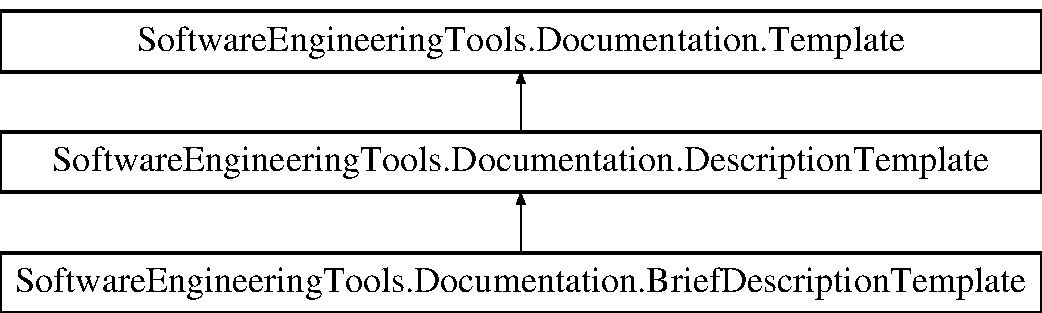
\includegraphics[height=3.000000cm]{class_software_engineering_tools_1_1_documentation_1_1_brief_description_template}
\end{center}
\end{figure}
\subsection*{Public Member Functions}
\begin{DoxyCompactItemize}
\item 
\hyperlink{class_software_engineering_tools_1_1_documentation_1_1_brief_description_template_a692c38875f55af387e592f5e6181d3ed}{Brief\+Description\+Template} (\hyperlink{class_software_engineering_tools_1_1_documentation_1_1_template}{Template} parent)
\item 
override void \hyperlink{class_software_engineering_tools_1_1_documentation_1_1_brief_description_template_a8e800971557ae734f89ac200352402ab}{Process} (\hyperlink{interface_software_engineering_tools_1_1_documentation_1_1_i_api_doc_template_processor}{I\+Api\+Doc\+Template\+Processor} processor)
\end{DoxyCompactItemize}
\subsection*{Additional Inherited Members}


\subsection{Detailed Description}


Definition at line 494 of file Api\+Doc\+Template.\+cs.



\subsection{Constructor \& Destructor Documentation}
\hypertarget{class_software_engineering_tools_1_1_documentation_1_1_brief_description_template_a692c38875f55af387e592f5e6181d3ed}{\index{Software\+Engineering\+Tools\+::\+Documentation\+::\+Brief\+Description\+Template@{Software\+Engineering\+Tools\+::\+Documentation\+::\+Brief\+Description\+Template}!Brief\+Description\+Template@{Brief\+Description\+Template}}
\index{Brief\+Description\+Template@{Brief\+Description\+Template}!Software\+Engineering\+Tools\+::\+Documentation\+::\+Brief\+Description\+Template@{Software\+Engineering\+Tools\+::\+Documentation\+::\+Brief\+Description\+Template}}
\subsubsection[{Brief\+Description\+Template}]{\setlength{\rightskip}{0pt plus 5cm}Software\+Engineering\+Tools.\+Documentation.\+Brief\+Description\+Template.\+Brief\+Description\+Template (
\begin{DoxyParamCaption}
\item[{{\bf Template}}]{parent}
\end{DoxyParamCaption}
)}}\label{class_software_engineering_tools_1_1_documentation_1_1_brief_description_template_a692c38875f55af387e592f5e6181d3ed}


Definition at line 496 of file Api\+Doc\+Template.\+cs.



\subsection{Member Function Documentation}
\hypertarget{class_software_engineering_tools_1_1_documentation_1_1_brief_description_template_a8e800971557ae734f89ac200352402ab}{\index{Software\+Engineering\+Tools\+::\+Documentation\+::\+Brief\+Description\+Template@{Software\+Engineering\+Tools\+::\+Documentation\+::\+Brief\+Description\+Template}!Process@{Process}}
\index{Process@{Process}!Software\+Engineering\+Tools\+::\+Documentation\+::\+Brief\+Description\+Template@{Software\+Engineering\+Tools\+::\+Documentation\+::\+Brief\+Description\+Template}}
\subsubsection[{Process}]{\setlength{\rightskip}{0pt plus 5cm}override void Software\+Engineering\+Tools.\+Documentation.\+Brief\+Description\+Template.\+Process (
\begin{DoxyParamCaption}
\item[{{\bf I\+Api\+Doc\+Template\+Processor}}]{processor}
\end{DoxyParamCaption}
)\hspace{0.3cm}{\ttfamily [virtual]}}}\label{class_software_engineering_tools_1_1_documentation_1_1_brief_description_template_a8e800971557ae734f89ac200352402ab}


Reimplemented from \hyperlink{class_software_engineering_tools_1_1_documentation_1_1_description_template_aacc8ff3057e26331de9f4f58ae0bc715}{Software\+Engineering\+Tools.\+Documentation.\+Description\+Template}.



Definition at line 502 of file Api\+Doc\+Template.\+cs.



The documentation for this class was generated from the following file\+:\begin{DoxyCompactItemize}
\item 
Api\+Doc\+Lib/\hyperlink{_api_doc_template_8cs}{Api\+Doc\+Template.\+cs}\end{DoxyCompactItemize}

\hypertarget{class_software_engineering_tools_1_1_documentation_1_1_classifier_list_template}{\section{Software\+Engineering\+Tools.\+Documentation.\+Classifier\+List\+Template Class Reference}
\label{class_software_engineering_tools_1_1_documentation_1_1_classifier_list_template}\index{Software\+Engineering\+Tools.\+Documentation.\+Classifier\+List\+Template@{Software\+Engineering\+Tools.\+Documentation.\+Classifier\+List\+Template}}
}
Inheritance diagram for Software\+Engineering\+Tools.\+Documentation.\+Classifier\+List\+Template\+:\begin{figure}[H]
\begin{center}
\leavevmode
\includegraphics[height=1.414141cm]{class_software_engineering_tools_1_1_documentation_1_1_classifier_list_template}
\end{center}
\end{figure}
\subsection*{Public Member Functions}
\begin{DoxyCompactItemize}
\item 
\hyperlink{class_software_engineering_tools_1_1_documentation_1_1_classifier_list_template_ab6d92fcf3c3f08dcda4a3136a23bbec1}{Classifier\+List\+Template} (\hyperlink{class_software_engineering_tools_1_1_documentation_1_1_template}{Template} parent)
\item 
override void \hyperlink{class_software_engineering_tools_1_1_documentation_1_1_classifier_list_template_a119ae8eeb938465c5aaf44780e2f8876}{Process} (\hyperlink{interface_software_engineering_tools_1_1_documentation_1_1_i_api_doc_template_processor}{I\+Api\+Doc\+Template\+Processor} processor)
\end{DoxyCompactItemize}
\subsection*{Additional Inherited Members}


\subsection{Detailed Description}


Definition at line 347 of file Api\+Doc\+Template.\+cs.



\subsection{Constructor \& Destructor Documentation}
\hypertarget{class_software_engineering_tools_1_1_documentation_1_1_classifier_list_template_ab6d92fcf3c3f08dcda4a3136a23bbec1}{\index{Software\+Engineering\+Tools\+::\+Documentation\+::\+Classifier\+List\+Template@{Software\+Engineering\+Tools\+::\+Documentation\+::\+Classifier\+List\+Template}!Classifier\+List\+Template@{Classifier\+List\+Template}}
\index{Classifier\+List\+Template@{Classifier\+List\+Template}!Software\+Engineering\+Tools\+::\+Documentation\+::\+Classifier\+List\+Template@{Software\+Engineering\+Tools\+::\+Documentation\+::\+Classifier\+List\+Template}}
\subsubsection[{Classifier\+List\+Template}]{\setlength{\rightskip}{0pt plus 5cm}Software\+Engineering\+Tools.\+Documentation.\+Classifier\+List\+Template.\+Classifier\+List\+Template (
\begin{DoxyParamCaption}
\item[{{\bf Template}}]{parent}
\end{DoxyParamCaption}
)}}\label{class_software_engineering_tools_1_1_documentation_1_1_classifier_list_template_ab6d92fcf3c3f08dcda4a3136a23bbec1}


Definition at line 349 of file Api\+Doc\+Template.\+cs.



\subsection{Member Function Documentation}
\hypertarget{class_software_engineering_tools_1_1_documentation_1_1_classifier_list_template_a119ae8eeb938465c5aaf44780e2f8876}{\index{Software\+Engineering\+Tools\+::\+Documentation\+::\+Classifier\+List\+Template@{Software\+Engineering\+Tools\+::\+Documentation\+::\+Classifier\+List\+Template}!Process@{Process}}
\index{Process@{Process}!Software\+Engineering\+Tools\+::\+Documentation\+::\+Classifier\+List\+Template@{Software\+Engineering\+Tools\+::\+Documentation\+::\+Classifier\+List\+Template}}
\subsubsection[{Process}]{\setlength{\rightskip}{0pt plus 5cm}override void Software\+Engineering\+Tools.\+Documentation.\+Classifier\+List\+Template.\+Process (
\begin{DoxyParamCaption}
\item[{{\bf I\+Api\+Doc\+Template\+Processor}}]{processor}
\end{DoxyParamCaption}
)\hspace{0.3cm}{\ttfamily [virtual]}}}\label{class_software_engineering_tools_1_1_documentation_1_1_classifier_list_template_a119ae8eeb938465c5aaf44780e2f8876}


Implements \hyperlink{class_software_engineering_tools_1_1_documentation_1_1_template_ab13b45a10b7eb65a0b6c15dbc1318664}{Software\+Engineering\+Tools.\+Documentation.\+Template}.



Reimplemented in \hyperlink{class_software_engineering_tools_1_1_documentation_1_1_enum_list_template_ab40ecbc15d3643dcd54cc7c4fdc7a42e}{Software\+Engineering\+Tools.\+Documentation.\+Enum\+List\+Template}, \hyperlink{class_software_engineering_tools_1_1_documentation_1_1_struct_list_template_ae89463eba79df4d331672e9774a65885}{Software\+Engineering\+Tools.\+Documentation.\+Struct\+List\+Template}, \hyperlink{class_software_engineering_tools_1_1_documentation_1_1_class_list_template_a310a651d73cc35f939bf302fd5233172}{Software\+Engineering\+Tools.\+Documentation.\+Class\+List\+Template}, and \hyperlink{class_software_engineering_tools_1_1_documentation_1_1_interface_list_template_a9c3f88c7e8e3444af953ccc3b926ee13}{Software\+Engineering\+Tools.\+Documentation.\+Interface\+List\+Template}.



Definition at line 354 of file Api\+Doc\+Template.\+cs.



The documentation for this class was generated from the following file\+:\begin{DoxyCompactItemize}
\item 
Api\+Doc\+Lib/\hyperlink{_api_doc_template_8cs}{Api\+Doc\+Template.\+cs}\end{DoxyCompactItemize}

\hypertarget{class_software_engineering_tools_1_1_documentation_1_1_class_list_template}{\section{Software\+Engineering\+Tools.\+Documentation.\+Class\+List\+Template Class Reference}
\label{class_software_engineering_tools_1_1_documentation_1_1_class_list_template}\index{Software\+Engineering\+Tools.\+Documentation.\+Class\+List\+Template@{Software\+Engineering\+Tools.\+Documentation.\+Class\+List\+Template}}
}
Inheritance diagram for Software\+Engineering\+Tools.\+Documentation.\+Class\+List\+Template\+:\begin{figure}[H]
\begin{center}
\leavevmode
\includegraphics[height=4.000000cm]{class_software_engineering_tools_1_1_documentation_1_1_class_list_template}
\end{center}
\end{figure}
\subsection*{Public Member Functions}
\begin{DoxyCompactItemize}
\item 
\hyperlink{class_software_engineering_tools_1_1_documentation_1_1_class_list_template_a722a03a1b38c55ff5bdb88abba363d6f}{Class\+List\+Template} (\hyperlink{class_software_engineering_tools_1_1_documentation_1_1_template}{Template} parent)
\item 
override void \hyperlink{class_software_engineering_tools_1_1_documentation_1_1_class_list_template_a310a651d73cc35f939bf302fd5233172}{Process} (\hyperlink{interface_software_engineering_tools_1_1_documentation_1_1_i_api_doc_template_processor}{I\+Api\+Doc\+Template\+Processor} processor)
\end{DoxyCompactItemize}
\subsection*{Additional Inherited Members}


\subsection{Detailed Description}


Definition at line 373 of file Api\+Doc\+Template.\+cs.



\subsection{Constructor \& Destructor Documentation}
\hypertarget{class_software_engineering_tools_1_1_documentation_1_1_class_list_template_a722a03a1b38c55ff5bdb88abba363d6f}{\index{Software\+Engineering\+Tools\+::\+Documentation\+::\+Class\+List\+Template@{Software\+Engineering\+Tools\+::\+Documentation\+::\+Class\+List\+Template}!Class\+List\+Template@{Class\+List\+Template}}
\index{Class\+List\+Template@{Class\+List\+Template}!Software\+Engineering\+Tools\+::\+Documentation\+::\+Class\+List\+Template@{Software\+Engineering\+Tools\+::\+Documentation\+::\+Class\+List\+Template}}
\subsubsection[{Class\+List\+Template}]{\setlength{\rightskip}{0pt plus 5cm}Software\+Engineering\+Tools.\+Documentation.\+Class\+List\+Template.\+Class\+List\+Template (
\begin{DoxyParamCaption}
\item[{{\bf Template}}]{parent}
\end{DoxyParamCaption}
)}}\label{class_software_engineering_tools_1_1_documentation_1_1_class_list_template_a722a03a1b38c55ff5bdb88abba363d6f}


Definition at line 375 of file Api\+Doc\+Template.\+cs.



\subsection{Member Function Documentation}
\hypertarget{class_software_engineering_tools_1_1_documentation_1_1_class_list_template_a310a651d73cc35f939bf302fd5233172}{\index{Software\+Engineering\+Tools\+::\+Documentation\+::\+Class\+List\+Template@{Software\+Engineering\+Tools\+::\+Documentation\+::\+Class\+List\+Template}!Process@{Process}}
\index{Process@{Process}!Software\+Engineering\+Tools\+::\+Documentation\+::\+Class\+List\+Template@{Software\+Engineering\+Tools\+::\+Documentation\+::\+Class\+List\+Template}}
\subsubsection[{Process}]{\setlength{\rightskip}{0pt plus 5cm}override void Software\+Engineering\+Tools.\+Documentation.\+Class\+List\+Template.\+Process (
\begin{DoxyParamCaption}
\item[{{\bf I\+Api\+Doc\+Template\+Processor}}]{processor}
\end{DoxyParamCaption}
)\hspace{0.3cm}{\ttfamily [virtual]}}}\label{class_software_engineering_tools_1_1_documentation_1_1_class_list_template_a310a651d73cc35f939bf302fd5233172}


Reimplemented from \hyperlink{class_software_engineering_tools_1_1_documentation_1_1_classifier_list_template_a119ae8eeb938465c5aaf44780e2f8876}{Software\+Engineering\+Tools.\+Documentation.\+Classifier\+List\+Template}.



Definition at line 380 of file Api\+Doc\+Template.\+cs.



The documentation for this class was generated from the following file\+:\begin{DoxyCompactItemize}
\item 
Api\+Doc\+Lib/\hyperlink{_api_doc_template_8cs}{Api\+Doc\+Template.\+cs}\end{DoxyCompactItemize}

\hypertarget{class_software_engineering_tools_1_1_documentation_1_1_compound}{\section{Software\+Engineering\+Tools.\+Documentation.\+Compound Class Reference}
\label{class_software_engineering_tools_1_1_documentation_1_1_compound}\index{Software\+Engineering\+Tools.\+Documentation.\+Compound@{Software\+Engineering\+Tools.\+Documentation.\+Compound}}
}
Inheritance diagram for Software\+Engineering\+Tools.\+Documentation.\+Compound\+:\begin{figure}[H]
\begin{center}
\leavevmode
\includegraphics[height=0.806916cm]{class_software_engineering_tools_1_1_documentation_1_1_compound}
\end{center}
\end{figure}
\subsection*{Public Member Functions}
\begin{DoxyCompactItemize}
\item 
\hyperlink{class_software_engineering_tools_1_1_documentation_1_1_compound_a4e7df725cc78a016399778b91e261bd0}{Compound} ()
\item 
override string \hyperlink{class_software_engineering_tools_1_1_documentation_1_1_compound_a2450d96253aafa7fd3384b67b1ab01d8}{To\+String} ()
\end{DoxyCompactItemize}
\subsection*{Properties}
\begin{DoxyCompactItemize}
\item 
string \hyperlink{class_software_engineering_tools_1_1_documentation_1_1_compound_a1394e3961d62b46fa478767c2b267776}{Identifier}\hspace{0.3cm}{\ttfamily  \mbox{[}get, set\mbox{]}}
\item 
string \hyperlink{class_software_engineering_tools_1_1_documentation_1_1_compound_ac03a88be9a7e7a11dd3c12006ae65879}{Name}\hspace{0.3cm}{\ttfamily  \mbox{[}get, set\mbox{]}}
\item 
string \hyperlink{class_software_engineering_tools_1_1_documentation_1_1_compound_a873e7d81cae2f4cb5c6cca41014cd02d}{Title}\hspace{0.3cm}{\ttfamily  \mbox{[}get, set\mbox{]}}
\item 
\hyperlink{namespace_software_engineering_tools_1_1_documentation_aae490e51e07ef6e5540a2f2c04fccbb1}{Compound\+Kind} \hyperlink{class_software_engineering_tools_1_1_documentation_1_1_compound_ae53780f3f48f262502a939871432292f}{Kind}\hspace{0.3cm}{\ttfamily  \mbox{[}get, set\mbox{]}}
\item 
\hyperlink{class_software_engineering_tools_1_1_documentation_1_1_description}{Description} \hyperlink{class_software_engineering_tools_1_1_documentation_1_1_compound_a4bfcfda760068c85256a0723b5ce1921}{Brief\+Description}\hspace{0.3cm}{\ttfamily  \mbox{[}get, set\mbox{]}}
\item 
\hyperlink{class_software_engineering_tools_1_1_documentation_1_1_description}{Description} \hyperlink{class_software_engineering_tools_1_1_documentation_1_1_compound_a77ca6711192dfb78bcd2f0b513e74b2e}{Description}\hspace{0.3cm}{\ttfamily  \mbox{[}get, set\mbox{]}}
\item 
\hyperlink{class_software_engineering_tools_1_1_documentation_1_1_dox_program_listing}{Dox\+Program\+Listing} \hyperlink{class_software_engineering_tools_1_1_documentation_1_1_compound_a6682b35f8afccbbecd77f504665b1cb7}{Program\+Listing}\hspace{0.3cm}{\ttfamily  \mbox{[}get, set\mbox{]}}
\item 
\hyperlink{class_software_engineering_tools_1_1_documentation_1_1_location}{Location} \hyperlink{class_software_engineering_tools_1_1_documentation_1_1_compound_ae491a737dd879c0665bd81a1273af091}{Location}\hspace{0.3cm}{\ttfamily  \mbox{[}get, set\mbox{]}}
\end{DoxyCompactItemize}


\subsection{Detailed Description}


Definition at line 98 of file Doxygen.\+cs.



\subsection{Constructor \& Destructor Documentation}
\hypertarget{class_software_engineering_tools_1_1_documentation_1_1_compound_a4e7df725cc78a016399778b91e261bd0}{\index{Software\+Engineering\+Tools\+::\+Documentation\+::\+Compound@{Software\+Engineering\+Tools\+::\+Documentation\+::\+Compound}!Compound@{Compound}}
\index{Compound@{Compound}!Software\+Engineering\+Tools\+::\+Documentation\+::\+Compound@{Software\+Engineering\+Tools\+::\+Documentation\+::\+Compound}}
\subsubsection[{Compound}]{\setlength{\rightskip}{0pt plus 5cm}Software\+Engineering\+Tools.\+Documentation.\+Compound.\+Compound (
\begin{DoxyParamCaption}
{}
\end{DoxyParamCaption}
)}}\label{class_software_engineering_tools_1_1_documentation_1_1_compound_a4e7df725cc78a016399778b91e261bd0}


Definition at line 109 of file Doxygen.\+cs.



\subsection{Member Function Documentation}
\hypertarget{class_software_engineering_tools_1_1_documentation_1_1_compound_a2450d96253aafa7fd3384b67b1ab01d8}{\index{Software\+Engineering\+Tools\+::\+Documentation\+::\+Compound@{Software\+Engineering\+Tools\+::\+Documentation\+::\+Compound}!To\+String@{To\+String}}
\index{To\+String@{To\+String}!Software\+Engineering\+Tools\+::\+Documentation\+::\+Compound@{Software\+Engineering\+Tools\+::\+Documentation\+::\+Compound}}
\subsubsection[{To\+String}]{\setlength{\rightskip}{0pt plus 5cm}override string Software\+Engineering\+Tools.\+Documentation.\+Compound.\+To\+String (
\begin{DoxyParamCaption}
{}
\end{DoxyParamCaption}
)}}\label{class_software_engineering_tools_1_1_documentation_1_1_compound_a2450d96253aafa7fd3384b67b1ab01d8}


Definition at line 113 of file Doxygen.\+cs.



\subsection{Property Documentation}
\hypertarget{class_software_engineering_tools_1_1_documentation_1_1_compound_a4bfcfda760068c85256a0723b5ce1921}{\index{Software\+Engineering\+Tools\+::\+Documentation\+::\+Compound@{Software\+Engineering\+Tools\+::\+Documentation\+::\+Compound}!Brief\+Description@{Brief\+Description}}
\index{Brief\+Description@{Brief\+Description}!Software\+Engineering\+Tools\+::\+Documentation\+::\+Compound@{Software\+Engineering\+Tools\+::\+Documentation\+::\+Compound}}
\subsubsection[{Brief\+Description}]{\setlength{\rightskip}{0pt plus 5cm}{\bf Description} Software\+Engineering\+Tools.\+Documentation.\+Compound.\+Brief\+Description\hspace{0.3cm}{\ttfamily [get]}, {\ttfamily [set]}}}\label{class_software_engineering_tools_1_1_documentation_1_1_compound_a4bfcfda760068c85256a0723b5ce1921}


Definition at line 104 of file Doxygen.\+cs.

\hypertarget{class_software_engineering_tools_1_1_documentation_1_1_compound_a77ca6711192dfb78bcd2f0b513e74b2e}{\index{Software\+Engineering\+Tools\+::\+Documentation\+::\+Compound@{Software\+Engineering\+Tools\+::\+Documentation\+::\+Compound}!Description@{Description}}
\index{Description@{Description}!Software\+Engineering\+Tools\+::\+Documentation\+::\+Compound@{Software\+Engineering\+Tools\+::\+Documentation\+::\+Compound}}
\subsubsection[{Description}]{\setlength{\rightskip}{0pt plus 5cm}{\bf Description} Software\+Engineering\+Tools.\+Documentation.\+Compound.\+Description\hspace{0.3cm}{\ttfamily [get]}, {\ttfamily [set]}}}\label{class_software_engineering_tools_1_1_documentation_1_1_compound_a77ca6711192dfb78bcd2f0b513e74b2e}


Definition at line 105 of file Doxygen.\+cs.

\hypertarget{class_software_engineering_tools_1_1_documentation_1_1_compound_a1394e3961d62b46fa478767c2b267776}{\index{Software\+Engineering\+Tools\+::\+Documentation\+::\+Compound@{Software\+Engineering\+Tools\+::\+Documentation\+::\+Compound}!Identifier@{Identifier}}
\index{Identifier@{Identifier}!Software\+Engineering\+Tools\+::\+Documentation\+::\+Compound@{Software\+Engineering\+Tools\+::\+Documentation\+::\+Compound}}
\subsubsection[{Identifier}]{\setlength{\rightskip}{0pt plus 5cm}string Software\+Engineering\+Tools.\+Documentation.\+Compound.\+Identifier\hspace{0.3cm}{\ttfamily [get]}, {\ttfamily [set]}}}\label{class_software_engineering_tools_1_1_documentation_1_1_compound_a1394e3961d62b46fa478767c2b267776}


Definition at line 100 of file Doxygen.\+cs.

\hypertarget{class_software_engineering_tools_1_1_documentation_1_1_compound_ae53780f3f48f262502a939871432292f}{\index{Software\+Engineering\+Tools\+::\+Documentation\+::\+Compound@{Software\+Engineering\+Tools\+::\+Documentation\+::\+Compound}!Kind@{Kind}}
\index{Kind@{Kind}!Software\+Engineering\+Tools\+::\+Documentation\+::\+Compound@{Software\+Engineering\+Tools\+::\+Documentation\+::\+Compound}}
\subsubsection[{Kind}]{\setlength{\rightskip}{0pt plus 5cm}{\bf Compound\+Kind} Software\+Engineering\+Tools.\+Documentation.\+Compound.\+Kind\hspace{0.3cm}{\ttfamily [get]}, {\ttfamily [set]}}}\label{class_software_engineering_tools_1_1_documentation_1_1_compound_ae53780f3f48f262502a939871432292f}


Definition at line 103 of file Doxygen.\+cs.

\hypertarget{class_software_engineering_tools_1_1_documentation_1_1_compound_ae491a737dd879c0665bd81a1273af091}{\index{Software\+Engineering\+Tools\+::\+Documentation\+::\+Compound@{Software\+Engineering\+Tools\+::\+Documentation\+::\+Compound}!Location@{Location}}
\index{Location@{Location}!Software\+Engineering\+Tools\+::\+Documentation\+::\+Compound@{Software\+Engineering\+Tools\+::\+Documentation\+::\+Compound}}
\subsubsection[{Location}]{\setlength{\rightskip}{0pt plus 5cm}{\bf Location} Software\+Engineering\+Tools.\+Documentation.\+Compound.\+Location\hspace{0.3cm}{\ttfamily [get]}, {\ttfamily [set]}}}\label{class_software_engineering_tools_1_1_documentation_1_1_compound_ae491a737dd879c0665bd81a1273af091}


Definition at line 107 of file Doxygen.\+cs.

\hypertarget{class_software_engineering_tools_1_1_documentation_1_1_compound_ac03a88be9a7e7a11dd3c12006ae65879}{\index{Software\+Engineering\+Tools\+::\+Documentation\+::\+Compound@{Software\+Engineering\+Tools\+::\+Documentation\+::\+Compound}!Name@{Name}}
\index{Name@{Name}!Software\+Engineering\+Tools\+::\+Documentation\+::\+Compound@{Software\+Engineering\+Tools\+::\+Documentation\+::\+Compound}}
\subsubsection[{Name}]{\setlength{\rightskip}{0pt plus 5cm}string Software\+Engineering\+Tools.\+Documentation.\+Compound.\+Name\hspace{0.3cm}{\ttfamily [get]}, {\ttfamily [set]}}}\label{class_software_engineering_tools_1_1_documentation_1_1_compound_ac03a88be9a7e7a11dd3c12006ae65879}


Definition at line 101 of file Doxygen.\+cs.

\hypertarget{class_software_engineering_tools_1_1_documentation_1_1_compound_a6682b35f8afccbbecd77f504665b1cb7}{\index{Software\+Engineering\+Tools\+::\+Documentation\+::\+Compound@{Software\+Engineering\+Tools\+::\+Documentation\+::\+Compound}!Program\+Listing@{Program\+Listing}}
\index{Program\+Listing@{Program\+Listing}!Software\+Engineering\+Tools\+::\+Documentation\+::\+Compound@{Software\+Engineering\+Tools\+::\+Documentation\+::\+Compound}}
\subsubsection[{Program\+Listing}]{\setlength{\rightskip}{0pt plus 5cm}{\bf Dox\+Program\+Listing} Software\+Engineering\+Tools.\+Documentation.\+Compound.\+Program\+Listing\hspace{0.3cm}{\ttfamily [get]}, {\ttfamily [set]}}}\label{class_software_engineering_tools_1_1_documentation_1_1_compound_a6682b35f8afccbbecd77f504665b1cb7}


Definition at line 106 of file Doxygen.\+cs.

\hypertarget{class_software_engineering_tools_1_1_documentation_1_1_compound_a873e7d81cae2f4cb5c6cca41014cd02d}{\index{Software\+Engineering\+Tools\+::\+Documentation\+::\+Compound@{Software\+Engineering\+Tools\+::\+Documentation\+::\+Compound}!Title@{Title}}
\index{Title@{Title}!Software\+Engineering\+Tools\+::\+Documentation\+::\+Compound@{Software\+Engineering\+Tools\+::\+Documentation\+::\+Compound}}
\subsubsection[{Title}]{\setlength{\rightskip}{0pt plus 5cm}string Software\+Engineering\+Tools.\+Documentation.\+Compound.\+Title\hspace{0.3cm}{\ttfamily [get]}, {\ttfamily [set]}}}\label{class_software_engineering_tools_1_1_documentation_1_1_compound_a873e7d81cae2f4cb5c6cca41014cd02d}


Definition at line 102 of file Doxygen.\+cs.



The documentation for this class was generated from the following file\+:\begin{DoxyCompactItemize}
\item 
Api\+Doc\+Lib/\hyperlink{_doxygen_8cs}{Doxygen.\+cs}\end{DoxyCompactItemize}

\hypertarget{class_software_engineering_tools_1_1_documentation_1_1_compound_index}{\section{Software\+Engineering\+Tools.\+Documentation.\+Compound\+Index Class Reference}
\label{class_software_engineering_tools_1_1_documentation_1_1_compound_index}\index{Software\+Engineering\+Tools.\+Documentation.\+Compound\+Index@{Software\+Engineering\+Tools.\+Documentation.\+Compound\+Index}}
}
\subsection*{Public Member Functions}
\begin{DoxyCompactItemize}
\item 
\hyperlink{class_software_engineering_tools_1_1_documentation_1_1_compound_index_ae91f253c49b676581d40cbd52f1644e0}{Compound\+Index} ()
\end{DoxyCompactItemize}
\subsection*{Properties}
\begin{DoxyCompactItemize}
\item 
string \hyperlink{class_software_engineering_tools_1_1_documentation_1_1_compound_index_a988308311c455fcb89b4b14545300752}{Identifier}\hspace{0.3cm}{\ttfamily  \mbox{[}get, set\mbox{]}}
\item 
string \hyperlink{class_software_engineering_tools_1_1_documentation_1_1_compound_index_af6581fddcc01a475db082ad5ef186d23}{Name}\hspace{0.3cm}{\ttfamily  \mbox{[}get, set\mbox{]}}
\item 
\hyperlink{namespace_software_engineering_tools_1_1_documentation_aae490e51e07ef6e5540a2f2c04fccbb1}{Compound\+Kind} \hyperlink{class_software_engineering_tools_1_1_documentation_1_1_compound_index_ab39d7c9817b5bc97122b11bc6ad84ab4}{Kind}\hspace{0.3cm}{\ttfamily  \mbox{[}get, set\mbox{]}}
\item 
\hyperlink{namespace_software_engineering_tools_1_1_documentation_ae0bccf4f49a76db084c1c316e5954ec9a4ee29ca12c7d126654bd0e5275de6135}{List}$<$ \hyperlink{class_software_engineering_tools_1_1_documentation_1_1_member_index}{Member\+Index} $>$ \hyperlink{class_software_engineering_tools_1_1_documentation_1_1_compound_index_a7010d81af3c92ae3595c88c89dc0cd49}{Members}\hspace{0.3cm}{\ttfamily  \mbox{[}get, set\mbox{]}}
\item 
\hyperlink{class_software_engineering_tools_1_1_documentation_1_1_compound}{Compound} \hyperlink{class_software_engineering_tools_1_1_documentation_1_1_compound_index_a2e6e9b608ac76ec7450c37d64017efa2}{Compound}\hspace{0.3cm}{\ttfamily  \mbox{[}get, set\mbox{]}}
\end{DoxyCompactItemize}


\subsection{Detailed Description}


Definition at line 22 of file Doxygen.\+cs.



\subsection{Constructor \& Destructor Documentation}
\hypertarget{class_software_engineering_tools_1_1_documentation_1_1_compound_index_ae91f253c49b676581d40cbd52f1644e0}{\index{Software\+Engineering\+Tools\+::\+Documentation\+::\+Compound\+Index@{Software\+Engineering\+Tools\+::\+Documentation\+::\+Compound\+Index}!Compound\+Index@{Compound\+Index}}
\index{Compound\+Index@{Compound\+Index}!Software\+Engineering\+Tools\+::\+Documentation\+::\+Compound\+Index@{Software\+Engineering\+Tools\+::\+Documentation\+::\+Compound\+Index}}
\subsubsection[{Compound\+Index}]{\setlength{\rightskip}{0pt plus 5cm}Software\+Engineering\+Tools.\+Documentation.\+Compound\+Index.\+Compound\+Index (
\begin{DoxyParamCaption}
{}
\end{DoxyParamCaption}
)}}\label{class_software_engineering_tools_1_1_documentation_1_1_compound_index_ae91f253c49b676581d40cbd52f1644e0}


Definition at line 29 of file Doxygen.\+cs.



\subsection{Property Documentation}
\hypertarget{class_software_engineering_tools_1_1_documentation_1_1_compound_index_a2e6e9b608ac76ec7450c37d64017efa2}{\index{Software\+Engineering\+Tools\+::\+Documentation\+::\+Compound\+Index@{Software\+Engineering\+Tools\+::\+Documentation\+::\+Compound\+Index}!Compound@{Compound}}
\index{Compound@{Compound}!Software\+Engineering\+Tools\+::\+Documentation\+::\+Compound\+Index@{Software\+Engineering\+Tools\+::\+Documentation\+::\+Compound\+Index}}
\subsubsection[{Compound}]{\setlength{\rightskip}{0pt plus 5cm}{\bf Compound} Software\+Engineering\+Tools.\+Documentation.\+Compound\+Index.\+Compound\hspace{0.3cm}{\ttfamily [get]}, {\ttfamily [set]}}}\label{class_software_engineering_tools_1_1_documentation_1_1_compound_index_a2e6e9b608ac76ec7450c37d64017efa2}


Definition at line 28 of file Doxygen.\+cs.

\hypertarget{class_software_engineering_tools_1_1_documentation_1_1_compound_index_a988308311c455fcb89b4b14545300752}{\index{Software\+Engineering\+Tools\+::\+Documentation\+::\+Compound\+Index@{Software\+Engineering\+Tools\+::\+Documentation\+::\+Compound\+Index}!Identifier@{Identifier}}
\index{Identifier@{Identifier}!Software\+Engineering\+Tools\+::\+Documentation\+::\+Compound\+Index@{Software\+Engineering\+Tools\+::\+Documentation\+::\+Compound\+Index}}
\subsubsection[{Identifier}]{\setlength{\rightskip}{0pt plus 5cm}string Software\+Engineering\+Tools.\+Documentation.\+Compound\+Index.\+Identifier\hspace{0.3cm}{\ttfamily [get]}, {\ttfamily [set]}}}\label{class_software_engineering_tools_1_1_documentation_1_1_compound_index_a988308311c455fcb89b4b14545300752}


Definition at line 24 of file Doxygen.\+cs.

\hypertarget{class_software_engineering_tools_1_1_documentation_1_1_compound_index_ab39d7c9817b5bc97122b11bc6ad84ab4}{\index{Software\+Engineering\+Tools\+::\+Documentation\+::\+Compound\+Index@{Software\+Engineering\+Tools\+::\+Documentation\+::\+Compound\+Index}!Kind@{Kind}}
\index{Kind@{Kind}!Software\+Engineering\+Tools\+::\+Documentation\+::\+Compound\+Index@{Software\+Engineering\+Tools\+::\+Documentation\+::\+Compound\+Index}}
\subsubsection[{Kind}]{\setlength{\rightskip}{0pt plus 5cm}{\bf Compound\+Kind} Software\+Engineering\+Tools.\+Documentation.\+Compound\+Index.\+Kind\hspace{0.3cm}{\ttfamily [get]}, {\ttfamily [set]}}}\label{class_software_engineering_tools_1_1_documentation_1_1_compound_index_ab39d7c9817b5bc97122b11bc6ad84ab4}


Definition at line 26 of file Doxygen.\+cs.

\hypertarget{class_software_engineering_tools_1_1_documentation_1_1_compound_index_a7010d81af3c92ae3595c88c89dc0cd49}{\index{Software\+Engineering\+Tools\+::\+Documentation\+::\+Compound\+Index@{Software\+Engineering\+Tools\+::\+Documentation\+::\+Compound\+Index}!Members@{Members}}
\index{Members@{Members}!Software\+Engineering\+Tools\+::\+Documentation\+::\+Compound\+Index@{Software\+Engineering\+Tools\+::\+Documentation\+::\+Compound\+Index}}
\subsubsection[{Members}]{\setlength{\rightskip}{0pt plus 5cm}{\bf List}$<${\bf Member\+Index}$>$ Software\+Engineering\+Tools.\+Documentation.\+Compound\+Index.\+Members\hspace{0.3cm}{\ttfamily [get]}, {\ttfamily [set]}}}\label{class_software_engineering_tools_1_1_documentation_1_1_compound_index_a7010d81af3c92ae3595c88c89dc0cd49}


Definition at line 27 of file Doxygen.\+cs.

\hypertarget{class_software_engineering_tools_1_1_documentation_1_1_compound_index_af6581fddcc01a475db082ad5ef186d23}{\index{Software\+Engineering\+Tools\+::\+Documentation\+::\+Compound\+Index@{Software\+Engineering\+Tools\+::\+Documentation\+::\+Compound\+Index}!Name@{Name}}
\index{Name@{Name}!Software\+Engineering\+Tools\+::\+Documentation\+::\+Compound\+Index@{Software\+Engineering\+Tools\+::\+Documentation\+::\+Compound\+Index}}
\subsubsection[{Name}]{\setlength{\rightskip}{0pt plus 5cm}string Software\+Engineering\+Tools.\+Documentation.\+Compound\+Index.\+Name\hspace{0.3cm}{\ttfamily [get]}, {\ttfamily [set]}}}\label{class_software_engineering_tools_1_1_documentation_1_1_compound_index_af6581fddcc01a475db082ad5ef186d23}


Definition at line 25 of file Doxygen.\+cs.



The documentation for this class was generated from the following file\+:\begin{DoxyCompactItemize}
\item 
Api\+Doc\+Lib/\hyperlink{_doxygen_8cs}{Doxygen.\+cs}\end{DoxyCompactItemize}

\hypertarget{class_software_engineering_tools_1_1_documentation_1_1_description}{\section{Software\+Engineering\+Tools.\+Documentation.\+Description Class Reference}
\label{class_software_engineering_tools_1_1_documentation_1_1_description}\index{Software\+Engineering\+Tools.\+Documentation.\+Description@{Software\+Engineering\+Tools.\+Documentation.\+Description}}
}
Inheritance diagram for Software\+Engineering\+Tools.\+Documentation.\+Description\+:\begin{figure}[H]
\begin{center}
\leavevmode
\includegraphics[height=4.000000cm]{class_software_engineering_tools_1_1_documentation_1_1_description}
\end{center}
\end{figure}
\subsection*{Public Member Functions}
\begin{DoxyCompactItemize}
\item 
\hyperlink{class_software_engineering_tools_1_1_documentation_1_1_description_af6858f1c08f3411ed90e344ba0eac0bd}{Description} ()
\end{DoxyCompactItemize}
\subsection*{Properties}
\begin{DoxyCompactItemize}
\item 
string \hyperlink{class_software_engineering_tools_1_1_documentation_1_1_description_a037f99f3a2542aac9a84a820934c3134}{Title}\hspace{0.3cm}{\ttfamily  \mbox{[}get, set\mbox{]}}
\item 
\hyperlink{namespace_software_engineering_tools_1_1_documentation_ae0bccf4f49a76db084c1c316e5954ec9a4ee29ca12c7d126654bd0e5275de6135}{List}$<$ \hyperlink{class_software_engineering_tools_1_1_documentation_1_1_doc_para}{Doc\+Para} $>$ \hyperlink{class_software_engineering_tools_1_1_documentation_1_1_description_aac9bd87b495aeecf95fe6b696f929cae}{Paragraphs}\hspace{0.3cm}{\ttfamily  \mbox{[}get, set\mbox{]}}
\item 
\hyperlink{namespace_software_engineering_tools_1_1_documentation_ae0bccf4f49a76db084c1c316e5954ec9a4ee29ca12c7d126654bd0e5275de6135}{List}$<$ \hyperlink{class_software_engineering_tools_1_1_documentation_1_1_doc_sect}{Doc\+Sect} $>$ \hyperlink{class_software_engineering_tools_1_1_documentation_1_1_description_a77b76a6eb0dde987ea3b919ccd094a25}{Sections}\hspace{0.3cm}{\ttfamily  \mbox{[}get, set\mbox{]}}
\item 
\hyperlink{class_software_engineering_tools_1_1_documentation_1_1_description}{Description} \hyperlink{class_software_engineering_tools_1_1_documentation_1_1_description_a26bb938e6775c1c7bfeff9ffd6f913f7}{Internal}\hspace{0.3cm}{\ttfamily  \mbox{[}get, set\mbox{]}}
\end{DoxyCompactItemize}


\subsection{Detailed Description}


Definition at line 440 of file Doxygen.\+cs.



\subsection{Constructor \& Destructor Documentation}
\hypertarget{class_software_engineering_tools_1_1_documentation_1_1_description_af6858f1c08f3411ed90e344ba0eac0bd}{\index{Software\+Engineering\+Tools\+::\+Documentation\+::\+Description@{Software\+Engineering\+Tools\+::\+Documentation\+::\+Description}!Description@{Description}}
\index{Description@{Description}!Software\+Engineering\+Tools\+::\+Documentation\+::\+Description@{Software\+Engineering\+Tools\+::\+Documentation\+::\+Description}}
\subsubsection[{Description}]{\setlength{\rightskip}{0pt plus 5cm}Software\+Engineering\+Tools.\+Documentation.\+Description.\+Description (
\begin{DoxyParamCaption}
{}
\end{DoxyParamCaption}
)}}\label{class_software_engineering_tools_1_1_documentation_1_1_description_af6858f1c08f3411ed90e344ba0eac0bd}


Definition at line 447 of file Doxygen.\+cs.



\subsection{Property Documentation}
\hypertarget{class_software_engineering_tools_1_1_documentation_1_1_description_a26bb938e6775c1c7bfeff9ffd6f913f7}{\index{Software\+Engineering\+Tools\+::\+Documentation\+::\+Description@{Software\+Engineering\+Tools\+::\+Documentation\+::\+Description}!Internal@{Internal}}
\index{Internal@{Internal}!Software\+Engineering\+Tools\+::\+Documentation\+::\+Description@{Software\+Engineering\+Tools\+::\+Documentation\+::\+Description}}
\subsubsection[{Internal}]{\setlength{\rightskip}{0pt plus 5cm}{\bf Description} Software\+Engineering\+Tools.\+Documentation.\+Description.\+Internal\hspace{0.3cm}{\ttfamily [get]}, {\ttfamily [set]}}}\label{class_software_engineering_tools_1_1_documentation_1_1_description_a26bb938e6775c1c7bfeff9ffd6f913f7}


Definition at line 445 of file Doxygen.\+cs.

\hypertarget{class_software_engineering_tools_1_1_documentation_1_1_description_aac9bd87b495aeecf95fe6b696f929cae}{\index{Software\+Engineering\+Tools\+::\+Documentation\+::\+Description@{Software\+Engineering\+Tools\+::\+Documentation\+::\+Description}!Paragraphs@{Paragraphs}}
\index{Paragraphs@{Paragraphs}!Software\+Engineering\+Tools\+::\+Documentation\+::\+Description@{Software\+Engineering\+Tools\+::\+Documentation\+::\+Description}}
\subsubsection[{Paragraphs}]{\setlength{\rightskip}{0pt plus 5cm}{\bf List}$<${\bf Doc\+Para}$>$ Software\+Engineering\+Tools.\+Documentation.\+Description.\+Paragraphs\hspace{0.3cm}{\ttfamily [get]}, {\ttfamily [set]}}}\label{class_software_engineering_tools_1_1_documentation_1_1_description_aac9bd87b495aeecf95fe6b696f929cae}


Definition at line 443 of file Doxygen.\+cs.

\hypertarget{class_software_engineering_tools_1_1_documentation_1_1_description_a77b76a6eb0dde987ea3b919ccd094a25}{\index{Software\+Engineering\+Tools\+::\+Documentation\+::\+Description@{Software\+Engineering\+Tools\+::\+Documentation\+::\+Description}!Sections@{Sections}}
\index{Sections@{Sections}!Software\+Engineering\+Tools\+::\+Documentation\+::\+Description@{Software\+Engineering\+Tools\+::\+Documentation\+::\+Description}}
\subsubsection[{Sections}]{\setlength{\rightskip}{0pt plus 5cm}{\bf List}$<${\bf Doc\+Sect}$>$ Software\+Engineering\+Tools.\+Documentation.\+Description.\+Sections\hspace{0.3cm}{\ttfamily [get]}, {\ttfamily [set]}}}\label{class_software_engineering_tools_1_1_documentation_1_1_description_a77b76a6eb0dde987ea3b919ccd094a25}


Definition at line 444 of file Doxygen.\+cs.

\hypertarget{class_software_engineering_tools_1_1_documentation_1_1_description_a037f99f3a2542aac9a84a820934c3134}{\index{Software\+Engineering\+Tools\+::\+Documentation\+::\+Description@{Software\+Engineering\+Tools\+::\+Documentation\+::\+Description}!Title@{Title}}
\index{Title@{Title}!Software\+Engineering\+Tools\+::\+Documentation\+::\+Description@{Software\+Engineering\+Tools\+::\+Documentation\+::\+Description}}
\subsubsection[{Title}]{\setlength{\rightskip}{0pt plus 5cm}string Software\+Engineering\+Tools.\+Documentation.\+Description.\+Title\hspace{0.3cm}{\ttfamily [get]}, {\ttfamily [set]}}}\label{class_software_engineering_tools_1_1_documentation_1_1_description_a037f99f3a2542aac9a84a820934c3134}


Definition at line 442 of file Doxygen.\+cs.



The documentation for this class was generated from the following file\+:\begin{DoxyCompactItemize}
\item 
Api\+Doc\+Lib/\hyperlink{_doxygen_8cs}{Doxygen.\+cs}\end{DoxyCompactItemize}

\hypertarget{class_software_engineering_tools_1_1_documentation_1_1_description_template}{\section{Software\+Engineering\+Tools.\+Documentation.\+Description\+Template Class Reference}
\label{class_software_engineering_tools_1_1_documentation_1_1_description_template}\index{Software\+Engineering\+Tools.\+Documentation.\+Description\+Template@{Software\+Engineering\+Tools.\+Documentation.\+Description\+Template}}
}
Inheritance diagram for Software\+Engineering\+Tools.\+Documentation.\+Description\+Template\+:\begin{figure}[H]
\begin{center}
\leavevmode
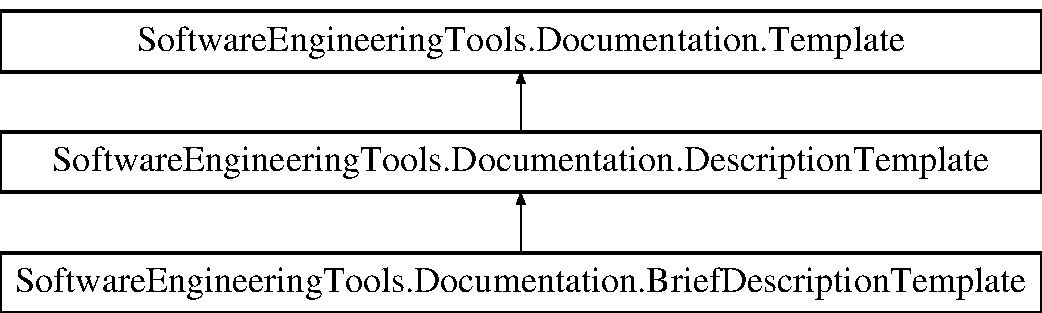
\includegraphics[height=3.000000cm]{class_software_engineering_tools_1_1_documentation_1_1_description_template}
\end{center}
\end{figure}
\subsection*{Public Member Functions}
\begin{DoxyCompactItemize}
\item 
\hyperlink{class_software_engineering_tools_1_1_documentation_1_1_description_template_aaf0d52969f8972fec61e23f8d41871e8}{Description\+Template} (\hyperlink{class_software_engineering_tools_1_1_documentation_1_1_template}{Template} parent)
\item 
override void \hyperlink{class_software_engineering_tools_1_1_documentation_1_1_description_template_aacc8ff3057e26331de9f4f58ae0bc715}{Process} (\hyperlink{interface_software_engineering_tools_1_1_documentation_1_1_i_api_doc_template_processor}{I\+Api\+Doc\+Template\+Processor} processor)
\end{DoxyCompactItemize}
\subsection*{Additional Inherited Members}


\subsection{Detailed Description}


Definition at line 480 of file Api\+Doc\+Template.\+cs.



\subsection{Constructor \& Destructor Documentation}
\hypertarget{class_software_engineering_tools_1_1_documentation_1_1_description_template_aaf0d52969f8972fec61e23f8d41871e8}{\index{Software\+Engineering\+Tools\+::\+Documentation\+::\+Description\+Template@{Software\+Engineering\+Tools\+::\+Documentation\+::\+Description\+Template}!Description\+Template@{Description\+Template}}
\index{Description\+Template@{Description\+Template}!Software\+Engineering\+Tools\+::\+Documentation\+::\+Description\+Template@{Software\+Engineering\+Tools\+::\+Documentation\+::\+Description\+Template}}
\subsubsection[{Description\+Template}]{\setlength{\rightskip}{0pt plus 5cm}Software\+Engineering\+Tools.\+Documentation.\+Description\+Template.\+Description\+Template (
\begin{DoxyParamCaption}
\item[{{\bf Template}}]{parent}
\end{DoxyParamCaption}
)}}\label{class_software_engineering_tools_1_1_documentation_1_1_description_template_aaf0d52969f8972fec61e23f8d41871e8}


Definition at line 482 of file Api\+Doc\+Template.\+cs.



\subsection{Member Function Documentation}
\hypertarget{class_software_engineering_tools_1_1_documentation_1_1_description_template_aacc8ff3057e26331de9f4f58ae0bc715}{\index{Software\+Engineering\+Tools\+::\+Documentation\+::\+Description\+Template@{Software\+Engineering\+Tools\+::\+Documentation\+::\+Description\+Template}!Process@{Process}}
\index{Process@{Process}!Software\+Engineering\+Tools\+::\+Documentation\+::\+Description\+Template@{Software\+Engineering\+Tools\+::\+Documentation\+::\+Description\+Template}}
\subsubsection[{Process}]{\setlength{\rightskip}{0pt plus 5cm}override void Software\+Engineering\+Tools.\+Documentation.\+Description\+Template.\+Process (
\begin{DoxyParamCaption}
\item[{{\bf I\+Api\+Doc\+Template\+Processor}}]{processor}
\end{DoxyParamCaption}
)\hspace{0.3cm}{\ttfamily [virtual]}}}\label{class_software_engineering_tools_1_1_documentation_1_1_description_template_aacc8ff3057e26331de9f4f58ae0bc715}


Implements \hyperlink{class_software_engineering_tools_1_1_documentation_1_1_template_ab13b45a10b7eb65a0b6c15dbc1318664}{Software\+Engineering\+Tools.\+Documentation.\+Template}.



Reimplemented in \hyperlink{class_software_engineering_tools_1_1_documentation_1_1_brief_description_template_a8e800971557ae734f89ac200352402ab}{Software\+Engineering\+Tools.\+Documentation.\+Brief\+Description\+Template}.



Definition at line 488 of file Api\+Doc\+Template.\+cs.



The documentation for this class was generated from the following file\+:\begin{DoxyCompactItemize}
\item 
Api\+Doc\+Lib/\hyperlink{_api_doc_template_8cs}{Api\+Doc\+Template.\+cs}\end{DoxyCompactItemize}

\hypertarget{class_software_engineering_tools_1_1_documentation_1_1_doc_anchor}{\section{Software\+Engineering\+Tools.\+Documentation.\+Doc\+Anchor Class Reference}
\label{class_software_engineering_tools_1_1_documentation_1_1_doc_anchor}\index{Software\+Engineering\+Tools.\+Documentation.\+Doc\+Anchor@{Software\+Engineering\+Tools.\+Documentation.\+Doc\+Anchor}}
}
Inheritance diagram for Software\+Engineering\+Tools.\+Documentation.\+Doc\+Anchor\+:\begin{figure}[H]
\begin{center}
\leavevmode
\includegraphics[height=3.000000cm]{class_software_engineering_tools_1_1_documentation_1_1_doc_anchor}
\end{center}
\end{figure}
\subsection*{Public Member Functions}
\begin{DoxyCompactItemize}
\item 
\hyperlink{class_software_engineering_tools_1_1_documentation_1_1_doc_anchor_aceb07534634cd6613fbd0dfc04d857a4}{Doc\+Anchor} ()
\end{DoxyCompactItemize}
\subsection*{Properties}
\begin{DoxyCompactItemize}
\item 
string \hyperlink{class_software_engineering_tools_1_1_documentation_1_1_doc_anchor_a8fdb6ce785bba95e544fb8a4da679395}{Id}\hspace{0.3cm}{\ttfamily  \mbox{[}get, set\mbox{]}}
\end{DoxyCompactItemize}


\subsection{Detailed Description}


Definition at line 716 of file Doxygen.\+cs.



\subsection{Constructor \& Destructor Documentation}
\hypertarget{class_software_engineering_tools_1_1_documentation_1_1_doc_anchor_aceb07534634cd6613fbd0dfc04d857a4}{\index{Software\+Engineering\+Tools\+::\+Documentation\+::\+Doc\+Anchor@{Software\+Engineering\+Tools\+::\+Documentation\+::\+Doc\+Anchor}!Doc\+Anchor@{Doc\+Anchor}}
\index{Doc\+Anchor@{Doc\+Anchor}!Software\+Engineering\+Tools\+::\+Documentation\+::\+Doc\+Anchor@{Software\+Engineering\+Tools\+::\+Documentation\+::\+Doc\+Anchor}}
\subsubsection[{Doc\+Anchor}]{\setlength{\rightskip}{0pt plus 5cm}Software\+Engineering\+Tools.\+Documentation.\+Doc\+Anchor.\+Doc\+Anchor (
\begin{DoxyParamCaption}
{}
\end{DoxyParamCaption}
)}}\label{class_software_engineering_tools_1_1_documentation_1_1_doc_anchor_aceb07534634cd6613fbd0dfc04d857a4}


Definition at line 720 of file Doxygen.\+cs.



\subsection{Property Documentation}
\hypertarget{class_software_engineering_tools_1_1_documentation_1_1_doc_anchor_a8fdb6ce785bba95e544fb8a4da679395}{\index{Software\+Engineering\+Tools\+::\+Documentation\+::\+Doc\+Anchor@{Software\+Engineering\+Tools\+::\+Documentation\+::\+Doc\+Anchor}!Id@{Id}}
\index{Id@{Id}!Software\+Engineering\+Tools\+::\+Documentation\+::\+Doc\+Anchor@{Software\+Engineering\+Tools\+::\+Documentation\+::\+Doc\+Anchor}}
\subsubsection[{Id}]{\setlength{\rightskip}{0pt plus 5cm}string Software\+Engineering\+Tools.\+Documentation.\+Doc\+Anchor.\+Id\hspace{0.3cm}{\ttfamily [get]}, {\ttfamily [set]}}}\label{class_software_engineering_tools_1_1_documentation_1_1_doc_anchor_a8fdb6ce785bba95e544fb8a4da679395}


Definition at line 718 of file Doxygen.\+cs.



The documentation for this class was generated from the following file\+:\begin{DoxyCompactItemize}
\item 
Api\+Doc\+Lib/\hyperlink{_doxygen_8cs}{Doxygen.\+cs}\end{DoxyCompactItemize}

\hypertarget{class_software_engineering_tools_1_1_documentation_1_1_doc_block_quote}{\section{Software\+Engineering\+Tools.\+Documentation.\+Doc\+Block\+Quote Class Reference}
\label{class_software_engineering_tools_1_1_documentation_1_1_doc_block_quote}\index{Software\+Engineering\+Tools.\+Documentation.\+Doc\+Block\+Quote@{Software\+Engineering\+Tools.\+Documentation.\+Doc\+Block\+Quote}}
}
Inheritance diagram for Software\+Engineering\+Tools.\+Documentation.\+Doc\+Block\+Quote\+:\begin{figure}[H]
\begin{center}
\leavevmode
\includegraphics[height=3.000000cm]{class_software_engineering_tools_1_1_documentation_1_1_doc_block_quote}
\end{center}
\end{figure}
\subsection*{Public Member Functions}
\begin{DoxyCompactItemize}
\item 
\hyperlink{class_software_engineering_tools_1_1_documentation_1_1_doc_block_quote_ac44ac51db0231efd5242390f082416de}{Doc\+Block\+Quote} ()
\end{DoxyCompactItemize}
\subsection*{Additional Inherited Members}


\subsection{Detailed Description}


Definition at line 1038 of file Doxygen.\+cs.



\subsection{Constructor \& Destructor Documentation}
\hypertarget{class_software_engineering_tools_1_1_documentation_1_1_doc_block_quote_ac44ac51db0231efd5242390f082416de}{\index{Software\+Engineering\+Tools\+::\+Documentation\+::\+Doc\+Block\+Quote@{Software\+Engineering\+Tools\+::\+Documentation\+::\+Doc\+Block\+Quote}!Doc\+Block\+Quote@{Doc\+Block\+Quote}}
\index{Doc\+Block\+Quote@{Doc\+Block\+Quote}!Software\+Engineering\+Tools\+::\+Documentation\+::\+Doc\+Block\+Quote@{Software\+Engineering\+Tools\+::\+Documentation\+::\+Doc\+Block\+Quote}}
\subsubsection[{Doc\+Block\+Quote}]{\setlength{\rightskip}{0pt plus 5cm}Software\+Engineering\+Tools.\+Documentation.\+Doc\+Block\+Quote.\+Doc\+Block\+Quote (
\begin{DoxyParamCaption}
{}
\end{DoxyParamCaption}
)}}\label{class_software_engineering_tools_1_1_documentation_1_1_doc_block_quote_ac44ac51db0231efd5242390f082416de}


Definition at line 1040 of file Doxygen.\+cs.



The documentation for this class was generated from the following file\+:\begin{DoxyCompactItemize}
\item 
Api\+Doc\+Lib/\hyperlink{_doxygen_8cs}{Doxygen.\+cs}\end{DoxyCompactItemize}

\hypertarget{class_software_engineering_tools_1_1_documentation_1_1_doc_caption}{\section{Software\+Engineering\+Tools.\+Documentation.\+Doc\+Caption Class Reference}
\label{class_software_engineering_tools_1_1_documentation_1_1_doc_caption}\index{Software\+Engineering\+Tools.\+Documentation.\+Doc\+Caption@{Software\+Engineering\+Tools.\+Documentation.\+Doc\+Caption}}
}
Inheritance diagram for Software\+Engineering\+Tools.\+Documentation.\+Doc\+Caption\+:\begin{figure}[H]
\begin{center}
\leavevmode
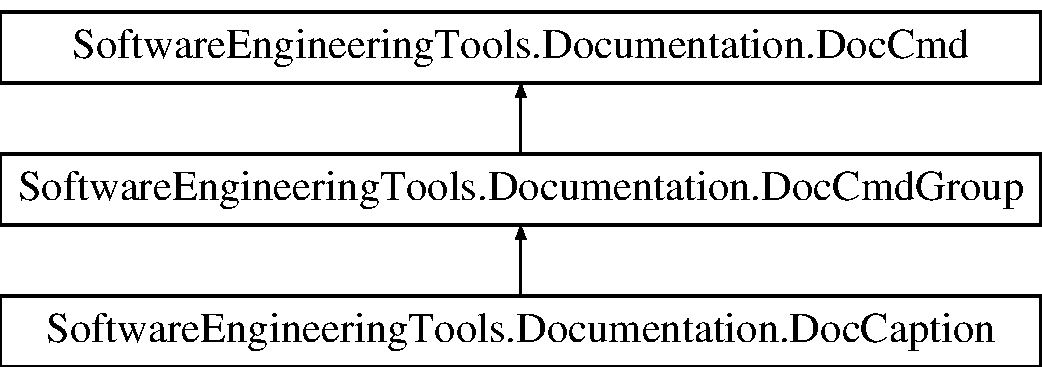
\includegraphics[height=3.000000cm]{class_software_engineering_tools_1_1_documentation_1_1_doc_caption}
\end{center}
\end{figure}
\subsection*{Public Member Functions}
\begin{DoxyCompactItemize}
\item 
\hyperlink{class_software_engineering_tools_1_1_documentation_1_1_doc_caption_a023a86d07d2247e1136007aad4e0c523}{Doc\+Caption} ()
\end{DoxyCompactItemize}
\subsection*{Additional Inherited Members}


\subsection{Detailed Description}


Definition at line 836 of file Doxygen.\+cs.



\subsection{Constructor \& Destructor Documentation}
\hypertarget{class_software_engineering_tools_1_1_documentation_1_1_doc_caption_a023a86d07d2247e1136007aad4e0c523}{\index{Software\+Engineering\+Tools\+::\+Documentation\+::\+Doc\+Caption@{Software\+Engineering\+Tools\+::\+Documentation\+::\+Doc\+Caption}!Doc\+Caption@{Doc\+Caption}}
\index{Doc\+Caption@{Doc\+Caption}!Software\+Engineering\+Tools\+::\+Documentation\+::\+Doc\+Caption@{Software\+Engineering\+Tools\+::\+Documentation\+::\+Doc\+Caption}}
\subsubsection[{Doc\+Caption}]{\setlength{\rightskip}{0pt plus 5cm}Software\+Engineering\+Tools.\+Documentation.\+Doc\+Caption.\+Doc\+Caption (
\begin{DoxyParamCaption}
{}
\end{DoxyParamCaption}
)}}\label{class_software_engineering_tools_1_1_documentation_1_1_doc_caption_a023a86d07d2247e1136007aad4e0c523}


Definition at line 838 of file Doxygen.\+cs.



The documentation for this class was generated from the following file\+:\begin{DoxyCompactItemize}
\item 
Api\+Doc\+Lib/\hyperlink{_doxygen_8cs}{Doxygen.\+cs}\end{DoxyCompactItemize}

\hypertarget{class_software_engineering_tools_1_1_documentation_1_1_doc_char}{\section{Software\+Engineering\+Tools.\+Documentation.\+Doc\+Char Class Reference}
\label{class_software_engineering_tools_1_1_documentation_1_1_doc_char}\index{Software\+Engineering\+Tools.\+Documentation.\+Doc\+Char@{Software\+Engineering\+Tools.\+Documentation.\+Doc\+Char}}
}
Inheritance diagram for Software\+Engineering\+Tools.\+Documentation.\+Doc\+Char\+:\begin{figure}[H]
\begin{center}
\leavevmode
\includegraphics[height=2.000000cm]{class_software_engineering_tools_1_1_documentation_1_1_doc_char}
\end{center}
\end{figure}
\subsection*{Public Member Functions}
\begin{DoxyCompactItemize}
\item 
\hyperlink{class_software_engineering_tools_1_1_documentation_1_1_doc_char_a5507d77e59a8298e33b42cf03a4fd04f}{Doc\+Char} ()
\end{DoxyCompactItemize}
\subsection*{Properties}
\begin{DoxyCompactItemize}
\item 
\hyperlink{namespace_software_engineering_tools_1_1_documentation_a0c5911a87d97bd4d61eaf7e0d5fe2d35}{Doc\+Char\+Kind} \hyperlink{class_software_engineering_tools_1_1_documentation_1_1_doc_char_acfbf2602f5651fee6ce37905604c9f8c}{Char\+Kind}\hspace{0.3cm}{\ttfamily  \mbox{[}get, set\mbox{]}}
\end{DoxyCompactItemize}


\subsection{Detailed Description}


Definition at line 563 of file Doxygen.\+cs.



\subsection{Constructor \& Destructor Documentation}
\hypertarget{class_software_engineering_tools_1_1_documentation_1_1_doc_char_a5507d77e59a8298e33b42cf03a4fd04f}{\index{Software\+Engineering\+Tools\+::\+Documentation\+::\+Doc\+Char@{Software\+Engineering\+Tools\+::\+Documentation\+::\+Doc\+Char}!Doc\+Char@{Doc\+Char}}
\index{Doc\+Char@{Doc\+Char}!Software\+Engineering\+Tools\+::\+Documentation\+::\+Doc\+Char@{Software\+Engineering\+Tools\+::\+Documentation\+::\+Doc\+Char}}
\subsubsection[{Doc\+Char}]{\setlength{\rightskip}{0pt plus 5cm}Software\+Engineering\+Tools.\+Documentation.\+Doc\+Char.\+Doc\+Char (
\begin{DoxyParamCaption}
{}
\end{DoxyParamCaption}
)}}\label{class_software_engineering_tools_1_1_documentation_1_1_doc_char_a5507d77e59a8298e33b42cf03a4fd04f}


Definition at line 567 of file Doxygen.\+cs.



\subsection{Property Documentation}
\hypertarget{class_software_engineering_tools_1_1_documentation_1_1_doc_char_acfbf2602f5651fee6ce37905604c9f8c}{\index{Software\+Engineering\+Tools\+::\+Documentation\+::\+Doc\+Char@{Software\+Engineering\+Tools\+::\+Documentation\+::\+Doc\+Char}!Char\+Kind@{Char\+Kind}}
\index{Char\+Kind@{Char\+Kind}!Software\+Engineering\+Tools\+::\+Documentation\+::\+Doc\+Char@{Software\+Engineering\+Tools\+::\+Documentation\+::\+Doc\+Char}}
\subsubsection[{Char\+Kind}]{\setlength{\rightskip}{0pt plus 5cm}{\bf Doc\+Char\+Kind} Software\+Engineering\+Tools.\+Documentation.\+Doc\+Char.\+Char\+Kind\hspace{0.3cm}{\ttfamily [get]}, {\ttfamily [set]}}}\label{class_software_engineering_tools_1_1_documentation_1_1_doc_char_acfbf2602f5651fee6ce37905604c9f8c}


Definition at line 565 of file Doxygen.\+cs.



The documentation for this class was generated from the following file\+:\begin{DoxyCompactItemize}
\item 
Api\+Doc\+Lib/\hyperlink{_doxygen_8cs}{Doxygen.\+cs}\end{DoxyCompactItemize}

\hypertarget{class_software_engineering_tools_1_1_documentation_1_1_doc_cmd}{\section{Software\+Engineering\+Tools.\+Documentation.\+Doc\+Cmd Class Reference}
\label{class_software_engineering_tools_1_1_documentation_1_1_doc_cmd}\index{Software\+Engineering\+Tools.\+Documentation.\+Doc\+Cmd@{Software\+Engineering\+Tools.\+Documentation.\+Doc\+Cmd}}
}
Inheritance diagram for Software\+Engineering\+Tools.\+Documentation.\+Doc\+Cmd\+:\begin{figure}[H]
\begin{center}
\leavevmode
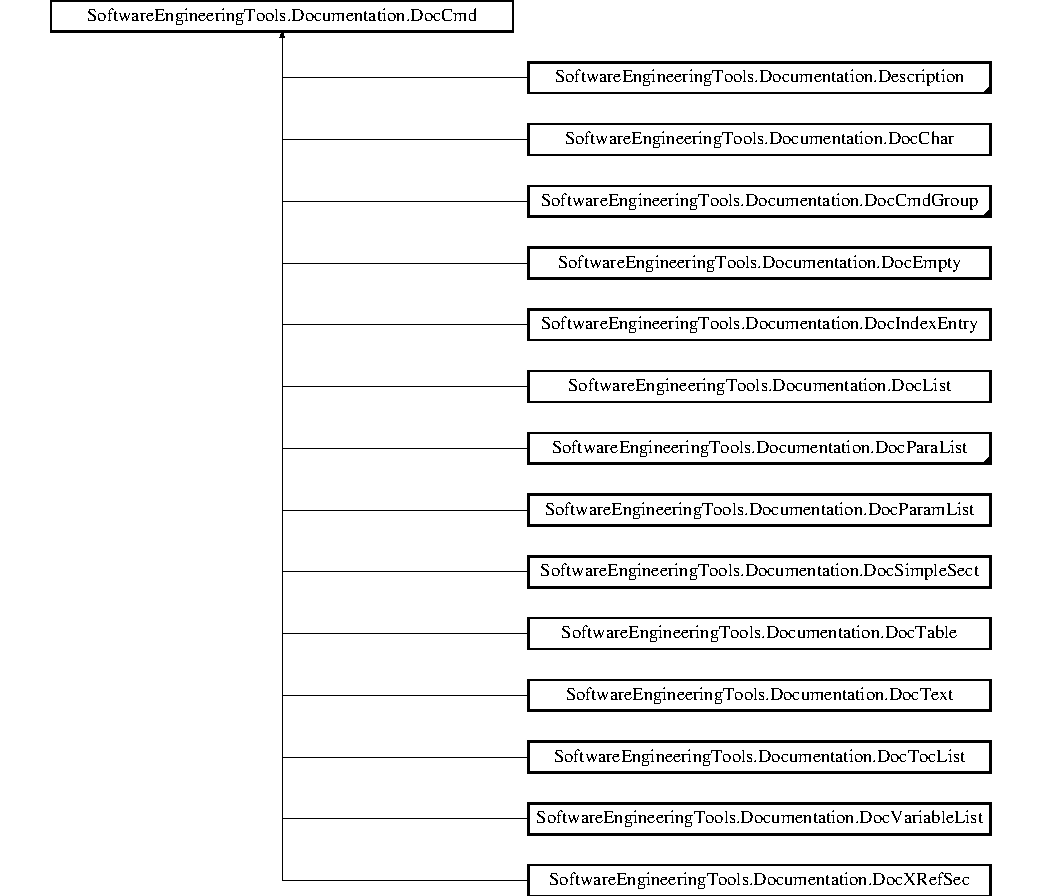
\includegraphics[height=12.000000cm]{class_software_engineering_tools_1_1_documentation_1_1_doc_cmd}
\end{center}
\end{figure}
\subsection*{Public Member Functions}
\begin{DoxyCompactItemize}
\item 
\hyperlink{class_software_engineering_tools_1_1_documentation_1_1_doc_cmd_aa5883c5254fa81621eb08bf6dcb6d676}{Doc\+Cmd} ()
\end{DoxyCompactItemize}
\subsection*{Properties}
\begin{DoxyCompactItemize}
\item 
\hyperlink{namespace_software_engineering_tools_1_1_documentation_ae0bccf4f49a76db084c1c316e5954ec9}{Doc\+Kind} \hyperlink{class_software_engineering_tools_1_1_documentation_1_1_doc_cmd_a85998cc3f4e34b4fbd9c825ffd1f72b5}{Kind}\hspace{0.3cm}{\ttfamily  \mbox{[}get, set\mbox{]}}
\end{DoxyCompactItemize}


\subsection{Detailed Description}


Definition at line 502 of file Doxygen.\+cs.



\subsection{Constructor \& Destructor Documentation}
\hypertarget{class_software_engineering_tools_1_1_documentation_1_1_doc_cmd_aa5883c5254fa81621eb08bf6dcb6d676}{\index{Software\+Engineering\+Tools\+::\+Documentation\+::\+Doc\+Cmd@{Software\+Engineering\+Tools\+::\+Documentation\+::\+Doc\+Cmd}!Doc\+Cmd@{Doc\+Cmd}}
\index{Doc\+Cmd@{Doc\+Cmd}!Software\+Engineering\+Tools\+::\+Documentation\+::\+Doc\+Cmd@{Software\+Engineering\+Tools\+::\+Documentation\+::\+Doc\+Cmd}}
\subsubsection[{Doc\+Cmd}]{\setlength{\rightskip}{0pt plus 5cm}Software\+Engineering\+Tools.\+Documentation.\+Doc\+Cmd.\+Doc\+Cmd (
\begin{DoxyParamCaption}
{}
\end{DoxyParamCaption}
)}}\label{class_software_engineering_tools_1_1_documentation_1_1_doc_cmd_aa5883c5254fa81621eb08bf6dcb6d676}


Definition at line 506 of file Doxygen.\+cs.



\subsection{Property Documentation}
\hypertarget{class_software_engineering_tools_1_1_documentation_1_1_doc_cmd_a85998cc3f4e34b4fbd9c825ffd1f72b5}{\index{Software\+Engineering\+Tools\+::\+Documentation\+::\+Doc\+Cmd@{Software\+Engineering\+Tools\+::\+Documentation\+::\+Doc\+Cmd}!Kind@{Kind}}
\index{Kind@{Kind}!Software\+Engineering\+Tools\+::\+Documentation\+::\+Doc\+Cmd@{Software\+Engineering\+Tools\+::\+Documentation\+::\+Doc\+Cmd}}
\subsubsection[{Kind}]{\setlength{\rightskip}{0pt plus 5cm}{\bf Doc\+Kind} Software\+Engineering\+Tools.\+Documentation.\+Doc\+Cmd.\+Kind\hspace{0.3cm}{\ttfamily [get]}, {\ttfamily [set]}}}\label{class_software_engineering_tools_1_1_documentation_1_1_doc_cmd_a85998cc3f4e34b4fbd9c825ffd1f72b5}


Definition at line 504 of file Doxygen.\+cs.



The documentation for this class was generated from the following file\+:\begin{DoxyCompactItemize}
\item 
Api\+Doc\+Lib/\hyperlink{_doxygen_8cs}{Doxygen.\+cs}\end{DoxyCompactItemize}

\hypertarget{class_software_engineering_tools_1_1_documentation_1_1_doc_cmd_group}{\section{Software\+Engineering\+Tools.\+Documentation.\+Doc\+Cmd\+Group Class Reference}
\label{class_software_engineering_tools_1_1_documentation_1_1_doc_cmd_group}\index{Software\+Engineering\+Tools.\+Documentation.\+Doc\+Cmd\+Group@{Software\+Engineering\+Tools.\+Documentation.\+Doc\+Cmd\+Group}}
}
Inheritance diagram for Software\+Engineering\+Tools.\+Documentation.\+Doc\+Cmd\+Group\+:\begin{figure}[H]
\begin{center}
\leavevmode
\includegraphics[height=11.461988cm]{class_software_engineering_tools_1_1_documentation_1_1_doc_cmd_group}
\end{center}
\end{figure}
\subsection*{Public Member Functions}
\begin{DoxyCompactItemize}
\item 
\hyperlink{class_software_engineering_tools_1_1_documentation_1_1_doc_cmd_group_adc2876c88d61e89b18cf833132a0def5}{Doc\+Cmd\+Group} ()
\end{DoxyCompactItemize}
\subsection*{Properties}
\begin{DoxyCompactItemize}
\item 
\hyperlink{namespace_software_engineering_tools_1_1_documentation_ae0bccf4f49a76db084c1c316e5954ec9a4ee29ca12c7d126654bd0e5275de6135}{List}$<$ \hyperlink{class_software_engineering_tools_1_1_documentation_1_1_doc_cmd}{Doc\+Cmd} $>$ \hyperlink{class_software_engineering_tools_1_1_documentation_1_1_doc_cmd_group_ac6f2fb2ec29fc2eeac0f46740b2c5144}{Commands}\hspace{0.3cm}{\ttfamily  \mbox{[}get, set\mbox{]}}
\end{DoxyCompactItemize}


\subsection{Detailed Description}


Definition at line 512 of file Doxygen.\+cs.



\subsection{Constructor \& Destructor Documentation}
\hypertarget{class_software_engineering_tools_1_1_documentation_1_1_doc_cmd_group_adc2876c88d61e89b18cf833132a0def5}{\index{Software\+Engineering\+Tools\+::\+Documentation\+::\+Doc\+Cmd\+Group@{Software\+Engineering\+Tools\+::\+Documentation\+::\+Doc\+Cmd\+Group}!Doc\+Cmd\+Group@{Doc\+Cmd\+Group}}
\index{Doc\+Cmd\+Group@{Doc\+Cmd\+Group}!Software\+Engineering\+Tools\+::\+Documentation\+::\+Doc\+Cmd\+Group@{Software\+Engineering\+Tools\+::\+Documentation\+::\+Doc\+Cmd\+Group}}
\subsubsection[{Doc\+Cmd\+Group}]{\setlength{\rightskip}{0pt plus 5cm}Software\+Engineering\+Tools.\+Documentation.\+Doc\+Cmd\+Group.\+Doc\+Cmd\+Group (
\begin{DoxyParamCaption}
{}
\end{DoxyParamCaption}
)}}\label{class_software_engineering_tools_1_1_documentation_1_1_doc_cmd_group_adc2876c88d61e89b18cf833132a0def5}


Definition at line 516 of file Doxygen.\+cs.



\subsection{Property Documentation}
\hypertarget{class_software_engineering_tools_1_1_documentation_1_1_doc_cmd_group_ac6f2fb2ec29fc2eeac0f46740b2c5144}{\index{Software\+Engineering\+Tools\+::\+Documentation\+::\+Doc\+Cmd\+Group@{Software\+Engineering\+Tools\+::\+Documentation\+::\+Doc\+Cmd\+Group}!Commands@{Commands}}
\index{Commands@{Commands}!Software\+Engineering\+Tools\+::\+Documentation\+::\+Doc\+Cmd\+Group@{Software\+Engineering\+Tools\+::\+Documentation\+::\+Doc\+Cmd\+Group}}
\subsubsection[{Commands}]{\setlength{\rightskip}{0pt plus 5cm}{\bf List}$<${\bf Doc\+Cmd}$>$ Software\+Engineering\+Tools.\+Documentation.\+Doc\+Cmd\+Group.\+Commands\hspace{0.3cm}{\ttfamily [get]}, {\ttfamily [set]}}}\label{class_software_engineering_tools_1_1_documentation_1_1_doc_cmd_group_ac6f2fb2ec29fc2eeac0f46740b2c5144}


Definition at line 514 of file Doxygen.\+cs.



The documentation for this class was generated from the following file\+:\begin{DoxyCompactItemize}
\item 
Api\+Doc\+Lib/\hyperlink{_doxygen_8cs}{Doxygen.\+cs}\end{DoxyCompactItemize}

\hypertarget{class_software_engineering_tools_1_1_documentation_1_1_doc_copy}{\section{Software\+Engineering\+Tools.\+Documentation.\+Doc\+Copy Class Reference}
\label{class_software_engineering_tools_1_1_documentation_1_1_doc_copy}\index{Software\+Engineering\+Tools.\+Documentation.\+Doc\+Copy@{Software\+Engineering\+Tools.\+Documentation.\+Doc\+Copy}}
}
Inheritance diagram for Software\+Engineering\+Tools.\+Documentation.\+Doc\+Copy\+:\begin{figure}[H]
\begin{center}
\leavevmode
\includegraphics[height=4.000000cm]{class_software_engineering_tools_1_1_documentation_1_1_doc_copy}
\end{center}
\end{figure}
\subsection*{Public Member Functions}
\begin{DoxyCompactItemize}
\item 
\hyperlink{class_software_engineering_tools_1_1_documentation_1_1_doc_copy_a28ae090505592eb981df107a0e76e1c5}{Doc\+Copy} ()
\end{DoxyCompactItemize}
\subsection*{Additional Inherited Members}


\subsection{Detailed Description}


Definition at line 1030 of file Doxygen.\+cs.



\subsection{Constructor \& Destructor Documentation}
\hypertarget{class_software_engineering_tools_1_1_documentation_1_1_doc_copy_a28ae090505592eb981df107a0e76e1c5}{\index{Software\+Engineering\+Tools\+::\+Documentation\+::\+Doc\+Copy@{Software\+Engineering\+Tools\+::\+Documentation\+::\+Doc\+Copy}!Doc\+Copy@{Doc\+Copy}}
\index{Doc\+Copy@{Doc\+Copy}!Software\+Engineering\+Tools\+::\+Documentation\+::\+Doc\+Copy@{Software\+Engineering\+Tools\+::\+Documentation\+::\+Doc\+Copy}}
\subsubsection[{Doc\+Copy}]{\setlength{\rightskip}{0pt plus 5cm}Software\+Engineering\+Tools.\+Documentation.\+Doc\+Copy.\+Doc\+Copy (
\begin{DoxyParamCaption}
{}
\end{DoxyParamCaption}
)}}\label{class_software_engineering_tools_1_1_documentation_1_1_doc_copy_a28ae090505592eb981df107a0e76e1c5}


Definition at line 1032 of file Doxygen.\+cs.



The documentation for this class was generated from the following file\+:\begin{DoxyCompactItemize}
\item 
Api\+Doc\+Lib/\hyperlink{_doxygen_8cs}{Doxygen.\+cs}\end{DoxyCompactItemize}

\hypertarget{class_software_engineering_tools_1_1_documentation_1_1_doc_dot_file}{\section{Software\+Engineering\+Tools.\+Documentation.\+Doc\+Dot\+File Class Reference}
\label{class_software_engineering_tools_1_1_documentation_1_1_doc_dot_file}\index{Software\+Engineering\+Tools.\+Documentation.\+Doc\+Dot\+File@{Software\+Engineering\+Tools.\+Documentation.\+Doc\+Dot\+File}}
}
Inheritance diagram for Software\+Engineering\+Tools.\+Documentation.\+Doc\+Dot\+File\+:\begin{figure}[H]
\begin{center}
\leavevmode
\includegraphics[height=3.000000cm]{class_software_engineering_tools_1_1_documentation_1_1_doc_dot_file}
\end{center}
\end{figure}
\subsection*{Public Member Functions}
\begin{DoxyCompactItemize}
\item 
\hyperlink{class_software_engineering_tools_1_1_documentation_1_1_doc_dot_file_ae447910a47c25d6a8bdce0b849367fe9}{Doc\+Dot\+File} ()
\end{DoxyCompactItemize}
\subsection*{Properties}
\begin{DoxyCompactItemize}
\item 
string \hyperlink{class_software_engineering_tools_1_1_documentation_1_1_doc_dot_file_ac362448a9bea0682d1f2aa7887e75e11}{Id}\hspace{0.3cm}{\ttfamily  \mbox{[}get, set\mbox{]}}
\end{DoxyCompactItemize}


\subsection{Detailed Description}


Definition at line 920 of file Doxygen.\+cs.



\subsection{Constructor \& Destructor Documentation}
\hypertarget{class_software_engineering_tools_1_1_documentation_1_1_doc_dot_file_ae447910a47c25d6a8bdce0b849367fe9}{\index{Software\+Engineering\+Tools\+::\+Documentation\+::\+Doc\+Dot\+File@{Software\+Engineering\+Tools\+::\+Documentation\+::\+Doc\+Dot\+File}!Doc\+Dot\+File@{Doc\+Dot\+File}}
\index{Doc\+Dot\+File@{Doc\+Dot\+File}!Software\+Engineering\+Tools\+::\+Documentation\+::\+Doc\+Dot\+File@{Software\+Engineering\+Tools\+::\+Documentation\+::\+Doc\+Dot\+File}}
\subsubsection[{Doc\+Dot\+File}]{\setlength{\rightskip}{0pt plus 5cm}Software\+Engineering\+Tools.\+Documentation.\+Doc\+Dot\+File.\+Doc\+Dot\+File (
\begin{DoxyParamCaption}
{}
\end{DoxyParamCaption}
)}}\label{class_software_engineering_tools_1_1_documentation_1_1_doc_dot_file_ae447910a47c25d6a8bdce0b849367fe9}


Definition at line 924 of file Doxygen.\+cs.



\subsection{Property Documentation}
\hypertarget{class_software_engineering_tools_1_1_documentation_1_1_doc_dot_file_ac362448a9bea0682d1f2aa7887e75e11}{\index{Software\+Engineering\+Tools\+::\+Documentation\+::\+Doc\+Dot\+File@{Software\+Engineering\+Tools\+::\+Documentation\+::\+Doc\+Dot\+File}!Id@{Id}}
\index{Id@{Id}!Software\+Engineering\+Tools\+::\+Documentation\+::\+Doc\+Dot\+File@{Software\+Engineering\+Tools\+::\+Documentation\+::\+Doc\+Dot\+File}}
\subsubsection[{Id}]{\setlength{\rightskip}{0pt plus 5cm}string Software\+Engineering\+Tools.\+Documentation.\+Doc\+Dot\+File.\+Id\hspace{0.3cm}{\ttfamily [get]}, {\ttfamily [set]}}}\label{class_software_engineering_tools_1_1_documentation_1_1_doc_dot_file_ac362448a9bea0682d1f2aa7887e75e11}


Definition at line 922 of file Doxygen.\+cs.



The documentation for this class was generated from the following file\+:\begin{DoxyCompactItemize}
\item 
Api\+Doc\+Lib/\hyperlink{_doxygen_8cs}{Doxygen.\+cs}\end{DoxyCompactItemize}

\hypertarget{class_software_engineering_tools_1_1_documentation_1_1_doc_empty}{\section{Software\+Engineering\+Tools.\+Documentation.\+Doc\+Empty Class Reference}
\label{class_software_engineering_tools_1_1_documentation_1_1_doc_empty}\index{Software\+Engineering\+Tools.\+Documentation.\+Doc\+Empty@{Software\+Engineering\+Tools.\+Documentation.\+Doc\+Empty}}
}
Inheritance diagram for Software\+Engineering\+Tools.\+Documentation.\+Doc\+Empty\+:\begin{figure}[H]
\begin{center}
\leavevmode
\includegraphics[height=2.000000cm]{class_software_engineering_tools_1_1_documentation_1_1_doc_empty}
\end{center}
\end{figure}
\subsection*{Public Member Functions}
\begin{DoxyCompactItemize}
\item 
\hyperlink{class_software_engineering_tools_1_1_documentation_1_1_doc_empty_adc90b20452309d000ebe98d8b1b1eda5}{Doc\+Empty} ()
\end{DoxyCompactItemize}
\subsection*{Properties}
\begin{DoxyCompactItemize}
\item 
\hyperlink{namespace_software_engineering_tools_1_1_documentation_a4a8017aa254d1d05b03db5132b7dd3a7}{Doc\+Empty\+Kind} \hyperlink{class_software_engineering_tools_1_1_documentation_1_1_doc_empty_a193949a8c51dd660fb77a8b6f419f9ea}{Empty\+Kind}\hspace{0.3cm}{\ttfamily  \mbox{[}get, set\mbox{]}}
\end{DoxyCompactItemize}


\subsection{Detailed Description}


Definition at line 573 of file Doxygen.\+cs.



\subsection{Constructor \& Destructor Documentation}
\hypertarget{class_software_engineering_tools_1_1_documentation_1_1_doc_empty_adc90b20452309d000ebe98d8b1b1eda5}{\index{Software\+Engineering\+Tools\+::\+Documentation\+::\+Doc\+Empty@{Software\+Engineering\+Tools\+::\+Documentation\+::\+Doc\+Empty}!Doc\+Empty@{Doc\+Empty}}
\index{Doc\+Empty@{Doc\+Empty}!Software\+Engineering\+Tools\+::\+Documentation\+::\+Doc\+Empty@{Software\+Engineering\+Tools\+::\+Documentation\+::\+Doc\+Empty}}
\subsubsection[{Doc\+Empty}]{\setlength{\rightskip}{0pt plus 5cm}Software\+Engineering\+Tools.\+Documentation.\+Doc\+Empty.\+Doc\+Empty (
\begin{DoxyParamCaption}
{}
\end{DoxyParamCaption}
)}}\label{class_software_engineering_tools_1_1_documentation_1_1_doc_empty_adc90b20452309d000ebe98d8b1b1eda5}


Definition at line 577 of file Doxygen.\+cs.



\subsection{Property Documentation}
\hypertarget{class_software_engineering_tools_1_1_documentation_1_1_doc_empty_a193949a8c51dd660fb77a8b6f419f9ea}{\index{Software\+Engineering\+Tools\+::\+Documentation\+::\+Doc\+Empty@{Software\+Engineering\+Tools\+::\+Documentation\+::\+Doc\+Empty}!Empty\+Kind@{Empty\+Kind}}
\index{Empty\+Kind@{Empty\+Kind}!Software\+Engineering\+Tools\+::\+Documentation\+::\+Doc\+Empty@{Software\+Engineering\+Tools\+::\+Documentation\+::\+Doc\+Empty}}
\subsubsection[{Empty\+Kind}]{\setlength{\rightskip}{0pt plus 5cm}{\bf Doc\+Empty\+Kind} Software\+Engineering\+Tools.\+Documentation.\+Doc\+Empty.\+Empty\+Kind\hspace{0.3cm}{\ttfamily [get]}, {\ttfamily [set]}}}\label{class_software_engineering_tools_1_1_documentation_1_1_doc_empty_a193949a8c51dd660fb77a8b6f419f9ea}


Definition at line 575 of file Doxygen.\+cs.



The documentation for this class was generated from the following file\+:\begin{DoxyCompactItemize}
\item 
Api\+Doc\+Lib/\hyperlink{_doxygen_8cs}{Doxygen.\+cs}\end{DoxyCompactItemize}

\hypertarget{class_software_engineering_tools_1_1_documentation_1_1_doc_formula}{\section{Software\+Engineering\+Tools.\+Documentation.\+Doc\+Formula Class Reference}
\label{class_software_engineering_tools_1_1_documentation_1_1_doc_formula}\index{Software\+Engineering\+Tools.\+Documentation.\+Doc\+Formula@{Software\+Engineering\+Tools.\+Documentation.\+Doc\+Formula}}
}
Inheritance diagram for Software\+Engineering\+Tools.\+Documentation.\+Doc\+Formula\+:\begin{figure}[H]
\begin{center}
\leavevmode
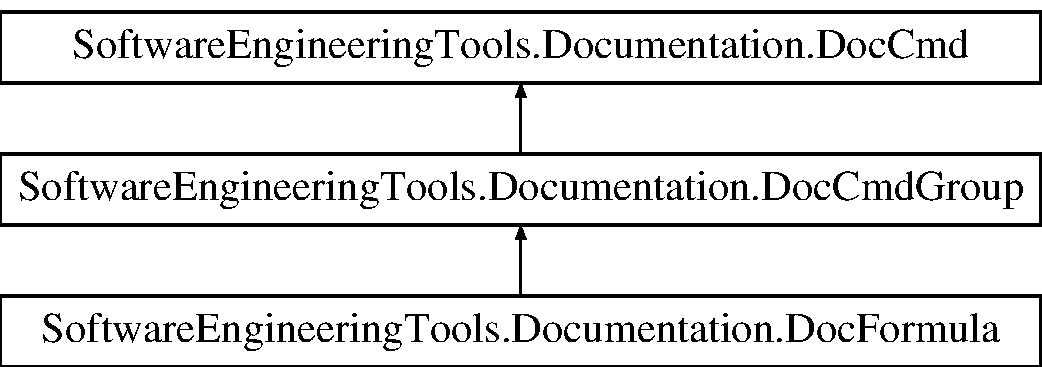
\includegraphics[height=3.000000cm]{class_software_engineering_tools_1_1_documentation_1_1_doc_formula}
\end{center}
\end{figure}
\subsection*{Public Member Functions}
\begin{DoxyCompactItemize}
\item 
\hyperlink{class_software_engineering_tools_1_1_documentation_1_1_doc_formula_a12e0223aeac7a696926fa4c0dbbadacd}{Doc\+Formula} ()
\end{DoxyCompactItemize}
\subsection*{Properties}
\begin{DoxyCompactItemize}
\item 
string \hyperlink{class_software_engineering_tools_1_1_documentation_1_1_doc_formula_af0946e5bef66d6f9ad930939c5ddcc51}{Id}\hspace{0.3cm}{\ttfamily  \mbox{[}get, set\mbox{]}}
\end{DoxyCompactItemize}


\subsection{Detailed Description}


Definition at line 726 of file Doxygen.\+cs.



\subsection{Constructor \& Destructor Documentation}
\hypertarget{class_software_engineering_tools_1_1_documentation_1_1_doc_formula_a12e0223aeac7a696926fa4c0dbbadacd}{\index{Software\+Engineering\+Tools\+::\+Documentation\+::\+Doc\+Formula@{Software\+Engineering\+Tools\+::\+Documentation\+::\+Doc\+Formula}!Doc\+Formula@{Doc\+Formula}}
\index{Doc\+Formula@{Doc\+Formula}!Software\+Engineering\+Tools\+::\+Documentation\+::\+Doc\+Formula@{Software\+Engineering\+Tools\+::\+Documentation\+::\+Doc\+Formula}}
\subsubsection[{Doc\+Formula}]{\setlength{\rightskip}{0pt plus 5cm}Software\+Engineering\+Tools.\+Documentation.\+Doc\+Formula.\+Doc\+Formula (
\begin{DoxyParamCaption}
{}
\end{DoxyParamCaption}
)}}\label{class_software_engineering_tools_1_1_documentation_1_1_doc_formula_a12e0223aeac7a696926fa4c0dbbadacd}


Definition at line 730 of file Doxygen.\+cs.



\subsection{Property Documentation}
\hypertarget{class_software_engineering_tools_1_1_documentation_1_1_doc_formula_af0946e5bef66d6f9ad930939c5ddcc51}{\index{Software\+Engineering\+Tools\+::\+Documentation\+::\+Doc\+Formula@{Software\+Engineering\+Tools\+::\+Documentation\+::\+Doc\+Formula}!Id@{Id}}
\index{Id@{Id}!Software\+Engineering\+Tools\+::\+Documentation\+::\+Doc\+Formula@{Software\+Engineering\+Tools\+::\+Documentation\+::\+Doc\+Formula}}
\subsubsection[{Id}]{\setlength{\rightskip}{0pt plus 5cm}string Software\+Engineering\+Tools.\+Documentation.\+Doc\+Formula.\+Id\hspace{0.3cm}{\ttfamily [get]}, {\ttfamily [set]}}}\label{class_software_engineering_tools_1_1_documentation_1_1_doc_formula_af0946e5bef66d6f9ad930939c5ddcc51}


Definition at line 728 of file Doxygen.\+cs.



The documentation for this class was generated from the following file\+:\begin{DoxyCompactItemize}
\item 
Api\+Doc\+Lib/\hyperlink{_doxygen_8cs}{Doxygen.\+cs}\end{DoxyCompactItemize}

\hypertarget{class_software_engineering_tools_1_1_documentation_1_1_doc_heading}{\section{Software\+Engineering\+Tools.\+Documentation.\+Doc\+Heading Class Reference}
\label{class_software_engineering_tools_1_1_documentation_1_1_doc_heading}\index{Software\+Engineering\+Tools.\+Documentation.\+Doc\+Heading@{Software\+Engineering\+Tools.\+Documentation.\+Doc\+Heading}}
}
Inheritance diagram for Software\+Engineering\+Tools.\+Documentation.\+Doc\+Heading\+:\begin{figure}[H]
\begin{center}
\leavevmode
\includegraphics[height=3.000000cm]{class_software_engineering_tools_1_1_documentation_1_1_doc_heading}
\end{center}
\end{figure}
\subsection*{Public Member Functions}
\begin{DoxyCompactItemize}
\item 
\hyperlink{class_software_engineering_tools_1_1_documentation_1_1_doc_heading_a99e5ae13865091d9d2db930066de75c6}{Doc\+Heading} ()
\end{DoxyCompactItemize}
\subsection*{Properties}
\begin{DoxyCompactItemize}
\item 
\hyperlink{namespace_software_engineering_tools_1_1_documentation_a4a8017aa254d1d05b03db5132b7dd3a7afa7153f7ed1cb6c0fcf2ffb2fac21748}{int} \hyperlink{class_software_engineering_tools_1_1_documentation_1_1_doc_heading_ab4db448b267cbef63884b9e6686e7e65}{Level}\hspace{0.3cm}{\ttfamily  \mbox{[}get, set\mbox{]}}
\end{DoxyCompactItemize}


\subsection{Detailed Description}


Definition at line 844 of file Doxygen.\+cs.



\subsection{Constructor \& Destructor Documentation}
\hypertarget{class_software_engineering_tools_1_1_documentation_1_1_doc_heading_a99e5ae13865091d9d2db930066de75c6}{\index{Software\+Engineering\+Tools\+::\+Documentation\+::\+Doc\+Heading@{Software\+Engineering\+Tools\+::\+Documentation\+::\+Doc\+Heading}!Doc\+Heading@{Doc\+Heading}}
\index{Doc\+Heading@{Doc\+Heading}!Software\+Engineering\+Tools\+::\+Documentation\+::\+Doc\+Heading@{Software\+Engineering\+Tools\+::\+Documentation\+::\+Doc\+Heading}}
\subsubsection[{Doc\+Heading}]{\setlength{\rightskip}{0pt plus 5cm}Software\+Engineering\+Tools.\+Documentation.\+Doc\+Heading.\+Doc\+Heading (
\begin{DoxyParamCaption}
{}
\end{DoxyParamCaption}
)}}\label{class_software_engineering_tools_1_1_documentation_1_1_doc_heading_a99e5ae13865091d9d2db930066de75c6}


Definition at line 848 of file Doxygen.\+cs.



\subsection{Property Documentation}
\hypertarget{class_software_engineering_tools_1_1_documentation_1_1_doc_heading_ab4db448b267cbef63884b9e6686e7e65}{\index{Software\+Engineering\+Tools\+::\+Documentation\+::\+Doc\+Heading@{Software\+Engineering\+Tools\+::\+Documentation\+::\+Doc\+Heading}!Level@{Level}}
\index{Level@{Level}!Software\+Engineering\+Tools\+::\+Documentation\+::\+Doc\+Heading@{Software\+Engineering\+Tools\+::\+Documentation\+::\+Doc\+Heading}}
\subsubsection[{Level}]{\setlength{\rightskip}{0pt plus 5cm}{\bf int} Software\+Engineering\+Tools.\+Documentation.\+Doc\+Heading.\+Level\hspace{0.3cm}{\ttfamily [get]}, {\ttfamily [set]}}}\label{class_software_engineering_tools_1_1_documentation_1_1_doc_heading_ab4db448b267cbef63884b9e6686e7e65}


Definition at line 846 of file Doxygen.\+cs.



The documentation for this class was generated from the following file\+:\begin{DoxyCompactItemize}
\item 
Api\+Doc\+Lib/\hyperlink{_doxygen_8cs}{Doxygen.\+cs}\end{DoxyCompactItemize}

\hypertarget{class_software_engineering_tools_1_1_documentation_1_1_doc_image}{\section{Software\+Engineering\+Tools.\+Documentation.\+Doc\+Image Class Reference}
\label{class_software_engineering_tools_1_1_documentation_1_1_doc_image}\index{Software\+Engineering\+Tools.\+Documentation.\+Doc\+Image@{Software\+Engineering\+Tools.\+Documentation.\+Doc\+Image}}
}
Inheritance diagram for Software\+Engineering\+Tools.\+Documentation.\+Doc\+Image\+:\begin{figure}[H]
\begin{center}
\leavevmode
\includegraphics[height=3.000000cm]{class_software_engineering_tools_1_1_documentation_1_1_doc_image}
\end{center}
\end{figure}
\subsection*{Public Member Functions}
\begin{DoxyCompactItemize}
\item 
\hyperlink{class_software_engineering_tools_1_1_documentation_1_1_doc_image_abffb80615eb570220bd038dd88c93ffe}{Doc\+Image} ()
\end{DoxyCompactItemize}
\subsection*{Properties}
\begin{DoxyCompactItemize}
\item 
\hyperlink{namespace_software_engineering_tools_1_1_documentation_ab21398cff938858e1d9ebdc672403015}{Doc\+Image\+Kind} \hyperlink{class_software_engineering_tools_1_1_documentation_1_1_doc_image_aa73b29c8c230474bd80d01dfa25555ff}{Image\+Kind}\hspace{0.3cm}{\ttfamily  \mbox{[}get, set\mbox{]}}
\item 
string \hyperlink{class_software_engineering_tools_1_1_documentation_1_1_doc_image_a18a4f96074d4dad07c0811896dd4305b}{Name}\hspace{0.3cm}{\ttfamily  \mbox{[}get, set\mbox{]}}
\item 
string \hyperlink{class_software_engineering_tools_1_1_documentation_1_1_doc_image_a697f5c432b0a513b53dec61f66ad43ee}{Width}\hspace{0.3cm}{\ttfamily  \mbox{[}get, set\mbox{]}}
\item 
string \hyperlink{class_software_engineering_tools_1_1_documentation_1_1_doc_image_a13b59f2f69ce4f465c966637480cef6c}{Height}\hspace{0.3cm}{\ttfamily  \mbox{[}get, set\mbox{]}}
\end{DoxyCompactItemize}


\subsection{Detailed Description}


Definition at line 900 of file Doxygen.\+cs.



\subsection{Constructor \& Destructor Documentation}
\hypertarget{class_software_engineering_tools_1_1_documentation_1_1_doc_image_abffb80615eb570220bd038dd88c93ffe}{\index{Software\+Engineering\+Tools\+::\+Documentation\+::\+Doc\+Image@{Software\+Engineering\+Tools\+::\+Documentation\+::\+Doc\+Image}!Doc\+Image@{Doc\+Image}}
\index{Doc\+Image@{Doc\+Image}!Software\+Engineering\+Tools\+::\+Documentation\+::\+Doc\+Image@{Software\+Engineering\+Tools\+::\+Documentation\+::\+Doc\+Image}}
\subsubsection[{Doc\+Image}]{\setlength{\rightskip}{0pt plus 5cm}Software\+Engineering\+Tools.\+Documentation.\+Doc\+Image.\+Doc\+Image (
\begin{DoxyParamCaption}
{}
\end{DoxyParamCaption}
)}}\label{class_software_engineering_tools_1_1_documentation_1_1_doc_image_abffb80615eb570220bd038dd88c93ffe}


Definition at line 907 of file Doxygen.\+cs.



\subsection{Property Documentation}
\hypertarget{class_software_engineering_tools_1_1_documentation_1_1_doc_image_a13b59f2f69ce4f465c966637480cef6c}{\index{Software\+Engineering\+Tools\+::\+Documentation\+::\+Doc\+Image@{Software\+Engineering\+Tools\+::\+Documentation\+::\+Doc\+Image}!Height@{Height}}
\index{Height@{Height}!Software\+Engineering\+Tools\+::\+Documentation\+::\+Doc\+Image@{Software\+Engineering\+Tools\+::\+Documentation\+::\+Doc\+Image}}
\subsubsection[{Height}]{\setlength{\rightskip}{0pt plus 5cm}string Software\+Engineering\+Tools.\+Documentation.\+Doc\+Image.\+Height\hspace{0.3cm}{\ttfamily [get]}, {\ttfamily [set]}}}\label{class_software_engineering_tools_1_1_documentation_1_1_doc_image_a13b59f2f69ce4f465c966637480cef6c}


Definition at line 905 of file Doxygen.\+cs.

\hypertarget{class_software_engineering_tools_1_1_documentation_1_1_doc_image_aa73b29c8c230474bd80d01dfa25555ff}{\index{Software\+Engineering\+Tools\+::\+Documentation\+::\+Doc\+Image@{Software\+Engineering\+Tools\+::\+Documentation\+::\+Doc\+Image}!Image\+Kind@{Image\+Kind}}
\index{Image\+Kind@{Image\+Kind}!Software\+Engineering\+Tools\+::\+Documentation\+::\+Doc\+Image@{Software\+Engineering\+Tools\+::\+Documentation\+::\+Doc\+Image}}
\subsubsection[{Image\+Kind}]{\setlength{\rightskip}{0pt plus 5cm}{\bf Doc\+Image\+Kind} Software\+Engineering\+Tools.\+Documentation.\+Doc\+Image.\+Image\+Kind\hspace{0.3cm}{\ttfamily [get]}, {\ttfamily [set]}}}\label{class_software_engineering_tools_1_1_documentation_1_1_doc_image_aa73b29c8c230474bd80d01dfa25555ff}


Definition at line 902 of file Doxygen.\+cs.

\hypertarget{class_software_engineering_tools_1_1_documentation_1_1_doc_image_a18a4f96074d4dad07c0811896dd4305b}{\index{Software\+Engineering\+Tools\+::\+Documentation\+::\+Doc\+Image@{Software\+Engineering\+Tools\+::\+Documentation\+::\+Doc\+Image}!Name@{Name}}
\index{Name@{Name}!Software\+Engineering\+Tools\+::\+Documentation\+::\+Doc\+Image@{Software\+Engineering\+Tools\+::\+Documentation\+::\+Doc\+Image}}
\subsubsection[{Name}]{\setlength{\rightskip}{0pt plus 5cm}string Software\+Engineering\+Tools.\+Documentation.\+Doc\+Image.\+Name\hspace{0.3cm}{\ttfamily [get]}, {\ttfamily [set]}}}\label{class_software_engineering_tools_1_1_documentation_1_1_doc_image_a18a4f96074d4dad07c0811896dd4305b}


Definition at line 903 of file Doxygen.\+cs.

\hypertarget{class_software_engineering_tools_1_1_documentation_1_1_doc_image_a697f5c432b0a513b53dec61f66ad43ee}{\index{Software\+Engineering\+Tools\+::\+Documentation\+::\+Doc\+Image@{Software\+Engineering\+Tools\+::\+Documentation\+::\+Doc\+Image}!Width@{Width}}
\index{Width@{Width}!Software\+Engineering\+Tools\+::\+Documentation\+::\+Doc\+Image@{Software\+Engineering\+Tools\+::\+Documentation\+::\+Doc\+Image}}
\subsubsection[{Width}]{\setlength{\rightskip}{0pt plus 5cm}string Software\+Engineering\+Tools.\+Documentation.\+Doc\+Image.\+Width\hspace{0.3cm}{\ttfamily [get]}, {\ttfamily [set]}}}\label{class_software_engineering_tools_1_1_documentation_1_1_doc_image_a697f5c432b0a513b53dec61f66ad43ee}


Definition at line 904 of file Doxygen.\+cs.



The documentation for this class was generated from the following file\+:\begin{DoxyCompactItemize}
\item 
Api\+Doc\+Lib/\hyperlink{_doxygen_8cs}{Doxygen.\+cs}\end{DoxyCompactItemize}

\hypertarget{class_software_engineering_tools_1_1_documentation_1_1_doc_index_entry}{\section{Software\+Engineering\+Tools.\+Documentation.\+Doc\+Index\+Entry Class Reference}
\label{class_software_engineering_tools_1_1_documentation_1_1_doc_index_entry}\index{Software\+Engineering\+Tools.\+Documentation.\+Doc\+Index\+Entry@{Software\+Engineering\+Tools.\+Documentation.\+Doc\+Index\+Entry}}
}
Inheritance diagram for Software\+Engineering\+Tools.\+Documentation.\+Doc\+Index\+Entry\+:\begin{figure}[H]
\begin{center}
\leavevmode
\includegraphics[height=2.000000cm]{class_software_engineering_tools_1_1_documentation_1_1_doc_index_entry}
\end{center}
\end{figure}
\subsection*{Public Member Functions}
\begin{DoxyCompactItemize}
\item 
\hyperlink{class_software_engineering_tools_1_1_documentation_1_1_doc_index_entry_af4d7a6e93f1384f3e1aec974f294986d}{Doc\+Index\+Entry} ()
\end{DoxyCompactItemize}
\subsection*{Properties}
\begin{DoxyCompactItemize}
\item 
string \hyperlink{class_software_engineering_tools_1_1_documentation_1_1_doc_index_entry_aec1df763bc86dffdc381693aefe66131}{Primary\+Entry}\hspace{0.3cm}{\ttfamily  \mbox{[}get, set\mbox{]}}
\item 
string \hyperlink{class_software_engineering_tools_1_1_documentation_1_1_doc_index_entry_a0c508fb0b715f0eb8709ed6ba728f0ce}{Secondary\+Entry}\hspace{0.3cm}{\ttfamily  \mbox{[}get, set\mbox{]}}
\end{DoxyCompactItemize}


\subsection{Detailed Description}


Definition at line 755 of file Doxygen.\+cs.



\subsection{Constructor \& Destructor Documentation}
\hypertarget{class_software_engineering_tools_1_1_documentation_1_1_doc_index_entry_af4d7a6e93f1384f3e1aec974f294986d}{\index{Software\+Engineering\+Tools\+::\+Documentation\+::\+Doc\+Index\+Entry@{Software\+Engineering\+Tools\+::\+Documentation\+::\+Doc\+Index\+Entry}!Doc\+Index\+Entry@{Doc\+Index\+Entry}}
\index{Doc\+Index\+Entry@{Doc\+Index\+Entry}!Software\+Engineering\+Tools\+::\+Documentation\+::\+Doc\+Index\+Entry@{Software\+Engineering\+Tools\+::\+Documentation\+::\+Doc\+Index\+Entry}}
\subsubsection[{Doc\+Index\+Entry}]{\setlength{\rightskip}{0pt plus 5cm}Software\+Engineering\+Tools.\+Documentation.\+Doc\+Index\+Entry.\+Doc\+Index\+Entry (
\begin{DoxyParamCaption}
{}
\end{DoxyParamCaption}
)}}\label{class_software_engineering_tools_1_1_documentation_1_1_doc_index_entry_af4d7a6e93f1384f3e1aec974f294986d}


Definition at line 760 of file Doxygen.\+cs.



\subsection{Property Documentation}
\hypertarget{class_software_engineering_tools_1_1_documentation_1_1_doc_index_entry_aec1df763bc86dffdc381693aefe66131}{\index{Software\+Engineering\+Tools\+::\+Documentation\+::\+Doc\+Index\+Entry@{Software\+Engineering\+Tools\+::\+Documentation\+::\+Doc\+Index\+Entry}!Primary\+Entry@{Primary\+Entry}}
\index{Primary\+Entry@{Primary\+Entry}!Software\+Engineering\+Tools\+::\+Documentation\+::\+Doc\+Index\+Entry@{Software\+Engineering\+Tools\+::\+Documentation\+::\+Doc\+Index\+Entry}}
\subsubsection[{Primary\+Entry}]{\setlength{\rightskip}{0pt plus 5cm}string Software\+Engineering\+Tools.\+Documentation.\+Doc\+Index\+Entry.\+Primary\+Entry\hspace{0.3cm}{\ttfamily [get]}, {\ttfamily [set]}}}\label{class_software_engineering_tools_1_1_documentation_1_1_doc_index_entry_aec1df763bc86dffdc381693aefe66131}


Definition at line 757 of file Doxygen.\+cs.

\hypertarget{class_software_engineering_tools_1_1_documentation_1_1_doc_index_entry_a0c508fb0b715f0eb8709ed6ba728f0ce}{\index{Software\+Engineering\+Tools\+::\+Documentation\+::\+Doc\+Index\+Entry@{Software\+Engineering\+Tools\+::\+Documentation\+::\+Doc\+Index\+Entry}!Secondary\+Entry@{Secondary\+Entry}}
\index{Secondary\+Entry@{Secondary\+Entry}!Software\+Engineering\+Tools\+::\+Documentation\+::\+Doc\+Index\+Entry@{Software\+Engineering\+Tools\+::\+Documentation\+::\+Doc\+Index\+Entry}}
\subsubsection[{Secondary\+Entry}]{\setlength{\rightskip}{0pt plus 5cm}string Software\+Engineering\+Tools.\+Documentation.\+Doc\+Index\+Entry.\+Secondary\+Entry\hspace{0.3cm}{\ttfamily [get]}, {\ttfamily [set]}}}\label{class_software_engineering_tools_1_1_documentation_1_1_doc_index_entry_a0c508fb0b715f0eb8709ed6ba728f0ce}


Definition at line 758 of file Doxygen.\+cs.



The documentation for this class was generated from the following file\+:\begin{DoxyCompactItemize}
\item 
Api\+Doc\+Lib/\hyperlink{_doxygen_8cs}{Doxygen.\+cs}\end{DoxyCompactItemize}

\hypertarget{class_software_engineering_tools_1_1_documentation_1_1_doc_language}{\section{Software\+Engineering\+Tools.\+Documentation.\+Doc\+Language Class Reference}
\label{class_software_engineering_tools_1_1_documentation_1_1_doc_language}\index{Software\+Engineering\+Tools.\+Documentation.\+Doc\+Language@{Software\+Engineering\+Tools.\+Documentation.\+Doc\+Language}}
}
Inheritance diagram for Software\+Engineering\+Tools.\+Documentation.\+Doc\+Language\+:\begin{figure}[H]
\begin{center}
\leavevmode
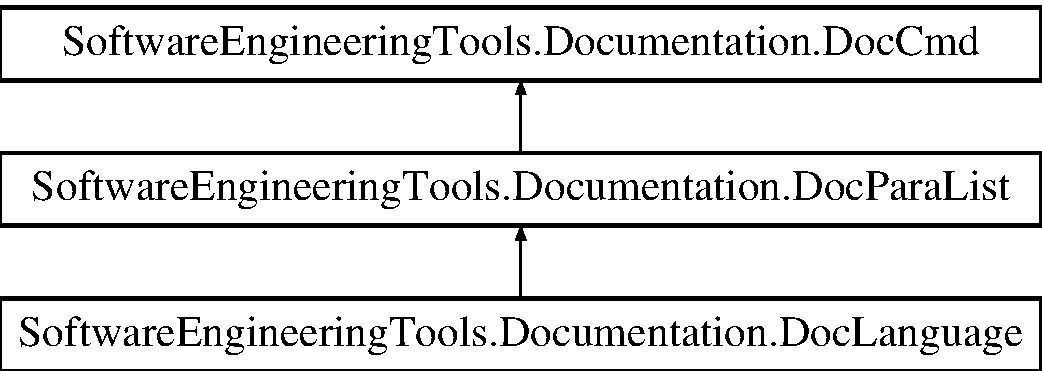
\includegraphics[height=3.000000cm]{class_software_engineering_tools_1_1_documentation_1_1_doc_language}
\end{center}
\end{figure}
\subsection*{Public Member Functions}
\begin{DoxyCompactItemize}
\item 
\hyperlink{class_software_engineering_tools_1_1_documentation_1_1_doc_language_a1eac6da5efa1b1b3713a527267cb1941}{Doc\+Language} ()
\end{DoxyCompactItemize}
\subsection*{Properties}
\begin{DoxyCompactItemize}
\item 
string \hyperlink{class_software_engineering_tools_1_1_documentation_1_1_doc_language_a2f72ea1497ef3060ceab4eb7f1b419fc}{Language\+Id}\hspace{0.3cm}{\ttfamily  \mbox{[}get, set\mbox{]}}
\end{DoxyCompactItemize}


\subsection{Detailed Description}


Definition at line 951 of file Doxygen.\+cs.



\subsection{Constructor \& Destructor Documentation}
\hypertarget{class_software_engineering_tools_1_1_documentation_1_1_doc_language_a1eac6da5efa1b1b3713a527267cb1941}{\index{Software\+Engineering\+Tools\+::\+Documentation\+::\+Doc\+Language@{Software\+Engineering\+Tools\+::\+Documentation\+::\+Doc\+Language}!Doc\+Language@{Doc\+Language}}
\index{Doc\+Language@{Doc\+Language}!Software\+Engineering\+Tools\+::\+Documentation\+::\+Doc\+Language@{Software\+Engineering\+Tools\+::\+Documentation\+::\+Doc\+Language}}
\subsubsection[{Doc\+Language}]{\setlength{\rightskip}{0pt plus 5cm}Software\+Engineering\+Tools.\+Documentation.\+Doc\+Language.\+Doc\+Language (
\begin{DoxyParamCaption}
{}
\end{DoxyParamCaption}
)}}\label{class_software_engineering_tools_1_1_documentation_1_1_doc_language_a1eac6da5efa1b1b3713a527267cb1941}


Definition at line 955 of file Doxygen.\+cs.



\subsection{Property Documentation}
\hypertarget{class_software_engineering_tools_1_1_documentation_1_1_doc_language_a2f72ea1497ef3060ceab4eb7f1b419fc}{\index{Software\+Engineering\+Tools\+::\+Documentation\+::\+Doc\+Language@{Software\+Engineering\+Tools\+::\+Documentation\+::\+Doc\+Language}!Language\+Id@{Language\+Id}}
\index{Language\+Id@{Language\+Id}!Software\+Engineering\+Tools\+::\+Documentation\+::\+Doc\+Language@{Software\+Engineering\+Tools\+::\+Documentation\+::\+Doc\+Language}}
\subsubsection[{Language\+Id}]{\setlength{\rightskip}{0pt plus 5cm}string Software\+Engineering\+Tools.\+Documentation.\+Doc\+Language.\+Language\+Id\hspace{0.3cm}{\ttfamily [get]}, {\ttfamily [set]}}}\label{class_software_engineering_tools_1_1_documentation_1_1_doc_language_a2f72ea1497ef3060ceab4eb7f1b419fc}


Definition at line 953 of file Doxygen.\+cs.



The documentation for this class was generated from the following file\+:\begin{DoxyCompactItemize}
\item 
Api\+Doc\+Lib/\hyperlink{_doxygen_8cs}{Doxygen.\+cs}\end{DoxyCompactItemize}

\hypertarget{class_software_engineering_tools_1_1_documentation_1_1_doc_list}{\section{Software\+Engineering\+Tools.\+Documentation.\+Doc\+List Class Reference}
\label{class_software_engineering_tools_1_1_documentation_1_1_doc_list}\index{Software\+Engineering\+Tools.\+Documentation.\+Doc\+List@{Software\+Engineering\+Tools.\+Documentation.\+Doc\+List}}
}
Inheritance diagram for Software\+Engineering\+Tools.\+Documentation.\+Doc\+List\+:\begin{figure}[H]
\begin{center}
\leavevmode
\includegraphics[height=2.000000cm]{class_software_engineering_tools_1_1_documentation_1_1_doc_list}
\end{center}
\end{figure}
\subsection*{Public Member Functions}
\begin{DoxyCompactItemize}
\item 
\hyperlink{class_software_engineering_tools_1_1_documentation_1_1_doc_list_ada45bf6b3763efd1412e2a0fe49f4547}{Doc\+List} ()
\end{DoxyCompactItemize}
\subsection*{Properties}
\begin{DoxyCompactItemize}
\item 
\hyperlink{namespace_software_engineering_tools_1_1_documentation_ae0bccf4f49a76db084c1c316e5954ec9a4ee29ca12c7d126654bd0e5275de6135}{List}$<$ \hyperlink{class_software_engineering_tools_1_1_documentation_1_1_doc_list_item}{Doc\+List\+Item} $>$ \hyperlink{class_software_engineering_tools_1_1_documentation_1_1_doc_list_ad3fed80c8386c62e26ce7915ff05340c}{Items}\hspace{0.3cm}{\ttfamily  \mbox{[}get, set\mbox{]}}
\end{DoxyCompactItemize}


\subsection{Detailed Description}


Definition at line 766 of file Doxygen.\+cs.



\subsection{Constructor \& Destructor Documentation}
\hypertarget{class_software_engineering_tools_1_1_documentation_1_1_doc_list_ada45bf6b3763efd1412e2a0fe49f4547}{\index{Software\+Engineering\+Tools\+::\+Documentation\+::\+Doc\+List@{Software\+Engineering\+Tools\+::\+Documentation\+::\+Doc\+List}!Doc\+List@{Doc\+List}}
\index{Doc\+List@{Doc\+List}!Software\+Engineering\+Tools\+::\+Documentation\+::\+Doc\+List@{Software\+Engineering\+Tools\+::\+Documentation\+::\+Doc\+List}}
\subsubsection[{Doc\+List}]{\setlength{\rightskip}{0pt plus 5cm}Software\+Engineering\+Tools.\+Documentation.\+Doc\+List.\+Doc\+List (
\begin{DoxyParamCaption}
{}
\end{DoxyParamCaption}
)}}\label{class_software_engineering_tools_1_1_documentation_1_1_doc_list_ada45bf6b3763efd1412e2a0fe49f4547}


Definition at line 770 of file Doxygen.\+cs.



\subsection{Property Documentation}
\hypertarget{class_software_engineering_tools_1_1_documentation_1_1_doc_list_ad3fed80c8386c62e26ce7915ff05340c}{\index{Software\+Engineering\+Tools\+::\+Documentation\+::\+Doc\+List@{Software\+Engineering\+Tools\+::\+Documentation\+::\+Doc\+List}!Items@{Items}}
\index{Items@{Items}!Software\+Engineering\+Tools\+::\+Documentation\+::\+Doc\+List@{Software\+Engineering\+Tools\+::\+Documentation\+::\+Doc\+List}}
\subsubsection[{Items}]{\setlength{\rightskip}{0pt plus 5cm}{\bf List}$<${\bf Doc\+List\+Item}$>$ Software\+Engineering\+Tools.\+Documentation.\+Doc\+List.\+Items\hspace{0.3cm}{\ttfamily [get]}, {\ttfamily [set]}}}\label{class_software_engineering_tools_1_1_documentation_1_1_doc_list_ad3fed80c8386c62e26ce7915ff05340c}


Definition at line 768 of file Doxygen.\+cs.



The documentation for this class was generated from the following file\+:\begin{DoxyCompactItemize}
\item 
Api\+Doc\+Lib/\hyperlink{_doxygen_8cs}{Doxygen.\+cs}\end{DoxyCompactItemize}

\hypertarget{class_software_engineering_tools_1_1_documentation_1_1_doc_list_item}{\section{Software\+Engineering\+Tools.\+Documentation.\+Doc\+List\+Item Class Reference}
\label{class_software_engineering_tools_1_1_documentation_1_1_doc_list_item}\index{Software\+Engineering\+Tools.\+Documentation.\+Doc\+List\+Item@{Software\+Engineering\+Tools.\+Documentation.\+Doc\+List\+Item}}
}
Inheritance diagram for Software\+Engineering\+Tools.\+Documentation.\+Doc\+List\+Item\+:\begin{figure}[H]
\begin{center}
\leavevmode
\includegraphics[height=3.000000cm]{class_software_engineering_tools_1_1_documentation_1_1_doc_list_item}
\end{center}
\end{figure}
\subsection*{Public Member Functions}
\begin{DoxyCompactItemize}
\item 
\hyperlink{class_software_engineering_tools_1_1_documentation_1_1_doc_list_item_ad174681536e6a05bef68c390cf7da8f9}{Doc\+List\+Item} ()
\end{DoxyCompactItemize}
\subsection*{Additional Inherited Members}


\subsection{Detailed Description}


Definition at line 777 of file Doxygen.\+cs.



\subsection{Constructor \& Destructor Documentation}
\hypertarget{class_software_engineering_tools_1_1_documentation_1_1_doc_list_item_ad174681536e6a05bef68c390cf7da8f9}{\index{Software\+Engineering\+Tools\+::\+Documentation\+::\+Doc\+List\+Item@{Software\+Engineering\+Tools\+::\+Documentation\+::\+Doc\+List\+Item}!Doc\+List\+Item@{Doc\+List\+Item}}
\index{Doc\+List\+Item@{Doc\+List\+Item}!Software\+Engineering\+Tools\+::\+Documentation\+::\+Doc\+List\+Item@{Software\+Engineering\+Tools\+::\+Documentation\+::\+Doc\+List\+Item}}
\subsubsection[{Doc\+List\+Item}]{\setlength{\rightskip}{0pt plus 5cm}Software\+Engineering\+Tools.\+Documentation.\+Doc\+List\+Item.\+Doc\+List\+Item (
\begin{DoxyParamCaption}
{}
\end{DoxyParamCaption}
)}}\label{class_software_engineering_tools_1_1_documentation_1_1_doc_list_item_ad174681536e6a05bef68c390cf7da8f9}


Definition at line 779 of file Doxygen.\+cs.



The documentation for this class was generated from the following file\+:\begin{DoxyCompactItemize}
\item 
Api\+Doc\+Lib/\hyperlink{_doxygen_8cs}{Doxygen.\+cs}\end{DoxyCompactItemize}

\hypertarget{class_software_engineering_tools_1_1_documentation_1_1_doc_markup}{\section{Software\+Engineering\+Tools.\+Documentation.\+Doc\+Markup Class Reference}
\label{class_software_engineering_tools_1_1_documentation_1_1_doc_markup}\index{Software\+Engineering\+Tools.\+Documentation.\+Doc\+Markup@{Software\+Engineering\+Tools.\+Documentation.\+Doc\+Markup}}
}
Inheritance diagram for Software\+Engineering\+Tools.\+Documentation.\+Doc\+Markup\+:\begin{figure}[H]
\begin{center}
\leavevmode
\includegraphics[height=3.000000cm]{class_software_engineering_tools_1_1_documentation_1_1_doc_markup}
\end{center}
\end{figure}
\subsection*{Public Member Functions}
\begin{DoxyCompactItemize}
\item 
\hyperlink{class_software_engineering_tools_1_1_documentation_1_1_doc_markup_a061378317e6be3bffeaf80970acb88f0}{Doc\+Markup} ()
\end{DoxyCompactItemize}
\subsection*{Properties}
\begin{DoxyCompactItemize}
\item 
\hyperlink{namespace_software_engineering_tools_1_1_documentation_aa3643086f24cd1d8ba619a3b0dbb183f}{Doc\+Markup\+Kind} \hyperlink{class_software_engineering_tools_1_1_documentation_1_1_doc_markup_aba8537f35f564d8ad7375e2bb736544d}{Markup\+Kind}\hspace{0.3cm}{\ttfamily  \mbox{[}get, set\mbox{]}}
\end{DoxyCompactItemize}


\subsection{Detailed Description}


Definition at line 542 of file Doxygen.\+cs.



\subsection{Constructor \& Destructor Documentation}
\hypertarget{class_software_engineering_tools_1_1_documentation_1_1_doc_markup_a061378317e6be3bffeaf80970acb88f0}{\index{Software\+Engineering\+Tools\+::\+Documentation\+::\+Doc\+Markup@{Software\+Engineering\+Tools\+::\+Documentation\+::\+Doc\+Markup}!Doc\+Markup@{Doc\+Markup}}
\index{Doc\+Markup@{Doc\+Markup}!Software\+Engineering\+Tools\+::\+Documentation\+::\+Doc\+Markup@{Software\+Engineering\+Tools\+::\+Documentation\+::\+Doc\+Markup}}
\subsubsection[{Doc\+Markup}]{\setlength{\rightskip}{0pt plus 5cm}Software\+Engineering\+Tools.\+Documentation.\+Doc\+Markup.\+Doc\+Markup (
\begin{DoxyParamCaption}
{}
\end{DoxyParamCaption}
)}}\label{class_software_engineering_tools_1_1_documentation_1_1_doc_markup_a061378317e6be3bffeaf80970acb88f0}


Definition at line 546 of file Doxygen.\+cs.



\subsection{Property Documentation}
\hypertarget{class_software_engineering_tools_1_1_documentation_1_1_doc_markup_aba8537f35f564d8ad7375e2bb736544d}{\index{Software\+Engineering\+Tools\+::\+Documentation\+::\+Doc\+Markup@{Software\+Engineering\+Tools\+::\+Documentation\+::\+Doc\+Markup}!Markup\+Kind@{Markup\+Kind}}
\index{Markup\+Kind@{Markup\+Kind}!Software\+Engineering\+Tools\+::\+Documentation\+::\+Doc\+Markup@{Software\+Engineering\+Tools\+::\+Documentation\+::\+Doc\+Markup}}
\subsubsection[{Markup\+Kind}]{\setlength{\rightskip}{0pt plus 5cm}{\bf Doc\+Markup\+Kind} Software\+Engineering\+Tools.\+Documentation.\+Doc\+Markup.\+Markup\+Kind\hspace{0.3cm}{\ttfamily [get]}, {\ttfamily [set]}}}\label{class_software_engineering_tools_1_1_documentation_1_1_doc_markup_aba8537f35f564d8ad7375e2bb736544d}


Definition at line 544 of file Doxygen.\+cs.



The documentation for this class was generated from the following file\+:\begin{DoxyCompactItemize}
\item 
Api\+Doc\+Lib/\hyperlink{_doxygen_8cs}{Doxygen.\+cs}\end{DoxyCompactItemize}

\hypertarget{class_software_engineering_tools_1_1_documentation_1_1_doc_para}{\section{Software\+Engineering\+Tools.\+Documentation.\+Doc\+Para Class Reference}
\label{class_software_engineering_tools_1_1_documentation_1_1_doc_para}\index{Software\+Engineering\+Tools.\+Documentation.\+Doc\+Para@{Software\+Engineering\+Tools.\+Documentation.\+Doc\+Para}}
}
Inheritance diagram for Software\+Engineering\+Tools.\+Documentation.\+Doc\+Para\+:\begin{figure}[H]
\begin{center}
\leavevmode
\includegraphics[height=3.000000cm]{class_software_engineering_tools_1_1_documentation_1_1_doc_para}
\end{center}
\end{figure}
\subsection*{Public Member Functions}
\begin{DoxyCompactItemize}
\item 
\hyperlink{class_software_engineering_tools_1_1_documentation_1_1_doc_para_af311f79854670eededd4fc6d7525882f}{Doc\+Para} ()
\end{DoxyCompactItemize}
\subsection*{Additional Inherited Members}


\subsection{Detailed Description}


Definition at line 523 of file Doxygen.\+cs.



\subsection{Constructor \& Destructor Documentation}
\hypertarget{class_software_engineering_tools_1_1_documentation_1_1_doc_para_af311f79854670eededd4fc6d7525882f}{\index{Software\+Engineering\+Tools\+::\+Documentation\+::\+Doc\+Para@{Software\+Engineering\+Tools\+::\+Documentation\+::\+Doc\+Para}!Doc\+Para@{Doc\+Para}}
\index{Doc\+Para@{Doc\+Para}!Software\+Engineering\+Tools\+::\+Documentation\+::\+Doc\+Para@{Software\+Engineering\+Tools\+::\+Documentation\+::\+Doc\+Para}}
\subsubsection[{Doc\+Para}]{\setlength{\rightskip}{0pt plus 5cm}Software\+Engineering\+Tools.\+Documentation.\+Doc\+Para.\+Doc\+Para (
\begin{DoxyParamCaption}
{}
\end{DoxyParamCaption}
)}}\label{class_software_engineering_tools_1_1_documentation_1_1_doc_para_af311f79854670eededd4fc6d7525882f}


Definition at line 525 of file Doxygen.\+cs.



The documentation for this class was generated from the following file\+:\begin{DoxyCompactItemize}
\item 
Api\+Doc\+Lib/\hyperlink{_doxygen_8cs}{Doxygen.\+cs}\end{DoxyCompactItemize}

\hypertarget{class_software_engineering_tools_1_1_documentation_1_1_doc_para_list}{\section{Software\+Engineering\+Tools.\+Documentation.\+Doc\+Para\+List Class Reference}
\label{class_software_engineering_tools_1_1_documentation_1_1_doc_para_list}\index{Software\+Engineering\+Tools.\+Documentation.\+Doc\+Para\+List@{Software\+Engineering\+Tools.\+Documentation.\+Doc\+Para\+List}}
}
Inheritance diagram for Software\+Engineering\+Tools.\+Documentation.\+Doc\+Para\+List\+:\begin{figure}[H]
\begin{center}
\leavevmode
\includegraphics[height=0.918033cm]{class_software_engineering_tools_1_1_documentation_1_1_doc_para_list}
\end{center}
\end{figure}
\subsection*{Public Member Functions}
\begin{DoxyCompactItemize}
\item 
\hyperlink{class_software_engineering_tools_1_1_documentation_1_1_doc_para_list_ad8dbbcf2c31cb83c1d32bda88f3aebe4}{Doc\+Para\+List} ()
\end{DoxyCompactItemize}
\subsection*{Properties}
\begin{DoxyCompactItemize}
\item 
\hyperlink{namespace_software_engineering_tools_1_1_documentation_ae0bccf4f49a76db084c1c316e5954ec9a4ee29ca12c7d126654bd0e5275de6135}{List}$<$ \hyperlink{class_software_engineering_tools_1_1_documentation_1_1_doc_para}{Doc\+Para} $>$ \hyperlink{class_software_engineering_tools_1_1_documentation_1_1_doc_para_list_a0758f3ee3b3bb618b24c793d66c00c3a}{Paragraphs}\hspace{0.3cm}{\ttfamily  \mbox{[}get, set\mbox{]}}
\end{DoxyCompactItemize}


\subsection{Detailed Description}


Definition at line 531 of file Doxygen.\+cs.



\subsection{Constructor \& Destructor Documentation}
\hypertarget{class_software_engineering_tools_1_1_documentation_1_1_doc_para_list_ad8dbbcf2c31cb83c1d32bda88f3aebe4}{\index{Software\+Engineering\+Tools\+::\+Documentation\+::\+Doc\+Para\+List@{Software\+Engineering\+Tools\+::\+Documentation\+::\+Doc\+Para\+List}!Doc\+Para\+List@{Doc\+Para\+List}}
\index{Doc\+Para\+List@{Doc\+Para\+List}!Software\+Engineering\+Tools\+::\+Documentation\+::\+Doc\+Para\+List@{Software\+Engineering\+Tools\+::\+Documentation\+::\+Doc\+Para\+List}}
\subsubsection[{Doc\+Para\+List}]{\setlength{\rightskip}{0pt plus 5cm}Software\+Engineering\+Tools.\+Documentation.\+Doc\+Para\+List.\+Doc\+Para\+List (
\begin{DoxyParamCaption}
{}
\end{DoxyParamCaption}
)}}\label{class_software_engineering_tools_1_1_documentation_1_1_doc_para_list_ad8dbbcf2c31cb83c1d32bda88f3aebe4}


Definition at line 535 of file Doxygen.\+cs.



\subsection{Property Documentation}
\hypertarget{class_software_engineering_tools_1_1_documentation_1_1_doc_para_list_a0758f3ee3b3bb618b24c793d66c00c3a}{\index{Software\+Engineering\+Tools\+::\+Documentation\+::\+Doc\+Para\+List@{Software\+Engineering\+Tools\+::\+Documentation\+::\+Doc\+Para\+List}!Paragraphs@{Paragraphs}}
\index{Paragraphs@{Paragraphs}!Software\+Engineering\+Tools\+::\+Documentation\+::\+Doc\+Para\+List@{Software\+Engineering\+Tools\+::\+Documentation\+::\+Doc\+Para\+List}}
\subsubsection[{Paragraphs}]{\setlength{\rightskip}{0pt plus 5cm}{\bf List}$<${\bf Doc\+Para}$>$ Software\+Engineering\+Tools.\+Documentation.\+Doc\+Para\+List.\+Paragraphs\hspace{0.3cm}{\ttfamily [get]}, {\ttfamily [set]}}}\label{class_software_engineering_tools_1_1_documentation_1_1_doc_para_list_a0758f3ee3b3bb618b24c793d66c00c3a}


Definition at line 533 of file Doxygen.\+cs.



The documentation for this class was generated from the following file\+:\begin{DoxyCompactItemize}
\item 
Api\+Doc\+Lib/\hyperlink{_doxygen_8cs}{Doxygen.\+cs}\end{DoxyCompactItemize}

\hypertarget{class_software_engineering_tools_1_1_documentation_1_1_doc_param_list}{\section{Software\+Engineering\+Tools.\+Documentation.\+Doc\+Param\+List Class Reference}
\label{class_software_engineering_tools_1_1_documentation_1_1_doc_param_list}\index{Software\+Engineering\+Tools.\+Documentation.\+Doc\+Param\+List@{Software\+Engineering\+Tools.\+Documentation.\+Doc\+Param\+List}}
}
Inheritance diagram for Software\+Engineering\+Tools.\+Documentation.\+Doc\+Param\+List\+:\begin{figure}[H]
\begin{center}
\leavevmode
\includegraphics[height=2.000000cm]{class_software_engineering_tools_1_1_documentation_1_1_doc_param_list}
\end{center}
\end{figure}
\subsection*{Public Member Functions}
\begin{DoxyCompactItemize}
\item 
\hyperlink{class_software_engineering_tools_1_1_documentation_1_1_doc_param_list_a73c7e9030279243ecf33ebb17cb5deb5}{Doc\+Param\+List} ()
\end{DoxyCompactItemize}
\subsection*{Properties}
\begin{DoxyCompactItemize}
\item 
\hyperlink{namespace_software_engineering_tools_1_1_documentation_a386ec98ace7dcc510b3dc1035c7bfb15}{Doc\+Param\+List\+Kind} \hyperlink{class_software_engineering_tools_1_1_documentation_1_1_doc_param_list_a83d72ccd96d99a45780852569978025b}{Param\+List\+Kind}\hspace{0.3cm}{\ttfamily  \mbox{[}get, set\mbox{]}}
\item 
\hyperlink{namespace_software_engineering_tools_1_1_documentation_ae0bccf4f49a76db084c1c316e5954ec9a4ee29ca12c7d126654bd0e5275de6135}{List}$<$ \hyperlink{class_software_engineering_tools_1_1_documentation_1_1_doc_param_list_item}{Doc\+Param\+List\+Item} $>$ \hyperlink{class_software_engineering_tools_1_1_documentation_1_1_doc_param_list_a2c0a39217a99edd79f005ee66acd3137}{Params}\hspace{0.3cm}{\ttfamily  \mbox{[}get, set\mbox{]}}
\end{DoxyCompactItemize}


\subsection{Detailed Description}


Definition at line 961 of file Doxygen.\+cs.



\subsection{Constructor \& Destructor Documentation}
\hypertarget{class_software_engineering_tools_1_1_documentation_1_1_doc_param_list_a73c7e9030279243ecf33ebb17cb5deb5}{\index{Software\+Engineering\+Tools\+::\+Documentation\+::\+Doc\+Param\+List@{Software\+Engineering\+Tools\+::\+Documentation\+::\+Doc\+Param\+List}!Doc\+Param\+List@{Doc\+Param\+List}}
\index{Doc\+Param\+List@{Doc\+Param\+List}!Software\+Engineering\+Tools\+::\+Documentation\+::\+Doc\+Param\+List@{Software\+Engineering\+Tools\+::\+Documentation\+::\+Doc\+Param\+List}}
\subsubsection[{Doc\+Param\+List}]{\setlength{\rightskip}{0pt plus 5cm}Software\+Engineering\+Tools.\+Documentation.\+Doc\+Param\+List.\+Doc\+Param\+List (
\begin{DoxyParamCaption}
{}
\end{DoxyParamCaption}
)}}\label{class_software_engineering_tools_1_1_documentation_1_1_doc_param_list_a73c7e9030279243ecf33ebb17cb5deb5}


Definition at line 966 of file Doxygen.\+cs.



\subsection{Property Documentation}
\hypertarget{class_software_engineering_tools_1_1_documentation_1_1_doc_param_list_a83d72ccd96d99a45780852569978025b}{\index{Software\+Engineering\+Tools\+::\+Documentation\+::\+Doc\+Param\+List@{Software\+Engineering\+Tools\+::\+Documentation\+::\+Doc\+Param\+List}!Param\+List\+Kind@{Param\+List\+Kind}}
\index{Param\+List\+Kind@{Param\+List\+Kind}!Software\+Engineering\+Tools\+::\+Documentation\+::\+Doc\+Param\+List@{Software\+Engineering\+Tools\+::\+Documentation\+::\+Doc\+Param\+List}}
\subsubsection[{Param\+List\+Kind}]{\setlength{\rightskip}{0pt plus 5cm}{\bf Doc\+Param\+List\+Kind} Software\+Engineering\+Tools.\+Documentation.\+Doc\+Param\+List.\+Param\+List\+Kind\hspace{0.3cm}{\ttfamily [get]}, {\ttfamily [set]}}}\label{class_software_engineering_tools_1_1_documentation_1_1_doc_param_list_a83d72ccd96d99a45780852569978025b}


Definition at line 963 of file Doxygen.\+cs.

\hypertarget{class_software_engineering_tools_1_1_documentation_1_1_doc_param_list_a2c0a39217a99edd79f005ee66acd3137}{\index{Software\+Engineering\+Tools\+::\+Documentation\+::\+Doc\+Param\+List@{Software\+Engineering\+Tools\+::\+Documentation\+::\+Doc\+Param\+List}!Params@{Params}}
\index{Params@{Params}!Software\+Engineering\+Tools\+::\+Documentation\+::\+Doc\+Param\+List@{Software\+Engineering\+Tools\+::\+Documentation\+::\+Doc\+Param\+List}}
\subsubsection[{Params}]{\setlength{\rightskip}{0pt plus 5cm}{\bf List}$<${\bf Doc\+Param\+List\+Item}$>$ Software\+Engineering\+Tools.\+Documentation.\+Doc\+Param\+List.\+Params\hspace{0.3cm}{\ttfamily [get]}, {\ttfamily [set]}}}\label{class_software_engineering_tools_1_1_documentation_1_1_doc_param_list_a2c0a39217a99edd79f005ee66acd3137}


Definition at line 964 of file Doxygen.\+cs.



The documentation for this class was generated from the following file\+:\begin{DoxyCompactItemize}
\item 
Api\+Doc\+Lib/\hyperlink{_doxygen_8cs}{Doxygen.\+cs}\end{DoxyCompactItemize}

\hypertarget{class_software_engineering_tools_1_1_documentation_1_1_doc_param_list_item}{\section{Software\+Engineering\+Tools.\+Documentation.\+Doc\+Param\+List\+Item Class Reference}
\label{class_software_engineering_tools_1_1_documentation_1_1_doc_param_list_item}\index{Software\+Engineering\+Tools.\+Documentation.\+Doc\+Param\+List\+Item@{Software\+Engineering\+Tools.\+Documentation.\+Doc\+Param\+List\+Item}}
}
\subsection*{Public Member Functions}
\begin{DoxyCompactItemize}
\item 
\hyperlink{class_software_engineering_tools_1_1_documentation_1_1_doc_param_list_item_a1c659976c8f26af3b73450a4a8a36997}{Doc\+Param\+List\+Item} ()
\end{DoxyCompactItemize}
\subsection*{Properties}
\begin{DoxyCompactItemize}
\item 
\hyperlink{namespace_software_engineering_tools_1_1_documentation_ae0bccf4f49a76db084c1c316e5954ec9a4ee29ca12c7d126654bd0e5275de6135}{List}$<$ \hyperlink{class_software_engineering_tools_1_1_documentation_1_1_doc_param_name_list}{Doc\+Param\+Name\+List} $>$ \hyperlink{class_software_engineering_tools_1_1_documentation_1_1_doc_param_list_item_ad01ae5f9eec5ea62d109669011cd1057}{Param\+Names}\hspace{0.3cm}{\ttfamily  \mbox{[}get, set\mbox{]}}
\item 
\hyperlink{class_software_engineering_tools_1_1_documentation_1_1_description}{Description} \hyperlink{class_software_engineering_tools_1_1_documentation_1_1_doc_param_list_item_a3a9c87ee0dd403127be13ef7b8d6579a}{Description}\hspace{0.3cm}{\ttfamily  \mbox{[}get, set\mbox{]}}
\end{DoxyCompactItemize}


\subsection{Detailed Description}


Definition at line 981 of file Doxygen.\+cs.



\subsection{Constructor \& Destructor Documentation}
\hypertarget{class_software_engineering_tools_1_1_documentation_1_1_doc_param_list_item_a1c659976c8f26af3b73450a4a8a36997}{\index{Software\+Engineering\+Tools\+::\+Documentation\+::\+Doc\+Param\+List\+Item@{Software\+Engineering\+Tools\+::\+Documentation\+::\+Doc\+Param\+List\+Item}!Doc\+Param\+List\+Item@{Doc\+Param\+List\+Item}}
\index{Doc\+Param\+List\+Item@{Doc\+Param\+List\+Item}!Software\+Engineering\+Tools\+::\+Documentation\+::\+Doc\+Param\+List\+Item@{Software\+Engineering\+Tools\+::\+Documentation\+::\+Doc\+Param\+List\+Item}}
\subsubsection[{Doc\+Param\+List\+Item}]{\setlength{\rightskip}{0pt plus 5cm}Software\+Engineering\+Tools.\+Documentation.\+Doc\+Param\+List\+Item.\+Doc\+Param\+List\+Item (
\begin{DoxyParamCaption}
{}
\end{DoxyParamCaption}
)}}\label{class_software_engineering_tools_1_1_documentation_1_1_doc_param_list_item_a1c659976c8f26af3b73450a4a8a36997}


Definition at line 986 of file Doxygen.\+cs.



\subsection{Property Documentation}
\hypertarget{class_software_engineering_tools_1_1_documentation_1_1_doc_param_list_item_a3a9c87ee0dd403127be13ef7b8d6579a}{\index{Software\+Engineering\+Tools\+::\+Documentation\+::\+Doc\+Param\+List\+Item@{Software\+Engineering\+Tools\+::\+Documentation\+::\+Doc\+Param\+List\+Item}!Description@{Description}}
\index{Description@{Description}!Software\+Engineering\+Tools\+::\+Documentation\+::\+Doc\+Param\+List\+Item@{Software\+Engineering\+Tools\+::\+Documentation\+::\+Doc\+Param\+List\+Item}}
\subsubsection[{Description}]{\setlength{\rightskip}{0pt plus 5cm}{\bf Description} Software\+Engineering\+Tools.\+Documentation.\+Doc\+Param\+List\+Item.\+Description\hspace{0.3cm}{\ttfamily [get]}, {\ttfamily [set]}}}\label{class_software_engineering_tools_1_1_documentation_1_1_doc_param_list_item_a3a9c87ee0dd403127be13ef7b8d6579a}


Definition at line 984 of file Doxygen.\+cs.

\hypertarget{class_software_engineering_tools_1_1_documentation_1_1_doc_param_list_item_ad01ae5f9eec5ea62d109669011cd1057}{\index{Software\+Engineering\+Tools\+::\+Documentation\+::\+Doc\+Param\+List\+Item@{Software\+Engineering\+Tools\+::\+Documentation\+::\+Doc\+Param\+List\+Item}!Param\+Names@{Param\+Names}}
\index{Param\+Names@{Param\+Names}!Software\+Engineering\+Tools\+::\+Documentation\+::\+Doc\+Param\+List\+Item@{Software\+Engineering\+Tools\+::\+Documentation\+::\+Doc\+Param\+List\+Item}}
\subsubsection[{Param\+Names}]{\setlength{\rightskip}{0pt plus 5cm}{\bf List}$<${\bf Doc\+Param\+Name\+List}$>$ Software\+Engineering\+Tools.\+Documentation.\+Doc\+Param\+List\+Item.\+Param\+Names\hspace{0.3cm}{\ttfamily [get]}, {\ttfamily [set]}}}\label{class_software_engineering_tools_1_1_documentation_1_1_doc_param_list_item_ad01ae5f9eec5ea62d109669011cd1057}


Definition at line 983 of file Doxygen.\+cs.



The documentation for this class was generated from the following file\+:\begin{DoxyCompactItemize}
\item 
Api\+Doc\+Lib/\hyperlink{_doxygen_8cs}{Doxygen.\+cs}\end{DoxyCompactItemize}

\hypertarget{class_software_engineering_tools_1_1_documentation_1_1_doc_param_name}{\section{Software\+Engineering\+Tools.\+Documentation.\+Doc\+Param\+Name Class Reference}
\label{class_software_engineering_tools_1_1_documentation_1_1_doc_param_name}\index{Software\+Engineering\+Tools.\+Documentation.\+Doc\+Param\+Name@{Software\+Engineering\+Tools.\+Documentation.\+Doc\+Param\+Name}}
}
\subsection*{Properties}
\begin{DoxyCompactItemize}
\item 
\hyperlink{class_software_engineering_tools_1_1_documentation_1_1_doc_reference}{Doc\+Reference} \hyperlink{class_software_engineering_tools_1_1_documentation_1_1_doc_param_name_ab7dec2f8730fe0d01e3e58ea7005ea2b}{Name}\hspace{0.3cm}{\ttfamily  \mbox{[}get, set\mbox{]}}
\item 
\hyperlink{namespace_software_engineering_tools_1_1_documentation_a1884fb8c74d10c2aa19068ac530df736}{Doc\+Param\+Dir} \hyperlink{class_software_engineering_tools_1_1_documentation_1_1_doc_param_name_a84eadb221dca0122ae106517972c7ad4}{Direction}\hspace{0.3cm}{\ttfamily  \mbox{[}get, set\mbox{]}}
\end{DoxyCompactItemize}


\subsection{Detailed Description}


Definition at line 1004 of file Doxygen.\+cs.



\subsection{Property Documentation}
\hypertarget{class_software_engineering_tools_1_1_documentation_1_1_doc_param_name_a84eadb221dca0122ae106517972c7ad4}{\index{Software\+Engineering\+Tools\+::\+Documentation\+::\+Doc\+Param\+Name@{Software\+Engineering\+Tools\+::\+Documentation\+::\+Doc\+Param\+Name}!Direction@{Direction}}
\index{Direction@{Direction}!Software\+Engineering\+Tools\+::\+Documentation\+::\+Doc\+Param\+Name@{Software\+Engineering\+Tools\+::\+Documentation\+::\+Doc\+Param\+Name}}
\subsubsection[{Direction}]{\setlength{\rightskip}{0pt plus 5cm}{\bf Doc\+Param\+Dir} Software\+Engineering\+Tools.\+Documentation.\+Doc\+Param\+Name.\+Direction\hspace{0.3cm}{\ttfamily [get]}, {\ttfamily [set]}}}\label{class_software_engineering_tools_1_1_documentation_1_1_doc_param_name_a84eadb221dca0122ae106517972c7ad4}


Definition at line 1007 of file Doxygen.\+cs.

\hypertarget{class_software_engineering_tools_1_1_documentation_1_1_doc_param_name_ab7dec2f8730fe0d01e3e58ea7005ea2b}{\index{Software\+Engineering\+Tools\+::\+Documentation\+::\+Doc\+Param\+Name@{Software\+Engineering\+Tools\+::\+Documentation\+::\+Doc\+Param\+Name}!Name@{Name}}
\index{Name@{Name}!Software\+Engineering\+Tools\+::\+Documentation\+::\+Doc\+Param\+Name@{Software\+Engineering\+Tools\+::\+Documentation\+::\+Doc\+Param\+Name}}
\subsubsection[{Name}]{\setlength{\rightskip}{0pt plus 5cm}{\bf Doc\+Reference} Software\+Engineering\+Tools.\+Documentation.\+Doc\+Param\+Name.\+Name\hspace{0.3cm}{\ttfamily [get]}, {\ttfamily [set]}}}\label{class_software_engineering_tools_1_1_documentation_1_1_doc_param_name_ab7dec2f8730fe0d01e3e58ea7005ea2b}


Definition at line 1006 of file Doxygen.\+cs.



The documentation for this class was generated from the following file\+:\begin{DoxyCompactItemize}
\item 
Api\+Doc\+Lib/\hyperlink{_doxygen_8cs}{Doxygen.\+cs}\end{DoxyCompactItemize}

\hypertarget{class_software_engineering_tools_1_1_documentation_1_1_doc_param_name_list}{\section{Software\+Engineering\+Tools.\+Documentation.\+Doc\+Param\+Name\+List Class Reference}
\label{class_software_engineering_tools_1_1_documentation_1_1_doc_param_name_list}\index{Software\+Engineering\+Tools.\+Documentation.\+Doc\+Param\+Name\+List@{Software\+Engineering\+Tools.\+Documentation.\+Doc\+Param\+Name\+List}}
}
\subsection*{Public Member Functions}
\begin{DoxyCompactItemize}
\item 
\hyperlink{class_software_engineering_tools_1_1_documentation_1_1_doc_param_name_list_aadacd4e56816fe6f8f7482c2d0dd45cc}{Doc\+Param\+Name\+List} ()
\end{DoxyCompactItemize}
\subsection*{Properties}
\begin{DoxyCompactItemize}
\item 
\hyperlink{namespace_software_engineering_tools_1_1_documentation_ae0bccf4f49a76db084c1c316e5954ec9a4ee29ca12c7d126654bd0e5275de6135}{List}$<$ \hyperlink{class_software_engineering_tools_1_1_documentation_1_1_doc_reference}{Doc\+Reference} $>$ \hyperlink{class_software_engineering_tools_1_1_documentation_1_1_doc_param_name_list_a75bc981d62487ee28dad2b03813142e5}{Types}\hspace{0.3cm}{\ttfamily  \mbox{[}get, set\mbox{]}}
\item 
\hyperlink{namespace_software_engineering_tools_1_1_documentation_ae0bccf4f49a76db084c1c316e5954ec9a4ee29ca12c7d126654bd0e5275de6135}{List}$<$ \hyperlink{class_software_engineering_tools_1_1_documentation_1_1_doc_param_name}{Doc\+Param\+Name} $>$ \hyperlink{class_software_engineering_tools_1_1_documentation_1_1_doc_param_name_list_aa90f33ac2bc4890276fd27b2c1fa8ddd}{Names}\hspace{0.3cm}{\ttfamily  \mbox{[}get, set\mbox{]}}
\end{DoxyCompactItemize}


\subsection{Detailed Description}


Definition at line 992 of file Doxygen.\+cs.



\subsection{Constructor \& Destructor Documentation}
\hypertarget{class_software_engineering_tools_1_1_documentation_1_1_doc_param_name_list_aadacd4e56816fe6f8f7482c2d0dd45cc}{\index{Software\+Engineering\+Tools\+::\+Documentation\+::\+Doc\+Param\+Name\+List@{Software\+Engineering\+Tools\+::\+Documentation\+::\+Doc\+Param\+Name\+List}!Doc\+Param\+Name\+List@{Doc\+Param\+Name\+List}}
\index{Doc\+Param\+Name\+List@{Doc\+Param\+Name\+List}!Software\+Engineering\+Tools\+::\+Documentation\+::\+Doc\+Param\+Name\+List@{Software\+Engineering\+Tools\+::\+Documentation\+::\+Doc\+Param\+Name\+List}}
\subsubsection[{Doc\+Param\+Name\+List}]{\setlength{\rightskip}{0pt plus 5cm}Software\+Engineering\+Tools.\+Documentation.\+Doc\+Param\+Name\+List.\+Doc\+Param\+Name\+List (
\begin{DoxyParamCaption}
{}
\end{DoxyParamCaption}
)}}\label{class_software_engineering_tools_1_1_documentation_1_1_doc_param_name_list_aadacd4e56816fe6f8f7482c2d0dd45cc}


Definition at line 997 of file Doxygen.\+cs.



\subsection{Property Documentation}
\hypertarget{class_software_engineering_tools_1_1_documentation_1_1_doc_param_name_list_aa90f33ac2bc4890276fd27b2c1fa8ddd}{\index{Software\+Engineering\+Tools\+::\+Documentation\+::\+Doc\+Param\+Name\+List@{Software\+Engineering\+Tools\+::\+Documentation\+::\+Doc\+Param\+Name\+List}!Names@{Names}}
\index{Names@{Names}!Software\+Engineering\+Tools\+::\+Documentation\+::\+Doc\+Param\+Name\+List@{Software\+Engineering\+Tools\+::\+Documentation\+::\+Doc\+Param\+Name\+List}}
\subsubsection[{Names}]{\setlength{\rightskip}{0pt plus 5cm}{\bf List}$<${\bf Doc\+Param\+Name}$>$ Software\+Engineering\+Tools.\+Documentation.\+Doc\+Param\+Name\+List.\+Names\hspace{0.3cm}{\ttfamily [get]}, {\ttfamily [set]}}}\label{class_software_engineering_tools_1_1_documentation_1_1_doc_param_name_list_aa90f33ac2bc4890276fd27b2c1fa8ddd}


Definition at line 995 of file Doxygen.\+cs.

\hypertarget{class_software_engineering_tools_1_1_documentation_1_1_doc_param_name_list_a75bc981d62487ee28dad2b03813142e5}{\index{Software\+Engineering\+Tools\+::\+Documentation\+::\+Doc\+Param\+Name\+List@{Software\+Engineering\+Tools\+::\+Documentation\+::\+Doc\+Param\+Name\+List}!Types@{Types}}
\index{Types@{Types}!Software\+Engineering\+Tools\+::\+Documentation\+::\+Doc\+Param\+Name\+List@{Software\+Engineering\+Tools\+::\+Documentation\+::\+Doc\+Param\+Name\+List}}
\subsubsection[{Types}]{\setlength{\rightskip}{0pt plus 5cm}{\bf List}$<${\bf Doc\+Reference}$>$ Software\+Engineering\+Tools.\+Documentation.\+Doc\+Param\+Name\+List.\+Types\hspace{0.3cm}{\ttfamily [get]}, {\ttfamily [set]}}}\label{class_software_engineering_tools_1_1_documentation_1_1_doc_param_name_list_a75bc981d62487ee28dad2b03813142e5}


Definition at line 994 of file Doxygen.\+cs.



The documentation for this class was generated from the following file\+:\begin{DoxyCompactItemize}
\item 
Api\+Doc\+Lib/\hyperlink{_doxygen_8cs}{Doxygen.\+cs}\end{DoxyCompactItemize}

\hypertarget{class_software_engineering_tools_1_1_documentation_1_1_doc_reference}{\section{Software\+Engineering\+Tools.\+Documentation.\+Doc\+Reference Class Reference}
\label{class_software_engineering_tools_1_1_documentation_1_1_doc_reference}\index{Software\+Engineering\+Tools.\+Documentation.\+Doc\+Reference@{Software\+Engineering\+Tools.\+Documentation.\+Doc\+Reference}}
}
Inheritance diagram for Software\+Engineering\+Tools.\+Documentation.\+Doc\+Reference\+:\begin{figure}[H]
\begin{center}
\leavevmode
\includegraphics[height=3.000000cm]{class_software_engineering_tools_1_1_documentation_1_1_doc_reference}
\end{center}
\end{figure}
\subsection*{Public Member Functions}
\begin{DoxyCompactItemize}
\item 
\hyperlink{class_software_engineering_tools_1_1_documentation_1_1_doc_reference_aff445cccc14cc2765824f67df8ea134a}{Doc\+Reference} ()
\end{DoxyCompactItemize}
\subsection*{Properties}
\begin{DoxyCompactItemize}
\item 
\hyperlink{class_software_engineering_tools_1_1_documentation_1_1_compound}{Compound} \hyperlink{class_software_engineering_tools_1_1_documentation_1_1_doc_reference_a694938b5ed042c68e220ba01e26bdaf0}{Compound}\hspace{0.3cm}{\ttfamily  \mbox{[}get, set\mbox{]}}
\item 
\hyperlink{class_software_engineering_tools_1_1_documentation_1_1_dox_member}{Dox\+Member} \hyperlink{class_software_engineering_tools_1_1_documentation_1_1_doc_reference_a87ba528136728274b6ace3fac8f4ac5f}{Member}\hspace{0.3cm}{\ttfamily  \mbox{[}get, set\mbox{]}}
\item 
\hyperlink{namespace_software_engineering_tools_1_1_documentation_adb41ca18779eed53175de394c3d2bb67}{Doc\+Ref\+Kind} \hyperlink{class_software_engineering_tools_1_1_documentation_1_1_doc_reference_afe29145068a009c2e58f661f69038169}{Ref\+Kind}\hspace{0.3cm}{\ttfamily  \mbox{[}get, set\mbox{]}}
\item 
bool \hyperlink{class_software_engineering_tools_1_1_documentation_1_1_doc_reference_a72107943dc98d2883e85b689994d7351}{External}\hspace{0.3cm}{\ttfamily  \mbox{[}get, set\mbox{]}}
\end{DoxyCompactItemize}


\subsection{Detailed Description}


Definition at line 736 of file Doxygen.\+cs.



\subsection{Constructor \& Destructor Documentation}
\hypertarget{class_software_engineering_tools_1_1_documentation_1_1_doc_reference_aff445cccc14cc2765824f67df8ea134a}{\index{Software\+Engineering\+Tools\+::\+Documentation\+::\+Doc\+Reference@{Software\+Engineering\+Tools\+::\+Documentation\+::\+Doc\+Reference}!Doc\+Reference@{Doc\+Reference}}
\index{Doc\+Reference@{Doc\+Reference}!Software\+Engineering\+Tools\+::\+Documentation\+::\+Doc\+Reference@{Software\+Engineering\+Tools\+::\+Documentation\+::\+Doc\+Reference}}
\subsubsection[{Doc\+Reference}]{\setlength{\rightskip}{0pt plus 5cm}Software\+Engineering\+Tools.\+Documentation.\+Doc\+Reference.\+Doc\+Reference (
\begin{DoxyParamCaption}
{}
\end{DoxyParamCaption}
)}}\label{class_software_engineering_tools_1_1_documentation_1_1_doc_reference_aff445cccc14cc2765824f67df8ea134a}


Definition at line 743 of file Doxygen.\+cs.



\subsection{Property Documentation}
\hypertarget{class_software_engineering_tools_1_1_documentation_1_1_doc_reference_a694938b5ed042c68e220ba01e26bdaf0}{\index{Software\+Engineering\+Tools\+::\+Documentation\+::\+Doc\+Reference@{Software\+Engineering\+Tools\+::\+Documentation\+::\+Doc\+Reference}!Compound@{Compound}}
\index{Compound@{Compound}!Software\+Engineering\+Tools\+::\+Documentation\+::\+Doc\+Reference@{Software\+Engineering\+Tools\+::\+Documentation\+::\+Doc\+Reference}}
\subsubsection[{Compound}]{\setlength{\rightskip}{0pt plus 5cm}{\bf Compound} Software\+Engineering\+Tools.\+Documentation.\+Doc\+Reference.\+Compound\hspace{0.3cm}{\ttfamily [get]}, {\ttfamily [set]}}}\label{class_software_engineering_tools_1_1_documentation_1_1_doc_reference_a694938b5ed042c68e220ba01e26bdaf0}


Definition at line 738 of file Doxygen.\+cs.

\hypertarget{class_software_engineering_tools_1_1_documentation_1_1_doc_reference_a72107943dc98d2883e85b689994d7351}{\index{Software\+Engineering\+Tools\+::\+Documentation\+::\+Doc\+Reference@{Software\+Engineering\+Tools\+::\+Documentation\+::\+Doc\+Reference}!External@{External}}
\index{External@{External}!Software\+Engineering\+Tools\+::\+Documentation\+::\+Doc\+Reference@{Software\+Engineering\+Tools\+::\+Documentation\+::\+Doc\+Reference}}
\subsubsection[{External}]{\setlength{\rightskip}{0pt plus 5cm}bool Software\+Engineering\+Tools.\+Documentation.\+Doc\+Reference.\+External\hspace{0.3cm}{\ttfamily [get]}, {\ttfamily [set]}}}\label{class_software_engineering_tools_1_1_documentation_1_1_doc_reference_a72107943dc98d2883e85b689994d7351}


Definition at line 741 of file Doxygen.\+cs.

\hypertarget{class_software_engineering_tools_1_1_documentation_1_1_doc_reference_a87ba528136728274b6ace3fac8f4ac5f}{\index{Software\+Engineering\+Tools\+::\+Documentation\+::\+Doc\+Reference@{Software\+Engineering\+Tools\+::\+Documentation\+::\+Doc\+Reference}!Member@{Member}}
\index{Member@{Member}!Software\+Engineering\+Tools\+::\+Documentation\+::\+Doc\+Reference@{Software\+Engineering\+Tools\+::\+Documentation\+::\+Doc\+Reference}}
\subsubsection[{Member}]{\setlength{\rightskip}{0pt plus 5cm}{\bf Dox\+Member} Software\+Engineering\+Tools.\+Documentation.\+Doc\+Reference.\+Member\hspace{0.3cm}{\ttfamily [get]}, {\ttfamily [set]}}}\label{class_software_engineering_tools_1_1_documentation_1_1_doc_reference_a87ba528136728274b6ace3fac8f4ac5f}


Definition at line 739 of file Doxygen.\+cs.

\hypertarget{class_software_engineering_tools_1_1_documentation_1_1_doc_reference_afe29145068a009c2e58f661f69038169}{\index{Software\+Engineering\+Tools\+::\+Documentation\+::\+Doc\+Reference@{Software\+Engineering\+Tools\+::\+Documentation\+::\+Doc\+Reference}!Ref\+Kind@{Ref\+Kind}}
\index{Ref\+Kind@{Ref\+Kind}!Software\+Engineering\+Tools\+::\+Documentation\+::\+Doc\+Reference@{Software\+Engineering\+Tools\+::\+Documentation\+::\+Doc\+Reference}}
\subsubsection[{Ref\+Kind}]{\setlength{\rightskip}{0pt plus 5cm}{\bf Doc\+Ref\+Kind} Software\+Engineering\+Tools.\+Documentation.\+Doc\+Reference.\+Ref\+Kind\hspace{0.3cm}{\ttfamily [get]}, {\ttfamily [set]}}}\label{class_software_engineering_tools_1_1_documentation_1_1_doc_reference_afe29145068a009c2e58f661f69038169}


Definition at line 740 of file Doxygen.\+cs.



The documentation for this class was generated from the following file\+:\begin{DoxyCompactItemize}
\item 
Api\+Doc\+Lib/\hyperlink{_doxygen_8cs}{Doxygen.\+cs}\end{DoxyCompactItemize}

\hypertarget{class_software_engineering_tools_1_1_documentation_1_1_doc_sect}{\section{Software\+Engineering\+Tools.\+Documentation.\+Doc\+Sect Class Reference}
\label{class_software_engineering_tools_1_1_documentation_1_1_doc_sect}\index{Software\+Engineering\+Tools.\+Documentation.\+Doc\+Sect@{Software\+Engineering\+Tools.\+Documentation.\+Doc\+Sect}}
}
Inheritance diagram for Software\+Engineering\+Tools.\+Documentation.\+Doc\+Sect\+:\begin{figure}[H]
\begin{center}
\leavevmode
\includegraphics[height=4.000000cm]{class_software_engineering_tools_1_1_documentation_1_1_doc_sect}
\end{center}
\end{figure}
\subsection*{Public Member Functions}
\begin{DoxyCompactItemize}
\item 
\hyperlink{class_software_engineering_tools_1_1_documentation_1_1_doc_sect_adce39a3ebfcb0efa91ee3995bd1d022f}{Doc\+Sect} ()
\end{DoxyCompactItemize}
\subsection*{Properties}
\begin{DoxyCompactItemize}
\item 
string \hyperlink{class_software_engineering_tools_1_1_documentation_1_1_doc_sect_af51ffb6e3c0c2d2bad7cfdf4f04895a9}{Identifier}\hspace{0.3cm}{\ttfamily  \mbox{[}get, set\mbox{]}}
\end{DoxyCompactItemize}


\subsection{Detailed Description}


Definition at line 455 of file Doxygen.\+cs.



\subsection{Constructor \& Destructor Documentation}
\hypertarget{class_software_engineering_tools_1_1_documentation_1_1_doc_sect_adce39a3ebfcb0efa91ee3995bd1d022f}{\index{Software\+Engineering\+Tools\+::\+Documentation\+::\+Doc\+Sect@{Software\+Engineering\+Tools\+::\+Documentation\+::\+Doc\+Sect}!Doc\+Sect@{Doc\+Sect}}
\index{Doc\+Sect@{Doc\+Sect}!Software\+Engineering\+Tools\+::\+Documentation\+::\+Doc\+Sect@{Software\+Engineering\+Tools\+::\+Documentation\+::\+Doc\+Sect}}
\subsubsection[{Doc\+Sect}]{\setlength{\rightskip}{0pt plus 5cm}Software\+Engineering\+Tools.\+Documentation.\+Doc\+Sect.\+Doc\+Sect (
\begin{DoxyParamCaption}
{}
\end{DoxyParamCaption}
)}}\label{class_software_engineering_tools_1_1_documentation_1_1_doc_sect_adce39a3ebfcb0efa91ee3995bd1d022f}


Definition at line 459 of file Doxygen.\+cs.



\subsection{Property Documentation}
\hypertarget{class_software_engineering_tools_1_1_documentation_1_1_doc_sect_af51ffb6e3c0c2d2bad7cfdf4f04895a9}{\index{Software\+Engineering\+Tools\+::\+Documentation\+::\+Doc\+Sect@{Software\+Engineering\+Tools\+::\+Documentation\+::\+Doc\+Sect}!Identifier@{Identifier}}
\index{Identifier@{Identifier}!Software\+Engineering\+Tools\+::\+Documentation\+::\+Doc\+Sect@{Software\+Engineering\+Tools\+::\+Documentation\+::\+Doc\+Sect}}
\subsubsection[{Identifier}]{\setlength{\rightskip}{0pt plus 5cm}string Software\+Engineering\+Tools.\+Documentation.\+Doc\+Sect.\+Identifier\hspace{0.3cm}{\ttfamily [get]}, {\ttfamily [set]}}}\label{class_software_engineering_tools_1_1_documentation_1_1_doc_sect_af51ffb6e3c0c2d2bad7cfdf4f04895a9}


Definition at line 457 of file Doxygen.\+cs.



The documentation for this class was generated from the following file\+:\begin{DoxyCompactItemize}
\item 
Api\+Doc\+Lib/\hyperlink{_doxygen_8cs}{Doxygen.\+cs}\end{DoxyCompactItemize}

\hypertarget{class_software_engineering_tools_1_1_documentation_1_1_doc_simple_sect}{\section{Software\+Engineering\+Tools.\+Documentation.\+Doc\+Simple\+Sect Class Reference}
\label{class_software_engineering_tools_1_1_documentation_1_1_doc_simple_sect}\index{Software\+Engineering\+Tools.\+Documentation.\+Doc\+Simple\+Sect@{Software\+Engineering\+Tools.\+Documentation.\+Doc\+Simple\+Sect}}
}
Inheritance diagram for Software\+Engineering\+Tools.\+Documentation.\+Doc\+Simple\+Sect\+:\begin{figure}[H]
\begin{center}
\leavevmode
\includegraphics[height=2.000000cm]{class_software_engineering_tools_1_1_documentation_1_1_doc_simple_sect}
\end{center}
\end{figure}
\subsection*{Public Member Functions}
\begin{DoxyCompactItemize}
\item 
\hyperlink{class_software_engineering_tools_1_1_documentation_1_1_doc_simple_sect_a0a6d8e79010d9e03c6319fef6e08aff7}{Doc\+Simple\+Sect} ()
\end{DoxyCompactItemize}
\subsection*{Properties}
\begin{DoxyCompactItemize}
\item 
\hyperlink{namespace_software_engineering_tools_1_1_documentation_afbf354018df4b51c4b26a5cd7182555d}{Doc\+Simple\+Sect\+Kind} \hyperlink{class_software_engineering_tools_1_1_documentation_1_1_doc_simple_sect_a6a4b4036b16ccfb60f48c5e7df50ac40}{Simple\+Sect\+Kind}\hspace{0.3cm}{\ttfamily  \mbox{[}get, set\mbox{]}}
\item 
string \hyperlink{class_software_engineering_tools_1_1_documentation_1_1_doc_simple_sect_a1315d0d038a955a9ba38da4d299f05e2}{Title}\hspace{0.3cm}{\ttfamily  \mbox{[}get, set\mbox{]}}
\item 
\hyperlink{namespace_software_engineering_tools_1_1_documentation_ae0bccf4f49a76db084c1c316e5954ec9a4ee29ca12c7d126654bd0e5275de6135}{List}$<$ \hyperlink{class_software_engineering_tools_1_1_documentation_1_1_doc_simple_sect_item}{Doc\+Simple\+Sect\+Item} $>$ \hyperlink{class_software_engineering_tools_1_1_documentation_1_1_doc_simple_sect_ab7d54f32f51a5ee11242cd37f1bd39dc}{Items}\hspace{0.3cm}{\ttfamily  \mbox{[}get, set\mbox{]}}
\end{DoxyCompactItemize}


\subsection{Detailed Description}


Definition at line 785 of file Doxygen.\+cs.



\subsection{Constructor \& Destructor Documentation}
\hypertarget{class_software_engineering_tools_1_1_documentation_1_1_doc_simple_sect_a0a6d8e79010d9e03c6319fef6e08aff7}{\index{Software\+Engineering\+Tools\+::\+Documentation\+::\+Doc\+Simple\+Sect@{Software\+Engineering\+Tools\+::\+Documentation\+::\+Doc\+Simple\+Sect}!Doc\+Simple\+Sect@{Doc\+Simple\+Sect}}
\index{Doc\+Simple\+Sect@{Doc\+Simple\+Sect}!Software\+Engineering\+Tools\+::\+Documentation\+::\+Doc\+Simple\+Sect@{Software\+Engineering\+Tools\+::\+Documentation\+::\+Doc\+Simple\+Sect}}
\subsubsection[{Doc\+Simple\+Sect}]{\setlength{\rightskip}{0pt plus 5cm}Software\+Engineering\+Tools.\+Documentation.\+Doc\+Simple\+Sect.\+Doc\+Simple\+Sect (
\begin{DoxyParamCaption}
{}
\end{DoxyParamCaption}
)}}\label{class_software_engineering_tools_1_1_documentation_1_1_doc_simple_sect_a0a6d8e79010d9e03c6319fef6e08aff7}


Definition at line 791 of file Doxygen.\+cs.



\subsection{Property Documentation}
\hypertarget{class_software_engineering_tools_1_1_documentation_1_1_doc_simple_sect_ab7d54f32f51a5ee11242cd37f1bd39dc}{\index{Software\+Engineering\+Tools\+::\+Documentation\+::\+Doc\+Simple\+Sect@{Software\+Engineering\+Tools\+::\+Documentation\+::\+Doc\+Simple\+Sect}!Items@{Items}}
\index{Items@{Items}!Software\+Engineering\+Tools\+::\+Documentation\+::\+Doc\+Simple\+Sect@{Software\+Engineering\+Tools\+::\+Documentation\+::\+Doc\+Simple\+Sect}}
\subsubsection[{Items}]{\setlength{\rightskip}{0pt plus 5cm}{\bf List}$<${\bf Doc\+Simple\+Sect\+Item}$>$ Software\+Engineering\+Tools.\+Documentation.\+Doc\+Simple\+Sect.\+Items\hspace{0.3cm}{\ttfamily [get]}, {\ttfamily [set]}}}\label{class_software_engineering_tools_1_1_documentation_1_1_doc_simple_sect_ab7d54f32f51a5ee11242cd37f1bd39dc}


Definition at line 789 of file Doxygen.\+cs.

\hypertarget{class_software_engineering_tools_1_1_documentation_1_1_doc_simple_sect_a6a4b4036b16ccfb60f48c5e7df50ac40}{\index{Software\+Engineering\+Tools\+::\+Documentation\+::\+Doc\+Simple\+Sect@{Software\+Engineering\+Tools\+::\+Documentation\+::\+Doc\+Simple\+Sect}!Simple\+Sect\+Kind@{Simple\+Sect\+Kind}}
\index{Simple\+Sect\+Kind@{Simple\+Sect\+Kind}!Software\+Engineering\+Tools\+::\+Documentation\+::\+Doc\+Simple\+Sect@{Software\+Engineering\+Tools\+::\+Documentation\+::\+Doc\+Simple\+Sect}}
\subsubsection[{Simple\+Sect\+Kind}]{\setlength{\rightskip}{0pt plus 5cm}{\bf Doc\+Simple\+Sect\+Kind} Software\+Engineering\+Tools.\+Documentation.\+Doc\+Simple\+Sect.\+Simple\+Sect\+Kind\hspace{0.3cm}{\ttfamily [get]}, {\ttfamily [set]}}}\label{class_software_engineering_tools_1_1_documentation_1_1_doc_simple_sect_a6a4b4036b16ccfb60f48c5e7df50ac40}


Definition at line 787 of file Doxygen.\+cs.

\hypertarget{class_software_engineering_tools_1_1_documentation_1_1_doc_simple_sect_a1315d0d038a955a9ba38da4d299f05e2}{\index{Software\+Engineering\+Tools\+::\+Documentation\+::\+Doc\+Simple\+Sect@{Software\+Engineering\+Tools\+::\+Documentation\+::\+Doc\+Simple\+Sect}!Title@{Title}}
\index{Title@{Title}!Software\+Engineering\+Tools\+::\+Documentation\+::\+Doc\+Simple\+Sect@{Software\+Engineering\+Tools\+::\+Documentation\+::\+Doc\+Simple\+Sect}}
\subsubsection[{Title}]{\setlength{\rightskip}{0pt plus 5cm}string Software\+Engineering\+Tools.\+Documentation.\+Doc\+Simple\+Sect.\+Title\hspace{0.3cm}{\ttfamily [get]}, {\ttfamily [set]}}}\label{class_software_engineering_tools_1_1_documentation_1_1_doc_simple_sect_a1315d0d038a955a9ba38da4d299f05e2}


Definition at line 788 of file Doxygen.\+cs.



The documentation for this class was generated from the following file\+:\begin{DoxyCompactItemize}
\item 
Api\+Doc\+Lib/\hyperlink{_doxygen_8cs}{Doxygen.\+cs}\end{DoxyCompactItemize}

\hypertarget{class_software_engineering_tools_1_1_documentation_1_1_doc_simple_sect_item}{\section{Software\+Engineering\+Tools.\+Documentation.\+Doc\+Simple\+Sect\+Item Class Reference}
\label{class_software_engineering_tools_1_1_documentation_1_1_doc_simple_sect_item}\index{Software\+Engineering\+Tools.\+Documentation.\+Doc\+Simple\+Sect\+Item@{Software\+Engineering\+Tools.\+Documentation.\+Doc\+Simple\+Sect\+Item}}
}
Inheritance diagram for Software\+Engineering\+Tools.\+Documentation.\+Doc\+Simple\+Sect\+Item\+:\begin{figure}[H]
\begin{center}
\leavevmode
\includegraphics[height=3.000000cm]{class_software_engineering_tools_1_1_documentation_1_1_doc_simple_sect_item}
\end{center}
\end{figure}
\subsection*{Public Member Functions}
\begin{DoxyCompactItemize}
\item 
\hyperlink{class_software_engineering_tools_1_1_documentation_1_1_doc_simple_sect_item_a51b27f8b6bddfb9e1d74e3f74277adeb}{Doc\+Simple\+Sect\+Item} ()
\end{DoxyCompactItemize}
\subsection*{Properties}
\begin{DoxyCompactItemize}
\item 
\hyperlink{class_software_engineering_tools_1_1_documentation_1_1_doc_empty}{Doc\+Empty} \hyperlink{class_software_engineering_tools_1_1_documentation_1_1_doc_simple_sect_item_a04d97114512172cc8c9ac350582c8c22}{Separator}\hspace{0.3cm}{\ttfamily  \mbox{[}get, set\mbox{]}}
\end{DoxyCompactItemize}


\subsection{Detailed Description}


Definition at line 818 of file Doxygen.\+cs.



\subsection{Constructor \& Destructor Documentation}
\hypertarget{class_software_engineering_tools_1_1_documentation_1_1_doc_simple_sect_item_a51b27f8b6bddfb9e1d74e3f74277adeb}{\index{Software\+Engineering\+Tools\+::\+Documentation\+::\+Doc\+Simple\+Sect\+Item@{Software\+Engineering\+Tools\+::\+Documentation\+::\+Doc\+Simple\+Sect\+Item}!Doc\+Simple\+Sect\+Item@{Doc\+Simple\+Sect\+Item}}
\index{Doc\+Simple\+Sect\+Item@{Doc\+Simple\+Sect\+Item}!Software\+Engineering\+Tools\+::\+Documentation\+::\+Doc\+Simple\+Sect\+Item@{Software\+Engineering\+Tools\+::\+Documentation\+::\+Doc\+Simple\+Sect\+Item}}
\subsubsection[{Doc\+Simple\+Sect\+Item}]{\setlength{\rightskip}{0pt plus 5cm}Software\+Engineering\+Tools.\+Documentation.\+Doc\+Simple\+Sect\+Item.\+Doc\+Simple\+Sect\+Item (
\begin{DoxyParamCaption}
{}
\end{DoxyParamCaption}
)}}\label{class_software_engineering_tools_1_1_documentation_1_1_doc_simple_sect_item_a51b27f8b6bddfb9e1d74e3f74277adeb}


Definition at line 822 of file Doxygen.\+cs.



\subsection{Property Documentation}
\hypertarget{class_software_engineering_tools_1_1_documentation_1_1_doc_simple_sect_item_a04d97114512172cc8c9ac350582c8c22}{\index{Software\+Engineering\+Tools\+::\+Documentation\+::\+Doc\+Simple\+Sect\+Item@{Software\+Engineering\+Tools\+::\+Documentation\+::\+Doc\+Simple\+Sect\+Item}!Separator@{Separator}}
\index{Separator@{Separator}!Software\+Engineering\+Tools\+::\+Documentation\+::\+Doc\+Simple\+Sect\+Item@{Software\+Engineering\+Tools\+::\+Documentation\+::\+Doc\+Simple\+Sect\+Item}}
\subsubsection[{Separator}]{\setlength{\rightskip}{0pt plus 5cm}{\bf Doc\+Empty} Software\+Engineering\+Tools.\+Documentation.\+Doc\+Simple\+Sect\+Item.\+Separator\hspace{0.3cm}{\ttfamily [get]}, {\ttfamily [set]}}}\label{class_software_engineering_tools_1_1_documentation_1_1_doc_simple_sect_item_a04d97114512172cc8c9ac350582c8c22}


Definition at line 820 of file Doxygen.\+cs.



The documentation for this class was generated from the following file\+:\begin{DoxyCompactItemize}
\item 
Api\+Doc\+Lib/\hyperlink{_doxygen_8cs}{Doxygen.\+cs}\end{DoxyCompactItemize}

\hypertarget{class_software_engineering_tools_1_1_documentation_1_1_doc_table}{\section{Software\+Engineering\+Tools.\+Documentation.\+Doc\+Table Class Reference}
\label{class_software_engineering_tools_1_1_documentation_1_1_doc_table}\index{Software\+Engineering\+Tools.\+Documentation.\+Doc\+Table@{Software\+Engineering\+Tools.\+Documentation.\+Doc\+Table}}
}
Inheritance diagram for Software\+Engineering\+Tools.\+Documentation.\+Doc\+Table\+:\begin{figure}[H]
\begin{center}
\leavevmode
\includegraphics[height=2.000000cm]{class_software_engineering_tools_1_1_documentation_1_1_doc_table}
\end{center}
\end{figure}
\subsection*{Public Member Functions}
\begin{DoxyCompactItemize}
\item 
\hyperlink{class_software_engineering_tools_1_1_documentation_1_1_doc_table_a834a37e8969331cf2b37a442724b47c8}{Doc\+Table} ()
\end{DoxyCompactItemize}
\subsection*{Properties}
\begin{DoxyCompactItemize}
\item 
\hyperlink{namespace_software_engineering_tools_1_1_documentation_a4a8017aa254d1d05b03db5132b7dd3a7afa7153f7ed1cb6c0fcf2ffb2fac21748}{int} \hyperlink{class_software_engineering_tools_1_1_documentation_1_1_doc_table_a3cacca0fb8c937d9de2c1e9f9527af0e}{Row\+Count}\hspace{0.3cm}{\ttfamily  \mbox{[}get, set\mbox{]}}
\item 
\hyperlink{namespace_software_engineering_tools_1_1_documentation_a4a8017aa254d1d05b03db5132b7dd3a7afa7153f7ed1cb6c0fcf2ffb2fac21748}{int} \hyperlink{class_software_engineering_tools_1_1_documentation_1_1_doc_table_a66bdd113fc822da038a8aa8b5268436d}{Col\+Count}\hspace{0.3cm}{\ttfamily  \mbox{[}get, set\mbox{]}}
\item 
\hyperlink{class_software_engineering_tools_1_1_documentation_1_1_doc_caption}{Doc\+Caption} \hyperlink{class_software_engineering_tools_1_1_documentation_1_1_doc_table_ab394c3a4a562c8e1fc14ba15181c0a17}{Caption}\hspace{0.3cm}{\ttfamily  \mbox{[}get, set\mbox{]}}
\item 
\hyperlink{namespace_software_engineering_tools_1_1_documentation_ae0bccf4f49a76db084c1c316e5954ec9a4ee29ca12c7d126654bd0e5275de6135}{List}$<$ \hyperlink{class_software_engineering_tools_1_1_documentation_1_1_doc_table_row}{Doc\+Table\+Row} $>$ \hyperlink{class_software_engineering_tools_1_1_documentation_1_1_doc_table_a5da78858e249a4869f87f771bb2c50cf}{Rows}\hspace{0.3cm}{\ttfamily  \mbox{[}get, set\mbox{]}}
\end{DoxyCompactItemize}


\subsection{Detailed Description}


Definition at line 871 of file Doxygen.\+cs.



\subsection{Constructor \& Destructor Documentation}
\hypertarget{class_software_engineering_tools_1_1_documentation_1_1_doc_table_a834a37e8969331cf2b37a442724b47c8}{\index{Software\+Engineering\+Tools\+::\+Documentation\+::\+Doc\+Table@{Software\+Engineering\+Tools\+::\+Documentation\+::\+Doc\+Table}!Doc\+Table@{Doc\+Table}}
\index{Doc\+Table@{Doc\+Table}!Software\+Engineering\+Tools\+::\+Documentation\+::\+Doc\+Table@{Software\+Engineering\+Tools\+::\+Documentation\+::\+Doc\+Table}}
\subsubsection[{Doc\+Table}]{\setlength{\rightskip}{0pt plus 5cm}Software\+Engineering\+Tools.\+Documentation.\+Doc\+Table.\+Doc\+Table (
\begin{DoxyParamCaption}
{}
\end{DoxyParamCaption}
)}}\label{class_software_engineering_tools_1_1_documentation_1_1_doc_table_a834a37e8969331cf2b37a442724b47c8}


Definition at line 878 of file Doxygen.\+cs.



\subsection{Property Documentation}
\hypertarget{class_software_engineering_tools_1_1_documentation_1_1_doc_table_ab394c3a4a562c8e1fc14ba15181c0a17}{\index{Software\+Engineering\+Tools\+::\+Documentation\+::\+Doc\+Table@{Software\+Engineering\+Tools\+::\+Documentation\+::\+Doc\+Table}!Caption@{Caption}}
\index{Caption@{Caption}!Software\+Engineering\+Tools\+::\+Documentation\+::\+Doc\+Table@{Software\+Engineering\+Tools\+::\+Documentation\+::\+Doc\+Table}}
\subsubsection[{Caption}]{\setlength{\rightskip}{0pt plus 5cm}{\bf Doc\+Caption} Software\+Engineering\+Tools.\+Documentation.\+Doc\+Table.\+Caption\hspace{0.3cm}{\ttfamily [get]}, {\ttfamily [set]}}}\label{class_software_engineering_tools_1_1_documentation_1_1_doc_table_ab394c3a4a562c8e1fc14ba15181c0a17}


Definition at line 875 of file Doxygen.\+cs.

\hypertarget{class_software_engineering_tools_1_1_documentation_1_1_doc_table_a66bdd113fc822da038a8aa8b5268436d}{\index{Software\+Engineering\+Tools\+::\+Documentation\+::\+Doc\+Table@{Software\+Engineering\+Tools\+::\+Documentation\+::\+Doc\+Table}!Col\+Count@{Col\+Count}}
\index{Col\+Count@{Col\+Count}!Software\+Engineering\+Tools\+::\+Documentation\+::\+Doc\+Table@{Software\+Engineering\+Tools\+::\+Documentation\+::\+Doc\+Table}}
\subsubsection[{Col\+Count}]{\setlength{\rightskip}{0pt plus 5cm}{\bf int} Software\+Engineering\+Tools.\+Documentation.\+Doc\+Table.\+Col\+Count\hspace{0.3cm}{\ttfamily [get]}, {\ttfamily [set]}}}\label{class_software_engineering_tools_1_1_documentation_1_1_doc_table_a66bdd113fc822da038a8aa8b5268436d}


Definition at line 874 of file Doxygen.\+cs.

\hypertarget{class_software_engineering_tools_1_1_documentation_1_1_doc_table_a3cacca0fb8c937d9de2c1e9f9527af0e}{\index{Software\+Engineering\+Tools\+::\+Documentation\+::\+Doc\+Table@{Software\+Engineering\+Tools\+::\+Documentation\+::\+Doc\+Table}!Row\+Count@{Row\+Count}}
\index{Row\+Count@{Row\+Count}!Software\+Engineering\+Tools\+::\+Documentation\+::\+Doc\+Table@{Software\+Engineering\+Tools\+::\+Documentation\+::\+Doc\+Table}}
\subsubsection[{Row\+Count}]{\setlength{\rightskip}{0pt plus 5cm}{\bf int} Software\+Engineering\+Tools.\+Documentation.\+Doc\+Table.\+Row\+Count\hspace{0.3cm}{\ttfamily [get]}, {\ttfamily [set]}}}\label{class_software_engineering_tools_1_1_documentation_1_1_doc_table_a3cacca0fb8c937d9de2c1e9f9527af0e}


Definition at line 873 of file Doxygen.\+cs.

\hypertarget{class_software_engineering_tools_1_1_documentation_1_1_doc_table_a5da78858e249a4869f87f771bb2c50cf}{\index{Software\+Engineering\+Tools\+::\+Documentation\+::\+Doc\+Table@{Software\+Engineering\+Tools\+::\+Documentation\+::\+Doc\+Table}!Rows@{Rows}}
\index{Rows@{Rows}!Software\+Engineering\+Tools\+::\+Documentation\+::\+Doc\+Table@{Software\+Engineering\+Tools\+::\+Documentation\+::\+Doc\+Table}}
\subsubsection[{Rows}]{\setlength{\rightskip}{0pt plus 5cm}{\bf List}$<${\bf Doc\+Table\+Row}$>$ Software\+Engineering\+Tools.\+Documentation.\+Doc\+Table.\+Rows\hspace{0.3cm}{\ttfamily [get]}, {\ttfamily [set]}}}\label{class_software_engineering_tools_1_1_documentation_1_1_doc_table_a5da78858e249a4869f87f771bb2c50cf}


Definition at line 876 of file Doxygen.\+cs.



The documentation for this class was generated from the following file\+:\begin{DoxyCompactItemize}
\item 
Api\+Doc\+Lib/\hyperlink{_doxygen_8cs}{Doxygen.\+cs}\end{DoxyCompactItemize}

\hypertarget{class_software_engineering_tools_1_1_documentation_1_1_doc_table_cell}{\section{Software\+Engineering\+Tools.\+Documentation.\+Doc\+Table\+Cell Class Reference}
\label{class_software_engineering_tools_1_1_documentation_1_1_doc_table_cell}\index{Software\+Engineering\+Tools.\+Documentation.\+Doc\+Table\+Cell@{Software\+Engineering\+Tools.\+Documentation.\+Doc\+Table\+Cell}}
}
Inheritance diagram for Software\+Engineering\+Tools.\+Documentation.\+Doc\+Table\+Cell\+:\begin{figure}[H]
\begin{center}
\leavevmode
\includegraphics[height=3.000000cm]{class_software_engineering_tools_1_1_documentation_1_1_doc_table_cell}
\end{center}
\end{figure}
\subsection*{Properties}
\begin{DoxyCompactItemize}
\item 
bool \hyperlink{class_software_engineering_tools_1_1_documentation_1_1_doc_table_cell_a7a00159fc2303f32540477f1ea4b7f59}{Is\+Header}\hspace{0.3cm}{\ttfamily  \mbox{[}get, set\mbox{]}}
\end{DoxyCompactItemize}
\subsection*{Additional Inherited Members}


\subsection{Detailed Description}


Definition at line 895 of file Doxygen.\+cs.



\subsection{Property Documentation}
\hypertarget{class_software_engineering_tools_1_1_documentation_1_1_doc_table_cell_a7a00159fc2303f32540477f1ea4b7f59}{\index{Software\+Engineering\+Tools\+::\+Documentation\+::\+Doc\+Table\+Cell@{Software\+Engineering\+Tools\+::\+Documentation\+::\+Doc\+Table\+Cell}!Is\+Header@{Is\+Header}}
\index{Is\+Header@{Is\+Header}!Software\+Engineering\+Tools\+::\+Documentation\+::\+Doc\+Table\+Cell@{Software\+Engineering\+Tools\+::\+Documentation\+::\+Doc\+Table\+Cell}}
\subsubsection[{Is\+Header}]{\setlength{\rightskip}{0pt plus 5cm}bool Software\+Engineering\+Tools.\+Documentation.\+Doc\+Table\+Cell.\+Is\+Header\hspace{0.3cm}{\ttfamily [get]}, {\ttfamily [set]}}}\label{class_software_engineering_tools_1_1_documentation_1_1_doc_table_cell_a7a00159fc2303f32540477f1ea4b7f59}


Definition at line 897 of file Doxygen.\+cs.



The documentation for this class was generated from the following file\+:\begin{DoxyCompactItemize}
\item 
Api\+Doc\+Lib/\hyperlink{_doxygen_8cs}{Doxygen.\+cs}\end{DoxyCompactItemize}

\hypertarget{class_software_engineering_tools_1_1_documentation_1_1_doc_table_row}{\section{Software\+Engineering\+Tools.\+Documentation.\+Doc\+Table\+Row Class Reference}
\label{class_software_engineering_tools_1_1_documentation_1_1_doc_table_row}\index{Software\+Engineering\+Tools.\+Documentation.\+Doc\+Table\+Row@{Software\+Engineering\+Tools.\+Documentation.\+Doc\+Table\+Row}}
}
\subsection*{Public Member Functions}
\begin{DoxyCompactItemize}
\item 
\hyperlink{class_software_engineering_tools_1_1_documentation_1_1_doc_table_row_ae53e40202ea4b80655dc566d4ed8f28d}{Doc\+Table\+Row} ()
\end{DoxyCompactItemize}
\subsection*{Properties}
\begin{DoxyCompactItemize}
\item 
\hyperlink{namespace_software_engineering_tools_1_1_documentation_ae0bccf4f49a76db084c1c316e5954ec9a4ee29ca12c7d126654bd0e5275de6135}{List}$<$ \hyperlink{class_software_engineering_tools_1_1_documentation_1_1_doc_table_cell}{Doc\+Table\+Cell} $>$ \hyperlink{class_software_engineering_tools_1_1_documentation_1_1_doc_table_row_af7846b3111ccb5fc1821cacfdeda7b12}{Cells}\hspace{0.3cm}{\ttfamily  \mbox{[}get, set\mbox{]}}
\end{DoxyCompactItemize}


\subsection{Detailed Description}


Definition at line 885 of file Doxygen.\+cs.



\subsection{Constructor \& Destructor Documentation}
\hypertarget{class_software_engineering_tools_1_1_documentation_1_1_doc_table_row_ae53e40202ea4b80655dc566d4ed8f28d}{\index{Software\+Engineering\+Tools\+::\+Documentation\+::\+Doc\+Table\+Row@{Software\+Engineering\+Tools\+::\+Documentation\+::\+Doc\+Table\+Row}!Doc\+Table\+Row@{Doc\+Table\+Row}}
\index{Doc\+Table\+Row@{Doc\+Table\+Row}!Software\+Engineering\+Tools\+::\+Documentation\+::\+Doc\+Table\+Row@{Software\+Engineering\+Tools\+::\+Documentation\+::\+Doc\+Table\+Row}}
\subsubsection[{Doc\+Table\+Row}]{\setlength{\rightskip}{0pt plus 5cm}Software\+Engineering\+Tools.\+Documentation.\+Doc\+Table\+Row.\+Doc\+Table\+Row (
\begin{DoxyParamCaption}
{}
\end{DoxyParamCaption}
)}}\label{class_software_engineering_tools_1_1_documentation_1_1_doc_table_row_ae53e40202ea4b80655dc566d4ed8f28d}


Definition at line 889 of file Doxygen.\+cs.



\subsection{Property Documentation}
\hypertarget{class_software_engineering_tools_1_1_documentation_1_1_doc_table_row_af7846b3111ccb5fc1821cacfdeda7b12}{\index{Software\+Engineering\+Tools\+::\+Documentation\+::\+Doc\+Table\+Row@{Software\+Engineering\+Tools\+::\+Documentation\+::\+Doc\+Table\+Row}!Cells@{Cells}}
\index{Cells@{Cells}!Software\+Engineering\+Tools\+::\+Documentation\+::\+Doc\+Table\+Row@{Software\+Engineering\+Tools\+::\+Documentation\+::\+Doc\+Table\+Row}}
\subsubsection[{Cells}]{\setlength{\rightskip}{0pt plus 5cm}{\bf List}$<${\bf Doc\+Table\+Cell}$>$ Software\+Engineering\+Tools.\+Documentation.\+Doc\+Table\+Row.\+Cells\hspace{0.3cm}{\ttfamily [get]}, {\ttfamily [set]}}}\label{class_software_engineering_tools_1_1_documentation_1_1_doc_table_row_af7846b3111ccb5fc1821cacfdeda7b12}


Definition at line 887 of file Doxygen.\+cs.



The documentation for this class was generated from the following file\+:\begin{DoxyCompactItemize}
\item 
Api\+Doc\+Lib/\hyperlink{_doxygen_8cs}{Doxygen.\+cs}\end{DoxyCompactItemize}

\hypertarget{class_software_engineering_tools_1_1_documentation_1_1_doc_text}{\section{Software\+Engineering\+Tools.\+Documentation.\+Doc\+Text Class Reference}
\label{class_software_engineering_tools_1_1_documentation_1_1_doc_text}\index{Software\+Engineering\+Tools.\+Documentation.\+Doc\+Text@{Software\+Engineering\+Tools.\+Documentation.\+Doc\+Text}}
}
Inheritance diagram for Software\+Engineering\+Tools.\+Documentation.\+Doc\+Text\+:\begin{figure}[H]
\begin{center}
\leavevmode
\includegraphics[height=2.000000cm]{class_software_engineering_tools_1_1_documentation_1_1_doc_text}
\end{center}
\end{figure}
\subsection*{Public Member Functions}
\begin{DoxyCompactItemize}
\item 
\hyperlink{class_software_engineering_tools_1_1_documentation_1_1_doc_text_a4ee2262ff9fece2948d9ea0c1764787b}{Doc\+Text} ()
\end{DoxyCompactItemize}
\subsection*{Properties}
\begin{DoxyCompactItemize}
\item 
\hyperlink{namespace_software_engineering_tools_1_1_documentation_a3ea05a36a124627c06555e31c2a884c2}{Doc\+Text\+Kind} \hyperlink{class_software_engineering_tools_1_1_documentation_1_1_doc_text_a048129017e00ecdf66e0e9a698a45638}{Text\+Kind}\hspace{0.3cm}{\ttfamily  \mbox{[}get, set\mbox{]}}
\item 
string \hyperlink{class_software_engineering_tools_1_1_documentation_1_1_doc_text_aa4692730973fd11f41c63566ddc20f72}{Text}\hspace{0.3cm}{\ttfamily  \mbox{[}get, set\mbox{]}}
\end{DoxyCompactItemize}


\subsection{Detailed Description}


Definition at line 552 of file Doxygen.\+cs.



\subsection{Constructor \& Destructor Documentation}
\hypertarget{class_software_engineering_tools_1_1_documentation_1_1_doc_text_a4ee2262ff9fece2948d9ea0c1764787b}{\index{Software\+Engineering\+Tools\+::\+Documentation\+::\+Doc\+Text@{Software\+Engineering\+Tools\+::\+Documentation\+::\+Doc\+Text}!Doc\+Text@{Doc\+Text}}
\index{Doc\+Text@{Doc\+Text}!Software\+Engineering\+Tools\+::\+Documentation\+::\+Doc\+Text@{Software\+Engineering\+Tools\+::\+Documentation\+::\+Doc\+Text}}
\subsubsection[{Doc\+Text}]{\setlength{\rightskip}{0pt plus 5cm}Software\+Engineering\+Tools.\+Documentation.\+Doc\+Text.\+Doc\+Text (
\begin{DoxyParamCaption}
{}
\end{DoxyParamCaption}
)}}\label{class_software_engineering_tools_1_1_documentation_1_1_doc_text_a4ee2262ff9fece2948d9ea0c1764787b}


Definition at line 557 of file Doxygen.\+cs.



\subsection{Property Documentation}
\hypertarget{class_software_engineering_tools_1_1_documentation_1_1_doc_text_aa4692730973fd11f41c63566ddc20f72}{\index{Software\+Engineering\+Tools\+::\+Documentation\+::\+Doc\+Text@{Software\+Engineering\+Tools\+::\+Documentation\+::\+Doc\+Text}!Text@{Text}}
\index{Text@{Text}!Software\+Engineering\+Tools\+::\+Documentation\+::\+Doc\+Text@{Software\+Engineering\+Tools\+::\+Documentation\+::\+Doc\+Text}}
\subsubsection[{Text}]{\setlength{\rightskip}{0pt plus 5cm}string Software\+Engineering\+Tools.\+Documentation.\+Doc\+Text.\+Text\hspace{0.3cm}{\ttfamily [get]}, {\ttfamily [set]}}}\label{class_software_engineering_tools_1_1_documentation_1_1_doc_text_aa4692730973fd11f41c63566ddc20f72}


Definition at line 555 of file Doxygen.\+cs.

\hypertarget{class_software_engineering_tools_1_1_documentation_1_1_doc_text_a048129017e00ecdf66e0e9a698a45638}{\index{Software\+Engineering\+Tools\+::\+Documentation\+::\+Doc\+Text@{Software\+Engineering\+Tools\+::\+Documentation\+::\+Doc\+Text}!Text\+Kind@{Text\+Kind}}
\index{Text\+Kind@{Text\+Kind}!Software\+Engineering\+Tools\+::\+Documentation\+::\+Doc\+Text@{Software\+Engineering\+Tools\+::\+Documentation\+::\+Doc\+Text}}
\subsubsection[{Text\+Kind}]{\setlength{\rightskip}{0pt plus 5cm}{\bf Doc\+Text\+Kind} Software\+Engineering\+Tools.\+Documentation.\+Doc\+Text.\+Text\+Kind\hspace{0.3cm}{\ttfamily [get]}, {\ttfamily [set]}}}\label{class_software_engineering_tools_1_1_documentation_1_1_doc_text_a048129017e00ecdf66e0e9a698a45638}


Definition at line 554 of file Doxygen.\+cs.



The documentation for this class was generated from the following file\+:\begin{DoxyCompactItemize}
\item 
Api\+Doc\+Lib/\hyperlink{_doxygen_8cs}{Doxygen.\+cs}\end{DoxyCompactItemize}

\hypertarget{class_software_engineering_tools_1_1_documentation_1_1_doc_title}{\section{Software\+Engineering\+Tools.\+Documentation.\+Doc\+Title Class Reference}
\label{class_software_engineering_tools_1_1_documentation_1_1_doc_title}\index{Software\+Engineering\+Tools.\+Documentation.\+Doc\+Title@{Software\+Engineering\+Tools.\+Documentation.\+Doc\+Title}}
}
Inheritance diagram for Software\+Engineering\+Tools.\+Documentation.\+Doc\+Title\+:\begin{figure}[H]
\begin{center}
\leavevmode
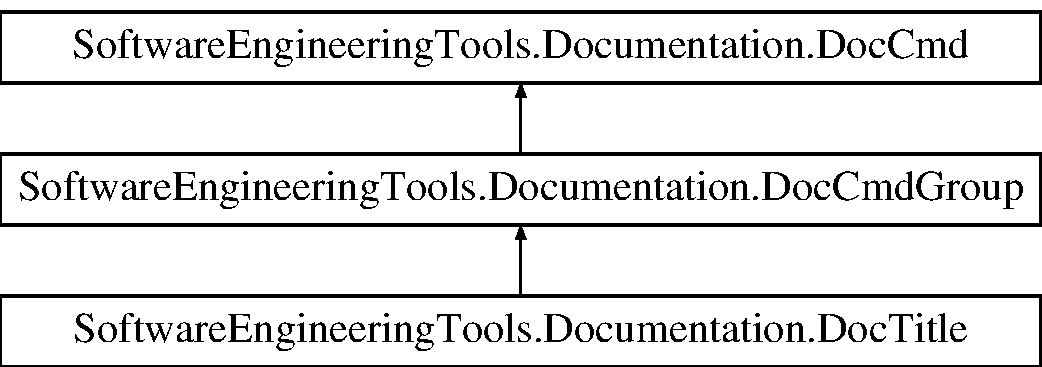
\includegraphics[height=3.000000cm]{class_software_engineering_tools_1_1_documentation_1_1_doc_title}
\end{center}
\end{figure}
\subsection*{Public Member Functions}
\begin{DoxyCompactItemize}
\item 
\hyperlink{class_software_engineering_tools_1_1_documentation_1_1_doc_title_a7b4a017d58809fcf76a89141f02f997a}{Doc\+Title} ()
\end{DoxyCompactItemize}
\subsection*{Additional Inherited Members}


\subsection{Detailed Description}


Definition at line 828 of file Doxygen.\+cs.



\subsection{Constructor \& Destructor Documentation}
\hypertarget{class_software_engineering_tools_1_1_documentation_1_1_doc_title_a7b4a017d58809fcf76a89141f02f997a}{\index{Software\+Engineering\+Tools\+::\+Documentation\+::\+Doc\+Title@{Software\+Engineering\+Tools\+::\+Documentation\+::\+Doc\+Title}!Doc\+Title@{Doc\+Title}}
\index{Doc\+Title@{Doc\+Title}!Software\+Engineering\+Tools\+::\+Documentation\+::\+Doc\+Title@{Software\+Engineering\+Tools\+::\+Documentation\+::\+Doc\+Title}}
\subsubsection[{Doc\+Title}]{\setlength{\rightskip}{0pt plus 5cm}Software\+Engineering\+Tools.\+Documentation.\+Doc\+Title.\+Doc\+Title (
\begin{DoxyParamCaption}
{}
\end{DoxyParamCaption}
)}}\label{class_software_engineering_tools_1_1_documentation_1_1_doc_title_a7b4a017d58809fcf76a89141f02f997a}


Definition at line 830 of file Doxygen.\+cs.



The documentation for this class was generated from the following file\+:\begin{DoxyCompactItemize}
\item 
Api\+Doc\+Lib/\hyperlink{_doxygen_8cs}{Doxygen.\+cs}\end{DoxyCompactItemize}

\hypertarget{class_software_engineering_tools_1_1_documentation_1_1_doc_toc_item}{\section{Software\+Engineering\+Tools.\+Documentation.\+Doc\+Toc\+Item Class Reference}
\label{class_software_engineering_tools_1_1_documentation_1_1_doc_toc_item}\index{Software\+Engineering\+Tools.\+Documentation.\+Doc\+Toc\+Item@{Software\+Engineering\+Tools.\+Documentation.\+Doc\+Toc\+Item}}
}
Inheritance diagram for Software\+Engineering\+Tools.\+Documentation.\+Doc\+Toc\+Item\+:\begin{figure}[H]
\begin{center}
\leavevmode
\includegraphics[height=3.000000cm]{class_software_engineering_tools_1_1_documentation_1_1_doc_toc_item}
\end{center}
\end{figure}
\subsection*{Public Member Functions}
\begin{DoxyCompactItemize}
\item 
\hyperlink{class_software_engineering_tools_1_1_documentation_1_1_doc_toc_item_abb7ea48ea2672db86dc03668ed5339fc}{Doc\+Toc\+Item} ()
\end{DoxyCompactItemize}
\subsection*{Properties}
\begin{DoxyCompactItemize}
\item 
string \hyperlink{class_software_engineering_tools_1_1_documentation_1_1_doc_toc_item_a141823f142882df4ad7cd66eefbf834e}{Id}\hspace{0.3cm}{\ttfamily  \mbox{[}get, set\mbox{]}}
\end{DoxyCompactItemize}


\subsection{Detailed Description}


Definition at line 941 of file Doxygen.\+cs.



\subsection{Constructor \& Destructor Documentation}
\hypertarget{class_software_engineering_tools_1_1_documentation_1_1_doc_toc_item_abb7ea48ea2672db86dc03668ed5339fc}{\index{Software\+Engineering\+Tools\+::\+Documentation\+::\+Doc\+Toc\+Item@{Software\+Engineering\+Tools\+::\+Documentation\+::\+Doc\+Toc\+Item}!Doc\+Toc\+Item@{Doc\+Toc\+Item}}
\index{Doc\+Toc\+Item@{Doc\+Toc\+Item}!Software\+Engineering\+Tools\+::\+Documentation\+::\+Doc\+Toc\+Item@{Software\+Engineering\+Tools\+::\+Documentation\+::\+Doc\+Toc\+Item}}
\subsubsection[{Doc\+Toc\+Item}]{\setlength{\rightskip}{0pt plus 5cm}Software\+Engineering\+Tools.\+Documentation.\+Doc\+Toc\+Item.\+Doc\+Toc\+Item (
\begin{DoxyParamCaption}
{}
\end{DoxyParamCaption}
)}}\label{class_software_engineering_tools_1_1_documentation_1_1_doc_toc_item_abb7ea48ea2672db86dc03668ed5339fc}


Definition at line 945 of file Doxygen.\+cs.



\subsection{Property Documentation}
\hypertarget{class_software_engineering_tools_1_1_documentation_1_1_doc_toc_item_a141823f142882df4ad7cd66eefbf834e}{\index{Software\+Engineering\+Tools\+::\+Documentation\+::\+Doc\+Toc\+Item@{Software\+Engineering\+Tools\+::\+Documentation\+::\+Doc\+Toc\+Item}!Id@{Id}}
\index{Id@{Id}!Software\+Engineering\+Tools\+::\+Documentation\+::\+Doc\+Toc\+Item@{Software\+Engineering\+Tools\+::\+Documentation\+::\+Doc\+Toc\+Item}}
\subsubsection[{Id}]{\setlength{\rightskip}{0pt plus 5cm}string Software\+Engineering\+Tools.\+Documentation.\+Doc\+Toc\+Item.\+Id\hspace{0.3cm}{\ttfamily [get]}, {\ttfamily [set]}}}\label{class_software_engineering_tools_1_1_documentation_1_1_doc_toc_item_a141823f142882df4ad7cd66eefbf834e}


Definition at line 943 of file Doxygen.\+cs.



The documentation for this class was generated from the following file\+:\begin{DoxyCompactItemize}
\item 
Api\+Doc\+Lib/\hyperlink{_doxygen_8cs}{Doxygen.\+cs}\end{DoxyCompactItemize}

\hypertarget{class_software_engineering_tools_1_1_documentation_1_1_doc_toc_list}{\section{Software\+Engineering\+Tools.\+Documentation.\+Doc\+Toc\+List Class Reference}
\label{class_software_engineering_tools_1_1_documentation_1_1_doc_toc_list}\index{Software\+Engineering\+Tools.\+Documentation.\+Doc\+Toc\+List@{Software\+Engineering\+Tools.\+Documentation.\+Doc\+Toc\+List}}
}
Inheritance diagram for Software\+Engineering\+Tools.\+Documentation.\+Doc\+Toc\+List\+:\begin{figure}[H]
\begin{center}
\leavevmode
\includegraphics[height=2.000000cm]{class_software_engineering_tools_1_1_documentation_1_1_doc_toc_list}
\end{center}
\end{figure}
\subsection*{Public Member Functions}
\begin{DoxyCompactItemize}
\item 
\hyperlink{class_software_engineering_tools_1_1_documentation_1_1_doc_toc_list_aa5b4b3df90602c001abc87ca73a805df}{Doc\+Toc\+List} ()
\end{DoxyCompactItemize}
\subsection*{Properties}
\begin{DoxyCompactItemize}
\item 
\hyperlink{namespace_software_engineering_tools_1_1_documentation_ae0bccf4f49a76db084c1c316e5954ec9a4ee29ca12c7d126654bd0e5275de6135}{List}$<$ \hyperlink{class_software_engineering_tools_1_1_documentation_1_1_doc_toc_item}{Doc\+Toc\+Item} $>$ \hyperlink{class_software_engineering_tools_1_1_documentation_1_1_doc_toc_list_a2651cd51e7a7cfd9aeb241ca842316dd}{Items}\hspace{0.3cm}{\ttfamily  \mbox{[}get, set\mbox{]}}
\end{DoxyCompactItemize}


\subsection{Detailed Description}


Definition at line 930 of file Doxygen.\+cs.



\subsection{Constructor \& Destructor Documentation}
\hypertarget{class_software_engineering_tools_1_1_documentation_1_1_doc_toc_list_aa5b4b3df90602c001abc87ca73a805df}{\index{Software\+Engineering\+Tools\+::\+Documentation\+::\+Doc\+Toc\+List@{Software\+Engineering\+Tools\+::\+Documentation\+::\+Doc\+Toc\+List}!Doc\+Toc\+List@{Doc\+Toc\+List}}
\index{Doc\+Toc\+List@{Doc\+Toc\+List}!Software\+Engineering\+Tools\+::\+Documentation\+::\+Doc\+Toc\+List@{Software\+Engineering\+Tools\+::\+Documentation\+::\+Doc\+Toc\+List}}
\subsubsection[{Doc\+Toc\+List}]{\setlength{\rightskip}{0pt plus 5cm}Software\+Engineering\+Tools.\+Documentation.\+Doc\+Toc\+List.\+Doc\+Toc\+List (
\begin{DoxyParamCaption}
{}
\end{DoxyParamCaption}
)}}\label{class_software_engineering_tools_1_1_documentation_1_1_doc_toc_list_aa5b4b3df90602c001abc87ca73a805df}


Definition at line 934 of file Doxygen.\+cs.



\subsection{Property Documentation}
\hypertarget{class_software_engineering_tools_1_1_documentation_1_1_doc_toc_list_a2651cd51e7a7cfd9aeb241ca842316dd}{\index{Software\+Engineering\+Tools\+::\+Documentation\+::\+Doc\+Toc\+List@{Software\+Engineering\+Tools\+::\+Documentation\+::\+Doc\+Toc\+List}!Items@{Items}}
\index{Items@{Items}!Software\+Engineering\+Tools\+::\+Documentation\+::\+Doc\+Toc\+List@{Software\+Engineering\+Tools\+::\+Documentation\+::\+Doc\+Toc\+List}}
\subsubsection[{Items}]{\setlength{\rightskip}{0pt plus 5cm}{\bf List}$<${\bf Doc\+Toc\+Item}$>$ Software\+Engineering\+Tools.\+Documentation.\+Doc\+Toc\+List.\+Items\hspace{0.3cm}{\ttfamily [get]}, {\ttfamily [set]}}}\label{class_software_engineering_tools_1_1_documentation_1_1_doc_toc_list_a2651cd51e7a7cfd9aeb241ca842316dd}


Definition at line 932 of file Doxygen.\+cs.



The documentation for this class was generated from the following file\+:\begin{DoxyCompactItemize}
\item 
Api\+Doc\+Lib/\hyperlink{_doxygen_8cs}{Doxygen.\+cs}\end{DoxyCompactItemize}

\hypertarget{class_software_engineering_tools_1_1_documentation_1_1_document_exception}{\section{Software\+Engineering\+Tools.\+Documentation.\+Document\+Exception Class Reference}
\label{class_software_engineering_tools_1_1_documentation_1_1_document_exception}\index{Software\+Engineering\+Tools.\+Documentation.\+Document\+Exception@{Software\+Engineering\+Tools.\+Documentation.\+Document\+Exception}}
}
Inheritance diagram for Software\+Engineering\+Tools.\+Documentation.\+Document\+Exception\+:\begin{figure}[H]
\begin{center}
\leavevmode
\includegraphics[height=2.000000cm]{class_software_engineering_tools_1_1_documentation_1_1_document_exception}
\end{center}
\end{figure}
\subsection*{Public Member Functions}
\begin{DoxyCompactItemize}
\item 
\hyperlink{class_software_engineering_tools_1_1_documentation_1_1_document_exception_a58122280f1857a8fbc9f0827ca096d6c}{Document\+Exception} ()
\item 
\hyperlink{class_software_engineering_tools_1_1_documentation_1_1_document_exception_af8026ba267419e75df82a02cd25648a8}{Document\+Exception} (string message)
\item 
\hyperlink{class_software_engineering_tools_1_1_documentation_1_1_document_exception_ac268dd481c1d85bf7abb917c0ca6b9e0}{Document\+Exception} (string message, \hyperlink{namespace_software_engineering_tools_1_1_documentation_aae490e51e07ef6e5540a2f2c04fccbb1ab0d4998a26f5b5742ad38c4af8817e32}{Exception} inner\+Exception)
\end{DoxyCompactItemize}


\subsection{Detailed Description}


Definition at line 8 of file Document\+Exception.\+cs.



\subsection{Constructor \& Destructor Documentation}
\hypertarget{class_software_engineering_tools_1_1_documentation_1_1_document_exception_a58122280f1857a8fbc9f0827ca096d6c}{\index{Software\+Engineering\+Tools\+::\+Documentation\+::\+Document\+Exception@{Software\+Engineering\+Tools\+::\+Documentation\+::\+Document\+Exception}!Document\+Exception@{Document\+Exception}}
\index{Document\+Exception@{Document\+Exception}!Software\+Engineering\+Tools\+::\+Documentation\+::\+Document\+Exception@{Software\+Engineering\+Tools\+::\+Documentation\+::\+Document\+Exception}}
\subsubsection[{Document\+Exception}]{\setlength{\rightskip}{0pt plus 5cm}Software\+Engineering\+Tools.\+Documentation.\+Document\+Exception.\+Document\+Exception (
\begin{DoxyParamCaption}
{}
\end{DoxyParamCaption}
)}}\label{class_software_engineering_tools_1_1_documentation_1_1_document_exception_a58122280f1857a8fbc9f0827ca096d6c}


Definition at line 10 of file Document\+Exception.\+cs.

\hypertarget{class_software_engineering_tools_1_1_documentation_1_1_document_exception_af8026ba267419e75df82a02cd25648a8}{\index{Software\+Engineering\+Tools\+::\+Documentation\+::\+Document\+Exception@{Software\+Engineering\+Tools\+::\+Documentation\+::\+Document\+Exception}!Document\+Exception@{Document\+Exception}}
\index{Document\+Exception@{Document\+Exception}!Software\+Engineering\+Tools\+::\+Documentation\+::\+Document\+Exception@{Software\+Engineering\+Tools\+::\+Documentation\+::\+Document\+Exception}}
\subsubsection[{Document\+Exception}]{\setlength{\rightskip}{0pt plus 5cm}Software\+Engineering\+Tools.\+Documentation.\+Document\+Exception.\+Document\+Exception (
\begin{DoxyParamCaption}
\item[{string}]{message}
\end{DoxyParamCaption}
)}}\label{class_software_engineering_tools_1_1_documentation_1_1_document_exception_af8026ba267419e75df82a02cd25648a8}


Definition at line 15 of file Document\+Exception.\+cs.

\hypertarget{class_software_engineering_tools_1_1_documentation_1_1_document_exception_ac268dd481c1d85bf7abb917c0ca6b9e0}{\index{Software\+Engineering\+Tools\+::\+Documentation\+::\+Document\+Exception@{Software\+Engineering\+Tools\+::\+Documentation\+::\+Document\+Exception}!Document\+Exception@{Document\+Exception}}
\index{Document\+Exception@{Document\+Exception}!Software\+Engineering\+Tools\+::\+Documentation\+::\+Document\+Exception@{Software\+Engineering\+Tools\+::\+Documentation\+::\+Document\+Exception}}
\subsubsection[{Document\+Exception}]{\setlength{\rightskip}{0pt plus 5cm}Software\+Engineering\+Tools.\+Documentation.\+Document\+Exception.\+Document\+Exception (
\begin{DoxyParamCaption}
\item[{string}]{message, }
\item[{{\bf Exception}}]{inner\+Exception}
\end{DoxyParamCaption}
)}}\label{class_software_engineering_tools_1_1_documentation_1_1_document_exception_ac268dd481c1d85bf7abb917c0ca6b9e0}


Definition at line 20 of file Document\+Exception.\+cs.



The documentation for this class was generated from the following file\+:\begin{DoxyCompactItemize}
\item 
Document\+Generator\+Lib/\hyperlink{_document_exception_8cs}{Document\+Exception.\+cs}\end{DoxyCompactItemize}

\hypertarget{class_software_engineering_tools_1_1_documentation_1_1_document_generator}{\section{Software\+Engineering\+Tools.\+Documentation.\+Document\+Generator Class Reference}
\label{class_software_engineering_tools_1_1_documentation_1_1_document_generator}\index{Software\+Engineering\+Tools.\+Documentation.\+Document\+Generator@{Software\+Engineering\+Tools.\+Documentation.\+Document\+Generator}}
}
Inheritance diagram for Software\+Engineering\+Tools.\+Documentation.\+Document\+Generator\+:\begin{figure}[H]
\begin{center}
\leavevmode
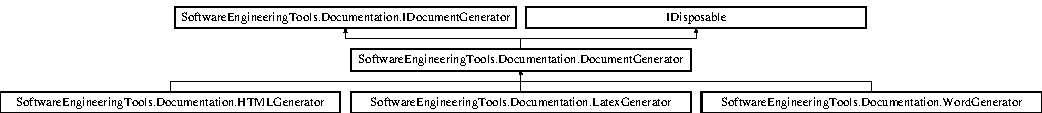
\includegraphics[height=1.493333cm]{class_software_engineering_tools_1_1_documentation_1_1_document_generator}
\end{center}
\end{figure}
\subsection*{Public Member Functions}
\begin{DoxyCompactItemize}
\item 
abstract void \hyperlink{class_software_engineering_tools_1_1_documentation_1_1_document_generator_a9fe08809c64a81d6a915169cd655cc3f}{Dispose} ()
\item 
abstract void \hyperlink{class_software_engineering_tools_1_1_documentation_1_1_document_generator_aa6b7b1a10a275fa3833f79c21ad932f8}{Begin\+Section\+Title} (\hyperlink{namespace_software_engineering_tools_1_1_documentation_a4a8017aa254d1d05b03db5132b7dd3a7afa7153f7ed1cb6c0fcf2ffb2fac21748}{int} level, string title, string label)
\item 
abstract void \hyperlink{class_software_engineering_tools_1_1_documentation_1_1_document_generator_af39f74148f77d9e036a9a3b284c4d569}{Set\+Content} (bool enabled, \hyperlink{namespace_software_engineering_tools_1_1_documentation_a4a8017aa254d1d05b03db5132b7dd3a7afa7153f7ed1cb6c0fcf2ffb2fac21748}{int} depth)
\item 
abstract void \hyperlink{class_software_engineering_tools_1_1_documentation_1_1_document_generator_a649acf880cf5cdbdf3fe71924de0954e}{End\+Section\+Title} ()
\item 
abstract void \hyperlink{class_software_engineering_tools_1_1_documentation_1_1_document_generator_a589f93438eceb47c5fae148ec40418a6}{New\+Paragraph} ()
\item 
abstract void \hyperlink{class_software_engineering_tools_1_1_documentation_1_1_document_generator_a17021c5059b0dee77f60d085567d6265}{Print\+Text} (string text, bool insert\+Space=true)
\item 
abstract void \hyperlink{class_software_engineering_tools_1_1_documentation_1_1_document_generator_a9806a5f0d5c0fea55cc7247ca6ea1d70}{Print\+Verbatim\+Text} (string text)
\item 
abstract void \hyperlink{class_software_engineering_tools_1_1_documentation_1_1_document_generator_a9398de502d89f600ac1f8ec72e6f1f48}{Begin\+Markup} (\hyperlink{namespace_software_engineering_tools_1_1_documentation_a4eed17ca0ed06a8b62b953b063f857d9}{Document\+Markup\+Kind} markup\+Kind)
\item 
abstract void \hyperlink{class_software_engineering_tools_1_1_documentation_1_1_document_generator_a11ff9fa315e40775e63fd2b4dc184596}{End\+Markup} (\hyperlink{namespace_software_engineering_tools_1_1_documentation_a4eed17ca0ed06a8b62b953b063f857d9}{Document\+Markup\+Kind} markup\+Kind)
\item 
abstract void \hyperlink{class_software_engineering_tools_1_1_documentation_1_1_document_generator_a6e0fb6c2edbb674ec4f0048ac1984871}{New\+Label} (string id)
\item 
abstract void \hyperlink{class_software_engineering_tools_1_1_documentation_1_1_document_generator_aacc6cff53b0298213c5bfbbae5cf39ec}{Begin\+Reference} (string id, bool url)
\item 
abstract void \hyperlink{class_software_engineering_tools_1_1_documentation_1_1_document_generator_a6bf9ae60215596599442591d3f8e2636}{End\+Reference} ()
\item 
abstract void \hyperlink{class_software_engineering_tools_1_1_documentation_1_1_document_generator_ac293a5f636676bbf7f4183e9aa4439e5}{Begin\+List} ()
\item 
abstract void \hyperlink{class_software_engineering_tools_1_1_documentation_1_1_document_generator_a06d3076fc6cb5f27e0573fdbc79aa879}{End\+List} ()
\item 
abstract void \hyperlink{class_software_engineering_tools_1_1_documentation_1_1_document_generator_aebd2eac27c0ff8a1dcb9a9e4914a54b6}{Begin\+List\+Item} (\hyperlink{namespace_software_engineering_tools_1_1_documentation_a4a8017aa254d1d05b03db5132b7dd3a7afa7153f7ed1cb6c0fcf2ffb2fac21748}{int} index, string title)
\item 
abstract void \hyperlink{class_software_engineering_tools_1_1_documentation_1_1_document_generator_a6cf51dcd959fe8b91f5278dc508cd704}{End\+List\+Item} (\hyperlink{namespace_software_engineering_tools_1_1_documentation_a4a8017aa254d1d05b03db5132b7dd3a7afa7153f7ed1cb6c0fcf2ffb2fac21748}{int} index)
\item 
abstract void \hyperlink{class_software_engineering_tools_1_1_documentation_1_1_document_generator_a0b1b0b9fa405181afcca7297b0c429d7}{Begin\+Table} (\hyperlink{namespace_software_engineering_tools_1_1_documentation_a4a8017aa254d1d05b03db5132b7dd3a7afa7153f7ed1cb6c0fcf2ffb2fac21748}{int} row\+Count, \hyperlink{namespace_software_engineering_tools_1_1_documentation_a4a8017aa254d1d05b03db5132b7dd3a7afa7153f7ed1cb6c0fcf2ffb2fac21748}{int} col\+Count)
\item 
abstract void \hyperlink{class_software_engineering_tools_1_1_documentation_1_1_document_generator_a11ff1e9792b49b59731026e57040b3d4}{Begin\+Table\+Row} (\hyperlink{namespace_software_engineering_tools_1_1_documentation_a4a8017aa254d1d05b03db5132b7dd3a7afa7153f7ed1cb6c0fcf2ffb2fac21748}{int} row\+Index)
\item 
abstract void \hyperlink{class_software_engineering_tools_1_1_documentation_1_1_document_generator_a0c815504fc6e9d7e2c49f114fdd93a88}{End\+Table\+Row} (\hyperlink{namespace_software_engineering_tools_1_1_documentation_a4a8017aa254d1d05b03db5132b7dd3a7afa7153f7ed1cb6c0fcf2ffb2fac21748}{int} index)
\item 
abstract void \hyperlink{class_software_engineering_tools_1_1_documentation_1_1_document_generator_a142486e159cf18396bad17686c4ece3b}{Begin\+Table\+Cell} (\hyperlink{namespace_software_engineering_tools_1_1_documentation_a4a8017aa254d1d05b03db5132b7dd3a7afa7153f7ed1cb6c0fcf2ffb2fac21748}{int} row\+Index, \hyperlink{namespace_software_engineering_tools_1_1_documentation_a4a8017aa254d1d05b03db5132b7dd3a7afa7153f7ed1cb6c0fcf2ffb2fac21748}{int} col\+Index, bool head)
\item 
abstract void \hyperlink{class_software_engineering_tools_1_1_documentation_1_1_document_generator_ad7358d1047a392ce8d23e01d6c541e72}{End\+Table\+Cell} (\hyperlink{namespace_software_engineering_tools_1_1_documentation_a4a8017aa254d1d05b03db5132b7dd3a7afa7153f7ed1cb6c0fcf2ffb2fac21748}{int} row\+Index, \hyperlink{namespace_software_engineering_tools_1_1_documentation_a4a8017aa254d1d05b03db5132b7dd3a7afa7153f7ed1cb6c0fcf2ffb2fac21748}{int} col\+Index, bool head)
\item 
abstract void \hyperlink{class_software_engineering_tools_1_1_documentation_1_1_document_generator_a6244abdf686183395fb44339111a7363}{End\+Table} ()
\end{DoxyCompactItemize}
\subsection*{Protected Member Functions}
\begin{DoxyCompactItemize}
\item 
abstract void \hyperlink{class_software_engineering_tools_1_1_documentation_1_1_document_generator_a6dcea40e796970bba1229a2e513fdb56}{Begin\+Document} ()
\item 
abstract void \hyperlink{class_software_engineering_tools_1_1_documentation_1_1_document_generator_ae367934e4153adfd260dec902d0e69d5}{End\+Document} ()
\end{DoxyCompactItemize}


\subsection{Detailed Description}


Definition at line 46 of file Document\+Generator.\+cs.



\subsection{Member Function Documentation}
\hypertarget{class_software_engineering_tools_1_1_documentation_1_1_document_generator_a6dcea40e796970bba1229a2e513fdb56}{\index{Software\+Engineering\+Tools\+::\+Documentation\+::\+Document\+Generator@{Software\+Engineering\+Tools\+::\+Documentation\+::\+Document\+Generator}!Begin\+Document@{Begin\+Document}}
\index{Begin\+Document@{Begin\+Document}!Software\+Engineering\+Tools\+::\+Documentation\+::\+Document\+Generator@{Software\+Engineering\+Tools\+::\+Documentation\+::\+Document\+Generator}}
\subsubsection[{Begin\+Document}]{\setlength{\rightskip}{0pt plus 5cm}abstract void Software\+Engineering\+Tools.\+Documentation.\+Document\+Generator.\+Begin\+Document (
\begin{DoxyParamCaption}
{}
\end{DoxyParamCaption}
)\hspace{0.3cm}{\ttfamily [protected]}, {\ttfamily [pure virtual]}}}\label{class_software_engineering_tools_1_1_documentation_1_1_document_generator_a6dcea40e796970bba1229a2e513fdb56}


Implemented in \hyperlink{class_software_engineering_tools_1_1_documentation_1_1_word_generator_a8bde307f2f0e1951ef630820826d87d0}{Software\+Engineering\+Tools.\+Documentation.\+Word\+Generator}, \hyperlink{class_software_engineering_tools_1_1_documentation_1_1_h_t_m_l_generator_ab9828a528be4027dc37c6f674a40e007}{Software\+Engineering\+Tools.\+Documentation.\+H\+T\+M\+L\+Generator}, and \hyperlink{class_software_engineering_tools_1_1_documentation_1_1_latex_generator_a415cd0402059b26675d15c4679013635}{Software\+Engineering\+Tools.\+Documentation.\+Latex\+Generator}.

\hypertarget{class_software_engineering_tools_1_1_documentation_1_1_document_generator_ac293a5f636676bbf7f4183e9aa4439e5}{\index{Software\+Engineering\+Tools\+::\+Documentation\+::\+Document\+Generator@{Software\+Engineering\+Tools\+::\+Documentation\+::\+Document\+Generator}!Begin\+List@{Begin\+List}}
\index{Begin\+List@{Begin\+List}!Software\+Engineering\+Tools\+::\+Documentation\+::\+Document\+Generator@{Software\+Engineering\+Tools\+::\+Documentation\+::\+Document\+Generator}}
\subsubsection[{Begin\+List}]{\setlength{\rightskip}{0pt plus 5cm}abstract void Software\+Engineering\+Tools.\+Documentation.\+Document\+Generator.\+Begin\+List (
\begin{DoxyParamCaption}
{}
\end{DoxyParamCaption}
)\hspace{0.3cm}{\ttfamily [pure virtual]}}}\label{class_software_engineering_tools_1_1_documentation_1_1_document_generator_ac293a5f636676bbf7f4183e9aa4439e5}


Implements \hyperlink{interface_software_engineering_tools_1_1_documentation_1_1_i_document_generator_a8bb16673fa645991c4ff1c27f3fc78c5}{Software\+Engineering\+Tools.\+Documentation.\+I\+Document\+Generator}.



Implemented in \hyperlink{class_software_engineering_tools_1_1_documentation_1_1_word_generator_a8e6c89f64b72dc406aab016d39ee3c60}{Software\+Engineering\+Tools.\+Documentation.\+Word\+Generator}, \hyperlink{class_software_engineering_tools_1_1_documentation_1_1_h_t_m_l_generator_a18d52185703fa6da3727b26297917383}{Software\+Engineering\+Tools.\+Documentation.\+H\+T\+M\+L\+Generator}, and \hyperlink{class_software_engineering_tools_1_1_documentation_1_1_latex_generator_a7341918f8ef12c497964a3da86681b4a}{Software\+Engineering\+Tools.\+Documentation.\+Latex\+Generator}.

\hypertarget{class_software_engineering_tools_1_1_documentation_1_1_document_generator_aebd2eac27c0ff8a1dcb9a9e4914a54b6}{\index{Software\+Engineering\+Tools\+::\+Documentation\+::\+Document\+Generator@{Software\+Engineering\+Tools\+::\+Documentation\+::\+Document\+Generator}!Begin\+List\+Item@{Begin\+List\+Item}}
\index{Begin\+List\+Item@{Begin\+List\+Item}!Software\+Engineering\+Tools\+::\+Documentation\+::\+Document\+Generator@{Software\+Engineering\+Tools\+::\+Documentation\+::\+Document\+Generator}}
\subsubsection[{Begin\+List\+Item}]{\setlength{\rightskip}{0pt plus 5cm}abstract void Software\+Engineering\+Tools.\+Documentation.\+Document\+Generator.\+Begin\+List\+Item (
\begin{DoxyParamCaption}
\item[{{\bf int}}]{index, }
\item[{string}]{title}
\end{DoxyParamCaption}
)\hspace{0.3cm}{\ttfamily [pure virtual]}}}\label{class_software_engineering_tools_1_1_documentation_1_1_document_generator_aebd2eac27c0ff8a1dcb9a9e4914a54b6}


Implements \hyperlink{interface_software_engineering_tools_1_1_documentation_1_1_i_document_generator_aa6c2854f4670d91a3f16ff52b01c1d44}{Software\+Engineering\+Tools.\+Documentation.\+I\+Document\+Generator}.



Implemented in \hyperlink{class_software_engineering_tools_1_1_documentation_1_1_word_generator_a21cf3f4b0aabac4e3a64b0da78cd0212}{Software\+Engineering\+Tools.\+Documentation.\+Word\+Generator}, \hyperlink{class_software_engineering_tools_1_1_documentation_1_1_h_t_m_l_generator_a4da5442652b4dcd06bd011f43cd0c6ea}{Software\+Engineering\+Tools.\+Documentation.\+H\+T\+M\+L\+Generator}, and \hyperlink{class_software_engineering_tools_1_1_documentation_1_1_latex_generator_a5c8335a734a3a1df797b23fbb660cfdf}{Software\+Engineering\+Tools.\+Documentation.\+Latex\+Generator}.

\hypertarget{class_software_engineering_tools_1_1_documentation_1_1_document_generator_a9398de502d89f600ac1f8ec72e6f1f48}{\index{Software\+Engineering\+Tools\+::\+Documentation\+::\+Document\+Generator@{Software\+Engineering\+Tools\+::\+Documentation\+::\+Document\+Generator}!Begin\+Markup@{Begin\+Markup}}
\index{Begin\+Markup@{Begin\+Markup}!Software\+Engineering\+Tools\+::\+Documentation\+::\+Document\+Generator@{Software\+Engineering\+Tools\+::\+Documentation\+::\+Document\+Generator}}
\subsubsection[{Begin\+Markup}]{\setlength{\rightskip}{0pt plus 5cm}abstract void Software\+Engineering\+Tools.\+Documentation.\+Document\+Generator.\+Begin\+Markup (
\begin{DoxyParamCaption}
\item[{{\bf Document\+Markup\+Kind}}]{markup\+Kind}
\end{DoxyParamCaption}
)\hspace{0.3cm}{\ttfamily [pure virtual]}}}\label{class_software_engineering_tools_1_1_documentation_1_1_document_generator_a9398de502d89f600ac1f8ec72e6f1f48}


Implements \hyperlink{interface_software_engineering_tools_1_1_documentation_1_1_i_document_generator_a3cc12daff5435cee9b1ab979cf16fa02}{Software\+Engineering\+Tools.\+Documentation.\+I\+Document\+Generator}.



Implemented in \hyperlink{class_software_engineering_tools_1_1_documentation_1_1_word_generator_a7606e1f460a2b58245d6dd1418058a11}{Software\+Engineering\+Tools.\+Documentation.\+Word\+Generator}, \hyperlink{class_software_engineering_tools_1_1_documentation_1_1_h_t_m_l_generator_abf50ab24cd3a1112940a09542c1cb787}{Software\+Engineering\+Tools.\+Documentation.\+H\+T\+M\+L\+Generator}, and \hyperlink{class_software_engineering_tools_1_1_documentation_1_1_latex_generator_ad6732108c1739d704defce5722e112ad}{Software\+Engineering\+Tools.\+Documentation.\+Latex\+Generator}.

\hypertarget{class_software_engineering_tools_1_1_documentation_1_1_document_generator_aacc6cff53b0298213c5bfbbae5cf39ec}{\index{Software\+Engineering\+Tools\+::\+Documentation\+::\+Document\+Generator@{Software\+Engineering\+Tools\+::\+Documentation\+::\+Document\+Generator}!Begin\+Reference@{Begin\+Reference}}
\index{Begin\+Reference@{Begin\+Reference}!Software\+Engineering\+Tools\+::\+Documentation\+::\+Document\+Generator@{Software\+Engineering\+Tools\+::\+Documentation\+::\+Document\+Generator}}
\subsubsection[{Begin\+Reference}]{\setlength{\rightskip}{0pt plus 5cm}abstract void Software\+Engineering\+Tools.\+Documentation.\+Document\+Generator.\+Begin\+Reference (
\begin{DoxyParamCaption}
\item[{string}]{id, }
\item[{bool}]{url}
\end{DoxyParamCaption}
)\hspace{0.3cm}{\ttfamily [pure virtual]}}}\label{class_software_engineering_tools_1_1_documentation_1_1_document_generator_aacc6cff53b0298213c5bfbbae5cf39ec}


Implements \hyperlink{interface_software_engineering_tools_1_1_documentation_1_1_i_document_generator_a7fa263ab2571b238abf44eca3cf1f0bc}{Software\+Engineering\+Tools.\+Documentation.\+I\+Document\+Generator}.



Implemented in \hyperlink{class_software_engineering_tools_1_1_documentation_1_1_word_generator_acdb54490629705960c7544904a96f8b9}{Software\+Engineering\+Tools.\+Documentation.\+Word\+Generator}, \hyperlink{class_software_engineering_tools_1_1_documentation_1_1_h_t_m_l_generator_ae6cd34a01a45c94485bc4d50d7e065b7}{Software\+Engineering\+Tools.\+Documentation.\+H\+T\+M\+L\+Generator}, and \hyperlink{class_software_engineering_tools_1_1_documentation_1_1_latex_generator_aa48cc264ca9a70e82b25c25fd8cbd460}{Software\+Engineering\+Tools.\+Documentation.\+Latex\+Generator}.

\hypertarget{class_software_engineering_tools_1_1_documentation_1_1_document_generator_aa6b7b1a10a275fa3833f79c21ad932f8}{\index{Software\+Engineering\+Tools\+::\+Documentation\+::\+Document\+Generator@{Software\+Engineering\+Tools\+::\+Documentation\+::\+Document\+Generator}!Begin\+Section\+Title@{Begin\+Section\+Title}}
\index{Begin\+Section\+Title@{Begin\+Section\+Title}!Software\+Engineering\+Tools\+::\+Documentation\+::\+Document\+Generator@{Software\+Engineering\+Tools\+::\+Documentation\+::\+Document\+Generator}}
\subsubsection[{Begin\+Section\+Title}]{\setlength{\rightskip}{0pt plus 5cm}abstract void Software\+Engineering\+Tools.\+Documentation.\+Document\+Generator.\+Begin\+Section\+Title (
\begin{DoxyParamCaption}
\item[{{\bf int}}]{level, }
\item[{string}]{title, }
\item[{string}]{label}
\end{DoxyParamCaption}
)\hspace{0.3cm}{\ttfamily [pure virtual]}}}\label{class_software_engineering_tools_1_1_documentation_1_1_document_generator_aa6b7b1a10a275fa3833f79c21ad932f8}


Implements \hyperlink{interface_software_engineering_tools_1_1_documentation_1_1_i_document_generator_a8f4c05966722692fccdd777204393380}{Software\+Engineering\+Tools.\+Documentation.\+I\+Document\+Generator}.



Implemented in \hyperlink{class_software_engineering_tools_1_1_documentation_1_1_word_generator_accc00e23ef4d7fa36359715ce4bd3845}{Software\+Engineering\+Tools.\+Documentation.\+Word\+Generator}, \hyperlink{class_software_engineering_tools_1_1_documentation_1_1_h_t_m_l_generator_a22166b2d3e73aba20bdc9a5d49c0a1e0}{Software\+Engineering\+Tools.\+Documentation.\+H\+T\+M\+L\+Generator}, and \hyperlink{class_software_engineering_tools_1_1_documentation_1_1_latex_generator_a0987b0d6682e4edabf9df277a382eecb}{Software\+Engineering\+Tools.\+Documentation.\+Latex\+Generator}.

\hypertarget{class_software_engineering_tools_1_1_documentation_1_1_document_generator_a0b1b0b9fa405181afcca7297b0c429d7}{\index{Software\+Engineering\+Tools\+::\+Documentation\+::\+Document\+Generator@{Software\+Engineering\+Tools\+::\+Documentation\+::\+Document\+Generator}!Begin\+Table@{Begin\+Table}}
\index{Begin\+Table@{Begin\+Table}!Software\+Engineering\+Tools\+::\+Documentation\+::\+Document\+Generator@{Software\+Engineering\+Tools\+::\+Documentation\+::\+Document\+Generator}}
\subsubsection[{Begin\+Table}]{\setlength{\rightskip}{0pt plus 5cm}abstract void Software\+Engineering\+Tools.\+Documentation.\+Document\+Generator.\+Begin\+Table (
\begin{DoxyParamCaption}
\item[{{\bf int}}]{row\+Count, }
\item[{{\bf int}}]{col\+Count}
\end{DoxyParamCaption}
)\hspace{0.3cm}{\ttfamily [pure virtual]}}}\label{class_software_engineering_tools_1_1_documentation_1_1_document_generator_a0b1b0b9fa405181afcca7297b0c429d7}


Implements \hyperlink{interface_software_engineering_tools_1_1_documentation_1_1_i_document_generator_a5d8fb01ae06f90081dd3a963bcd9f651}{Software\+Engineering\+Tools.\+Documentation.\+I\+Document\+Generator}.



Implemented in \hyperlink{class_software_engineering_tools_1_1_documentation_1_1_word_generator_ad25649a8518696de278f7e7c9e36b86f}{Software\+Engineering\+Tools.\+Documentation.\+Word\+Generator}, \hyperlink{class_software_engineering_tools_1_1_documentation_1_1_h_t_m_l_generator_a67e1d82b87791489e744011aeef987df}{Software\+Engineering\+Tools.\+Documentation.\+H\+T\+M\+L\+Generator}, and \hyperlink{class_software_engineering_tools_1_1_documentation_1_1_latex_generator_a22a8ae8070617740885509fab8fbb1f1}{Software\+Engineering\+Tools.\+Documentation.\+Latex\+Generator}.

\hypertarget{class_software_engineering_tools_1_1_documentation_1_1_document_generator_a142486e159cf18396bad17686c4ece3b}{\index{Software\+Engineering\+Tools\+::\+Documentation\+::\+Document\+Generator@{Software\+Engineering\+Tools\+::\+Documentation\+::\+Document\+Generator}!Begin\+Table\+Cell@{Begin\+Table\+Cell}}
\index{Begin\+Table\+Cell@{Begin\+Table\+Cell}!Software\+Engineering\+Tools\+::\+Documentation\+::\+Document\+Generator@{Software\+Engineering\+Tools\+::\+Documentation\+::\+Document\+Generator}}
\subsubsection[{Begin\+Table\+Cell}]{\setlength{\rightskip}{0pt plus 5cm}abstract void Software\+Engineering\+Tools.\+Documentation.\+Document\+Generator.\+Begin\+Table\+Cell (
\begin{DoxyParamCaption}
\item[{{\bf int}}]{row\+Index, }
\item[{{\bf int}}]{col\+Index, }
\item[{bool}]{head}
\end{DoxyParamCaption}
)\hspace{0.3cm}{\ttfamily [pure virtual]}}}\label{class_software_engineering_tools_1_1_documentation_1_1_document_generator_a142486e159cf18396bad17686c4ece3b}


Implements \hyperlink{interface_software_engineering_tools_1_1_documentation_1_1_i_document_generator_ad66435c1af84d56700e94b5dbc3b9b61}{Software\+Engineering\+Tools.\+Documentation.\+I\+Document\+Generator}.



Implemented in \hyperlink{class_software_engineering_tools_1_1_documentation_1_1_word_generator_a6cca87392b3e19aa9517edf9d9fec1bc}{Software\+Engineering\+Tools.\+Documentation.\+Word\+Generator}, \hyperlink{class_software_engineering_tools_1_1_documentation_1_1_h_t_m_l_generator_a6450dee7b6db74a546d63e6dddeb319e}{Software\+Engineering\+Tools.\+Documentation.\+H\+T\+M\+L\+Generator}, and \hyperlink{class_software_engineering_tools_1_1_documentation_1_1_latex_generator_a332122bd834cdb6857fab0d76032ffe8}{Software\+Engineering\+Tools.\+Documentation.\+Latex\+Generator}.

\hypertarget{class_software_engineering_tools_1_1_documentation_1_1_document_generator_a11ff1e9792b49b59731026e57040b3d4}{\index{Software\+Engineering\+Tools\+::\+Documentation\+::\+Document\+Generator@{Software\+Engineering\+Tools\+::\+Documentation\+::\+Document\+Generator}!Begin\+Table\+Row@{Begin\+Table\+Row}}
\index{Begin\+Table\+Row@{Begin\+Table\+Row}!Software\+Engineering\+Tools\+::\+Documentation\+::\+Document\+Generator@{Software\+Engineering\+Tools\+::\+Documentation\+::\+Document\+Generator}}
\subsubsection[{Begin\+Table\+Row}]{\setlength{\rightskip}{0pt plus 5cm}abstract void Software\+Engineering\+Tools.\+Documentation.\+Document\+Generator.\+Begin\+Table\+Row (
\begin{DoxyParamCaption}
\item[{{\bf int}}]{row\+Index}
\end{DoxyParamCaption}
)\hspace{0.3cm}{\ttfamily [pure virtual]}}}\label{class_software_engineering_tools_1_1_documentation_1_1_document_generator_a11ff1e9792b49b59731026e57040b3d4}


Implements \hyperlink{interface_software_engineering_tools_1_1_documentation_1_1_i_document_generator_a02fae45bd4fcfa6487bb6bafe640a6a3}{Software\+Engineering\+Tools.\+Documentation.\+I\+Document\+Generator}.



Implemented in \hyperlink{class_software_engineering_tools_1_1_documentation_1_1_word_generator_a4d8c494b4539d97470ea2117a4534439}{Software\+Engineering\+Tools.\+Documentation.\+Word\+Generator}, \hyperlink{class_software_engineering_tools_1_1_documentation_1_1_h_t_m_l_generator_a1432777280c430247384c5e489dbfd61}{Software\+Engineering\+Tools.\+Documentation.\+H\+T\+M\+L\+Generator}, and \hyperlink{class_software_engineering_tools_1_1_documentation_1_1_latex_generator_a285da4d48fe002d10b25a5355317c89d}{Software\+Engineering\+Tools.\+Documentation.\+Latex\+Generator}.

\hypertarget{class_software_engineering_tools_1_1_documentation_1_1_document_generator_a9fe08809c64a81d6a915169cd655cc3f}{\index{Software\+Engineering\+Tools\+::\+Documentation\+::\+Document\+Generator@{Software\+Engineering\+Tools\+::\+Documentation\+::\+Document\+Generator}!Dispose@{Dispose}}
\index{Dispose@{Dispose}!Software\+Engineering\+Tools\+::\+Documentation\+::\+Document\+Generator@{Software\+Engineering\+Tools\+::\+Documentation\+::\+Document\+Generator}}
\subsubsection[{Dispose}]{\setlength{\rightskip}{0pt plus 5cm}abstract void Software\+Engineering\+Tools.\+Documentation.\+Document\+Generator.\+Dispose (
\begin{DoxyParamCaption}
{}
\end{DoxyParamCaption}
)\hspace{0.3cm}{\ttfamily [pure virtual]}}}\label{class_software_engineering_tools_1_1_documentation_1_1_document_generator_a9fe08809c64a81d6a915169cd655cc3f}


Implemented in \hyperlink{class_software_engineering_tools_1_1_documentation_1_1_word_generator_adf9f0b03760f695ece98b7c529de9e08}{Software\+Engineering\+Tools.\+Documentation.\+Word\+Generator}, \hyperlink{class_software_engineering_tools_1_1_documentation_1_1_h_t_m_l_generator_adfcd6c7e94631406dc3ce075c62317ef}{Software\+Engineering\+Tools.\+Documentation.\+H\+T\+M\+L\+Generator}, and \hyperlink{class_software_engineering_tools_1_1_documentation_1_1_latex_generator_a87139c6552aa29fbfdc20e07175ca9b5}{Software\+Engineering\+Tools.\+Documentation.\+Latex\+Generator}.

\hypertarget{class_software_engineering_tools_1_1_documentation_1_1_document_generator_ae367934e4153adfd260dec902d0e69d5}{\index{Software\+Engineering\+Tools\+::\+Documentation\+::\+Document\+Generator@{Software\+Engineering\+Tools\+::\+Documentation\+::\+Document\+Generator}!End\+Document@{End\+Document}}
\index{End\+Document@{End\+Document}!Software\+Engineering\+Tools\+::\+Documentation\+::\+Document\+Generator@{Software\+Engineering\+Tools\+::\+Documentation\+::\+Document\+Generator}}
\subsubsection[{End\+Document}]{\setlength{\rightskip}{0pt plus 5cm}abstract void Software\+Engineering\+Tools.\+Documentation.\+Document\+Generator.\+End\+Document (
\begin{DoxyParamCaption}
{}
\end{DoxyParamCaption}
)\hspace{0.3cm}{\ttfamily [protected]}, {\ttfamily [pure virtual]}}}\label{class_software_engineering_tools_1_1_documentation_1_1_document_generator_ae367934e4153adfd260dec902d0e69d5}


Implemented in \hyperlink{class_software_engineering_tools_1_1_documentation_1_1_word_generator_a0aadbc1dd71ab337f09e4e939915666e}{Software\+Engineering\+Tools.\+Documentation.\+Word\+Generator}, \hyperlink{class_software_engineering_tools_1_1_documentation_1_1_h_t_m_l_generator_af1190908a9867c982c993ab8a596435b}{Software\+Engineering\+Tools.\+Documentation.\+H\+T\+M\+L\+Generator}, and \hyperlink{class_software_engineering_tools_1_1_documentation_1_1_latex_generator_a24103014a84ca959b9df44d9c298af48}{Software\+Engineering\+Tools.\+Documentation.\+Latex\+Generator}.

\hypertarget{class_software_engineering_tools_1_1_documentation_1_1_document_generator_a06d3076fc6cb5f27e0573fdbc79aa879}{\index{Software\+Engineering\+Tools\+::\+Documentation\+::\+Document\+Generator@{Software\+Engineering\+Tools\+::\+Documentation\+::\+Document\+Generator}!End\+List@{End\+List}}
\index{End\+List@{End\+List}!Software\+Engineering\+Tools\+::\+Documentation\+::\+Document\+Generator@{Software\+Engineering\+Tools\+::\+Documentation\+::\+Document\+Generator}}
\subsubsection[{End\+List}]{\setlength{\rightskip}{0pt plus 5cm}abstract void Software\+Engineering\+Tools.\+Documentation.\+Document\+Generator.\+End\+List (
\begin{DoxyParamCaption}
{}
\end{DoxyParamCaption}
)\hspace{0.3cm}{\ttfamily [pure virtual]}}}\label{class_software_engineering_tools_1_1_documentation_1_1_document_generator_a06d3076fc6cb5f27e0573fdbc79aa879}


Implements \hyperlink{interface_software_engineering_tools_1_1_documentation_1_1_i_document_generator_ab1245da1f965e0970ee6e9ed8f896621}{Software\+Engineering\+Tools.\+Documentation.\+I\+Document\+Generator}.



Implemented in \hyperlink{class_software_engineering_tools_1_1_documentation_1_1_word_generator_a254b01c1abbc805bce33d0827ca12988}{Software\+Engineering\+Tools.\+Documentation.\+Word\+Generator}, \hyperlink{class_software_engineering_tools_1_1_documentation_1_1_h_t_m_l_generator_a65fa0e91f8157b674d922dd5800d14d0}{Software\+Engineering\+Tools.\+Documentation.\+H\+T\+M\+L\+Generator}, and \hyperlink{class_software_engineering_tools_1_1_documentation_1_1_latex_generator_a9e77a36261f8f09aa84cf7d15474bf6a}{Software\+Engineering\+Tools.\+Documentation.\+Latex\+Generator}.

\hypertarget{class_software_engineering_tools_1_1_documentation_1_1_document_generator_a6cf51dcd959fe8b91f5278dc508cd704}{\index{Software\+Engineering\+Tools\+::\+Documentation\+::\+Document\+Generator@{Software\+Engineering\+Tools\+::\+Documentation\+::\+Document\+Generator}!End\+List\+Item@{End\+List\+Item}}
\index{End\+List\+Item@{End\+List\+Item}!Software\+Engineering\+Tools\+::\+Documentation\+::\+Document\+Generator@{Software\+Engineering\+Tools\+::\+Documentation\+::\+Document\+Generator}}
\subsubsection[{End\+List\+Item}]{\setlength{\rightskip}{0pt plus 5cm}abstract void Software\+Engineering\+Tools.\+Documentation.\+Document\+Generator.\+End\+List\+Item (
\begin{DoxyParamCaption}
\item[{{\bf int}}]{index}
\end{DoxyParamCaption}
)\hspace{0.3cm}{\ttfamily [pure virtual]}}}\label{class_software_engineering_tools_1_1_documentation_1_1_document_generator_a6cf51dcd959fe8b91f5278dc508cd704}


Implements \hyperlink{interface_software_engineering_tools_1_1_documentation_1_1_i_document_generator_a2412179b1293273002b7eded51e559b7}{Software\+Engineering\+Tools.\+Documentation.\+I\+Document\+Generator}.



Implemented in \hyperlink{class_software_engineering_tools_1_1_documentation_1_1_word_generator_a9ef1000c9b7091ca5d654b79edac09a1}{Software\+Engineering\+Tools.\+Documentation.\+Word\+Generator}, \hyperlink{class_software_engineering_tools_1_1_documentation_1_1_h_t_m_l_generator_a241deff51afd30112c7cfe061f7fb328}{Software\+Engineering\+Tools.\+Documentation.\+H\+T\+M\+L\+Generator}, and \hyperlink{class_software_engineering_tools_1_1_documentation_1_1_latex_generator_a7f8d2121f9dcec7761f7e6ca0416f30a}{Software\+Engineering\+Tools.\+Documentation.\+Latex\+Generator}.

\hypertarget{class_software_engineering_tools_1_1_documentation_1_1_document_generator_a11ff9fa315e40775e63fd2b4dc184596}{\index{Software\+Engineering\+Tools\+::\+Documentation\+::\+Document\+Generator@{Software\+Engineering\+Tools\+::\+Documentation\+::\+Document\+Generator}!End\+Markup@{End\+Markup}}
\index{End\+Markup@{End\+Markup}!Software\+Engineering\+Tools\+::\+Documentation\+::\+Document\+Generator@{Software\+Engineering\+Tools\+::\+Documentation\+::\+Document\+Generator}}
\subsubsection[{End\+Markup}]{\setlength{\rightskip}{0pt plus 5cm}abstract void Software\+Engineering\+Tools.\+Documentation.\+Document\+Generator.\+End\+Markup (
\begin{DoxyParamCaption}
\item[{{\bf Document\+Markup\+Kind}}]{markup\+Kind}
\end{DoxyParamCaption}
)\hspace{0.3cm}{\ttfamily [pure virtual]}}}\label{class_software_engineering_tools_1_1_documentation_1_1_document_generator_a11ff9fa315e40775e63fd2b4dc184596}


Implements \hyperlink{interface_software_engineering_tools_1_1_documentation_1_1_i_document_generator_a4d9530cd6d8301f556425393f2548975}{Software\+Engineering\+Tools.\+Documentation.\+I\+Document\+Generator}.



Implemented in \hyperlink{class_software_engineering_tools_1_1_documentation_1_1_word_generator_ac480b4e09794677ff4c3abce6455aa32}{Software\+Engineering\+Tools.\+Documentation.\+Word\+Generator}, \hyperlink{class_software_engineering_tools_1_1_documentation_1_1_h_t_m_l_generator_a8d9e908b055e1a844b8681542087760a}{Software\+Engineering\+Tools.\+Documentation.\+H\+T\+M\+L\+Generator}, and \hyperlink{class_software_engineering_tools_1_1_documentation_1_1_latex_generator_ab7ca15a96f967639bffafc568bd1723c}{Software\+Engineering\+Tools.\+Documentation.\+Latex\+Generator}.

\hypertarget{class_software_engineering_tools_1_1_documentation_1_1_document_generator_a6bf9ae60215596599442591d3f8e2636}{\index{Software\+Engineering\+Tools\+::\+Documentation\+::\+Document\+Generator@{Software\+Engineering\+Tools\+::\+Documentation\+::\+Document\+Generator}!End\+Reference@{End\+Reference}}
\index{End\+Reference@{End\+Reference}!Software\+Engineering\+Tools\+::\+Documentation\+::\+Document\+Generator@{Software\+Engineering\+Tools\+::\+Documentation\+::\+Document\+Generator}}
\subsubsection[{End\+Reference}]{\setlength{\rightskip}{0pt plus 5cm}abstract void Software\+Engineering\+Tools.\+Documentation.\+Document\+Generator.\+End\+Reference (
\begin{DoxyParamCaption}
{}
\end{DoxyParamCaption}
)\hspace{0.3cm}{\ttfamily [pure virtual]}}}\label{class_software_engineering_tools_1_1_documentation_1_1_document_generator_a6bf9ae60215596599442591d3f8e2636}


Implements \hyperlink{interface_software_engineering_tools_1_1_documentation_1_1_i_document_generator_a9ff3eb62a7b4c0cea6c861a1cc91d7a9}{Software\+Engineering\+Tools.\+Documentation.\+I\+Document\+Generator}.



Implemented in \hyperlink{class_software_engineering_tools_1_1_documentation_1_1_word_generator_a7032d09ad0e77686dd17fd063bfd1c90}{Software\+Engineering\+Tools.\+Documentation.\+Word\+Generator}, \hyperlink{class_software_engineering_tools_1_1_documentation_1_1_h_t_m_l_generator_a7596befae40e133150f8acf40ee6863b}{Software\+Engineering\+Tools.\+Documentation.\+H\+T\+M\+L\+Generator}, and \hyperlink{class_software_engineering_tools_1_1_documentation_1_1_latex_generator_a8f91c6a140732071c6aaa2fe0e0cdf5d}{Software\+Engineering\+Tools.\+Documentation.\+Latex\+Generator}.

\hypertarget{class_software_engineering_tools_1_1_documentation_1_1_document_generator_a649acf880cf5cdbdf3fe71924de0954e}{\index{Software\+Engineering\+Tools\+::\+Documentation\+::\+Document\+Generator@{Software\+Engineering\+Tools\+::\+Documentation\+::\+Document\+Generator}!End\+Section\+Title@{End\+Section\+Title}}
\index{End\+Section\+Title@{End\+Section\+Title}!Software\+Engineering\+Tools\+::\+Documentation\+::\+Document\+Generator@{Software\+Engineering\+Tools\+::\+Documentation\+::\+Document\+Generator}}
\subsubsection[{End\+Section\+Title}]{\setlength{\rightskip}{0pt plus 5cm}abstract void Software\+Engineering\+Tools.\+Documentation.\+Document\+Generator.\+End\+Section\+Title (
\begin{DoxyParamCaption}
{}
\end{DoxyParamCaption}
)\hspace{0.3cm}{\ttfamily [pure virtual]}}}\label{class_software_engineering_tools_1_1_documentation_1_1_document_generator_a649acf880cf5cdbdf3fe71924de0954e}


Implements \hyperlink{interface_software_engineering_tools_1_1_documentation_1_1_i_document_generator_ad55a14f9d43ac04deeca2dd038f0d0f3}{Software\+Engineering\+Tools.\+Documentation.\+I\+Document\+Generator}.



Implemented in \hyperlink{class_software_engineering_tools_1_1_documentation_1_1_word_generator_a6742f94e53dbe5073a80742657e6c938}{Software\+Engineering\+Tools.\+Documentation.\+Word\+Generator}, \hyperlink{class_software_engineering_tools_1_1_documentation_1_1_h_t_m_l_generator_a1a32fa3632df947d926d49917248223a}{Software\+Engineering\+Tools.\+Documentation.\+H\+T\+M\+L\+Generator}, and \hyperlink{class_software_engineering_tools_1_1_documentation_1_1_latex_generator_a07c29242cafcbc0a0a0ef817ac818ee1}{Software\+Engineering\+Tools.\+Documentation.\+Latex\+Generator}.

\hypertarget{class_software_engineering_tools_1_1_documentation_1_1_document_generator_a6244abdf686183395fb44339111a7363}{\index{Software\+Engineering\+Tools\+::\+Documentation\+::\+Document\+Generator@{Software\+Engineering\+Tools\+::\+Documentation\+::\+Document\+Generator}!End\+Table@{End\+Table}}
\index{End\+Table@{End\+Table}!Software\+Engineering\+Tools\+::\+Documentation\+::\+Document\+Generator@{Software\+Engineering\+Tools\+::\+Documentation\+::\+Document\+Generator}}
\subsubsection[{End\+Table}]{\setlength{\rightskip}{0pt plus 5cm}abstract void Software\+Engineering\+Tools.\+Documentation.\+Document\+Generator.\+End\+Table (
\begin{DoxyParamCaption}
{}
\end{DoxyParamCaption}
)\hspace{0.3cm}{\ttfamily [pure virtual]}}}\label{class_software_engineering_tools_1_1_documentation_1_1_document_generator_a6244abdf686183395fb44339111a7363}


Implements \hyperlink{interface_software_engineering_tools_1_1_documentation_1_1_i_document_generator_aa60905bc36132ff347199ce77b348276}{Software\+Engineering\+Tools.\+Documentation.\+I\+Document\+Generator}.



Implemented in \hyperlink{class_software_engineering_tools_1_1_documentation_1_1_word_generator_ada6e8d07b97aad9bec46da135423fe99}{Software\+Engineering\+Tools.\+Documentation.\+Word\+Generator}, \hyperlink{class_software_engineering_tools_1_1_documentation_1_1_h_t_m_l_generator_a48fe2e63828da71c3b77092c8e473259}{Software\+Engineering\+Tools.\+Documentation.\+H\+T\+M\+L\+Generator}, and \hyperlink{class_software_engineering_tools_1_1_documentation_1_1_latex_generator_a7cce6ca1e8aa6b8cef90411891514e03}{Software\+Engineering\+Tools.\+Documentation.\+Latex\+Generator}.

\hypertarget{class_software_engineering_tools_1_1_documentation_1_1_document_generator_ad7358d1047a392ce8d23e01d6c541e72}{\index{Software\+Engineering\+Tools\+::\+Documentation\+::\+Document\+Generator@{Software\+Engineering\+Tools\+::\+Documentation\+::\+Document\+Generator}!End\+Table\+Cell@{End\+Table\+Cell}}
\index{End\+Table\+Cell@{End\+Table\+Cell}!Software\+Engineering\+Tools\+::\+Documentation\+::\+Document\+Generator@{Software\+Engineering\+Tools\+::\+Documentation\+::\+Document\+Generator}}
\subsubsection[{End\+Table\+Cell}]{\setlength{\rightskip}{0pt plus 5cm}abstract void Software\+Engineering\+Tools.\+Documentation.\+Document\+Generator.\+End\+Table\+Cell (
\begin{DoxyParamCaption}
\item[{{\bf int}}]{row\+Index, }
\item[{{\bf int}}]{col\+Index, }
\item[{bool}]{head}
\end{DoxyParamCaption}
)\hspace{0.3cm}{\ttfamily [pure virtual]}}}\label{class_software_engineering_tools_1_1_documentation_1_1_document_generator_ad7358d1047a392ce8d23e01d6c541e72}


Implements \hyperlink{interface_software_engineering_tools_1_1_documentation_1_1_i_document_generator_aaf8ae2a4cf6bfe5d9f8ddf5e773a11cd}{Software\+Engineering\+Tools.\+Documentation.\+I\+Document\+Generator}.



Implemented in \hyperlink{class_software_engineering_tools_1_1_documentation_1_1_word_generator_a711cd215309963e8548e90ecd98dded4}{Software\+Engineering\+Tools.\+Documentation.\+Word\+Generator}, \hyperlink{class_software_engineering_tools_1_1_documentation_1_1_h_t_m_l_generator_a3f2bcfe9461142b2918dba15ddf991ce}{Software\+Engineering\+Tools.\+Documentation.\+H\+T\+M\+L\+Generator}, and \hyperlink{class_software_engineering_tools_1_1_documentation_1_1_latex_generator_a9578ee4b9d513bfcce6b67e60edf2daa}{Software\+Engineering\+Tools.\+Documentation.\+Latex\+Generator}.

\hypertarget{class_software_engineering_tools_1_1_documentation_1_1_document_generator_a0c815504fc6e9d7e2c49f114fdd93a88}{\index{Software\+Engineering\+Tools\+::\+Documentation\+::\+Document\+Generator@{Software\+Engineering\+Tools\+::\+Documentation\+::\+Document\+Generator}!End\+Table\+Row@{End\+Table\+Row}}
\index{End\+Table\+Row@{End\+Table\+Row}!Software\+Engineering\+Tools\+::\+Documentation\+::\+Document\+Generator@{Software\+Engineering\+Tools\+::\+Documentation\+::\+Document\+Generator}}
\subsubsection[{End\+Table\+Row}]{\setlength{\rightskip}{0pt plus 5cm}abstract void Software\+Engineering\+Tools.\+Documentation.\+Document\+Generator.\+End\+Table\+Row (
\begin{DoxyParamCaption}
\item[{{\bf int}}]{index}
\end{DoxyParamCaption}
)\hspace{0.3cm}{\ttfamily [pure virtual]}}}\label{class_software_engineering_tools_1_1_documentation_1_1_document_generator_a0c815504fc6e9d7e2c49f114fdd93a88}


Implements \hyperlink{interface_software_engineering_tools_1_1_documentation_1_1_i_document_generator_a7083a998e1f36b78b63b8b6e44fab464}{Software\+Engineering\+Tools.\+Documentation.\+I\+Document\+Generator}.



Implemented in \hyperlink{class_software_engineering_tools_1_1_documentation_1_1_word_generator_a4b2bf59e116c66b1122740bfc67c53ec}{Software\+Engineering\+Tools.\+Documentation.\+Word\+Generator}, \hyperlink{class_software_engineering_tools_1_1_documentation_1_1_h_t_m_l_generator_ad9498d5cd816ad63cf98f6ba78e5b400}{Software\+Engineering\+Tools.\+Documentation.\+H\+T\+M\+L\+Generator}, and \hyperlink{class_software_engineering_tools_1_1_documentation_1_1_latex_generator_a2bdf8d06abfbbd14a61098d04f257811}{Software\+Engineering\+Tools.\+Documentation.\+Latex\+Generator}.

\hypertarget{class_software_engineering_tools_1_1_documentation_1_1_document_generator_a6e0fb6c2edbb674ec4f0048ac1984871}{\index{Software\+Engineering\+Tools\+::\+Documentation\+::\+Document\+Generator@{Software\+Engineering\+Tools\+::\+Documentation\+::\+Document\+Generator}!New\+Label@{New\+Label}}
\index{New\+Label@{New\+Label}!Software\+Engineering\+Tools\+::\+Documentation\+::\+Document\+Generator@{Software\+Engineering\+Tools\+::\+Documentation\+::\+Document\+Generator}}
\subsubsection[{New\+Label}]{\setlength{\rightskip}{0pt plus 5cm}abstract void Software\+Engineering\+Tools.\+Documentation.\+Document\+Generator.\+New\+Label (
\begin{DoxyParamCaption}
\item[{string}]{id}
\end{DoxyParamCaption}
)\hspace{0.3cm}{\ttfamily [pure virtual]}}}\label{class_software_engineering_tools_1_1_documentation_1_1_document_generator_a6e0fb6c2edbb674ec4f0048ac1984871}


Implements \hyperlink{interface_software_engineering_tools_1_1_documentation_1_1_i_document_generator_ad185c68d20bd69fc2ca73c3bae2c40b1}{Software\+Engineering\+Tools.\+Documentation.\+I\+Document\+Generator}.



Implemented in \hyperlink{class_software_engineering_tools_1_1_documentation_1_1_word_generator_abb9105e0709c711c7199faa29dbf9331}{Software\+Engineering\+Tools.\+Documentation.\+Word\+Generator}, \hyperlink{class_software_engineering_tools_1_1_documentation_1_1_h_t_m_l_generator_a6bd052d1eeb8495f8eec86dd98e06186}{Software\+Engineering\+Tools.\+Documentation.\+H\+T\+M\+L\+Generator}, and \hyperlink{class_software_engineering_tools_1_1_documentation_1_1_latex_generator_a013f4974ae15a09e971e8a4ad2d9aca7}{Software\+Engineering\+Tools.\+Documentation.\+Latex\+Generator}.

\hypertarget{class_software_engineering_tools_1_1_documentation_1_1_document_generator_a589f93438eceb47c5fae148ec40418a6}{\index{Software\+Engineering\+Tools\+::\+Documentation\+::\+Document\+Generator@{Software\+Engineering\+Tools\+::\+Documentation\+::\+Document\+Generator}!New\+Paragraph@{New\+Paragraph}}
\index{New\+Paragraph@{New\+Paragraph}!Software\+Engineering\+Tools\+::\+Documentation\+::\+Document\+Generator@{Software\+Engineering\+Tools\+::\+Documentation\+::\+Document\+Generator}}
\subsubsection[{New\+Paragraph}]{\setlength{\rightskip}{0pt plus 5cm}abstract void Software\+Engineering\+Tools.\+Documentation.\+Document\+Generator.\+New\+Paragraph (
\begin{DoxyParamCaption}
{}
\end{DoxyParamCaption}
)\hspace{0.3cm}{\ttfamily [pure virtual]}}}\label{class_software_engineering_tools_1_1_documentation_1_1_document_generator_a589f93438eceb47c5fae148ec40418a6}


Implements \hyperlink{interface_software_engineering_tools_1_1_documentation_1_1_i_document_generator_a7a72bc7b1aa079a13a858377a17e6f36}{Software\+Engineering\+Tools.\+Documentation.\+I\+Document\+Generator}.



Implemented in \hyperlink{class_software_engineering_tools_1_1_documentation_1_1_word_generator_a30e09031fd81ba57185fb44d9b0d5f2f}{Software\+Engineering\+Tools.\+Documentation.\+Word\+Generator}, \hyperlink{class_software_engineering_tools_1_1_documentation_1_1_h_t_m_l_generator_a18ea20897007ab1c778b5dcf21c650ae}{Software\+Engineering\+Tools.\+Documentation.\+H\+T\+M\+L\+Generator}, and \hyperlink{class_software_engineering_tools_1_1_documentation_1_1_latex_generator_a9633a779ddcb54100666f79e0de6c168}{Software\+Engineering\+Tools.\+Documentation.\+Latex\+Generator}.

\hypertarget{class_software_engineering_tools_1_1_documentation_1_1_document_generator_a17021c5059b0dee77f60d085567d6265}{\index{Software\+Engineering\+Tools\+::\+Documentation\+::\+Document\+Generator@{Software\+Engineering\+Tools\+::\+Documentation\+::\+Document\+Generator}!Print\+Text@{Print\+Text}}
\index{Print\+Text@{Print\+Text}!Software\+Engineering\+Tools\+::\+Documentation\+::\+Document\+Generator@{Software\+Engineering\+Tools\+::\+Documentation\+::\+Document\+Generator}}
\subsubsection[{Print\+Text}]{\setlength{\rightskip}{0pt plus 5cm}abstract void Software\+Engineering\+Tools.\+Documentation.\+Document\+Generator.\+Print\+Text (
\begin{DoxyParamCaption}
\item[{string}]{text, }
\item[{bool}]{insert\+Space = {\ttfamily true}}
\end{DoxyParamCaption}
)\hspace{0.3cm}{\ttfamily [pure virtual]}}}\label{class_software_engineering_tools_1_1_documentation_1_1_document_generator_a17021c5059b0dee77f60d085567d6265}


Implements \hyperlink{interface_software_engineering_tools_1_1_documentation_1_1_i_document_generator_a7f9eb01667e631ecb1b682db6caabbf7}{Software\+Engineering\+Tools.\+Documentation.\+I\+Document\+Generator}.



Implemented in \hyperlink{class_software_engineering_tools_1_1_documentation_1_1_word_generator_aeea13e32835b1af446a27f4ed4977c5a}{Software\+Engineering\+Tools.\+Documentation.\+Word\+Generator}, \hyperlink{class_software_engineering_tools_1_1_documentation_1_1_h_t_m_l_generator_a1eea3c55ddc1824e807b35b6e650db4b}{Software\+Engineering\+Tools.\+Documentation.\+H\+T\+M\+L\+Generator}, and \hyperlink{class_software_engineering_tools_1_1_documentation_1_1_latex_generator_a0f9a35a1a27283cdb3d521c10439b9c0}{Software\+Engineering\+Tools.\+Documentation.\+Latex\+Generator}.

\hypertarget{class_software_engineering_tools_1_1_documentation_1_1_document_generator_a9806a5f0d5c0fea55cc7247ca6ea1d70}{\index{Software\+Engineering\+Tools\+::\+Documentation\+::\+Document\+Generator@{Software\+Engineering\+Tools\+::\+Documentation\+::\+Document\+Generator}!Print\+Verbatim\+Text@{Print\+Verbatim\+Text}}
\index{Print\+Verbatim\+Text@{Print\+Verbatim\+Text}!Software\+Engineering\+Tools\+::\+Documentation\+::\+Document\+Generator@{Software\+Engineering\+Tools\+::\+Documentation\+::\+Document\+Generator}}
\subsubsection[{Print\+Verbatim\+Text}]{\setlength{\rightskip}{0pt plus 5cm}abstract void Software\+Engineering\+Tools.\+Documentation.\+Document\+Generator.\+Print\+Verbatim\+Text (
\begin{DoxyParamCaption}
\item[{string}]{text}
\end{DoxyParamCaption}
)\hspace{0.3cm}{\ttfamily [pure virtual]}}}\label{class_software_engineering_tools_1_1_documentation_1_1_document_generator_a9806a5f0d5c0fea55cc7247ca6ea1d70}


Implements \hyperlink{interface_software_engineering_tools_1_1_documentation_1_1_i_document_generator_ae34962fbf96a9e96668dcc2c7782db5f}{Software\+Engineering\+Tools.\+Documentation.\+I\+Document\+Generator}.



Implemented in \hyperlink{class_software_engineering_tools_1_1_documentation_1_1_word_generator_a888eb271c27f9419b29eb38cbd00af66}{Software\+Engineering\+Tools.\+Documentation.\+Word\+Generator}, \hyperlink{class_software_engineering_tools_1_1_documentation_1_1_h_t_m_l_generator_ab70274fa5dcb13c561b34ac2f1408232}{Software\+Engineering\+Tools.\+Documentation.\+H\+T\+M\+L\+Generator}, and \hyperlink{class_software_engineering_tools_1_1_documentation_1_1_latex_generator_a675486162fd632b87673d1533cce276a}{Software\+Engineering\+Tools.\+Documentation.\+Latex\+Generator}.

\hypertarget{class_software_engineering_tools_1_1_documentation_1_1_document_generator_af39f74148f77d9e036a9a3b284c4d569}{\index{Software\+Engineering\+Tools\+::\+Documentation\+::\+Document\+Generator@{Software\+Engineering\+Tools\+::\+Documentation\+::\+Document\+Generator}!Set\+Content@{Set\+Content}}
\index{Set\+Content@{Set\+Content}!Software\+Engineering\+Tools\+::\+Documentation\+::\+Document\+Generator@{Software\+Engineering\+Tools\+::\+Documentation\+::\+Document\+Generator}}
\subsubsection[{Set\+Content}]{\setlength{\rightskip}{0pt plus 5cm}abstract void Software\+Engineering\+Tools.\+Documentation.\+Document\+Generator.\+Set\+Content (
\begin{DoxyParamCaption}
\item[{bool}]{enabled, }
\item[{{\bf int}}]{depth}
\end{DoxyParamCaption}
)\hspace{0.3cm}{\ttfamily [pure virtual]}}}\label{class_software_engineering_tools_1_1_documentation_1_1_document_generator_af39f74148f77d9e036a9a3b284c4d569}


Implements \hyperlink{interface_software_engineering_tools_1_1_documentation_1_1_i_document_generator_afa8596c83bf0870cba169c48c8072a50}{Software\+Engineering\+Tools.\+Documentation.\+I\+Document\+Generator}.



Implemented in \hyperlink{class_software_engineering_tools_1_1_documentation_1_1_word_generator_acb1d23ef351f76260a319a98751273c2}{Software\+Engineering\+Tools.\+Documentation.\+Word\+Generator}, \hyperlink{class_software_engineering_tools_1_1_documentation_1_1_latex_generator_ac29ea32798e08c33a486037bfde4ecde}{Software\+Engineering\+Tools.\+Documentation.\+Latex\+Generator}, and \hyperlink{class_software_engineering_tools_1_1_documentation_1_1_h_t_m_l_generator_a18122215120a5a52844cac3b3b31059f}{Software\+Engineering\+Tools.\+Documentation.\+H\+T\+M\+L\+Generator}.



The documentation for this class was generated from the following file\+:\begin{DoxyCompactItemize}
\item 
Document\+Generator\+Lib/\hyperlink{_document_generator_8cs}{Document\+Generator.\+cs}\end{DoxyCompactItemize}

\hypertarget{class_software_engineering_tools_1_1_documentation_1_1_document_template}{\section{Software\+Engineering\+Tools.\+Documentation.\+Document\+Template Class Reference}
\label{class_software_engineering_tools_1_1_documentation_1_1_document_template}\index{Software\+Engineering\+Tools.\+Documentation.\+Document\+Template@{Software\+Engineering\+Tools.\+Documentation.\+Document\+Template}}
}
Inheritance diagram for Software\+Engineering\+Tools.\+Documentation.\+Document\+Template\+:\begin{figure}[H]
\begin{center}
\leavevmode
\includegraphics[height=3.000000cm]{class_software_engineering_tools_1_1_documentation_1_1_document_template}
\end{center}
\end{figure}
\subsection*{Public Member Functions}
\begin{DoxyCompactItemize}
\item 
\hyperlink{class_software_engineering_tools_1_1_documentation_1_1_document_template_a09ce6109fced0fda2af6f076a075fad6}{Document\+Template} ()
\item 
override void \hyperlink{class_software_engineering_tools_1_1_documentation_1_1_document_template_acaca4259f80cb3ee1b853f16c1965f04}{Process} (\hyperlink{interface_software_engineering_tools_1_1_documentation_1_1_i_api_doc_template_processor}{I\+Api\+Doc\+Template\+Processor} processor)
\end{DoxyCompactItemize}
\subsection*{Properties}
\begin{DoxyCompactItemize}
\item 
\hyperlink{namespace_software_engineering_tools_1_1_documentation_aa472de3f279941ba19162a135b8e92d1}{Programming\+Language} \hyperlink{class_software_engineering_tools_1_1_documentation_1_1_document_template_abaeea2816e2833c167ac1ce2433c16f1}{Programming\+Language}\hspace{0.3cm}{\ttfamily  \mbox{[}get, set\mbox{]}}
\item 
static \hyperlink{class_software_engineering_tools_1_1_documentation_1_1_document_template}{Document\+Template} \hyperlink{class_software_engineering_tools_1_1_documentation_1_1_document_template_af33f12cad0d5b98a85bb608275611919}{Group\+By\+Namespace\+Template}\hspace{0.3cm}{\ttfamily  \mbox{[}get\mbox{]}}
\item 
static \hyperlink{class_software_engineering_tools_1_1_documentation_1_1_document_template}{Document\+Template} \hyperlink{class_software_engineering_tools_1_1_documentation_1_1_document_template_a07eb6079eeac46dbe83ddbfe8f2d2df8}{Group\+By\+Kind\+Template}\hspace{0.3cm}{\ttfamily  \mbox{[}get\mbox{]}}
\end{DoxyCompactItemize}


\subsection{Detailed Description}


Definition at line 37 of file Api\+Doc\+Template.\+cs.



\subsection{Constructor \& Destructor Documentation}
\hypertarget{class_software_engineering_tools_1_1_documentation_1_1_document_template_a09ce6109fced0fda2af6f076a075fad6}{\index{Software\+Engineering\+Tools\+::\+Documentation\+::\+Document\+Template@{Software\+Engineering\+Tools\+::\+Documentation\+::\+Document\+Template}!Document\+Template@{Document\+Template}}
\index{Document\+Template@{Document\+Template}!Software\+Engineering\+Tools\+::\+Documentation\+::\+Document\+Template@{Software\+Engineering\+Tools\+::\+Documentation\+::\+Document\+Template}}
\subsubsection[{Document\+Template}]{\setlength{\rightskip}{0pt plus 5cm}Software\+Engineering\+Tools.\+Documentation.\+Document\+Template.\+Document\+Template (
\begin{DoxyParamCaption}
{}
\end{DoxyParamCaption}
)}}\label{class_software_engineering_tools_1_1_documentation_1_1_document_template_a09ce6109fced0fda2af6f076a075fad6}


Definition at line 41 of file Api\+Doc\+Template.\+cs.



\subsection{Member Function Documentation}
\hypertarget{class_software_engineering_tools_1_1_documentation_1_1_document_template_acaca4259f80cb3ee1b853f16c1965f04}{\index{Software\+Engineering\+Tools\+::\+Documentation\+::\+Document\+Template@{Software\+Engineering\+Tools\+::\+Documentation\+::\+Document\+Template}!Process@{Process}}
\index{Process@{Process}!Software\+Engineering\+Tools\+::\+Documentation\+::\+Document\+Template@{Software\+Engineering\+Tools\+::\+Documentation\+::\+Document\+Template}}
\subsubsection[{Process}]{\setlength{\rightskip}{0pt plus 5cm}override void Software\+Engineering\+Tools.\+Documentation.\+Document\+Template.\+Process (
\begin{DoxyParamCaption}
\item[{{\bf I\+Api\+Doc\+Template\+Processor}}]{processor}
\end{DoxyParamCaption}
)\hspace{0.3cm}{\ttfamily [virtual]}}}\label{class_software_engineering_tools_1_1_documentation_1_1_document_template_acaca4259f80cb3ee1b853f16c1965f04}


Implements \hyperlink{class_software_engineering_tools_1_1_documentation_1_1_template_ab13b45a10b7eb65a0b6c15dbc1318664}{Software\+Engineering\+Tools.\+Documentation.\+Template}.



Definition at line 47 of file Api\+Doc\+Template.\+cs.



\subsection{Property Documentation}
\hypertarget{class_software_engineering_tools_1_1_documentation_1_1_document_template_a07eb6079eeac46dbe83ddbfe8f2d2df8}{\index{Software\+Engineering\+Tools\+::\+Documentation\+::\+Document\+Template@{Software\+Engineering\+Tools\+::\+Documentation\+::\+Document\+Template}!Group\+By\+Kind\+Template@{Group\+By\+Kind\+Template}}
\index{Group\+By\+Kind\+Template@{Group\+By\+Kind\+Template}!Software\+Engineering\+Tools\+::\+Documentation\+::\+Document\+Template@{Software\+Engineering\+Tools\+::\+Documentation\+::\+Document\+Template}}
\subsubsection[{Group\+By\+Kind\+Template}]{\setlength{\rightskip}{0pt plus 5cm}{\bf Document\+Template} Software\+Engineering\+Tools.\+Documentation.\+Document\+Template.\+Group\+By\+Kind\+Template\hspace{0.3cm}{\ttfamily [static]}, {\ttfamily [get]}}}\label{class_software_engineering_tools_1_1_documentation_1_1_document_template_a07eb6079eeac46dbe83ddbfe8f2d2df8}


Definition at line 77 of file Api\+Doc\+Template.\+cs.

\hypertarget{class_software_engineering_tools_1_1_documentation_1_1_document_template_af33f12cad0d5b98a85bb608275611919}{\index{Software\+Engineering\+Tools\+::\+Documentation\+::\+Document\+Template@{Software\+Engineering\+Tools\+::\+Documentation\+::\+Document\+Template}!Group\+By\+Namespace\+Template@{Group\+By\+Namespace\+Template}}
\index{Group\+By\+Namespace\+Template@{Group\+By\+Namespace\+Template}!Software\+Engineering\+Tools\+::\+Documentation\+::\+Document\+Template@{Software\+Engineering\+Tools\+::\+Documentation\+::\+Document\+Template}}
\subsubsection[{Group\+By\+Namespace\+Template}]{\setlength{\rightskip}{0pt plus 5cm}{\bf Document\+Template} Software\+Engineering\+Tools.\+Documentation.\+Document\+Template.\+Group\+By\+Namespace\+Template\hspace{0.3cm}{\ttfamily [static]}, {\ttfamily [get]}}}\label{class_software_engineering_tools_1_1_documentation_1_1_document_template_af33f12cad0d5b98a85bb608275611919}


Definition at line 55 of file Api\+Doc\+Template.\+cs.

\hypertarget{class_software_engineering_tools_1_1_documentation_1_1_document_template_abaeea2816e2833c167ac1ce2433c16f1}{\index{Software\+Engineering\+Tools\+::\+Documentation\+::\+Document\+Template@{Software\+Engineering\+Tools\+::\+Documentation\+::\+Document\+Template}!Programming\+Language@{Programming\+Language}}
\index{Programming\+Language@{Programming\+Language}!Software\+Engineering\+Tools\+::\+Documentation\+::\+Document\+Template@{Software\+Engineering\+Tools\+::\+Documentation\+::\+Document\+Template}}
\subsubsection[{Programming\+Language}]{\setlength{\rightskip}{0pt plus 5cm}{\bf Programming\+Language} Software\+Engineering\+Tools.\+Documentation.\+Document\+Template.\+Programming\+Language\hspace{0.3cm}{\ttfamily [get]}, {\ttfamily [set]}}}\label{class_software_engineering_tools_1_1_documentation_1_1_document_template_abaeea2816e2833c167ac1ce2433c16f1}


Definition at line 39 of file Api\+Doc\+Template.\+cs.



The documentation for this class was generated from the following file\+:\begin{DoxyCompactItemize}
\item 
Api\+Doc\+Lib/\hyperlink{_api_doc_template_8cs}{Api\+Doc\+Template.\+cs}\end{DoxyCompactItemize}

\hypertarget{class_software_engineering_tools_1_1_documentation_1_1_doc_url_link}{\section{Software\+Engineering\+Tools.\+Documentation.\+Doc\+Url\+Link Class Reference}
\label{class_software_engineering_tools_1_1_documentation_1_1_doc_url_link}\index{Software\+Engineering\+Tools.\+Documentation.\+Doc\+Url\+Link@{Software\+Engineering\+Tools.\+Documentation.\+Doc\+Url\+Link}}
}
Inheritance diagram for Software\+Engineering\+Tools.\+Documentation.\+Doc\+Url\+Link\+:\begin{figure}[H]
\begin{center}
\leavevmode
\includegraphics[height=3.000000cm]{class_software_engineering_tools_1_1_documentation_1_1_doc_url_link}
\end{center}
\end{figure}
\subsection*{Public Member Functions}
\begin{DoxyCompactItemize}
\item 
\hyperlink{class_software_engineering_tools_1_1_documentation_1_1_doc_url_link_a28a7129f175e82999366c320e98dd8e8}{Doc\+Url\+Link} ()
\end{DoxyCompactItemize}
\subsection*{Properties}
\begin{DoxyCompactItemize}
\item 
string \hyperlink{class_software_engineering_tools_1_1_documentation_1_1_doc_url_link_afe05da6ab54502a4183b0150d349f2f4}{Url}\hspace{0.3cm}{\ttfamily  \mbox{[}get, set\mbox{]}}
\end{DoxyCompactItemize}


\subsection{Detailed Description}


Definition at line 706 of file Doxygen.\+cs.



\subsection{Constructor \& Destructor Documentation}
\hypertarget{class_software_engineering_tools_1_1_documentation_1_1_doc_url_link_a28a7129f175e82999366c320e98dd8e8}{\index{Software\+Engineering\+Tools\+::\+Documentation\+::\+Doc\+Url\+Link@{Software\+Engineering\+Tools\+::\+Documentation\+::\+Doc\+Url\+Link}!Doc\+Url\+Link@{Doc\+Url\+Link}}
\index{Doc\+Url\+Link@{Doc\+Url\+Link}!Software\+Engineering\+Tools\+::\+Documentation\+::\+Doc\+Url\+Link@{Software\+Engineering\+Tools\+::\+Documentation\+::\+Doc\+Url\+Link}}
\subsubsection[{Doc\+Url\+Link}]{\setlength{\rightskip}{0pt plus 5cm}Software\+Engineering\+Tools.\+Documentation.\+Doc\+Url\+Link.\+Doc\+Url\+Link (
\begin{DoxyParamCaption}
{}
\end{DoxyParamCaption}
)}}\label{class_software_engineering_tools_1_1_documentation_1_1_doc_url_link_a28a7129f175e82999366c320e98dd8e8}


Definition at line 710 of file Doxygen.\+cs.



\subsection{Property Documentation}
\hypertarget{class_software_engineering_tools_1_1_documentation_1_1_doc_url_link_afe05da6ab54502a4183b0150d349f2f4}{\index{Software\+Engineering\+Tools\+::\+Documentation\+::\+Doc\+Url\+Link@{Software\+Engineering\+Tools\+::\+Documentation\+::\+Doc\+Url\+Link}!Url@{Url}}
\index{Url@{Url}!Software\+Engineering\+Tools\+::\+Documentation\+::\+Doc\+Url\+Link@{Software\+Engineering\+Tools\+::\+Documentation\+::\+Doc\+Url\+Link}}
\subsubsection[{Url}]{\setlength{\rightskip}{0pt plus 5cm}string Software\+Engineering\+Tools.\+Documentation.\+Doc\+Url\+Link.\+Url\hspace{0.3cm}{\ttfamily [get]}, {\ttfamily [set]}}}\label{class_software_engineering_tools_1_1_documentation_1_1_doc_url_link_afe05da6ab54502a4183b0150d349f2f4}


Definition at line 708 of file Doxygen.\+cs.



The documentation for this class was generated from the following file\+:\begin{DoxyCompactItemize}
\item 
Api\+Doc\+Lib/\hyperlink{_doxygen_8cs}{Doxygen.\+cs}\end{DoxyCompactItemize}

\hypertarget{class_software_engineering_tools_1_1_documentation_1_1_doc_variable}{\section{Software\+Engineering\+Tools.\+Documentation.\+Doc\+Variable Class Reference}
\label{class_software_engineering_tools_1_1_documentation_1_1_doc_variable}\index{Software\+Engineering\+Tools.\+Documentation.\+Doc\+Variable@{Software\+Engineering\+Tools.\+Documentation.\+Doc\+Variable}}
}
\subsection*{Properties}
\begin{DoxyCompactItemize}
\item 
\hyperlink{class_software_engineering_tools_1_1_documentation_1_1_doc_title}{Doc\+Title} \hyperlink{class_software_engineering_tools_1_1_documentation_1_1_doc_variable_a557371e1e88643a632222878c06ebe79}{Entry}\hspace{0.3cm}{\ttfamily  \mbox{[}get, set\mbox{]}}
\item 
\hyperlink{class_software_engineering_tools_1_1_documentation_1_1_doc_list_item}{Doc\+List\+Item} \hyperlink{class_software_engineering_tools_1_1_documentation_1_1_doc_variable_a99e3e7284e92b1e6a93515da3c4d106d}{Item}\hspace{0.3cm}{\ttfamily  \mbox{[}get, set\mbox{]}}
\end{DoxyCompactItemize}


\subsection{Detailed Description}


Definition at line 865 of file Doxygen.\+cs.



\subsection{Property Documentation}
\hypertarget{class_software_engineering_tools_1_1_documentation_1_1_doc_variable_a557371e1e88643a632222878c06ebe79}{\index{Software\+Engineering\+Tools\+::\+Documentation\+::\+Doc\+Variable@{Software\+Engineering\+Tools\+::\+Documentation\+::\+Doc\+Variable}!Entry@{Entry}}
\index{Entry@{Entry}!Software\+Engineering\+Tools\+::\+Documentation\+::\+Doc\+Variable@{Software\+Engineering\+Tools\+::\+Documentation\+::\+Doc\+Variable}}
\subsubsection[{Entry}]{\setlength{\rightskip}{0pt plus 5cm}{\bf Doc\+Title} Software\+Engineering\+Tools.\+Documentation.\+Doc\+Variable.\+Entry\hspace{0.3cm}{\ttfamily [get]}, {\ttfamily [set]}}}\label{class_software_engineering_tools_1_1_documentation_1_1_doc_variable_a557371e1e88643a632222878c06ebe79}


Definition at line 867 of file Doxygen.\+cs.

\hypertarget{class_software_engineering_tools_1_1_documentation_1_1_doc_variable_a99e3e7284e92b1e6a93515da3c4d106d}{\index{Software\+Engineering\+Tools\+::\+Documentation\+::\+Doc\+Variable@{Software\+Engineering\+Tools\+::\+Documentation\+::\+Doc\+Variable}!Item@{Item}}
\index{Item@{Item}!Software\+Engineering\+Tools\+::\+Documentation\+::\+Doc\+Variable@{Software\+Engineering\+Tools\+::\+Documentation\+::\+Doc\+Variable}}
\subsubsection[{Item}]{\setlength{\rightskip}{0pt plus 5cm}{\bf Doc\+List\+Item} Software\+Engineering\+Tools.\+Documentation.\+Doc\+Variable.\+Item\hspace{0.3cm}{\ttfamily [get]}, {\ttfamily [set]}}}\label{class_software_engineering_tools_1_1_documentation_1_1_doc_variable_a99e3e7284e92b1e6a93515da3c4d106d}


Definition at line 868 of file Doxygen.\+cs.



The documentation for this class was generated from the following file\+:\begin{DoxyCompactItemize}
\item 
Api\+Doc\+Lib/\hyperlink{_doxygen_8cs}{Doxygen.\+cs}\end{DoxyCompactItemize}

\hypertarget{class_software_engineering_tools_1_1_documentation_1_1_doc_variable_list}{\section{Software\+Engineering\+Tools.\+Documentation.\+Doc\+Variable\+List Class Reference}
\label{class_software_engineering_tools_1_1_documentation_1_1_doc_variable_list}\index{Software\+Engineering\+Tools.\+Documentation.\+Doc\+Variable\+List@{Software\+Engineering\+Tools.\+Documentation.\+Doc\+Variable\+List}}
}
Inheritance diagram for Software\+Engineering\+Tools.\+Documentation.\+Doc\+Variable\+List\+:\begin{figure}[H]
\begin{center}
\leavevmode
\includegraphics[height=2.000000cm]{class_software_engineering_tools_1_1_documentation_1_1_doc_variable_list}
\end{center}
\end{figure}
\subsection*{Public Member Functions}
\begin{DoxyCompactItemize}
\item 
\hyperlink{class_software_engineering_tools_1_1_documentation_1_1_doc_variable_list_a32c4a8be02e31c5f6cff125e80632d31}{Doc\+Variable\+List} ()
\end{DoxyCompactItemize}
\subsection*{Properties}
\begin{DoxyCompactItemize}
\item 
\hyperlink{namespace_software_engineering_tools_1_1_documentation_ae0bccf4f49a76db084c1c316e5954ec9a4ee29ca12c7d126654bd0e5275de6135}{List}$<$ \hyperlink{class_software_engineering_tools_1_1_documentation_1_1_doc_variable}{Doc\+Variable} $>$ \hyperlink{class_software_engineering_tools_1_1_documentation_1_1_doc_variable_list_ab46ea15f19c87b8ce4bffd1daa3b057e}{Variables}\hspace{0.3cm}{\ttfamily  \mbox{[}get, set\mbox{]}}
\end{DoxyCompactItemize}


\subsection{Detailed Description}


Definition at line 854 of file Doxygen.\+cs.



\subsection{Constructor \& Destructor Documentation}
\hypertarget{class_software_engineering_tools_1_1_documentation_1_1_doc_variable_list_a32c4a8be02e31c5f6cff125e80632d31}{\index{Software\+Engineering\+Tools\+::\+Documentation\+::\+Doc\+Variable\+List@{Software\+Engineering\+Tools\+::\+Documentation\+::\+Doc\+Variable\+List}!Doc\+Variable\+List@{Doc\+Variable\+List}}
\index{Doc\+Variable\+List@{Doc\+Variable\+List}!Software\+Engineering\+Tools\+::\+Documentation\+::\+Doc\+Variable\+List@{Software\+Engineering\+Tools\+::\+Documentation\+::\+Doc\+Variable\+List}}
\subsubsection[{Doc\+Variable\+List}]{\setlength{\rightskip}{0pt plus 5cm}Software\+Engineering\+Tools.\+Documentation.\+Doc\+Variable\+List.\+Doc\+Variable\+List (
\begin{DoxyParamCaption}
{}
\end{DoxyParamCaption}
)}}\label{class_software_engineering_tools_1_1_documentation_1_1_doc_variable_list_a32c4a8be02e31c5f6cff125e80632d31}


Definition at line 858 of file Doxygen.\+cs.



\subsection{Property Documentation}
\hypertarget{class_software_engineering_tools_1_1_documentation_1_1_doc_variable_list_ab46ea15f19c87b8ce4bffd1daa3b057e}{\index{Software\+Engineering\+Tools\+::\+Documentation\+::\+Doc\+Variable\+List@{Software\+Engineering\+Tools\+::\+Documentation\+::\+Doc\+Variable\+List}!Variables@{Variables}}
\index{Variables@{Variables}!Software\+Engineering\+Tools\+::\+Documentation\+::\+Doc\+Variable\+List@{Software\+Engineering\+Tools\+::\+Documentation\+::\+Doc\+Variable\+List}}
\subsubsection[{Variables}]{\setlength{\rightskip}{0pt plus 5cm}{\bf List}$<${\bf Doc\+Variable}$>$ Software\+Engineering\+Tools.\+Documentation.\+Doc\+Variable\+List.\+Variables\hspace{0.3cm}{\ttfamily [get]}, {\ttfamily [set]}}}\label{class_software_engineering_tools_1_1_documentation_1_1_doc_variable_list_ab46ea15f19c87b8ce4bffd1daa3b057e}


Definition at line 856 of file Doxygen.\+cs.



The documentation for this class was generated from the following file\+:\begin{DoxyCompactItemize}
\item 
Api\+Doc\+Lib/\hyperlink{_doxygen_8cs}{Doxygen.\+cs}\end{DoxyCompactItemize}

\hypertarget{class_software_engineering_tools_1_1_documentation_1_1_doc_x_ref_sec}{\section{Software\+Engineering\+Tools.\+Documentation.\+Doc\+X\+Ref\+Sec Class Reference}
\label{class_software_engineering_tools_1_1_documentation_1_1_doc_x_ref_sec}\index{Software\+Engineering\+Tools.\+Documentation.\+Doc\+X\+Ref\+Sec@{Software\+Engineering\+Tools.\+Documentation.\+Doc\+X\+Ref\+Sec}}
}
Inheritance diagram for Software\+Engineering\+Tools.\+Documentation.\+Doc\+X\+Ref\+Sec\+:\begin{figure}[H]
\begin{center}
\leavevmode
\includegraphics[height=2.000000cm]{class_software_engineering_tools_1_1_documentation_1_1_doc_x_ref_sec}
\end{center}
\end{figure}
\subsection*{Public Member Functions}
\begin{DoxyCompactItemize}
\item 
\hyperlink{class_software_engineering_tools_1_1_documentation_1_1_doc_x_ref_sec_a780d4b7764aaefd333d59084617bf638}{Doc\+X\+Ref\+Sec} ()
\end{DoxyCompactItemize}
\subsection*{Properties}
\begin{DoxyCompactItemize}
\item 
\hyperlink{namespace_software_engineering_tools_1_1_documentation_ae0bccf4f49a76db084c1c316e5954ec9a4ee29ca12c7d126654bd0e5275de6135}{List}$<$ string $>$ \hyperlink{class_software_engineering_tools_1_1_documentation_1_1_doc_x_ref_sec_ad5f128cab197b2d237a5d8481af6173a}{Titles}\hspace{0.3cm}{\ttfamily  \mbox{[}get, set\mbox{]}}
\item 
\hyperlink{class_software_engineering_tools_1_1_documentation_1_1_description}{Description} \hyperlink{class_software_engineering_tools_1_1_documentation_1_1_doc_x_ref_sec_add4000dc0ebdf56c3b98e1c2041272c7}{Description}\hspace{0.3cm}{\ttfamily  \mbox{[}get, set\mbox{]}}
\item 
string \hyperlink{class_software_engineering_tools_1_1_documentation_1_1_doc_x_ref_sec_ade8835c29857041292035ab076a75758}{Id}\hspace{0.3cm}{\ttfamily  \mbox{[}get, set\mbox{]}}
\end{DoxyCompactItemize}


\subsection{Detailed Description}


Definition at line 1017 of file Doxygen.\+cs.



\subsection{Constructor \& Destructor Documentation}
\hypertarget{class_software_engineering_tools_1_1_documentation_1_1_doc_x_ref_sec_a780d4b7764aaefd333d59084617bf638}{\index{Software\+Engineering\+Tools\+::\+Documentation\+::\+Doc\+X\+Ref\+Sec@{Software\+Engineering\+Tools\+::\+Documentation\+::\+Doc\+X\+Ref\+Sec}!Doc\+X\+Ref\+Sec@{Doc\+X\+Ref\+Sec}}
\index{Doc\+X\+Ref\+Sec@{Doc\+X\+Ref\+Sec}!Software\+Engineering\+Tools\+::\+Documentation\+::\+Doc\+X\+Ref\+Sec@{Software\+Engineering\+Tools\+::\+Documentation\+::\+Doc\+X\+Ref\+Sec}}
\subsubsection[{Doc\+X\+Ref\+Sec}]{\setlength{\rightskip}{0pt plus 5cm}Software\+Engineering\+Tools.\+Documentation.\+Doc\+X\+Ref\+Sec.\+Doc\+X\+Ref\+Sec (
\begin{DoxyParamCaption}
{}
\end{DoxyParamCaption}
)}}\label{class_software_engineering_tools_1_1_documentation_1_1_doc_x_ref_sec_a780d4b7764aaefd333d59084617bf638}


Definition at line 1023 of file Doxygen.\+cs.



\subsection{Property Documentation}
\hypertarget{class_software_engineering_tools_1_1_documentation_1_1_doc_x_ref_sec_add4000dc0ebdf56c3b98e1c2041272c7}{\index{Software\+Engineering\+Tools\+::\+Documentation\+::\+Doc\+X\+Ref\+Sec@{Software\+Engineering\+Tools\+::\+Documentation\+::\+Doc\+X\+Ref\+Sec}!Description@{Description}}
\index{Description@{Description}!Software\+Engineering\+Tools\+::\+Documentation\+::\+Doc\+X\+Ref\+Sec@{Software\+Engineering\+Tools\+::\+Documentation\+::\+Doc\+X\+Ref\+Sec}}
\subsubsection[{Description}]{\setlength{\rightskip}{0pt plus 5cm}{\bf Description} Software\+Engineering\+Tools.\+Documentation.\+Doc\+X\+Ref\+Sec.\+Description\hspace{0.3cm}{\ttfamily [get]}, {\ttfamily [set]}}}\label{class_software_engineering_tools_1_1_documentation_1_1_doc_x_ref_sec_add4000dc0ebdf56c3b98e1c2041272c7}


Definition at line 1020 of file Doxygen.\+cs.

\hypertarget{class_software_engineering_tools_1_1_documentation_1_1_doc_x_ref_sec_ade8835c29857041292035ab076a75758}{\index{Software\+Engineering\+Tools\+::\+Documentation\+::\+Doc\+X\+Ref\+Sec@{Software\+Engineering\+Tools\+::\+Documentation\+::\+Doc\+X\+Ref\+Sec}!Id@{Id}}
\index{Id@{Id}!Software\+Engineering\+Tools\+::\+Documentation\+::\+Doc\+X\+Ref\+Sec@{Software\+Engineering\+Tools\+::\+Documentation\+::\+Doc\+X\+Ref\+Sec}}
\subsubsection[{Id}]{\setlength{\rightskip}{0pt plus 5cm}string Software\+Engineering\+Tools.\+Documentation.\+Doc\+X\+Ref\+Sec.\+Id\hspace{0.3cm}{\ttfamily [get]}, {\ttfamily [set]}}}\label{class_software_engineering_tools_1_1_documentation_1_1_doc_x_ref_sec_ade8835c29857041292035ab076a75758}


Definition at line 1021 of file Doxygen.\+cs.

\hypertarget{class_software_engineering_tools_1_1_documentation_1_1_doc_x_ref_sec_ad5f128cab197b2d237a5d8481af6173a}{\index{Software\+Engineering\+Tools\+::\+Documentation\+::\+Doc\+X\+Ref\+Sec@{Software\+Engineering\+Tools\+::\+Documentation\+::\+Doc\+X\+Ref\+Sec}!Titles@{Titles}}
\index{Titles@{Titles}!Software\+Engineering\+Tools\+::\+Documentation\+::\+Doc\+X\+Ref\+Sec@{Software\+Engineering\+Tools\+::\+Documentation\+::\+Doc\+X\+Ref\+Sec}}
\subsubsection[{Titles}]{\setlength{\rightskip}{0pt plus 5cm}{\bf List}$<$string$>$ Software\+Engineering\+Tools.\+Documentation.\+Doc\+X\+Ref\+Sec.\+Titles\hspace{0.3cm}{\ttfamily [get]}, {\ttfamily [set]}}}\label{class_software_engineering_tools_1_1_documentation_1_1_doc_x_ref_sec_ad5f128cab197b2d237a5d8481af6173a}


Definition at line 1019 of file Doxygen.\+cs.



The documentation for this class was generated from the following file\+:\begin{DoxyCompactItemize}
\item 
Api\+Doc\+Lib/\hyperlink{_doxygen_8cs}{Doxygen.\+cs}\end{DoxyCompactItemize}

\hypertarget{class_software_engineering_tools_1_1_documentation_1_1_dox_class}{\section{Software\+Engineering\+Tools.\+Documentation.\+Dox\+Class Class Reference}
\label{class_software_engineering_tools_1_1_documentation_1_1_dox_class}\index{Software\+Engineering\+Tools.\+Documentation.\+Dox\+Class@{Software\+Engineering\+Tools.\+Documentation.\+Dox\+Class}}
}
Inheritance diagram for Software\+Engineering\+Tools.\+Documentation.\+Dox\+Class\+:\begin{figure}[H]
\begin{center}
\leavevmode
\includegraphics[height=3.000000cm]{class_software_engineering_tools_1_1_documentation_1_1_dox_class}
\end{center}
\end{figure}
\subsection*{Public Member Functions}
\begin{DoxyCompactItemize}
\item 
\hyperlink{class_software_engineering_tools_1_1_documentation_1_1_dox_class_a70d107ac98263b17e7e2bcbb48d8dc61}{Dox\+Class} ()
\end{DoxyCompactItemize}
\subsection*{Additional Inherited Members}


\subsection{Detailed Description}


Definition at line 178 of file Doxygen.\+cs.



\subsection{Constructor \& Destructor Documentation}
\hypertarget{class_software_engineering_tools_1_1_documentation_1_1_dox_class_a70d107ac98263b17e7e2bcbb48d8dc61}{\index{Software\+Engineering\+Tools\+::\+Documentation\+::\+Dox\+Class@{Software\+Engineering\+Tools\+::\+Documentation\+::\+Dox\+Class}!Dox\+Class@{Dox\+Class}}
\index{Dox\+Class@{Dox\+Class}!Software\+Engineering\+Tools\+::\+Documentation\+::\+Dox\+Class@{Software\+Engineering\+Tools\+::\+Documentation\+::\+Dox\+Class}}
\subsubsection[{Dox\+Class}]{\setlength{\rightskip}{0pt plus 5cm}Software\+Engineering\+Tools.\+Documentation.\+Dox\+Class.\+Dox\+Class (
\begin{DoxyParamCaption}
{}
\end{DoxyParamCaption}
)}}\label{class_software_engineering_tools_1_1_documentation_1_1_dox_class_a70d107ac98263b17e7e2bcbb48d8dc61}


Definition at line 180 of file Doxygen.\+cs.



The documentation for this class was generated from the following file\+:\begin{DoxyCompactItemize}
\item 
Api\+Doc\+Lib/\hyperlink{_doxygen_8cs}{Doxygen.\+cs}\end{DoxyCompactItemize}

\hypertarget{class_software_engineering_tools_1_1_documentation_1_1_dox_classifier}{\section{Software\+Engineering\+Tools.\+Documentation.\+Dox\+Classifier Class Reference}
\label{class_software_engineering_tools_1_1_documentation_1_1_dox_classifier}\index{Software\+Engineering\+Tools.\+Documentation.\+Dox\+Classifier@{Software\+Engineering\+Tools.\+Documentation.\+Dox\+Classifier}}
}
Inheritance diagram for Software\+Engineering\+Tools.\+Documentation.\+Dox\+Classifier\+:\begin{figure}[H]
\begin{center}
\leavevmode
\includegraphics[height=1.257485cm]{class_software_engineering_tools_1_1_documentation_1_1_dox_classifier}
\end{center}
\end{figure}
\subsection*{Public Member Functions}
\begin{DoxyCompactItemize}
\item 
\hyperlink{class_software_engineering_tools_1_1_documentation_1_1_dox_classifier_a6d60e2cd975944379eadd31b2dd44570}{Dox\+Classifier} ()
\end{DoxyCompactItemize}
\subsection*{Properties}
\begin{DoxyCompactItemize}
\item 
\hyperlink{namespace_software_engineering_tools_1_1_documentation_ae0bccf4f49a76db084c1c316e5954ec9a4ee29ca12c7d126654bd0e5275de6135}{List}$<$ \hyperlink{class_software_engineering_tools_1_1_documentation_1_1_dox_member}{Dox\+Member} $>$ \hyperlink{class_software_engineering_tools_1_1_documentation_1_1_dox_classifier_a5a190c9e6a45e4e4c9a7b2388f65b7f0}{Members}\hspace{0.3cm}{\ttfamily  \mbox{[}get, set\mbox{]}}
\item 
\hyperlink{namespace_software_engineering_tools_1_1_documentation_ae0bccf4f49a76db084c1c316e5954ec9a4ee29ca12c7d126654bd0e5275de6135}{List}$<$ \hyperlink{class_software_engineering_tools_1_1_documentation_1_1_dox_classifier}{Dox\+Classifier} $>$ \hyperlink{class_software_engineering_tools_1_1_documentation_1_1_dox_classifier_a121e4a25f6552af132554ed2e0db9c4f}{Inner\+Classifiers}\hspace{0.3cm}{\ttfamily  \mbox{[}get, set\mbox{]}}
\item 
\hyperlink{namespace_software_engineering_tools_1_1_documentation_ae0bccf4f49a76db084c1c316e5954ec9a4ee29ca12c7d126654bd0e5275de6135}{List}$<$ \hyperlink{class_software_engineering_tools_1_1_documentation_1_1_dox_reference}{Dox\+Reference} $>$ \hyperlink{class_software_engineering_tools_1_1_documentation_1_1_dox_classifier_a90983bfa6218a20b61bd00d1a01a1da4}{Base\+Classifiers}\hspace{0.3cm}{\ttfamily  \mbox{[}get, set\mbox{]}}
\item 
\hyperlink{namespace_software_engineering_tools_1_1_documentation_ae0bccf4f49a76db084c1c316e5954ec9a4ee29ca12c7d126654bd0e5275de6135}{List}$<$ \hyperlink{class_software_engineering_tools_1_1_documentation_1_1_dox_reference}{Dox\+Reference} $>$ \hyperlink{class_software_engineering_tools_1_1_documentation_1_1_dox_classifier_a3ac73b2daee8779034ef5b5d72ab6211}{Derived\+Classifiers}\hspace{0.3cm}{\ttfamily  \mbox{[}get, set\mbox{]}}
\item 
\hyperlink{namespace_software_engineering_tools_1_1_documentation_ae0bccf4f49a76db084c1c316e5954ec9a4ee29ca12c7d126654bd0e5275de6135}{List}$<$ \hyperlink{class_software_engineering_tools_1_1_documentation_1_1_dox_param}{Dox\+Param} $>$ \hyperlink{class_software_engineering_tools_1_1_documentation_1_1_dox_classifier_ad84f20e5051e75adedb2899702c94aaa}{Template\+Params}\hspace{0.3cm}{\ttfamily  \mbox{[}get, set\mbox{]}}
\item 
\hyperlink{namespace_software_engineering_tools_1_1_documentation_a13e97a0c26548dff4f60343d779c8040}{Protection\+Kind} \hyperlink{class_software_engineering_tools_1_1_documentation_1_1_dox_classifier_a6d87f6a252c40eb3440ac27ec19fe1be}{Protection\+Kind}\hspace{0.3cm}{\ttfamily  \mbox{[}get, set\mbox{]}}
\item 
bool \hyperlink{class_software_engineering_tools_1_1_documentation_1_1_dox_classifier_acd01681eabb4c098acbe02294894762b}{Final}\hspace{0.3cm}{\ttfamily  \mbox{[}get, set\mbox{]}}
\item 
bool \hyperlink{class_software_engineering_tools_1_1_documentation_1_1_dox_classifier_a59444045be582a620f4dd2e549309673}{Sealed}\hspace{0.3cm}{\ttfamily  \mbox{[}get, set\mbox{]}}
\item 
bool \hyperlink{class_software_engineering_tools_1_1_documentation_1_1_dox_classifier_aa8ae1560fc7385af43a9af53bf6fdd0d}{Abstract}\hspace{0.3cm}{\ttfamily  \mbox{[}get, set\mbox{]}}
\end{DoxyCompactItemize}


\subsection{Detailed Description}


Definition at line 141 of file Doxygen.\+cs.



\subsection{Constructor \& Destructor Documentation}
\hypertarget{class_software_engineering_tools_1_1_documentation_1_1_dox_classifier_a6d60e2cd975944379eadd31b2dd44570}{\index{Software\+Engineering\+Tools\+::\+Documentation\+::\+Dox\+Classifier@{Software\+Engineering\+Tools\+::\+Documentation\+::\+Dox\+Classifier}!Dox\+Classifier@{Dox\+Classifier}}
\index{Dox\+Classifier@{Dox\+Classifier}!Software\+Engineering\+Tools\+::\+Documentation\+::\+Dox\+Classifier@{Software\+Engineering\+Tools\+::\+Documentation\+::\+Dox\+Classifier}}
\subsubsection[{Dox\+Classifier}]{\setlength{\rightskip}{0pt plus 5cm}Software\+Engineering\+Tools.\+Documentation.\+Dox\+Classifier.\+Dox\+Classifier (
\begin{DoxyParamCaption}
{}
\end{DoxyParamCaption}
)}}\label{class_software_engineering_tools_1_1_documentation_1_1_dox_classifier_a6d60e2cd975944379eadd31b2dd44570}


Definition at line 153 of file Doxygen.\+cs.



\subsection{Property Documentation}
\hypertarget{class_software_engineering_tools_1_1_documentation_1_1_dox_classifier_aa8ae1560fc7385af43a9af53bf6fdd0d}{\index{Software\+Engineering\+Tools\+::\+Documentation\+::\+Dox\+Classifier@{Software\+Engineering\+Tools\+::\+Documentation\+::\+Dox\+Classifier}!Abstract@{Abstract}}
\index{Abstract@{Abstract}!Software\+Engineering\+Tools\+::\+Documentation\+::\+Dox\+Classifier@{Software\+Engineering\+Tools\+::\+Documentation\+::\+Dox\+Classifier}}
\subsubsection[{Abstract}]{\setlength{\rightskip}{0pt plus 5cm}bool Software\+Engineering\+Tools.\+Documentation.\+Dox\+Classifier.\+Abstract\hspace{0.3cm}{\ttfamily [get]}, {\ttfamily [set]}}}\label{class_software_engineering_tools_1_1_documentation_1_1_dox_classifier_aa8ae1560fc7385af43a9af53bf6fdd0d}


Definition at line 151 of file Doxygen.\+cs.

\hypertarget{class_software_engineering_tools_1_1_documentation_1_1_dox_classifier_a90983bfa6218a20b61bd00d1a01a1da4}{\index{Software\+Engineering\+Tools\+::\+Documentation\+::\+Dox\+Classifier@{Software\+Engineering\+Tools\+::\+Documentation\+::\+Dox\+Classifier}!Base\+Classifiers@{Base\+Classifiers}}
\index{Base\+Classifiers@{Base\+Classifiers}!Software\+Engineering\+Tools\+::\+Documentation\+::\+Dox\+Classifier@{Software\+Engineering\+Tools\+::\+Documentation\+::\+Dox\+Classifier}}
\subsubsection[{Base\+Classifiers}]{\setlength{\rightskip}{0pt plus 5cm}{\bf List}$<${\bf Dox\+Reference}$>$ Software\+Engineering\+Tools.\+Documentation.\+Dox\+Classifier.\+Base\+Classifiers\hspace{0.3cm}{\ttfamily [get]}, {\ttfamily [set]}}}\label{class_software_engineering_tools_1_1_documentation_1_1_dox_classifier_a90983bfa6218a20b61bd00d1a01a1da4}


Definition at line 145 of file Doxygen.\+cs.

\hypertarget{class_software_engineering_tools_1_1_documentation_1_1_dox_classifier_a3ac73b2daee8779034ef5b5d72ab6211}{\index{Software\+Engineering\+Tools\+::\+Documentation\+::\+Dox\+Classifier@{Software\+Engineering\+Tools\+::\+Documentation\+::\+Dox\+Classifier}!Derived\+Classifiers@{Derived\+Classifiers}}
\index{Derived\+Classifiers@{Derived\+Classifiers}!Software\+Engineering\+Tools\+::\+Documentation\+::\+Dox\+Classifier@{Software\+Engineering\+Tools\+::\+Documentation\+::\+Dox\+Classifier}}
\subsubsection[{Derived\+Classifiers}]{\setlength{\rightskip}{0pt plus 5cm}{\bf List}$<${\bf Dox\+Reference}$>$ Software\+Engineering\+Tools.\+Documentation.\+Dox\+Classifier.\+Derived\+Classifiers\hspace{0.3cm}{\ttfamily [get]}, {\ttfamily [set]}}}\label{class_software_engineering_tools_1_1_documentation_1_1_dox_classifier_a3ac73b2daee8779034ef5b5d72ab6211}


Definition at line 146 of file Doxygen.\+cs.

\hypertarget{class_software_engineering_tools_1_1_documentation_1_1_dox_classifier_acd01681eabb4c098acbe02294894762b}{\index{Software\+Engineering\+Tools\+::\+Documentation\+::\+Dox\+Classifier@{Software\+Engineering\+Tools\+::\+Documentation\+::\+Dox\+Classifier}!Final@{Final}}
\index{Final@{Final}!Software\+Engineering\+Tools\+::\+Documentation\+::\+Dox\+Classifier@{Software\+Engineering\+Tools\+::\+Documentation\+::\+Dox\+Classifier}}
\subsubsection[{Final}]{\setlength{\rightskip}{0pt plus 5cm}bool Software\+Engineering\+Tools.\+Documentation.\+Dox\+Classifier.\+Final\hspace{0.3cm}{\ttfamily [get]}, {\ttfamily [set]}}}\label{class_software_engineering_tools_1_1_documentation_1_1_dox_classifier_acd01681eabb4c098acbe02294894762b}


Definition at line 149 of file Doxygen.\+cs.

\hypertarget{class_software_engineering_tools_1_1_documentation_1_1_dox_classifier_a121e4a25f6552af132554ed2e0db9c4f}{\index{Software\+Engineering\+Tools\+::\+Documentation\+::\+Dox\+Classifier@{Software\+Engineering\+Tools\+::\+Documentation\+::\+Dox\+Classifier}!Inner\+Classifiers@{Inner\+Classifiers}}
\index{Inner\+Classifiers@{Inner\+Classifiers}!Software\+Engineering\+Tools\+::\+Documentation\+::\+Dox\+Classifier@{Software\+Engineering\+Tools\+::\+Documentation\+::\+Dox\+Classifier}}
\subsubsection[{Inner\+Classifiers}]{\setlength{\rightskip}{0pt plus 5cm}{\bf List}$<${\bf Dox\+Classifier}$>$ Software\+Engineering\+Tools.\+Documentation.\+Dox\+Classifier.\+Inner\+Classifiers\hspace{0.3cm}{\ttfamily [get]}, {\ttfamily [set]}}}\label{class_software_engineering_tools_1_1_documentation_1_1_dox_classifier_a121e4a25f6552af132554ed2e0db9c4f}


Definition at line 144 of file Doxygen.\+cs.

\hypertarget{class_software_engineering_tools_1_1_documentation_1_1_dox_classifier_a5a190c9e6a45e4e4c9a7b2388f65b7f0}{\index{Software\+Engineering\+Tools\+::\+Documentation\+::\+Dox\+Classifier@{Software\+Engineering\+Tools\+::\+Documentation\+::\+Dox\+Classifier}!Members@{Members}}
\index{Members@{Members}!Software\+Engineering\+Tools\+::\+Documentation\+::\+Dox\+Classifier@{Software\+Engineering\+Tools\+::\+Documentation\+::\+Dox\+Classifier}}
\subsubsection[{Members}]{\setlength{\rightskip}{0pt plus 5cm}{\bf List}$<${\bf Dox\+Member}$>$ Software\+Engineering\+Tools.\+Documentation.\+Dox\+Classifier.\+Members\hspace{0.3cm}{\ttfamily [get]}, {\ttfamily [set]}}}\label{class_software_engineering_tools_1_1_documentation_1_1_dox_classifier_a5a190c9e6a45e4e4c9a7b2388f65b7f0}


Definition at line 143 of file Doxygen.\+cs.

\hypertarget{class_software_engineering_tools_1_1_documentation_1_1_dox_classifier_a6d87f6a252c40eb3440ac27ec19fe1be}{\index{Software\+Engineering\+Tools\+::\+Documentation\+::\+Dox\+Classifier@{Software\+Engineering\+Tools\+::\+Documentation\+::\+Dox\+Classifier}!Protection\+Kind@{Protection\+Kind}}
\index{Protection\+Kind@{Protection\+Kind}!Software\+Engineering\+Tools\+::\+Documentation\+::\+Dox\+Classifier@{Software\+Engineering\+Tools\+::\+Documentation\+::\+Dox\+Classifier}}
\subsubsection[{Protection\+Kind}]{\setlength{\rightskip}{0pt plus 5cm}{\bf Protection\+Kind} Software\+Engineering\+Tools.\+Documentation.\+Dox\+Classifier.\+Protection\+Kind\hspace{0.3cm}{\ttfamily [get]}, {\ttfamily [set]}}}\label{class_software_engineering_tools_1_1_documentation_1_1_dox_classifier_a6d87f6a252c40eb3440ac27ec19fe1be}


Definition at line 148 of file Doxygen.\+cs.

\hypertarget{class_software_engineering_tools_1_1_documentation_1_1_dox_classifier_a59444045be582a620f4dd2e549309673}{\index{Software\+Engineering\+Tools\+::\+Documentation\+::\+Dox\+Classifier@{Software\+Engineering\+Tools\+::\+Documentation\+::\+Dox\+Classifier}!Sealed@{Sealed}}
\index{Sealed@{Sealed}!Software\+Engineering\+Tools\+::\+Documentation\+::\+Dox\+Classifier@{Software\+Engineering\+Tools\+::\+Documentation\+::\+Dox\+Classifier}}
\subsubsection[{Sealed}]{\setlength{\rightskip}{0pt plus 5cm}bool Software\+Engineering\+Tools.\+Documentation.\+Dox\+Classifier.\+Sealed\hspace{0.3cm}{\ttfamily [get]}, {\ttfamily [set]}}}\label{class_software_engineering_tools_1_1_documentation_1_1_dox_classifier_a59444045be582a620f4dd2e549309673}


Definition at line 150 of file Doxygen.\+cs.

\hypertarget{class_software_engineering_tools_1_1_documentation_1_1_dox_classifier_ad84f20e5051e75adedb2899702c94aaa}{\index{Software\+Engineering\+Tools\+::\+Documentation\+::\+Dox\+Classifier@{Software\+Engineering\+Tools\+::\+Documentation\+::\+Dox\+Classifier}!Template\+Params@{Template\+Params}}
\index{Template\+Params@{Template\+Params}!Software\+Engineering\+Tools\+::\+Documentation\+::\+Dox\+Classifier@{Software\+Engineering\+Tools\+::\+Documentation\+::\+Dox\+Classifier}}
\subsubsection[{Template\+Params}]{\setlength{\rightskip}{0pt plus 5cm}{\bf List}$<${\bf Dox\+Param}$>$ Software\+Engineering\+Tools.\+Documentation.\+Dox\+Classifier.\+Template\+Params\hspace{0.3cm}{\ttfamily [get]}, {\ttfamily [set]}}}\label{class_software_engineering_tools_1_1_documentation_1_1_dox_classifier_ad84f20e5051e75adedb2899702c94aaa}


Definition at line 147 of file Doxygen.\+cs.



The documentation for this class was generated from the following file\+:\begin{DoxyCompactItemize}
\item 
Api\+Doc\+Lib/\hyperlink{_doxygen_8cs}{Doxygen.\+cs}\end{DoxyCompactItemize}

\hypertarget{class_software_engineering_tools_1_1_documentation_1_1_dox_code_line}{\section{Software\+Engineering\+Tools.\+Documentation.\+Dox\+Code\+Line Class Reference}
\label{class_software_engineering_tools_1_1_documentation_1_1_dox_code_line}\index{Software\+Engineering\+Tools.\+Documentation.\+Dox\+Code\+Line@{Software\+Engineering\+Tools.\+Documentation.\+Dox\+Code\+Line}}
}
Inheritance diagram for Software\+Engineering\+Tools.\+Documentation.\+Dox\+Code\+Line\+:\begin{figure}[H]
\begin{center}
\leavevmode
\includegraphics[height=3.000000cm]{class_software_engineering_tools_1_1_documentation_1_1_dox_code_line}
\end{center}
\end{figure}
\subsection*{Public Member Functions}
\begin{DoxyCompactItemize}
\item 
\hyperlink{class_software_engineering_tools_1_1_documentation_1_1_dox_code_line_aa54e6277a83e9fd9a74870e90a0d1130}{Dox\+Code\+Line} ()
\end{DoxyCompactItemize}
\subsection*{Properties}
\begin{DoxyCompactItemize}
\item 
\hyperlink{namespace_software_engineering_tools_1_1_documentation_a4a8017aa254d1d05b03db5132b7dd3a7afa7153f7ed1cb6c0fcf2ffb2fac21748}{int} \hyperlink{class_software_engineering_tools_1_1_documentation_1_1_dox_code_line_a2bd76e9ed3fa0de6f3e1b17024126d7e}{Line\+Number}\hspace{0.3cm}{\ttfamily  \mbox{[}get, set\mbox{]}}
\item 
\hyperlink{namespace_software_engineering_tools_1_1_documentation_ae0bccf4f49a76db084c1c316e5954ec9a4ee29ca12c7d126654bd0e5275de6135}{List}$<$ \hyperlink{class_software_engineering_tools_1_1_documentation_1_1_dox_highlight}{Dox\+Highlight} $>$ \hyperlink{class_software_engineering_tools_1_1_documentation_1_1_dox_code_line_a6f991a58ace2ff0c216f0a8095081db0}{Tokens}\hspace{0.3cm}{\ttfamily  \mbox{[}get, set\mbox{]}}
\end{DoxyCompactItemize}


\subsection{Detailed Description}


Definition at line 399 of file Doxygen.\+cs.



\subsection{Constructor \& Destructor Documentation}
\hypertarget{class_software_engineering_tools_1_1_documentation_1_1_dox_code_line_aa54e6277a83e9fd9a74870e90a0d1130}{\index{Software\+Engineering\+Tools\+::\+Documentation\+::\+Dox\+Code\+Line@{Software\+Engineering\+Tools\+::\+Documentation\+::\+Dox\+Code\+Line}!Dox\+Code\+Line@{Dox\+Code\+Line}}
\index{Dox\+Code\+Line@{Dox\+Code\+Line}!Software\+Engineering\+Tools\+::\+Documentation\+::\+Dox\+Code\+Line@{Software\+Engineering\+Tools\+::\+Documentation\+::\+Dox\+Code\+Line}}
\subsubsection[{Dox\+Code\+Line}]{\setlength{\rightskip}{0pt plus 5cm}Software\+Engineering\+Tools.\+Documentation.\+Dox\+Code\+Line.\+Dox\+Code\+Line (
\begin{DoxyParamCaption}
{}
\end{DoxyParamCaption}
)}}\label{class_software_engineering_tools_1_1_documentation_1_1_dox_code_line_aa54e6277a83e9fd9a74870e90a0d1130}


Definition at line 404 of file Doxygen.\+cs.



\subsection{Property Documentation}
\hypertarget{class_software_engineering_tools_1_1_documentation_1_1_dox_code_line_a2bd76e9ed3fa0de6f3e1b17024126d7e}{\index{Software\+Engineering\+Tools\+::\+Documentation\+::\+Dox\+Code\+Line@{Software\+Engineering\+Tools\+::\+Documentation\+::\+Dox\+Code\+Line}!Line\+Number@{Line\+Number}}
\index{Line\+Number@{Line\+Number}!Software\+Engineering\+Tools\+::\+Documentation\+::\+Dox\+Code\+Line@{Software\+Engineering\+Tools\+::\+Documentation\+::\+Dox\+Code\+Line}}
\subsubsection[{Line\+Number}]{\setlength{\rightskip}{0pt plus 5cm}{\bf int} Software\+Engineering\+Tools.\+Documentation.\+Dox\+Code\+Line.\+Line\+Number\hspace{0.3cm}{\ttfamily [get]}, {\ttfamily [set]}}}\label{class_software_engineering_tools_1_1_documentation_1_1_dox_code_line_a2bd76e9ed3fa0de6f3e1b17024126d7e}


Definition at line 401 of file Doxygen.\+cs.

\hypertarget{class_software_engineering_tools_1_1_documentation_1_1_dox_code_line_a6f991a58ace2ff0c216f0a8095081db0}{\index{Software\+Engineering\+Tools\+::\+Documentation\+::\+Dox\+Code\+Line@{Software\+Engineering\+Tools\+::\+Documentation\+::\+Dox\+Code\+Line}!Tokens@{Tokens}}
\index{Tokens@{Tokens}!Software\+Engineering\+Tools\+::\+Documentation\+::\+Dox\+Code\+Line@{Software\+Engineering\+Tools\+::\+Documentation\+::\+Dox\+Code\+Line}}
\subsubsection[{Tokens}]{\setlength{\rightskip}{0pt plus 5cm}{\bf List}$<${\bf Dox\+Highlight}$>$ Software\+Engineering\+Tools.\+Documentation.\+Dox\+Code\+Line.\+Tokens\hspace{0.3cm}{\ttfamily [get]}, {\ttfamily [set]}}}\label{class_software_engineering_tools_1_1_documentation_1_1_dox_code_line_a6f991a58ace2ff0c216f0a8095081db0}


Definition at line 402 of file Doxygen.\+cs.



The documentation for this class was generated from the following file\+:\begin{DoxyCompactItemize}
\item 
Api\+Doc\+Lib/\hyperlink{_doxygen_8cs}{Doxygen.\+cs}\end{DoxyCompactItemize}

\hypertarget{class_software_engineering_tools_1_1_documentation_1_1_dox_define}{\section{Software\+Engineering\+Tools.\+Documentation.\+Dox\+Define Class Reference}
\label{class_software_engineering_tools_1_1_documentation_1_1_dox_define}\index{Software\+Engineering\+Tools.\+Documentation.\+Dox\+Define@{Software\+Engineering\+Tools.\+Documentation.\+Dox\+Define}}
}
Inheritance diagram for Software\+Engineering\+Tools.\+Documentation.\+Dox\+Define\+:\begin{figure}[H]
\begin{center}
\leavevmode
\includegraphics[height=2.000000cm]{class_software_engineering_tools_1_1_documentation_1_1_dox_define}
\end{center}
\end{figure}
\subsection*{Public Member Functions}
\begin{DoxyCompactItemize}
\item 
\hyperlink{class_software_engineering_tools_1_1_documentation_1_1_dox_define_a4ff243094d9576722ad05b1a9d10c5dc}{Dox\+Define} ()
\end{DoxyCompactItemize}
\subsection*{Additional Inherited Members}


\subsection{Detailed Description}


Definition at line 326 of file Doxygen.\+cs.



\subsection{Constructor \& Destructor Documentation}
\hypertarget{class_software_engineering_tools_1_1_documentation_1_1_dox_define_a4ff243094d9576722ad05b1a9d10c5dc}{\index{Software\+Engineering\+Tools\+::\+Documentation\+::\+Dox\+Define@{Software\+Engineering\+Tools\+::\+Documentation\+::\+Dox\+Define}!Dox\+Define@{Dox\+Define}}
\index{Dox\+Define@{Dox\+Define}!Software\+Engineering\+Tools\+::\+Documentation\+::\+Dox\+Define@{Software\+Engineering\+Tools\+::\+Documentation\+::\+Dox\+Define}}
\subsubsection[{Dox\+Define}]{\setlength{\rightskip}{0pt plus 5cm}Software\+Engineering\+Tools.\+Documentation.\+Dox\+Define.\+Dox\+Define (
\begin{DoxyParamCaption}
{}
\end{DoxyParamCaption}
)}}\label{class_software_engineering_tools_1_1_documentation_1_1_dox_define_a4ff243094d9576722ad05b1a9d10c5dc}


Definition at line 328 of file Doxygen.\+cs.



The documentation for this class was generated from the following file\+:\begin{DoxyCompactItemize}
\item 
Api\+Doc\+Lib/\hyperlink{_doxygen_8cs}{Doxygen.\+cs}\end{DoxyCompactItemize}

\hypertarget{class_software_engineering_tools_1_1_documentation_1_1_dox_directory}{\section{Software\+Engineering\+Tools.\+Documentation.\+Dox\+Directory Class Reference}
\label{class_software_engineering_tools_1_1_documentation_1_1_dox_directory}\index{Software\+Engineering\+Tools.\+Documentation.\+Dox\+Directory@{Software\+Engineering\+Tools.\+Documentation.\+Dox\+Directory}}
}
Inheritance diagram for Software\+Engineering\+Tools.\+Documentation.\+Dox\+Directory\+:\begin{figure}[H]
\begin{center}
\leavevmode
\includegraphics[height=2.000000cm]{class_software_engineering_tools_1_1_documentation_1_1_dox_directory}
\end{center}
\end{figure}
\subsection*{Public Member Functions}
\begin{DoxyCompactItemize}
\item 
\hyperlink{class_software_engineering_tools_1_1_documentation_1_1_dox_directory_a57e40f117355844005990389a7adc2f1}{Dox\+Directory} ()
\end{DoxyCompactItemize}
\subsection*{Properties}
\begin{DoxyCompactItemize}
\item 
\hyperlink{namespace_software_engineering_tools_1_1_documentation_ae0bccf4f49a76db084c1c316e5954ec9a4ee29ca12c7d126654bd0e5275de6135}{List}$<$ \hyperlink{class_software_engineering_tools_1_1_documentation_1_1_dox_directory}{Dox\+Directory} $>$ \hyperlink{class_software_engineering_tools_1_1_documentation_1_1_dox_directory_a88bce63c9ba403344a733f67159ff687}{Directories}\hspace{0.3cm}{\ttfamily  \mbox{[}get, set\mbox{]}}
\item 
\hyperlink{namespace_software_engineering_tools_1_1_documentation_ae0bccf4f49a76db084c1c316e5954ec9a4ee29ca12c7d126654bd0e5275de6135}{List}$<$ \hyperlink{class_software_engineering_tools_1_1_documentation_1_1_dox_file}{Dox\+File} $>$ \hyperlink{class_software_engineering_tools_1_1_documentation_1_1_dox_directory_aa76527e2b4b70c0badbaa9fbd95a9d11}{Files}\hspace{0.3cm}{\ttfamily  \mbox{[}get, set\mbox{]}}
\end{DoxyCompactItemize}


\subsection{Detailed Description}


Definition at line 210 of file Doxygen.\+cs.



\subsection{Constructor \& Destructor Documentation}
\hypertarget{class_software_engineering_tools_1_1_documentation_1_1_dox_directory_a57e40f117355844005990389a7adc2f1}{\index{Software\+Engineering\+Tools\+::\+Documentation\+::\+Dox\+Directory@{Software\+Engineering\+Tools\+::\+Documentation\+::\+Dox\+Directory}!Dox\+Directory@{Dox\+Directory}}
\index{Dox\+Directory@{Dox\+Directory}!Software\+Engineering\+Tools\+::\+Documentation\+::\+Dox\+Directory@{Software\+Engineering\+Tools\+::\+Documentation\+::\+Dox\+Directory}}
\subsubsection[{Dox\+Directory}]{\setlength{\rightskip}{0pt plus 5cm}Software\+Engineering\+Tools.\+Documentation.\+Dox\+Directory.\+Dox\+Directory (
\begin{DoxyParamCaption}
{}
\end{DoxyParamCaption}
)}}\label{class_software_engineering_tools_1_1_documentation_1_1_dox_directory_a57e40f117355844005990389a7adc2f1}


Definition at line 215 of file Doxygen.\+cs.



\subsection{Property Documentation}
\hypertarget{class_software_engineering_tools_1_1_documentation_1_1_dox_directory_a88bce63c9ba403344a733f67159ff687}{\index{Software\+Engineering\+Tools\+::\+Documentation\+::\+Dox\+Directory@{Software\+Engineering\+Tools\+::\+Documentation\+::\+Dox\+Directory}!Directories@{Directories}}
\index{Directories@{Directories}!Software\+Engineering\+Tools\+::\+Documentation\+::\+Dox\+Directory@{Software\+Engineering\+Tools\+::\+Documentation\+::\+Dox\+Directory}}
\subsubsection[{Directories}]{\setlength{\rightskip}{0pt plus 5cm}{\bf List}$<${\bf Dox\+Directory}$>$ Software\+Engineering\+Tools.\+Documentation.\+Dox\+Directory.\+Directories\hspace{0.3cm}{\ttfamily [get]}, {\ttfamily [set]}}}\label{class_software_engineering_tools_1_1_documentation_1_1_dox_directory_a88bce63c9ba403344a733f67159ff687}


Definition at line 212 of file Doxygen.\+cs.

\hypertarget{class_software_engineering_tools_1_1_documentation_1_1_dox_directory_aa76527e2b4b70c0badbaa9fbd95a9d11}{\index{Software\+Engineering\+Tools\+::\+Documentation\+::\+Dox\+Directory@{Software\+Engineering\+Tools\+::\+Documentation\+::\+Dox\+Directory}!Files@{Files}}
\index{Files@{Files}!Software\+Engineering\+Tools\+::\+Documentation\+::\+Dox\+Directory@{Software\+Engineering\+Tools\+::\+Documentation\+::\+Dox\+Directory}}
\subsubsection[{Files}]{\setlength{\rightskip}{0pt plus 5cm}{\bf List}$<${\bf Dox\+File}$>$ Software\+Engineering\+Tools.\+Documentation.\+Dox\+Directory.\+Files\hspace{0.3cm}{\ttfamily [get]}, {\ttfamily [set]}}}\label{class_software_engineering_tools_1_1_documentation_1_1_dox_directory_aa76527e2b4b70c0badbaa9fbd95a9d11}


Definition at line 213 of file Doxygen.\+cs.



The documentation for this class was generated from the following file\+:\begin{DoxyCompactItemize}
\item 
Api\+Doc\+Lib/\hyperlink{_doxygen_8cs}{Doxygen.\+cs}\end{DoxyCompactItemize}

\hypertarget{class_software_engineering_tools_1_1_documentation_1_1_dox_enum}{\section{Software\+Engineering\+Tools.\+Documentation.\+Dox\+Enum Class Reference}
\label{class_software_engineering_tools_1_1_documentation_1_1_dox_enum}\index{Software\+Engineering\+Tools.\+Documentation.\+Dox\+Enum@{Software\+Engineering\+Tools.\+Documentation.\+Dox\+Enum}}
}
Inheritance diagram for Software\+Engineering\+Tools.\+Documentation.\+Dox\+Enum\+:\begin{figure}[H]
\begin{center}
\leavevmode
\includegraphics[height=3.000000cm]{class_software_engineering_tools_1_1_documentation_1_1_dox_enum}
\end{center}
\end{figure}
\subsection*{Public Member Functions}
\begin{DoxyCompactItemize}
\item 
\hyperlink{class_software_engineering_tools_1_1_documentation_1_1_dox_enum_a325e606b961be935a8aa4c9c6bd07898}{Dox\+Enum} ()
\end{DoxyCompactItemize}
\subsection*{Additional Inherited Members}


\subsection{Detailed Description}


Definition at line 202 of file Doxygen.\+cs.



\subsection{Constructor \& Destructor Documentation}
\hypertarget{class_software_engineering_tools_1_1_documentation_1_1_dox_enum_a325e606b961be935a8aa4c9c6bd07898}{\index{Software\+Engineering\+Tools\+::\+Documentation\+::\+Dox\+Enum@{Software\+Engineering\+Tools\+::\+Documentation\+::\+Dox\+Enum}!Dox\+Enum@{Dox\+Enum}}
\index{Dox\+Enum@{Dox\+Enum}!Software\+Engineering\+Tools\+::\+Documentation\+::\+Dox\+Enum@{Software\+Engineering\+Tools\+::\+Documentation\+::\+Dox\+Enum}}
\subsubsection[{Dox\+Enum}]{\setlength{\rightskip}{0pt plus 5cm}Software\+Engineering\+Tools.\+Documentation.\+Dox\+Enum.\+Dox\+Enum (
\begin{DoxyParamCaption}
{}
\end{DoxyParamCaption}
)}}\label{class_software_engineering_tools_1_1_documentation_1_1_dox_enum_a325e606b961be935a8aa4c9c6bd07898}


Definition at line 204 of file Doxygen.\+cs.



The documentation for this class was generated from the following file\+:\begin{DoxyCompactItemize}
\item 
Api\+Doc\+Lib/\hyperlink{_doxygen_8cs}{Doxygen.\+cs}\end{DoxyCompactItemize}

\hypertarget{class_software_engineering_tools_1_1_documentation_1_1_dox_enum_value}{\section{Software\+Engineering\+Tools.\+Documentation.\+Dox\+Enum\+Value Class Reference}
\label{class_software_engineering_tools_1_1_documentation_1_1_dox_enum_value}\index{Software\+Engineering\+Tools.\+Documentation.\+Dox\+Enum\+Value@{Software\+Engineering\+Tools.\+Documentation.\+Dox\+Enum\+Value}}
}
Inheritance diagram for Software\+Engineering\+Tools.\+Documentation.\+Dox\+Enum\+Value\+:\begin{figure}[H]
\begin{center}
\leavevmode
\includegraphics[height=2.000000cm]{class_software_engineering_tools_1_1_documentation_1_1_dox_enum_value}
\end{center}
\end{figure}
\subsection*{Public Member Functions}
\begin{DoxyCompactItemize}
\item 
\hyperlink{class_software_engineering_tools_1_1_documentation_1_1_dox_enum_value_ab4a2067bd0df322b2735ce84c032449a}{Dox\+Enum\+Value} ()
\end{DoxyCompactItemize}
\subsection*{Additional Inherited Members}


\subsection{Detailed Description}


Definition at line 334 of file Doxygen.\+cs.



\subsection{Constructor \& Destructor Documentation}
\hypertarget{class_software_engineering_tools_1_1_documentation_1_1_dox_enum_value_ab4a2067bd0df322b2735ce84c032449a}{\index{Software\+Engineering\+Tools\+::\+Documentation\+::\+Dox\+Enum\+Value@{Software\+Engineering\+Tools\+::\+Documentation\+::\+Dox\+Enum\+Value}!Dox\+Enum\+Value@{Dox\+Enum\+Value}}
\index{Dox\+Enum\+Value@{Dox\+Enum\+Value}!Software\+Engineering\+Tools\+::\+Documentation\+::\+Dox\+Enum\+Value@{Software\+Engineering\+Tools\+::\+Documentation\+::\+Dox\+Enum\+Value}}
\subsubsection[{Dox\+Enum\+Value}]{\setlength{\rightskip}{0pt plus 5cm}Software\+Engineering\+Tools.\+Documentation.\+Dox\+Enum\+Value.\+Dox\+Enum\+Value (
\begin{DoxyParamCaption}
{}
\end{DoxyParamCaption}
)}}\label{class_software_engineering_tools_1_1_documentation_1_1_dox_enum_value_ab4a2067bd0df322b2735ce84c032449a}


Definition at line 336 of file Doxygen.\+cs.



The documentation for this class was generated from the following file\+:\begin{DoxyCompactItemize}
\item 
Api\+Doc\+Lib/\hyperlink{_doxygen_8cs}{Doxygen.\+cs}\end{DoxyCompactItemize}

\hypertarget{class_software_engineering_tools_1_1_documentation_1_1_dox_field}{\section{Software\+Engineering\+Tools.\+Documentation.\+Dox\+Field Class Reference}
\label{class_software_engineering_tools_1_1_documentation_1_1_dox_field}\index{Software\+Engineering\+Tools.\+Documentation.\+Dox\+Field@{Software\+Engineering\+Tools.\+Documentation.\+Dox\+Field}}
}
Inheritance diagram for Software\+Engineering\+Tools.\+Documentation.\+Dox\+Field\+:\begin{figure}[H]
\begin{center}
\leavevmode
\includegraphics[height=2.000000cm]{class_software_engineering_tools_1_1_documentation_1_1_dox_field}
\end{center}
\end{figure}
\subsection*{Public Member Functions}
\begin{DoxyCompactItemize}
\item 
\hyperlink{class_software_engineering_tools_1_1_documentation_1_1_dox_field_a5ce4b2384e224643d8dbfd18612e73c5}{Dox\+Field} ()
\end{DoxyCompactItemize}
\subsection*{Additional Inherited Members}


\subsection{Detailed Description}


Definition at line 294 of file Doxygen.\+cs.



\subsection{Constructor \& Destructor Documentation}
\hypertarget{class_software_engineering_tools_1_1_documentation_1_1_dox_field_a5ce4b2384e224643d8dbfd18612e73c5}{\index{Software\+Engineering\+Tools\+::\+Documentation\+::\+Dox\+Field@{Software\+Engineering\+Tools\+::\+Documentation\+::\+Dox\+Field}!Dox\+Field@{Dox\+Field}}
\index{Dox\+Field@{Dox\+Field}!Software\+Engineering\+Tools\+::\+Documentation\+::\+Dox\+Field@{Software\+Engineering\+Tools\+::\+Documentation\+::\+Dox\+Field}}
\subsubsection[{Dox\+Field}]{\setlength{\rightskip}{0pt plus 5cm}Software\+Engineering\+Tools.\+Documentation.\+Dox\+Field.\+Dox\+Field (
\begin{DoxyParamCaption}
{}
\end{DoxyParamCaption}
)}}\label{class_software_engineering_tools_1_1_documentation_1_1_dox_field_a5ce4b2384e224643d8dbfd18612e73c5}


Definition at line 296 of file Doxygen.\+cs.



The documentation for this class was generated from the following file\+:\begin{DoxyCompactItemize}
\item 
Api\+Doc\+Lib/\hyperlink{_doxygen_8cs}{Doxygen.\+cs}\end{DoxyCompactItemize}

\hypertarget{class_software_engineering_tools_1_1_documentation_1_1_dox_file}{\section{Software\+Engineering\+Tools.\+Documentation.\+Dox\+File Class Reference}
\label{class_software_engineering_tools_1_1_documentation_1_1_dox_file}\index{Software\+Engineering\+Tools.\+Documentation.\+Dox\+File@{Software\+Engineering\+Tools.\+Documentation.\+Dox\+File}}
}
Inheritance diagram for Software\+Engineering\+Tools.\+Documentation.\+Dox\+File\+:\begin{figure}[H]
\begin{center}
\leavevmode
\includegraphics[height=2.000000cm]{class_software_engineering_tools_1_1_documentation_1_1_dox_file}
\end{center}
\end{figure}
\subsection*{Public Member Functions}
\begin{DoxyCompactItemize}
\item 
\hyperlink{class_software_engineering_tools_1_1_documentation_1_1_dox_file_a8b4d0a5b7282fb5054548c848d7310a2}{Dox\+File} ()
\end{DoxyCompactItemize}
\subsection*{Properties}
\begin{DoxyCompactItemize}
\item 
\hyperlink{namespace_software_engineering_tools_1_1_documentation_ae0bccf4f49a76db084c1c316e5954ec9a4ee29ca12c7d126654bd0e5275de6135}{List}$<$ \hyperlink{class_software_engineering_tools_1_1_documentation_1_1_dox_classifier}{Dox\+Classifier} $>$ \hyperlink{class_software_engineering_tools_1_1_documentation_1_1_dox_file_a968611bac6fb52fa6aa60f3586aa44fa}{Classifiers}\hspace{0.3cm}{\ttfamily  \mbox{[}get, set\mbox{]}}
\item 
\hyperlink{namespace_software_engineering_tools_1_1_documentation_ae0bccf4f49a76db084c1c316e5954ec9a4ee29ca12c7d126654bd0e5275de6135}{List}$<$ \hyperlink{class_software_engineering_tools_1_1_documentation_1_1_dox_namespace}{Dox\+Namespace} $>$ \hyperlink{class_software_engineering_tools_1_1_documentation_1_1_dox_file_ac65f32ba25c936eb27093d7d0cd2d704}{Namespaces}\hspace{0.3cm}{\ttfamily  \mbox{[}get, set\mbox{]}}
\end{DoxyCompactItemize}


\subsection{Detailed Description}


Definition at line 223 of file Doxygen.\+cs.



\subsection{Constructor \& Destructor Documentation}
\hypertarget{class_software_engineering_tools_1_1_documentation_1_1_dox_file_a8b4d0a5b7282fb5054548c848d7310a2}{\index{Software\+Engineering\+Tools\+::\+Documentation\+::\+Dox\+File@{Software\+Engineering\+Tools\+::\+Documentation\+::\+Dox\+File}!Dox\+File@{Dox\+File}}
\index{Dox\+File@{Dox\+File}!Software\+Engineering\+Tools\+::\+Documentation\+::\+Dox\+File@{Software\+Engineering\+Tools\+::\+Documentation\+::\+Dox\+File}}
\subsubsection[{Dox\+File}]{\setlength{\rightskip}{0pt plus 5cm}Software\+Engineering\+Tools.\+Documentation.\+Dox\+File.\+Dox\+File (
\begin{DoxyParamCaption}
{}
\end{DoxyParamCaption}
)}}\label{class_software_engineering_tools_1_1_documentation_1_1_dox_file_a8b4d0a5b7282fb5054548c848d7310a2}


Definition at line 228 of file Doxygen.\+cs.



\subsection{Property Documentation}
\hypertarget{class_software_engineering_tools_1_1_documentation_1_1_dox_file_a968611bac6fb52fa6aa60f3586aa44fa}{\index{Software\+Engineering\+Tools\+::\+Documentation\+::\+Dox\+File@{Software\+Engineering\+Tools\+::\+Documentation\+::\+Dox\+File}!Classifiers@{Classifiers}}
\index{Classifiers@{Classifiers}!Software\+Engineering\+Tools\+::\+Documentation\+::\+Dox\+File@{Software\+Engineering\+Tools\+::\+Documentation\+::\+Dox\+File}}
\subsubsection[{Classifiers}]{\setlength{\rightskip}{0pt plus 5cm}{\bf List}$<${\bf Dox\+Classifier}$>$ Software\+Engineering\+Tools.\+Documentation.\+Dox\+File.\+Classifiers\hspace{0.3cm}{\ttfamily [get]}, {\ttfamily [set]}}}\label{class_software_engineering_tools_1_1_documentation_1_1_dox_file_a968611bac6fb52fa6aa60f3586aa44fa}


Definition at line 225 of file Doxygen.\+cs.

\hypertarget{class_software_engineering_tools_1_1_documentation_1_1_dox_file_ac65f32ba25c936eb27093d7d0cd2d704}{\index{Software\+Engineering\+Tools\+::\+Documentation\+::\+Dox\+File@{Software\+Engineering\+Tools\+::\+Documentation\+::\+Dox\+File}!Namespaces@{Namespaces}}
\index{Namespaces@{Namespaces}!Software\+Engineering\+Tools\+::\+Documentation\+::\+Dox\+File@{Software\+Engineering\+Tools\+::\+Documentation\+::\+Dox\+File}}
\subsubsection[{Namespaces}]{\setlength{\rightskip}{0pt plus 5cm}{\bf List}$<${\bf Dox\+Namespace}$>$ Software\+Engineering\+Tools.\+Documentation.\+Dox\+File.\+Namespaces\hspace{0.3cm}{\ttfamily [get]}, {\ttfamily [set]}}}\label{class_software_engineering_tools_1_1_documentation_1_1_dox_file_ac65f32ba25c936eb27093d7d0cd2d704}


Definition at line 226 of file Doxygen.\+cs.



The documentation for this class was generated from the following file\+:\begin{DoxyCompactItemize}
\item 
Api\+Doc\+Lib/\hyperlink{_doxygen_8cs}{Doxygen.\+cs}\end{DoxyCompactItemize}

\hypertarget{class_software_engineering_tools_1_1_documentation_1_1_dox_friend}{\section{Software\+Engineering\+Tools.\+Documentation.\+Dox\+Friend Class Reference}
\label{class_software_engineering_tools_1_1_documentation_1_1_dox_friend}\index{Software\+Engineering\+Tools.\+Documentation.\+Dox\+Friend@{Software\+Engineering\+Tools.\+Documentation.\+Dox\+Friend}}
}
Inheritance diagram for Software\+Engineering\+Tools.\+Documentation.\+Dox\+Friend\+:\begin{figure}[H]
\begin{center}
\leavevmode
\includegraphics[height=2.000000cm]{class_software_engineering_tools_1_1_documentation_1_1_dox_friend}
\end{center}
\end{figure}
\subsection*{Public Member Functions}
\begin{DoxyCompactItemize}
\item 
\hyperlink{class_software_engineering_tools_1_1_documentation_1_1_dox_friend_ae5e93accc706be0be00fd8404fbc2fed}{Dox\+Friend} ()
\end{DoxyCompactItemize}
\subsection*{Additional Inherited Members}


\subsection{Detailed Description}


Definition at line 318 of file Doxygen.\+cs.



\subsection{Constructor \& Destructor Documentation}
\hypertarget{class_software_engineering_tools_1_1_documentation_1_1_dox_friend_ae5e93accc706be0be00fd8404fbc2fed}{\index{Software\+Engineering\+Tools\+::\+Documentation\+::\+Dox\+Friend@{Software\+Engineering\+Tools\+::\+Documentation\+::\+Dox\+Friend}!Dox\+Friend@{Dox\+Friend}}
\index{Dox\+Friend@{Dox\+Friend}!Software\+Engineering\+Tools\+::\+Documentation\+::\+Dox\+Friend@{Software\+Engineering\+Tools\+::\+Documentation\+::\+Dox\+Friend}}
\subsubsection[{Dox\+Friend}]{\setlength{\rightskip}{0pt plus 5cm}Software\+Engineering\+Tools.\+Documentation.\+Dox\+Friend.\+Dox\+Friend (
\begin{DoxyParamCaption}
{}
\end{DoxyParamCaption}
)}}\label{class_software_engineering_tools_1_1_documentation_1_1_dox_friend_ae5e93accc706be0be00fd8404fbc2fed}


Definition at line 320 of file Doxygen.\+cs.



The documentation for this class was generated from the following file\+:\begin{DoxyCompactItemize}
\item 
Api\+Doc\+Lib/\hyperlink{_doxygen_8cs}{Doxygen.\+cs}\end{DoxyCompactItemize}

\hypertarget{class_software_engineering_tools_1_1_documentation_1_1_dox_highlight}{\section{Software\+Engineering\+Tools.\+Documentation.\+Dox\+Highlight Class Reference}
\label{class_software_engineering_tools_1_1_documentation_1_1_dox_highlight}\index{Software\+Engineering\+Tools.\+Documentation.\+Dox\+Highlight@{Software\+Engineering\+Tools.\+Documentation.\+Dox\+Highlight}}
}
\subsection*{Public Member Functions}
\begin{DoxyCompactItemize}
\item 
\hyperlink{class_software_engineering_tools_1_1_documentation_1_1_dox_highlight_a347420ce54532e345cfcab096e094c60}{Dox\+Highlight} ()
\end{DoxyCompactItemize}
\subsection*{Properties}
\begin{DoxyCompactItemize}
\item 
\hyperlink{namespace_software_engineering_tools_1_1_documentation_a98aa098aa539430844df084df0365205}{Dox\+Highlight\+Kind} \hyperlink{class_software_engineering_tools_1_1_documentation_1_1_dox_highlight_a8f3b0370587461cf4dc68f558b76df87}{Kind}\hspace{0.3cm}{\ttfamily  \mbox{[}get, set\mbox{]}}
\item 
\hyperlink{namespace_software_engineering_tools_1_1_documentation_ae0bccf4f49a76db084c1c316e5954ec9a4ee29ca12c7d126654bd0e5275de6135}{List}$<$ \hyperlink{class_software_engineering_tools_1_1_documentation_1_1_dox_highlight_text}{Dox\+Highlight\+Text} $>$ \hyperlink{class_software_engineering_tools_1_1_documentation_1_1_dox_highlight_abcc420fbf26093bfee830c81b6d1f0d2}{Text}\hspace{0.3cm}{\ttfamily  \mbox{[}get, set\mbox{]}}
\end{DoxyCompactItemize}


\subsection{Detailed Description}


Definition at line 410 of file Doxygen.\+cs.



\subsection{Constructor \& Destructor Documentation}
\hypertarget{class_software_engineering_tools_1_1_documentation_1_1_dox_highlight_a347420ce54532e345cfcab096e094c60}{\index{Software\+Engineering\+Tools\+::\+Documentation\+::\+Dox\+Highlight@{Software\+Engineering\+Tools\+::\+Documentation\+::\+Dox\+Highlight}!Dox\+Highlight@{Dox\+Highlight}}
\index{Dox\+Highlight@{Dox\+Highlight}!Software\+Engineering\+Tools\+::\+Documentation\+::\+Dox\+Highlight@{Software\+Engineering\+Tools\+::\+Documentation\+::\+Dox\+Highlight}}
\subsubsection[{Dox\+Highlight}]{\setlength{\rightskip}{0pt plus 5cm}Software\+Engineering\+Tools.\+Documentation.\+Dox\+Highlight.\+Dox\+Highlight (
\begin{DoxyParamCaption}
{}
\end{DoxyParamCaption}
)}}\label{class_software_engineering_tools_1_1_documentation_1_1_dox_highlight_a347420ce54532e345cfcab096e094c60}


Definition at line 415 of file Doxygen.\+cs.



\subsection{Property Documentation}
\hypertarget{class_software_engineering_tools_1_1_documentation_1_1_dox_highlight_a8f3b0370587461cf4dc68f558b76df87}{\index{Software\+Engineering\+Tools\+::\+Documentation\+::\+Dox\+Highlight@{Software\+Engineering\+Tools\+::\+Documentation\+::\+Dox\+Highlight}!Kind@{Kind}}
\index{Kind@{Kind}!Software\+Engineering\+Tools\+::\+Documentation\+::\+Dox\+Highlight@{Software\+Engineering\+Tools\+::\+Documentation\+::\+Dox\+Highlight}}
\subsubsection[{Kind}]{\setlength{\rightskip}{0pt plus 5cm}{\bf Dox\+Highlight\+Kind} Software\+Engineering\+Tools.\+Documentation.\+Dox\+Highlight.\+Kind\hspace{0.3cm}{\ttfamily [get]}, {\ttfamily [set]}}}\label{class_software_engineering_tools_1_1_documentation_1_1_dox_highlight_a8f3b0370587461cf4dc68f558b76df87}


Definition at line 412 of file Doxygen.\+cs.

\hypertarget{class_software_engineering_tools_1_1_documentation_1_1_dox_highlight_abcc420fbf26093bfee830c81b6d1f0d2}{\index{Software\+Engineering\+Tools\+::\+Documentation\+::\+Dox\+Highlight@{Software\+Engineering\+Tools\+::\+Documentation\+::\+Dox\+Highlight}!Text@{Text}}
\index{Text@{Text}!Software\+Engineering\+Tools\+::\+Documentation\+::\+Dox\+Highlight@{Software\+Engineering\+Tools\+::\+Documentation\+::\+Dox\+Highlight}}
\subsubsection[{Text}]{\setlength{\rightskip}{0pt plus 5cm}{\bf List}$<${\bf Dox\+Highlight\+Text}$>$ Software\+Engineering\+Tools.\+Documentation.\+Dox\+Highlight.\+Text\hspace{0.3cm}{\ttfamily [get]}, {\ttfamily [set]}}}\label{class_software_engineering_tools_1_1_documentation_1_1_dox_highlight_abcc420fbf26093bfee830c81b6d1f0d2}


Definition at line 413 of file Doxygen.\+cs.



The documentation for this class was generated from the following file\+:\begin{DoxyCompactItemize}
\item 
Api\+Doc\+Lib/\hyperlink{_doxygen_8cs}{Doxygen.\+cs}\end{DoxyCompactItemize}

\hypertarget{class_software_engineering_tools_1_1_documentation_1_1_dox_highlight_text}{\section{Software\+Engineering\+Tools.\+Documentation.\+Dox\+Highlight\+Text Class Reference}
\label{class_software_engineering_tools_1_1_documentation_1_1_dox_highlight_text}\index{Software\+Engineering\+Tools.\+Documentation.\+Dox\+Highlight\+Text@{Software\+Engineering\+Tools.\+Documentation.\+Dox\+Highlight\+Text}}
}
\subsection*{Properties}
\begin{DoxyCompactItemize}
\item 
bool \hyperlink{class_software_engineering_tools_1_1_documentation_1_1_dox_highlight_text_abb881a24f22da09b0445870ae92f5705}{Space}\hspace{0.3cm}{\ttfamily  \mbox{[}get, set\mbox{]}}
\item 
string \hyperlink{class_software_engineering_tools_1_1_documentation_1_1_dox_highlight_text_ad242ac8b899f16d9562e4b3cf0d4ae89}{Text}\hspace{0.3cm}{\ttfamily  \mbox{[}get, set\mbox{]}}
\item 
\hyperlink{class_software_engineering_tools_1_1_documentation_1_1_dox_reference}{Dox\+Reference} \hyperlink{class_software_engineering_tools_1_1_documentation_1_1_dox_highlight_text_aeb0aa6b4874d74f6b8e23ceaef539539}{Reference}\hspace{0.3cm}{\ttfamily  \mbox{[}get, set\mbox{]}}
\end{DoxyCompactItemize}


\subsection{Detailed Description}


Definition at line 421 of file Doxygen.\+cs.



\subsection{Property Documentation}
\hypertarget{class_software_engineering_tools_1_1_documentation_1_1_dox_highlight_text_aeb0aa6b4874d74f6b8e23ceaef539539}{\index{Software\+Engineering\+Tools\+::\+Documentation\+::\+Dox\+Highlight\+Text@{Software\+Engineering\+Tools\+::\+Documentation\+::\+Dox\+Highlight\+Text}!Reference@{Reference}}
\index{Reference@{Reference}!Software\+Engineering\+Tools\+::\+Documentation\+::\+Dox\+Highlight\+Text@{Software\+Engineering\+Tools\+::\+Documentation\+::\+Dox\+Highlight\+Text}}
\subsubsection[{Reference}]{\setlength{\rightskip}{0pt plus 5cm}{\bf Dox\+Reference} Software\+Engineering\+Tools.\+Documentation.\+Dox\+Highlight\+Text.\+Reference\hspace{0.3cm}{\ttfamily [get]}, {\ttfamily [set]}}}\label{class_software_engineering_tools_1_1_documentation_1_1_dox_highlight_text_aeb0aa6b4874d74f6b8e23ceaef539539}


Definition at line 425 of file Doxygen.\+cs.

\hypertarget{class_software_engineering_tools_1_1_documentation_1_1_dox_highlight_text_abb881a24f22da09b0445870ae92f5705}{\index{Software\+Engineering\+Tools\+::\+Documentation\+::\+Dox\+Highlight\+Text@{Software\+Engineering\+Tools\+::\+Documentation\+::\+Dox\+Highlight\+Text}!Space@{Space}}
\index{Space@{Space}!Software\+Engineering\+Tools\+::\+Documentation\+::\+Dox\+Highlight\+Text@{Software\+Engineering\+Tools\+::\+Documentation\+::\+Dox\+Highlight\+Text}}
\subsubsection[{Space}]{\setlength{\rightskip}{0pt plus 5cm}bool Software\+Engineering\+Tools.\+Documentation.\+Dox\+Highlight\+Text.\+Space\hspace{0.3cm}{\ttfamily [get]}, {\ttfamily [set]}}}\label{class_software_engineering_tools_1_1_documentation_1_1_dox_highlight_text_abb881a24f22da09b0445870ae92f5705}


Definition at line 423 of file Doxygen.\+cs.

\hypertarget{class_software_engineering_tools_1_1_documentation_1_1_dox_highlight_text_ad242ac8b899f16d9562e4b3cf0d4ae89}{\index{Software\+Engineering\+Tools\+::\+Documentation\+::\+Dox\+Highlight\+Text@{Software\+Engineering\+Tools\+::\+Documentation\+::\+Dox\+Highlight\+Text}!Text@{Text}}
\index{Text@{Text}!Software\+Engineering\+Tools\+::\+Documentation\+::\+Dox\+Highlight\+Text@{Software\+Engineering\+Tools\+::\+Documentation\+::\+Dox\+Highlight\+Text}}
\subsubsection[{Text}]{\setlength{\rightskip}{0pt plus 5cm}string Software\+Engineering\+Tools.\+Documentation.\+Dox\+Highlight\+Text.\+Text\hspace{0.3cm}{\ttfamily [get]}, {\ttfamily [set]}}}\label{class_software_engineering_tools_1_1_documentation_1_1_dox_highlight_text_ad242ac8b899f16d9562e4b3cf0d4ae89}


Definition at line 424 of file Doxygen.\+cs.



The documentation for this class was generated from the following file\+:\begin{DoxyCompactItemize}
\item 
Api\+Doc\+Lib/\hyperlink{_doxygen_8cs}{Doxygen.\+cs}\end{DoxyCompactItemize}

\hypertarget{class_software_engineering_tools_1_1_documentation_1_1_dox_interface}{\section{Software\+Engineering\+Tools.\+Documentation.\+Dox\+Interface Class Reference}
\label{class_software_engineering_tools_1_1_documentation_1_1_dox_interface}\index{Software\+Engineering\+Tools.\+Documentation.\+Dox\+Interface@{Software\+Engineering\+Tools.\+Documentation.\+Dox\+Interface}}
}
Inheritance diagram for Software\+Engineering\+Tools.\+Documentation.\+Dox\+Interface\+:\begin{figure}[H]
\begin{center}
\leavevmode
\includegraphics[height=3.000000cm]{class_software_engineering_tools_1_1_documentation_1_1_dox_interface}
\end{center}
\end{figure}
\subsection*{Public Member Functions}
\begin{DoxyCompactItemize}
\item 
\hyperlink{class_software_engineering_tools_1_1_documentation_1_1_dox_interface_a6160aea4a2ce4faabd6ce710c5dfb331}{Dox\+Interface} ()
\end{DoxyCompactItemize}
\subsection*{Additional Inherited Members}


\subsection{Detailed Description}


Definition at line 186 of file Doxygen.\+cs.



\subsection{Constructor \& Destructor Documentation}
\hypertarget{class_software_engineering_tools_1_1_documentation_1_1_dox_interface_a6160aea4a2ce4faabd6ce710c5dfb331}{\index{Software\+Engineering\+Tools\+::\+Documentation\+::\+Dox\+Interface@{Software\+Engineering\+Tools\+::\+Documentation\+::\+Dox\+Interface}!Dox\+Interface@{Dox\+Interface}}
\index{Dox\+Interface@{Dox\+Interface}!Software\+Engineering\+Tools\+::\+Documentation\+::\+Dox\+Interface@{Software\+Engineering\+Tools\+::\+Documentation\+::\+Dox\+Interface}}
\subsubsection[{Dox\+Interface}]{\setlength{\rightskip}{0pt plus 5cm}Software\+Engineering\+Tools.\+Documentation.\+Dox\+Interface.\+Dox\+Interface (
\begin{DoxyParamCaption}
{}
\end{DoxyParamCaption}
)}}\label{class_software_engineering_tools_1_1_documentation_1_1_dox_interface_a6160aea4a2ce4faabd6ce710c5dfb331}


Definition at line 188 of file Doxygen.\+cs.



The documentation for this class was generated from the following file\+:\begin{DoxyCompactItemize}
\item 
Api\+Doc\+Lib/\hyperlink{_doxygen_8cs}{Doxygen.\+cs}\end{DoxyCompactItemize}

\hypertarget{class_software_engineering_tools_1_1_documentation_1_1_dox_linked_text}{\section{Software\+Engineering\+Tools.\+Documentation.\+Dox\+Linked\+Text Class Reference}
\label{class_software_engineering_tools_1_1_documentation_1_1_dox_linked_text}\index{Software\+Engineering\+Tools.\+Documentation.\+Dox\+Linked\+Text@{Software\+Engineering\+Tools.\+Documentation.\+Dox\+Linked\+Text}}
}
\subsection*{Public Member Functions}
\begin{DoxyCompactItemize}
\item 
\hyperlink{class_software_engineering_tools_1_1_documentation_1_1_dox_linked_text_a9097c26a79fecf802538de4c9c8cc5e4}{Dox\+Linked\+Text} ()
\end{DoxyCompactItemize}
\subsection*{Properties}
\begin{DoxyCompactItemize}
\item 
\hyperlink{namespace_software_engineering_tools_1_1_documentation_ae0bccf4f49a76db084c1c316e5954ec9a4ee29ca12c7d126654bd0e5275de6135}{List}$<$ \hyperlink{class_software_engineering_tools_1_1_documentation_1_1_dox_linked_text_item}{Dox\+Linked\+Text\+Item} $>$ \hyperlink{class_software_engineering_tools_1_1_documentation_1_1_dox_linked_text_a5e47152d5d1606b076d9b83b24340074}{Items}\hspace{0.3cm}{\ttfamily  \mbox{[}get, set\mbox{]}}
\end{DoxyCompactItemize}


\subsection{Detailed Description}


Definition at line 379 of file Doxygen.\+cs.



\subsection{Constructor \& Destructor Documentation}
\hypertarget{class_software_engineering_tools_1_1_documentation_1_1_dox_linked_text_a9097c26a79fecf802538de4c9c8cc5e4}{\index{Software\+Engineering\+Tools\+::\+Documentation\+::\+Dox\+Linked\+Text@{Software\+Engineering\+Tools\+::\+Documentation\+::\+Dox\+Linked\+Text}!Dox\+Linked\+Text@{Dox\+Linked\+Text}}
\index{Dox\+Linked\+Text@{Dox\+Linked\+Text}!Software\+Engineering\+Tools\+::\+Documentation\+::\+Dox\+Linked\+Text@{Software\+Engineering\+Tools\+::\+Documentation\+::\+Dox\+Linked\+Text}}
\subsubsection[{Dox\+Linked\+Text}]{\setlength{\rightskip}{0pt plus 5cm}Software\+Engineering\+Tools.\+Documentation.\+Dox\+Linked\+Text.\+Dox\+Linked\+Text (
\begin{DoxyParamCaption}
{}
\end{DoxyParamCaption}
)}}\label{class_software_engineering_tools_1_1_documentation_1_1_dox_linked_text_a9097c26a79fecf802538de4c9c8cc5e4}


Definition at line 383 of file Doxygen.\+cs.



\subsection{Property Documentation}
\hypertarget{class_software_engineering_tools_1_1_documentation_1_1_dox_linked_text_a5e47152d5d1606b076d9b83b24340074}{\index{Software\+Engineering\+Tools\+::\+Documentation\+::\+Dox\+Linked\+Text@{Software\+Engineering\+Tools\+::\+Documentation\+::\+Dox\+Linked\+Text}!Items@{Items}}
\index{Items@{Items}!Software\+Engineering\+Tools\+::\+Documentation\+::\+Dox\+Linked\+Text@{Software\+Engineering\+Tools\+::\+Documentation\+::\+Dox\+Linked\+Text}}
\subsubsection[{Items}]{\setlength{\rightskip}{0pt plus 5cm}{\bf List}$<${\bf Dox\+Linked\+Text\+Item}$>$ Software\+Engineering\+Tools.\+Documentation.\+Dox\+Linked\+Text.\+Items\hspace{0.3cm}{\ttfamily [get]}, {\ttfamily [set]}}}\label{class_software_engineering_tools_1_1_documentation_1_1_dox_linked_text_a5e47152d5d1606b076d9b83b24340074}


Definition at line 381 of file Doxygen.\+cs.



The documentation for this class was generated from the following file\+:\begin{DoxyCompactItemize}
\item 
Api\+Doc\+Lib/\hyperlink{_doxygen_8cs}{Doxygen.\+cs}\end{DoxyCompactItemize}

\hypertarget{class_software_engineering_tools_1_1_documentation_1_1_dox_linked_text_item}{\section{Software\+Engineering\+Tools.\+Documentation.\+Dox\+Linked\+Text\+Item Class Reference}
\label{class_software_engineering_tools_1_1_documentation_1_1_dox_linked_text_item}\index{Software\+Engineering\+Tools.\+Documentation.\+Dox\+Linked\+Text\+Item@{Software\+Engineering\+Tools.\+Documentation.\+Dox\+Linked\+Text\+Item}}
}
Inheritance diagram for Software\+Engineering\+Tools.\+Documentation.\+Dox\+Linked\+Text\+Item\+:\begin{figure}[H]
\begin{center}
\leavevmode
\includegraphics[height=2.314050cm]{class_software_engineering_tools_1_1_documentation_1_1_dox_linked_text_item}
\end{center}
\end{figure}
\subsection*{Properties}
\begin{DoxyCompactItemize}
\item 
string \hyperlink{class_software_engineering_tools_1_1_documentation_1_1_dox_linked_text_item_a2bb49a433d3cd0bae57d844da0743c7e}{Text}\hspace{0.3cm}{\ttfamily  \mbox{[}get, set\mbox{]}}
\end{DoxyCompactItemize}


\subsection{Detailed Description}


Definition at line 360 of file Doxygen.\+cs.



\subsection{Property Documentation}
\hypertarget{class_software_engineering_tools_1_1_documentation_1_1_dox_linked_text_item_a2bb49a433d3cd0bae57d844da0743c7e}{\index{Software\+Engineering\+Tools\+::\+Documentation\+::\+Dox\+Linked\+Text\+Item@{Software\+Engineering\+Tools\+::\+Documentation\+::\+Dox\+Linked\+Text\+Item}!Text@{Text}}
\index{Text@{Text}!Software\+Engineering\+Tools\+::\+Documentation\+::\+Dox\+Linked\+Text\+Item@{Software\+Engineering\+Tools\+::\+Documentation\+::\+Dox\+Linked\+Text\+Item}}
\subsubsection[{Text}]{\setlength{\rightskip}{0pt plus 5cm}string Software\+Engineering\+Tools.\+Documentation.\+Dox\+Linked\+Text\+Item.\+Text\hspace{0.3cm}{\ttfamily [get]}, {\ttfamily [set]}}}\label{class_software_engineering_tools_1_1_documentation_1_1_dox_linked_text_item_a2bb49a433d3cd0bae57d844da0743c7e}


Definition at line 362 of file Doxygen.\+cs.



The documentation for this class was generated from the following file\+:\begin{DoxyCompactItemize}
\item 
Api\+Doc\+Lib/\hyperlink{_doxygen_8cs}{Doxygen.\+cs}\end{DoxyCompactItemize}

\hypertarget{class_software_engineering_tools_1_1_documentation_1_1_dox_member}{\section{Software\+Engineering\+Tools.\+Documentation.\+Dox\+Member Class Reference}
\label{class_software_engineering_tools_1_1_documentation_1_1_dox_member}\index{Software\+Engineering\+Tools.\+Documentation.\+Dox\+Member@{Software\+Engineering\+Tools.\+Documentation.\+Dox\+Member}}
}
Inheritance diagram for Software\+Engineering\+Tools.\+Documentation.\+Dox\+Member\+:\begin{figure}[H]
\begin{center}
\leavevmode
\includegraphics[height=0.463768cm]{class_software_engineering_tools_1_1_documentation_1_1_dox_member}
\end{center}
\end{figure}
\subsection*{Public Member Functions}
\begin{DoxyCompactItemize}
\item 
\hyperlink{class_software_engineering_tools_1_1_documentation_1_1_dox_member_a4c854f8c5483f1a92a6ebd615326a927}{Dox\+Member} ()
\item 
override string \hyperlink{class_software_engineering_tools_1_1_documentation_1_1_dox_member_ae3b4ea987fe5642fd3f2de0161e7f6c5}{To\+String} ()
\end{DoxyCompactItemize}
\subsection*{Properties}
\begin{DoxyCompactItemize}
\item 
string \hyperlink{class_software_engineering_tools_1_1_documentation_1_1_dox_member_af9385f70bb9c39e283ce280067b8baf1}{Identifier}\hspace{0.3cm}{\ttfamily  \mbox{[}get, set\mbox{]}}
\item 
string \hyperlink{class_software_engineering_tools_1_1_documentation_1_1_dox_member_acb73cc5a890fa845f8378dbc75248887}{Name}\hspace{0.3cm}{\ttfamily  \mbox{[}get, set\mbox{]}}
\item 
\hyperlink{namespace_software_engineering_tools_1_1_documentation_aaff72777d8ab337bb7e1d0e3727171b3}{Member\+Kind} \hyperlink{class_software_engineering_tools_1_1_documentation_1_1_dox_member_a194d376e6cba04cf08962b9655bdcd7c}{Kind}\hspace{0.3cm}{\ttfamily  \mbox{[}get, set\mbox{]}}
\item 
\hyperlink{namespace_software_engineering_tools_1_1_documentation_ae0bccf4f49a76db084c1c316e5954ec9a4ee29ca12c7d126654bd0e5275de6135}{List}$<$ \hyperlink{class_software_engineering_tools_1_1_documentation_1_1_dox_param}{Dox\+Param} $>$ \hyperlink{class_software_engineering_tools_1_1_documentation_1_1_dox_member_ab351c52b2848bc058313dcdc6cf28a88}{Template\+Params}\hspace{0.3cm}{\ttfamily  \mbox{[}get, set\mbox{]}}
\item 
\hyperlink{class_software_engineering_tools_1_1_documentation_1_1_doc_reference}{Doc\+Reference} \hyperlink{class_software_engineering_tools_1_1_documentation_1_1_dox_member_a41432e4c58c8c01199ed6cdc85fe985c}{Type}\hspace{0.3cm}{\ttfamily  \mbox{[}get, set\mbox{]}}
\item 
string \hyperlink{class_software_engineering_tools_1_1_documentation_1_1_dox_member_a1eb51308b74281eaf7d522c9d4e06632}{Definition}\hspace{0.3cm}{\ttfamily  \mbox{[}get, set\mbox{]}}
\item 
string \hyperlink{class_software_engineering_tools_1_1_documentation_1_1_dox_member_a832335a27473fb2cd348609854556035}{Args\+String}\hspace{0.3cm}{\ttfamily  \mbox{[}get, set\mbox{]}}
\item 
string \hyperlink{class_software_engineering_tools_1_1_documentation_1_1_dox_member_a3a6fdbc6523b8aec0841bdc15d7989d7}{Read}\hspace{0.3cm}{\ttfamily  \mbox{[}get, set\mbox{]}}
\item 
string \hyperlink{class_software_engineering_tools_1_1_documentation_1_1_dox_member_a1365d972474a2979c3b743adab712344}{Write}\hspace{0.3cm}{\ttfamily  \mbox{[}get, set\mbox{]}}
\item 
string \hyperlink{class_software_engineering_tools_1_1_documentation_1_1_dox_member_ac371e61e89ce19bf524d30efd7b518d1}{Bit\+Field}\hspace{0.3cm}{\ttfamily  \mbox{[}get, set\mbox{]}}
\item 
\hyperlink{namespace_software_engineering_tools_1_1_documentation_ae0bccf4f49a76db084c1c316e5954ec9a4ee29ca12c7d126654bd0e5275de6135}{List}$<$ \hyperlink{class_software_engineering_tools_1_1_documentation_1_1_dox_member}{Dox\+Member} $>$ \hyperlink{class_software_engineering_tools_1_1_documentation_1_1_dox_member_aa37bc34ea6508dbfe714f3ab07bff7ef}{Reimplements}\hspace{0.3cm}{\ttfamily  \mbox{[}get, set\mbox{]}}
\item 
\hyperlink{namespace_software_engineering_tools_1_1_documentation_ae0bccf4f49a76db084c1c316e5954ec9a4ee29ca12c7d126654bd0e5275de6135}{List}$<$ \hyperlink{class_software_engineering_tools_1_1_documentation_1_1_dox_member}{Dox\+Member} $>$ \hyperlink{class_software_engineering_tools_1_1_documentation_1_1_dox_member_a33a5f8417e8ad3688c3e64da1661d90e}{Reimplemented\+By}\hspace{0.3cm}{\ttfamily  \mbox{[}get, set\mbox{]}}
\item 
\hyperlink{namespace_software_engineering_tools_1_1_documentation_ae0bccf4f49a76db084c1c316e5954ec9a4ee29ca12c7d126654bd0e5275de6135}{List}$<$ \hyperlink{class_software_engineering_tools_1_1_documentation_1_1_dox_param}{Dox\+Param} $>$ \hyperlink{class_software_engineering_tools_1_1_documentation_1_1_dox_member_acfbe71d778fd8cfac409ba43453f0ee4}{Params}\hspace{0.3cm}{\ttfamily  \mbox{[}get, set\mbox{]}}
\item 
\hyperlink{class_software_engineering_tools_1_1_documentation_1_1_dox_linked_text}{Dox\+Linked\+Text} \hyperlink{class_software_engineering_tools_1_1_documentation_1_1_dox_member_a3b4a9d6d45d4382a792fa1db689d4814}{Initializer}\hspace{0.3cm}{\ttfamily  \mbox{[}get, set\mbox{]}}
\item 
\hyperlink{class_software_engineering_tools_1_1_documentation_1_1_dox_linked_text}{Dox\+Linked\+Text} \hyperlink{class_software_engineering_tools_1_1_documentation_1_1_dox_member_a9fe1bde6686105a9dd6c0c9910a549e5}{Exceptions}\hspace{0.3cm}{\ttfamily  \mbox{[}get, set\mbox{]}}
\item 
\hyperlink{class_software_engineering_tools_1_1_documentation_1_1_description}{Description} \hyperlink{class_software_engineering_tools_1_1_documentation_1_1_dox_member_aba71314188536b49b64189113bd7a8c7}{Brief\+Description}\hspace{0.3cm}{\ttfamily  \mbox{[}get, set\mbox{]}}
\item 
\hyperlink{class_software_engineering_tools_1_1_documentation_1_1_description}{Description} \hyperlink{class_software_engineering_tools_1_1_documentation_1_1_dox_member_a70bbb9b6d616ed7ae54d01e671faad1a}{Description}\hspace{0.3cm}{\ttfamily  \mbox{[}get, set\mbox{]}}
\item 
\hyperlink{class_software_engineering_tools_1_1_documentation_1_1_description}{Description} \hyperlink{class_software_engineering_tools_1_1_documentation_1_1_dox_member_ac1cf4b21006d18bb9a291a4c4a556a95}{In\+Body\+Description}\hspace{0.3cm}{\ttfamily  \mbox{[}get, set\mbox{]}}
\item 
\hyperlink{class_software_engineering_tools_1_1_documentation_1_1_description}{Description} \hyperlink{class_software_engineering_tools_1_1_documentation_1_1_dox_member_a1015480bc35f7c3c593953915eb8610c}{Detailed\+Description}\hspace{0.3cm}{\ttfamily  \mbox{[}get, set\mbox{]}}
\item 
\hyperlink{class_software_engineering_tools_1_1_documentation_1_1_location}{Location} \hyperlink{class_software_engineering_tools_1_1_documentation_1_1_dox_member_a8add67cbd787bb019b7b0c7fead1f5e1}{Location}\hspace{0.3cm}{\ttfamily  \mbox{[}get, set\mbox{]}}
\item 
\hyperlink{namespace_software_engineering_tools_1_1_documentation_ae0bccf4f49a76db084c1c316e5954ec9a4ee29ca12c7d126654bd0e5275de6135}{List}$<$ \hyperlink{class_software_engineering_tools_1_1_documentation_1_1_dox_reference}{Dox\+Reference} $>$ \hyperlink{class_software_engineering_tools_1_1_documentation_1_1_dox_member_a4ab078fa155542c4eb4c0ac661113a86}{References}\hspace{0.3cm}{\ttfamily  \mbox{[}get, set\mbox{]}}
\item 
\hyperlink{namespace_software_engineering_tools_1_1_documentation_ae0bccf4f49a76db084c1c316e5954ec9a4ee29ca12c7d126654bd0e5275de6135}{List}$<$ \hyperlink{class_software_engineering_tools_1_1_documentation_1_1_dox_reference}{Dox\+Reference} $>$ \hyperlink{class_software_engineering_tools_1_1_documentation_1_1_dox_member_a31aaea33b676da9bfc08ac72bbfc4b60}{Referenced\+By}\hspace{0.3cm}{\ttfamily  \mbox{[}get, set\mbox{]}}
\item 
\hyperlink{namespace_software_engineering_tools_1_1_documentation_a13e97a0c26548dff4f60343d779c8040}{Protection\+Kind} \hyperlink{class_software_engineering_tools_1_1_documentation_1_1_dox_member_a1e12aca663094e4886ffa64905131542}{Protection\+Kind}\hspace{0.3cm}{\ttfamily  \mbox{[}get, set\mbox{]}}
\item 
bool \hyperlink{class_software_engineering_tools_1_1_documentation_1_1_dox_member_ac1fe197cd1631d3005cc8cc098a8f8e0}{Static}\hspace{0.3cm}{\ttfamily  \mbox{[}get, set\mbox{]}}
\item 
bool \hyperlink{class_software_engineering_tools_1_1_documentation_1_1_dox_member_a478632bedd498e8f8e61dfa6e0f22831}{Const}\hspace{0.3cm}{\ttfamily  \mbox{[}get, set\mbox{]}}
\item 
bool \hyperlink{class_software_engineering_tools_1_1_documentation_1_1_dox_member_abe888f0db0f72339276c31c9de1e646c}{Explicit}\hspace{0.3cm}{\ttfamily  \mbox{[}get, set\mbox{]}}
\item 
bool \hyperlink{class_software_engineering_tools_1_1_documentation_1_1_dox_member_a332d236ae4b3488460384d71aa0292c4}{Inline}\hspace{0.3cm}{\ttfamily  \mbox{[}get, set\mbox{]}}
\item 
\hyperlink{namespace_software_engineering_tools_1_1_documentation_a6be810f460d7a11919f852af4dcd626f}{Virtual\+Kind} \hyperlink{class_software_engineering_tools_1_1_documentation_1_1_dox_member_a2701496d26aaf620ea10bc2f019c9444}{Virtual\+Kind}\hspace{0.3cm}{\ttfamily  \mbox{[}get, set\mbox{]}}
\item 
bool \hyperlink{class_software_engineering_tools_1_1_documentation_1_1_dox_member_a09bcdd32b6686c94fa9f6d2c84b748c9}{Volatile}\hspace{0.3cm}{\ttfamily  \mbox{[}get, set\mbox{]}}
\item 
bool \hyperlink{class_software_engineering_tools_1_1_documentation_1_1_dox_member_a26a1a38c4fa0066238fccd59fe07e96b}{Mutable}\hspace{0.3cm}{\ttfamily  \mbox{[}get, set\mbox{]}}
\item 
bool \hyperlink{class_software_engineering_tools_1_1_documentation_1_1_dox_member_a4be4b627d2edf35cadde999039251b78}{Initonly}\hspace{0.3cm}{\ttfamily  \mbox{[}get, set\mbox{]}}
\item 
bool \hyperlink{class_software_engineering_tools_1_1_documentation_1_1_dox_member_a86aa36a2a0fedb126b3ea28a3f15cb99}{Settable}\hspace{0.3cm}{\ttfamily  \mbox{[}get, set\mbox{]}}
\item 
bool \hyperlink{class_software_engineering_tools_1_1_documentation_1_1_dox_member_a15a1af098da781facc9b519a4b9e59d2}{Gettable}\hspace{0.3cm}{\ttfamily  \mbox{[}get, set\mbox{]}}
\item 
bool \hyperlink{class_software_engineering_tools_1_1_documentation_1_1_dox_member_acbbd2c091cfc64128719320a1839444f}{Final}\hspace{0.3cm}{\ttfamily  \mbox{[}get, set\mbox{]}}
\item 
bool \hyperlink{class_software_engineering_tools_1_1_documentation_1_1_dox_member_af4888e13a3903de283573176fff0456f}{Sealed}\hspace{0.3cm}{\ttfamily  \mbox{[}get, set\mbox{]}}
\item 
bool \hyperlink{class_software_engineering_tools_1_1_documentation_1_1_dox_member_a1abb4ca84b97c69c8a03e3d4c1944b10}{New}\hspace{0.3cm}{\ttfamily  \mbox{[}get, set\mbox{]}}
\item 
bool \hyperlink{class_software_engineering_tools_1_1_documentation_1_1_dox_member_ad343e6c7bcd05756ce2c32b737a67634}{Add}\hspace{0.3cm}{\ttfamily  \mbox{[}get, set\mbox{]}}
\item 
bool \hyperlink{class_software_engineering_tools_1_1_documentation_1_1_dox_member_ac7a045bbb7c9e46cf9d05d33ddba4d7b}{Remove}\hspace{0.3cm}{\ttfamily  \mbox{[}get, set\mbox{]}}
\item 
bool \hyperlink{class_software_engineering_tools_1_1_documentation_1_1_dox_member_a5c7171ec293e53085550a9a15917b846}{Raise}\hspace{0.3cm}{\ttfamily  \mbox{[}get, set\mbox{]}}
\end{DoxyCompactItemize}


\subsection{Detailed Description}


Definition at line 236 of file Doxygen.\+cs.



\subsection{Constructor \& Destructor Documentation}
\hypertarget{class_software_engineering_tools_1_1_documentation_1_1_dox_member_a4c854f8c5483f1a92a6ebd615326a927}{\index{Software\+Engineering\+Tools\+::\+Documentation\+::\+Dox\+Member@{Software\+Engineering\+Tools\+::\+Documentation\+::\+Dox\+Member}!Dox\+Member@{Dox\+Member}}
\index{Dox\+Member@{Dox\+Member}!Software\+Engineering\+Tools\+::\+Documentation\+::\+Dox\+Member@{Software\+Engineering\+Tools\+::\+Documentation\+::\+Dox\+Member}}
\subsubsection[{Dox\+Member}]{\setlength{\rightskip}{0pt plus 5cm}Software\+Engineering\+Tools.\+Documentation.\+Dox\+Member.\+Dox\+Member (
\begin{DoxyParamCaption}
{}
\end{DoxyParamCaption}
)}}\label{class_software_engineering_tools_1_1_documentation_1_1_dox_member_a4c854f8c5483f1a92a6ebd615326a927}


Definition at line 278 of file Doxygen.\+cs.



\subsection{Member Function Documentation}
\hypertarget{class_software_engineering_tools_1_1_documentation_1_1_dox_member_ae3b4ea987fe5642fd3f2de0161e7f6c5}{\index{Software\+Engineering\+Tools\+::\+Documentation\+::\+Dox\+Member@{Software\+Engineering\+Tools\+::\+Documentation\+::\+Dox\+Member}!To\+String@{To\+String}}
\index{To\+String@{To\+String}!Software\+Engineering\+Tools\+::\+Documentation\+::\+Dox\+Member@{Software\+Engineering\+Tools\+::\+Documentation\+::\+Dox\+Member}}
\subsubsection[{To\+String}]{\setlength{\rightskip}{0pt plus 5cm}override string Software\+Engineering\+Tools.\+Documentation.\+Dox\+Member.\+To\+String (
\begin{DoxyParamCaption}
{}
\end{DoxyParamCaption}
)}}\label{class_software_engineering_tools_1_1_documentation_1_1_dox_member_ae3b4ea987fe5642fd3f2de0161e7f6c5}


Definition at line 288 of file Doxygen.\+cs.



\subsection{Property Documentation}
\hypertarget{class_software_engineering_tools_1_1_documentation_1_1_dox_member_ad343e6c7bcd05756ce2c32b737a67634}{\index{Software\+Engineering\+Tools\+::\+Documentation\+::\+Dox\+Member@{Software\+Engineering\+Tools\+::\+Documentation\+::\+Dox\+Member}!Add@{Add}}
\index{Add@{Add}!Software\+Engineering\+Tools\+::\+Documentation\+::\+Dox\+Member@{Software\+Engineering\+Tools\+::\+Documentation\+::\+Dox\+Member}}
\subsubsection[{Add}]{\setlength{\rightskip}{0pt plus 5cm}bool Software\+Engineering\+Tools.\+Documentation.\+Dox\+Member.\+Add\hspace{0.3cm}{\ttfamily [get]}, {\ttfamily [set]}}}\label{class_software_engineering_tools_1_1_documentation_1_1_dox_member_ad343e6c7bcd05756ce2c32b737a67634}


Definition at line 274 of file Doxygen.\+cs.

\hypertarget{class_software_engineering_tools_1_1_documentation_1_1_dox_member_a832335a27473fb2cd348609854556035}{\index{Software\+Engineering\+Tools\+::\+Documentation\+::\+Dox\+Member@{Software\+Engineering\+Tools\+::\+Documentation\+::\+Dox\+Member}!Args\+String@{Args\+String}}
\index{Args\+String@{Args\+String}!Software\+Engineering\+Tools\+::\+Documentation\+::\+Dox\+Member@{Software\+Engineering\+Tools\+::\+Documentation\+::\+Dox\+Member}}
\subsubsection[{Args\+String}]{\setlength{\rightskip}{0pt plus 5cm}string Software\+Engineering\+Tools.\+Documentation.\+Dox\+Member.\+Args\+String\hspace{0.3cm}{\ttfamily [get]}, {\ttfamily [set]}}}\label{class_software_engineering_tools_1_1_documentation_1_1_dox_member_a832335a27473fb2cd348609854556035}


Definition at line 244 of file Doxygen.\+cs.

\hypertarget{class_software_engineering_tools_1_1_documentation_1_1_dox_member_ac371e61e89ce19bf524d30efd7b518d1}{\index{Software\+Engineering\+Tools\+::\+Documentation\+::\+Dox\+Member@{Software\+Engineering\+Tools\+::\+Documentation\+::\+Dox\+Member}!Bit\+Field@{Bit\+Field}}
\index{Bit\+Field@{Bit\+Field}!Software\+Engineering\+Tools\+::\+Documentation\+::\+Dox\+Member@{Software\+Engineering\+Tools\+::\+Documentation\+::\+Dox\+Member}}
\subsubsection[{Bit\+Field}]{\setlength{\rightskip}{0pt plus 5cm}string Software\+Engineering\+Tools.\+Documentation.\+Dox\+Member.\+Bit\+Field\hspace{0.3cm}{\ttfamily [get]}, {\ttfamily [set]}}}\label{class_software_engineering_tools_1_1_documentation_1_1_dox_member_ac371e61e89ce19bf524d30efd7b518d1}


Definition at line 247 of file Doxygen.\+cs.

\hypertarget{class_software_engineering_tools_1_1_documentation_1_1_dox_member_aba71314188536b49b64189113bd7a8c7}{\index{Software\+Engineering\+Tools\+::\+Documentation\+::\+Dox\+Member@{Software\+Engineering\+Tools\+::\+Documentation\+::\+Dox\+Member}!Brief\+Description@{Brief\+Description}}
\index{Brief\+Description@{Brief\+Description}!Software\+Engineering\+Tools\+::\+Documentation\+::\+Dox\+Member@{Software\+Engineering\+Tools\+::\+Documentation\+::\+Dox\+Member}}
\subsubsection[{Brief\+Description}]{\setlength{\rightskip}{0pt plus 5cm}{\bf Description} Software\+Engineering\+Tools.\+Documentation.\+Dox\+Member.\+Brief\+Description\hspace{0.3cm}{\ttfamily [get]}, {\ttfamily [set]}}}\label{class_software_engineering_tools_1_1_documentation_1_1_dox_member_aba71314188536b49b64189113bd7a8c7}


Definition at line 253 of file Doxygen.\+cs.

\hypertarget{class_software_engineering_tools_1_1_documentation_1_1_dox_member_a478632bedd498e8f8e61dfa6e0f22831}{\index{Software\+Engineering\+Tools\+::\+Documentation\+::\+Dox\+Member@{Software\+Engineering\+Tools\+::\+Documentation\+::\+Dox\+Member}!Const@{Const}}
\index{Const@{Const}!Software\+Engineering\+Tools\+::\+Documentation\+::\+Dox\+Member@{Software\+Engineering\+Tools\+::\+Documentation\+::\+Dox\+Member}}
\subsubsection[{Const}]{\setlength{\rightskip}{0pt plus 5cm}bool Software\+Engineering\+Tools.\+Documentation.\+Dox\+Member.\+Const\hspace{0.3cm}{\ttfamily [get]}, {\ttfamily [set]}}}\label{class_software_engineering_tools_1_1_documentation_1_1_dox_member_a478632bedd498e8f8e61dfa6e0f22831}


Definition at line 262 of file Doxygen.\+cs.

\hypertarget{class_software_engineering_tools_1_1_documentation_1_1_dox_member_a1eb51308b74281eaf7d522c9d4e06632}{\index{Software\+Engineering\+Tools\+::\+Documentation\+::\+Dox\+Member@{Software\+Engineering\+Tools\+::\+Documentation\+::\+Dox\+Member}!Definition@{Definition}}
\index{Definition@{Definition}!Software\+Engineering\+Tools\+::\+Documentation\+::\+Dox\+Member@{Software\+Engineering\+Tools\+::\+Documentation\+::\+Dox\+Member}}
\subsubsection[{Definition}]{\setlength{\rightskip}{0pt plus 5cm}string Software\+Engineering\+Tools.\+Documentation.\+Dox\+Member.\+Definition\hspace{0.3cm}{\ttfamily [get]}, {\ttfamily [set]}}}\label{class_software_engineering_tools_1_1_documentation_1_1_dox_member_a1eb51308b74281eaf7d522c9d4e06632}


Definition at line 243 of file Doxygen.\+cs.

\hypertarget{class_software_engineering_tools_1_1_documentation_1_1_dox_member_a70bbb9b6d616ed7ae54d01e671faad1a}{\index{Software\+Engineering\+Tools\+::\+Documentation\+::\+Dox\+Member@{Software\+Engineering\+Tools\+::\+Documentation\+::\+Dox\+Member}!Description@{Description}}
\index{Description@{Description}!Software\+Engineering\+Tools\+::\+Documentation\+::\+Dox\+Member@{Software\+Engineering\+Tools\+::\+Documentation\+::\+Dox\+Member}}
\subsubsection[{Description}]{\setlength{\rightskip}{0pt plus 5cm}{\bf Description} Software\+Engineering\+Tools.\+Documentation.\+Dox\+Member.\+Description\hspace{0.3cm}{\ttfamily [get]}, {\ttfamily [set]}}}\label{class_software_engineering_tools_1_1_documentation_1_1_dox_member_a70bbb9b6d616ed7ae54d01e671faad1a}


Definition at line 254 of file Doxygen.\+cs.

\hypertarget{class_software_engineering_tools_1_1_documentation_1_1_dox_member_a1015480bc35f7c3c593953915eb8610c}{\index{Software\+Engineering\+Tools\+::\+Documentation\+::\+Dox\+Member@{Software\+Engineering\+Tools\+::\+Documentation\+::\+Dox\+Member}!Detailed\+Description@{Detailed\+Description}}
\index{Detailed\+Description@{Detailed\+Description}!Software\+Engineering\+Tools\+::\+Documentation\+::\+Dox\+Member@{Software\+Engineering\+Tools\+::\+Documentation\+::\+Dox\+Member}}
\subsubsection[{Detailed\+Description}]{\setlength{\rightskip}{0pt plus 5cm}{\bf Description} Software\+Engineering\+Tools.\+Documentation.\+Dox\+Member.\+Detailed\+Description\hspace{0.3cm}{\ttfamily [get]}, {\ttfamily [set]}}}\label{class_software_engineering_tools_1_1_documentation_1_1_dox_member_a1015480bc35f7c3c593953915eb8610c}


Definition at line 256 of file Doxygen.\+cs.

\hypertarget{class_software_engineering_tools_1_1_documentation_1_1_dox_member_a9fe1bde6686105a9dd6c0c9910a549e5}{\index{Software\+Engineering\+Tools\+::\+Documentation\+::\+Dox\+Member@{Software\+Engineering\+Tools\+::\+Documentation\+::\+Dox\+Member}!Exceptions@{Exceptions}}
\index{Exceptions@{Exceptions}!Software\+Engineering\+Tools\+::\+Documentation\+::\+Dox\+Member@{Software\+Engineering\+Tools\+::\+Documentation\+::\+Dox\+Member}}
\subsubsection[{Exceptions}]{\setlength{\rightskip}{0pt plus 5cm}{\bf Dox\+Linked\+Text} Software\+Engineering\+Tools.\+Documentation.\+Dox\+Member.\+Exceptions\hspace{0.3cm}{\ttfamily [get]}, {\ttfamily [set]}}}\label{class_software_engineering_tools_1_1_documentation_1_1_dox_member_a9fe1bde6686105a9dd6c0c9910a549e5}


Definition at line 252 of file Doxygen.\+cs.

\hypertarget{class_software_engineering_tools_1_1_documentation_1_1_dox_member_abe888f0db0f72339276c31c9de1e646c}{\index{Software\+Engineering\+Tools\+::\+Documentation\+::\+Dox\+Member@{Software\+Engineering\+Tools\+::\+Documentation\+::\+Dox\+Member}!Explicit@{Explicit}}
\index{Explicit@{Explicit}!Software\+Engineering\+Tools\+::\+Documentation\+::\+Dox\+Member@{Software\+Engineering\+Tools\+::\+Documentation\+::\+Dox\+Member}}
\subsubsection[{Explicit}]{\setlength{\rightskip}{0pt plus 5cm}bool Software\+Engineering\+Tools.\+Documentation.\+Dox\+Member.\+Explicit\hspace{0.3cm}{\ttfamily [get]}, {\ttfamily [set]}}}\label{class_software_engineering_tools_1_1_documentation_1_1_dox_member_abe888f0db0f72339276c31c9de1e646c}


Definition at line 263 of file Doxygen.\+cs.

\hypertarget{class_software_engineering_tools_1_1_documentation_1_1_dox_member_acbbd2c091cfc64128719320a1839444f}{\index{Software\+Engineering\+Tools\+::\+Documentation\+::\+Dox\+Member@{Software\+Engineering\+Tools\+::\+Documentation\+::\+Dox\+Member}!Final@{Final}}
\index{Final@{Final}!Software\+Engineering\+Tools\+::\+Documentation\+::\+Dox\+Member@{Software\+Engineering\+Tools\+::\+Documentation\+::\+Dox\+Member}}
\subsubsection[{Final}]{\setlength{\rightskip}{0pt plus 5cm}bool Software\+Engineering\+Tools.\+Documentation.\+Dox\+Member.\+Final\hspace{0.3cm}{\ttfamily [get]}, {\ttfamily [set]}}}\label{class_software_engineering_tools_1_1_documentation_1_1_dox_member_acbbd2c091cfc64128719320a1839444f}


Definition at line 271 of file Doxygen.\+cs.

\hypertarget{class_software_engineering_tools_1_1_documentation_1_1_dox_member_a15a1af098da781facc9b519a4b9e59d2}{\index{Software\+Engineering\+Tools\+::\+Documentation\+::\+Dox\+Member@{Software\+Engineering\+Tools\+::\+Documentation\+::\+Dox\+Member}!Gettable@{Gettable}}
\index{Gettable@{Gettable}!Software\+Engineering\+Tools\+::\+Documentation\+::\+Dox\+Member@{Software\+Engineering\+Tools\+::\+Documentation\+::\+Dox\+Member}}
\subsubsection[{Gettable}]{\setlength{\rightskip}{0pt plus 5cm}bool Software\+Engineering\+Tools.\+Documentation.\+Dox\+Member.\+Gettable\hspace{0.3cm}{\ttfamily [get]}, {\ttfamily [set]}}}\label{class_software_engineering_tools_1_1_documentation_1_1_dox_member_a15a1af098da781facc9b519a4b9e59d2}


Definition at line 270 of file Doxygen.\+cs.

\hypertarget{class_software_engineering_tools_1_1_documentation_1_1_dox_member_af9385f70bb9c39e283ce280067b8baf1}{\index{Software\+Engineering\+Tools\+::\+Documentation\+::\+Dox\+Member@{Software\+Engineering\+Tools\+::\+Documentation\+::\+Dox\+Member}!Identifier@{Identifier}}
\index{Identifier@{Identifier}!Software\+Engineering\+Tools\+::\+Documentation\+::\+Dox\+Member@{Software\+Engineering\+Tools\+::\+Documentation\+::\+Dox\+Member}}
\subsubsection[{Identifier}]{\setlength{\rightskip}{0pt plus 5cm}string Software\+Engineering\+Tools.\+Documentation.\+Dox\+Member.\+Identifier\hspace{0.3cm}{\ttfamily [get]}, {\ttfamily [set]}}}\label{class_software_engineering_tools_1_1_documentation_1_1_dox_member_af9385f70bb9c39e283ce280067b8baf1}


Definition at line 238 of file Doxygen.\+cs.

\hypertarget{class_software_engineering_tools_1_1_documentation_1_1_dox_member_ac1cf4b21006d18bb9a291a4c4a556a95}{\index{Software\+Engineering\+Tools\+::\+Documentation\+::\+Dox\+Member@{Software\+Engineering\+Tools\+::\+Documentation\+::\+Dox\+Member}!In\+Body\+Description@{In\+Body\+Description}}
\index{In\+Body\+Description@{In\+Body\+Description}!Software\+Engineering\+Tools\+::\+Documentation\+::\+Dox\+Member@{Software\+Engineering\+Tools\+::\+Documentation\+::\+Dox\+Member}}
\subsubsection[{In\+Body\+Description}]{\setlength{\rightskip}{0pt plus 5cm}{\bf Description} Software\+Engineering\+Tools.\+Documentation.\+Dox\+Member.\+In\+Body\+Description\hspace{0.3cm}{\ttfamily [get]}, {\ttfamily [set]}}}\label{class_software_engineering_tools_1_1_documentation_1_1_dox_member_ac1cf4b21006d18bb9a291a4c4a556a95}


Definition at line 255 of file Doxygen.\+cs.

\hypertarget{class_software_engineering_tools_1_1_documentation_1_1_dox_member_a3b4a9d6d45d4382a792fa1db689d4814}{\index{Software\+Engineering\+Tools\+::\+Documentation\+::\+Dox\+Member@{Software\+Engineering\+Tools\+::\+Documentation\+::\+Dox\+Member}!Initializer@{Initializer}}
\index{Initializer@{Initializer}!Software\+Engineering\+Tools\+::\+Documentation\+::\+Dox\+Member@{Software\+Engineering\+Tools\+::\+Documentation\+::\+Dox\+Member}}
\subsubsection[{Initializer}]{\setlength{\rightskip}{0pt plus 5cm}{\bf Dox\+Linked\+Text} Software\+Engineering\+Tools.\+Documentation.\+Dox\+Member.\+Initializer\hspace{0.3cm}{\ttfamily [get]}, {\ttfamily [set]}}}\label{class_software_engineering_tools_1_1_documentation_1_1_dox_member_a3b4a9d6d45d4382a792fa1db689d4814}


Definition at line 251 of file Doxygen.\+cs.

\hypertarget{class_software_engineering_tools_1_1_documentation_1_1_dox_member_a4be4b627d2edf35cadde999039251b78}{\index{Software\+Engineering\+Tools\+::\+Documentation\+::\+Dox\+Member@{Software\+Engineering\+Tools\+::\+Documentation\+::\+Dox\+Member}!Initonly@{Initonly}}
\index{Initonly@{Initonly}!Software\+Engineering\+Tools\+::\+Documentation\+::\+Dox\+Member@{Software\+Engineering\+Tools\+::\+Documentation\+::\+Dox\+Member}}
\subsubsection[{Initonly}]{\setlength{\rightskip}{0pt plus 5cm}bool Software\+Engineering\+Tools.\+Documentation.\+Dox\+Member.\+Initonly\hspace{0.3cm}{\ttfamily [get]}, {\ttfamily [set]}}}\label{class_software_engineering_tools_1_1_documentation_1_1_dox_member_a4be4b627d2edf35cadde999039251b78}


Definition at line 268 of file Doxygen.\+cs.

\hypertarget{class_software_engineering_tools_1_1_documentation_1_1_dox_member_a332d236ae4b3488460384d71aa0292c4}{\index{Software\+Engineering\+Tools\+::\+Documentation\+::\+Dox\+Member@{Software\+Engineering\+Tools\+::\+Documentation\+::\+Dox\+Member}!Inline@{Inline}}
\index{Inline@{Inline}!Software\+Engineering\+Tools\+::\+Documentation\+::\+Dox\+Member@{Software\+Engineering\+Tools\+::\+Documentation\+::\+Dox\+Member}}
\subsubsection[{Inline}]{\setlength{\rightskip}{0pt plus 5cm}bool Software\+Engineering\+Tools.\+Documentation.\+Dox\+Member.\+Inline\hspace{0.3cm}{\ttfamily [get]}, {\ttfamily [set]}}}\label{class_software_engineering_tools_1_1_documentation_1_1_dox_member_a332d236ae4b3488460384d71aa0292c4}


Definition at line 264 of file Doxygen.\+cs.

\hypertarget{class_software_engineering_tools_1_1_documentation_1_1_dox_member_a194d376e6cba04cf08962b9655bdcd7c}{\index{Software\+Engineering\+Tools\+::\+Documentation\+::\+Dox\+Member@{Software\+Engineering\+Tools\+::\+Documentation\+::\+Dox\+Member}!Kind@{Kind}}
\index{Kind@{Kind}!Software\+Engineering\+Tools\+::\+Documentation\+::\+Dox\+Member@{Software\+Engineering\+Tools\+::\+Documentation\+::\+Dox\+Member}}
\subsubsection[{Kind}]{\setlength{\rightskip}{0pt plus 5cm}{\bf Member\+Kind} Software\+Engineering\+Tools.\+Documentation.\+Dox\+Member.\+Kind\hspace{0.3cm}{\ttfamily [get]}, {\ttfamily [set]}}}\label{class_software_engineering_tools_1_1_documentation_1_1_dox_member_a194d376e6cba04cf08962b9655bdcd7c}


Definition at line 240 of file Doxygen.\+cs.

\hypertarget{class_software_engineering_tools_1_1_documentation_1_1_dox_member_a8add67cbd787bb019b7b0c7fead1f5e1}{\index{Software\+Engineering\+Tools\+::\+Documentation\+::\+Dox\+Member@{Software\+Engineering\+Tools\+::\+Documentation\+::\+Dox\+Member}!Location@{Location}}
\index{Location@{Location}!Software\+Engineering\+Tools\+::\+Documentation\+::\+Dox\+Member@{Software\+Engineering\+Tools\+::\+Documentation\+::\+Dox\+Member}}
\subsubsection[{Location}]{\setlength{\rightskip}{0pt plus 5cm}{\bf Location} Software\+Engineering\+Tools.\+Documentation.\+Dox\+Member.\+Location\hspace{0.3cm}{\ttfamily [get]}, {\ttfamily [set]}}}\label{class_software_engineering_tools_1_1_documentation_1_1_dox_member_a8add67cbd787bb019b7b0c7fead1f5e1}


Definition at line 257 of file Doxygen.\+cs.

\hypertarget{class_software_engineering_tools_1_1_documentation_1_1_dox_member_a26a1a38c4fa0066238fccd59fe07e96b}{\index{Software\+Engineering\+Tools\+::\+Documentation\+::\+Dox\+Member@{Software\+Engineering\+Tools\+::\+Documentation\+::\+Dox\+Member}!Mutable@{Mutable}}
\index{Mutable@{Mutable}!Software\+Engineering\+Tools\+::\+Documentation\+::\+Dox\+Member@{Software\+Engineering\+Tools\+::\+Documentation\+::\+Dox\+Member}}
\subsubsection[{Mutable}]{\setlength{\rightskip}{0pt plus 5cm}bool Software\+Engineering\+Tools.\+Documentation.\+Dox\+Member.\+Mutable\hspace{0.3cm}{\ttfamily [get]}, {\ttfamily [set]}}}\label{class_software_engineering_tools_1_1_documentation_1_1_dox_member_a26a1a38c4fa0066238fccd59fe07e96b}


Definition at line 267 of file Doxygen.\+cs.

\hypertarget{class_software_engineering_tools_1_1_documentation_1_1_dox_member_acb73cc5a890fa845f8378dbc75248887}{\index{Software\+Engineering\+Tools\+::\+Documentation\+::\+Dox\+Member@{Software\+Engineering\+Tools\+::\+Documentation\+::\+Dox\+Member}!Name@{Name}}
\index{Name@{Name}!Software\+Engineering\+Tools\+::\+Documentation\+::\+Dox\+Member@{Software\+Engineering\+Tools\+::\+Documentation\+::\+Dox\+Member}}
\subsubsection[{Name}]{\setlength{\rightskip}{0pt plus 5cm}string Software\+Engineering\+Tools.\+Documentation.\+Dox\+Member.\+Name\hspace{0.3cm}{\ttfamily [get]}, {\ttfamily [set]}}}\label{class_software_engineering_tools_1_1_documentation_1_1_dox_member_acb73cc5a890fa845f8378dbc75248887}


Definition at line 239 of file Doxygen.\+cs.

\hypertarget{class_software_engineering_tools_1_1_documentation_1_1_dox_member_a1abb4ca84b97c69c8a03e3d4c1944b10}{\index{Software\+Engineering\+Tools\+::\+Documentation\+::\+Dox\+Member@{Software\+Engineering\+Tools\+::\+Documentation\+::\+Dox\+Member}!New@{New}}
\index{New@{New}!Software\+Engineering\+Tools\+::\+Documentation\+::\+Dox\+Member@{Software\+Engineering\+Tools\+::\+Documentation\+::\+Dox\+Member}}
\subsubsection[{New}]{\setlength{\rightskip}{0pt plus 5cm}bool Software\+Engineering\+Tools.\+Documentation.\+Dox\+Member.\+New\hspace{0.3cm}{\ttfamily [get]}, {\ttfamily [set]}}}\label{class_software_engineering_tools_1_1_documentation_1_1_dox_member_a1abb4ca84b97c69c8a03e3d4c1944b10}


Definition at line 273 of file Doxygen.\+cs.

\hypertarget{class_software_engineering_tools_1_1_documentation_1_1_dox_member_acfbe71d778fd8cfac409ba43453f0ee4}{\index{Software\+Engineering\+Tools\+::\+Documentation\+::\+Dox\+Member@{Software\+Engineering\+Tools\+::\+Documentation\+::\+Dox\+Member}!Params@{Params}}
\index{Params@{Params}!Software\+Engineering\+Tools\+::\+Documentation\+::\+Dox\+Member@{Software\+Engineering\+Tools\+::\+Documentation\+::\+Dox\+Member}}
\subsubsection[{Params}]{\setlength{\rightskip}{0pt plus 5cm}{\bf List}$<${\bf Dox\+Param}$>$ Software\+Engineering\+Tools.\+Documentation.\+Dox\+Member.\+Params\hspace{0.3cm}{\ttfamily [get]}, {\ttfamily [set]}}}\label{class_software_engineering_tools_1_1_documentation_1_1_dox_member_acfbe71d778fd8cfac409ba43453f0ee4}


Definition at line 250 of file Doxygen.\+cs.

\hypertarget{class_software_engineering_tools_1_1_documentation_1_1_dox_member_a1e12aca663094e4886ffa64905131542}{\index{Software\+Engineering\+Tools\+::\+Documentation\+::\+Dox\+Member@{Software\+Engineering\+Tools\+::\+Documentation\+::\+Dox\+Member}!Protection\+Kind@{Protection\+Kind}}
\index{Protection\+Kind@{Protection\+Kind}!Software\+Engineering\+Tools\+::\+Documentation\+::\+Dox\+Member@{Software\+Engineering\+Tools\+::\+Documentation\+::\+Dox\+Member}}
\subsubsection[{Protection\+Kind}]{\setlength{\rightskip}{0pt plus 5cm}{\bf Protection\+Kind} Software\+Engineering\+Tools.\+Documentation.\+Dox\+Member.\+Protection\+Kind\hspace{0.3cm}{\ttfamily [get]}, {\ttfamily [set]}}}\label{class_software_engineering_tools_1_1_documentation_1_1_dox_member_a1e12aca663094e4886ffa64905131542}


Definition at line 260 of file Doxygen.\+cs.

\hypertarget{class_software_engineering_tools_1_1_documentation_1_1_dox_member_a5c7171ec293e53085550a9a15917b846}{\index{Software\+Engineering\+Tools\+::\+Documentation\+::\+Dox\+Member@{Software\+Engineering\+Tools\+::\+Documentation\+::\+Dox\+Member}!Raise@{Raise}}
\index{Raise@{Raise}!Software\+Engineering\+Tools\+::\+Documentation\+::\+Dox\+Member@{Software\+Engineering\+Tools\+::\+Documentation\+::\+Dox\+Member}}
\subsubsection[{Raise}]{\setlength{\rightskip}{0pt plus 5cm}bool Software\+Engineering\+Tools.\+Documentation.\+Dox\+Member.\+Raise\hspace{0.3cm}{\ttfamily [get]}, {\ttfamily [set]}}}\label{class_software_engineering_tools_1_1_documentation_1_1_dox_member_a5c7171ec293e53085550a9a15917b846}


Definition at line 276 of file Doxygen.\+cs.

\hypertarget{class_software_engineering_tools_1_1_documentation_1_1_dox_member_a3a6fdbc6523b8aec0841bdc15d7989d7}{\index{Software\+Engineering\+Tools\+::\+Documentation\+::\+Dox\+Member@{Software\+Engineering\+Tools\+::\+Documentation\+::\+Dox\+Member}!Read@{Read}}
\index{Read@{Read}!Software\+Engineering\+Tools\+::\+Documentation\+::\+Dox\+Member@{Software\+Engineering\+Tools\+::\+Documentation\+::\+Dox\+Member}}
\subsubsection[{Read}]{\setlength{\rightskip}{0pt plus 5cm}string Software\+Engineering\+Tools.\+Documentation.\+Dox\+Member.\+Read\hspace{0.3cm}{\ttfamily [get]}, {\ttfamily [set]}}}\label{class_software_engineering_tools_1_1_documentation_1_1_dox_member_a3a6fdbc6523b8aec0841bdc15d7989d7}


Definition at line 245 of file Doxygen.\+cs.

\hypertarget{class_software_engineering_tools_1_1_documentation_1_1_dox_member_a31aaea33b676da9bfc08ac72bbfc4b60}{\index{Software\+Engineering\+Tools\+::\+Documentation\+::\+Dox\+Member@{Software\+Engineering\+Tools\+::\+Documentation\+::\+Dox\+Member}!Referenced\+By@{Referenced\+By}}
\index{Referenced\+By@{Referenced\+By}!Software\+Engineering\+Tools\+::\+Documentation\+::\+Dox\+Member@{Software\+Engineering\+Tools\+::\+Documentation\+::\+Dox\+Member}}
\subsubsection[{Referenced\+By}]{\setlength{\rightskip}{0pt plus 5cm}{\bf List}$<${\bf Dox\+Reference}$>$ Software\+Engineering\+Tools.\+Documentation.\+Dox\+Member.\+Referenced\+By\hspace{0.3cm}{\ttfamily [get]}, {\ttfamily [set]}}}\label{class_software_engineering_tools_1_1_documentation_1_1_dox_member_a31aaea33b676da9bfc08ac72bbfc4b60}


Definition at line 259 of file Doxygen.\+cs.

\hypertarget{class_software_engineering_tools_1_1_documentation_1_1_dox_member_a4ab078fa155542c4eb4c0ac661113a86}{\index{Software\+Engineering\+Tools\+::\+Documentation\+::\+Dox\+Member@{Software\+Engineering\+Tools\+::\+Documentation\+::\+Dox\+Member}!References@{References}}
\index{References@{References}!Software\+Engineering\+Tools\+::\+Documentation\+::\+Dox\+Member@{Software\+Engineering\+Tools\+::\+Documentation\+::\+Dox\+Member}}
\subsubsection[{References}]{\setlength{\rightskip}{0pt plus 5cm}{\bf List}$<${\bf Dox\+Reference}$>$ Software\+Engineering\+Tools.\+Documentation.\+Dox\+Member.\+References\hspace{0.3cm}{\ttfamily [get]}, {\ttfamily [set]}}}\label{class_software_engineering_tools_1_1_documentation_1_1_dox_member_a4ab078fa155542c4eb4c0ac661113a86}


Definition at line 258 of file Doxygen.\+cs.

\hypertarget{class_software_engineering_tools_1_1_documentation_1_1_dox_member_a33a5f8417e8ad3688c3e64da1661d90e}{\index{Software\+Engineering\+Tools\+::\+Documentation\+::\+Dox\+Member@{Software\+Engineering\+Tools\+::\+Documentation\+::\+Dox\+Member}!Reimplemented\+By@{Reimplemented\+By}}
\index{Reimplemented\+By@{Reimplemented\+By}!Software\+Engineering\+Tools\+::\+Documentation\+::\+Dox\+Member@{Software\+Engineering\+Tools\+::\+Documentation\+::\+Dox\+Member}}
\subsubsection[{Reimplemented\+By}]{\setlength{\rightskip}{0pt plus 5cm}{\bf List}$<${\bf Dox\+Member}$>$ Software\+Engineering\+Tools.\+Documentation.\+Dox\+Member.\+Reimplemented\+By\hspace{0.3cm}{\ttfamily [get]}, {\ttfamily [set]}}}\label{class_software_engineering_tools_1_1_documentation_1_1_dox_member_a33a5f8417e8ad3688c3e64da1661d90e}


Definition at line 249 of file Doxygen.\+cs.

\hypertarget{class_software_engineering_tools_1_1_documentation_1_1_dox_member_aa37bc34ea6508dbfe714f3ab07bff7ef}{\index{Software\+Engineering\+Tools\+::\+Documentation\+::\+Dox\+Member@{Software\+Engineering\+Tools\+::\+Documentation\+::\+Dox\+Member}!Reimplements@{Reimplements}}
\index{Reimplements@{Reimplements}!Software\+Engineering\+Tools\+::\+Documentation\+::\+Dox\+Member@{Software\+Engineering\+Tools\+::\+Documentation\+::\+Dox\+Member}}
\subsubsection[{Reimplements}]{\setlength{\rightskip}{0pt plus 5cm}{\bf List}$<${\bf Dox\+Member}$>$ Software\+Engineering\+Tools.\+Documentation.\+Dox\+Member.\+Reimplements\hspace{0.3cm}{\ttfamily [get]}, {\ttfamily [set]}}}\label{class_software_engineering_tools_1_1_documentation_1_1_dox_member_aa37bc34ea6508dbfe714f3ab07bff7ef}


Definition at line 248 of file Doxygen.\+cs.

\hypertarget{class_software_engineering_tools_1_1_documentation_1_1_dox_member_ac7a045bbb7c9e46cf9d05d33ddba4d7b}{\index{Software\+Engineering\+Tools\+::\+Documentation\+::\+Dox\+Member@{Software\+Engineering\+Tools\+::\+Documentation\+::\+Dox\+Member}!Remove@{Remove}}
\index{Remove@{Remove}!Software\+Engineering\+Tools\+::\+Documentation\+::\+Dox\+Member@{Software\+Engineering\+Tools\+::\+Documentation\+::\+Dox\+Member}}
\subsubsection[{Remove}]{\setlength{\rightskip}{0pt plus 5cm}bool Software\+Engineering\+Tools.\+Documentation.\+Dox\+Member.\+Remove\hspace{0.3cm}{\ttfamily [get]}, {\ttfamily [set]}}}\label{class_software_engineering_tools_1_1_documentation_1_1_dox_member_ac7a045bbb7c9e46cf9d05d33ddba4d7b}


Definition at line 275 of file Doxygen.\+cs.

\hypertarget{class_software_engineering_tools_1_1_documentation_1_1_dox_member_af4888e13a3903de283573176fff0456f}{\index{Software\+Engineering\+Tools\+::\+Documentation\+::\+Dox\+Member@{Software\+Engineering\+Tools\+::\+Documentation\+::\+Dox\+Member}!Sealed@{Sealed}}
\index{Sealed@{Sealed}!Software\+Engineering\+Tools\+::\+Documentation\+::\+Dox\+Member@{Software\+Engineering\+Tools\+::\+Documentation\+::\+Dox\+Member}}
\subsubsection[{Sealed}]{\setlength{\rightskip}{0pt plus 5cm}bool Software\+Engineering\+Tools.\+Documentation.\+Dox\+Member.\+Sealed\hspace{0.3cm}{\ttfamily [get]}, {\ttfamily [set]}}}\label{class_software_engineering_tools_1_1_documentation_1_1_dox_member_af4888e13a3903de283573176fff0456f}


Definition at line 272 of file Doxygen.\+cs.

\hypertarget{class_software_engineering_tools_1_1_documentation_1_1_dox_member_a86aa36a2a0fedb126b3ea28a3f15cb99}{\index{Software\+Engineering\+Tools\+::\+Documentation\+::\+Dox\+Member@{Software\+Engineering\+Tools\+::\+Documentation\+::\+Dox\+Member}!Settable@{Settable}}
\index{Settable@{Settable}!Software\+Engineering\+Tools\+::\+Documentation\+::\+Dox\+Member@{Software\+Engineering\+Tools\+::\+Documentation\+::\+Dox\+Member}}
\subsubsection[{Settable}]{\setlength{\rightskip}{0pt plus 5cm}bool Software\+Engineering\+Tools.\+Documentation.\+Dox\+Member.\+Settable\hspace{0.3cm}{\ttfamily [get]}, {\ttfamily [set]}}}\label{class_software_engineering_tools_1_1_documentation_1_1_dox_member_a86aa36a2a0fedb126b3ea28a3f15cb99}


Definition at line 269 of file Doxygen.\+cs.

\hypertarget{class_software_engineering_tools_1_1_documentation_1_1_dox_member_ac1fe197cd1631d3005cc8cc098a8f8e0}{\index{Software\+Engineering\+Tools\+::\+Documentation\+::\+Dox\+Member@{Software\+Engineering\+Tools\+::\+Documentation\+::\+Dox\+Member}!Static@{Static}}
\index{Static@{Static}!Software\+Engineering\+Tools\+::\+Documentation\+::\+Dox\+Member@{Software\+Engineering\+Tools\+::\+Documentation\+::\+Dox\+Member}}
\subsubsection[{Static}]{\setlength{\rightskip}{0pt plus 5cm}bool Software\+Engineering\+Tools.\+Documentation.\+Dox\+Member.\+Static\hspace{0.3cm}{\ttfamily [get]}, {\ttfamily [set]}}}\label{class_software_engineering_tools_1_1_documentation_1_1_dox_member_ac1fe197cd1631d3005cc8cc098a8f8e0}


Definition at line 261 of file Doxygen.\+cs.

\hypertarget{class_software_engineering_tools_1_1_documentation_1_1_dox_member_ab351c52b2848bc058313dcdc6cf28a88}{\index{Software\+Engineering\+Tools\+::\+Documentation\+::\+Dox\+Member@{Software\+Engineering\+Tools\+::\+Documentation\+::\+Dox\+Member}!Template\+Params@{Template\+Params}}
\index{Template\+Params@{Template\+Params}!Software\+Engineering\+Tools\+::\+Documentation\+::\+Dox\+Member@{Software\+Engineering\+Tools\+::\+Documentation\+::\+Dox\+Member}}
\subsubsection[{Template\+Params}]{\setlength{\rightskip}{0pt plus 5cm}{\bf List}$<${\bf Dox\+Param}$>$ Software\+Engineering\+Tools.\+Documentation.\+Dox\+Member.\+Template\+Params\hspace{0.3cm}{\ttfamily [get]}, {\ttfamily [set]}}}\label{class_software_engineering_tools_1_1_documentation_1_1_dox_member_ab351c52b2848bc058313dcdc6cf28a88}


Definition at line 241 of file Doxygen.\+cs.

\hypertarget{class_software_engineering_tools_1_1_documentation_1_1_dox_member_a41432e4c58c8c01199ed6cdc85fe985c}{\index{Software\+Engineering\+Tools\+::\+Documentation\+::\+Dox\+Member@{Software\+Engineering\+Tools\+::\+Documentation\+::\+Dox\+Member}!Type@{Type}}
\index{Type@{Type}!Software\+Engineering\+Tools\+::\+Documentation\+::\+Dox\+Member@{Software\+Engineering\+Tools\+::\+Documentation\+::\+Dox\+Member}}
\subsubsection[{Type}]{\setlength{\rightskip}{0pt plus 5cm}{\bf Doc\+Reference} Software\+Engineering\+Tools.\+Documentation.\+Dox\+Member.\+Type\hspace{0.3cm}{\ttfamily [get]}, {\ttfamily [set]}}}\label{class_software_engineering_tools_1_1_documentation_1_1_dox_member_a41432e4c58c8c01199ed6cdc85fe985c}


Definition at line 242 of file Doxygen.\+cs.

\hypertarget{class_software_engineering_tools_1_1_documentation_1_1_dox_member_a2701496d26aaf620ea10bc2f019c9444}{\index{Software\+Engineering\+Tools\+::\+Documentation\+::\+Dox\+Member@{Software\+Engineering\+Tools\+::\+Documentation\+::\+Dox\+Member}!Virtual\+Kind@{Virtual\+Kind}}
\index{Virtual\+Kind@{Virtual\+Kind}!Software\+Engineering\+Tools\+::\+Documentation\+::\+Dox\+Member@{Software\+Engineering\+Tools\+::\+Documentation\+::\+Dox\+Member}}
\subsubsection[{Virtual\+Kind}]{\setlength{\rightskip}{0pt plus 5cm}{\bf Virtual\+Kind} Software\+Engineering\+Tools.\+Documentation.\+Dox\+Member.\+Virtual\+Kind\hspace{0.3cm}{\ttfamily [get]}, {\ttfamily [set]}}}\label{class_software_engineering_tools_1_1_documentation_1_1_dox_member_a2701496d26aaf620ea10bc2f019c9444}


Definition at line 265 of file Doxygen.\+cs.

\hypertarget{class_software_engineering_tools_1_1_documentation_1_1_dox_member_a09bcdd32b6686c94fa9f6d2c84b748c9}{\index{Software\+Engineering\+Tools\+::\+Documentation\+::\+Dox\+Member@{Software\+Engineering\+Tools\+::\+Documentation\+::\+Dox\+Member}!Volatile@{Volatile}}
\index{Volatile@{Volatile}!Software\+Engineering\+Tools\+::\+Documentation\+::\+Dox\+Member@{Software\+Engineering\+Tools\+::\+Documentation\+::\+Dox\+Member}}
\subsubsection[{Volatile}]{\setlength{\rightskip}{0pt plus 5cm}bool Software\+Engineering\+Tools.\+Documentation.\+Dox\+Member.\+Volatile\hspace{0.3cm}{\ttfamily [get]}, {\ttfamily [set]}}}\label{class_software_engineering_tools_1_1_documentation_1_1_dox_member_a09bcdd32b6686c94fa9f6d2c84b748c9}


Definition at line 266 of file Doxygen.\+cs.

\hypertarget{class_software_engineering_tools_1_1_documentation_1_1_dox_member_a1365d972474a2979c3b743adab712344}{\index{Software\+Engineering\+Tools\+::\+Documentation\+::\+Dox\+Member@{Software\+Engineering\+Tools\+::\+Documentation\+::\+Dox\+Member}!Write@{Write}}
\index{Write@{Write}!Software\+Engineering\+Tools\+::\+Documentation\+::\+Dox\+Member@{Software\+Engineering\+Tools\+::\+Documentation\+::\+Dox\+Member}}
\subsubsection[{Write}]{\setlength{\rightskip}{0pt plus 5cm}string Software\+Engineering\+Tools.\+Documentation.\+Dox\+Member.\+Write\hspace{0.3cm}{\ttfamily [get]}, {\ttfamily [set]}}}\label{class_software_engineering_tools_1_1_documentation_1_1_dox_member_a1365d972474a2979c3b743adab712344}


Definition at line 246 of file Doxygen.\+cs.



The documentation for this class was generated from the following file\+:\begin{DoxyCompactItemize}
\item 
Api\+Doc\+Lib/\hyperlink{_doxygen_8cs}{Doxygen.\+cs}\end{DoxyCompactItemize}

\hypertarget{class_software_engineering_tools_1_1_documentation_1_1_dox_method}{\section{Software\+Engineering\+Tools.\+Documentation.\+Dox\+Method Class Reference}
\label{class_software_engineering_tools_1_1_documentation_1_1_dox_method}\index{Software\+Engineering\+Tools.\+Documentation.\+Dox\+Method@{Software\+Engineering\+Tools.\+Documentation.\+Dox\+Method}}
}
Inheritance diagram for Software\+Engineering\+Tools.\+Documentation.\+Dox\+Method\+:\begin{figure}[H]
\begin{center}
\leavevmode
\includegraphics[height=2.000000cm]{class_software_engineering_tools_1_1_documentation_1_1_dox_method}
\end{center}
\end{figure}
\subsection*{Public Member Functions}
\begin{DoxyCompactItemize}
\item 
\hyperlink{class_software_engineering_tools_1_1_documentation_1_1_dox_method_a83be19465bd6a064277b73a4e5d0f4f8}{Dox\+Method} ()
\end{DoxyCompactItemize}
\subsection*{Additional Inherited Members}


\subsection{Detailed Description}


Definition at line 310 of file Doxygen.\+cs.



\subsection{Constructor \& Destructor Documentation}
\hypertarget{class_software_engineering_tools_1_1_documentation_1_1_dox_method_a83be19465bd6a064277b73a4e5d0f4f8}{\index{Software\+Engineering\+Tools\+::\+Documentation\+::\+Dox\+Method@{Software\+Engineering\+Tools\+::\+Documentation\+::\+Dox\+Method}!Dox\+Method@{Dox\+Method}}
\index{Dox\+Method@{Dox\+Method}!Software\+Engineering\+Tools\+::\+Documentation\+::\+Dox\+Method@{Software\+Engineering\+Tools\+::\+Documentation\+::\+Dox\+Method}}
\subsubsection[{Dox\+Method}]{\setlength{\rightskip}{0pt plus 5cm}Software\+Engineering\+Tools.\+Documentation.\+Dox\+Method.\+Dox\+Method (
\begin{DoxyParamCaption}
{}
\end{DoxyParamCaption}
)}}\label{class_software_engineering_tools_1_1_documentation_1_1_dox_method_a83be19465bd6a064277b73a4e5d0f4f8}


Definition at line 312 of file Doxygen.\+cs.



The documentation for this class was generated from the following file\+:\begin{DoxyCompactItemize}
\item 
Api\+Doc\+Lib/\hyperlink{_doxygen_8cs}{Doxygen.\+cs}\end{DoxyCompactItemize}

\hypertarget{class_software_engineering_tools_1_1_documentation_1_1_dox_namespace}{\section{Software\+Engineering\+Tools.\+Documentation.\+Dox\+Namespace Class Reference}
\label{class_software_engineering_tools_1_1_documentation_1_1_dox_namespace}\index{Software\+Engineering\+Tools.\+Documentation.\+Dox\+Namespace@{Software\+Engineering\+Tools.\+Documentation.\+Dox\+Namespace}}
}
Inheritance diagram for Software\+Engineering\+Tools.\+Documentation.\+Dox\+Namespace\+:\begin{figure}[H]
\begin{center}
\leavevmode
\includegraphics[height=2.000000cm]{class_software_engineering_tools_1_1_documentation_1_1_dox_namespace}
\end{center}
\end{figure}
\subsection*{Public Member Functions}
\begin{DoxyCompactItemize}
\item 
\hyperlink{class_software_engineering_tools_1_1_documentation_1_1_dox_namespace_a0f396967efcdfb9c5a5ae52b7bbe6154}{Dox\+Namespace} ()
\end{DoxyCompactItemize}
\subsection*{Properties}
\begin{DoxyCompactItemize}
\item 
\hyperlink{namespace_software_engineering_tools_1_1_documentation_ae0bccf4f49a76db084c1c316e5954ec9a4ee29ca12c7d126654bd0e5275de6135}{List}$<$ \hyperlink{class_software_engineering_tools_1_1_documentation_1_1_dox_namespace}{Dox\+Namespace} $>$ \hyperlink{class_software_engineering_tools_1_1_documentation_1_1_dox_namespace_ae5b4d40bbeb72d6f0edb2e32702e9048}{Namespaces}\hspace{0.3cm}{\ttfamily  \mbox{[}get, set\mbox{]}}
\item 
\hyperlink{namespace_software_engineering_tools_1_1_documentation_ae0bccf4f49a76db084c1c316e5954ec9a4ee29ca12c7d126654bd0e5275de6135}{List}$<$ \hyperlink{class_software_engineering_tools_1_1_documentation_1_1_dox_classifier}{Dox\+Classifier} $>$ \hyperlink{class_software_engineering_tools_1_1_documentation_1_1_dox_namespace_a170f5f7f191fda80b5671172155d8cba}{Classifiers}\hspace{0.3cm}{\ttfamily  \mbox{[}get, set\mbox{]}}
\end{DoxyCompactItemize}


\subsection{Detailed Description}


Definition at line 128 of file Doxygen.\+cs.



\subsection{Constructor \& Destructor Documentation}
\hypertarget{class_software_engineering_tools_1_1_documentation_1_1_dox_namespace_a0f396967efcdfb9c5a5ae52b7bbe6154}{\index{Software\+Engineering\+Tools\+::\+Documentation\+::\+Dox\+Namespace@{Software\+Engineering\+Tools\+::\+Documentation\+::\+Dox\+Namespace}!Dox\+Namespace@{Dox\+Namespace}}
\index{Dox\+Namespace@{Dox\+Namespace}!Software\+Engineering\+Tools\+::\+Documentation\+::\+Dox\+Namespace@{Software\+Engineering\+Tools\+::\+Documentation\+::\+Dox\+Namespace}}
\subsubsection[{Dox\+Namespace}]{\setlength{\rightskip}{0pt plus 5cm}Software\+Engineering\+Tools.\+Documentation.\+Dox\+Namespace.\+Dox\+Namespace (
\begin{DoxyParamCaption}
{}
\end{DoxyParamCaption}
)}}\label{class_software_engineering_tools_1_1_documentation_1_1_dox_namespace_a0f396967efcdfb9c5a5ae52b7bbe6154}


Definition at line 133 of file Doxygen.\+cs.



\subsection{Property Documentation}
\hypertarget{class_software_engineering_tools_1_1_documentation_1_1_dox_namespace_a170f5f7f191fda80b5671172155d8cba}{\index{Software\+Engineering\+Tools\+::\+Documentation\+::\+Dox\+Namespace@{Software\+Engineering\+Tools\+::\+Documentation\+::\+Dox\+Namespace}!Classifiers@{Classifiers}}
\index{Classifiers@{Classifiers}!Software\+Engineering\+Tools\+::\+Documentation\+::\+Dox\+Namespace@{Software\+Engineering\+Tools\+::\+Documentation\+::\+Dox\+Namespace}}
\subsubsection[{Classifiers}]{\setlength{\rightskip}{0pt plus 5cm}{\bf List}$<${\bf Dox\+Classifier}$>$ Software\+Engineering\+Tools.\+Documentation.\+Dox\+Namespace.\+Classifiers\hspace{0.3cm}{\ttfamily [get]}, {\ttfamily [set]}}}\label{class_software_engineering_tools_1_1_documentation_1_1_dox_namespace_a170f5f7f191fda80b5671172155d8cba}


Definition at line 131 of file Doxygen.\+cs.

\hypertarget{class_software_engineering_tools_1_1_documentation_1_1_dox_namespace_ae5b4d40bbeb72d6f0edb2e32702e9048}{\index{Software\+Engineering\+Tools\+::\+Documentation\+::\+Dox\+Namespace@{Software\+Engineering\+Tools\+::\+Documentation\+::\+Dox\+Namespace}!Namespaces@{Namespaces}}
\index{Namespaces@{Namespaces}!Software\+Engineering\+Tools\+::\+Documentation\+::\+Dox\+Namespace@{Software\+Engineering\+Tools\+::\+Documentation\+::\+Dox\+Namespace}}
\subsubsection[{Namespaces}]{\setlength{\rightskip}{0pt plus 5cm}{\bf List}$<${\bf Dox\+Namespace}$>$ Software\+Engineering\+Tools.\+Documentation.\+Dox\+Namespace.\+Namespaces\hspace{0.3cm}{\ttfamily [get]}, {\ttfamily [set]}}}\label{class_software_engineering_tools_1_1_documentation_1_1_dox_namespace_ae5b4d40bbeb72d6f0edb2e32702e9048}


Definition at line 130 of file Doxygen.\+cs.



The documentation for this class was generated from the following file\+:\begin{DoxyCompactItemize}
\item 
Api\+Doc\+Lib/\hyperlink{_doxygen_8cs}{Doxygen.\+cs}\end{DoxyCompactItemize}

\hypertarget{class_software_engineering_tools_1_1_documentation_1_1_dox_param}{\section{Software\+Engineering\+Tools.\+Documentation.\+Dox\+Param Class Reference}
\label{class_software_engineering_tools_1_1_documentation_1_1_dox_param}\index{Software\+Engineering\+Tools.\+Documentation.\+Dox\+Param@{Software\+Engineering\+Tools.\+Documentation.\+Dox\+Param}}
}
\subsection*{Properties}
\begin{DoxyCompactItemize}
\item 
\hyperlink{class_software_engineering_tools_1_1_documentation_1_1_dox_linked_text}{Dox\+Linked\+Text} \hyperlink{class_software_engineering_tools_1_1_documentation_1_1_dox_param_ac303701ced7c1c167212c7e7a9724781}{Type}\hspace{0.3cm}{\ttfamily  \mbox{[}get, set\mbox{]}}
\item 
string \hyperlink{class_software_engineering_tools_1_1_documentation_1_1_dox_param_aa4851129748220e1e62634c7b9468621}{Declaration\+Name}\hspace{0.3cm}{\ttfamily  \mbox{[}get, set\mbox{]}}
\item 
string \hyperlink{class_software_engineering_tools_1_1_documentation_1_1_dox_param_a0bec35602586da4466d2ab77dfd2d8d1}{Definition\+Name}\hspace{0.3cm}{\ttfamily  \mbox{[}get, set\mbox{]}}
\item 
string \hyperlink{class_software_engineering_tools_1_1_documentation_1_1_dox_param_a50b5bfe18375627cba43878c9de316d1}{Array}\hspace{0.3cm}{\ttfamily  \mbox{[}get, set\mbox{]}}
\item 
\hyperlink{class_software_engineering_tools_1_1_documentation_1_1_dox_linked_text}{Dox\+Linked\+Text} \hyperlink{class_software_engineering_tools_1_1_documentation_1_1_dox_param_a210dc9de3e4f38ef87f9b077ec939045}{Default\+Value}\hspace{0.3cm}{\ttfamily  \mbox{[}get, set\mbox{]}}
\item 
\hyperlink{class_software_engineering_tools_1_1_documentation_1_1_description}{Description} \hyperlink{class_software_engineering_tools_1_1_documentation_1_1_dox_param_ac8d46b158c50fa461fde98360c9546eb}{Description}\hspace{0.3cm}{\ttfamily  \mbox{[}get, set\mbox{]}}
\end{DoxyCompactItemize}


\subsection{Detailed Description}


Definition at line 350 of file Doxygen.\+cs.



\subsection{Property Documentation}
\hypertarget{class_software_engineering_tools_1_1_documentation_1_1_dox_param_a50b5bfe18375627cba43878c9de316d1}{\index{Software\+Engineering\+Tools\+::\+Documentation\+::\+Dox\+Param@{Software\+Engineering\+Tools\+::\+Documentation\+::\+Dox\+Param}!Array@{Array}}
\index{Array@{Array}!Software\+Engineering\+Tools\+::\+Documentation\+::\+Dox\+Param@{Software\+Engineering\+Tools\+::\+Documentation\+::\+Dox\+Param}}
\subsubsection[{Array}]{\setlength{\rightskip}{0pt plus 5cm}string Software\+Engineering\+Tools.\+Documentation.\+Dox\+Param.\+Array\hspace{0.3cm}{\ttfamily [get]}, {\ttfamily [set]}}}\label{class_software_engineering_tools_1_1_documentation_1_1_dox_param_a50b5bfe18375627cba43878c9de316d1}


Definition at line 355 of file Doxygen.\+cs.

\hypertarget{class_software_engineering_tools_1_1_documentation_1_1_dox_param_aa4851129748220e1e62634c7b9468621}{\index{Software\+Engineering\+Tools\+::\+Documentation\+::\+Dox\+Param@{Software\+Engineering\+Tools\+::\+Documentation\+::\+Dox\+Param}!Declaration\+Name@{Declaration\+Name}}
\index{Declaration\+Name@{Declaration\+Name}!Software\+Engineering\+Tools\+::\+Documentation\+::\+Dox\+Param@{Software\+Engineering\+Tools\+::\+Documentation\+::\+Dox\+Param}}
\subsubsection[{Declaration\+Name}]{\setlength{\rightskip}{0pt plus 5cm}string Software\+Engineering\+Tools.\+Documentation.\+Dox\+Param.\+Declaration\+Name\hspace{0.3cm}{\ttfamily [get]}, {\ttfamily [set]}}}\label{class_software_engineering_tools_1_1_documentation_1_1_dox_param_aa4851129748220e1e62634c7b9468621}


Definition at line 353 of file Doxygen.\+cs.

\hypertarget{class_software_engineering_tools_1_1_documentation_1_1_dox_param_a210dc9de3e4f38ef87f9b077ec939045}{\index{Software\+Engineering\+Tools\+::\+Documentation\+::\+Dox\+Param@{Software\+Engineering\+Tools\+::\+Documentation\+::\+Dox\+Param}!Default\+Value@{Default\+Value}}
\index{Default\+Value@{Default\+Value}!Software\+Engineering\+Tools\+::\+Documentation\+::\+Dox\+Param@{Software\+Engineering\+Tools\+::\+Documentation\+::\+Dox\+Param}}
\subsubsection[{Default\+Value}]{\setlength{\rightskip}{0pt plus 5cm}{\bf Dox\+Linked\+Text} Software\+Engineering\+Tools.\+Documentation.\+Dox\+Param.\+Default\+Value\hspace{0.3cm}{\ttfamily [get]}, {\ttfamily [set]}}}\label{class_software_engineering_tools_1_1_documentation_1_1_dox_param_a210dc9de3e4f38ef87f9b077ec939045}


Definition at line 356 of file Doxygen.\+cs.

\hypertarget{class_software_engineering_tools_1_1_documentation_1_1_dox_param_a0bec35602586da4466d2ab77dfd2d8d1}{\index{Software\+Engineering\+Tools\+::\+Documentation\+::\+Dox\+Param@{Software\+Engineering\+Tools\+::\+Documentation\+::\+Dox\+Param}!Definition\+Name@{Definition\+Name}}
\index{Definition\+Name@{Definition\+Name}!Software\+Engineering\+Tools\+::\+Documentation\+::\+Dox\+Param@{Software\+Engineering\+Tools\+::\+Documentation\+::\+Dox\+Param}}
\subsubsection[{Definition\+Name}]{\setlength{\rightskip}{0pt plus 5cm}string Software\+Engineering\+Tools.\+Documentation.\+Dox\+Param.\+Definition\+Name\hspace{0.3cm}{\ttfamily [get]}, {\ttfamily [set]}}}\label{class_software_engineering_tools_1_1_documentation_1_1_dox_param_a0bec35602586da4466d2ab77dfd2d8d1}


Definition at line 354 of file Doxygen.\+cs.

\hypertarget{class_software_engineering_tools_1_1_documentation_1_1_dox_param_ac8d46b158c50fa461fde98360c9546eb}{\index{Software\+Engineering\+Tools\+::\+Documentation\+::\+Dox\+Param@{Software\+Engineering\+Tools\+::\+Documentation\+::\+Dox\+Param}!Description@{Description}}
\index{Description@{Description}!Software\+Engineering\+Tools\+::\+Documentation\+::\+Dox\+Param@{Software\+Engineering\+Tools\+::\+Documentation\+::\+Dox\+Param}}
\subsubsection[{Description}]{\setlength{\rightskip}{0pt plus 5cm}{\bf Description} Software\+Engineering\+Tools.\+Documentation.\+Dox\+Param.\+Description\hspace{0.3cm}{\ttfamily [get]}, {\ttfamily [set]}}}\label{class_software_engineering_tools_1_1_documentation_1_1_dox_param_ac8d46b158c50fa461fde98360c9546eb}


Definition at line 357 of file Doxygen.\+cs.

\hypertarget{class_software_engineering_tools_1_1_documentation_1_1_dox_param_ac303701ced7c1c167212c7e7a9724781}{\index{Software\+Engineering\+Tools\+::\+Documentation\+::\+Dox\+Param@{Software\+Engineering\+Tools\+::\+Documentation\+::\+Dox\+Param}!Type@{Type}}
\index{Type@{Type}!Software\+Engineering\+Tools\+::\+Documentation\+::\+Dox\+Param@{Software\+Engineering\+Tools\+::\+Documentation\+::\+Dox\+Param}}
\subsubsection[{Type}]{\setlength{\rightskip}{0pt plus 5cm}{\bf Dox\+Linked\+Text} Software\+Engineering\+Tools.\+Documentation.\+Dox\+Param.\+Type\hspace{0.3cm}{\ttfamily [get]}, {\ttfamily [set]}}}\label{class_software_engineering_tools_1_1_documentation_1_1_dox_param_ac303701ced7c1c167212c7e7a9724781}


Definition at line 352 of file Doxygen.\+cs.



The documentation for this class was generated from the following file\+:\begin{DoxyCompactItemize}
\item 
Api\+Doc\+Lib/\hyperlink{_doxygen_8cs}{Doxygen.\+cs}\end{DoxyCompactItemize}

\hypertarget{class_software_engineering_tools_1_1_documentation_1_1_dox_program_listing}{\section{Software\+Engineering\+Tools.\+Documentation.\+Dox\+Program\+Listing Class Reference}
\label{class_software_engineering_tools_1_1_documentation_1_1_dox_program_listing}\index{Software\+Engineering\+Tools.\+Documentation.\+Dox\+Program\+Listing@{Software\+Engineering\+Tools.\+Documentation.\+Dox\+Program\+Listing}}
}
\subsection*{Public Member Functions}
\begin{DoxyCompactItemize}
\item 
\hyperlink{class_software_engineering_tools_1_1_documentation_1_1_dox_program_listing_ae36bb300094d9c1864bec13cc633bbea}{Dox\+Program\+Listing} ()
\end{DoxyCompactItemize}
\subsection*{Properties}
\begin{DoxyCompactItemize}
\item 
\hyperlink{namespace_software_engineering_tools_1_1_documentation_ae0bccf4f49a76db084c1c316e5954ec9a4ee29ca12c7d126654bd0e5275de6135}{List}$<$ \hyperlink{class_software_engineering_tools_1_1_documentation_1_1_dox_code_line}{Dox\+Code\+Line} $>$ \hyperlink{class_software_engineering_tools_1_1_documentation_1_1_dox_program_listing_ad169b0ac2e37a32a7f8dd91cc03a4f1c}{Code\+Lines}\hspace{0.3cm}{\ttfamily  \mbox{[}get, set\mbox{]}}
\end{DoxyCompactItemize}


\subsection{Detailed Description}


Definition at line 389 of file Doxygen.\+cs.



\subsection{Constructor \& Destructor Documentation}
\hypertarget{class_software_engineering_tools_1_1_documentation_1_1_dox_program_listing_ae36bb300094d9c1864bec13cc633bbea}{\index{Software\+Engineering\+Tools\+::\+Documentation\+::\+Dox\+Program\+Listing@{Software\+Engineering\+Tools\+::\+Documentation\+::\+Dox\+Program\+Listing}!Dox\+Program\+Listing@{Dox\+Program\+Listing}}
\index{Dox\+Program\+Listing@{Dox\+Program\+Listing}!Software\+Engineering\+Tools\+::\+Documentation\+::\+Dox\+Program\+Listing@{Software\+Engineering\+Tools\+::\+Documentation\+::\+Dox\+Program\+Listing}}
\subsubsection[{Dox\+Program\+Listing}]{\setlength{\rightskip}{0pt plus 5cm}Software\+Engineering\+Tools.\+Documentation.\+Dox\+Program\+Listing.\+Dox\+Program\+Listing (
\begin{DoxyParamCaption}
{}
\end{DoxyParamCaption}
)}}\label{class_software_engineering_tools_1_1_documentation_1_1_dox_program_listing_ae36bb300094d9c1864bec13cc633bbea}


Definition at line 393 of file Doxygen.\+cs.



\subsection{Property Documentation}
\hypertarget{class_software_engineering_tools_1_1_documentation_1_1_dox_program_listing_ad169b0ac2e37a32a7f8dd91cc03a4f1c}{\index{Software\+Engineering\+Tools\+::\+Documentation\+::\+Dox\+Program\+Listing@{Software\+Engineering\+Tools\+::\+Documentation\+::\+Dox\+Program\+Listing}!Code\+Lines@{Code\+Lines}}
\index{Code\+Lines@{Code\+Lines}!Software\+Engineering\+Tools\+::\+Documentation\+::\+Dox\+Program\+Listing@{Software\+Engineering\+Tools\+::\+Documentation\+::\+Dox\+Program\+Listing}}
\subsubsection[{Code\+Lines}]{\setlength{\rightskip}{0pt plus 5cm}{\bf List}$<${\bf Dox\+Code\+Line}$>$ Software\+Engineering\+Tools.\+Documentation.\+Dox\+Program\+Listing.\+Code\+Lines\hspace{0.3cm}{\ttfamily [get]}, {\ttfamily [set]}}}\label{class_software_engineering_tools_1_1_documentation_1_1_dox_program_listing_ad169b0ac2e37a32a7f8dd91cc03a4f1c}


Definition at line 391 of file Doxygen.\+cs.



The documentation for this class was generated from the following file\+:\begin{DoxyCompactItemize}
\item 
Api\+Doc\+Lib/\hyperlink{_doxygen_8cs}{Doxygen.\+cs}\end{DoxyCompactItemize}

\hypertarget{class_software_engineering_tools_1_1_documentation_1_1_dox_property}{\section{Software\+Engineering\+Tools.\+Documentation.\+Dox\+Property Class Reference}
\label{class_software_engineering_tools_1_1_documentation_1_1_dox_property}\index{Software\+Engineering\+Tools.\+Documentation.\+Dox\+Property@{Software\+Engineering\+Tools.\+Documentation.\+Dox\+Property}}
}
Inheritance diagram for Software\+Engineering\+Tools.\+Documentation.\+Dox\+Property\+:\begin{figure}[H]
\begin{center}
\leavevmode
\includegraphics[height=2.000000cm]{class_software_engineering_tools_1_1_documentation_1_1_dox_property}
\end{center}
\end{figure}
\subsection*{Public Member Functions}
\begin{DoxyCompactItemize}
\item 
\hyperlink{class_software_engineering_tools_1_1_documentation_1_1_dox_property_a4e2e03fabd61a3f9a278ded098304dab}{Dox\+Property} ()
\end{DoxyCompactItemize}
\subsection*{Additional Inherited Members}


\subsection{Detailed Description}


Definition at line 302 of file Doxygen.\+cs.



\subsection{Constructor \& Destructor Documentation}
\hypertarget{class_software_engineering_tools_1_1_documentation_1_1_dox_property_a4e2e03fabd61a3f9a278ded098304dab}{\index{Software\+Engineering\+Tools\+::\+Documentation\+::\+Dox\+Property@{Software\+Engineering\+Tools\+::\+Documentation\+::\+Dox\+Property}!Dox\+Property@{Dox\+Property}}
\index{Dox\+Property@{Dox\+Property}!Software\+Engineering\+Tools\+::\+Documentation\+::\+Dox\+Property@{Software\+Engineering\+Tools\+::\+Documentation\+::\+Dox\+Property}}
\subsubsection[{Dox\+Property}]{\setlength{\rightskip}{0pt plus 5cm}Software\+Engineering\+Tools.\+Documentation.\+Dox\+Property.\+Dox\+Property (
\begin{DoxyParamCaption}
{}
\end{DoxyParamCaption}
)}}\label{class_software_engineering_tools_1_1_documentation_1_1_dox_property_a4e2e03fabd61a3f9a278ded098304dab}


Definition at line 304 of file Doxygen.\+cs.



The documentation for this class was generated from the following file\+:\begin{DoxyCompactItemize}
\item 
Api\+Doc\+Lib/\hyperlink{_doxygen_8cs}{Doxygen.\+cs}\end{DoxyCompactItemize}

\hypertarget{class_software_engineering_tools_1_1_documentation_1_1_dox_reference}{\section{Software\+Engineering\+Tools.\+Documentation.\+Dox\+Reference Class Reference}
\label{class_software_engineering_tools_1_1_documentation_1_1_dox_reference}\index{Software\+Engineering\+Tools.\+Documentation.\+Dox\+Reference@{Software\+Engineering\+Tools.\+Documentation.\+Dox\+Reference}}
}
Inheritance diagram for Software\+Engineering\+Tools.\+Documentation.\+Dox\+Reference\+:\begin{figure}[H]
\begin{center}
\leavevmode
\includegraphics[height=3.000000cm]{class_software_engineering_tools_1_1_documentation_1_1_dox_reference}
\end{center}
\end{figure}
\subsection*{Properties}
\begin{DoxyCompactItemize}
\item 
\hyperlink{class_software_engineering_tools_1_1_documentation_1_1_compound}{Compound} \hyperlink{class_software_engineering_tools_1_1_documentation_1_1_dox_reference_af1adff120d9414e232e8d95edcb3a206}{Compound}\hspace{0.3cm}{\ttfamily  \mbox{[}get, set\mbox{]}}
\item 
\hyperlink{class_software_engineering_tools_1_1_documentation_1_1_dox_member}{Dox\+Member} \hyperlink{class_software_engineering_tools_1_1_documentation_1_1_dox_reference_adb1f886d99397b8aae2b710d179ce78a}{Member}\hspace{0.3cm}{\ttfamily  \mbox{[}get, set\mbox{]}}
\item 
\hyperlink{namespace_software_engineering_tools_1_1_documentation_a13e97a0c26548dff4f60343d779c8040}{Protection\+Kind} \hyperlink{class_software_engineering_tools_1_1_documentation_1_1_dox_reference_acfca92115ed5987873af1cb404b777a8}{Protection\+Kind}\hspace{0.3cm}{\ttfamily  \mbox{[}get, set\mbox{]}}
\item 
\hyperlink{namespace_software_engineering_tools_1_1_documentation_a6be810f460d7a11919f852af4dcd626f}{Virtual\+Kind} \hyperlink{class_software_engineering_tools_1_1_documentation_1_1_dox_reference_a607a1e892b5e0ab21af53d75a6cad17b}{Virtual\+Kind}\hspace{0.3cm}{\ttfamily  \mbox{[}get, set\mbox{]}}
\item 
bool \hyperlink{class_software_engineering_tools_1_1_documentation_1_1_dox_reference_ac5ed2eb3dd985eab60870b9c08d4f372}{External}\hspace{0.3cm}{\ttfamily  \mbox{[}get, set\mbox{]}}
\item 
string \hyperlink{class_software_engineering_tools_1_1_documentation_1_1_dox_reference_a4a90f69f52eef9dc448ab9224b0bd2ba}{Tooltip}\hspace{0.3cm}{\ttfamily  \mbox{[}get, set\mbox{]}}
\end{DoxyCompactItemize}


\subsection{Detailed Description}


Definition at line 369 of file Doxygen.\+cs.



\subsection{Property Documentation}
\hypertarget{class_software_engineering_tools_1_1_documentation_1_1_dox_reference_af1adff120d9414e232e8d95edcb3a206}{\index{Software\+Engineering\+Tools\+::\+Documentation\+::\+Dox\+Reference@{Software\+Engineering\+Tools\+::\+Documentation\+::\+Dox\+Reference}!Compound@{Compound}}
\index{Compound@{Compound}!Software\+Engineering\+Tools\+::\+Documentation\+::\+Dox\+Reference@{Software\+Engineering\+Tools\+::\+Documentation\+::\+Dox\+Reference}}
\subsubsection[{Compound}]{\setlength{\rightskip}{0pt plus 5cm}{\bf Compound} Software\+Engineering\+Tools.\+Documentation.\+Dox\+Reference.\+Compound\hspace{0.3cm}{\ttfamily [get]}, {\ttfamily [set]}}}\label{class_software_engineering_tools_1_1_documentation_1_1_dox_reference_af1adff120d9414e232e8d95edcb3a206}


Definition at line 371 of file Doxygen.\+cs.

\hypertarget{class_software_engineering_tools_1_1_documentation_1_1_dox_reference_ac5ed2eb3dd985eab60870b9c08d4f372}{\index{Software\+Engineering\+Tools\+::\+Documentation\+::\+Dox\+Reference@{Software\+Engineering\+Tools\+::\+Documentation\+::\+Dox\+Reference}!External@{External}}
\index{External@{External}!Software\+Engineering\+Tools\+::\+Documentation\+::\+Dox\+Reference@{Software\+Engineering\+Tools\+::\+Documentation\+::\+Dox\+Reference}}
\subsubsection[{External}]{\setlength{\rightskip}{0pt plus 5cm}bool Software\+Engineering\+Tools.\+Documentation.\+Dox\+Reference.\+External\hspace{0.3cm}{\ttfamily [get]}, {\ttfamily [set]}}}\label{class_software_engineering_tools_1_1_documentation_1_1_dox_reference_ac5ed2eb3dd985eab60870b9c08d4f372}


Definition at line 375 of file Doxygen.\+cs.

\hypertarget{class_software_engineering_tools_1_1_documentation_1_1_dox_reference_adb1f886d99397b8aae2b710d179ce78a}{\index{Software\+Engineering\+Tools\+::\+Documentation\+::\+Dox\+Reference@{Software\+Engineering\+Tools\+::\+Documentation\+::\+Dox\+Reference}!Member@{Member}}
\index{Member@{Member}!Software\+Engineering\+Tools\+::\+Documentation\+::\+Dox\+Reference@{Software\+Engineering\+Tools\+::\+Documentation\+::\+Dox\+Reference}}
\subsubsection[{Member}]{\setlength{\rightskip}{0pt plus 5cm}{\bf Dox\+Member} Software\+Engineering\+Tools.\+Documentation.\+Dox\+Reference.\+Member\hspace{0.3cm}{\ttfamily [get]}, {\ttfamily [set]}}}\label{class_software_engineering_tools_1_1_documentation_1_1_dox_reference_adb1f886d99397b8aae2b710d179ce78a}


Definition at line 372 of file Doxygen.\+cs.

\hypertarget{class_software_engineering_tools_1_1_documentation_1_1_dox_reference_acfca92115ed5987873af1cb404b777a8}{\index{Software\+Engineering\+Tools\+::\+Documentation\+::\+Dox\+Reference@{Software\+Engineering\+Tools\+::\+Documentation\+::\+Dox\+Reference}!Protection\+Kind@{Protection\+Kind}}
\index{Protection\+Kind@{Protection\+Kind}!Software\+Engineering\+Tools\+::\+Documentation\+::\+Dox\+Reference@{Software\+Engineering\+Tools\+::\+Documentation\+::\+Dox\+Reference}}
\subsubsection[{Protection\+Kind}]{\setlength{\rightskip}{0pt plus 5cm}{\bf Protection\+Kind} Software\+Engineering\+Tools.\+Documentation.\+Dox\+Reference.\+Protection\+Kind\hspace{0.3cm}{\ttfamily [get]}, {\ttfamily [set]}}}\label{class_software_engineering_tools_1_1_documentation_1_1_dox_reference_acfca92115ed5987873af1cb404b777a8}


Definition at line 373 of file Doxygen.\+cs.

\hypertarget{class_software_engineering_tools_1_1_documentation_1_1_dox_reference_a4a90f69f52eef9dc448ab9224b0bd2ba}{\index{Software\+Engineering\+Tools\+::\+Documentation\+::\+Dox\+Reference@{Software\+Engineering\+Tools\+::\+Documentation\+::\+Dox\+Reference}!Tooltip@{Tooltip}}
\index{Tooltip@{Tooltip}!Software\+Engineering\+Tools\+::\+Documentation\+::\+Dox\+Reference@{Software\+Engineering\+Tools\+::\+Documentation\+::\+Dox\+Reference}}
\subsubsection[{Tooltip}]{\setlength{\rightskip}{0pt plus 5cm}string Software\+Engineering\+Tools.\+Documentation.\+Dox\+Reference.\+Tooltip\hspace{0.3cm}{\ttfamily [get]}, {\ttfamily [set]}}}\label{class_software_engineering_tools_1_1_documentation_1_1_dox_reference_a4a90f69f52eef9dc448ab9224b0bd2ba}


Definition at line 376 of file Doxygen.\+cs.

\hypertarget{class_software_engineering_tools_1_1_documentation_1_1_dox_reference_a607a1e892b5e0ab21af53d75a6cad17b}{\index{Software\+Engineering\+Tools\+::\+Documentation\+::\+Dox\+Reference@{Software\+Engineering\+Tools\+::\+Documentation\+::\+Dox\+Reference}!Virtual\+Kind@{Virtual\+Kind}}
\index{Virtual\+Kind@{Virtual\+Kind}!Software\+Engineering\+Tools\+::\+Documentation\+::\+Dox\+Reference@{Software\+Engineering\+Tools\+::\+Documentation\+::\+Dox\+Reference}}
\subsubsection[{Virtual\+Kind}]{\setlength{\rightskip}{0pt plus 5cm}{\bf Virtual\+Kind} Software\+Engineering\+Tools.\+Documentation.\+Dox\+Reference.\+Virtual\+Kind\hspace{0.3cm}{\ttfamily [get]}, {\ttfamily [set]}}}\label{class_software_engineering_tools_1_1_documentation_1_1_dox_reference_a607a1e892b5e0ab21af53d75a6cad17b}


Definition at line 374 of file Doxygen.\+cs.



The documentation for this class was generated from the following file\+:\begin{DoxyCompactItemize}
\item 
Api\+Doc\+Lib/\hyperlink{_doxygen_8cs}{Doxygen.\+cs}\end{DoxyCompactItemize}

\hypertarget{class_software_engineering_tools_1_1_documentation_1_1_dox_struct}{\section{Software\+Engineering\+Tools.\+Documentation.\+Dox\+Struct Class Reference}
\label{class_software_engineering_tools_1_1_documentation_1_1_dox_struct}\index{Software\+Engineering\+Tools.\+Documentation.\+Dox\+Struct@{Software\+Engineering\+Tools.\+Documentation.\+Dox\+Struct}}
}
Inheritance diagram for Software\+Engineering\+Tools.\+Documentation.\+Dox\+Struct\+:\begin{figure}[H]
\begin{center}
\leavevmode
\includegraphics[height=3.000000cm]{class_software_engineering_tools_1_1_documentation_1_1_dox_struct}
\end{center}
\end{figure}
\subsection*{Public Member Functions}
\begin{DoxyCompactItemize}
\item 
\hyperlink{class_software_engineering_tools_1_1_documentation_1_1_dox_struct_a0db064c36b5dbedc8693c6965f6f405a}{Dox\+Struct} ()
\end{DoxyCompactItemize}
\subsection*{Additional Inherited Members}


\subsection{Detailed Description}


Definition at line 194 of file Doxygen.\+cs.



\subsection{Constructor \& Destructor Documentation}
\hypertarget{class_software_engineering_tools_1_1_documentation_1_1_dox_struct_a0db064c36b5dbedc8693c6965f6f405a}{\index{Software\+Engineering\+Tools\+::\+Documentation\+::\+Dox\+Struct@{Software\+Engineering\+Tools\+::\+Documentation\+::\+Dox\+Struct}!Dox\+Struct@{Dox\+Struct}}
\index{Dox\+Struct@{Dox\+Struct}!Software\+Engineering\+Tools\+::\+Documentation\+::\+Dox\+Struct@{Software\+Engineering\+Tools\+::\+Documentation\+::\+Dox\+Struct}}
\subsubsection[{Dox\+Struct}]{\setlength{\rightskip}{0pt plus 5cm}Software\+Engineering\+Tools.\+Documentation.\+Dox\+Struct.\+Dox\+Struct (
\begin{DoxyParamCaption}
{}
\end{DoxyParamCaption}
)}}\label{class_software_engineering_tools_1_1_documentation_1_1_dox_struct_a0db064c36b5dbedc8693c6965f6f405a}


Definition at line 196 of file Doxygen.\+cs.



The documentation for this class was generated from the following file\+:\begin{DoxyCompactItemize}
\item 
Api\+Doc\+Lib/\hyperlink{_doxygen_8cs}{Doxygen.\+cs}\end{DoxyCompactItemize}

\hypertarget{class_software_engineering_tools_1_1_documentation_1_1_dox_text}{\section{Software\+Engineering\+Tools.\+Documentation.\+Dox\+Text Class Reference}
\label{class_software_engineering_tools_1_1_documentation_1_1_dox_text}\index{Software\+Engineering\+Tools.\+Documentation.\+Dox\+Text@{Software\+Engineering\+Tools.\+Documentation.\+Dox\+Text}}
}
Inheritance diagram for Software\+Engineering\+Tools.\+Documentation.\+Dox\+Text\+:\begin{figure}[H]
\begin{center}
\leavevmode
\includegraphics[height=2.000000cm]{class_software_engineering_tools_1_1_documentation_1_1_dox_text}
\end{center}
\end{figure}
\subsection*{Additional Inherited Members}


\subsection{Detailed Description}


Definition at line 365 of file Doxygen.\+cs.



The documentation for this class was generated from the following file\+:\begin{DoxyCompactItemize}
\item 
Api\+Doc\+Lib/\hyperlink{_doxygen_8cs}{Doxygen.\+cs}\end{DoxyCompactItemize}

\hypertarget{class_software_engineering_tools_1_1_documentation_1_1_doxygen_index}{\section{Software\+Engineering\+Tools.\+Documentation.\+Doxygen\+Index Class Reference}
\label{class_software_engineering_tools_1_1_documentation_1_1_doxygen_index}\index{Software\+Engineering\+Tools.\+Documentation.\+Doxygen\+Index@{Software\+Engineering\+Tools.\+Documentation.\+Doxygen\+Index}}
}
\subsection*{Public Member Functions}
\begin{DoxyCompactItemize}
\item 
\hyperlink{class_software_engineering_tools_1_1_documentation_1_1_doxygen_index_afe55b8cfea9c3832ed08b9bff3bbc270}{Doxygen\+Index} ()
\end{DoxyCompactItemize}
\subsection*{Properties}
\begin{DoxyCompactItemize}
\item 
Dictionary$<$ string, \hyperlink{class_software_engineering_tools_1_1_documentation_1_1_compound_index}{Compound\+Index} $>$ \hyperlink{class_software_engineering_tools_1_1_documentation_1_1_doxygen_index_a88b89adaec87d27c1f8bcc591fad568b}{Compound\+Index\+Refs}\hspace{0.3cm}{\ttfamily  \mbox{[}get, set\mbox{]}}
\item 
Dictionary$<$ string, \hyperlink{class_software_engineering_tools_1_1_documentation_1_1_member_index}{Member\+Index} $>$ \hyperlink{class_software_engineering_tools_1_1_documentation_1_1_doxygen_index_a622b810e809f28139b79b1f68219d4a3}{Member\+Index\+Refs}\hspace{0.3cm}{\ttfamily  \mbox{[}get, set\mbox{]}}
\item 
string \hyperlink{class_software_engineering_tools_1_1_documentation_1_1_doxygen_index_a2404d2a8a639f5a475a044a1ce37f6df}{Version}\hspace{0.3cm}{\ttfamily  \mbox{[}get, set\mbox{]}}
\item 
\hyperlink{namespace_software_engineering_tools_1_1_documentation_ae0bccf4f49a76db084c1c316e5954ec9a4ee29ca12c7d126654bd0e5275de6135}{List}$<$ \hyperlink{class_software_engineering_tools_1_1_documentation_1_1_compound_index}{Compound\+Index} $>$ \hyperlink{class_software_engineering_tools_1_1_documentation_1_1_doxygen_index_a947083d15b69cc2e070f905c0e10c129}{Compounds}\hspace{0.3cm}{\ttfamily  \mbox{[}get, set\mbox{]}}
\end{DoxyCompactItemize}


\subsection{Detailed Description}


Definition at line 8 of file Doxygen.\+cs.



\subsection{Constructor \& Destructor Documentation}
\hypertarget{class_software_engineering_tools_1_1_documentation_1_1_doxygen_index_afe55b8cfea9c3832ed08b9bff3bbc270}{\index{Software\+Engineering\+Tools\+::\+Documentation\+::\+Doxygen\+Index@{Software\+Engineering\+Tools\+::\+Documentation\+::\+Doxygen\+Index}!Doxygen\+Index@{Doxygen\+Index}}
\index{Doxygen\+Index@{Doxygen\+Index}!Software\+Engineering\+Tools\+::\+Documentation\+::\+Doxygen\+Index@{Software\+Engineering\+Tools\+::\+Documentation\+::\+Doxygen\+Index}}
\subsubsection[{Doxygen\+Index}]{\setlength{\rightskip}{0pt plus 5cm}Software\+Engineering\+Tools.\+Documentation.\+Doxygen\+Index.\+Doxygen\+Index (
\begin{DoxyParamCaption}
{}
\end{DoxyParamCaption}
)}}\label{class_software_engineering_tools_1_1_documentation_1_1_doxygen_index_afe55b8cfea9c3832ed08b9bff3bbc270}


Definition at line 14 of file Doxygen.\+cs.



\subsection{Property Documentation}
\hypertarget{class_software_engineering_tools_1_1_documentation_1_1_doxygen_index_a88b89adaec87d27c1f8bcc591fad568b}{\index{Software\+Engineering\+Tools\+::\+Documentation\+::\+Doxygen\+Index@{Software\+Engineering\+Tools\+::\+Documentation\+::\+Doxygen\+Index}!Compound\+Index\+Refs@{Compound\+Index\+Refs}}
\index{Compound\+Index\+Refs@{Compound\+Index\+Refs}!Software\+Engineering\+Tools\+::\+Documentation\+::\+Doxygen\+Index@{Software\+Engineering\+Tools\+::\+Documentation\+::\+Doxygen\+Index}}
\subsubsection[{Compound\+Index\+Refs}]{\setlength{\rightskip}{0pt plus 5cm}Dictionary$<$string,{\bf Compound\+Index}$>$ Software\+Engineering\+Tools.\+Documentation.\+Doxygen\+Index.\+Compound\+Index\+Refs\hspace{0.3cm}{\ttfamily [get]}, {\ttfamily [set]}}}\label{class_software_engineering_tools_1_1_documentation_1_1_doxygen_index_a88b89adaec87d27c1f8bcc591fad568b}


Definition at line 10 of file Doxygen.\+cs.

\hypertarget{class_software_engineering_tools_1_1_documentation_1_1_doxygen_index_a947083d15b69cc2e070f905c0e10c129}{\index{Software\+Engineering\+Tools\+::\+Documentation\+::\+Doxygen\+Index@{Software\+Engineering\+Tools\+::\+Documentation\+::\+Doxygen\+Index}!Compounds@{Compounds}}
\index{Compounds@{Compounds}!Software\+Engineering\+Tools\+::\+Documentation\+::\+Doxygen\+Index@{Software\+Engineering\+Tools\+::\+Documentation\+::\+Doxygen\+Index}}
\subsubsection[{Compounds}]{\setlength{\rightskip}{0pt plus 5cm}{\bf List}$<${\bf Compound\+Index}$>$ Software\+Engineering\+Tools.\+Documentation.\+Doxygen\+Index.\+Compounds\hspace{0.3cm}{\ttfamily [get]}, {\ttfamily [set]}}}\label{class_software_engineering_tools_1_1_documentation_1_1_doxygen_index_a947083d15b69cc2e070f905c0e10c129}


Definition at line 13 of file Doxygen.\+cs.

\hypertarget{class_software_engineering_tools_1_1_documentation_1_1_doxygen_index_a622b810e809f28139b79b1f68219d4a3}{\index{Software\+Engineering\+Tools\+::\+Documentation\+::\+Doxygen\+Index@{Software\+Engineering\+Tools\+::\+Documentation\+::\+Doxygen\+Index}!Member\+Index\+Refs@{Member\+Index\+Refs}}
\index{Member\+Index\+Refs@{Member\+Index\+Refs}!Software\+Engineering\+Tools\+::\+Documentation\+::\+Doxygen\+Index@{Software\+Engineering\+Tools\+::\+Documentation\+::\+Doxygen\+Index}}
\subsubsection[{Member\+Index\+Refs}]{\setlength{\rightskip}{0pt plus 5cm}Dictionary$<$string,{\bf Member\+Index}$>$ Software\+Engineering\+Tools.\+Documentation.\+Doxygen\+Index.\+Member\+Index\+Refs\hspace{0.3cm}{\ttfamily [get]}, {\ttfamily [set]}}}\label{class_software_engineering_tools_1_1_documentation_1_1_doxygen_index_a622b810e809f28139b79b1f68219d4a3}


Definition at line 11 of file Doxygen.\+cs.

\hypertarget{class_software_engineering_tools_1_1_documentation_1_1_doxygen_index_a2404d2a8a639f5a475a044a1ce37f6df}{\index{Software\+Engineering\+Tools\+::\+Documentation\+::\+Doxygen\+Index@{Software\+Engineering\+Tools\+::\+Documentation\+::\+Doxygen\+Index}!Version@{Version}}
\index{Version@{Version}!Software\+Engineering\+Tools\+::\+Documentation\+::\+Doxygen\+Index@{Software\+Engineering\+Tools\+::\+Documentation\+::\+Doxygen\+Index}}
\subsubsection[{Version}]{\setlength{\rightskip}{0pt plus 5cm}string Software\+Engineering\+Tools.\+Documentation.\+Doxygen\+Index.\+Version\hspace{0.3cm}{\ttfamily [get]}, {\ttfamily [set]}}}\label{class_software_engineering_tools_1_1_documentation_1_1_doxygen_index_a2404d2a8a639f5a475a044a1ce37f6df}


Definition at line 12 of file Doxygen.\+cs.



The documentation for this class was generated from the following file\+:\begin{DoxyCompactItemize}
\item 
Api\+Doc\+Lib/\hyperlink{_doxygen_8cs}{Doxygen.\+cs}\end{DoxyCompactItemize}

\hypertarget{class_software_engineering_tools_1_1_documentation_1_1_doxygen_model}{\section{Software\+Engineering\+Tools.\+Documentation.\+Doxygen\+Model Class Reference}
\label{class_software_engineering_tools_1_1_documentation_1_1_doxygen_model}\index{Software\+Engineering\+Tools.\+Documentation.\+Doxygen\+Model@{Software\+Engineering\+Tools.\+Documentation.\+Doxygen\+Model}}
}
\subsection*{Public Member Functions}
\begin{DoxyCompactItemize}
\item 
\hyperlink{class_software_engineering_tools_1_1_documentation_1_1_doxygen_model_a31cf5108804d276a3fdd4389b87066e5}{Doxygen\+Model} ()
\end{DoxyCompactItemize}
\subsection*{Properties}
\begin{DoxyCompactItemize}
\item 
Dictionary$<$ string, \hyperlink{class_software_engineering_tools_1_1_documentation_1_1_compound}{Compound} $>$ \hyperlink{class_software_engineering_tools_1_1_documentation_1_1_doxygen_model_aca1bd90e5926767d75f0ce49de702d7f}{Compound\+Refs}\hspace{0.3cm}{\ttfamily  \mbox{[}get, set\mbox{]}}
\item 
Dictionary$<$ string, \hyperlink{class_software_engineering_tools_1_1_documentation_1_1_dox_member}{Dox\+Member} $>$ \hyperlink{class_software_engineering_tools_1_1_documentation_1_1_doxygen_model_ae96d35852eb333d0653ea4f0f15e1d95}{Member\+Refs}\hspace{0.3cm}{\ttfamily  \mbox{[}get, set\mbox{]}}
\item 
\hyperlink{struct_software_engineering_tools_1_1_documentation_1_1_model_version}{Model\+Version} \hyperlink{class_software_engineering_tools_1_1_documentation_1_1_doxygen_model_a8ec831e8902cd1fde6146631e6bf13c9}{Version}\hspace{0.3cm}{\ttfamily  \mbox{[}get, set\mbox{]}}
\item 
\hyperlink{namespace_software_engineering_tools_1_1_documentation_ae0bccf4f49a76db084c1c316e5954ec9a4ee29ca12c7d126654bd0e5275de6135}{List}$<$ \hyperlink{class_software_engineering_tools_1_1_documentation_1_1_compound}{Compound} $>$ \hyperlink{class_software_engineering_tools_1_1_documentation_1_1_doxygen_model_ab07d3d395d1701a66e1d5f6f73ce7d61}{Compounds}\hspace{0.3cm}{\ttfamily  \mbox{[}get, set\mbox{]}}
\end{DoxyCompactItemize}


\subsection{Detailed Description}


Definition at line 78 of file Doxygen.\+cs.



\subsection{Constructor \& Destructor Documentation}
\hypertarget{class_software_engineering_tools_1_1_documentation_1_1_doxygen_model_a31cf5108804d276a3fdd4389b87066e5}{\index{Software\+Engineering\+Tools\+::\+Documentation\+::\+Doxygen\+Model@{Software\+Engineering\+Tools\+::\+Documentation\+::\+Doxygen\+Model}!Doxygen\+Model@{Doxygen\+Model}}
\index{Doxygen\+Model@{Doxygen\+Model}!Software\+Engineering\+Tools\+::\+Documentation\+::\+Doxygen\+Model@{Software\+Engineering\+Tools\+::\+Documentation\+::\+Doxygen\+Model}}
\subsubsection[{Doxygen\+Model}]{\setlength{\rightskip}{0pt plus 5cm}Software\+Engineering\+Tools.\+Documentation.\+Doxygen\+Model.\+Doxygen\+Model (
\begin{DoxyParamCaption}
{}
\end{DoxyParamCaption}
)}}\label{class_software_engineering_tools_1_1_documentation_1_1_doxygen_model_a31cf5108804d276a3fdd4389b87066e5}


Definition at line 84 of file Doxygen.\+cs.



\subsection{Property Documentation}
\hypertarget{class_software_engineering_tools_1_1_documentation_1_1_doxygen_model_aca1bd90e5926767d75f0ce49de702d7f}{\index{Software\+Engineering\+Tools\+::\+Documentation\+::\+Doxygen\+Model@{Software\+Engineering\+Tools\+::\+Documentation\+::\+Doxygen\+Model}!Compound\+Refs@{Compound\+Refs}}
\index{Compound\+Refs@{Compound\+Refs}!Software\+Engineering\+Tools\+::\+Documentation\+::\+Doxygen\+Model@{Software\+Engineering\+Tools\+::\+Documentation\+::\+Doxygen\+Model}}
\subsubsection[{Compound\+Refs}]{\setlength{\rightskip}{0pt plus 5cm}Dictionary$<$string, {\bf Compound}$>$ Software\+Engineering\+Tools.\+Documentation.\+Doxygen\+Model.\+Compound\+Refs\hspace{0.3cm}{\ttfamily [get]}, {\ttfamily [set]}}}\label{class_software_engineering_tools_1_1_documentation_1_1_doxygen_model_aca1bd90e5926767d75f0ce49de702d7f}


Definition at line 80 of file Doxygen.\+cs.

\hypertarget{class_software_engineering_tools_1_1_documentation_1_1_doxygen_model_ab07d3d395d1701a66e1d5f6f73ce7d61}{\index{Software\+Engineering\+Tools\+::\+Documentation\+::\+Doxygen\+Model@{Software\+Engineering\+Tools\+::\+Documentation\+::\+Doxygen\+Model}!Compounds@{Compounds}}
\index{Compounds@{Compounds}!Software\+Engineering\+Tools\+::\+Documentation\+::\+Doxygen\+Model@{Software\+Engineering\+Tools\+::\+Documentation\+::\+Doxygen\+Model}}
\subsubsection[{Compounds}]{\setlength{\rightskip}{0pt plus 5cm}{\bf List}$<${\bf Compound}$>$ Software\+Engineering\+Tools.\+Documentation.\+Doxygen\+Model.\+Compounds\hspace{0.3cm}{\ttfamily [get]}, {\ttfamily [set]}}}\label{class_software_engineering_tools_1_1_documentation_1_1_doxygen_model_ab07d3d395d1701a66e1d5f6f73ce7d61}


Definition at line 83 of file Doxygen.\+cs.

\hypertarget{class_software_engineering_tools_1_1_documentation_1_1_doxygen_model_ae96d35852eb333d0653ea4f0f15e1d95}{\index{Software\+Engineering\+Tools\+::\+Documentation\+::\+Doxygen\+Model@{Software\+Engineering\+Tools\+::\+Documentation\+::\+Doxygen\+Model}!Member\+Refs@{Member\+Refs}}
\index{Member\+Refs@{Member\+Refs}!Software\+Engineering\+Tools\+::\+Documentation\+::\+Doxygen\+Model@{Software\+Engineering\+Tools\+::\+Documentation\+::\+Doxygen\+Model}}
\subsubsection[{Member\+Refs}]{\setlength{\rightskip}{0pt plus 5cm}Dictionary$<$string, {\bf Dox\+Member}$>$ Software\+Engineering\+Tools.\+Documentation.\+Doxygen\+Model.\+Member\+Refs\hspace{0.3cm}{\ttfamily [get]}, {\ttfamily [set]}}}\label{class_software_engineering_tools_1_1_documentation_1_1_doxygen_model_ae96d35852eb333d0653ea4f0f15e1d95}


Definition at line 81 of file Doxygen.\+cs.

\hypertarget{class_software_engineering_tools_1_1_documentation_1_1_doxygen_model_a8ec831e8902cd1fde6146631e6bf13c9}{\index{Software\+Engineering\+Tools\+::\+Documentation\+::\+Doxygen\+Model@{Software\+Engineering\+Tools\+::\+Documentation\+::\+Doxygen\+Model}!Version@{Version}}
\index{Version@{Version}!Software\+Engineering\+Tools\+::\+Documentation\+::\+Doxygen\+Model@{Software\+Engineering\+Tools\+::\+Documentation\+::\+Doxygen\+Model}}
\subsubsection[{Version}]{\setlength{\rightskip}{0pt plus 5cm}{\bf Model\+Version} Software\+Engineering\+Tools.\+Documentation.\+Doxygen\+Model.\+Version\hspace{0.3cm}{\ttfamily [get]}, {\ttfamily [set]}}}\label{class_software_engineering_tools_1_1_documentation_1_1_doxygen_model_a8ec831e8902cd1fde6146631e6bf13c9}


Definition at line 82 of file Doxygen.\+cs.



The documentation for this class was generated from the following file\+:\begin{DoxyCompactItemize}
\item 
Api\+Doc\+Lib/\hyperlink{_doxygen_8cs}{Doxygen.\+cs}\end{DoxyCompactItemize}

\hypertarget{class_software_engineering_tools_1_1_documentation_1_1_doxygen_object_template}{\section{Software\+Engineering\+Tools.\+Documentation.\+Doxygen\+Object\+Template Class Reference}
\label{class_software_engineering_tools_1_1_documentation_1_1_doxygen_object_template}\index{Software\+Engineering\+Tools.\+Documentation.\+Doxygen\+Object\+Template@{Software\+Engineering\+Tools.\+Documentation.\+Doxygen\+Object\+Template}}
}
Inheritance diagram for Software\+Engineering\+Tools.\+Documentation.\+Doxygen\+Object\+Template\+:\begin{figure}[H]
\begin{center}
\leavevmode
\includegraphics[height=2.474748cm]{class_software_engineering_tools_1_1_documentation_1_1_doxygen_object_template}
\end{center}
\end{figure}
\subsection*{Public Member Functions}
\begin{DoxyCompactItemize}
\item 
\hyperlink{class_software_engineering_tools_1_1_documentation_1_1_doxygen_object_template_a497b6fa0ee90a4f7c24ae5595b4371b5}{Doxygen\+Object\+Template} (\hyperlink{class_software_engineering_tools_1_1_documentation_1_1_template}{Template} parent)
\end{DoxyCompactItemize}
\subsection*{Additional Inherited Members}


\subsection{Detailed Description}


Definition at line 326 of file Api\+Doc\+Template.\+cs.



\subsection{Constructor \& Destructor Documentation}
\hypertarget{class_software_engineering_tools_1_1_documentation_1_1_doxygen_object_template_a497b6fa0ee90a4f7c24ae5595b4371b5}{\index{Software\+Engineering\+Tools\+::\+Documentation\+::\+Doxygen\+Object\+Template@{Software\+Engineering\+Tools\+::\+Documentation\+::\+Doxygen\+Object\+Template}!Doxygen\+Object\+Template@{Doxygen\+Object\+Template}}
\index{Doxygen\+Object\+Template@{Doxygen\+Object\+Template}!Software\+Engineering\+Tools\+::\+Documentation\+::\+Doxygen\+Object\+Template@{Software\+Engineering\+Tools\+::\+Documentation\+::\+Doxygen\+Object\+Template}}
\subsubsection[{Doxygen\+Object\+Template}]{\setlength{\rightskip}{0pt plus 5cm}Software\+Engineering\+Tools.\+Documentation.\+Doxygen\+Object\+Template.\+Doxygen\+Object\+Template (
\begin{DoxyParamCaption}
\item[{{\bf Template}}]{parent}
\end{DoxyParamCaption}
)}}\label{class_software_engineering_tools_1_1_documentation_1_1_doxygen_object_template_a497b6fa0ee90a4f7c24ae5595b4371b5}


Definition at line 328 of file Api\+Doc\+Template.\+cs.



The documentation for this class was generated from the following file\+:\begin{DoxyCompactItemize}
\item 
Api\+Doc\+Lib/\hyperlink{_api_doc_template_8cs}{Api\+Doc\+Template.\+cs}\end{DoxyCompactItemize}

\hypertarget{class_software_engineering_tools_1_1_documentation_1_1_doxygen_parser}{\section{Software\+Engineering\+Tools.\+Documentation.\+Doxygen\+Parser Class Reference}
\label{class_software_engineering_tools_1_1_documentation_1_1_doxygen_parser}\index{Software\+Engineering\+Tools.\+Documentation.\+Doxygen\+Parser@{Software\+Engineering\+Tools.\+Documentation.\+Doxygen\+Parser}}
}
\subsection*{Public Member Functions}
\begin{DoxyCompactItemize}
\item 
\hyperlink{class_software_engineering_tools_1_1_documentation_1_1_doxygen_parser_ade05bc6069a11bd0e2368e9eadbbe30a}{Doxygen\+Parser} (string index\+File, string log\+File=null)
\end{DoxyCompactItemize}
\subsection*{Properties}
\begin{DoxyCompactItemize}
\item 
string \hyperlink{class_software_engineering_tools_1_1_documentation_1_1_doxygen_parser_abfeef404cab333dbfa1602536f94c4e7}{Index\+File}\hspace{0.3cm}{\ttfamily  \mbox{[}get, set\mbox{]}}
\item 
\hyperlink{class_software_engineering_tools_1_1_documentation_1_1_doxygen_index}{Doxygen\+Index} \hyperlink{class_software_engineering_tools_1_1_documentation_1_1_doxygen_parser_a0b088e4a6affa57fa82d10bf05730c6b}{Index}\hspace{0.3cm}{\ttfamily  \mbox{[}get, set\mbox{]}}
\item 
\hyperlink{class_software_engineering_tools_1_1_documentation_1_1_doxygen_model}{Doxygen\+Model} \hyperlink{class_software_engineering_tools_1_1_documentation_1_1_doxygen_parser_ab197aca4cd631c97157434f374cc40d6}{Model}\hspace{0.3cm}{\ttfamily  \mbox{[}get, set\mbox{]}}
\end{DoxyCompactItemize}


\subsection{Detailed Description}


Definition at line 11 of file Doxygen\+Parser.\+cs.



\subsection{Constructor \& Destructor Documentation}
\hypertarget{class_software_engineering_tools_1_1_documentation_1_1_doxygen_parser_ade05bc6069a11bd0e2368e9eadbbe30a}{\index{Software\+Engineering\+Tools\+::\+Documentation\+::\+Doxygen\+Parser@{Software\+Engineering\+Tools\+::\+Documentation\+::\+Doxygen\+Parser}!Doxygen\+Parser@{Doxygen\+Parser}}
\index{Doxygen\+Parser@{Doxygen\+Parser}!Software\+Engineering\+Tools\+::\+Documentation\+::\+Doxygen\+Parser@{Software\+Engineering\+Tools\+::\+Documentation\+::\+Doxygen\+Parser}}
\subsubsection[{Doxygen\+Parser}]{\setlength{\rightskip}{0pt plus 5cm}Software\+Engineering\+Tools.\+Documentation.\+Doxygen\+Parser.\+Doxygen\+Parser (
\begin{DoxyParamCaption}
\item[{string}]{index\+File, }
\item[{string}]{log\+File = {\ttfamily null}}
\end{DoxyParamCaption}
)}}\label{class_software_engineering_tools_1_1_documentation_1_1_doxygen_parser_ade05bc6069a11bd0e2368e9eadbbe30a}


Definition at line 17 of file Doxygen\+Parser.\+cs.



\subsection{Property Documentation}
\hypertarget{class_software_engineering_tools_1_1_documentation_1_1_doxygen_parser_a0b088e4a6affa57fa82d10bf05730c6b}{\index{Software\+Engineering\+Tools\+::\+Documentation\+::\+Doxygen\+Parser@{Software\+Engineering\+Tools\+::\+Documentation\+::\+Doxygen\+Parser}!Index@{Index}}
\index{Index@{Index}!Software\+Engineering\+Tools\+::\+Documentation\+::\+Doxygen\+Parser@{Software\+Engineering\+Tools\+::\+Documentation\+::\+Doxygen\+Parser}}
\subsubsection[{Index}]{\setlength{\rightskip}{0pt plus 5cm}{\bf Doxygen\+Index} Software\+Engineering\+Tools.\+Documentation.\+Doxygen\+Parser.\+Index\hspace{0.3cm}{\ttfamily [get]}, {\ttfamily [set]}}}\label{class_software_engineering_tools_1_1_documentation_1_1_doxygen_parser_a0b088e4a6affa57fa82d10bf05730c6b}


Definition at line 32 of file Doxygen\+Parser.\+cs.

\hypertarget{class_software_engineering_tools_1_1_documentation_1_1_doxygen_parser_abfeef404cab333dbfa1602536f94c4e7}{\index{Software\+Engineering\+Tools\+::\+Documentation\+::\+Doxygen\+Parser@{Software\+Engineering\+Tools\+::\+Documentation\+::\+Doxygen\+Parser}!Index\+File@{Index\+File}}
\index{Index\+File@{Index\+File}!Software\+Engineering\+Tools\+::\+Documentation\+::\+Doxygen\+Parser@{Software\+Engineering\+Tools\+::\+Documentation\+::\+Doxygen\+Parser}}
\subsubsection[{Index\+File}]{\setlength{\rightskip}{0pt plus 5cm}string Software\+Engineering\+Tools.\+Documentation.\+Doxygen\+Parser.\+Index\+File\hspace{0.3cm}{\ttfamily [get]}, {\ttfamily [set]}}}\label{class_software_engineering_tools_1_1_documentation_1_1_doxygen_parser_abfeef404cab333dbfa1602536f94c4e7}


Definition at line 31 of file Doxygen\+Parser.\+cs.

\hypertarget{class_software_engineering_tools_1_1_documentation_1_1_doxygen_parser_ab197aca4cd631c97157434f374cc40d6}{\index{Software\+Engineering\+Tools\+::\+Documentation\+::\+Doxygen\+Parser@{Software\+Engineering\+Tools\+::\+Documentation\+::\+Doxygen\+Parser}!Model@{Model}}
\index{Model@{Model}!Software\+Engineering\+Tools\+::\+Documentation\+::\+Doxygen\+Parser@{Software\+Engineering\+Tools\+::\+Documentation\+::\+Doxygen\+Parser}}
\subsubsection[{Model}]{\setlength{\rightskip}{0pt plus 5cm}{\bf Doxygen\+Model} Software\+Engineering\+Tools.\+Documentation.\+Doxygen\+Parser.\+Model\hspace{0.3cm}{\ttfamily [get]}, {\ttfamily [set]}}}\label{class_software_engineering_tools_1_1_documentation_1_1_doxygen_parser_ab197aca4cd631c97157434f374cc40d6}


Definition at line 33 of file Doxygen\+Parser.\+cs.



The documentation for this class was generated from the following file\+:\begin{DoxyCompactItemize}
\item 
Api\+Doc\+Lib/\hyperlink{_doxygen_parser_8cs}{Doxygen\+Parser.\+cs}\end{DoxyCompactItemize}

\input{class_software_engineering_tools_1_1_documentation_1_1_enum_list_template}
\input{class_software_engineering_tools_1_1_documentation_1_1_enum_value_list_template}
\hypertarget{class_software_engineering_tools_1_1_documentation_1_1_field_list_template}{\section{Software\+Engineering\+Tools.\+Documentation.\+Field\+List\+Template Class Reference}
\label{class_software_engineering_tools_1_1_documentation_1_1_field_list_template}\index{Software\+Engineering\+Tools.\+Documentation.\+Field\+List\+Template@{Software\+Engineering\+Tools.\+Documentation.\+Field\+List\+Template}}
}
Inheritance diagram for Software\+Engineering\+Tools.\+Documentation.\+Field\+List\+Template\+:\begin{figure}[H]
\begin{center}
\leavevmode
\includegraphics[height=4.000000cm]{class_software_engineering_tools_1_1_documentation_1_1_field_list_template}
\end{center}
\end{figure}
\subsection*{Public Member Functions}
\begin{DoxyCompactItemize}
\item 
\hyperlink{class_software_engineering_tools_1_1_documentation_1_1_field_list_template_a87bf6479af861358b746e2c0bbed7289}{Field\+List\+Template} (\hyperlink{class_software_engineering_tools_1_1_documentation_1_1_template}{Template} parent)
\item 
override void \hyperlink{class_software_engineering_tools_1_1_documentation_1_1_field_list_template_ac0967577c807c358f3a2bdcab2570f72}{Process} (\hyperlink{interface_software_engineering_tools_1_1_documentation_1_1_i_api_doc_template_processor}{I\+Api\+Doc\+Template\+Processor} processor)
\end{DoxyCompactItemize}
\subsection*{Additional Inherited Members}


\subsection{Detailed Description}


Definition at line 441 of file Api\+Doc\+Template.\+cs.



\subsection{Constructor \& Destructor Documentation}
\hypertarget{class_software_engineering_tools_1_1_documentation_1_1_field_list_template_a87bf6479af861358b746e2c0bbed7289}{\index{Software\+Engineering\+Tools\+::\+Documentation\+::\+Field\+List\+Template@{Software\+Engineering\+Tools\+::\+Documentation\+::\+Field\+List\+Template}!Field\+List\+Template@{Field\+List\+Template}}
\index{Field\+List\+Template@{Field\+List\+Template}!Software\+Engineering\+Tools\+::\+Documentation\+::\+Field\+List\+Template@{Software\+Engineering\+Tools\+::\+Documentation\+::\+Field\+List\+Template}}
\subsubsection[{Field\+List\+Template}]{\setlength{\rightskip}{0pt plus 5cm}Software\+Engineering\+Tools.\+Documentation.\+Field\+List\+Template.\+Field\+List\+Template (
\begin{DoxyParamCaption}
\item[{{\bf Template}}]{parent}
\end{DoxyParamCaption}
)}}\label{class_software_engineering_tools_1_1_documentation_1_1_field_list_template_a87bf6479af861358b746e2c0bbed7289}


Definition at line 443 of file Api\+Doc\+Template.\+cs.



\subsection{Member Function Documentation}
\hypertarget{class_software_engineering_tools_1_1_documentation_1_1_field_list_template_ac0967577c807c358f3a2bdcab2570f72}{\index{Software\+Engineering\+Tools\+::\+Documentation\+::\+Field\+List\+Template@{Software\+Engineering\+Tools\+::\+Documentation\+::\+Field\+List\+Template}!Process@{Process}}
\index{Process@{Process}!Software\+Engineering\+Tools\+::\+Documentation\+::\+Field\+List\+Template@{Software\+Engineering\+Tools\+::\+Documentation\+::\+Field\+List\+Template}}
\subsubsection[{Process}]{\setlength{\rightskip}{0pt plus 5cm}override void Software\+Engineering\+Tools.\+Documentation.\+Field\+List\+Template.\+Process (
\begin{DoxyParamCaption}
\item[{{\bf I\+Api\+Doc\+Template\+Processor}}]{processor}
\end{DoxyParamCaption}
)\hspace{0.3cm}{\ttfamily [virtual]}}}\label{class_software_engineering_tools_1_1_documentation_1_1_field_list_template_ac0967577c807c358f3a2bdcab2570f72}


Reimplemented from \hyperlink{class_software_engineering_tools_1_1_documentation_1_1_member_list_template_a2aa1b88d7045524e082ad04043905b98}{Software\+Engineering\+Tools.\+Documentation.\+Member\+List\+Template}.



Definition at line 448 of file Api\+Doc\+Template.\+cs.



The documentation for this class was generated from the following file\+:\begin{DoxyCompactItemize}
\item 
Api\+Doc\+Lib/\hyperlink{_api_doc_template_8cs}{Api\+Doc\+Template.\+cs}\end{DoxyCompactItemize}

\hypertarget{class_software_engineering_tools_1_1_documentation_1_1_h_t_m_l_generator}{\section{Software\+Engineering\+Tools.\+Documentation.\+H\+T\+M\+L\+Generator Class Reference}
\label{class_software_engineering_tools_1_1_documentation_1_1_h_t_m_l_generator}\index{Software\+Engineering\+Tools.\+Documentation.\+H\+T\+M\+L\+Generator@{Software\+Engineering\+Tools.\+Documentation.\+H\+T\+M\+L\+Generator}}
}
Inheritance diagram for Software\+Engineering\+Tools.\+Documentation.\+H\+T\+M\+L\+Generator\+:\begin{figure}[H]
\begin{center}
\leavevmode
\includegraphics[height=2.240000cm]{class_software_engineering_tools_1_1_documentation_1_1_h_t_m_l_generator}
\end{center}
\end{figure}
\subsection*{Public Types}
\begin{DoxyCompactItemize}
\item 
enum \hyperlink{class_software_engineering_tools_1_1_documentation_1_1_h_t_m_l_generator_a86814d784071578546b204de6e0bbf11}{Generate\+Mode} \{ \hyperlink{class_software_engineering_tools_1_1_documentation_1_1_h_t_m_l_generator_a86814d784071578546b204de6e0bbf11ad02f4a49036838ab477b993dd40479c5}{Generate\+Mode.\+All\+In\+One}, 
\hyperlink{class_software_engineering_tools_1_1_documentation_1_1_h_t_m_l_generator_a86814d784071578546b204de6e0bbf11a7a23203142435810e9f3ce22141f44fc}{Generate\+Mode.\+Use\+Document\+Template}
 \}
\end{DoxyCompactItemize}
\subsection*{Public Member Functions}
\begin{DoxyCompactItemize}
\item 
\hyperlink{class_software_engineering_tools_1_1_documentation_1_1_h_t_m_l_generator_abf005611d22fef04264c8d843ceee533}{H\+T\+M\+L\+Generator} (string path, \hyperlink{class_software_engineering_tools_1_1_documentation_1_1_h_t_m_l_generator_a86814d784071578546b204de6e0bbf11}{Generate\+Mode} mode, string C\+S\+S\+Name)
\item 
\hyperlink{class_software_engineering_tools_1_1_documentation_1_1_h_t_m_l_generator_a1000929b230ac94f5ee47e8695c9ec0c}{H\+T\+M\+L\+Generator} (Text\+Writer input\+Writer, \hyperlink{class_software_engineering_tools_1_1_documentation_1_1_h_t_m_l_generator_a86814d784071578546b204de6e0bbf11}{Generate\+Mode} mode, string C\+S\+S\+Name)
\item 
override void \hyperlink{class_software_engineering_tools_1_1_documentation_1_1_h_t_m_l_generator_a18122215120a5a52844cac3b3b31059f}{Set\+Content} (bool enabled, \hyperlink{namespace_software_engineering_tools_1_1_documentation_a4a8017aa254d1d05b03db5132b7dd3a7afa7153f7ed1cb6c0fcf2ffb2fac21748}{int} depth)
\item 
override void \hyperlink{class_software_engineering_tools_1_1_documentation_1_1_h_t_m_l_generator_adfcd6c7e94631406dc3ce075c62317ef}{Dispose} ()
\item 
override void \hyperlink{class_software_engineering_tools_1_1_documentation_1_1_h_t_m_l_generator_a22166b2d3e73aba20bdc9a5d49c0a1e0}{Begin\+Section\+Title} (\hyperlink{namespace_software_engineering_tools_1_1_documentation_a4a8017aa254d1d05b03db5132b7dd3a7afa7153f7ed1cb6c0fcf2ffb2fac21748}{int} level, string title, string label)
\item 
override void \hyperlink{class_software_engineering_tools_1_1_documentation_1_1_h_t_m_l_generator_a1a32fa3632df947d926d49917248223a}{End\+Section\+Title} ()
\item 
override void \hyperlink{class_software_engineering_tools_1_1_documentation_1_1_h_t_m_l_generator_a18ea20897007ab1c778b5dcf21c650ae}{New\+Paragraph} ()
\item 
override void \hyperlink{class_software_engineering_tools_1_1_documentation_1_1_h_t_m_l_generator_a1eea3c55ddc1824e807b35b6e650db4b}{Print\+Text} (string text, bool insert\+Space=true)
\item 
override void \hyperlink{class_software_engineering_tools_1_1_documentation_1_1_h_t_m_l_generator_ab70274fa5dcb13c561b34ac2f1408232}{Print\+Verbatim\+Text} (string text)
\item 
override void \hyperlink{class_software_engineering_tools_1_1_documentation_1_1_h_t_m_l_generator_abf50ab24cd3a1112940a09542c1cb787}{Begin\+Markup} (\hyperlink{namespace_software_engineering_tools_1_1_documentation_a4eed17ca0ed06a8b62b953b063f857d9}{Document\+Markup\+Kind} markup\+Kind)
\item 
override void \hyperlink{class_software_engineering_tools_1_1_documentation_1_1_h_t_m_l_generator_a8d9e908b055e1a844b8681542087760a}{End\+Markup} (\hyperlink{namespace_software_engineering_tools_1_1_documentation_a4eed17ca0ed06a8b62b953b063f857d9}{Document\+Markup\+Kind} markup\+Kind)
\item 
override void \hyperlink{class_software_engineering_tools_1_1_documentation_1_1_h_t_m_l_generator_a6bd052d1eeb8495f8eec86dd98e06186}{New\+Label} (string id)
\item 
override void \hyperlink{class_software_engineering_tools_1_1_documentation_1_1_h_t_m_l_generator_ae6cd34a01a45c94485bc4d50d7e065b7}{Begin\+Reference} (string id, bool url)
\item 
override void \hyperlink{class_software_engineering_tools_1_1_documentation_1_1_h_t_m_l_generator_a7596befae40e133150f8acf40ee6863b}{End\+Reference} ()
\item 
override void \hyperlink{class_software_engineering_tools_1_1_documentation_1_1_h_t_m_l_generator_a18d52185703fa6da3727b26297917383}{Begin\+List} ()
\item 
override void \hyperlink{class_software_engineering_tools_1_1_documentation_1_1_h_t_m_l_generator_a65fa0e91f8157b674d922dd5800d14d0}{End\+List} ()
\item 
override void \hyperlink{class_software_engineering_tools_1_1_documentation_1_1_h_t_m_l_generator_a4da5442652b4dcd06bd011f43cd0c6ea}{Begin\+List\+Item} (\hyperlink{namespace_software_engineering_tools_1_1_documentation_a4a8017aa254d1d05b03db5132b7dd3a7afa7153f7ed1cb6c0fcf2ffb2fac21748}{int} index, string title)
\item 
override void \hyperlink{class_software_engineering_tools_1_1_documentation_1_1_h_t_m_l_generator_a241deff51afd30112c7cfe061f7fb328}{End\+List\+Item} (\hyperlink{namespace_software_engineering_tools_1_1_documentation_a4a8017aa254d1d05b03db5132b7dd3a7afa7153f7ed1cb6c0fcf2ffb2fac21748}{int} index)
\item 
override void \hyperlink{class_software_engineering_tools_1_1_documentation_1_1_h_t_m_l_generator_a67e1d82b87791489e744011aeef987df}{Begin\+Table} (\hyperlink{namespace_software_engineering_tools_1_1_documentation_a4a8017aa254d1d05b03db5132b7dd3a7afa7153f7ed1cb6c0fcf2ffb2fac21748}{int} row\+Count, \hyperlink{namespace_software_engineering_tools_1_1_documentation_a4a8017aa254d1d05b03db5132b7dd3a7afa7153f7ed1cb6c0fcf2ffb2fac21748}{int} col\+Count)
\item 
override void \hyperlink{class_software_engineering_tools_1_1_documentation_1_1_h_t_m_l_generator_a1432777280c430247384c5e489dbfd61}{Begin\+Table\+Row} (\hyperlink{namespace_software_engineering_tools_1_1_documentation_a4a8017aa254d1d05b03db5132b7dd3a7afa7153f7ed1cb6c0fcf2ffb2fac21748}{int} row\+Index)
\item 
override void \hyperlink{class_software_engineering_tools_1_1_documentation_1_1_h_t_m_l_generator_ad9498d5cd816ad63cf98f6ba78e5b400}{End\+Table\+Row} (\hyperlink{namespace_software_engineering_tools_1_1_documentation_a4a8017aa254d1d05b03db5132b7dd3a7afa7153f7ed1cb6c0fcf2ffb2fac21748}{int} row\+Index)
\item 
override void \hyperlink{class_software_engineering_tools_1_1_documentation_1_1_h_t_m_l_generator_a6450dee7b6db74a546d63e6dddeb319e}{Begin\+Table\+Cell} (\hyperlink{namespace_software_engineering_tools_1_1_documentation_a4a8017aa254d1d05b03db5132b7dd3a7afa7153f7ed1cb6c0fcf2ffb2fac21748}{int} row\+Index, \hyperlink{namespace_software_engineering_tools_1_1_documentation_a4a8017aa254d1d05b03db5132b7dd3a7afa7153f7ed1cb6c0fcf2ffb2fac21748}{int} col\+Index, bool head)
\item 
override void \hyperlink{class_software_engineering_tools_1_1_documentation_1_1_h_t_m_l_generator_a3f2bcfe9461142b2918dba15ddf991ce}{End\+Table\+Cell} (\hyperlink{namespace_software_engineering_tools_1_1_documentation_a4a8017aa254d1d05b03db5132b7dd3a7afa7153f7ed1cb6c0fcf2ffb2fac21748}{int} row\+Index, \hyperlink{namespace_software_engineering_tools_1_1_documentation_a4a8017aa254d1d05b03db5132b7dd3a7afa7153f7ed1cb6c0fcf2ffb2fac21748}{int} col\+Index, bool head)
\item 
override void \hyperlink{class_software_engineering_tools_1_1_documentation_1_1_h_t_m_l_generator_a48fe2e63828da71c3b77092c8e473259}{End\+Table} ()
\end{DoxyCompactItemize}
\subsection*{Protected Member Functions}
\begin{DoxyCompactItemize}
\item 
override void \hyperlink{class_software_engineering_tools_1_1_documentation_1_1_h_t_m_l_generator_ab9828a528be4027dc37c6f674a40e007}{Begin\+Document} ()
\item 
void \hyperlink{class_software_engineering_tools_1_1_documentation_1_1_h_t_m_l_generator_a09fe3f4c3a055d88f50bd281344c5ca6}{Generate\+Begin} (Html\+Text\+Writer htw, String title)
\item 
override void \hyperlink{class_software_engineering_tools_1_1_documentation_1_1_h_t_m_l_generator_af1190908a9867c982c993ab8a596435b}{End\+Document} ()
\begin{DoxyCompactList}\small\item\em Close the index file. \end{DoxyCompactList}\item 
void \hyperlink{class_software_engineering_tools_1_1_documentation_1_1_h_t_m_l_generator_a80935a88a81e9889b566e367f8f8ef97}{Generate\+End} ()
\end{DoxyCompactItemize}


\subsection{Detailed Description}


Definition at line 11 of file H\+T\+M\+L\+Generator.\+cs.



\subsection{Member Enumeration Documentation}
\hypertarget{class_software_engineering_tools_1_1_documentation_1_1_h_t_m_l_generator_a86814d784071578546b204de6e0bbf11}{\index{Software\+Engineering\+Tools\+::\+Documentation\+::\+H\+T\+M\+L\+Generator@{Software\+Engineering\+Tools\+::\+Documentation\+::\+H\+T\+M\+L\+Generator}!Generate\+Mode@{Generate\+Mode}}
\index{Generate\+Mode@{Generate\+Mode}!Software\+Engineering\+Tools\+::\+Documentation\+::\+H\+T\+M\+L\+Generator@{Software\+Engineering\+Tools\+::\+Documentation\+::\+H\+T\+M\+L\+Generator}}
\subsubsection[{Generate\+Mode}]{\setlength{\rightskip}{0pt plus 5cm}enum {\bf Software\+Engineering\+Tools.\+Documentation.\+H\+T\+M\+L\+Generator.\+Generate\+Mode}}}\label{class_software_engineering_tools_1_1_documentation_1_1_h_t_m_l_generator_a86814d784071578546b204de6e0bbf11}
\begin{Desc}
\item[Enumerator]\par
\begin{description}
\index{All\+In\+One@{All\+In\+One}!Software\+Engineering\+Tools\+::\+Documentation\+::\+H\+T\+M\+L\+Generator@{Software\+Engineering\+Tools\+::\+Documentation\+::\+H\+T\+M\+L\+Generator}}\index{Software\+Engineering\+Tools\+::\+Documentation\+::\+H\+T\+M\+L\+Generator@{Software\+Engineering\+Tools\+::\+Documentation\+::\+H\+T\+M\+L\+Generator}!All\+In\+One@{All\+In\+One}}\item[{\em 
\hypertarget{class_software_engineering_tools_1_1_documentation_1_1_h_t_m_l_generator_a86814d784071578546b204de6e0bbf11ad02f4a49036838ab477b993dd40479c5}{All\+In\+One}\label{class_software_engineering_tools_1_1_documentation_1_1_h_t_m_l_generator_a86814d784071578546b204de6e0bbf11ad02f4a49036838ab477b993dd40479c5}
}]\index{Use\+Document\+Template@{Use\+Document\+Template}!Software\+Engineering\+Tools\+::\+Documentation\+::\+H\+T\+M\+L\+Generator@{Software\+Engineering\+Tools\+::\+Documentation\+::\+H\+T\+M\+L\+Generator}}\index{Software\+Engineering\+Tools\+::\+Documentation\+::\+H\+T\+M\+L\+Generator@{Software\+Engineering\+Tools\+::\+Documentation\+::\+H\+T\+M\+L\+Generator}!Use\+Document\+Template@{Use\+Document\+Template}}\item[{\em 
\hypertarget{class_software_engineering_tools_1_1_documentation_1_1_h_t_m_l_generator_a86814d784071578546b204de6e0bbf11a7a23203142435810e9f3ce22141f44fc}{Use\+Document\+Template}\label{class_software_engineering_tools_1_1_documentation_1_1_h_t_m_l_generator_a86814d784071578546b204de6e0bbf11a7a23203142435810e9f3ce22141f44fc}
}]\end{description}
\end{Desc}


Definition at line 24 of file H\+T\+M\+L\+Generator.\+cs.



\subsection{Constructor \& Destructor Documentation}
\hypertarget{class_software_engineering_tools_1_1_documentation_1_1_h_t_m_l_generator_abf005611d22fef04264c8d843ceee533}{\index{Software\+Engineering\+Tools\+::\+Documentation\+::\+H\+T\+M\+L\+Generator@{Software\+Engineering\+Tools\+::\+Documentation\+::\+H\+T\+M\+L\+Generator}!H\+T\+M\+L\+Generator@{H\+T\+M\+L\+Generator}}
\index{H\+T\+M\+L\+Generator@{H\+T\+M\+L\+Generator}!Software\+Engineering\+Tools\+::\+Documentation\+::\+H\+T\+M\+L\+Generator@{Software\+Engineering\+Tools\+::\+Documentation\+::\+H\+T\+M\+L\+Generator}}
\subsubsection[{H\+T\+M\+L\+Generator}]{\setlength{\rightskip}{0pt plus 5cm}Software\+Engineering\+Tools.\+Documentation.\+H\+T\+M\+L\+Generator.\+H\+T\+M\+L\+Generator (
\begin{DoxyParamCaption}
\item[{string}]{path, }
\item[{{\bf Generate\+Mode}}]{mode, }
\item[{string}]{C\+S\+S\+Name}
\end{DoxyParamCaption}
)}}\label{class_software_engineering_tools_1_1_documentation_1_1_h_t_m_l_generator_abf005611d22fef04264c8d843ceee533}





\begin{DoxyParams}{Parameters}
{\em path} & \\
\hline
{\em mode} & \\
\hline
{\em C\+S\+S\+Name} & \\
\hline
\end{DoxyParams}


Definition at line 36 of file H\+T\+M\+L\+Generator.\+cs.

\hypertarget{class_software_engineering_tools_1_1_documentation_1_1_h_t_m_l_generator_a1000929b230ac94f5ee47e8695c9ec0c}{\index{Software\+Engineering\+Tools\+::\+Documentation\+::\+H\+T\+M\+L\+Generator@{Software\+Engineering\+Tools\+::\+Documentation\+::\+H\+T\+M\+L\+Generator}!H\+T\+M\+L\+Generator@{H\+T\+M\+L\+Generator}}
\index{H\+T\+M\+L\+Generator@{H\+T\+M\+L\+Generator}!Software\+Engineering\+Tools\+::\+Documentation\+::\+H\+T\+M\+L\+Generator@{Software\+Engineering\+Tools\+::\+Documentation\+::\+H\+T\+M\+L\+Generator}}
\subsubsection[{H\+T\+M\+L\+Generator}]{\setlength{\rightskip}{0pt plus 5cm}Software\+Engineering\+Tools.\+Documentation.\+H\+T\+M\+L\+Generator.\+H\+T\+M\+L\+Generator (
\begin{DoxyParamCaption}
\item[{Text\+Writer}]{input\+Writer, }
\item[{{\bf Generate\+Mode}}]{mode, }
\item[{string}]{C\+S\+S\+Name}
\end{DoxyParamCaption}
)}}\label{class_software_engineering_tools_1_1_documentation_1_1_h_t_m_l_generator_a1000929b230ac94f5ee47e8695c9ec0c}


Definition at line 46 of file H\+T\+M\+L\+Generator.\+cs.



\subsection{Member Function Documentation}
\hypertarget{class_software_engineering_tools_1_1_documentation_1_1_h_t_m_l_generator_ab9828a528be4027dc37c6f674a40e007}{\index{Software\+Engineering\+Tools\+::\+Documentation\+::\+H\+T\+M\+L\+Generator@{Software\+Engineering\+Tools\+::\+Documentation\+::\+H\+T\+M\+L\+Generator}!Begin\+Document@{Begin\+Document}}
\index{Begin\+Document@{Begin\+Document}!Software\+Engineering\+Tools\+::\+Documentation\+::\+H\+T\+M\+L\+Generator@{Software\+Engineering\+Tools\+::\+Documentation\+::\+H\+T\+M\+L\+Generator}}
\subsubsection[{Begin\+Document}]{\setlength{\rightskip}{0pt plus 5cm}override void Software\+Engineering\+Tools.\+Documentation.\+H\+T\+M\+L\+Generator.\+Begin\+Document (
\begin{DoxyParamCaption}
{}
\end{DoxyParamCaption}
)\hspace{0.3cm}{\ttfamily [protected]}, {\ttfamily [virtual]}}}\label{class_software_engineering_tools_1_1_documentation_1_1_h_t_m_l_generator_ab9828a528be4027dc37c6f674a40e007}


Implements \hyperlink{class_software_engineering_tools_1_1_documentation_1_1_document_generator_a6dcea40e796970bba1229a2e513fdb56}{Software\+Engineering\+Tools.\+Documentation.\+Document\+Generator}.



Definition at line 65 of file H\+T\+M\+L\+Generator.\+cs.

\hypertarget{class_software_engineering_tools_1_1_documentation_1_1_h_t_m_l_generator_a18d52185703fa6da3727b26297917383}{\index{Software\+Engineering\+Tools\+::\+Documentation\+::\+H\+T\+M\+L\+Generator@{Software\+Engineering\+Tools\+::\+Documentation\+::\+H\+T\+M\+L\+Generator}!Begin\+List@{Begin\+List}}
\index{Begin\+List@{Begin\+List}!Software\+Engineering\+Tools\+::\+Documentation\+::\+H\+T\+M\+L\+Generator@{Software\+Engineering\+Tools\+::\+Documentation\+::\+H\+T\+M\+L\+Generator}}
\subsubsection[{Begin\+List}]{\setlength{\rightskip}{0pt plus 5cm}override void Software\+Engineering\+Tools.\+Documentation.\+H\+T\+M\+L\+Generator.\+Begin\+List (
\begin{DoxyParamCaption}
{}
\end{DoxyParamCaption}
)\hspace{0.3cm}{\ttfamily [virtual]}}}\label{class_software_engineering_tools_1_1_documentation_1_1_h_t_m_l_generator_a18d52185703fa6da3727b26297917383}


Implements \hyperlink{class_software_engineering_tools_1_1_documentation_1_1_document_generator_ac293a5f636676bbf7f4183e9aa4439e5}{Software\+Engineering\+Tools.\+Documentation.\+Document\+Generator}.



Definition at line 282 of file H\+T\+M\+L\+Generator.\+cs.

\hypertarget{class_software_engineering_tools_1_1_documentation_1_1_h_t_m_l_generator_a4da5442652b4dcd06bd011f43cd0c6ea}{\index{Software\+Engineering\+Tools\+::\+Documentation\+::\+H\+T\+M\+L\+Generator@{Software\+Engineering\+Tools\+::\+Documentation\+::\+H\+T\+M\+L\+Generator}!Begin\+List\+Item@{Begin\+List\+Item}}
\index{Begin\+List\+Item@{Begin\+List\+Item}!Software\+Engineering\+Tools\+::\+Documentation\+::\+H\+T\+M\+L\+Generator@{Software\+Engineering\+Tools\+::\+Documentation\+::\+H\+T\+M\+L\+Generator}}
\subsubsection[{Begin\+List\+Item}]{\setlength{\rightskip}{0pt plus 5cm}override void Software\+Engineering\+Tools.\+Documentation.\+H\+T\+M\+L\+Generator.\+Begin\+List\+Item (
\begin{DoxyParamCaption}
\item[{{\bf int}}]{index, }
\item[{string}]{title}
\end{DoxyParamCaption}
)\hspace{0.3cm}{\ttfamily [virtual]}}}\label{class_software_engineering_tools_1_1_documentation_1_1_h_t_m_l_generator_a4da5442652b4dcd06bd011f43cd0c6ea}


Implements \hyperlink{class_software_engineering_tools_1_1_documentation_1_1_document_generator_aebd2eac27c0ff8a1dcb9a9e4914a54b6}{Software\+Engineering\+Tools.\+Documentation.\+Document\+Generator}.



Definition at line 292 of file H\+T\+M\+L\+Generator.\+cs.

\hypertarget{class_software_engineering_tools_1_1_documentation_1_1_h_t_m_l_generator_abf50ab24cd3a1112940a09542c1cb787}{\index{Software\+Engineering\+Tools\+::\+Documentation\+::\+H\+T\+M\+L\+Generator@{Software\+Engineering\+Tools\+::\+Documentation\+::\+H\+T\+M\+L\+Generator}!Begin\+Markup@{Begin\+Markup}}
\index{Begin\+Markup@{Begin\+Markup}!Software\+Engineering\+Tools\+::\+Documentation\+::\+H\+T\+M\+L\+Generator@{Software\+Engineering\+Tools\+::\+Documentation\+::\+H\+T\+M\+L\+Generator}}
\subsubsection[{Begin\+Markup}]{\setlength{\rightskip}{0pt plus 5cm}override void Software\+Engineering\+Tools.\+Documentation.\+H\+T\+M\+L\+Generator.\+Begin\+Markup (
\begin{DoxyParamCaption}
\item[{{\bf Document\+Markup\+Kind}}]{markup\+Kind}
\end{DoxyParamCaption}
)\hspace{0.3cm}{\ttfamily [virtual]}}}\label{class_software_engineering_tools_1_1_documentation_1_1_h_t_m_l_generator_abf50ab24cd3a1112940a09542c1cb787}


Implements \hyperlink{class_software_engineering_tools_1_1_documentation_1_1_document_generator_a9398de502d89f600ac1f8ec72e6f1f48}{Software\+Engineering\+Tools.\+Documentation.\+Document\+Generator}.



Definition at line 196 of file H\+T\+M\+L\+Generator.\+cs.

\hypertarget{class_software_engineering_tools_1_1_documentation_1_1_h_t_m_l_generator_ae6cd34a01a45c94485bc4d50d7e065b7}{\index{Software\+Engineering\+Tools\+::\+Documentation\+::\+H\+T\+M\+L\+Generator@{Software\+Engineering\+Tools\+::\+Documentation\+::\+H\+T\+M\+L\+Generator}!Begin\+Reference@{Begin\+Reference}}
\index{Begin\+Reference@{Begin\+Reference}!Software\+Engineering\+Tools\+::\+Documentation\+::\+H\+T\+M\+L\+Generator@{Software\+Engineering\+Tools\+::\+Documentation\+::\+H\+T\+M\+L\+Generator}}
\subsubsection[{Begin\+Reference}]{\setlength{\rightskip}{0pt plus 5cm}override void Software\+Engineering\+Tools.\+Documentation.\+H\+T\+M\+L\+Generator.\+Begin\+Reference (
\begin{DoxyParamCaption}
\item[{string}]{id, }
\item[{bool}]{url}
\end{DoxyParamCaption}
)\hspace{0.3cm}{\ttfamily [virtual]}}}\label{class_software_engineering_tools_1_1_documentation_1_1_h_t_m_l_generator_ae6cd34a01a45c94485bc4d50d7e065b7}


Implements \hyperlink{class_software_engineering_tools_1_1_documentation_1_1_document_generator_aacc6cff53b0298213c5bfbbae5cf39ec}{Software\+Engineering\+Tools.\+Documentation.\+Document\+Generator}.



Definition at line 264 of file H\+T\+M\+L\+Generator.\+cs.

\hypertarget{class_software_engineering_tools_1_1_documentation_1_1_h_t_m_l_generator_a22166b2d3e73aba20bdc9a5d49c0a1e0}{\index{Software\+Engineering\+Tools\+::\+Documentation\+::\+H\+T\+M\+L\+Generator@{Software\+Engineering\+Tools\+::\+Documentation\+::\+H\+T\+M\+L\+Generator}!Begin\+Section\+Title@{Begin\+Section\+Title}}
\index{Begin\+Section\+Title@{Begin\+Section\+Title}!Software\+Engineering\+Tools\+::\+Documentation\+::\+H\+T\+M\+L\+Generator@{Software\+Engineering\+Tools\+::\+Documentation\+::\+H\+T\+M\+L\+Generator}}
\subsubsection[{Begin\+Section\+Title}]{\setlength{\rightskip}{0pt plus 5cm}override void Software\+Engineering\+Tools.\+Documentation.\+H\+T\+M\+L\+Generator.\+Begin\+Section\+Title (
\begin{DoxyParamCaption}
\item[{{\bf int}}]{level, }
\item[{string}]{title, }
\item[{string}]{label}
\end{DoxyParamCaption}
)\hspace{0.3cm}{\ttfamily [virtual]}}}\label{class_software_engineering_tools_1_1_documentation_1_1_h_t_m_l_generator_a22166b2d3e73aba20bdc9a5d49c0a1e0}


Implements \hyperlink{class_software_engineering_tools_1_1_documentation_1_1_document_generator_aa6b7b1a10a275fa3833f79c21ad932f8}{Software\+Engineering\+Tools.\+Documentation.\+Document\+Generator}.



Definition at line 114 of file H\+T\+M\+L\+Generator.\+cs.

\hypertarget{class_software_engineering_tools_1_1_documentation_1_1_h_t_m_l_generator_a67e1d82b87791489e744011aeef987df}{\index{Software\+Engineering\+Tools\+::\+Documentation\+::\+H\+T\+M\+L\+Generator@{Software\+Engineering\+Tools\+::\+Documentation\+::\+H\+T\+M\+L\+Generator}!Begin\+Table@{Begin\+Table}}
\index{Begin\+Table@{Begin\+Table}!Software\+Engineering\+Tools\+::\+Documentation\+::\+H\+T\+M\+L\+Generator@{Software\+Engineering\+Tools\+::\+Documentation\+::\+H\+T\+M\+L\+Generator}}
\subsubsection[{Begin\+Table}]{\setlength{\rightskip}{0pt plus 5cm}override void Software\+Engineering\+Tools.\+Documentation.\+H\+T\+M\+L\+Generator.\+Begin\+Table (
\begin{DoxyParamCaption}
\item[{{\bf int}}]{row\+Count, }
\item[{{\bf int}}]{col\+Count}
\end{DoxyParamCaption}
)\hspace{0.3cm}{\ttfamily [virtual]}}}\label{class_software_engineering_tools_1_1_documentation_1_1_h_t_m_l_generator_a67e1d82b87791489e744011aeef987df}


Implements \hyperlink{class_software_engineering_tools_1_1_documentation_1_1_document_generator_a0b1b0b9fa405181afcca7297b0c429d7}{Software\+Engineering\+Tools.\+Documentation.\+Document\+Generator}.



Definition at line 303 of file H\+T\+M\+L\+Generator.\+cs.

\hypertarget{class_software_engineering_tools_1_1_documentation_1_1_h_t_m_l_generator_a6450dee7b6db74a546d63e6dddeb319e}{\index{Software\+Engineering\+Tools\+::\+Documentation\+::\+H\+T\+M\+L\+Generator@{Software\+Engineering\+Tools\+::\+Documentation\+::\+H\+T\+M\+L\+Generator}!Begin\+Table\+Cell@{Begin\+Table\+Cell}}
\index{Begin\+Table\+Cell@{Begin\+Table\+Cell}!Software\+Engineering\+Tools\+::\+Documentation\+::\+H\+T\+M\+L\+Generator@{Software\+Engineering\+Tools\+::\+Documentation\+::\+H\+T\+M\+L\+Generator}}
\subsubsection[{Begin\+Table\+Cell}]{\setlength{\rightskip}{0pt plus 5cm}override void Software\+Engineering\+Tools.\+Documentation.\+H\+T\+M\+L\+Generator.\+Begin\+Table\+Cell (
\begin{DoxyParamCaption}
\item[{{\bf int}}]{row\+Index, }
\item[{{\bf int}}]{col\+Index, }
\item[{bool}]{head}
\end{DoxyParamCaption}
)\hspace{0.3cm}{\ttfamily [virtual]}}}\label{class_software_engineering_tools_1_1_documentation_1_1_h_t_m_l_generator_a6450dee7b6db74a546d63e6dddeb319e}


Implements \hyperlink{class_software_engineering_tools_1_1_documentation_1_1_document_generator_a142486e159cf18396bad17686c4ece3b}{Software\+Engineering\+Tools.\+Documentation.\+Document\+Generator}.



Definition at line 327 of file H\+T\+M\+L\+Generator.\+cs.

\hypertarget{class_software_engineering_tools_1_1_documentation_1_1_h_t_m_l_generator_a1432777280c430247384c5e489dbfd61}{\index{Software\+Engineering\+Tools\+::\+Documentation\+::\+H\+T\+M\+L\+Generator@{Software\+Engineering\+Tools\+::\+Documentation\+::\+H\+T\+M\+L\+Generator}!Begin\+Table\+Row@{Begin\+Table\+Row}}
\index{Begin\+Table\+Row@{Begin\+Table\+Row}!Software\+Engineering\+Tools\+::\+Documentation\+::\+H\+T\+M\+L\+Generator@{Software\+Engineering\+Tools\+::\+Documentation\+::\+H\+T\+M\+L\+Generator}}
\subsubsection[{Begin\+Table\+Row}]{\setlength{\rightskip}{0pt plus 5cm}override void Software\+Engineering\+Tools.\+Documentation.\+H\+T\+M\+L\+Generator.\+Begin\+Table\+Row (
\begin{DoxyParamCaption}
\item[{{\bf int}}]{row\+Index}
\end{DoxyParamCaption}
)\hspace{0.3cm}{\ttfamily [virtual]}}}\label{class_software_engineering_tools_1_1_documentation_1_1_h_t_m_l_generator_a1432777280c430247384c5e489dbfd61}


Implements \hyperlink{class_software_engineering_tools_1_1_documentation_1_1_document_generator_a11ff1e9792b49b59731026e57040b3d4}{Software\+Engineering\+Tools.\+Documentation.\+Document\+Generator}.



Definition at line 309 of file H\+T\+M\+L\+Generator.\+cs.

\hypertarget{class_software_engineering_tools_1_1_documentation_1_1_h_t_m_l_generator_adfcd6c7e94631406dc3ce075c62317ef}{\index{Software\+Engineering\+Tools\+::\+Documentation\+::\+H\+T\+M\+L\+Generator@{Software\+Engineering\+Tools\+::\+Documentation\+::\+H\+T\+M\+L\+Generator}!Dispose@{Dispose}}
\index{Dispose@{Dispose}!Software\+Engineering\+Tools\+::\+Documentation\+::\+H\+T\+M\+L\+Generator@{Software\+Engineering\+Tools\+::\+Documentation\+::\+H\+T\+M\+L\+Generator}}
\subsubsection[{Dispose}]{\setlength{\rightskip}{0pt plus 5cm}override void Software\+Engineering\+Tools.\+Documentation.\+H\+T\+M\+L\+Generator.\+Dispose (
\begin{DoxyParamCaption}
{}
\end{DoxyParamCaption}
)\hspace{0.3cm}{\ttfamily [virtual]}}}\label{class_software_engineering_tools_1_1_documentation_1_1_h_t_m_l_generator_adfcd6c7e94631406dc3ce075c62317ef}


Implements \hyperlink{class_software_engineering_tools_1_1_documentation_1_1_document_generator_a9fe08809c64a81d6a915169cd655cc3f}{Software\+Engineering\+Tools.\+Documentation.\+Document\+Generator}.



Definition at line 60 of file H\+T\+M\+L\+Generator.\+cs.

\hypertarget{class_software_engineering_tools_1_1_documentation_1_1_h_t_m_l_generator_af1190908a9867c982c993ab8a596435b}{\index{Software\+Engineering\+Tools\+::\+Documentation\+::\+H\+T\+M\+L\+Generator@{Software\+Engineering\+Tools\+::\+Documentation\+::\+H\+T\+M\+L\+Generator}!End\+Document@{End\+Document}}
\index{End\+Document@{End\+Document}!Software\+Engineering\+Tools\+::\+Documentation\+::\+H\+T\+M\+L\+Generator@{Software\+Engineering\+Tools\+::\+Documentation\+::\+H\+T\+M\+L\+Generator}}
\subsubsection[{End\+Document}]{\setlength{\rightskip}{0pt plus 5cm}override void Software\+Engineering\+Tools.\+Documentation.\+H\+T\+M\+L\+Generator.\+End\+Document (
\begin{DoxyParamCaption}
{}
\end{DoxyParamCaption}
)\hspace{0.3cm}{\ttfamily [protected]}, {\ttfamily [virtual]}}}\label{class_software_engineering_tools_1_1_documentation_1_1_h_t_m_l_generator_af1190908a9867c982c993ab8a596435b}


Close the index file. 



Implements \hyperlink{class_software_engineering_tools_1_1_documentation_1_1_document_generator_ae367934e4153adfd260dec902d0e69d5}{Software\+Engineering\+Tools.\+Documentation.\+Document\+Generator}.



Definition at line 94 of file H\+T\+M\+L\+Generator.\+cs.

\hypertarget{class_software_engineering_tools_1_1_documentation_1_1_h_t_m_l_generator_a65fa0e91f8157b674d922dd5800d14d0}{\index{Software\+Engineering\+Tools\+::\+Documentation\+::\+H\+T\+M\+L\+Generator@{Software\+Engineering\+Tools\+::\+Documentation\+::\+H\+T\+M\+L\+Generator}!End\+List@{End\+List}}
\index{End\+List@{End\+List}!Software\+Engineering\+Tools\+::\+Documentation\+::\+H\+T\+M\+L\+Generator@{Software\+Engineering\+Tools\+::\+Documentation\+::\+H\+T\+M\+L\+Generator}}
\subsubsection[{End\+List}]{\setlength{\rightskip}{0pt plus 5cm}override void Software\+Engineering\+Tools.\+Documentation.\+H\+T\+M\+L\+Generator.\+End\+List (
\begin{DoxyParamCaption}
{}
\end{DoxyParamCaption}
)\hspace{0.3cm}{\ttfamily [virtual]}}}\label{class_software_engineering_tools_1_1_documentation_1_1_h_t_m_l_generator_a65fa0e91f8157b674d922dd5800d14d0}


Implements \hyperlink{class_software_engineering_tools_1_1_documentation_1_1_document_generator_a06d3076fc6cb5f27e0573fdbc79aa879}{Software\+Engineering\+Tools.\+Documentation.\+Document\+Generator}.



Definition at line 287 of file H\+T\+M\+L\+Generator.\+cs.

\hypertarget{class_software_engineering_tools_1_1_documentation_1_1_h_t_m_l_generator_a241deff51afd30112c7cfe061f7fb328}{\index{Software\+Engineering\+Tools\+::\+Documentation\+::\+H\+T\+M\+L\+Generator@{Software\+Engineering\+Tools\+::\+Documentation\+::\+H\+T\+M\+L\+Generator}!End\+List\+Item@{End\+List\+Item}}
\index{End\+List\+Item@{End\+List\+Item}!Software\+Engineering\+Tools\+::\+Documentation\+::\+H\+T\+M\+L\+Generator@{Software\+Engineering\+Tools\+::\+Documentation\+::\+H\+T\+M\+L\+Generator}}
\subsubsection[{End\+List\+Item}]{\setlength{\rightskip}{0pt plus 5cm}override void Software\+Engineering\+Tools.\+Documentation.\+H\+T\+M\+L\+Generator.\+End\+List\+Item (
\begin{DoxyParamCaption}
\item[{{\bf int}}]{index}
\end{DoxyParamCaption}
)\hspace{0.3cm}{\ttfamily [virtual]}}}\label{class_software_engineering_tools_1_1_documentation_1_1_h_t_m_l_generator_a241deff51afd30112c7cfe061f7fb328}


Implements \hyperlink{class_software_engineering_tools_1_1_documentation_1_1_document_generator_a6cf51dcd959fe8b91f5278dc508cd704}{Software\+Engineering\+Tools.\+Documentation.\+Document\+Generator}.



Definition at line 298 of file H\+T\+M\+L\+Generator.\+cs.

\hypertarget{class_software_engineering_tools_1_1_documentation_1_1_h_t_m_l_generator_a8d9e908b055e1a844b8681542087760a}{\index{Software\+Engineering\+Tools\+::\+Documentation\+::\+H\+T\+M\+L\+Generator@{Software\+Engineering\+Tools\+::\+Documentation\+::\+H\+T\+M\+L\+Generator}!End\+Markup@{End\+Markup}}
\index{End\+Markup@{End\+Markup}!Software\+Engineering\+Tools\+::\+Documentation\+::\+H\+T\+M\+L\+Generator@{Software\+Engineering\+Tools\+::\+Documentation\+::\+H\+T\+M\+L\+Generator}}
\subsubsection[{End\+Markup}]{\setlength{\rightskip}{0pt plus 5cm}override void Software\+Engineering\+Tools.\+Documentation.\+H\+T\+M\+L\+Generator.\+End\+Markup (
\begin{DoxyParamCaption}
\item[{{\bf Document\+Markup\+Kind}}]{markup\+Kind}
\end{DoxyParamCaption}
)\hspace{0.3cm}{\ttfamily [virtual]}}}\label{class_software_engineering_tools_1_1_documentation_1_1_h_t_m_l_generator_a8d9e908b055e1a844b8681542087760a}


Implements \hyperlink{class_software_engineering_tools_1_1_documentation_1_1_document_generator_a11ff9fa315e40775e63fd2b4dc184596}{Software\+Engineering\+Tools.\+Documentation.\+Document\+Generator}.



Definition at line 227 of file H\+T\+M\+L\+Generator.\+cs.

\hypertarget{class_software_engineering_tools_1_1_documentation_1_1_h_t_m_l_generator_a7596befae40e133150f8acf40ee6863b}{\index{Software\+Engineering\+Tools\+::\+Documentation\+::\+H\+T\+M\+L\+Generator@{Software\+Engineering\+Tools\+::\+Documentation\+::\+H\+T\+M\+L\+Generator}!End\+Reference@{End\+Reference}}
\index{End\+Reference@{End\+Reference}!Software\+Engineering\+Tools\+::\+Documentation\+::\+H\+T\+M\+L\+Generator@{Software\+Engineering\+Tools\+::\+Documentation\+::\+H\+T\+M\+L\+Generator}}
\subsubsection[{End\+Reference}]{\setlength{\rightskip}{0pt plus 5cm}override void Software\+Engineering\+Tools.\+Documentation.\+H\+T\+M\+L\+Generator.\+End\+Reference (
\begin{DoxyParamCaption}
{}
\end{DoxyParamCaption}
)\hspace{0.3cm}{\ttfamily [virtual]}}}\label{class_software_engineering_tools_1_1_documentation_1_1_h_t_m_l_generator_a7596befae40e133150f8acf40ee6863b}


Implements \hyperlink{class_software_engineering_tools_1_1_documentation_1_1_document_generator_a6bf9ae60215596599442591d3f8e2636}{Software\+Engineering\+Tools.\+Documentation.\+Document\+Generator}.



Definition at line 277 of file H\+T\+M\+L\+Generator.\+cs.

\hypertarget{class_software_engineering_tools_1_1_documentation_1_1_h_t_m_l_generator_a1a32fa3632df947d926d49917248223a}{\index{Software\+Engineering\+Tools\+::\+Documentation\+::\+H\+T\+M\+L\+Generator@{Software\+Engineering\+Tools\+::\+Documentation\+::\+H\+T\+M\+L\+Generator}!End\+Section\+Title@{End\+Section\+Title}}
\index{End\+Section\+Title@{End\+Section\+Title}!Software\+Engineering\+Tools\+::\+Documentation\+::\+H\+T\+M\+L\+Generator@{Software\+Engineering\+Tools\+::\+Documentation\+::\+H\+T\+M\+L\+Generator}}
\subsubsection[{End\+Section\+Title}]{\setlength{\rightskip}{0pt plus 5cm}override void Software\+Engineering\+Tools.\+Documentation.\+H\+T\+M\+L\+Generator.\+End\+Section\+Title (
\begin{DoxyParamCaption}
{}
\end{DoxyParamCaption}
)\hspace{0.3cm}{\ttfamily [virtual]}}}\label{class_software_engineering_tools_1_1_documentation_1_1_h_t_m_l_generator_a1a32fa3632df947d926d49917248223a}


Implements \hyperlink{class_software_engineering_tools_1_1_documentation_1_1_document_generator_a649acf880cf5cdbdf3fe71924de0954e}{Software\+Engineering\+Tools.\+Documentation.\+Document\+Generator}.



Definition at line 171 of file H\+T\+M\+L\+Generator.\+cs.

\hypertarget{class_software_engineering_tools_1_1_documentation_1_1_h_t_m_l_generator_a48fe2e63828da71c3b77092c8e473259}{\index{Software\+Engineering\+Tools\+::\+Documentation\+::\+H\+T\+M\+L\+Generator@{Software\+Engineering\+Tools\+::\+Documentation\+::\+H\+T\+M\+L\+Generator}!End\+Table@{End\+Table}}
\index{End\+Table@{End\+Table}!Software\+Engineering\+Tools\+::\+Documentation\+::\+H\+T\+M\+L\+Generator@{Software\+Engineering\+Tools\+::\+Documentation\+::\+H\+T\+M\+L\+Generator}}
\subsubsection[{End\+Table}]{\setlength{\rightskip}{0pt plus 5cm}override void Software\+Engineering\+Tools.\+Documentation.\+H\+T\+M\+L\+Generator.\+End\+Table (
\begin{DoxyParamCaption}
{}
\end{DoxyParamCaption}
)\hspace{0.3cm}{\ttfamily [virtual]}}}\label{class_software_engineering_tools_1_1_documentation_1_1_h_t_m_l_generator_a48fe2e63828da71c3b77092c8e473259}


Implements \hyperlink{class_software_engineering_tools_1_1_documentation_1_1_document_generator_a6244abdf686183395fb44339111a7363}{Software\+Engineering\+Tools.\+Documentation.\+Document\+Generator}.



Definition at line 344 of file H\+T\+M\+L\+Generator.\+cs.

\hypertarget{class_software_engineering_tools_1_1_documentation_1_1_h_t_m_l_generator_a3f2bcfe9461142b2918dba15ddf991ce}{\index{Software\+Engineering\+Tools\+::\+Documentation\+::\+H\+T\+M\+L\+Generator@{Software\+Engineering\+Tools\+::\+Documentation\+::\+H\+T\+M\+L\+Generator}!End\+Table\+Cell@{End\+Table\+Cell}}
\index{End\+Table\+Cell@{End\+Table\+Cell}!Software\+Engineering\+Tools\+::\+Documentation\+::\+H\+T\+M\+L\+Generator@{Software\+Engineering\+Tools\+::\+Documentation\+::\+H\+T\+M\+L\+Generator}}
\subsubsection[{End\+Table\+Cell}]{\setlength{\rightskip}{0pt plus 5cm}override void Software\+Engineering\+Tools.\+Documentation.\+H\+T\+M\+L\+Generator.\+End\+Table\+Cell (
\begin{DoxyParamCaption}
\item[{{\bf int}}]{row\+Index, }
\item[{{\bf int}}]{col\+Index, }
\item[{bool}]{head}
\end{DoxyParamCaption}
)\hspace{0.3cm}{\ttfamily [virtual]}}}\label{class_software_engineering_tools_1_1_documentation_1_1_h_t_m_l_generator_a3f2bcfe9461142b2918dba15ddf991ce}


Implements \hyperlink{class_software_engineering_tools_1_1_documentation_1_1_document_generator_ad7358d1047a392ce8d23e01d6c541e72}{Software\+Engineering\+Tools.\+Documentation.\+Document\+Generator}.



Definition at line 339 of file H\+T\+M\+L\+Generator.\+cs.

\hypertarget{class_software_engineering_tools_1_1_documentation_1_1_h_t_m_l_generator_ad9498d5cd816ad63cf98f6ba78e5b400}{\index{Software\+Engineering\+Tools\+::\+Documentation\+::\+H\+T\+M\+L\+Generator@{Software\+Engineering\+Tools\+::\+Documentation\+::\+H\+T\+M\+L\+Generator}!End\+Table\+Row@{End\+Table\+Row}}
\index{End\+Table\+Row@{End\+Table\+Row}!Software\+Engineering\+Tools\+::\+Documentation\+::\+H\+T\+M\+L\+Generator@{Software\+Engineering\+Tools\+::\+Documentation\+::\+H\+T\+M\+L\+Generator}}
\subsubsection[{End\+Table\+Row}]{\setlength{\rightskip}{0pt plus 5cm}override void Software\+Engineering\+Tools.\+Documentation.\+H\+T\+M\+L\+Generator.\+End\+Table\+Row (
\begin{DoxyParamCaption}
\item[{{\bf int}}]{row\+Index}
\end{DoxyParamCaption}
)\hspace{0.3cm}{\ttfamily [virtual]}}}\label{class_software_engineering_tools_1_1_documentation_1_1_h_t_m_l_generator_ad9498d5cd816ad63cf98f6ba78e5b400}


Implements \hyperlink{class_software_engineering_tools_1_1_documentation_1_1_document_generator_a0c815504fc6e9d7e2c49f114fdd93a88}{Software\+Engineering\+Tools.\+Documentation.\+Document\+Generator}.



Definition at line 322 of file H\+T\+M\+L\+Generator.\+cs.

\hypertarget{class_software_engineering_tools_1_1_documentation_1_1_h_t_m_l_generator_a09fe3f4c3a055d88f50bd281344c5ca6}{\index{Software\+Engineering\+Tools\+::\+Documentation\+::\+H\+T\+M\+L\+Generator@{Software\+Engineering\+Tools\+::\+Documentation\+::\+H\+T\+M\+L\+Generator}!Generate\+Begin@{Generate\+Begin}}
\index{Generate\+Begin@{Generate\+Begin}!Software\+Engineering\+Tools\+::\+Documentation\+::\+H\+T\+M\+L\+Generator@{Software\+Engineering\+Tools\+::\+Documentation\+::\+H\+T\+M\+L\+Generator}}
\subsubsection[{Generate\+Begin}]{\setlength{\rightskip}{0pt plus 5cm}void Software\+Engineering\+Tools.\+Documentation.\+H\+T\+M\+L\+Generator.\+Generate\+Begin (
\begin{DoxyParamCaption}
\item[{Html\+Text\+Writer}]{htw, }
\item[{String}]{title}
\end{DoxyParamCaption}
)\hspace{0.3cm}{\ttfamily [protected]}}}\label{class_software_engineering_tools_1_1_documentation_1_1_h_t_m_l_generator_a09fe3f4c3a055d88f50bd281344c5ca6}


Definition at line 77 of file H\+T\+M\+L\+Generator.\+cs.

\hypertarget{class_software_engineering_tools_1_1_documentation_1_1_h_t_m_l_generator_a80935a88a81e9889b566e367f8f8ef97}{\index{Software\+Engineering\+Tools\+::\+Documentation\+::\+H\+T\+M\+L\+Generator@{Software\+Engineering\+Tools\+::\+Documentation\+::\+H\+T\+M\+L\+Generator}!Generate\+End@{Generate\+End}}
\index{Generate\+End@{Generate\+End}!Software\+Engineering\+Tools\+::\+Documentation\+::\+H\+T\+M\+L\+Generator@{Software\+Engineering\+Tools\+::\+Documentation\+::\+H\+T\+M\+L\+Generator}}
\subsubsection[{Generate\+End}]{\setlength{\rightskip}{0pt plus 5cm}void Software\+Engineering\+Tools.\+Documentation.\+H\+T\+M\+L\+Generator.\+Generate\+End (
\begin{DoxyParamCaption}
{}
\end{DoxyParamCaption}
)\hspace{0.3cm}{\ttfamily [protected]}}}\label{class_software_engineering_tools_1_1_documentation_1_1_h_t_m_l_generator_a80935a88a81e9889b566e367f8f8ef97}


Definition at line 104 of file H\+T\+M\+L\+Generator.\+cs.

\hypertarget{class_software_engineering_tools_1_1_documentation_1_1_h_t_m_l_generator_a6bd052d1eeb8495f8eec86dd98e06186}{\index{Software\+Engineering\+Tools\+::\+Documentation\+::\+H\+T\+M\+L\+Generator@{Software\+Engineering\+Tools\+::\+Documentation\+::\+H\+T\+M\+L\+Generator}!New\+Label@{New\+Label}}
\index{New\+Label@{New\+Label}!Software\+Engineering\+Tools\+::\+Documentation\+::\+H\+T\+M\+L\+Generator@{Software\+Engineering\+Tools\+::\+Documentation\+::\+H\+T\+M\+L\+Generator}}
\subsubsection[{New\+Label}]{\setlength{\rightskip}{0pt plus 5cm}override void Software\+Engineering\+Tools.\+Documentation.\+H\+T\+M\+L\+Generator.\+New\+Label (
\begin{DoxyParamCaption}
\item[{string}]{id}
\end{DoxyParamCaption}
)\hspace{0.3cm}{\ttfamily [virtual]}}}\label{class_software_engineering_tools_1_1_documentation_1_1_h_t_m_l_generator_a6bd052d1eeb8495f8eec86dd98e06186}


Implements \hyperlink{class_software_engineering_tools_1_1_documentation_1_1_document_generator_a6e0fb6c2edbb674ec4f0048ac1984871}{Software\+Engineering\+Tools.\+Documentation.\+Document\+Generator}.



Definition at line 257 of file H\+T\+M\+L\+Generator.\+cs.

\hypertarget{class_software_engineering_tools_1_1_documentation_1_1_h_t_m_l_generator_a18ea20897007ab1c778b5dcf21c650ae}{\index{Software\+Engineering\+Tools\+::\+Documentation\+::\+H\+T\+M\+L\+Generator@{Software\+Engineering\+Tools\+::\+Documentation\+::\+H\+T\+M\+L\+Generator}!New\+Paragraph@{New\+Paragraph}}
\index{New\+Paragraph@{New\+Paragraph}!Software\+Engineering\+Tools\+::\+Documentation\+::\+H\+T\+M\+L\+Generator@{Software\+Engineering\+Tools\+::\+Documentation\+::\+H\+T\+M\+L\+Generator}}
\subsubsection[{New\+Paragraph}]{\setlength{\rightskip}{0pt plus 5cm}override void Software\+Engineering\+Tools.\+Documentation.\+H\+T\+M\+L\+Generator.\+New\+Paragraph (
\begin{DoxyParamCaption}
{}
\end{DoxyParamCaption}
)\hspace{0.3cm}{\ttfamily [virtual]}}}\label{class_software_engineering_tools_1_1_documentation_1_1_h_t_m_l_generator_a18ea20897007ab1c778b5dcf21c650ae}


Implements \hyperlink{class_software_engineering_tools_1_1_documentation_1_1_document_generator_a589f93438eceb47c5fae148ec40418a6}{Software\+Engineering\+Tools.\+Documentation.\+Document\+Generator}.



Definition at line 176 of file H\+T\+M\+L\+Generator.\+cs.

\hypertarget{class_software_engineering_tools_1_1_documentation_1_1_h_t_m_l_generator_a1eea3c55ddc1824e807b35b6e650db4b}{\index{Software\+Engineering\+Tools\+::\+Documentation\+::\+H\+T\+M\+L\+Generator@{Software\+Engineering\+Tools\+::\+Documentation\+::\+H\+T\+M\+L\+Generator}!Print\+Text@{Print\+Text}}
\index{Print\+Text@{Print\+Text}!Software\+Engineering\+Tools\+::\+Documentation\+::\+H\+T\+M\+L\+Generator@{Software\+Engineering\+Tools\+::\+Documentation\+::\+H\+T\+M\+L\+Generator}}
\subsubsection[{Print\+Text}]{\setlength{\rightskip}{0pt plus 5cm}override void Software\+Engineering\+Tools.\+Documentation.\+H\+T\+M\+L\+Generator.\+Print\+Text (
\begin{DoxyParamCaption}
\item[{string}]{text, }
\item[{bool}]{insert\+Space = {\ttfamily true}}
\end{DoxyParamCaption}
)\hspace{0.3cm}{\ttfamily [virtual]}}}\label{class_software_engineering_tools_1_1_documentation_1_1_h_t_m_l_generator_a1eea3c55ddc1824e807b35b6e650db4b}


Implements \hyperlink{class_software_engineering_tools_1_1_documentation_1_1_document_generator_a17021c5059b0dee77f60d085567d6265}{Software\+Engineering\+Tools.\+Documentation.\+Document\+Generator}.



Definition at line 181 of file H\+T\+M\+L\+Generator.\+cs.

\hypertarget{class_software_engineering_tools_1_1_documentation_1_1_h_t_m_l_generator_ab70274fa5dcb13c561b34ac2f1408232}{\index{Software\+Engineering\+Tools\+::\+Documentation\+::\+H\+T\+M\+L\+Generator@{Software\+Engineering\+Tools\+::\+Documentation\+::\+H\+T\+M\+L\+Generator}!Print\+Verbatim\+Text@{Print\+Verbatim\+Text}}
\index{Print\+Verbatim\+Text@{Print\+Verbatim\+Text}!Software\+Engineering\+Tools\+::\+Documentation\+::\+H\+T\+M\+L\+Generator@{Software\+Engineering\+Tools\+::\+Documentation\+::\+H\+T\+M\+L\+Generator}}
\subsubsection[{Print\+Verbatim\+Text}]{\setlength{\rightskip}{0pt plus 5cm}override void Software\+Engineering\+Tools.\+Documentation.\+H\+T\+M\+L\+Generator.\+Print\+Verbatim\+Text (
\begin{DoxyParamCaption}
\item[{string}]{text}
\end{DoxyParamCaption}
)\hspace{0.3cm}{\ttfamily [virtual]}}}\label{class_software_engineering_tools_1_1_documentation_1_1_h_t_m_l_generator_ab70274fa5dcb13c561b34ac2f1408232}


Implements \hyperlink{class_software_engineering_tools_1_1_documentation_1_1_document_generator_a9806a5f0d5c0fea55cc7247ca6ea1d70}{Software\+Engineering\+Tools.\+Documentation.\+Document\+Generator}.



Definition at line 188 of file H\+T\+M\+L\+Generator.\+cs.

\hypertarget{class_software_engineering_tools_1_1_documentation_1_1_h_t_m_l_generator_a18122215120a5a52844cac3b3b31059f}{\index{Software\+Engineering\+Tools\+::\+Documentation\+::\+H\+T\+M\+L\+Generator@{Software\+Engineering\+Tools\+::\+Documentation\+::\+H\+T\+M\+L\+Generator}!Set\+Content@{Set\+Content}}
\index{Set\+Content@{Set\+Content}!Software\+Engineering\+Tools\+::\+Documentation\+::\+H\+T\+M\+L\+Generator@{Software\+Engineering\+Tools\+::\+Documentation\+::\+H\+T\+M\+L\+Generator}}
\subsubsection[{Set\+Content}]{\setlength{\rightskip}{0pt plus 5cm}override void Software\+Engineering\+Tools.\+Documentation.\+H\+T\+M\+L\+Generator.\+Set\+Content (
\begin{DoxyParamCaption}
\item[{bool}]{enabled, }
\item[{{\bf int}}]{depth}
\end{DoxyParamCaption}
)\hspace{0.3cm}{\ttfamily [virtual]}}}\label{class_software_engineering_tools_1_1_documentation_1_1_h_t_m_l_generator_a18122215120a5a52844cac3b3b31059f}


Implements \hyperlink{class_software_engineering_tools_1_1_documentation_1_1_document_generator_af39f74148f77d9e036a9a3b284c4d569}{Software\+Engineering\+Tools.\+Documentation.\+Document\+Generator}.



Definition at line 56 of file H\+T\+M\+L\+Generator.\+cs.



The documentation for this class was generated from the following file\+:\begin{DoxyCompactItemize}
\item 
Document\+Generator\+Lib/\hyperlink{_h_t_m_l_generator_8cs}{H\+T\+M\+L\+Generator.\+cs}\end{DoxyCompactItemize}

\hypertarget{interface_software_engineering_tools_1_1_documentation_1_1_i_api_doc_template_processor}{\section{Software\+Engineering\+Tools.\+Documentation.\+I\+Api\+Doc\+Template\+Processor Interface Reference}
\label{interface_software_engineering_tools_1_1_documentation_1_1_i_api_doc_template_processor}\index{Software\+Engineering\+Tools.\+Documentation.\+I\+Api\+Doc\+Template\+Processor@{Software\+Engineering\+Tools.\+Documentation.\+I\+Api\+Doc\+Template\+Processor}}
}
Inheritance diagram for Software\+Engineering\+Tools.\+Documentation.\+I\+Api\+Doc\+Template\+Processor\+:\begin{figure}[H]
\begin{center}
\leavevmode
\includegraphics[height=2.000000cm]{interface_software_engineering_tools_1_1_documentation_1_1_i_api_doc_template_processor}
\end{center}
\end{figure}
\subsection*{Public Member Functions}
\begin{DoxyCompactItemize}
\item 
void \hyperlink{interface_software_engineering_tools_1_1_documentation_1_1_i_api_doc_template_processor_aeadefc56fd447aa38eee217d420bcb5b}{Process} (\hyperlink{class_software_engineering_tools_1_1_documentation_1_1_document_template}{Document\+Template} template)
\item 
void \hyperlink{interface_software_engineering_tools_1_1_documentation_1_1_i_api_doc_template_processor_ae892aa3533e96140da581a46b221cd98}{Process} (\hyperlink{class_software_engineering_tools_1_1_documentation_1_1_section_template}{Section\+Template} template)
\item 
void \hyperlink{interface_software_engineering_tools_1_1_documentation_1_1_i_api_doc_template_processor_a53d63f1c44a104fdec9f61e49e0c7dcf}{Process} (\hyperlink{class_software_engineering_tools_1_1_documentation_1_1_namespace_list_template}{Namespace\+List\+Template} template)
\item 
void \hyperlink{interface_software_engineering_tools_1_1_documentation_1_1_i_api_doc_template_processor_a5f0d36dd289febc323d715a125fc15f5}{Process} (\hyperlink{class_software_engineering_tools_1_1_documentation_1_1_classifier_list_template}{Classifier\+List\+Template} template)
\item 
void \hyperlink{interface_software_engineering_tools_1_1_documentation_1_1_i_api_doc_template_processor_acadf04e0d3ac14bbea84510b2809869d}{Process} (\hyperlink{class_software_engineering_tools_1_1_documentation_1_1_interface_list_template}{Interface\+List\+Template} template)
\item 
void \hyperlink{interface_software_engineering_tools_1_1_documentation_1_1_i_api_doc_template_processor_a70b2d3982536f4dc7a73d4685597df8c}{Process} (\hyperlink{class_software_engineering_tools_1_1_documentation_1_1_class_list_template}{Class\+List\+Template} template)
\item 
void \hyperlink{interface_software_engineering_tools_1_1_documentation_1_1_i_api_doc_template_processor_a968a91389faa21d2720a96a74b6dd34c}{Process} (\hyperlink{class_software_engineering_tools_1_1_documentation_1_1_struct_list_template}{Struct\+List\+Template} template)
\item 
void \hyperlink{interface_software_engineering_tools_1_1_documentation_1_1_i_api_doc_template_processor_a1105bec290673453fdffeb53a4d38c7f}{Process} (\hyperlink{class_software_engineering_tools_1_1_documentation_1_1_enum_list_template}{Enum\+List\+Template} template)
\item 
void \hyperlink{interface_software_engineering_tools_1_1_documentation_1_1_i_api_doc_template_processor_ad770e6fe34ab58cbbded9ad37be2e81c}{Process} (\hyperlink{class_software_engineering_tools_1_1_documentation_1_1_member_list_template}{Member\+List\+Template} template)
\item 
void \hyperlink{interface_software_engineering_tools_1_1_documentation_1_1_i_api_doc_template_processor_a6770a31e1adc5d096d4fa9294e7f6bc6}{Process} (\hyperlink{class_software_engineering_tools_1_1_documentation_1_1_enum_value_list_template}{Enum\+Value\+List\+Template} template)
\item 
void \hyperlink{interface_software_engineering_tools_1_1_documentation_1_1_i_api_doc_template_processor_ae30e611547202ab65de3974fcece4e43}{Process} (\hyperlink{class_software_engineering_tools_1_1_documentation_1_1_field_list_template}{Field\+List\+Template} template)
\item 
void \hyperlink{interface_software_engineering_tools_1_1_documentation_1_1_i_api_doc_template_processor_af100fe16afcf443025e08613a56b0ac2}{Process} (\hyperlink{class_software_engineering_tools_1_1_documentation_1_1_property_list_template}{Property\+List\+Template} template)
\item 
void \hyperlink{interface_software_engineering_tools_1_1_documentation_1_1_i_api_doc_template_processor_ae74b5e00a03e1df31282e61fcd5a7814}{Process} (\hyperlink{class_software_engineering_tools_1_1_documentation_1_1_method_list_template}{Method\+List\+Template} template)
\item 
void \hyperlink{interface_software_engineering_tools_1_1_documentation_1_1_i_api_doc_template_processor_adf6bb8f92c917a16eb0a32883fd5afd7}{Process} (\hyperlink{class_software_engineering_tools_1_1_documentation_1_1_uml_class_diagram_template}{Uml\+Class\+Diagram\+Template} template)
\item 
void \hyperlink{interface_software_engineering_tools_1_1_documentation_1_1_i_api_doc_template_processor_a5865de6c62f0d7dc01906690b95a8447}{Process} (\hyperlink{class_software_engineering_tools_1_1_documentation_1_1_description_template}{Description\+Template} template)
\item 
void \hyperlink{interface_software_engineering_tools_1_1_documentation_1_1_i_api_doc_template_processor_a77ae8311b3488d17dffd21f35b64f394}{Process} (\hyperlink{class_software_engineering_tools_1_1_documentation_1_1_brief_description_template}{Brief\+Description\+Template} template)
\item 
void \hyperlink{interface_software_engineering_tools_1_1_documentation_1_1_i_api_doc_template_processor_ad88bb28ed374246d6522f6329f011f35}{Process} (\hyperlink{class_software_engineering_tools_1_1_documentation_1_1_text_template}{Text\+Template} template)
\end{DoxyCompactItemize}


\subsection{Detailed Description}


Definition at line 16 of file Api\+Doc\+Template.\+cs.



\subsection{Member Function Documentation}
\hypertarget{interface_software_engineering_tools_1_1_documentation_1_1_i_api_doc_template_processor_aeadefc56fd447aa38eee217d420bcb5b}{\index{Software\+Engineering\+Tools\+::\+Documentation\+::\+I\+Api\+Doc\+Template\+Processor@{Software\+Engineering\+Tools\+::\+Documentation\+::\+I\+Api\+Doc\+Template\+Processor}!Process@{Process}}
\index{Process@{Process}!Software\+Engineering\+Tools\+::\+Documentation\+::\+I\+Api\+Doc\+Template\+Processor@{Software\+Engineering\+Tools\+::\+Documentation\+::\+I\+Api\+Doc\+Template\+Processor}}
\subsubsection[{Process}]{\setlength{\rightskip}{0pt plus 5cm}void Software\+Engineering\+Tools.\+Documentation.\+I\+Api\+Doc\+Template\+Processor.\+Process (
\begin{DoxyParamCaption}
\item[{{\bf Document\+Template}}]{template}
\end{DoxyParamCaption}
)}}\label{interface_software_engineering_tools_1_1_documentation_1_1_i_api_doc_template_processor_aeadefc56fd447aa38eee217d420bcb5b}
\hypertarget{interface_software_engineering_tools_1_1_documentation_1_1_i_api_doc_template_processor_ae892aa3533e96140da581a46b221cd98}{\index{Software\+Engineering\+Tools\+::\+Documentation\+::\+I\+Api\+Doc\+Template\+Processor@{Software\+Engineering\+Tools\+::\+Documentation\+::\+I\+Api\+Doc\+Template\+Processor}!Process@{Process}}
\index{Process@{Process}!Software\+Engineering\+Tools\+::\+Documentation\+::\+I\+Api\+Doc\+Template\+Processor@{Software\+Engineering\+Tools\+::\+Documentation\+::\+I\+Api\+Doc\+Template\+Processor}}
\subsubsection[{Process}]{\setlength{\rightskip}{0pt plus 5cm}void Software\+Engineering\+Tools.\+Documentation.\+I\+Api\+Doc\+Template\+Processor.\+Process (
\begin{DoxyParamCaption}
\item[{{\bf Section\+Template}}]{template}
\end{DoxyParamCaption}
)}}\label{interface_software_engineering_tools_1_1_documentation_1_1_i_api_doc_template_processor_ae892aa3533e96140da581a46b221cd98}
\hypertarget{interface_software_engineering_tools_1_1_documentation_1_1_i_api_doc_template_processor_a53d63f1c44a104fdec9f61e49e0c7dcf}{\index{Software\+Engineering\+Tools\+::\+Documentation\+::\+I\+Api\+Doc\+Template\+Processor@{Software\+Engineering\+Tools\+::\+Documentation\+::\+I\+Api\+Doc\+Template\+Processor}!Process@{Process}}
\index{Process@{Process}!Software\+Engineering\+Tools\+::\+Documentation\+::\+I\+Api\+Doc\+Template\+Processor@{Software\+Engineering\+Tools\+::\+Documentation\+::\+I\+Api\+Doc\+Template\+Processor}}
\subsubsection[{Process}]{\setlength{\rightskip}{0pt plus 5cm}void Software\+Engineering\+Tools.\+Documentation.\+I\+Api\+Doc\+Template\+Processor.\+Process (
\begin{DoxyParamCaption}
\item[{{\bf Namespace\+List\+Template}}]{template}
\end{DoxyParamCaption}
)}}\label{interface_software_engineering_tools_1_1_documentation_1_1_i_api_doc_template_processor_a53d63f1c44a104fdec9f61e49e0c7dcf}
\hypertarget{interface_software_engineering_tools_1_1_documentation_1_1_i_api_doc_template_processor_a5f0d36dd289febc323d715a125fc15f5}{\index{Software\+Engineering\+Tools\+::\+Documentation\+::\+I\+Api\+Doc\+Template\+Processor@{Software\+Engineering\+Tools\+::\+Documentation\+::\+I\+Api\+Doc\+Template\+Processor}!Process@{Process}}
\index{Process@{Process}!Software\+Engineering\+Tools\+::\+Documentation\+::\+I\+Api\+Doc\+Template\+Processor@{Software\+Engineering\+Tools\+::\+Documentation\+::\+I\+Api\+Doc\+Template\+Processor}}
\subsubsection[{Process}]{\setlength{\rightskip}{0pt plus 5cm}void Software\+Engineering\+Tools.\+Documentation.\+I\+Api\+Doc\+Template\+Processor.\+Process (
\begin{DoxyParamCaption}
\item[{{\bf Classifier\+List\+Template}}]{template}
\end{DoxyParamCaption}
)}}\label{interface_software_engineering_tools_1_1_documentation_1_1_i_api_doc_template_processor_a5f0d36dd289febc323d715a125fc15f5}
\hypertarget{interface_software_engineering_tools_1_1_documentation_1_1_i_api_doc_template_processor_acadf04e0d3ac14bbea84510b2809869d}{\index{Software\+Engineering\+Tools\+::\+Documentation\+::\+I\+Api\+Doc\+Template\+Processor@{Software\+Engineering\+Tools\+::\+Documentation\+::\+I\+Api\+Doc\+Template\+Processor}!Process@{Process}}
\index{Process@{Process}!Software\+Engineering\+Tools\+::\+Documentation\+::\+I\+Api\+Doc\+Template\+Processor@{Software\+Engineering\+Tools\+::\+Documentation\+::\+I\+Api\+Doc\+Template\+Processor}}
\subsubsection[{Process}]{\setlength{\rightskip}{0pt plus 5cm}void Software\+Engineering\+Tools.\+Documentation.\+I\+Api\+Doc\+Template\+Processor.\+Process (
\begin{DoxyParamCaption}
\item[{{\bf Interface\+List\+Template}}]{template}
\end{DoxyParamCaption}
)}}\label{interface_software_engineering_tools_1_1_documentation_1_1_i_api_doc_template_processor_acadf04e0d3ac14bbea84510b2809869d}
\hypertarget{interface_software_engineering_tools_1_1_documentation_1_1_i_api_doc_template_processor_a70b2d3982536f4dc7a73d4685597df8c}{\index{Software\+Engineering\+Tools\+::\+Documentation\+::\+I\+Api\+Doc\+Template\+Processor@{Software\+Engineering\+Tools\+::\+Documentation\+::\+I\+Api\+Doc\+Template\+Processor}!Process@{Process}}
\index{Process@{Process}!Software\+Engineering\+Tools\+::\+Documentation\+::\+I\+Api\+Doc\+Template\+Processor@{Software\+Engineering\+Tools\+::\+Documentation\+::\+I\+Api\+Doc\+Template\+Processor}}
\subsubsection[{Process}]{\setlength{\rightskip}{0pt plus 5cm}void Software\+Engineering\+Tools.\+Documentation.\+I\+Api\+Doc\+Template\+Processor.\+Process (
\begin{DoxyParamCaption}
\item[{{\bf Class\+List\+Template}}]{template}
\end{DoxyParamCaption}
)}}\label{interface_software_engineering_tools_1_1_documentation_1_1_i_api_doc_template_processor_a70b2d3982536f4dc7a73d4685597df8c}
\hypertarget{interface_software_engineering_tools_1_1_documentation_1_1_i_api_doc_template_processor_a968a91389faa21d2720a96a74b6dd34c}{\index{Software\+Engineering\+Tools\+::\+Documentation\+::\+I\+Api\+Doc\+Template\+Processor@{Software\+Engineering\+Tools\+::\+Documentation\+::\+I\+Api\+Doc\+Template\+Processor}!Process@{Process}}
\index{Process@{Process}!Software\+Engineering\+Tools\+::\+Documentation\+::\+I\+Api\+Doc\+Template\+Processor@{Software\+Engineering\+Tools\+::\+Documentation\+::\+I\+Api\+Doc\+Template\+Processor}}
\subsubsection[{Process}]{\setlength{\rightskip}{0pt plus 5cm}void Software\+Engineering\+Tools.\+Documentation.\+I\+Api\+Doc\+Template\+Processor.\+Process (
\begin{DoxyParamCaption}
\item[{{\bf Struct\+List\+Template}}]{template}
\end{DoxyParamCaption}
)}}\label{interface_software_engineering_tools_1_1_documentation_1_1_i_api_doc_template_processor_a968a91389faa21d2720a96a74b6dd34c}
\hypertarget{interface_software_engineering_tools_1_1_documentation_1_1_i_api_doc_template_processor_a1105bec290673453fdffeb53a4d38c7f}{\index{Software\+Engineering\+Tools\+::\+Documentation\+::\+I\+Api\+Doc\+Template\+Processor@{Software\+Engineering\+Tools\+::\+Documentation\+::\+I\+Api\+Doc\+Template\+Processor}!Process@{Process}}
\index{Process@{Process}!Software\+Engineering\+Tools\+::\+Documentation\+::\+I\+Api\+Doc\+Template\+Processor@{Software\+Engineering\+Tools\+::\+Documentation\+::\+I\+Api\+Doc\+Template\+Processor}}
\subsubsection[{Process}]{\setlength{\rightskip}{0pt plus 5cm}void Software\+Engineering\+Tools.\+Documentation.\+I\+Api\+Doc\+Template\+Processor.\+Process (
\begin{DoxyParamCaption}
\item[{{\bf Enum\+List\+Template}}]{template}
\end{DoxyParamCaption}
)}}\label{interface_software_engineering_tools_1_1_documentation_1_1_i_api_doc_template_processor_a1105bec290673453fdffeb53a4d38c7f}
\hypertarget{interface_software_engineering_tools_1_1_documentation_1_1_i_api_doc_template_processor_ad770e6fe34ab58cbbded9ad37be2e81c}{\index{Software\+Engineering\+Tools\+::\+Documentation\+::\+I\+Api\+Doc\+Template\+Processor@{Software\+Engineering\+Tools\+::\+Documentation\+::\+I\+Api\+Doc\+Template\+Processor}!Process@{Process}}
\index{Process@{Process}!Software\+Engineering\+Tools\+::\+Documentation\+::\+I\+Api\+Doc\+Template\+Processor@{Software\+Engineering\+Tools\+::\+Documentation\+::\+I\+Api\+Doc\+Template\+Processor}}
\subsubsection[{Process}]{\setlength{\rightskip}{0pt plus 5cm}void Software\+Engineering\+Tools.\+Documentation.\+I\+Api\+Doc\+Template\+Processor.\+Process (
\begin{DoxyParamCaption}
\item[{{\bf Member\+List\+Template}}]{template}
\end{DoxyParamCaption}
)}}\label{interface_software_engineering_tools_1_1_documentation_1_1_i_api_doc_template_processor_ad770e6fe34ab58cbbded9ad37be2e81c}
\hypertarget{interface_software_engineering_tools_1_1_documentation_1_1_i_api_doc_template_processor_a6770a31e1adc5d096d4fa9294e7f6bc6}{\index{Software\+Engineering\+Tools\+::\+Documentation\+::\+I\+Api\+Doc\+Template\+Processor@{Software\+Engineering\+Tools\+::\+Documentation\+::\+I\+Api\+Doc\+Template\+Processor}!Process@{Process}}
\index{Process@{Process}!Software\+Engineering\+Tools\+::\+Documentation\+::\+I\+Api\+Doc\+Template\+Processor@{Software\+Engineering\+Tools\+::\+Documentation\+::\+I\+Api\+Doc\+Template\+Processor}}
\subsubsection[{Process}]{\setlength{\rightskip}{0pt plus 5cm}void Software\+Engineering\+Tools.\+Documentation.\+I\+Api\+Doc\+Template\+Processor.\+Process (
\begin{DoxyParamCaption}
\item[{{\bf Enum\+Value\+List\+Template}}]{template}
\end{DoxyParamCaption}
)}}\label{interface_software_engineering_tools_1_1_documentation_1_1_i_api_doc_template_processor_a6770a31e1adc5d096d4fa9294e7f6bc6}
\hypertarget{interface_software_engineering_tools_1_1_documentation_1_1_i_api_doc_template_processor_ae30e611547202ab65de3974fcece4e43}{\index{Software\+Engineering\+Tools\+::\+Documentation\+::\+I\+Api\+Doc\+Template\+Processor@{Software\+Engineering\+Tools\+::\+Documentation\+::\+I\+Api\+Doc\+Template\+Processor}!Process@{Process}}
\index{Process@{Process}!Software\+Engineering\+Tools\+::\+Documentation\+::\+I\+Api\+Doc\+Template\+Processor@{Software\+Engineering\+Tools\+::\+Documentation\+::\+I\+Api\+Doc\+Template\+Processor}}
\subsubsection[{Process}]{\setlength{\rightskip}{0pt plus 5cm}void Software\+Engineering\+Tools.\+Documentation.\+I\+Api\+Doc\+Template\+Processor.\+Process (
\begin{DoxyParamCaption}
\item[{{\bf Field\+List\+Template}}]{template}
\end{DoxyParamCaption}
)}}\label{interface_software_engineering_tools_1_1_documentation_1_1_i_api_doc_template_processor_ae30e611547202ab65de3974fcece4e43}
\hypertarget{interface_software_engineering_tools_1_1_documentation_1_1_i_api_doc_template_processor_af100fe16afcf443025e08613a56b0ac2}{\index{Software\+Engineering\+Tools\+::\+Documentation\+::\+I\+Api\+Doc\+Template\+Processor@{Software\+Engineering\+Tools\+::\+Documentation\+::\+I\+Api\+Doc\+Template\+Processor}!Process@{Process}}
\index{Process@{Process}!Software\+Engineering\+Tools\+::\+Documentation\+::\+I\+Api\+Doc\+Template\+Processor@{Software\+Engineering\+Tools\+::\+Documentation\+::\+I\+Api\+Doc\+Template\+Processor}}
\subsubsection[{Process}]{\setlength{\rightskip}{0pt plus 5cm}void Software\+Engineering\+Tools.\+Documentation.\+I\+Api\+Doc\+Template\+Processor.\+Process (
\begin{DoxyParamCaption}
\item[{{\bf Property\+List\+Template}}]{template}
\end{DoxyParamCaption}
)}}\label{interface_software_engineering_tools_1_1_documentation_1_1_i_api_doc_template_processor_af100fe16afcf443025e08613a56b0ac2}
\hypertarget{interface_software_engineering_tools_1_1_documentation_1_1_i_api_doc_template_processor_ae74b5e00a03e1df31282e61fcd5a7814}{\index{Software\+Engineering\+Tools\+::\+Documentation\+::\+I\+Api\+Doc\+Template\+Processor@{Software\+Engineering\+Tools\+::\+Documentation\+::\+I\+Api\+Doc\+Template\+Processor}!Process@{Process}}
\index{Process@{Process}!Software\+Engineering\+Tools\+::\+Documentation\+::\+I\+Api\+Doc\+Template\+Processor@{Software\+Engineering\+Tools\+::\+Documentation\+::\+I\+Api\+Doc\+Template\+Processor}}
\subsubsection[{Process}]{\setlength{\rightskip}{0pt plus 5cm}void Software\+Engineering\+Tools.\+Documentation.\+I\+Api\+Doc\+Template\+Processor.\+Process (
\begin{DoxyParamCaption}
\item[{{\bf Method\+List\+Template}}]{template}
\end{DoxyParamCaption}
)}}\label{interface_software_engineering_tools_1_1_documentation_1_1_i_api_doc_template_processor_ae74b5e00a03e1df31282e61fcd5a7814}
\hypertarget{interface_software_engineering_tools_1_1_documentation_1_1_i_api_doc_template_processor_adf6bb8f92c917a16eb0a32883fd5afd7}{\index{Software\+Engineering\+Tools\+::\+Documentation\+::\+I\+Api\+Doc\+Template\+Processor@{Software\+Engineering\+Tools\+::\+Documentation\+::\+I\+Api\+Doc\+Template\+Processor}!Process@{Process}}
\index{Process@{Process}!Software\+Engineering\+Tools\+::\+Documentation\+::\+I\+Api\+Doc\+Template\+Processor@{Software\+Engineering\+Tools\+::\+Documentation\+::\+I\+Api\+Doc\+Template\+Processor}}
\subsubsection[{Process}]{\setlength{\rightskip}{0pt plus 5cm}void Software\+Engineering\+Tools.\+Documentation.\+I\+Api\+Doc\+Template\+Processor.\+Process (
\begin{DoxyParamCaption}
\item[{{\bf Uml\+Class\+Diagram\+Template}}]{template}
\end{DoxyParamCaption}
)}}\label{interface_software_engineering_tools_1_1_documentation_1_1_i_api_doc_template_processor_adf6bb8f92c917a16eb0a32883fd5afd7}
\hypertarget{interface_software_engineering_tools_1_1_documentation_1_1_i_api_doc_template_processor_a5865de6c62f0d7dc01906690b95a8447}{\index{Software\+Engineering\+Tools\+::\+Documentation\+::\+I\+Api\+Doc\+Template\+Processor@{Software\+Engineering\+Tools\+::\+Documentation\+::\+I\+Api\+Doc\+Template\+Processor}!Process@{Process}}
\index{Process@{Process}!Software\+Engineering\+Tools\+::\+Documentation\+::\+I\+Api\+Doc\+Template\+Processor@{Software\+Engineering\+Tools\+::\+Documentation\+::\+I\+Api\+Doc\+Template\+Processor}}
\subsubsection[{Process}]{\setlength{\rightskip}{0pt plus 5cm}void Software\+Engineering\+Tools.\+Documentation.\+I\+Api\+Doc\+Template\+Processor.\+Process (
\begin{DoxyParamCaption}
\item[{{\bf Description\+Template}}]{template}
\end{DoxyParamCaption}
)}}\label{interface_software_engineering_tools_1_1_documentation_1_1_i_api_doc_template_processor_a5865de6c62f0d7dc01906690b95a8447}
\hypertarget{interface_software_engineering_tools_1_1_documentation_1_1_i_api_doc_template_processor_a77ae8311b3488d17dffd21f35b64f394}{\index{Software\+Engineering\+Tools\+::\+Documentation\+::\+I\+Api\+Doc\+Template\+Processor@{Software\+Engineering\+Tools\+::\+Documentation\+::\+I\+Api\+Doc\+Template\+Processor}!Process@{Process}}
\index{Process@{Process}!Software\+Engineering\+Tools\+::\+Documentation\+::\+I\+Api\+Doc\+Template\+Processor@{Software\+Engineering\+Tools\+::\+Documentation\+::\+I\+Api\+Doc\+Template\+Processor}}
\subsubsection[{Process}]{\setlength{\rightskip}{0pt plus 5cm}void Software\+Engineering\+Tools.\+Documentation.\+I\+Api\+Doc\+Template\+Processor.\+Process (
\begin{DoxyParamCaption}
\item[{{\bf Brief\+Description\+Template}}]{template}
\end{DoxyParamCaption}
)}}\label{interface_software_engineering_tools_1_1_documentation_1_1_i_api_doc_template_processor_a77ae8311b3488d17dffd21f35b64f394}
\hypertarget{interface_software_engineering_tools_1_1_documentation_1_1_i_api_doc_template_processor_ad88bb28ed374246d6522f6329f011f35}{\index{Software\+Engineering\+Tools\+::\+Documentation\+::\+I\+Api\+Doc\+Template\+Processor@{Software\+Engineering\+Tools\+::\+Documentation\+::\+I\+Api\+Doc\+Template\+Processor}!Process@{Process}}
\index{Process@{Process}!Software\+Engineering\+Tools\+::\+Documentation\+::\+I\+Api\+Doc\+Template\+Processor@{Software\+Engineering\+Tools\+::\+Documentation\+::\+I\+Api\+Doc\+Template\+Processor}}
\subsubsection[{Process}]{\setlength{\rightskip}{0pt plus 5cm}void Software\+Engineering\+Tools.\+Documentation.\+I\+Api\+Doc\+Template\+Processor.\+Process (
\begin{DoxyParamCaption}
\item[{{\bf Text\+Template}}]{template}
\end{DoxyParamCaption}
)}}\label{interface_software_engineering_tools_1_1_documentation_1_1_i_api_doc_template_processor_ad88bb28ed374246d6522f6329f011f35}


The documentation for this interface was generated from the following file\+:\begin{DoxyCompactItemize}
\item 
Api\+Doc\+Lib/\hyperlink{_api_doc_template_8cs}{Api\+Doc\+Template.\+cs}\end{DoxyCompactItemize}

\input{interface_software_engineering_tools_1_1_documentation_1_1_i_document_generator}
\hypertarget{class_software_engineering_tools_1_1_documentation_1_1_interface_list_template}{\section{Software\+Engineering\+Tools.\+Documentation.\+Interface\+List\+Template Class Reference}
\label{class_software_engineering_tools_1_1_documentation_1_1_interface_list_template}\index{Software\+Engineering\+Tools.\+Documentation.\+Interface\+List\+Template@{Software\+Engineering\+Tools.\+Documentation.\+Interface\+List\+Template}}
}
Inheritance diagram for Software\+Engineering\+Tools.\+Documentation.\+Interface\+List\+Template\+:\begin{figure}[H]
\begin{center}
\leavevmode
\includegraphics[height=4.000000cm]{class_software_engineering_tools_1_1_documentation_1_1_interface_list_template}
\end{center}
\end{figure}
\subsection*{Public Member Functions}
\begin{DoxyCompactItemize}
\item 
\hyperlink{class_software_engineering_tools_1_1_documentation_1_1_interface_list_template_a2144d407d11c4992779ca081a291855e}{Interface\+List\+Template} (\hyperlink{class_software_engineering_tools_1_1_documentation_1_1_template}{Template} parent)
\item 
override void \hyperlink{class_software_engineering_tools_1_1_documentation_1_1_interface_list_template_a9c3f88c7e8e3444af953ccc3b926ee13}{Process} (\hyperlink{interface_software_engineering_tools_1_1_documentation_1_1_i_api_doc_template_processor}{I\+Api\+Doc\+Template\+Processor} processor)
\end{DoxyCompactItemize}
\subsection*{Additional Inherited Members}


\subsection{Detailed Description}


Definition at line 360 of file Api\+Doc\+Template.\+cs.



\subsection{Constructor \& Destructor Documentation}
\hypertarget{class_software_engineering_tools_1_1_documentation_1_1_interface_list_template_a2144d407d11c4992779ca081a291855e}{\index{Software\+Engineering\+Tools\+::\+Documentation\+::\+Interface\+List\+Template@{Software\+Engineering\+Tools\+::\+Documentation\+::\+Interface\+List\+Template}!Interface\+List\+Template@{Interface\+List\+Template}}
\index{Interface\+List\+Template@{Interface\+List\+Template}!Software\+Engineering\+Tools\+::\+Documentation\+::\+Interface\+List\+Template@{Software\+Engineering\+Tools\+::\+Documentation\+::\+Interface\+List\+Template}}
\subsubsection[{Interface\+List\+Template}]{\setlength{\rightskip}{0pt plus 5cm}Software\+Engineering\+Tools.\+Documentation.\+Interface\+List\+Template.\+Interface\+List\+Template (
\begin{DoxyParamCaption}
\item[{{\bf Template}}]{parent}
\end{DoxyParamCaption}
)}}\label{class_software_engineering_tools_1_1_documentation_1_1_interface_list_template_a2144d407d11c4992779ca081a291855e}


Definition at line 362 of file Api\+Doc\+Template.\+cs.



\subsection{Member Function Documentation}
\hypertarget{class_software_engineering_tools_1_1_documentation_1_1_interface_list_template_a9c3f88c7e8e3444af953ccc3b926ee13}{\index{Software\+Engineering\+Tools\+::\+Documentation\+::\+Interface\+List\+Template@{Software\+Engineering\+Tools\+::\+Documentation\+::\+Interface\+List\+Template}!Process@{Process}}
\index{Process@{Process}!Software\+Engineering\+Tools\+::\+Documentation\+::\+Interface\+List\+Template@{Software\+Engineering\+Tools\+::\+Documentation\+::\+Interface\+List\+Template}}
\subsubsection[{Process}]{\setlength{\rightskip}{0pt plus 5cm}override void Software\+Engineering\+Tools.\+Documentation.\+Interface\+List\+Template.\+Process (
\begin{DoxyParamCaption}
\item[{{\bf I\+Api\+Doc\+Template\+Processor}}]{processor}
\end{DoxyParamCaption}
)\hspace{0.3cm}{\ttfamily [virtual]}}}\label{class_software_engineering_tools_1_1_documentation_1_1_interface_list_template_a9c3f88c7e8e3444af953ccc3b926ee13}


Reimplemented from \hyperlink{class_software_engineering_tools_1_1_documentation_1_1_classifier_list_template_a119ae8eeb938465c5aaf44780e2f8876}{Software\+Engineering\+Tools.\+Documentation.\+Classifier\+List\+Template}.



Definition at line 367 of file Api\+Doc\+Template.\+cs.



The documentation for this class was generated from the following file\+:\begin{DoxyCompactItemize}
\item 
Api\+Doc\+Lib/\hyperlink{_api_doc_template_8cs}{Api\+Doc\+Template.\+cs}\end{DoxyCompactItemize}

\hypertarget{class_software_engineering_tools_1_1_documentation_1_1_latex_generator}{\section{Software\+Engineering\+Tools.\+Documentation.\+Latex\+Generator Class Reference}
\label{class_software_engineering_tools_1_1_documentation_1_1_latex_generator}\index{Software\+Engineering\+Tools.\+Documentation.\+Latex\+Generator@{Software\+Engineering\+Tools.\+Documentation.\+Latex\+Generator}}
}
Inheritance diagram for Software\+Engineering\+Tools.\+Documentation.\+Latex\+Generator\+:\begin{figure}[H]
\begin{center}
\leavevmode
\includegraphics[height=2.240000cm]{class_software_engineering_tools_1_1_documentation_1_1_latex_generator}
\end{center}
\end{figure}
\subsection*{Public Member Functions}
\begin{DoxyCompactItemize}
\item 
\hyperlink{class_software_engineering_tools_1_1_documentation_1_1_latex_generator_abacc15453eb67bce1b159b43b55b755c}{Latex\+Generator} (string path)
\item 
\hyperlink{class_software_engineering_tools_1_1_documentation_1_1_latex_generator_a993f42bf5ef3a5d1a70abdc180aa8bcf}{Latex\+Generator} (Text\+Writer writer)
\item 
override void \hyperlink{class_software_engineering_tools_1_1_documentation_1_1_latex_generator_a87139c6552aa29fbfdc20e07175ca9b5}{Dispose} ()
\item 
override void \hyperlink{class_software_engineering_tools_1_1_documentation_1_1_latex_generator_ac29ea32798e08c33a486037bfde4ecde}{Set\+Content} (bool enabled, \hyperlink{namespace_software_engineering_tools_1_1_documentation_a4a8017aa254d1d05b03db5132b7dd3a7afa7153f7ed1cb6c0fcf2ffb2fac21748}{int} depth)
\item 
override void \hyperlink{class_software_engineering_tools_1_1_documentation_1_1_latex_generator_a0987b0d6682e4edabf9df277a382eecb}{Begin\+Section\+Title} (\hyperlink{namespace_software_engineering_tools_1_1_documentation_a4a8017aa254d1d05b03db5132b7dd3a7afa7153f7ed1cb6c0fcf2ffb2fac21748}{int} level, string title, string label)
\item 
override void \hyperlink{class_software_engineering_tools_1_1_documentation_1_1_latex_generator_a07c29242cafcbc0a0a0ef817ac818ee1}{End\+Section\+Title} ()
\item 
override void \hyperlink{class_software_engineering_tools_1_1_documentation_1_1_latex_generator_a9633a779ddcb54100666f79e0de6c168}{New\+Paragraph} ()
\item 
override void \hyperlink{class_software_engineering_tools_1_1_documentation_1_1_latex_generator_a0f9a35a1a27283cdb3d521c10439b9c0}{Print\+Text} (string text, bool insert\+Space=true)
\item 
override void \hyperlink{class_software_engineering_tools_1_1_documentation_1_1_latex_generator_a675486162fd632b87673d1533cce276a}{Print\+Verbatim\+Text} (string text)
\item 
override void \hyperlink{class_software_engineering_tools_1_1_documentation_1_1_latex_generator_ad6732108c1739d704defce5722e112ad}{Begin\+Markup} (\hyperlink{namespace_software_engineering_tools_1_1_documentation_a4eed17ca0ed06a8b62b953b063f857d9}{Document\+Markup\+Kind} markup\+Kind)
\item 
override void \hyperlink{class_software_engineering_tools_1_1_documentation_1_1_latex_generator_ab7ca15a96f967639bffafc568bd1723c}{End\+Markup} (\hyperlink{namespace_software_engineering_tools_1_1_documentation_a4eed17ca0ed06a8b62b953b063f857d9}{Document\+Markup\+Kind} markup\+Kind)
\item 
override void \hyperlink{class_software_engineering_tools_1_1_documentation_1_1_latex_generator_a013f4974ae15a09e971e8a4ad2d9aca7}{New\+Label} (string id)
\item 
override void \hyperlink{class_software_engineering_tools_1_1_documentation_1_1_latex_generator_aa48cc264ca9a70e82b25c25fd8cbd460}{Begin\+Reference} (string id, bool url)
\item 
override void \hyperlink{class_software_engineering_tools_1_1_documentation_1_1_latex_generator_a8f91c6a140732071c6aaa2fe0e0cdf5d}{End\+Reference} ()
\item 
override void \hyperlink{class_software_engineering_tools_1_1_documentation_1_1_latex_generator_a7341918f8ef12c497964a3da86681b4a}{Begin\+List} ()
\item 
override void \hyperlink{class_software_engineering_tools_1_1_documentation_1_1_latex_generator_a9e77a36261f8f09aa84cf7d15474bf6a}{End\+List} ()
\item 
override void \hyperlink{class_software_engineering_tools_1_1_documentation_1_1_latex_generator_a5c8335a734a3a1df797b23fbb660cfdf}{Begin\+List\+Item} (\hyperlink{namespace_software_engineering_tools_1_1_documentation_a4a8017aa254d1d05b03db5132b7dd3a7afa7153f7ed1cb6c0fcf2ffb2fac21748}{int} index, string title)
\item 
override void \hyperlink{class_software_engineering_tools_1_1_documentation_1_1_latex_generator_a7f8d2121f9dcec7761f7e6ca0416f30a}{End\+List\+Item} (\hyperlink{namespace_software_engineering_tools_1_1_documentation_a4a8017aa254d1d05b03db5132b7dd3a7afa7153f7ed1cb6c0fcf2ffb2fac21748}{int} index)
\item 
override void \hyperlink{class_software_engineering_tools_1_1_documentation_1_1_latex_generator_a22a8ae8070617740885509fab8fbb1f1}{Begin\+Table} (\hyperlink{namespace_software_engineering_tools_1_1_documentation_a4a8017aa254d1d05b03db5132b7dd3a7afa7153f7ed1cb6c0fcf2ffb2fac21748}{int} row\+Count, \hyperlink{namespace_software_engineering_tools_1_1_documentation_a4a8017aa254d1d05b03db5132b7dd3a7afa7153f7ed1cb6c0fcf2ffb2fac21748}{int} col\+Count)
\item 
override void \hyperlink{class_software_engineering_tools_1_1_documentation_1_1_latex_generator_a285da4d48fe002d10b25a5355317c89d}{Begin\+Table\+Row} (\hyperlink{namespace_software_engineering_tools_1_1_documentation_a4a8017aa254d1d05b03db5132b7dd3a7afa7153f7ed1cb6c0fcf2ffb2fac21748}{int} row\+Index)
\item 
override void \hyperlink{class_software_engineering_tools_1_1_documentation_1_1_latex_generator_a2bdf8d06abfbbd14a61098d04f257811}{End\+Table\+Row} (\hyperlink{namespace_software_engineering_tools_1_1_documentation_a4a8017aa254d1d05b03db5132b7dd3a7afa7153f7ed1cb6c0fcf2ffb2fac21748}{int} row\+Index)
\item 
override void \hyperlink{class_software_engineering_tools_1_1_documentation_1_1_latex_generator_a332122bd834cdb6857fab0d76032ffe8}{Begin\+Table\+Cell} (\hyperlink{namespace_software_engineering_tools_1_1_documentation_a4a8017aa254d1d05b03db5132b7dd3a7afa7153f7ed1cb6c0fcf2ffb2fac21748}{int} row\+Index, \hyperlink{namespace_software_engineering_tools_1_1_documentation_a4a8017aa254d1d05b03db5132b7dd3a7afa7153f7ed1cb6c0fcf2ffb2fac21748}{int} col\+Index, bool head)
\item 
override void \hyperlink{class_software_engineering_tools_1_1_documentation_1_1_latex_generator_a9578ee4b9d513bfcce6b67e60edf2daa}{End\+Table\+Cell} (\hyperlink{namespace_software_engineering_tools_1_1_documentation_a4a8017aa254d1d05b03db5132b7dd3a7afa7153f7ed1cb6c0fcf2ffb2fac21748}{int} row\+Index, \hyperlink{namespace_software_engineering_tools_1_1_documentation_a4a8017aa254d1d05b03db5132b7dd3a7afa7153f7ed1cb6c0fcf2ffb2fac21748}{int} col\+Index, bool head)
\item 
override void \hyperlink{class_software_engineering_tools_1_1_documentation_1_1_latex_generator_a7cce6ca1e8aa6b8cef90411891514e03}{End\+Table} ()
\end{DoxyCompactItemize}
\subsection*{Protected Member Functions}
\begin{DoxyCompactItemize}
\item 
override void \hyperlink{class_software_engineering_tools_1_1_documentation_1_1_latex_generator_a415cd0402059b26675d15c4679013635}{Begin\+Document} ()
\item 
override void \hyperlink{class_software_engineering_tools_1_1_documentation_1_1_latex_generator_a24103014a84ca959b9df44d9c298af48}{End\+Document} ()
\end{DoxyCompactItemize}


\subsection{Detailed Description}


Definition at line 9 of file Latex\+Generator.\+cs.



\subsection{Constructor \& Destructor Documentation}
\hypertarget{class_software_engineering_tools_1_1_documentation_1_1_latex_generator_abacc15453eb67bce1b159b43b55b755c}{\index{Software\+Engineering\+Tools\+::\+Documentation\+::\+Latex\+Generator@{Software\+Engineering\+Tools\+::\+Documentation\+::\+Latex\+Generator}!Latex\+Generator@{Latex\+Generator}}
\index{Latex\+Generator@{Latex\+Generator}!Software\+Engineering\+Tools\+::\+Documentation\+::\+Latex\+Generator@{Software\+Engineering\+Tools\+::\+Documentation\+::\+Latex\+Generator}}
\subsubsection[{Latex\+Generator}]{\setlength{\rightskip}{0pt plus 5cm}Software\+Engineering\+Tools.\+Documentation.\+Latex\+Generator.\+Latex\+Generator (
\begin{DoxyParamCaption}
\item[{string}]{path}
\end{DoxyParamCaption}
)}}\label{class_software_engineering_tools_1_1_documentation_1_1_latex_generator_abacc15453eb67bce1b159b43b55b755c}


Definition at line 16 of file Latex\+Generator.\+cs.

\hypertarget{class_software_engineering_tools_1_1_documentation_1_1_latex_generator_a993f42bf5ef3a5d1a70abdc180aa8bcf}{\index{Software\+Engineering\+Tools\+::\+Documentation\+::\+Latex\+Generator@{Software\+Engineering\+Tools\+::\+Documentation\+::\+Latex\+Generator}!Latex\+Generator@{Latex\+Generator}}
\index{Latex\+Generator@{Latex\+Generator}!Software\+Engineering\+Tools\+::\+Documentation\+::\+Latex\+Generator@{Software\+Engineering\+Tools\+::\+Documentation\+::\+Latex\+Generator}}
\subsubsection[{Latex\+Generator}]{\setlength{\rightskip}{0pt plus 5cm}Software\+Engineering\+Tools.\+Documentation.\+Latex\+Generator.\+Latex\+Generator (
\begin{DoxyParamCaption}
\item[{Text\+Writer}]{writer}
\end{DoxyParamCaption}
)}}\label{class_software_engineering_tools_1_1_documentation_1_1_latex_generator_a993f42bf5ef3a5d1a70abdc180aa8bcf}


Definition at line 22 of file Latex\+Generator.\+cs.



\subsection{Member Function Documentation}
\hypertarget{class_software_engineering_tools_1_1_documentation_1_1_latex_generator_a415cd0402059b26675d15c4679013635}{\index{Software\+Engineering\+Tools\+::\+Documentation\+::\+Latex\+Generator@{Software\+Engineering\+Tools\+::\+Documentation\+::\+Latex\+Generator}!Begin\+Document@{Begin\+Document}}
\index{Begin\+Document@{Begin\+Document}!Software\+Engineering\+Tools\+::\+Documentation\+::\+Latex\+Generator@{Software\+Engineering\+Tools\+::\+Documentation\+::\+Latex\+Generator}}
\subsubsection[{Begin\+Document}]{\setlength{\rightskip}{0pt plus 5cm}override void Software\+Engineering\+Tools.\+Documentation.\+Latex\+Generator.\+Begin\+Document (
\begin{DoxyParamCaption}
{}
\end{DoxyParamCaption}
)\hspace{0.3cm}{\ttfamily [protected]}, {\ttfamily [virtual]}}}\label{class_software_engineering_tools_1_1_documentation_1_1_latex_generator_a415cd0402059b26675d15c4679013635}


Implements \hyperlink{class_software_engineering_tools_1_1_documentation_1_1_document_generator_a6dcea40e796970bba1229a2e513fdb56}{Software\+Engineering\+Tools.\+Documentation.\+Document\+Generator}.



Definition at line 41 of file Latex\+Generator.\+cs.

\hypertarget{class_software_engineering_tools_1_1_documentation_1_1_latex_generator_a7341918f8ef12c497964a3da86681b4a}{\index{Software\+Engineering\+Tools\+::\+Documentation\+::\+Latex\+Generator@{Software\+Engineering\+Tools\+::\+Documentation\+::\+Latex\+Generator}!Begin\+List@{Begin\+List}}
\index{Begin\+List@{Begin\+List}!Software\+Engineering\+Tools\+::\+Documentation\+::\+Latex\+Generator@{Software\+Engineering\+Tools\+::\+Documentation\+::\+Latex\+Generator}}
\subsubsection[{Begin\+List}]{\setlength{\rightskip}{0pt plus 5cm}override void Software\+Engineering\+Tools.\+Documentation.\+Latex\+Generator.\+Begin\+List (
\begin{DoxyParamCaption}
{}
\end{DoxyParamCaption}
)\hspace{0.3cm}{\ttfamily [virtual]}}}\label{class_software_engineering_tools_1_1_documentation_1_1_latex_generator_a7341918f8ef12c497964a3da86681b4a}


Implements \hyperlink{class_software_engineering_tools_1_1_documentation_1_1_document_generator_ac293a5f636676bbf7f4183e9aa4439e5}{Software\+Engineering\+Tools.\+Documentation.\+Document\+Generator}.



Definition at line 187 of file Latex\+Generator.\+cs.

\hypertarget{class_software_engineering_tools_1_1_documentation_1_1_latex_generator_a5c8335a734a3a1df797b23fbb660cfdf}{\index{Software\+Engineering\+Tools\+::\+Documentation\+::\+Latex\+Generator@{Software\+Engineering\+Tools\+::\+Documentation\+::\+Latex\+Generator}!Begin\+List\+Item@{Begin\+List\+Item}}
\index{Begin\+List\+Item@{Begin\+List\+Item}!Software\+Engineering\+Tools\+::\+Documentation\+::\+Latex\+Generator@{Software\+Engineering\+Tools\+::\+Documentation\+::\+Latex\+Generator}}
\subsubsection[{Begin\+List\+Item}]{\setlength{\rightskip}{0pt plus 5cm}override void Software\+Engineering\+Tools.\+Documentation.\+Latex\+Generator.\+Begin\+List\+Item (
\begin{DoxyParamCaption}
\item[{{\bf int}}]{index, }
\item[{string}]{title}
\end{DoxyParamCaption}
)\hspace{0.3cm}{\ttfamily [virtual]}}}\label{class_software_engineering_tools_1_1_documentation_1_1_latex_generator_a5c8335a734a3a1df797b23fbb660cfdf}


Implements \hyperlink{class_software_engineering_tools_1_1_documentation_1_1_document_generator_aebd2eac27c0ff8a1dcb9a9e4914a54b6}{Software\+Engineering\+Tools.\+Documentation.\+Document\+Generator}.



Definition at line 197 of file Latex\+Generator.\+cs.

\hypertarget{class_software_engineering_tools_1_1_documentation_1_1_latex_generator_ad6732108c1739d704defce5722e112ad}{\index{Software\+Engineering\+Tools\+::\+Documentation\+::\+Latex\+Generator@{Software\+Engineering\+Tools\+::\+Documentation\+::\+Latex\+Generator}!Begin\+Markup@{Begin\+Markup}}
\index{Begin\+Markup@{Begin\+Markup}!Software\+Engineering\+Tools\+::\+Documentation\+::\+Latex\+Generator@{Software\+Engineering\+Tools\+::\+Documentation\+::\+Latex\+Generator}}
\subsubsection[{Begin\+Markup}]{\setlength{\rightskip}{0pt plus 5cm}override void Software\+Engineering\+Tools.\+Documentation.\+Latex\+Generator.\+Begin\+Markup (
\begin{DoxyParamCaption}
\item[{{\bf Document\+Markup\+Kind}}]{markup\+Kind}
\end{DoxyParamCaption}
)\hspace{0.3cm}{\ttfamily [virtual]}}}\label{class_software_engineering_tools_1_1_documentation_1_1_latex_generator_ad6732108c1739d704defce5722e112ad}


Implements \hyperlink{class_software_engineering_tools_1_1_documentation_1_1_document_generator_a9398de502d89f600ac1f8ec72e6f1f48}{Software\+Engineering\+Tools.\+Documentation.\+Document\+Generator}.



Definition at line 142 of file Latex\+Generator.\+cs.

\hypertarget{class_software_engineering_tools_1_1_documentation_1_1_latex_generator_aa48cc264ca9a70e82b25c25fd8cbd460}{\index{Software\+Engineering\+Tools\+::\+Documentation\+::\+Latex\+Generator@{Software\+Engineering\+Tools\+::\+Documentation\+::\+Latex\+Generator}!Begin\+Reference@{Begin\+Reference}}
\index{Begin\+Reference@{Begin\+Reference}!Software\+Engineering\+Tools\+::\+Documentation\+::\+Latex\+Generator@{Software\+Engineering\+Tools\+::\+Documentation\+::\+Latex\+Generator}}
\subsubsection[{Begin\+Reference}]{\setlength{\rightskip}{0pt plus 5cm}override void Software\+Engineering\+Tools.\+Documentation.\+Latex\+Generator.\+Begin\+Reference (
\begin{DoxyParamCaption}
\item[{string}]{id, }
\item[{bool}]{url}
\end{DoxyParamCaption}
)\hspace{0.3cm}{\ttfamily [virtual]}}}\label{class_software_engineering_tools_1_1_documentation_1_1_latex_generator_aa48cc264ca9a70e82b25c25fd8cbd460}


Implements \hyperlink{class_software_engineering_tools_1_1_documentation_1_1_document_generator_aacc6cff53b0298213c5bfbbae5cf39ec}{Software\+Engineering\+Tools.\+Documentation.\+Document\+Generator}.



Definition at line 177 of file Latex\+Generator.\+cs.

\hypertarget{class_software_engineering_tools_1_1_documentation_1_1_latex_generator_a0987b0d6682e4edabf9df277a382eecb}{\index{Software\+Engineering\+Tools\+::\+Documentation\+::\+Latex\+Generator@{Software\+Engineering\+Tools\+::\+Documentation\+::\+Latex\+Generator}!Begin\+Section\+Title@{Begin\+Section\+Title}}
\index{Begin\+Section\+Title@{Begin\+Section\+Title}!Software\+Engineering\+Tools\+::\+Documentation\+::\+Latex\+Generator@{Software\+Engineering\+Tools\+::\+Documentation\+::\+Latex\+Generator}}
\subsubsection[{Begin\+Section\+Title}]{\setlength{\rightskip}{0pt plus 5cm}override void Software\+Engineering\+Tools.\+Documentation.\+Latex\+Generator.\+Begin\+Section\+Title (
\begin{DoxyParamCaption}
\item[{{\bf int}}]{level, }
\item[{string}]{title, }
\item[{string}]{label}
\end{DoxyParamCaption}
)\hspace{0.3cm}{\ttfamily [virtual]}}}\label{class_software_engineering_tools_1_1_documentation_1_1_latex_generator_a0987b0d6682e4edabf9df277a382eecb}


Implements \hyperlink{class_software_engineering_tools_1_1_documentation_1_1_document_generator_aa6b7b1a10a275fa3833f79c21ad932f8}{Software\+Engineering\+Tools.\+Documentation.\+Document\+Generator}.



Definition at line 70 of file Latex\+Generator.\+cs.

\hypertarget{class_software_engineering_tools_1_1_documentation_1_1_latex_generator_a22a8ae8070617740885509fab8fbb1f1}{\index{Software\+Engineering\+Tools\+::\+Documentation\+::\+Latex\+Generator@{Software\+Engineering\+Tools\+::\+Documentation\+::\+Latex\+Generator}!Begin\+Table@{Begin\+Table}}
\index{Begin\+Table@{Begin\+Table}!Software\+Engineering\+Tools\+::\+Documentation\+::\+Latex\+Generator@{Software\+Engineering\+Tools\+::\+Documentation\+::\+Latex\+Generator}}
\subsubsection[{Begin\+Table}]{\setlength{\rightskip}{0pt plus 5cm}override void Software\+Engineering\+Tools.\+Documentation.\+Latex\+Generator.\+Begin\+Table (
\begin{DoxyParamCaption}
\item[{{\bf int}}]{row\+Count, }
\item[{{\bf int}}]{col\+Count}
\end{DoxyParamCaption}
)\hspace{0.3cm}{\ttfamily [virtual]}}}\label{class_software_engineering_tools_1_1_documentation_1_1_latex_generator_a22a8ae8070617740885509fab8fbb1f1}


Implements \hyperlink{class_software_engineering_tools_1_1_documentation_1_1_document_generator_a0b1b0b9fa405181afcca7297b0c429d7}{Software\+Engineering\+Tools.\+Documentation.\+Document\+Generator}.



Definition at line 214 of file Latex\+Generator.\+cs.

\hypertarget{class_software_engineering_tools_1_1_documentation_1_1_latex_generator_a332122bd834cdb6857fab0d76032ffe8}{\index{Software\+Engineering\+Tools\+::\+Documentation\+::\+Latex\+Generator@{Software\+Engineering\+Tools\+::\+Documentation\+::\+Latex\+Generator}!Begin\+Table\+Cell@{Begin\+Table\+Cell}}
\index{Begin\+Table\+Cell@{Begin\+Table\+Cell}!Software\+Engineering\+Tools\+::\+Documentation\+::\+Latex\+Generator@{Software\+Engineering\+Tools\+::\+Documentation\+::\+Latex\+Generator}}
\subsubsection[{Begin\+Table\+Cell}]{\setlength{\rightskip}{0pt plus 5cm}override void Software\+Engineering\+Tools.\+Documentation.\+Latex\+Generator.\+Begin\+Table\+Cell (
\begin{DoxyParamCaption}
\item[{{\bf int}}]{row\+Index, }
\item[{{\bf int}}]{col\+Index, }
\item[{bool}]{head}
\end{DoxyParamCaption}
)\hspace{0.3cm}{\ttfamily [virtual]}}}\label{class_software_engineering_tools_1_1_documentation_1_1_latex_generator_a332122bd834cdb6857fab0d76032ffe8}


Implements \hyperlink{class_software_engineering_tools_1_1_documentation_1_1_document_generator_a142486e159cf18396bad17686c4ece3b}{Software\+Engineering\+Tools.\+Documentation.\+Document\+Generator}.



Definition at line 250 of file Latex\+Generator.\+cs.

\hypertarget{class_software_engineering_tools_1_1_documentation_1_1_latex_generator_a285da4d48fe002d10b25a5355317c89d}{\index{Software\+Engineering\+Tools\+::\+Documentation\+::\+Latex\+Generator@{Software\+Engineering\+Tools\+::\+Documentation\+::\+Latex\+Generator}!Begin\+Table\+Row@{Begin\+Table\+Row}}
\index{Begin\+Table\+Row@{Begin\+Table\+Row}!Software\+Engineering\+Tools\+::\+Documentation\+::\+Latex\+Generator@{Software\+Engineering\+Tools\+::\+Documentation\+::\+Latex\+Generator}}
\subsubsection[{Begin\+Table\+Row}]{\setlength{\rightskip}{0pt plus 5cm}override void Software\+Engineering\+Tools.\+Documentation.\+Latex\+Generator.\+Begin\+Table\+Row (
\begin{DoxyParamCaption}
\item[{{\bf int}}]{row\+Index}
\end{DoxyParamCaption}
)\hspace{0.3cm}{\ttfamily [virtual]}}}\label{class_software_engineering_tools_1_1_documentation_1_1_latex_generator_a285da4d48fe002d10b25a5355317c89d}


Implements \hyperlink{class_software_engineering_tools_1_1_documentation_1_1_document_generator_a11ff1e9792b49b59731026e57040b3d4}{Software\+Engineering\+Tools.\+Documentation.\+Document\+Generator}.



Definition at line 240 of file Latex\+Generator.\+cs.

\hypertarget{class_software_engineering_tools_1_1_documentation_1_1_latex_generator_a87139c6552aa29fbfdc20e07175ca9b5}{\index{Software\+Engineering\+Tools\+::\+Documentation\+::\+Latex\+Generator@{Software\+Engineering\+Tools\+::\+Documentation\+::\+Latex\+Generator}!Dispose@{Dispose}}
\index{Dispose@{Dispose}!Software\+Engineering\+Tools\+::\+Documentation\+::\+Latex\+Generator@{Software\+Engineering\+Tools\+::\+Documentation\+::\+Latex\+Generator}}
\subsubsection[{Dispose}]{\setlength{\rightskip}{0pt plus 5cm}override void Software\+Engineering\+Tools.\+Documentation.\+Latex\+Generator.\+Dispose (
\begin{DoxyParamCaption}
{}
\end{DoxyParamCaption}
)\hspace{0.3cm}{\ttfamily [virtual]}}}\label{class_software_engineering_tools_1_1_documentation_1_1_latex_generator_a87139c6552aa29fbfdc20e07175ca9b5}


Implements \hyperlink{class_software_engineering_tools_1_1_documentation_1_1_document_generator_a9fe08809c64a81d6a915169cd655cc3f}{Software\+Engineering\+Tools.\+Documentation.\+Document\+Generator}.



Definition at line 29 of file Latex\+Generator.\+cs.

\hypertarget{class_software_engineering_tools_1_1_documentation_1_1_latex_generator_a24103014a84ca959b9df44d9c298af48}{\index{Software\+Engineering\+Tools\+::\+Documentation\+::\+Latex\+Generator@{Software\+Engineering\+Tools\+::\+Documentation\+::\+Latex\+Generator}!End\+Document@{End\+Document}}
\index{End\+Document@{End\+Document}!Software\+Engineering\+Tools\+::\+Documentation\+::\+Latex\+Generator@{Software\+Engineering\+Tools\+::\+Documentation\+::\+Latex\+Generator}}
\subsubsection[{End\+Document}]{\setlength{\rightskip}{0pt plus 5cm}override void Software\+Engineering\+Tools.\+Documentation.\+Latex\+Generator.\+End\+Document (
\begin{DoxyParamCaption}
{}
\end{DoxyParamCaption}
)\hspace{0.3cm}{\ttfamily [protected]}, {\ttfamily [virtual]}}}\label{class_software_engineering_tools_1_1_documentation_1_1_latex_generator_a24103014a84ca959b9df44d9c298af48}


Implements \hyperlink{class_software_engineering_tools_1_1_documentation_1_1_document_generator_ae367934e4153adfd260dec902d0e69d5}{Software\+Engineering\+Tools.\+Documentation.\+Document\+Generator}.



Definition at line 56 of file Latex\+Generator.\+cs.

\hypertarget{class_software_engineering_tools_1_1_documentation_1_1_latex_generator_a9e77a36261f8f09aa84cf7d15474bf6a}{\index{Software\+Engineering\+Tools\+::\+Documentation\+::\+Latex\+Generator@{Software\+Engineering\+Tools\+::\+Documentation\+::\+Latex\+Generator}!End\+List@{End\+List}}
\index{End\+List@{End\+List}!Software\+Engineering\+Tools\+::\+Documentation\+::\+Latex\+Generator@{Software\+Engineering\+Tools\+::\+Documentation\+::\+Latex\+Generator}}
\subsubsection[{End\+List}]{\setlength{\rightskip}{0pt plus 5cm}override void Software\+Engineering\+Tools.\+Documentation.\+Latex\+Generator.\+End\+List (
\begin{DoxyParamCaption}
{}
\end{DoxyParamCaption}
)\hspace{0.3cm}{\ttfamily [virtual]}}}\label{class_software_engineering_tools_1_1_documentation_1_1_latex_generator_a9e77a36261f8f09aa84cf7d15474bf6a}


Implements \hyperlink{class_software_engineering_tools_1_1_documentation_1_1_document_generator_a06d3076fc6cb5f27e0573fdbc79aa879}{Software\+Engineering\+Tools.\+Documentation.\+Document\+Generator}.



Definition at line 192 of file Latex\+Generator.\+cs.

\hypertarget{class_software_engineering_tools_1_1_documentation_1_1_latex_generator_a7f8d2121f9dcec7761f7e6ca0416f30a}{\index{Software\+Engineering\+Tools\+::\+Documentation\+::\+Latex\+Generator@{Software\+Engineering\+Tools\+::\+Documentation\+::\+Latex\+Generator}!End\+List\+Item@{End\+List\+Item}}
\index{End\+List\+Item@{End\+List\+Item}!Software\+Engineering\+Tools\+::\+Documentation\+::\+Latex\+Generator@{Software\+Engineering\+Tools\+::\+Documentation\+::\+Latex\+Generator}}
\subsubsection[{End\+List\+Item}]{\setlength{\rightskip}{0pt plus 5cm}override void Software\+Engineering\+Tools.\+Documentation.\+Latex\+Generator.\+End\+List\+Item (
\begin{DoxyParamCaption}
\item[{{\bf int}}]{index}
\end{DoxyParamCaption}
)\hspace{0.3cm}{\ttfamily [virtual]}}}\label{class_software_engineering_tools_1_1_documentation_1_1_latex_generator_a7f8d2121f9dcec7761f7e6ca0416f30a}


Implements \hyperlink{class_software_engineering_tools_1_1_documentation_1_1_document_generator_a6cf51dcd959fe8b91f5278dc508cd704}{Software\+Engineering\+Tools.\+Documentation.\+Document\+Generator}.



Definition at line 209 of file Latex\+Generator.\+cs.

\hypertarget{class_software_engineering_tools_1_1_documentation_1_1_latex_generator_ab7ca15a96f967639bffafc568bd1723c}{\index{Software\+Engineering\+Tools\+::\+Documentation\+::\+Latex\+Generator@{Software\+Engineering\+Tools\+::\+Documentation\+::\+Latex\+Generator}!End\+Markup@{End\+Markup}}
\index{End\+Markup@{End\+Markup}!Software\+Engineering\+Tools\+::\+Documentation\+::\+Latex\+Generator@{Software\+Engineering\+Tools\+::\+Documentation\+::\+Latex\+Generator}}
\subsubsection[{End\+Markup}]{\setlength{\rightskip}{0pt plus 5cm}override void Software\+Engineering\+Tools.\+Documentation.\+Latex\+Generator.\+End\+Markup (
\begin{DoxyParamCaption}
\item[{{\bf Document\+Markup\+Kind}}]{markup\+Kind}
\end{DoxyParamCaption}
)\hspace{0.3cm}{\ttfamily [virtual]}}}\label{class_software_engineering_tools_1_1_documentation_1_1_latex_generator_ab7ca15a96f967639bffafc568bd1723c}


Implements \hyperlink{class_software_engineering_tools_1_1_documentation_1_1_document_generator_a11ff9fa315e40775e63fd2b4dc184596}{Software\+Engineering\+Tools.\+Documentation.\+Document\+Generator}.



Definition at line 167 of file Latex\+Generator.\+cs.

\hypertarget{class_software_engineering_tools_1_1_documentation_1_1_latex_generator_a8f91c6a140732071c6aaa2fe0e0cdf5d}{\index{Software\+Engineering\+Tools\+::\+Documentation\+::\+Latex\+Generator@{Software\+Engineering\+Tools\+::\+Documentation\+::\+Latex\+Generator}!End\+Reference@{End\+Reference}}
\index{End\+Reference@{End\+Reference}!Software\+Engineering\+Tools\+::\+Documentation\+::\+Latex\+Generator@{Software\+Engineering\+Tools\+::\+Documentation\+::\+Latex\+Generator}}
\subsubsection[{End\+Reference}]{\setlength{\rightskip}{0pt plus 5cm}override void Software\+Engineering\+Tools.\+Documentation.\+Latex\+Generator.\+End\+Reference (
\begin{DoxyParamCaption}
{}
\end{DoxyParamCaption}
)\hspace{0.3cm}{\ttfamily [virtual]}}}\label{class_software_engineering_tools_1_1_documentation_1_1_latex_generator_a8f91c6a140732071c6aaa2fe0e0cdf5d}


Implements \hyperlink{class_software_engineering_tools_1_1_documentation_1_1_document_generator_a6bf9ae60215596599442591d3f8e2636}{Software\+Engineering\+Tools.\+Documentation.\+Document\+Generator}.



Definition at line 182 of file Latex\+Generator.\+cs.

\hypertarget{class_software_engineering_tools_1_1_documentation_1_1_latex_generator_a07c29242cafcbc0a0a0ef817ac818ee1}{\index{Software\+Engineering\+Tools\+::\+Documentation\+::\+Latex\+Generator@{Software\+Engineering\+Tools\+::\+Documentation\+::\+Latex\+Generator}!End\+Section\+Title@{End\+Section\+Title}}
\index{End\+Section\+Title@{End\+Section\+Title}!Software\+Engineering\+Tools\+::\+Documentation\+::\+Latex\+Generator@{Software\+Engineering\+Tools\+::\+Documentation\+::\+Latex\+Generator}}
\subsubsection[{End\+Section\+Title}]{\setlength{\rightskip}{0pt plus 5cm}override void Software\+Engineering\+Tools.\+Documentation.\+Latex\+Generator.\+End\+Section\+Title (
\begin{DoxyParamCaption}
{}
\end{DoxyParamCaption}
)\hspace{0.3cm}{\ttfamily [virtual]}}}\label{class_software_engineering_tools_1_1_documentation_1_1_latex_generator_a07c29242cafcbc0a0a0ef817ac818ee1}


Implements \hyperlink{class_software_engineering_tools_1_1_documentation_1_1_document_generator_a649acf880cf5cdbdf3fe71924de0954e}{Software\+Engineering\+Tools.\+Documentation.\+Document\+Generator}.



Definition at line 100 of file Latex\+Generator.\+cs.

\hypertarget{class_software_engineering_tools_1_1_documentation_1_1_latex_generator_a7cce6ca1e8aa6b8cef90411891514e03}{\index{Software\+Engineering\+Tools\+::\+Documentation\+::\+Latex\+Generator@{Software\+Engineering\+Tools\+::\+Documentation\+::\+Latex\+Generator}!End\+Table@{End\+Table}}
\index{End\+Table@{End\+Table}!Software\+Engineering\+Tools\+::\+Documentation\+::\+Latex\+Generator@{Software\+Engineering\+Tools\+::\+Documentation\+::\+Latex\+Generator}}
\subsubsection[{End\+Table}]{\setlength{\rightskip}{0pt plus 5cm}override void Software\+Engineering\+Tools.\+Documentation.\+Latex\+Generator.\+End\+Table (
\begin{DoxyParamCaption}
{}
\end{DoxyParamCaption}
)\hspace{0.3cm}{\ttfamily [virtual]}}}\label{class_software_engineering_tools_1_1_documentation_1_1_latex_generator_a7cce6ca1e8aa6b8cef90411891514e03}


Implements \hyperlink{class_software_engineering_tools_1_1_documentation_1_1_document_generator_a6244abdf686183395fb44339111a7363}{Software\+Engineering\+Tools.\+Documentation.\+Document\+Generator}.



Definition at line 281 of file Latex\+Generator.\+cs.

\hypertarget{class_software_engineering_tools_1_1_documentation_1_1_latex_generator_a9578ee4b9d513bfcce6b67e60edf2daa}{\index{Software\+Engineering\+Tools\+::\+Documentation\+::\+Latex\+Generator@{Software\+Engineering\+Tools\+::\+Documentation\+::\+Latex\+Generator}!End\+Table\+Cell@{End\+Table\+Cell}}
\index{End\+Table\+Cell@{End\+Table\+Cell}!Software\+Engineering\+Tools\+::\+Documentation\+::\+Latex\+Generator@{Software\+Engineering\+Tools\+::\+Documentation\+::\+Latex\+Generator}}
\subsubsection[{End\+Table\+Cell}]{\setlength{\rightskip}{0pt plus 5cm}override void Software\+Engineering\+Tools.\+Documentation.\+Latex\+Generator.\+End\+Table\+Cell (
\begin{DoxyParamCaption}
\item[{{\bf int}}]{row\+Index, }
\item[{{\bf int}}]{col\+Index, }
\item[{bool}]{head}
\end{DoxyParamCaption}
)\hspace{0.3cm}{\ttfamily [virtual]}}}\label{class_software_engineering_tools_1_1_documentation_1_1_latex_generator_a9578ee4b9d513bfcce6b67e60edf2daa}


Implements \hyperlink{class_software_engineering_tools_1_1_documentation_1_1_document_generator_ad7358d1047a392ce8d23e01d6c541e72}{Software\+Engineering\+Tools.\+Documentation.\+Document\+Generator}.



Definition at line 268 of file Latex\+Generator.\+cs.

\hypertarget{class_software_engineering_tools_1_1_documentation_1_1_latex_generator_a2bdf8d06abfbbd14a61098d04f257811}{\index{Software\+Engineering\+Tools\+::\+Documentation\+::\+Latex\+Generator@{Software\+Engineering\+Tools\+::\+Documentation\+::\+Latex\+Generator}!End\+Table\+Row@{End\+Table\+Row}}
\index{End\+Table\+Row@{End\+Table\+Row}!Software\+Engineering\+Tools\+::\+Documentation\+::\+Latex\+Generator@{Software\+Engineering\+Tools\+::\+Documentation\+::\+Latex\+Generator}}
\subsubsection[{End\+Table\+Row}]{\setlength{\rightskip}{0pt plus 5cm}override void Software\+Engineering\+Tools.\+Documentation.\+Latex\+Generator.\+End\+Table\+Row (
\begin{DoxyParamCaption}
\item[{{\bf int}}]{row\+Index}
\end{DoxyParamCaption}
)\hspace{0.3cm}{\ttfamily [virtual]}}}\label{class_software_engineering_tools_1_1_documentation_1_1_latex_generator_a2bdf8d06abfbbd14a61098d04f257811}


Implements \hyperlink{class_software_engineering_tools_1_1_documentation_1_1_document_generator_a0c815504fc6e9d7e2c49f114fdd93a88}{Software\+Engineering\+Tools.\+Documentation.\+Document\+Generator}.



Definition at line 245 of file Latex\+Generator.\+cs.

\hypertarget{class_software_engineering_tools_1_1_documentation_1_1_latex_generator_a013f4974ae15a09e971e8a4ad2d9aca7}{\index{Software\+Engineering\+Tools\+::\+Documentation\+::\+Latex\+Generator@{Software\+Engineering\+Tools\+::\+Documentation\+::\+Latex\+Generator}!New\+Label@{New\+Label}}
\index{New\+Label@{New\+Label}!Software\+Engineering\+Tools\+::\+Documentation\+::\+Latex\+Generator@{Software\+Engineering\+Tools\+::\+Documentation\+::\+Latex\+Generator}}
\subsubsection[{New\+Label}]{\setlength{\rightskip}{0pt plus 5cm}override void Software\+Engineering\+Tools.\+Documentation.\+Latex\+Generator.\+New\+Label (
\begin{DoxyParamCaption}
\item[{string}]{id}
\end{DoxyParamCaption}
)\hspace{0.3cm}{\ttfamily [virtual]}}}\label{class_software_engineering_tools_1_1_documentation_1_1_latex_generator_a013f4974ae15a09e971e8a4ad2d9aca7}


Implements \hyperlink{class_software_engineering_tools_1_1_documentation_1_1_document_generator_a6e0fb6c2edbb674ec4f0048ac1984871}{Software\+Engineering\+Tools.\+Documentation.\+Document\+Generator}.



Definition at line 172 of file Latex\+Generator.\+cs.

\hypertarget{class_software_engineering_tools_1_1_documentation_1_1_latex_generator_a9633a779ddcb54100666f79e0de6c168}{\index{Software\+Engineering\+Tools\+::\+Documentation\+::\+Latex\+Generator@{Software\+Engineering\+Tools\+::\+Documentation\+::\+Latex\+Generator}!New\+Paragraph@{New\+Paragraph}}
\index{New\+Paragraph@{New\+Paragraph}!Software\+Engineering\+Tools\+::\+Documentation\+::\+Latex\+Generator@{Software\+Engineering\+Tools\+::\+Documentation\+::\+Latex\+Generator}}
\subsubsection[{New\+Paragraph}]{\setlength{\rightskip}{0pt plus 5cm}override void Software\+Engineering\+Tools.\+Documentation.\+Latex\+Generator.\+New\+Paragraph (
\begin{DoxyParamCaption}
{}
\end{DoxyParamCaption}
)\hspace{0.3cm}{\ttfamily [virtual]}}}\label{class_software_engineering_tools_1_1_documentation_1_1_latex_generator_a9633a779ddcb54100666f79e0de6c168}


Implements \hyperlink{class_software_engineering_tools_1_1_documentation_1_1_document_generator_a589f93438eceb47c5fae148ec40418a6}{Software\+Engineering\+Tools.\+Documentation.\+Document\+Generator}.



Definition at line 105 of file Latex\+Generator.\+cs.

\hypertarget{class_software_engineering_tools_1_1_documentation_1_1_latex_generator_a0f9a35a1a27283cdb3d521c10439b9c0}{\index{Software\+Engineering\+Tools\+::\+Documentation\+::\+Latex\+Generator@{Software\+Engineering\+Tools\+::\+Documentation\+::\+Latex\+Generator}!Print\+Text@{Print\+Text}}
\index{Print\+Text@{Print\+Text}!Software\+Engineering\+Tools\+::\+Documentation\+::\+Latex\+Generator@{Software\+Engineering\+Tools\+::\+Documentation\+::\+Latex\+Generator}}
\subsubsection[{Print\+Text}]{\setlength{\rightskip}{0pt plus 5cm}override void Software\+Engineering\+Tools.\+Documentation.\+Latex\+Generator.\+Print\+Text (
\begin{DoxyParamCaption}
\item[{string}]{text, }
\item[{bool}]{insert\+Space = {\ttfamily true}}
\end{DoxyParamCaption}
)\hspace{0.3cm}{\ttfamily [virtual]}}}\label{class_software_engineering_tools_1_1_documentation_1_1_latex_generator_a0f9a35a1a27283cdb3d521c10439b9c0}


Implements \hyperlink{class_software_engineering_tools_1_1_documentation_1_1_document_generator_a17021c5059b0dee77f60d085567d6265}{Software\+Engineering\+Tools.\+Documentation.\+Document\+Generator}.



Definition at line 121 of file Latex\+Generator.\+cs.

\hypertarget{class_software_engineering_tools_1_1_documentation_1_1_latex_generator_a675486162fd632b87673d1533cce276a}{\index{Software\+Engineering\+Tools\+::\+Documentation\+::\+Latex\+Generator@{Software\+Engineering\+Tools\+::\+Documentation\+::\+Latex\+Generator}!Print\+Verbatim\+Text@{Print\+Verbatim\+Text}}
\index{Print\+Verbatim\+Text@{Print\+Verbatim\+Text}!Software\+Engineering\+Tools\+::\+Documentation\+::\+Latex\+Generator@{Software\+Engineering\+Tools\+::\+Documentation\+::\+Latex\+Generator}}
\subsubsection[{Print\+Verbatim\+Text}]{\setlength{\rightskip}{0pt plus 5cm}override void Software\+Engineering\+Tools.\+Documentation.\+Latex\+Generator.\+Print\+Verbatim\+Text (
\begin{DoxyParamCaption}
\item[{string}]{text}
\end{DoxyParamCaption}
)\hspace{0.3cm}{\ttfamily [virtual]}}}\label{class_software_engineering_tools_1_1_documentation_1_1_latex_generator_a675486162fd632b87673d1533cce276a}


Implements \hyperlink{class_software_engineering_tools_1_1_documentation_1_1_document_generator_a9806a5f0d5c0fea55cc7247ca6ea1d70}{Software\+Engineering\+Tools.\+Documentation.\+Document\+Generator}.



Definition at line 133 of file Latex\+Generator.\+cs.

\hypertarget{class_software_engineering_tools_1_1_documentation_1_1_latex_generator_ac29ea32798e08c33a486037bfde4ecde}{\index{Software\+Engineering\+Tools\+::\+Documentation\+::\+Latex\+Generator@{Software\+Engineering\+Tools\+::\+Documentation\+::\+Latex\+Generator}!Set\+Content@{Set\+Content}}
\index{Set\+Content@{Set\+Content}!Software\+Engineering\+Tools\+::\+Documentation\+::\+Latex\+Generator@{Software\+Engineering\+Tools\+::\+Documentation\+::\+Latex\+Generator}}
\subsubsection[{Set\+Content}]{\setlength{\rightskip}{0pt plus 5cm}override void Software\+Engineering\+Tools.\+Documentation.\+Latex\+Generator.\+Set\+Content (
\begin{DoxyParamCaption}
\item[{bool}]{enabled, }
\item[{{\bf int}}]{depth}
\end{DoxyParamCaption}
)\hspace{0.3cm}{\ttfamily [virtual]}}}\label{class_software_engineering_tools_1_1_documentation_1_1_latex_generator_ac29ea32798e08c33a486037bfde4ecde}


Implements \hyperlink{class_software_engineering_tools_1_1_documentation_1_1_document_generator_af39f74148f77d9e036a9a3b284c4d569}{Software\+Engineering\+Tools.\+Documentation.\+Document\+Generator}.



Definition at line 62 of file Latex\+Generator.\+cs.



The documentation for this class was generated from the following file\+:\begin{DoxyCompactItemize}
\item 
Document\+Generator\+Lib/\hyperlink{_latex_generator_8cs}{Latex\+Generator.\+cs}\end{DoxyCompactItemize}

\hypertarget{class_software_engineering_tools_1_1_documentation_1_1_location}{\section{Software\+Engineering\+Tools.\+Documentation.\+Location Class Reference}
\label{class_software_engineering_tools_1_1_documentation_1_1_location}\index{Software\+Engineering\+Tools.\+Documentation.\+Location@{Software\+Engineering\+Tools.\+Documentation.\+Location}}
}
\subsection*{Properties}
\begin{DoxyCompactItemize}
\item 
string \hyperlink{class_software_engineering_tools_1_1_documentation_1_1_location_a98e8fc3bd0ae61be01ab5071b92f6e3c}{File}\hspace{0.3cm}{\ttfamily  \mbox{[}get, set\mbox{]}}
\item 
\hyperlink{namespace_software_engineering_tools_1_1_documentation_a4a8017aa254d1d05b03db5132b7dd3a7afa7153f7ed1cb6c0fcf2ffb2fac21748}{int} \hyperlink{class_software_engineering_tools_1_1_documentation_1_1_location_af7d5f6bd7cf1a468b61bd6e80e73ac01}{Line}\hspace{0.3cm}{\ttfamily  \mbox{[}get, set\mbox{]}}
\item 
string \hyperlink{class_software_engineering_tools_1_1_documentation_1_1_location_a223e6ae79f810e6eebe94ecb9eb554ee}{Body\+File}\hspace{0.3cm}{\ttfamily  \mbox{[}get, set\mbox{]}}
\item 
\hyperlink{namespace_software_engineering_tools_1_1_documentation_a4a8017aa254d1d05b03db5132b7dd3a7afa7153f7ed1cb6c0fcf2ffb2fac21748}{int} \hyperlink{class_software_engineering_tools_1_1_documentation_1_1_location_aa4f3164d2444ad20dbc297e3aebaf4d8}{Body\+Start}\hspace{0.3cm}{\ttfamily  \mbox{[}get, set\mbox{]}}
\item 
\hyperlink{namespace_software_engineering_tools_1_1_documentation_a4a8017aa254d1d05b03db5132b7dd3a7afa7153f7ed1cb6c0fcf2ffb2fac21748}{int} \hyperlink{class_software_engineering_tools_1_1_documentation_1_1_location_acc88f52f5a3c4baff9c28b50f93af935}{Body\+End}\hspace{0.3cm}{\ttfamily  \mbox{[}get, set\mbox{]}}
\end{DoxyCompactItemize}


\subsection{Detailed Description}


Definition at line 119 of file Doxygen.\+cs.



\subsection{Property Documentation}
\hypertarget{class_software_engineering_tools_1_1_documentation_1_1_location_acc88f52f5a3c4baff9c28b50f93af935}{\index{Software\+Engineering\+Tools\+::\+Documentation\+::\+Location@{Software\+Engineering\+Tools\+::\+Documentation\+::\+Location}!Body\+End@{Body\+End}}
\index{Body\+End@{Body\+End}!Software\+Engineering\+Tools\+::\+Documentation\+::\+Location@{Software\+Engineering\+Tools\+::\+Documentation\+::\+Location}}
\subsubsection[{Body\+End}]{\setlength{\rightskip}{0pt plus 5cm}{\bf int} Software\+Engineering\+Tools.\+Documentation.\+Location.\+Body\+End\hspace{0.3cm}{\ttfamily [get]}, {\ttfamily [set]}}}\label{class_software_engineering_tools_1_1_documentation_1_1_location_acc88f52f5a3c4baff9c28b50f93af935}


Definition at line 125 of file Doxygen.\+cs.

\hypertarget{class_software_engineering_tools_1_1_documentation_1_1_location_a223e6ae79f810e6eebe94ecb9eb554ee}{\index{Software\+Engineering\+Tools\+::\+Documentation\+::\+Location@{Software\+Engineering\+Tools\+::\+Documentation\+::\+Location}!Body\+File@{Body\+File}}
\index{Body\+File@{Body\+File}!Software\+Engineering\+Tools\+::\+Documentation\+::\+Location@{Software\+Engineering\+Tools\+::\+Documentation\+::\+Location}}
\subsubsection[{Body\+File}]{\setlength{\rightskip}{0pt plus 5cm}string Software\+Engineering\+Tools.\+Documentation.\+Location.\+Body\+File\hspace{0.3cm}{\ttfamily [get]}, {\ttfamily [set]}}}\label{class_software_engineering_tools_1_1_documentation_1_1_location_a223e6ae79f810e6eebe94ecb9eb554ee}


Definition at line 123 of file Doxygen.\+cs.

\hypertarget{class_software_engineering_tools_1_1_documentation_1_1_location_aa4f3164d2444ad20dbc297e3aebaf4d8}{\index{Software\+Engineering\+Tools\+::\+Documentation\+::\+Location@{Software\+Engineering\+Tools\+::\+Documentation\+::\+Location}!Body\+Start@{Body\+Start}}
\index{Body\+Start@{Body\+Start}!Software\+Engineering\+Tools\+::\+Documentation\+::\+Location@{Software\+Engineering\+Tools\+::\+Documentation\+::\+Location}}
\subsubsection[{Body\+Start}]{\setlength{\rightskip}{0pt plus 5cm}{\bf int} Software\+Engineering\+Tools.\+Documentation.\+Location.\+Body\+Start\hspace{0.3cm}{\ttfamily [get]}, {\ttfamily [set]}}}\label{class_software_engineering_tools_1_1_documentation_1_1_location_aa4f3164d2444ad20dbc297e3aebaf4d8}


Definition at line 124 of file Doxygen.\+cs.

\hypertarget{class_software_engineering_tools_1_1_documentation_1_1_location_a98e8fc3bd0ae61be01ab5071b92f6e3c}{\index{Software\+Engineering\+Tools\+::\+Documentation\+::\+Location@{Software\+Engineering\+Tools\+::\+Documentation\+::\+Location}!File@{File}}
\index{File@{File}!Software\+Engineering\+Tools\+::\+Documentation\+::\+Location@{Software\+Engineering\+Tools\+::\+Documentation\+::\+Location}}
\subsubsection[{File}]{\setlength{\rightskip}{0pt plus 5cm}string Software\+Engineering\+Tools.\+Documentation.\+Location.\+File\hspace{0.3cm}{\ttfamily [get]}, {\ttfamily [set]}}}\label{class_software_engineering_tools_1_1_documentation_1_1_location_a98e8fc3bd0ae61be01ab5071b92f6e3c}


Definition at line 121 of file Doxygen.\+cs.

\hypertarget{class_software_engineering_tools_1_1_documentation_1_1_location_af7d5f6bd7cf1a468b61bd6e80e73ac01}{\index{Software\+Engineering\+Tools\+::\+Documentation\+::\+Location@{Software\+Engineering\+Tools\+::\+Documentation\+::\+Location}!Line@{Line}}
\index{Line@{Line}!Software\+Engineering\+Tools\+::\+Documentation\+::\+Location@{Software\+Engineering\+Tools\+::\+Documentation\+::\+Location}}
\subsubsection[{Line}]{\setlength{\rightskip}{0pt plus 5cm}{\bf int} Software\+Engineering\+Tools.\+Documentation.\+Location.\+Line\hspace{0.3cm}{\ttfamily [get]}, {\ttfamily [set]}}}\label{class_software_engineering_tools_1_1_documentation_1_1_location_af7d5f6bd7cf1a468b61bd6e80e73ac01}


Definition at line 122 of file Doxygen.\+cs.



The documentation for this class was generated from the following file\+:\begin{DoxyCompactItemize}
\item 
Api\+Doc\+Lib/\hyperlink{_doxygen_8cs}{Doxygen.\+cs}\end{DoxyCompactItemize}

\hypertarget{class_software_engineering_tools_1_1_documentation_1_1_member_enum}{\section{Software\+Engineering\+Tools.\+Documentation.\+Member\+Enum Class Reference}
\label{class_software_engineering_tools_1_1_documentation_1_1_member_enum}\index{Software\+Engineering\+Tools.\+Documentation.\+Member\+Enum@{Software\+Engineering\+Tools.\+Documentation.\+Member\+Enum}}
}
Inheritance diagram for Software\+Engineering\+Tools.\+Documentation.\+Member\+Enum\+:\begin{figure}[H]
\begin{center}
\leavevmode
\includegraphics[height=2.000000cm]{class_software_engineering_tools_1_1_documentation_1_1_member_enum}
\end{center}
\end{figure}
\subsection*{Public Member Functions}
\begin{DoxyCompactItemize}
\item 
\hyperlink{class_software_engineering_tools_1_1_documentation_1_1_member_enum_a4927d56af27eaf1216151983d8589169}{Member\+Enum} ()
\end{DoxyCompactItemize}
\subsection*{Additional Inherited Members}


\subsection{Detailed Description}


Definition at line 342 of file Doxygen.\+cs.



\subsection{Constructor \& Destructor Documentation}
\hypertarget{class_software_engineering_tools_1_1_documentation_1_1_member_enum_a4927d56af27eaf1216151983d8589169}{\index{Software\+Engineering\+Tools\+::\+Documentation\+::\+Member\+Enum@{Software\+Engineering\+Tools\+::\+Documentation\+::\+Member\+Enum}!Member\+Enum@{Member\+Enum}}
\index{Member\+Enum@{Member\+Enum}!Software\+Engineering\+Tools\+::\+Documentation\+::\+Member\+Enum@{Software\+Engineering\+Tools\+::\+Documentation\+::\+Member\+Enum}}
\subsubsection[{Member\+Enum}]{\setlength{\rightskip}{0pt plus 5cm}Software\+Engineering\+Tools.\+Documentation.\+Member\+Enum.\+Member\+Enum (
\begin{DoxyParamCaption}
{}
\end{DoxyParamCaption}
)}}\label{class_software_engineering_tools_1_1_documentation_1_1_member_enum_a4927d56af27eaf1216151983d8589169}


Definition at line 344 of file Doxygen.\+cs.



The documentation for this class was generated from the following file\+:\begin{DoxyCompactItemize}
\item 
Api\+Doc\+Lib/\hyperlink{_doxygen_8cs}{Doxygen.\+cs}\end{DoxyCompactItemize}

\hypertarget{class_software_engineering_tools_1_1_documentation_1_1_member_index}{\section{Software\+Engineering\+Tools.\+Documentation.\+Member\+Index Class Reference}
\label{class_software_engineering_tools_1_1_documentation_1_1_member_index}\index{Software\+Engineering\+Tools.\+Documentation.\+Member\+Index@{Software\+Engineering\+Tools.\+Documentation.\+Member\+Index}}
}
\subsection*{Properties}
\begin{DoxyCompactItemize}
\item 
string \hyperlink{class_software_engineering_tools_1_1_documentation_1_1_member_index_a2fc3f24b9bc668135899d3de039c6192}{Identifier}\hspace{0.3cm}{\ttfamily  \mbox{[}get, set\mbox{]}}
\item 
string \hyperlink{class_software_engineering_tools_1_1_documentation_1_1_member_index_a3c095e56c2e89f60e037a1a07dcf1932}{Name}\hspace{0.3cm}{\ttfamily  \mbox{[}get, set\mbox{]}}
\item 
\hyperlink{namespace_software_engineering_tools_1_1_documentation_aaff72777d8ab337bb7e1d0e3727171b3}{Member\+Kind} \hyperlink{class_software_engineering_tools_1_1_documentation_1_1_member_index_a2964ceaf87097d830c1f78298248f7e9}{Kind}\hspace{0.3cm}{\ttfamily  \mbox{[}get, set\mbox{]}}
\item 
\hyperlink{class_software_engineering_tools_1_1_documentation_1_1_dox_member}{Dox\+Member} \hyperlink{class_software_engineering_tools_1_1_documentation_1_1_member_index_a66c8c8c244a1e6f2ca7982f1390b780f}{Member}\hspace{0.3cm}{\ttfamily  \mbox{[}get, set\mbox{]}}
\end{DoxyCompactItemize}


\subsection{Detailed Description}


Definition at line 35 of file Doxygen.\+cs.



\subsection{Property Documentation}
\hypertarget{class_software_engineering_tools_1_1_documentation_1_1_member_index_a2fc3f24b9bc668135899d3de039c6192}{\index{Software\+Engineering\+Tools\+::\+Documentation\+::\+Member\+Index@{Software\+Engineering\+Tools\+::\+Documentation\+::\+Member\+Index}!Identifier@{Identifier}}
\index{Identifier@{Identifier}!Software\+Engineering\+Tools\+::\+Documentation\+::\+Member\+Index@{Software\+Engineering\+Tools\+::\+Documentation\+::\+Member\+Index}}
\subsubsection[{Identifier}]{\setlength{\rightskip}{0pt plus 5cm}string Software\+Engineering\+Tools.\+Documentation.\+Member\+Index.\+Identifier\hspace{0.3cm}{\ttfamily [get]}, {\ttfamily [set]}}}\label{class_software_engineering_tools_1_1_documentation_1_1_member_index_a2fc3f24b9bc668135899d3de039c6192}


Definition at line 37 of file Doxygen.\+cs.

\hypertarget{class_software_engineering_tools_1_1_documentation_1_1_member_index_a2964ceaf87097d830c1f78298248f7e9}{\index{Software\+Engineering\+Tools\+::\+Documentation\+::\+Member\+Index@{Software\+Engineering\+Tools\+::\+Documentation\+::\+Member\+Index}!Kind@{Kind}}
\index{Kind@{Kind}!Software\+Engineering\+Tools\+::\+Documentation\+::\+Member\+Index@{Software\+Engineering\+Tools\+::\+Documentation\+::\+Member\+Index}}
\subsubsection[{Kind}]{\setlength{\rightskip}{0pt plus 5cm}{\bf Member\+Kind} Software\+Engineering\+Tools.\+Documentation.\+Member\+Index.\+Kind\hspace{0.3cm}{\ttfamily [get]}, {\ttfamily [set]}}}\label{class_software_engineering_tools_1_1_documentation_1_1_member_index_a2964ceaf87097d830c1f78298248f7e9}


Definition at line 39 of file Doxygen.\+cs.

\hypertarget{class_software_engineering_tools_1_1_documentation_1_1_member_index_a66c8c8c244a1e6f2ca7982f1390b780f}{\index{Software\+Engineering\+Tools\+::\+Documentation\+::\+Member\+Index@{Software\+Engineering\+Tools\+::\+Documentation\+::\+Member\+Index}!Member@{Member}}
\index{Member@{Member}!Software\+Engineering\+Tools\+::\+Documentation\+::\+Member\+Index@{Software\+Engineering\+Tools\+::\+Documentation\+::\+Member\+Index}}
\subsubsection[{Member}]{\setlength{\rightskip}{0pt plus 5cm}{\bf Dox\+Member} Software\+Engineering\+Tools.\+Documentation.\+Member\+Index.\+Member\hspace{0.3cm}{\ttfamily [get]}, {\ttfamily [set]}}}\label{class_software_engineering_tools_1_1_documentation_1_1_member_index_a66c8c8c244a1e6f2ca7982f1390b780f}


Definition at line 40 of file Doxygen.\+cs.

\hypertarget{class_software_engineering_tools_1_1_documentation_1_1_member_index_a3c095e56c2e89f60e037a1a07dcf1932}{\index{Software\+Engineering\+Tools\+::\+Documentation\+::\+Member\+Index@{Software\+Engineering\+Tools\+::\+Documentation\+::\+Member\+Index}!Name@{Name}}
\index{Name@{Name}!Software\+Engineering\+Tools\+::\+Documentation\+::\+Member\+Index@{Software\+Engineering\+Tools\+::\+Documentation\+::\+Member\+Index}}
\subsubsection[{Name}]{\setlength{\rightskip}{0pt plus 5cm}string Software\+Engineering\+Tools.\+Documentation.\+Member\+Index.\+Name\hspace{0.3cm}{\ttfamily [get]}, {\ttfamily [set]}}}\label{class_software_engineering_tools_1_1_documentation_1_1_member_index_a3c095e56c2e89f60e037a1a07dcf1932}


Definition at line 38 of file Doxygen.\+cs.



The documentation for this class was generated from the following file\+:\begin{DoxyCompactItemize}
\item 
Api\+Doc\+Lib/\hyperlink{_doxygen_8cs}{Doxygen.\+cs}\end{DoxyCompactItemize}

\hypertarget{class_software_engineering_tools_1_1_documentation_1_1_member_list_template}{\section{Software\+Engineering\+Tools.\+Documentation.\+Member\+List\+Template Class Reference}
\label{class_software_engineering_tools_1_1_documentation_1_1_member_list_template}\index{Software\+Engineering\+Tools.\+Documentation.\+Member\+List\+Template@{Software\+Engineering\+Tools.\+Documentation.\+Member\+List\+Template}}
}
Inheritance diagram for Software\+Engineering\+Tools.\+Documentation.\+Member\+List\+Template\+:\begin{figure}[H]
\begin{center}
\leavevmode
\includegraphics[height=1.414141cm]{class_software_engineering_tools_1_1_documentation_1_1_member_list_template}
\end{center}
\end{figure}
\subsection*{Public Member Functions}
\begin{DoxyCompactItemize}
\item 
\hyperlink{class_software_engineering_tools_1_1_documentation_1_1_member_list_template_ada574e9d8378fb068508b2222e7caa59}{Member\+List\+Template} (\hyperlink{class_software_engineering_tools_1_1_documentation_1_1_template}{Template} parent)
\item 
override void \hyperlink{class_software_engineering_tools_1_1_documentation_1_1_member_list_template_a2aa1b88d7045524e082ad04043905b98}{Process} (\hyperlink{interface_software_engineering_tools_1_1_documentation_1_1_i_api_doc_template_processor}{I\+Api\+Doc\+Template\+Processor} processor)
\end{DoxyCompactItemize}
\subsection*{Properties}
\begin{DoxyCompactItemize}
\item 
bool \hyperlink{class_software_engineering_tools_1_1_documentation_1_1_member_list_template_ae4d02d5b68476be52bfabae029c21135}{Group\+By\+Visibility}\hspace{0.3cm}{\ttfamily  \mbox{[}get, set\mbox{]}}
\end{DoxyCompactItemize}


\subsection{Detailed Description}


Definition at line 412 of file Api\+Doc\+Template.\+cs.



\subsection{Constructor \& Destructor Documentation}
\hypertarget{class_software_engineering_tools_1_1_documentation_1_1_member_list_template_ada574e9d8378fb068508b2222e7caa59}{\index{Software\+Engineering\+Tools\+::\+Documentation\+::\+Member\+List\+Template@{Software\+Engineering\+Tools\+::\+Documentation\+::\+Member\+List\+Template}!Member\+List\+Template@{Member\+List\+Template}}
\index{Member\+List\+Template@{Member\+List\+Template}!Software\+Engineering\+Tools\+::\+Documentation\+::\+Member\+List\+Template@{Software\+Engineering\+Tools\+::\+Documentation\+::\+Member\+List\+Template}}
\subsubsection[{Member\+List\+Template}]{\setlength{\rightskip}{0pt plus 5cm}Software\+Engineering\+Tools.\+Documentation.\+Member\+List\+Template.\+Member\+List\+Template (
\begin{DoxyParamCaption}
\item[{{\bf Template}}]{parent}
\end{DoxyParamCaption}
)}}\label{class_software_engineering_tools_1_1_documentation_1_1_member_list_template_ada574e9d8378fb068508b2222e7caa59}


Definition at line 416 of file Api\+Doc\+Template.\+cs.



\subsection{Member Function Documentation}
\hypertarget{class_software_engineering_tools_1_1_documentation_1_1_member_list_template_a2aa1b88d7045524e082ad04043905b98}{\index{Software\+Engineering\+Tools\+::\+Documentation\+::\+Member\+List\+Template@{Software\+Engineering\+Tools\+::\+Documentation\+::\+Member\+List\+Template}!Process@{Process}}
\index{Process@{Process}!Software\+Engineering\+Tools\+::\+Documentation\+::\+Member\+List\+Template@{Software\+Engineering\+Tools\+::\+Documentation\+::\+Member\+List\+Template}}
\subsubsection[{Process}]{\setlength{\rightskip}{0pt plus 5cm}override void Software\+Engineering\+Tools.\+Documentation.\+Member\+List\+Template.\+Process (
\begin{DoxyParamCaption}
\item[{{\bf I\+Api\+Doc\+Template\+Processor}}]{processor}
\end{DoxyParamCaption}
)\hspace{0.3cm}{\ttfamily [virtual]}}}\label{class_software_engineering_tools_1_1_documentation_1_1_member_list_template_a2aa1b88d7045524e082ad04043905b98}


Implements \hyperlink{class_software_engineering_tools_1_1_documentation_1_1_template_ab13b45a10b7eb65a0b6c15dbc1318664}{Software\+Engineering\+Tools.\+Documentation.\+Template}.



Reimplemented in \hyperlink{class_software_engineering_tools_1_1_documentation_1_1_method_list_template_a504360f3018407ed36305b61013b7b04}{Software\+Engineering\+Tools.\+Documentation.\+Method\+List\+Template}, \hyperlink{class_software_engineering_tools_1_1_documentation_1_1_property_list_template_a308232062b498b6815f1925c37f65c16}{Software\+Engineering\+Tools.\+Documentation.\+Property\+List\+Template}, \hyperlink{class_software_engineering_tools_1_1_documentation_1_1_field_list_template_ac0967577c807c358f3a2bdcab2570f72}{Software\+Engineering\+Tools.\+Documentation.\+Field\+List\+Template}, and \hyperlink{class_software_engineering_tools_1_1_documentation_1_1_enum_value_list_template_afe9c0fe4292f4fe2a72e93b9dce44da6}{Software\+Engineering\+Tools.\+Documentation.\+Enum\+Value\+List\+Template}.



Definition at line 422 of file Api\+Doc\+Template.\+cs.



\subsection{Property Documentation}
\hypertarget{class_software_engineering_tools_1_1_documentation_1_1_member_list_template_ae4d02d5b68476be52bfabae029c21135}{\index{Software\+Engineering\+Tools\+::\+Documentation\+::\+Member\+List\+Template@{Software\+Engineering\+Tools\+::\+Documentation\+::\+Member\+List\+Template}!Group\+By\+Visibility@{Group\+By\+Visibility}}
\index{Group\+By\+Visibility@{Group\+By\+Visibility}!Software\+Engineering\+Tools\+::\+Documentation\+::\+Member\+List\+Template@{Software\+Engineering\+Tools\+::\+Documentation\+::\+Member\+List\+Template}}
\subsubsection[{Group\+By\+Visibility}]{\setlength{\rightskip}{0pt plus 5cm}bool Software\+Engineering\+Tools.\+Documentation.\+Member\+List\+Template.\+Group\+By\+Visibility\hspace{0.3cm}{\ttfamily [get]}, {\ttfamily [set]}}}\label{class_software_engineering_tools_1_1_documentation_1_1_member_list_template_ae4d02d5b68476be52bfabae029c21135}


Definition at line 414 of file Api\+Doc\+Template.\+cs.



The documentation for this class was generated from the following file\+:\begin{DoxyCompactItemize}
\item 
Api\+Doc\+Lib/\hyperlink{_api_doc_template_8cs}{Api\+Doc\+Template.\+cs}\end{DoxyCompactItemize}

\input{class_software_engineering_tools_1_1_documentation_1_1_method_list_template}
\hypertarget{struct_software_engineering_tools_1_1_documentation_1_1_model_version}{\section{Software\+Engineering\+Tools.\+Documentation.\+Model\+Version Struct Reference}
\label{struct_software_engineering_tools_1_1_documentation_1_1_model_version}\index{Software\+Engineering\+Tools.\+Documentation.\+Model\+Version@{Software\+Engineering\+Tools.\+Documentation.\+Model\+Version}}
}
\subsection*{Properties}
\begin{DoxyCompactItemize}
\item 
string \hyperlink{struct_software_engineering_tools_1_1_documentation_1_1_model_version_a65b4bcf1be26c008edb498b288c2bc80}{Major}\hspace{0.3cm}{\ttfamily  \mbox{[}get, set\mbox{]}}
\item 
string \hyperlink{struct_software_engineering_tools_1_1_documentation_1_1_model_version_a7dd1df3f1dba46b7f459e9b3fc64e65c}{Minor}\hspace{0.3cm}{\ttfamily  \mbox{[}get, set\mbox{]}}
\end{DoxyCompactItemize}


\subsection{Detailed Description}


Definition at line 92 of file Doxygen.\+cs.



\subsection{Property Documentation}
\hypertarget{struct_software_engineering_tools_1_1_documentation_1_1_model_version_a65b4bcf1be26c008edb498b288c2bc80}{\index{Software\+Engineering\+Tools\+::\+Documentation\+::\+Model\+Version@{Software\+Engineering\+Tools\+::\+Documentation\+::\+Model\+Version}!Major@{Major}}
\index{Major@{Major}!Software\+Engineering\+Tools\+::\+Documentation\+::\+Model\+Version@{Software\+Engineering\+Tools\+::\+Documentation\+::\+Model\+Version}}
\subsubsection[{Major}]{\setlength{\rightskip}{0pt plus 5cm}string Software\+Engineering\+Tools.\+Documentation.\+Model\+Version.\+Major\hspace{0.3cm}{\ttfamily [get]}, {\ttfamily [set]}}}\label{struct_software_engineering_tools_1_1_documentation_1_1_model_version_a65b4bcf1be26c008edb498b288c2bc80}


Definition at line 94 of file Doxygen.\+cs.

\hypertarget{struct_software_engineering_tools_1_1_documentation_1_1_model_version_a7dd1df3f1dba46b7f459e9b3fc64e65c}{\index{Software\+Engineering\+Tools\+::\+Documentation\+::\+Model\+Version@{Software\+Engineering\+Tools\+::\+Documentation\+::\+Model\+Version}!Minor@{Minor}}
\index{Minor@{Minor}!Software\+Engineering\+Tools\+::\+Documentation\+::\+Model\+Version@{Software\+Engineering\+Tools\+::\+Documentation\+::\+Model\+Version}}
\subsubsection[{Minor}]{\setlength{\rightskip}{0pt plus 5cm}string Software\+Engineering\+Tools.\+Documentation.\+Model\+Version.\+Minor\hspace{0.3cm}{\ttfamily [get]}, {\ttfamily [set]}}}\label{struct_software_engineering_tools_1_1_documentation_1_1_model_version_a7dd1df3f1dba46b7f459e9b3fc64e65c}


Definition at line 95 of file Doxygen.\+cs.



The documentation for this struct was generated from the following file\+:\begin{DoxyCompactItemize}
\item 
Api\+Doc\+Lib/\hyperlink{_doxygen_8cs}{Doxygen.\+cs}\end{DoxyCompactItemize}

\hypertarget{class_software_engineering_tools_1_1_documentation_1_1_namespace_list_template}{\section{Software\+Engineering\+Tools.\+Documentation.\+Namespace\+List\+Template Class Reference}
\label{class_software_engineering_tools_1_1_documentation_1_1_namespace_list_template}\index{Software\+Engineering\+Tools.\+Documentation.\+Namespace\+List\+Template@{Software\+Engineering\+Tools.\+Documentation.\+Namespace\+List\+Template}}
}
Inheritance diagram for Software\+Engineering\+Tools.\+Documentation.\+Namespace\+List\+Template\+:\begin{figure}[H]
\begin{center}
\leavevmode
\includegraphics[height=3.000000cm]{class_software_engineering_tools_1_1_documentation_1_1_namespace_list_template}
\end{center}
\end{figure}
\subsection*{Public Member Functions}
\begin{DoxyCompactItemize}
\item 
\hyperlink{class_software_engineering_tools_1_1_documentation_1_1_namespace_list_template_a118cc0139f5e8829ed190e3d6cce2581}{Namespace\+List\+Template} (\hyperlink{class_software_engineering_tools_1_1_documentation_1_1_template}{Template} parent)
\item 
override void \hyperlink{class_software_engineering_tools_1_1_documentation_1_1_namespace_list_template_a814da49180e02ea143f0337f7a69ff1f}{Process} (\hyperlink{interface_software_engineering_tools_1_1_documentation_1_1_i_api_doc_template_processor}{I\+Api\+Doc\+Template\+Processor} processor)
\end{DoxyCompactItemize}
\subsection*{Additional Inherited Members}


\subsection{Detailed Description}


Definition at line 334 of file Api\+Doc\+Template.\+cs.



\subsection{Constructor \& Destructor Documentation}
\hypertarget{class_software_engineering_tools_1_1_documentation_1_1_namespace_list_template_a118cc0139f5e8829ed190e3d6cce2581}{\index{Software\+Engineering\+Tools\+::\+Documentation\+::\+Namespace\+List\+Template@{Software\+Engineering\+Tools\+::\+Documentation\+::\+Namespace\+List\+Template}!Namespace\+List\+Template@{Namespace\+List\+Template}}
\index{Namespace\+List\+Template@{Namespace\+List\+Template}!Software\+Engineering\+Tools\+::\+Documentation\+::\+Namespace\+List\+Template@{Software\+Engineering\+Tools\+::\+Documentation\+::\+Namespace\+List\+Template}}
\subsubsection[{Namespace\+List\+Template}]{\setlength{\rightskip}{0pt plus 5cm}Software\+Engineering\+Tools.\+Documentation.\+Namespace\+List\+Template.\+Namespace\+List\+Template (
\begin{DoxyParamCaption}
\item[{{\bf Template}}]{parent}
\end{DoxyParamCaption}
)}}\label{class_software_engineering_tools_1_1_documentation_1_1_namespace_list_template_a118cc0139f5e8829ed190e3d6cce2581}


Definition at line 336 of file Api\+Doc\+Template.\+cs.



\subsection{Member Function Documentation}
\hypertarget{class_software_engineering_tools_1_1_documentation_1_1_namespace_list_template_a814da49180e02ea143f0337f7a69ff1f}{\index{Software\+Engineering\+Tools\+::\+Documentation\+::\+Namespace\+List\+Template@{Software\+Engineering\+Tools\+::\+Documentation\+::\+Namespace\+List\+Template}!Process@{Process}}
\index{Process@{Process}!Software\+Engineering\+Tools\+::\+Documentation\+::\+Namespace\+List\+Template@{Software\+Engineering\+Tools\+::\+Documentation\+::\+Namespace\+List\+Template}}
\subsubsection[{Process}]{\setlength{\rightskip}{0pt plus 5cm}override void Software\+Engineering\+Tools.\+Documentation.\+Namespace\+List\+Template.\+Process (
\begin{DoxyParamCaption}
\item[{{\bf I\+Api\+Doc\+Template\+Processor}}]{processor}
\end{DoxyParamCaption}
)\hspace{0.3cm}{\ttfamily [virtual]}}}\label{class_software_engineering_tools_1_1_documentation_1_1_namespace_list_template_a814da49180e02ea143f0337f7a69ff1f}


Implements \hyperlink{class_software_engineering_tools_1_1_documentation_1_1_template_ab13b45a10b7eb65a0b6c15dbc1318664}{Software\+Engineering\+Tools.\+Documentation.\+Template}.



Definition at line 341 of file Api\+Doc\+Template.\+cs.



The documentation for this class was generated from the following file\+:\begin{DoxyCompactItemize}
\item 
Api\+Doc\+Lib/\hyperlink{_api_doc_template_8cs}{Api\+Doc\+Template.\+cs}\end{DoxyCompactItemize}

\hypertarget{class_software_engineering_tools_1_1_program}{\section{Software\+Engineering\+Tools.\+Program Class Reference}
\label{class_software_engineering_tools_1_1_program}\index{Software\+Engineering\+Tools.\+Program@{Software\+Engineering\+Tools.\+Program}}
}
\subsection*{Static Public Member Functions}
\begin{DoxyCompactItemize}
\item 
static \hyperlink{class_software_engineering_tools_1_1_testing_1_1_test_results}{Test\+Results} \hyperlink{class_software_engineering_tools_1_1_program_a310c870769cf7663eb7f09ec6e0b1dbb}{Generate\+Test\+Results} ()
\item 
static void \hyperlink{class_software_engineering_tools_1_1_program_a2c63ac2791ba20957b0a7013c3843183}{Generator\+\_\+\+Test} (\hyperlink{class_software_engineering_tools_1_1_documentation_1_1_word_generator}{Word\+Generator} g)
\begin{DoxyCompactList}\small\item\em Old Tester method for Word\+Generator. \end{DoxyCompactList}\end{DoxyCompactItemize}


\subsection{Detailed Description}


Definition at line 11 of file Program.\+cs.



\subsection{Member Function Documentation}
\hypertarget{class_software_engineering_tools_1_1_program_a310c870769cf7663eb7f09ec6e0b1dbb}{\index{Software\+Engineering\+Tools\+::\+Program@{Software\+Engineering\+Tools\+::\+Program}!Generate\+Test\+Results@{Generate\+Test\+Results}}
\index{Generate\+Test\+Results@{Generate\+Test\+Results}!Software\+Engineering\+Tools\+::\+Program@{Software\+Engineering\+Tools\+::\+Program}}
\subsubsection[{Generate\+Test\+Results}]{\setlength{\rightskip}{0pt plus 5cm}static {\bf Test\+Results} Software\+Engineering\+Tools.\+Program.\+Generate\+Test\+Results (
\begin{DoxyParamCaption}
{}
\end{DoxyParamCaption}
)\hspace{0.3cm}{\ttfamily [static]}}}\label{class_software_engineering_tools_1_1_program_a310c870769cf7663eb7f09ec6e0b1dbb}


Definition at line 79 of file Program.\+cs.

\hypertarget{class_software_engineering_tools_1_1_program_a2c63ac2791ba20957b0a7013c3843183}{\index{Software\+Engineering\+Tools\+::\+Program@{Software\+Engineering\+Tools\+::\+Program}!Generator\+\_\+\+Test@{Generator\+\_\+\+Test}}
\index{Generator\+\_\+\+Test@{Generator\+\_\+\+Test}!Software\+Engineering\+Tools\+::\+Program@{Software\+Engineering\+Tools\+::\+Program}}
\subsubsection[{Generator\+\_\+\+Test}]{\setlength{\rightskip}{0pt plus 5cm}static void Software\+Engineering\+Tools.\+Program.\+Generator\+\_\+\+Test (
\begin{DoxyParamCaption}
\item[{{\bf Word\+Generator}}]{g}
\end{DoxyParamCaption}
)\hspace{0.3cm}{\ttfamily [static]}}}\label{class_software_engineering_tools_1_1_program_a2c63ac2791ba20957b0a7013c3843183}


Old Tester method for Word\+Generator. 

It use all method of the Word\+Generator, so it can be tested by this method. 

Definition at line 163 of file Program.\+cs.



The documentation for this class was generated from the following file\+:\begin{DoxyCompactItemize}
\item 
Software\+Engineering\+Tools/\hyperlink{_program_8cs}{Program.\+cs}\end{DoxyCompactItemize}

\input{class_software_engineering_tools_1_1_documentation_1_1_property_list_template}
\hypertarget{class_software_engineering_tools_1_1_documentation_1_1_section_template}{\section{Software\+Engineering\+Tools.\+Documentation.\+Section\+Template Class Reference}
\label{class_software_engineering_tools_1_1_documentation_1_1_section_template}\index{Software\+Engineering\+Tools.\+Documentation.\+Section\+Template@{Software\+Engineering\+Tools.\+Documentation.\+Section\+Template}}
}
Inheritance diagram for Software\+Engineering\+Tools.\+Documentation.\+Section\+Template\+:\begin{figure}[H]
\begin{center}
\leavevmode
\includegraphics[height=3.000000cm]{class_software_engineering_tools_1_1_documentation_1_1_section_template}
\end{center}
\end{figure}
\subsection*{Public Member Functions}
\begin{DoxyCompactItemize}
\item 
\hyperlink{class_software_engineering_tools_1_1_documentation_1_1_section_template_ab62eccf4428cdfe614b4caceaeb54577}{Section\+Template} (\hyperlink{class_software_engineering_tools_1_1_documentation_1_1_template}{Template} parent)
\item 
override void \hyperlink{class_software_engineering_tools_1_1_documentation_1_1_section_template_afbc012c729c09b854cb6e9635ebc5337}{Process} (\hyperlink{interface_software_engineering_tools_1_1_documentation_1_1_i_api_doc_template_processor}{I\+Api\+Doc\+Template\+Processor} processor)
\end{DoxyCompactItemize}
\subsection*{Properties}
\begin{DoxyCompactItemize}
\item 
string \hyperlink{class_software_engineering_tools_1_1_documentation_1_1_section_template_a59c26c917511184723c57a18b415093e}{Title}\hspace{0.3cm}{\ttfamily  \mbox{[}get, set\mbox{]}}
\end{DoxyCompactItemize}


\subsection{Detailed Description}


Definition at line 310 of file Api\+Doc\+Template.\+cs.



\subsection{Constructor \& Destructor Documentation}
\hypertarget{class_software_engineering_tools_1_1_documentation_1_1_section_template_ab62eccf4428cdfe614b4caceaeb54577}{\index{Software\+Engineering\+Tools\+::\+Documentation\+::\+Section\+Template@{Software\+Engineering\+Tools\+::\+Documentation\+::\+Section\+Template}!Section\+Template@{Section\+Template}}
\index{Section\+Template@{Section\+Template}!Software\+Engineering\+Tools\+::\+Documentation\+::\+Section\+Template@{Software\+Engineering\+Tools\+::\+Documentation\+::\+Section\+Template}}
\subsubsection[{Section\+Template}]{\setlength{\rightskip}{0pt plus 5cm}Software\+Engineering\+Tools.\+Documentation.\+Section\+Template.\+Section\+Template (
\begin{DoxyParamCaption}
\item[{{\bf Template}}]{parent}
\end{DoxyParamCaption}
)}}\label{class_software_engineering_tools_1_1_documentation_1_1_section_template_ab62eccf4428cdfe614b4caceaeb54577}


Definition at line 314 of file Api\+Doc\+Template.\+cs.



\subsection{Member Function Documentation}
\hypertarget{class_software_engineering_tools_1_1_documentation_1_1_section_template_afbc012c729c09b854cb6e9635ebc5337}{\index{Software\+Engineering\+Tools\+::\+Documentation\+::\+Section\+Template@{Software\+Engineering\+Tools\+::\+Documentation\+::\+Section\+Template}!Process@{Process}}
\index{Process@{Process}!Software\+Engineering\+Tools\+::\+Documentation\+::\+Section\+Template@{Software\+Engineering\+Tools\+::\+Documentation\+::\+Section\+Template}}
\subsubsection[{Process}]{\setlength{\rightskip}{0pt plus 5cm}override void Software\+Engineering\+Tools.\+Documentation.\+Section\+Template.\+Process (
\begin{DoxyParamCaption}
\item[{{\bf I\+Api\+Doc\+Template\+Processor}}]{processor}
\end{DoxyParamCaption}
)\hspace{0.3cm}{\ttfamily [virtual]}}}\label{class_software_engineering_tools_1_1_documentation_1_1_section_template_afbc012c729c09b854cb6e9635ebc5337}


Implements \hyperlink{class_software_engineering_tools_1_1_documentation_1_1_template_ab13b45a10b7eb65a0b6c15dbc1318664}{Software\+Engineering\+Tools.\+Documentation.\+Template}.



Definition at line 320 of file Api\+Doc\+Template.\+cs.



\subsection{Property Documentation}
\hypertarget{class_software_engineering_tools_1_1_documentation_1_1_section_template_a59c26c917511184723c57a18b415093e}{\index{Software\+Engineering\+Tools\+::\+Documentation\+::\+Section\+Template@{Software\+Engineering\+Tools\+::\+Documentation\+::\+Section\+Template}!Title@{Title}}
\index{Title@{Title}!Software\+Engineering\+Tools\+::\+Documentation\+::\+Section\+Template@{Software\+Engineering\+Tools\+::\+Documentation\+::\+Section\+Template}}
\subsubsection[{Title}]{\setlength{\rightskip}{0pt plus 5cm}string Software\+Engineering\+Tools.\+Documentation.\+Section\+Template.\+Title\hspace{0.3cm}{\ttfamily [get]}, {\ttfamily [set]}}}\label{class_software_engineering_tools_1_1_documentation_1_1_section_template_a59c26c917511184723c57a18b415093e}


Definition at line 312 of file Api\+Doc\+Template.\+cs.



The documentation for this class was generated from the following file\+:\begin{DoxyCompactItemize}
\item 
Api\+Doc\+Lib/\hyperlink{_api_doc_template_8cs}{Api\+Doc\+Template.\+cs}\end{DoxyCompactItemize}

\hypertarget{class_software_engineering_tools_1_1_documentation_1_1_struct_list_template}{\section{Software\+Engineering\+Tools.\+Documentation.\+Struct\+List\+Template Class Reference}
\label{class_software_engineering_tools_1_1_documentation_1_1_struct_list_template}\index{Software\+Engineering\+Tools.\+Documentation.\+Struct\+List\+Template@{Software\+Engineering\+Tools.\+Documentation.\+Struct\+List\+Template}}
}
Inheritance diagram for Software\+Engineering\+Tools.\+Documentation.\+Struct\+List\+Template\+:\begin{figure}[H]
\begin{center}
\leavevmode
\includegraphics[height=4.000000cm]{class_software_engineering_tools_1_1_documentation_1_1_struct_list_template}
\end{center}
\end{figure}
\subsection*{Public Member Functions}
\begin{DoxyCompactItemize}
\item 
\hyperlink{class_software_engineering_tools_1_1_documentation_1_1_struct_list_template_aae3b2571a51d5baa95da7fcaf60a57ca}{Struct\+List\+Template} (\hyperlink{class_software_engineering_tools_1_1_documentation_1_1_template}{Template} parent)
\item 
override void \hyperlink{class_software_engineering_tools_1_1_documentation_1_1_struct_list_template_ae89463eba79df4d331672e9774a65885}{Process} (\hyperlink{interface_software_engineering_tools_1_1_documentation_1_1_i_api_doc_template_processor}{I\+Api\+Doc\+Template\+Processor} processor)
\end{DoxyCompactItemize}
\subsection*{Additional Inherited Members}


\subsection{Detailed Description}


Definition at line 386 of file Api\+Doc\+Template.\+cs.



\subsection{Constructor \& Destructor Documentation}
\hypertarget{class_software_engineering_tools_1_1_documentation_1_1_struct_list_template_aae3b2571a51d5baa95da7fcaf60a57ca}{\index{Software\+Engineering\+Tools\+::\+Documentation\+::\+Struct\+List\+Template@{Software\+Engineering\+Tools\+::\+Documentation\+::\+Struct\+List\+Template}!Struct\+List\+Template@{Struct\+List\+Template}}
\index{Struct\+List\+Template@{Struct\+List\+Template}!Software\+Engineering\+Tools\+::\+Documentation\+::\+Struct\+List\+Template@{Software\+Engineering\+Tools\+::\+Documentation\+::\+Struct\+List\+Template}}
\subsubsection[{Struct\+List\+Template}]{\setlength{\rightskip}{0pt plus 5cm}Software\+Engineering\+Tools.\+Documentation.\+Struct\+List\+Template.\+Struct\+List\+Template (
\begin{DoxyParamCaption}
\item[{{\bf Template}}]{parent}
\end{DoxyParamCaption}
)}}\label{class_software_engineering_tools_1_1_documentation_1_1_struct_list_template_aae3b2571a51d5baa95da7fcaf60a57ca}


Definition at line 388 of file Api\+Doc\+Template.\+cs.



\subsection{Member Function Documentation}
\hypertarget{class_software_engineering_tools_1_1_documentation_1_1_struct_list_template_ae89463eba79df4d331672e9774a65885}{\index{Software\+Engineering\+Tools\+::\+Documentation\+::\+Struct\+List\+Template@{Software\+Engineering\+Tools\+::\+Documentation\+::\+Struct\+List\+Template}!Process@{Process}}
\index{Process@{Process}!Software\+Engineering\+Tools\+::\+Documentation\+::\+Struct\+List\+Template@{Software\+Engineering\+Tools\+::\+Documentation\+::\+Struct\+List\+Template}}
\subsubsection[{Process}]{\setlength{\rightskip}{0pt plus 5cm}override void Software\+Engineering\+Tools.\+Documentation.\+Struct\+List\+Template.\+Process (
\begin{DoxyParamCaption}
\item[{{\bf I\+Api\+Doc\+Template\+Processor}}]{processor}
\end{DoxyParamCaption}
)\hspace{0.3cm}{\ttfamily [virtual]}}}\label{class_software_engineering_tools_1_1_documentation_1_1_struct_list_template_ae89463eba79df4d331672e9774a65885}


Reimplemented from \hyperlink{class_software_engineering_tools_1_1_documentation_1_1_classifier_list_template_a119ae8eeb938465c5aaf44780e2f8876}{Software\+Engineering\+Tools.\+Documentation.\+Classifier\+List\+Template}.



Definition at line 393 of file Api\+Doc\+Template.\+cs.



The documentation for this class was generated from the following file\+:\begin{DoxyCompactItemize}
\item 
Api\+Doc\+Lib/\hyperlink{_api_doc_template_8cs}{Api\+Doc\+Template.\+cs}\end{DoxyCompactItemize}

\hypertarget{class_software_engineering_tools_1_1_documentation_1_1_template}{\section{Software\+Engineering\+Tools.\+Documentation.\+Template Class Reference}
\label{class_software_engineering_tools_1_1_documentation_1_1_template}\index{Software\+Engineering\+Tools.\+Documentation.\+Template@{Software\+Engineering\+Tools.\+Documentation.\+Template}}
}
Inheritance diagram for Software\+Engineering\+Tools.\+Documentation.\+Template\+:\begin{figure}[H]
\begin{center}
\leavevmode
\includegraphics[height=1.203931cm]{class_software_engineering_tools_1_1_documentation_1_1_template}
\end{center}
\end{figure}
\subsection*{Public Member Functions}
\begin{DoxyCompactItemize}
\item 
\hyperlink{class_software_engineering_tools_1_1_documentation_1_1_template_a584d4577dcd36a27254a3e340cfda808}{Template} (\hyperlink{class_software_engineering_tools_1_1_documentation_1_1_template}{Template} parent)
\item 
abstract void \hyperlink{class_software_engineering_tools_1_1_documentation_1_1_template_ab13b45a10b7eb65a0b6c15dbc1318664}{Process} (\hyperlink{interface_software_engineering_tools_1_1_documentation_1_1_i_api_doc_template_processor}{I\+Api\+Doc\+Template\+Processor} processor)
\item 
void \hyperlink{class_software_engineering_tools_1_1_documentation_1_1_template_a1af5e797aa609a3c851e01f020cb01e6}{Process\+Items} (\hyperlink{interface_software_engineering_tools_1_1_documentation_1_1_i_api_doc_template_processor}{I\+Api\+Doc\+Template\+Processor} processor)
\item 
\hyperlink{class_software_engineering_tools_1_1_documentation_1_1_template}{Template} \hyperlink{class_software_engineering_tools_1_1_documentation_1_1_template_a1811e36dbb694edb713597fb9b685698}{Add\+Section} (string title)
\item 
\hyperlink{class_software_engineering_tools_1_1_documentation_1_1_template}{Template} \hyperlink{class_software_engineering_tools_1_1_documentation_1_1_template_ad37173018ec87606db32b3fcf8a05e10}{Add\+Namespace\+List} ()
\item 
\hyperlink{class_software_engineering_tools_1_1_documentation_1_1_template}{Template} \hyperlink{class_software_engineering_tools_1_1_documentation_1_1_template_a03533df58d5fbb793ea79936d026d503}{Add\+Classifier\+List} ()
\item 
\hyperlink{class_software_engineering_tools_1_1_documentation_1_1_template}{Template} \hyperlink{class_software_engineering_tools_1_1_documentation_1_1_template_add1d1b4746d8424d5902edadcbfde0b1}{Add\+Interface\+List} ()
\item 
\hyperlink{class_software_engineering_tools_1_1_documentation_1_1_template}{Template} \hyperlink{class_software_engineering_tools_1_1_documentation_1_1_template_ae5451e4d1f252f72f870d5584b9a4a17}{Add\+Class\+List} ()
\item 
\hyperlink{class_software_engineering_tools_1_1_documentation_1_1_template}{Template} \hyperlink{class_software_engineering_tools_1_1_documentation_1_1_template_a06378a401cd0e89dfb9dde97330c236a}{Add\+Struct\+List} ()
\item 
\hyperlink{class_software_engineering_tools_1_1_documentation_1_1_template}{Template} \hyperlink{class_software_engineering_tools_1_1_documentation_1_1_template_a1069fe7991d86d1930dfc1195d80f901}{Add\+Enum\+List} ()
\item 
\hyperlink{class_software_engineering_tools_1_1_documentation_1_1_template}{Template} \hyperlink{class_software_engineering_tools_1_1_documentation_1_1_template_a2c022f0860170bb30ff1be6fd569a825}{Add\+Member\+List} (bool group\+By\+Visiblity=true)
\item 
\hyperlink{class_software_engineering_tools_1_1_documentation_1_1_template}{Template} \hyperlink{class_software_engineering_tools_1_1_documentation_1_1_template_a6203709220eb324eceefe127445de320}{Add\+Enum\+Value\+List} (bool group\+By\+Visiblity=true)
\item 
\hyperlink{class_software_engineering_tools_1_1_documentation_1_1_template}{Template} \hyperlink{class_software_engineering_tools_1_1_documentation_1_1_template_ac35f8ef04977633d60305d6287801dd2}{Add\+Field\+List} (bool group\+By\+Visiblity=true)
\item 
\hyperlink{class_software_engineering_tools_1_1_documentation_1_1_template}{Template} \hyperlink{class_software_engineering_tools_1_1_documentation_1_1_template_ae25451886c449522399a348d0b79097b}{Add\+Property\+List} (bool group\+By\+Visiblity=true)
\item 
\hyperlink{class_software_engineering_tools_1_1_documentation_1_1_template}{Template} \hyperlink{class_software_engineering_tools_1_1_documentation_1_1_template_a1000cc8bcd19f7cde420ffe4d7c366e8}{Add\+Method\+List} (bool group\+By\+Visiblity=true)
\item 
\hyperlink{class_software_engineering_tools_1_1_documentation_1_1_template}{Template} \hyperlink{class_software_engineering_tools_1_1_documentation_1_1_template_acad7b782d4d02ec17bebe0e280fd2423}{Add\+Description} ()
\item 
\hyperlink{class_software_engineering_tools_1_1_documentation_1_1_template}{Template} \hyperlink{class_software_engineering_tools_1_1_documentation_1_1_template_a3f3d0b0c9e8f137c09cefadee1c81135}{Add\+Brief\+Description} ()
\item 
\hyperlink{class_software_engineering_tools_1_1_documentation_1_1_template}{Template} \hyperlink{class_software_engineering_tools_1_1_documentation_1_1_template_a03c7c557faf8c5b066c6c4e096bc1ecb}{Add\+Uml\+Class\+Diagram} ()
\item 
\hyperlink{class_software_engineering_tools_1_1_documentation_1_1_template}{Template} \hyperlink{class_software_engineering_tools_1_1_documentation_1_1_template_ab216b0516ac0e543d9c8a4e60641f138}{Add\+Text} (\hyperlink{class_software_engineering_tools_1_1_documentation_1_1_description}{Description} text)
\end{DoxyCompactItemize}
\subsection*{Properties}
\begin{DoxyCompactItemize}
\item 
bool \hyperlink{class_software_engineering_tools_1_1_documentation_1_1_template_a7f9bc50ec9f9639c32308d3905ba92a1}{Leaf}\hspace{0.3cm}{\ttfamily  \mbox{[}get, set\mbox{]}}
\item 
\hyperlink{class_software_engineering_tools_1_1_documentation_1_1_template}{Template} \hyperlink{class_software_engineering_tools_1_1_documentation_1_1_template_a66d27db7b9ae8045f5cfad58c6818f39}{Parent}\hspace{0.3cm}{\ttfamily  \mbox{[}get, set\mbox{]}}
\item 
\hyperlink{namespace_software_engineering_tools_1_1_documentation_ae0bccf4f49a76db084c1c316e5954ec9a4ee29ca12c7d126654bd0e5275de6135}{List}$<$ \hyperlink{class_software_engineering_tools_1_1_documentation_1_1_template}{Template} $>$ \hyperlink{class_software_engineering_tools_1_1_documentation_1_1_template_a7b00a1e5b8de0528f665f5041ca69797}{Items}\hspace{0.3cm}{\ttfamily  \mbox{[}get, set\mbox{]}}
\end{DoxyCompactItemize}


\subsection{Detailed Description}


Definition at line 115 of file Api\+Doc\+Template.\+cs.



\subsection{Constructor \& Destructor Documentation}
\hypertarget{class_software_engineering_tools_1_1_documentation_1_1_template_a584d4577dcd36a27254a3e340cfda808}{\index{Software\+Engineering\+Tools\+::\+Documentation\+::\+Template@{Software\+Engineering\+Tools\+::\+Documentation\+::\+Template}!Template@{Template}}
\index{Template@{Template}!Software\+Engineering\+Tools\+::\+Documentation\+::\+Template@{Software\+Engineering\+Tools\+::\+Documentation\+::\+Template}}
\subsubsection[{Template}]{\setlength{\rightskip}{0pt plus 5cm}Software\+Engineering\+Tools.\+Documentation.\+Template.\+Template (
\begin{DoxyParamCaption}
\item[{{\bf Template}}]{parent}
\end{DoxyParamCaption}
)}}\label{class_software_engineering_tools_1_1_documentation_1_1_template_a584d4577dcd36a27254a3e340cfda808}


Definition at line 121 of file Api\+Doc\+Template.\+cs.



\subsection{Member Function Documentation}
\hypertarget{class_software_engineering_tools_1_1_documentation_1_1_template_a3f3d0b0c9e8f137c09cefadee1c81135}{\index{Software\+Engineering\+Tools\+::\+Documentation\+::\+Template@{Software\+Engineering\+Tools\+::\+Documentation\+::\+Template}!Add\+Brief\+Description@{Add\+Brief\+Description}}
\index{Add\+Brief\+Description@{Add\+Brief\+Description}!Software\+Engineering\+Tools\+::\+Documentation\+::\+Template@{Software\+Engineering\+Tools\+::\+Documentation\+::\+Template}}
\subsubsection[{Add\+Brief\+Description}]{\setlength{\rightskip}{0pt plus 5cm}{\bf Template} Software\+Engineering\+Tools.\+Documentation.\+Template.\+Add\+Brief\+Description (
\begin{DoxyParamCaption}
{}
\end{DoxyParamCaption}
)}}\label{class_software_engineering_tools_1_1_documentation_1_1_template_a3f3d0b0c9e8f137c09cefadee1c81135}


Definition at line 287 of file Api\+Doc\+Template.\+cs.

\hypertarget{class_software_engineering_tools_1_1_documentation_1_1_template_a03533df58d5fbb793ea79936d026d503}{\index{Software\+Engineering\+Tools\+::\+Documentation\+::\+Template@{Software\+Engineering\+Tools\+::\+Documentation\+::\+Template}!Add\+Classifier\+List@{Add\+Classifier\+List}}
\index{Add\+Classifier\+List@{Add\+Classifier\+List}!Software\+Engineering\+Tools\+::\+Documentation\+::\+Template@{Software\+Engineering\+Tools\+::\+Documentation\+::\+Template}}
\subsubsection[{Add\+Classifier\+List}]{\setlength{\rightskip}{0pt plus 5cm}{\bf Template} Software\+Engineering\+Tools.\+Documentation.\+Template.\+Add\+Classifier\+List (
\begin{DoxyParamCaption}
{}
\end{DoxyParamCaption}
)}}\label{class_software_engineering_tools_1_1_documentation_1_1_template_a03533df58d5fbb793ea79936d026d503}


Definition at line 199 of file Api\+Doc\+Template.\+cs.

\hypertarget{class_software_engineering_tools_1_1_documentation_1_1_template_ae5451e4d1f252f72f870d5584b9a4a17}{\index{Software\+Engineering\+Tools\+::\+Documentation\+::\+Template@{Software\+Engineering\+Tools\+::\+Documentation\+::\+Template}!Add\+Class\+List@{Add\+Class\+List}}
\index{Add\+Class\+List@{Add\+Class\+List}!Software\+Engineering\+Tools\+::\+Documentation\+::\+Template@{Software\+Engineering\+Tools\+::\+Documentation\+::\+Template}}
\subsubsection[{Add\+Class\+List}]{\setlength{\rightskip}{0pt plus 5cm}{\bf Template} Software\+Engineering\+Tools.\+Documentation.\+Template.\+Add\+Class\+List (
\begin{DoxyParamCaption}
{}
\end{DoxyParamCaption}
)}}\label{class_software_engineering_tools_1_1_documentation_1_1_template_ae5451e4d1f252f72f870d5584b9a4a17}


Definition at line 213 of file Api\+Doc\+Template.\+cs.

\hypertarget{class_software_engineering_tools_1_1_documentation_1_1_template_acad7b782d4d02ec17bebe0e280fd2423}{\index{Software\+Engineering\+Tools\+::\+Documentation\+::\+Template@{Software\+Engineering\+Tools\+::\+Documentation\+::\+Template}!Add\+Description@{Add\+Description}}
\index{Add\+Description@{Add\+Description}!Software\+Engineering\+Tools\+::\+Documentation\+::\+Template@{Software\+Engineering\+Tools\+::\+Documentation\+::\+Template}}
\subsubsection[{Add\+Description}]{\setlength{\rightskip}{0pt plus 5cm}{\bf Template} Software\+Engineering\+Tools.\+Documentation.\+Template.\+Add\+Description (
\begin{DoxyParamCaption}
{}
\end{DoxyParamCaption}
)}}\label{class_software_engineering_tools_1_1_documentation_1_1_template_acad7b782d4d02ec17bebe0e280fd2423}


Definition at line 279 of file Api\+Doc\+Template.\+cs.

\hypertarget{class_software_engineering_tools_1_1_documentation_1_1_template_a1069fe7991d86d1930dfc1195d80f901}{\index{Software\+Engineering\+Tools\+::\+Documentation\+::\+Template@{Software\+Engineering\+Tools\+::\+Documentation\+::\+Template}!Add\+Enum\+List@{Add\+Enum\+List}}
\index{Add\+Enum\+List@{Add\+Enum\+List}!Software\+Engineering\+Tools\+::\+Documentation\+::\+Template@{Software\+Engineering\+Tools\+::\+Documentation\+::\+Template}}
\subsubsection[{Add\+Enum\+List}]{\setlength{\rightskip}{0pt plus 5cm}{\bf Template} Software\+Engineering\+Tools.\+Documentation.\+Template.\+Add\+Enum\+List (
\begin{DoxyParamCaption}
{}
\end{DoxyParamCaption}
)}}\label{class_software_engineering_tools_1_1_documentation_1_1_template_a1069fe7991d86d1930dfc1195d80f901}


Definition at line 227 of file Api\+Doc\+Template.\+cs.

\hypertarget{class_software_engineering_tools_1_1_documentation_1_1_template_a6203709220eb324eceefe127445de320}{\index{Software\+Engineering\+Tools\+::\+Documentation\+::\+Template@{Software\+Engineering\+Tools\+::\+Documentation\+::\+Template}!Add\+Enum\+Value\+List@{Add\+Enum\+Value\+List}}
\index{Add\+Enum\+Value\+List@{Add\+Enum\+Value\+List}!Software\+Engineering\+Tools\+::\+Documentation\+::\+Template@{Software\+Engineering\+Tools\+::\+Documentation\+::\+Template}}
\subsubsection[{Add\+Enum\+Value\+List}]{\setlength{\rightskip}{0pt plus 5cm}{\bf Template} Software\+Engineering\+Tools.\+Documentation.\+Template.\+Add\+Enum\+Value\+List (
\begin{DoxyParamCaption}
\item[{bool}]{group\+By\+Visiblity = {\ttfamily true}}
\end{DoxyParamCaption}
)}}\label{class_software_engineering_tools_1_1_documentation_1_1_template_a6203709220eb324eceefe127445de320}


Definition at line 243 of file Api\+Doc\+Template.\+cs.

\hypertarget{class_software_engineering_tools_1_1_documentation_1_1_template_ac35f8ef04977633d60305d6287801dd2}{\index{Software\+Engineering\+Tools\+::\+Documentation\+::\+Template@{Software\+Engineering\+Tools\+::\+Documentation\+::\+Template}!Add\+Field\+List@{Add\+Field\+List}}
\index{Add\+Field\+List@{Add\+Field\+List}!Software\+Engineering\+Tools\+::\+Documentation\+::\+Template@{Software\+Engineering\+Tools\+::\+Documentation\+::\+Template}}
\subsubsection[{Add\+Field\+List}]{\setlength{\rightskip}{0pt plus 5cm}{\bf Template} Software\+Engineering\+Tools.\+Documentation.\+Template.\+Add\+Field\+List (
\begin{DoxyParamCaption}
\item[{bool}]{group\+By\+Visiblity = {\ttfamily true}}
\end{DoxyParamCaption}
)}}\label{class_software_engineering_tools_1_1_documentation_1_1_template_ac35f8ef04977633d60305d6287801dd2}


Definition at line 252 of file Api\+Doc\+Template.\+cs.

\hypertarget{class_software_engineering_tools_1_1_documentation_1_1_template_add1d1b4746d8424d5902edadcbfde0b1}{\index{Software\+Engineering\+Tools\+::\+Documentation\+::\+Template@{Software\+Engineering\+Tools\+::\+Documentation\+::\+Template}!Add\+Interface\+List@{Add\+Interface\+List}}
\index{Add\+Interface\+List@{Add\+Interface\+List}!Software\+Engineering\+Tools\+::\+Documentation\+::\+Template@{Software\+Engineering\+Tools\+::\+Documentation\+::\+Template}}
\subsubsection[{Add\+Interface\+List}]{\setlength{\rightskip}{0pt plus 5cm}{\bf Template} Software\+Engineering\+Tools.\+Documentation.\+Template.\+Add\+Interface\+List (
\begin{DoxyParamCaption}
{}
\end{DoxyParamCaption}
)}}\label{class_software_engineering_tools_1_1_documentation_1_1_template_add1d1b4746d8424d5902edadcbfde0b1}


Definition at line 206 of file Api\+Doc\+Template.\+cs.

\hypertarget{class_software_engineering_tools_1_1_documentation_1_1_template_a2c022f0860170bb30ff1be6fd569a825}{\index{Software\+Engineering\+Tools\+::\+Documentation\+::\+Template@{Software\+Engineering\+Tools\+::\+Documentation\+::\+Template}!Add\+Member\+List@{Add\+Member\+List}}
\index{Add\+Member\+List@{Add\+Member\+List}!Software\+Engineering\+Tools\+::\+Documentation\+::\+Template@{Software\+Engineering\+Tools\+::\+Documentation\+::\+Template}}
\subsubsection[{Add\+Member\+List}]{\setlength{\rightskip}{0pt plus 5cm}{\bf Template} Software\+Engineering\+Tools.\+Documentation.\+Template.\+Add\+Member\+List (
\begin{DoxyParamCaption}
\item[{bool}]{group\+By\+Visiblity = {\ttfamily true}}
\end{DoxyParamCaption}
)}}\label{class_software_engineering_tools_1_1_documentation_1_1_template_a2c022f0860170bb30ff1be6fd569a825}


Definition at line 234 of file Api\+Doc\+Template.\+cs.

\hypertarget{class_software_engineering_tools_1_1_documentation_1_1_template_a1000cc8bcd19f7cde420ffe4d7c366e8}{\index{Software\+Engineering\+Tools\+::\+Documentation\+::\+Template@{Software\+Engineering\+Tools\+::\+Documentation\+::\+Template}!Add\+Method\+List@{Add\+Method\+List}}
\index{Add\+Method\+List@{Add\+Method\+List}!Software\+Engineering\+Tools\+::\+Documentation\+::\+Template@{Software\+Engineering\+Tools\+::\+Documentation\+::\+Template}}
\subsubsection[{Add\+Method\+List}]{\setlength{\rightskip}{0pt plus 5cm}{\bf Template} Software\+Engineering\+Tools.\+Documentation.\+Template.\+Add\+Method\+List (
\begin{DoxyParamCaption}
\item[{bool}]{group\+By\+Visiblity = {\ttfamily true}}
\end{DoxyParamCaption}
)}}\label{class_software_engineering_tools_1_1_documentation_1_1_template_a1000cc8bcd19f7cde420ffe4d7c366e8}


Definition at line 270 of file Api\+Doc\+Template.\+cs.

\hypertarget{class_software_engineering_tools_1_1_documentation_1_1_template_ad37173018ec87606db32b3fcf8a05e10}{\index{Software\+Engineering\+Tools\+::\+Documentation\+::\+Template@{Software\+Engineering\+Tools\+::\+Documentation\+::\+Template}!Add\+Namespace\+List@{Add\+Namespace\+List}}
\index{Add\+Namespace\+List@{Add\+Namespace\+List}!Software\+Engineering\+Tools\+::\+Documentation\+::\+Template@{Software\+Engineering\+Tools\+::\+Documentation\+::\+Template}}
\subsubsection[{Add\+Namespace\+List}]{\setlength{\rightskip}{0pt plus 5cm}{\bf Template} Software\+Engineering\+Tools.\+Documentation.\+Template.\+Add\+Namespace\+List (
\begin{DoxyParamCaption}
{}
\end{DoxyParamCaption}
)}}\label{class_software_engineering_tools_1_1_documentation_1_1_template_ad37173018ec87606db32b3fcf8a05e10}


Definition at line 192 of file Api\+Doc\+Template.\+cs.

\hypertarget{class_software_engineering_tools_1_1_documentation_1_1_template_ae25451886c449522399a348d0b79097b}{\index{Software\+Engineering\+Tools\+::\+Documentation\+::\+Template@{Software\+Engineering\+Tools\+::\+Documentation\+::\+Template}!Add\+Property\+List@{Add\+Property\+List}}
\index{Add\+Property\+List@{Add\+Property\+List}!Software\+Engineering\+Tools\+::\+Documentation\+::\+Template@{Software\+Engineering\+Tools\+::\+Documentation\+::\+Template}}
\subsubsection[{Add\+Property\+List}]{\setlength{\rightskip}{0pt plus 5cm}{\bf Template} Software\+Engineering\+Tools.\+Documentation.\+Template.\+Add\+Property\+List (
\begin{DoxyParamCaption}
\item[{bool}]{group\+By\+Visiblity = {\ttfamily true}}
\end{DoxyParamCaption}
)}}\label{class_software_engineering_tools_1_1_documentation_1_1_template_ae25451886c449522399a348d0b79097b}


Definition at line 261 of file Api\+Doc\+Template.\+cs.

\hypertarget{class_software_engineering_tools_1_1_documentation_1_1_template_a1811e36dbb694edb713597fb9b685698}{\index{Software\+Engineering\+Tools\+::\+Documentation\+::\+Template@{Software\+Engineering\+Tools\+::\+Documentation\+::\+Template}!Add\+Section@{Add\+Section}}
\index{Add\+Section@{Add\+Section}!Software\+Engineering\+Tools\+::\+Documentation\+::\+Template@{Software\+Engineering\+Tools\+::\+Documentation\+::\+Template}}
\subsubsection[{Add\+Section}]{\setlength{\rightskip}{0pt plus 5cm}{\bf Template} Software\+Engineering\+Tools.\+Documentation.\+Template.\+Add\+Section (
\begin{DoxyParamCaption}
\item[{string}]{title}
\end{DoxyParamCaption}
)}}\label{class_software_engineering_tools_1_1_documentation_1_1_template_a1811e36dbb694edb713597fb9b685698}


Definition at line 185 of file Api\+Doc\+Template.\+cs.

\hypertarget{class_software_engineering_tools_1_1_documentation_1_1_template_a06378a401cd0e89dfb9dde97330c236a}{\index{Software\+Engineering\+Tools\+::\+Documentation\+::\+Template@{Software\+Engineering\+Tools\+::\+Documentation\+::\+Template}!Add\+Struct\+List@{Add\+Struct\+List}}
\index{Add\+Struct\+List@{Add\+Struct\+List}!Software\+Engineering\+Tools\+::\+Documentation\+::\+Template@{Software\+Engineering\+Tools\+::\+Documentation\+::\+Template}}
\subsubsection[{Add\+Struct\+List}]{\setlength{\rightskip}{0pt plus 5cm}{\bf Template} Software\+Engineering\+Tools.\+Documentation.\+Template.\+Add\+Struct\+List (
\begin{DoxyParamCaption}
{}
\end{DoxyParamCaption}
)}}\label{class_software_engineering_tools_1_1_documentation_1_1_template_a06378a401cd0e89dfb9dde97330c236a}


Definition at line 220 of file Api\+Doc\+Template.\+cs.

\hypertarget{class_software_engineering_tools_1_1_documentation_1_1_template_ab216b0516ac0e543d9c8a4e60641f138}{\index{Software\+Engineering\+Tools\+::\+Documentation\+::\+Template@{Software\+Engineering\+Tools\+::\+Documentation\+::\+Template}!Add\+Text@{Add\+Text}}
\index{Add\+Text@{Add\+Text}!Software\+Engineering\+Tools\+::\+Documentation\+::\+Template@{Software\+Engineering\+Tools\+::\+Documentation\+::\+Template}}
\subsubsection[{Add\+Text}]{\setlength{\rightskip}{0pt plus 5cm}{\bf Template} Software\+Engineering\+Tools.\+Documentation.\+Template.\+Add\+Text (
\begin{DoxyParamCaption}
\item[{{\bf Description}}]{text}
\end{DoxyParamCaption}
)}}\label{class_software_engineering_tools_1_1_documentation_1_1_template_ab216b0516ac0e543d9c8a4e60641f138}


Definition at line 302 of file Api\+Doc\+Template.\+cs.

\hypertarget{class_software_engineering_tools_1_1_documentation_1_1_template_a03c7c557faf8c5b066c6c4e096bc1ecb}{\index{Software\+Engineering\+Tools\+::\+Documentation\+::\+Template@{Software\+Engineering\+Tools\+::\+Documentation\+::\+Template}!Add\+Uml\+Class\+Diagram@{Add\+Uml\+Class\+Diagram}}
\index{Add\+Uml\+Class\+Diagram@{Add\+Uml\+Class\+Diagram}!Software\+Engineering\+Tools\+::\+Documentation\+::\+Template@{Software\+Engineering\+Tools\+::\+Documentation\+::\+Template}}
\subsubsection[{Add\+Uml\+Class\+Diagram}]{\setlength{\rightskip}{0pt plus 5cm}{\bf Template} Software\+Engineering\+Tools.\+Documentation.\+Template.\+Add\+Uml\+Class\+Diagram (
\begin{DoxyParamCaption}
{}
\end{DoxyParamCaption}
)}}\label{class_software_engineering_tools_1_1_documentation_1_1_template_a03c7c557faf8c5b066c6c4e096bc1ecb}


Definition at line 295 of file Api\+Doc\+Template.\+cs.

\hypertarget{class_software_engineering_tools_1_1_documentation_1_1_template_ab13b45a10b7eb65a0b6c15dbc1318664}{\index{Software\+Engineering\+Tools\+::\+Documentation\+::\+Template@{Software\+Engineering\+Tools\+::\+Documentation\+::\+Template}!Process@{Process}}
\index{Process@{Process}!Software\+Engineering\+Tools\+::\+Documentation\+::\+Template@{Software\+Engineering\+Tools\+::\+Documentation\+::\+Template}}
\subsubsection[{Process}]{\setlength{\rightskip}{0pt plus 5cm}abstract void Software\+Engineering\+Tools.\+Documentation.\+Template.\+Process (
\begin{DoxyParamCaption}
\item[{{\bf I\+Api\+Doc\+Template\+Processor}}]{processor}
\end{DoxyParamCaption}
)\hspace{0.3cm}{\ttfamily [pure virtual]}}}\label{class_software_engineering_tools_1_1_documentation_1_1_template_ab13b45a10b7eb65a0b6c15dbc1318664}


Implemented in \hyperlink{class_software_engineering_tools_1_1_documentation_1_1_text_template_a9625c56dd7a837fb77052c37eda17a2b}{Software\+Engineering\+Tools.\+Documentation.\+Text\+Template}, \hyperlink{class_software_engineering_tools_1_1_documentation_1_1_uml_class_diagram_template_a766af41d9501ca75b1020f0e65c173c2}{Software\+Engineering\+Tools.\+Documentation.\+Uml\+Class\+Diagram\+Template}, \hyperlink{class_software_engineering_tools_1_1_documentation_1_1_brief_description_template_a8e800971557ae734f89ac200352402ab}{Software\+Engineering\+Tools.\+Documentation.\+Brief\+Description\+Template}, \hyperlink{class_software_engineering_tools_1_1_documentation_1_1_description_template_aacc8ff3057e26331de9f4f58ae0bc715}{Software\+Engineering\+Tools.\+Documentation.\+Description\+Template}, \hyperlink{class_software_engineering_tools_1_1_documentation_1_1_method_list_template_a504360f3018407ed36305b61013b7b04}{Software\+Engineering\+Tools.\+Documentation.\+Method\+List\+Template}, \hyperlink{class_software_engineering_tools_1_1_documentation_1_1_property_list_template_a308232062b498b6815f1925c37f65c16}{Software\+Engineering\+Tools.\+Documentation.\+Property\+List\+Template}, \hyperlink{class_software_engineering_tools_1_1_documentation_1_1_field_list_template_ac0967577c807c358f3a2bdcab2570f72}{Software\+Engineering\+Tools.\+Documentation.\+Field\+List\+Template}, \hyperlink{class_software_engineering_tools_1_1_documentation_1_1_enum_value_list_template_afe9c0fe4292f4fe2a72e93b9dce44da6}{Software\+Engineering\+Tools.\+Documentation.\+Enum\+Value\+List\+Template}, \hyperlink{class_software_engineering_tools_1_1_documentation_1_1_member_list_template_a2aa1b88d7045524e082ad04043905b98}{Software\+Engineering\+Tools.\+Documentation.\+Member\+List\+Template}, \hyperlink{class_software_engineering_tools_1_1_documentation_1_1_enum_list_template_ab40ecbc15d3643dcd54cc7c4fdc7a42e}{Software\+Engineering\+Tools.\+Documentation.\+Enum\+List\+Template}, \hyperlink{class_software_engineering_tools_1_1_documentation_1_1_struct_list_template_ae89463eba79df4d331672e9774a65885}{Software\+Engineering\+Tools.\+Documentation.\+Struct\+List\+Template}, \hyperlink{class_software_engineering_tools_1_1_documentation_1_1_class_list_template_a310a651d73cc35f939bf302fd5233172}{Software\+Engineering\+Tools.\+Documentation.\+Class\+List\+Template}, \hyperlink{class_software_engineering_tools_1_1_documentation_1_1_interface_list_template_a9c3f88c7e8e3444af953ccc3b926ee13}{Software\+Engineering\+Tools.\+Documentation.\+Interface\+List\+Template}, \hyperlink{class_software_engineering_tools_1_1_documentation_1_1_classifier_list_template_a119ae8eeb938465c5aaf44780e2f8876}{Software\+Engineering\+Tools.\+Documentation.\+Classifier\+List\+Template}, \hyperlink{class_software_engineering_tools_1_1_documentation_1_1_namespace_list_template_a814da49180e02ea143f0337f7a69ff1f}{Software\+Engineering\+Tools.\+Documentation.\+Namespace\+List\+Template}, \hyperlink{class_software_engineering_tools_1_1_documentation_1_1_section_template_afbc012c729c09b854cb6e9635ebc5337}{Software\+Engineering\+Tools.\+Documentation.\+Section\+Template}, and \hyperlink{class_software_engineering_tools_1_1_documentation_1_1_document_template_acaca4259f80cb3ee1b853f16c1965f04}{Software\+Engineering\+Tools.\+Documentation.\+Document\+Template}.

\hypertarget{class_software_engineering_tools_1_1_documentation_1_1_template_a1af5e797aa609a3c851e01f020cb01e6}{\index{Software\+Engineering\+Tools\+::\+Documentation\+::\+Template@{Software\+Engineering\+Tools\+::\+Documentation\+::\+Template}!Process\+Items@{Process\+Items}}
\index{Process\+Items@{Process\+Items}!Software\+Engineering\+Tools\+::\+Documentation\+::\+Template@{Software\+Engineering\+Tools\+::\+Documentation\+::\+Template}}
\subsubsection[{Process\+Items}]{\setlength{\rightskip}{0pt plus 5cm}void Software\+Engineering\+Tools.\+Documentation.\+Template.\+Process\+Items (
\begin{DoxyParamCaption}
\item[{{\bf I\+Api\+Doc\+Template\+Processor}}]{processor}
\end{DoxyParamCaption}
)}}\label{class_software_engineering_tools_1_1_documentation_1_1_template_a1af5e797aa609a3c851e01f020cb01e6}


Definition at line 130 of file Api\+Doc\+Template.\+cs.



\subsection{Property Documentation}
\hypertarget{class_software_engineering_tools_1_1_documentation_1_1_template_a7b00a1e5b8de0528f665f5041ca69797}{\index{Software\+Engineering\+Tools\+::\+Documentation\+::\+Template@{Software\+Engineering\+Tools\+::\+Documentation\+::\+Template}!Items@{Items}}
\index{Items@{Items}!Software\+Engineering\+Tools\+::\+Documentation\+::\+Template@{Software\+Engineering\+Tools\+::\+Documentation\+::\+Template}}
\subsubsection[{Items}]{\setlength{\rightskip}{0pt plus 5cm}{\bf List}$<${\bf Template}$>$ Software\+Engineering\+Tools.\+Documentation.\+Template.\+Items\hspace{0.3cm}{\ttfamily [get]}, {\ttfamily [set]}}}\label{class_software_engineering_tools_1_1_documentation_1_1_template_a7b00a1e5b8de0528f665f5041ca69797}


Definition at line 119 of file Api\+Doc\+Template.\+cs.

\hypertarget{class_software_engineering_tools_1_1_documentation_1_1_template_a7f9bc50ec9f9639c32308d3905ba92a1}{\index{Software\+Engineering\+Tools\+::\+Documentation\+::\+Template@{Software\+Engineering\+Tools\+::\+Documentation\+::\+Template}!Leaf@{Leaf}}
\index{Leaf@{Leaf}!Software\+Engineering\+Tools\+::\+Documentation\+::\+Template@{Software\+Engineering\+Tools\+::\+Documentation\+::\+Template}}
\subsubsection[{Leaf}]{\setlength{\rightskip}{0pt plus 5cm}bool Software\+Engineering\+Tools.\+Documentation.\+Template.\+Leaf\hspace{0.3cm}{\ttfamily [get]}, {\ttfamily [set]}}}\label{class_software_engineering_tools_1_1_documentation_1_1_template_a7f9bc50ec9f9639c32308d3905ba92a1}


Definition at line 117 of file Api\+Doc\+Template.\+cs.

\hypertarget{class_software_engineering_tools_1_1_documentation_1_1_template_a66d27db7b9ae8045f5cfad58c6818f39}{\index{Software\+Engineering\+Tools\+::\+Documentation\+::\+Template@{Software\+Engineering\+Tools\+::\+Documentation\+::\+Template}!Parent@{Parent}}
\index{Parent@{Parent}!Software\+Engineering\+Tools\+::\+Documentation\+::\+Template@{Software\+Engineering\+Tools\+::\+Documentation\+::\+Template}}
\subsubsection[{Parent}]{\setlength{\rightskip}{0pt plus 5cm}{\bf Template} Software\+Engineering\+Tools.\+Documentation.\+Template.\+Parent\hspace{0.3cm}{\ttfamily [get]}, {\ttfamily [set]}}}\label{class_software_engineering_tools_1_1_documentation_1_1_template_a66d27db7b9ae8045f5cfad58c6818f39}


Definition at line 118 of file Api\+Doc\+Template.\+cs.



The documentation for this class was generated from the following file\+:\begin{DoxyCompactItemize}
\item 
Api\+Doc\+Lib/\hyperlink{_api_doc_template_8cs}{Api\+Doc\+Template.\+cs}\end{DoxyCompactItemize}

\hypertarget{class_software_engineering_tools_1_1_testing_1_1_test_case_result}{\section{Software\+Engineering\+Tools.\+Testing.\+Test\+Case\+Result Class Reference}
\label{class_software_engineering_tools_1_1_testing_1_1_test_case_result}\index{Software\+Engineering\+Tools.\+Testing.\+Test\+Case\+Result@{Software\+Engineering\+Tools.\+Testing.\+Test\+Case\+Result}}
}
\subsection*{Public Member Functions}
\begin{DoxyCompactItemize}
\item 
\hyperlink{class_software_engineering_tools_1_1_testing_1_1_test_case_result_ae433a27ea52af7becce61bb408439672}{Test\+Case\+Result} ()
\item 
\hyperlink{class_software_engineering_tools_1_1_testing_1_1_test_case_result_a567607ee6ddc2722c8853553b5c14cf2}{Test\+Case\+Result} (string name, \hyperlink{namespace_software_engineering_tools_1_1_testing_a8aff450bdbdae45d2f8a72713e102ba2}{Test\+Result\+Kind} result, string comment)
\end{DoxyCompactItemize}
\subsection*{Properties}
\begin{DoxyCompactItemize}
\item 
string \hyperlink{class_software_engineering_tools_1_1_testing_1_1_test_case_result_a45cc74e60da35652a786c1f53cacff7a}{Name}\hspace{0.3cm}{\ttfamily  \mbox{[}get, set\mbox{]}}
\item 
List$<$ \hyperlink{class_software_engineering_tools_1_1_testing_1_1_test_variable_result}{Test\+Variable\+Result} $>$ \hyperlink{class_software_engineering_tools_1_1_testing_1_1_test_case_result_ab0c2ca15dc89f3d4ff0ade1087cb6d61}{Variables}\hspace{0.3cm}{\ttfamily  \mbox{[}get, set\mbox{]}}
\item 
List$<$ \hyperlink{class_software_engineering_tools_1_1_testing_1_1_test_command_result}{Test\+Command\+Result} $>$ \hyperlink{class_software_engineering_tools_1_1_testing_1_1_test_case_result_a234642830cddb778e4cbff58c11c4b37}{Commands}\hspace{0.3cm}{\ttfamily  \mbox{[}get, set\mbox{]}}
\item 
\hyperlink{namespace_software_engineering_tools_1_1_testing_a8aff450bdbdae45d2f8a72713e102ba2}{Test\+Result\+Kind} \hyperlink{class_software_engineering_tools_1_1_testing_1_1_test_case_result_a69e1a0107ef4fe18d2f9adab43cb18e1}{Result}\hspace{0.3cm}{\ttfamily  \mbox{[}get, set\mbox{]}}
\item 
string \hyperlink{class_software_engineering_tools_1_1_testing_1_1_test_case_result_a46e72de12e8afe5255484cdfcd3849b0}{Comment}\hspace{0.3cm}{\ttfamily  \mbox{[}get, set\mbox{]}}
\end{DoxyCompactItemize}


\subsection{Detailed Description}


Definition at line 109 of file Test\+Results.\+cs.



\subsection{Constructor \& Destructor Documentation}
\hypertarget{class_software_engineering_tools_1_1_testing_1_1_test_case_result_ae433a27ea52af7becce61bb408439672}{\index{Software\+Engineering\+Tools\+::\+Testing\+::\+Test\+Case\+Result@{Software\+Engineering\+Tools\+::\+Testing\+::\+Test\+Case\+Result}!Test\+Case\+Result@{Test\+Case\+Result}}
\index{Test\+Case\+Result@{Test\+Case\+Result}!Software\+Engineering\+Tools\+::\+Testing\+::\+Test\+Case\+Result@{Software\+Engineering\+Tools\+::\+Testing\+::\+Test\+Case\+Result}}
\subsubsection[{Test\+Case\+Result}]{\setlength{\rightskip}{0pt plus 5cm}Software\+Engineering\+Tools.\+Testing.\+Test\+Case\+Result.\+Test\+Case\+Result (
\begin{DoxyParamCaption}
{}
\end{DoxyParamCaption}
)}}\label{class_software_engineering_tools_1_1_testing_1_1_test_case_result_ae433a27ea52af7becce61bb408439672}


Definition at line 122 of file Test\+Results.\+cs.

\hypertarget{class_software_engineering_tools_1_1_testing_1_1_test_case_result_a567607ee6ddc2722c8853553b5c14cf2}{\index{Software\+Engineering\+Tools\+::\+Testing\+::\+Test\+Case\+Result@{Software\+Engineering\+Tools\+::\+Testing\+::\+Test\+Case\+Result}!Test\+Case\+Result@{Test\+Case\+Result}}
\index{Test\+Case\+Result@{Test\+Case\+Result}!Software\+Engineering\+Tools\+::\+Testing\+::\+Test\+Case\+Result@{Software\+Engineering\+Tools\+::\+Testing\+::\+Test\+Case\+Result}}
\subsubsection[{Test\+Case\+Result}]{\setlength{\rightskip}{0pt plus 5cm}Software\+Engineering\+Tools.\+Testing.\+Test\+Case\+Result.\+Test\+Case\+Result (
\begin{DoxyParamCaption}
\item[{string}]{name, }
\item[{{\bf Test\+Result\+Kind}}]{result, }
\item[{string}]{comment}
\end{DoxyParamCaption}
)}}\label{class_software_engineering_tools_1_1_testing_1_1_test_case_result_a567607ee6ddc2722c8853553b5c14cf2}


Definition at line 126 of file Test\+Results.\+cs.



\subsection{Property Documentation}
\hypertarget{class_software_engineering_tools_1_1_testing_1_1_test_case_result_a234642830cddb778e4cbff58c11c4b37}{\index{Software\+Engineering\+Tools\+::\+Testing\+::\+Test\+Case\+Result@{Software\+Engineering\+Tools\+::\+Testing\+::\+Test\+Case\+Result}!Commands@{Commands}}
\index{Commands@{Commands}!Software\+Engineering\+Tools\+::\+Testing\+::\+Test\+Case\+Result@{Software\+Engineering\+Tools\+::\+Testing\+::\+Test\+Case\+Result}}
\subsubsection[{Commands}]{\setlength{\rightskip}{0pt plus 5cm}List$<${\bf Test\+Command\+Result}$>$ Software\+Engineering\+Tools.\+Testing.\+Test\+Case\+Result.\+Commands\hspace{0.3cm}{\ttfamily [get]}, {\ttfamily [set]}}}\label{class_software_engineering_tools_1_1_testing_1_1_test_case_result_a234642830cddb778e4cbff58c11c4b37}


Definition at line 116 of file Test\+Results.\+cs.

\hypertarget{class_software_engineering_tools_1_1_testing_1_1_test_case_result_a46e72de12e8afe5255484cdfcd3849b0}{\index{Software\+Engineering\+Tools\+::\+Testing\+::\+Test\+Case\+Result@{Software\+Engineering\+Tools\+::\+Testing\+::\+Test\+Case\+Result}!Comment@{Comment}}
\index{Comment@{Comment}!Software\+Engineering\+Tools\+::\+Testing\+::\+Test\+Case\+Result@{Software\+Engineering\+Tools\+::\+Testing\+::\+Test\+Case\+Result}}
\subsubsection[{Comment}]{\setlength{\rightskip}{0pt plus 5cm}string Software\+Engineering\+Tools.\+Testing.\+Test\+Case\+Result.\+Comment\hspace{0.3cm}{\ttfamily [get]}, {\ttfamily [set]}}}\label{class_software_engineering_tools_1_1_testing_1_1_test_case_result_a46e72de12e8afe5255484cdfcd3849b0}


Definition at line 120 of file Test\+Results.\+cs.

\hypertarget{class_software_engineering_tools_1_1_testing_1_1_test_case_result_a45cc74e60da35652a786c1f53cacff7a}{\index{Software\+Engineering\+Tools\+::\+Testing\+::\+Test\+Case\+Result@{Software\+Engineering\+Tools\+::\+Testing\+::\+Test\+Case\+Result}!Name@{Name}}
\index{Name@{Name}!Software\+Engineering\+Tools\+::\+Testing\+::\+Test\+Case\+Result@{Software\+Engineering\+Tools\+::\+Testing\+::\+Test\+Case\+Result}}
\subsubsection[{Name}]{\setlength{\rightskip}{0pt plus 5cm}string Software\+Engineering\+Tools.\+Testing.\+Test\+Case\+Result.\+Name\hspace{0.3cm}{\ttfamily [get]}, {\ttfamily [set]}}}\label{class_software_engineering_tools_1_1_testing_1_1_test_case_result_a45cc74e60da35652a786c1f53cacff7a}


Definition at line 112 of file Test\+Results.\+cs.

\hypertarget{class_software_engineering_tools_1_1_testing_1_1_test_case_result_a69e1a0107ef4fe18d2f9adab43cb18e1}{\index{Software\+Engineering\+Tools\+::\+Testing\+::\+Test\+Case\+Result@{Software\+Engineering\+Tools\+::\+Testing\+::\+Test\+Case\+Result}!Result@{Result}}
\index{Result@{Result}!Software\+Engineering\+Tools\+::\+Testing\+::\+Test\+Case\+Result@{Software\+Engineering\+Tools\+::\+Testing\+::\+Test\+Case\+Result}}
\subsubsection[{Result}]{\setlength{\rightskip}{0pt plus 5cm}{\bf Test\+Result\+Kind} Software\+Engineering\+Tools.\+Testing.\+Test\+Case\+Result.\+Result\hspace{0.3cm}{\ttfamily [get]}, {\ttfamily [set]}}}\label{class_software_engineering_tools_1_1_testing_1_1_test_case_result_a69e1a0107ef4fe18d2f9adab43cb18e1}


Definition at line 118 of file Test\+Results.\+cs.

\hypertarget{class_software_engineering_tools_1_1_testing_1_1_test_case_result_ab0c2ca15dc89f3d4ff0ade1087cb6d61}{\index{Software\+Engineering\+Tools\+::\+Testing\+::\+Test\+Case\+Result@{Software\+Engineering\+Tools\+::\+Testing\+::\+Test\+Case\+Result}!Variables@{Variables}}
\index{Variables@{Variables}!Software\+Engineering\+Tools\+::\+Testing\+::\+Test\+Case\+Result@{Software\+Engineering\+Tools\+::\+Testing\+::\+Test\+Case\+Result}}
\subsubsection[{Variables}]{\setlength{\rightskip}{0pt plus 5cm}List$<${\bf Test\+Variable\+Result}$>$ Software\+Engineering\+Tools.\+Testing.\+Test\+Case\+Result.\+Variables\hspace{0.3cm}{\ttfamily [get]}, {\ttfamily [set]}}}\label{class_software_engineering_tools_1_1_testing_1_1_test_case_result_ab0c2ca15dc89f3d4ff0ade1087cb6d61}


Definition at line 114 of file Test\+Results.\+cs.



The documentation for this class was generated from the following file\+:\begin{DoxyCompactItemize}
\item 
Testing\+Lib/\hyperlink{_test_results_8cs}{Test\+Results.\+cs}\end{DoxyCompactItemize}

\hypertarget{class_software_engineering_tools_1_1_testing_1_1_test_command}{\section{Software\+Engineering\+Tools.\+Testing.\+Test\+Command Class Reference}
\label{class_software_engineering_tools_1_1_testing_1_1_test_command}\index{Software\+Engineering\+Tools.\+Testing.\+Test\+Command@{Software\+Engineering\+Tools.\+Testing.\+Test\+Command}}
}
\subsection*{Public Member Functions}
\begin{DoxyCompactItemize}
\item 
\hyperlink{class_software_engineering_tools_1_1_testing_1_1_test_command_a1cb50fd9f03618741ddaa4e209bbcbb2}{Test\+Command} ()
\item 
\hyperlink{class_software_engineering_tools_1_1_testing_1_1_test_command_afbea3989211e3560a048f7f1890d0c22}{Test\+Command} (\hyperlink{namespace_software_engineering_tools_1_1_testing_aa56e9d89003821b285e6eac88565f13a}{Test\+Command\+Kind} kind, string text)
\end{DoxyCompactItemize}
\subsection*{Properties}
\begin{DoxyCompactItemize}
\item 
\hyperlink{namespace_software_engineering_tools_1_1_testing_aa56e9d89003821b285e6eac88565f13a}{Test\+Command\+Kind} \hyperlink{class_software_engineering_tools_1_1_testing_1_1_test_command_aac3f92319409b1abb7b6eb9b25ee4550}{Kind}\hspace{0.3cm}{\ttfamily  \mbox{[}get, set\mbox{]}}
\item 
string \hyperlink{class_software_engineering_tools_1_1_testing_1_1_test_command_a42419031b0adefd524c4a2ba3d8cf15f}{Text}\hspace{0.3cm}{\ttfamily  \mbox{[}get, set\mbox{]}}
\end{DoxyCompactItemize}


\subsection{Detailed Description}


Definition at line 57 of file Test\+Results.\+cs.



\subsection{Constructor \& Destructor Documentation}
\hypertarget{class_software_engineering_tools_1_1_testing_1_1_test_command_a1cb50fd9f03618741ddaa4e209bbcbb2}{\index{Software\+Engineering\+Tools\+::\+Testing\+::\+Test\+Command@{Software\+Engineering\+Tools\+::\+Testing\+::\+Test\+Command}!Test\+Command@{Test\+Command}}
\index{Test\+Command@{Test\+Command}!Software\+Engineering\+Tools\+::\+Testing\+::\+Test\+Command@{Software\+Engineering\+Tools\+::\+Testing\+::\+Test\+Command}}
\subsubsection[{Test\+Command}]{\setlength{\rightskip}{0pt plus 5cm}Software\+Engineering\+Tools.\+Testing.\+Test\+Command.\+Test\+Command (
\begin{DoxyParamCaption}
{}
\end{DoxyParamCaption}
)}}\label{class_software_engineering_tools_1_1_testing_1_1_test_command_a1cb50fd9f03618741ddaa4e209bbcbb2}


Definition at line 64 of file Test\+Results.\+cs.

\hypertarget{class_software_engineering_tools_1_1_testing_1_1_test_command_afbea3989211e3560a048f7f1890d0c22}{\index{Software\+Engineering\+Tools\+::\+Testing\+::\+Test\+Command@{Software\+Engineering\+Tools\+::\+Testing\+::\+Test\+Command}!Test\+Command@{Test\+Command}}
\index{Test\+Command@{Test\+Command}!Software\+Engineering\+Tools\+::\+Testing\+::\+Test\+Command@{Software\+Engineering\+Tools\+::\+Testing\+::\+Test\+Command}}
\subsubsection[{Test\+Command}]{\setlength{\rightskip}{0pt plus 5cm}Software\+Engineering\+Tools.\+Testing.\+Test\+Command.\+Test\+Command (
\begin{DoxyParamCaption}
\item[{{\bf Test\+Command\+Kind}}]{kind, }
\item[{string}]{text}
\end{DoxyParamCaption}
)}}\label{class_software_engineering_tools_1_1_testing_1_1_test_command_afbea3989211e3560a048f7f1890d0c22}


Definition at line 68 of file Test\+Results.\+cs.



\subsection{Property Documentation}
\hypertarget{class_software_engineering_tools_1_1_testing_1_1_test_command_aac3f92319409b1abb7b6eb9b25ee4550}{\index{Software\+Engineering\+Tools\+::\+Testing\+::\+Test\+Command@{Software\+Engineering\+Tools\+::\+Testing\+::\+Test\+Command}!Kind@{Kind}}
\index{Kind@{Kind}!Software\+Engineering\+Tools\+::\+Testing\+::\+Test\+Command@{Software\+Engineering\+Tools\+::\+Testing\+::\+Test\+Command}}
\subsubsection[{Kind}]{\setlength{\rightskip}{0pt plus 5cm}{\bf Test\+Command\+Kind} Software\+Engineering\+Tools.\+Testing.\+Test\+Command.\+Kind\hspace{0.3cm}{\ttfamily [get]}, {\ttfamily [set]}}}\label{class_software_engineering_tools_1_1_testing_1_1_test_command_aac3f92319409b1abb7b6eb9b25ee4550}


Definition at line 60 of file Test\+Results.\+cs.

\hypertarget{class_software_engineering_tools_1_1_testing_1_1_test_command_a42419031b0adefd524c4a2ba3d8cf15f}{\index{Software\+Engineering\+Tools\+::\+Testing\+::\+Test\+Command@{Software\+Engineering\+Tools\+::\+Testing\+::\+Test\+Command}!Text@{Text}}
\index{Text@{Text}!Software\+Engineering\+Tools\+::\+Testing\+::\+Test\+Command@{Software\+Engineering\+Tools\+::\+Testing\+::\+Test\+Command}}
\subsubsection[{Text}]{\setlength{\rightskip}{0pt plus 5cm}string Software\+Engineering\+Tools.\+Testing.\+Test\+Command.\+Text\hspace{0.3cm}{\ttfamily [get]}, {\ttfamily [set]}}}\label{class_software_engineering_tools_1_1_testing_1_1_test_command_a42419031b0adefd524c4a2ba3d8cf15f}


Definition at line 62 of file Test\+Results.\+cs.



The documentation for this class was generated from the following file\+:\begin{DoxyCompactItemize}
\item 
Testing\+Lib/\hyperlink{_test_results_8cs}{Test\+Results.\+cs}\end{DoxyCompactItemize}

\hypertarget{class_software_engineering_tools_1_1_testing_1_1_test_command_result}{\section{Software\+Engineering\+Tools.\+Testing.\+Test\+Command\+Result Class Reference}
\label{class_software_engineering_tools_1_1_testing_1_1_test_command_result}\index{Software\+Engineering\+Tools.\+Testing.\+Test\+Command\+Result@{Software\+Engineering\+Tools.\+Testing.\+Test\+Command\+Result}}
}
\subsection*{Public Member Functions}
\begin{DoxyCompactItemize}
\item 
\hyperlink{class_software_engineering_tools_1_1_testing_1_1_test_command_result_ab9477a5a7793419071f22eb65c225a4f}{Test\+Command\+Result} ()
\item 
\hyperlink{class_software_engineering_tools_1_1_testing_1_1_test_command_result_adf3582b7e8c937a2fb27ec29c6c7dc47}{Test\+Command\+Result} (\hyperlink{namespace_software_engineering_tools_1_1_testing_aa56e9d89003821b285e6eac88565f13a}{Test\+Command\+Kind} kind, string text, string expected\+Value, string actual\+Value, \hyperlink{namespace_software_engineering_tools_1_1_testing_a8aff450bdbdae45d2f8a72713e102ba2}{Test\+Result\+Kind} result, string comment)
\end{DoxyCompactItemize}
\subsection*{Properties}
\begin{DoxyCompactItemize}
\item 
\hyperlink{namespace_software_engineering_tools_1_1_testing_aa56e9d89003821b285e6eac88565f13a}{Test\+Command\+Kind} \hyperlink{class_software_engineering_tools_1_1_testing_1_1_test_command_result_a7f7e746bda7b3cd7cb1125c0e9f805f9}{Kind}\hspace{0.3cm}{\ttfamily  \mbox{[}get, set\mbox{]}}
\item 
string \hyperlink{class_software_engineering_tools_1_1_testing_1_1_test_command_result_a2f1d65eb07c34822f08e885f844ca0b2}{Text}\hspace{0.3cm}{\ttfamily  \mbox{[}get, set\mbox{]}}
\item 
string \hyperlink{class_software_engineering_tools_1_1_testing_1_1_test_command_result_a17ca5a787ca781abace162b7d7a0a3b9}{Expected\+Value}\hspace{0.3cm}{\ttfamily  \mbox{[}get, set\mbox{]}}
\item 
string \hyperlink{class_software_engineering_tools_1_1_testing_1_1_test_command_result_ae17ea10460ef9dacbd3cbe9345e0f9ed}{Actual\+Value}\hspace{0.3cm}{\ttfamily  \mbox{[}get, set\mbox{]}}
\item 
\hyperlink{namespace_software_engineering_tools_1_1_testing_a8aff450bdbdae45d2f8a72713e102ba2}{Test\+Result\+Kind} \hyperlink{class_software_engineering_tools_1_1_testing_1_1_test_command_result_aa8ac8fa72a9daa74b028ffafab0fbdd1}{Result}\hspace{0.3cm}{\ttfamily  \mbox{[}get, set\mbox{]}}
\item 
string \hyperlink{class_software_engineering_tools_1_1_testing_1_1_test_command_result_a02274834bcb07e11f6027e5371cacc9c}{Comment}\hspace{0.3cm}{\ttfamily  \mbox{[}get, set\mbox{]}}
\end{DoxyCompactItemize}


\subsection{Detailed Description}


Definition at line 76 of file Test\+Results.\+cs.



\subsection{Constructor \& Destructor Documentation}
\hypertarget{class_software_engineering_tools_1_1_testing_1_1_test_command_result_ab9477a5a7793419071f22eb65c225a4f}{\index{Software\+Engineering\+Tools\+::\+Testing\+::\+Test\+Command\+Result@{Software\+Engineering\+Tools\+::\+Testing\+::\+Test\+Command\+Result}!Test\+Command\+Result@{Test\+Command\+Result}}
\index{Test\+Command\+Result@{Test\+Command\+Result}!Software\+Engineering\+Tools\+::\+Testing\+::\+Test\+Command\+Result@{Software\+Engineering\+Tools\+::\+Testing\+::\+Test\+Command\+Result}}
\subsubsection[{Test\+Command\+Result}]{\setlength{\rightskip}{0pt plus 5cm}Software\+Engineering\+Tools.\+Testing.\+Test\+Command\+Result.\+Test\+Command\+Result (
\begin{DoxyParamCaption}
{}
\end{DoxyParamCaption}
)}}\label{class_software_engineering_tools_1_1_testing_1_1_test_command_result_ab9477a5a7793419071f22eb65c225a4f}


Definition at line 91 of file Test\+Results.\+cs.

\hypertarget{class_software_engineering_tools_1_1_testing_1_1_test_command_result_adf3582b7e8c937a2fb27ec29c6c7dc47}{\index{Software\+Engineering\+Tools\+::\+Testing\+::\+Test\+Command\+Result@{Software\+Engineering\+Tools\+::\+Testing\+::\+Test\+Command\+Result}!Test\+Command\+Result@{Test\+Command\+Result}}
\index{Test\+Command\+Result@{Test\+Command\+Result}!Software\+Engineering\+Tools\+::\+Testing\+::\+Test\+Command\+Result@{Software\+Engineering\+Tools\+::\+Testing\+::\+Test\+Command\+Result}}
\subsubsection[{Test\+Command\+Result}]{\setlength{\rightskip}{0pt plus 5cm}Software\+Engineering\+Tools.\+Testing.\+Test\+Command\+Result.\+Test\+Command\+Result (
\begin{DoxyParamCaption}
\item[{{\bf Test\+Command\+Kind}}]{kind, }
\item[{string}]{text, }
\item[{string}]{expected\+Value, }
\item[{string}]{actual\+Value, }
\item[{{\bf Test\+Result\+Kind}}]{result, }
\item[{string}]{comment}
\end{DoxyParamCaption}
)}}\label{class_software_engineering_tools_1_1_testing_1_1_test_command_result_adf3582b7e8c937a2fb27ec29c6c7dc47}


Definition at line 95 of file Test\+Results.\+cs.



\subsection{Property Documentation}
\hypertarget{class_software_engineering_tools_1_1_testing_1_1_test_command_result_ae17ea10460ef9dacbd3cbe9345e0f9ed}{\index{Software\+Engineering\+Tools\+::\+Testing\+::\+Test\+Command\+Result@{Software\+Engineering\+Tools\+::\+Testing\+::\+Test\+Command\+Result}!Actual\+Value@{Actual\+Value}}
\index{Actual\+Value@{Actual\+Value}!Software\+Engineering\+Tools\+::\+Testing\+::\+Test\+Command\+Result@{Software\+Engineering\+Tools\+::\+Testing\+::\+Test\+Command\+Result}}
\subsubsection[{Actual\+Value}]{\setlength{\rightskip}{0pt plus 5cm}string Software\+Engineering\+Tools.\+Testing.\+Test\+Command\+Result.\+Actual\+Value\hspace{0.3cm}{\ttfamily [get]}, {\ttfamily [set]}}}\label{class_software_engineering_tools_1_1_testing_1_1_test_command_result_ae17ea10460ef9dacbd3cbe9345e0f9ed}


Definition at line 85 of file Test\+Results.\+cs.

\hypertarget{class_software_engineering_tools_1_1_testing_1_1_test_command_result_a02274834bcb07e11f6027e5371cacc9c}{\index{Software\+Engineering\+Tools\+::\+Testing\+::\+Test\+Command\+Result@{Software\+Engineering\+Tools\+::\+Testing\+::\+Test\+Command\+Result}!Comment@{Comment}}
\index{Comment@{Comment}!Software\+Engineering\+Tools\+::\+Testing\+::\+Test\+Command\+Result@{Software\+Engineering\+Tools\+::\+Testing\+::\+Test\+Command\+Result}}
\subsubsection[{Comment}]{\setlength{\rightskip}{0pt plus 5cm}string Software\+Engineering\+Tools.\+Testing.\+Test\+Command\+Result.\+Comment\hspace{0.3cm}{\ttfamily [get]}, {\ttfamily [set]}}}\label{class_software_engineering_tools_1_1_testing_1_1_test_command_result_a02274834bcb07e11f6027e5371cacc9c}


Definition at line 89 of file Test\+Results.\+cs.

\hypertarget{class_software_engineering_tools_1_1_testing_1_1_test_command_result_a17ca5a787ca781abace162b7d7a0a3b9}{\index{Software\+Engineering\+Tools\+::\+Testing\+::\+Test\+Command\+Result@{Software\+Engineering\+Tools\+::\+Testing\+::\+Test\+Command\+Result}!Expected\+Value@{Expected\+Value}}
\index{Expected\+Value@{Expected\+Value}!Software\+Engineering\+Tools\+::\+Testing\+::\+Test\+Command\+Result@{Software\+Engineering\+Tools\+::\+Testing\+::\+Test\+Command\+Result}}
\subsubsection[{Expected\+Value}]{\setlength{\rightskip}{0pt plus 5cm}string Software\+Engineering\+Tools.\+Testing.\+Test\+Command\+Result.\+Expected\+Value\hspace{0.3cm}{\ttfamily [get]}, {\ttfamily [set]}}}\label{class_software_engineering_tools_1_1_testing_1_1_test_command_result_a17ca5a787ca781abace162b7d7a0a3b9}


Definition at line 83 of file Test\+Results.\+cs.

\hypertarget{class_software_engineering_tools_1_1_testing_1_1_test_command_result_a7f7e746bda7b3cd7cb1125c0e9f805f9}{\index{Software\+Engineering\+Tools\+::\+Testing\+::\+Test\+Command\+Result@{Software\+Engineering\+Tools\+::\+Testing\+::\+Test\+Command\+Result}!Kind@{Kind}}
\index{Kind@{Kind}!Software\+Engineering\+Tools\+::\+Testing\+::\+Test\+Command\+Result@{Software\+Engineering\+Tools\+::\+Testing\+::\+Test\+Command\+Result}}
\subsubsection[{Kind}]{\setlength{\rightskip}{0pt plus 5cm}{\bf Test\+Command\+Kind} Software\+Engineering\+Tools.\+Testing.\+Test\+Command\+Result.\+Kind\hspace{0.3cm}{\ttfamily [get]}, {\ttfamily [set]}}}\label{class_software_engineering_tools_1_1_testing_1_1_test_command_result_a7f7e746bda7b3cd7cb1125c0e9f805f9}


Definition at line 79 of file Test\+Results.\+cs.

\hypertarget{class_software_engineering_tools_1_1_testing_1_1_test_command_result_aa8ac8fa72a9daa74b028ffafab0fbdd1}{\index{Software\+Engineering\+Tools\+::\+Testing\+::\+Test\+Command\+Result@{Software\+Engineering\+Tools\+::\+Testing\+::\+Test\+Command\+Result}!Result@{Result}}
\index{Result@{Result}!Software\+Engineering\+Tools\+::\+Testing\+::\+Test\+Command\+Result@{Software\+Engineering\+Tools\+::\+Testing\+::\+Test\+Command\+Result}}
\subsubsection[{Result}]{\setlength{\rightskip}{0pt plus 5cm}{\bf Test\+Result\+Kind} Software\+Engineering\+Tools.\+Testing.\+Test\+Command\+Result.\+Result\hspace{0.3cm}{\ttfamily [get]}, {\ttfamily [set]}}}\label{class_software_engineering_tools_1_1_testing_1_1_test_command_result_aa8ac8fa72a9daa74b028ffafab0fbdd1}


Definition at line 87 of file Test\+Results.\+cs.

\hypertarget{class_software_engineering_tools_1_1_testing_1_1_test_command_result_a2f1d65eb07c34822f08e885f844ca0b2}{\index{Software\+Engineering\+Tools\+::\+Testing\+::\+Test\+Command\+Result@{Software\+Engineering\+Tools\+::\+Testing\+::\+Test\+Command\+Result}!Text@{Text}}
\index{Text@{Text}!Software\+Engineering\+Tools\+::\+Testing\+::\+Test\+Command\+Result@{Software\+Engineering\+Tools\+::\+Testing\+::\+Test\+Command\+Result}}
\subsubsection[{Text}]{\setlength{\rightskip}{0pt plus 5cm}string Software\+Engineering\+Tools.\+Testing.\+Test\+Command\+Result.\+Text\hspace{0.3cm}{\ttfamily [get]}, {\ttfamily [set]}}}\label{class_software_engineering_tools_1_1_testing_1_1_test_command_result_a2f1d65eb07c34822f08e885f844ca0b2}


Definition at line 81 of file Test\+Results.\+cs.



The documentation for this class was generated from the following file\+:\begin{DoxyCompactItemize}
\item 
Testing\+Lib/\hyperlink{_test_results_8cs}{Test\+Results.\+cs}\end{DoxyCompactItemize}

\hypertarget{class_software_engineering_tools_1_1_documentation_1_1_test_report_doc_generator}{\section{Software\+Engineering\+Tools.\+Documentation.\+Test\+Report\+Doc\+Generator Class Reference}
\label{class_software_engineering_tools_1_1_documentation_1_1_test_report_doc_generator}\index{Software\+Engineering\+Tools.\+Documentation.\+Test\+Report\+Doc\+Generator@{Software\+Engineering\+Tools.\+Documentation.\+Test\+Report\+Doc\+Generator}}
}
\subsection*{Public Member Functions}
\begin{DoxyCompactItemize}
\item 
\hyperlink{class_software_engineering_tools_1_1_documentation_1_1_test_report_doc_generator_afec6435bdf731581e37380223801af05}{Test\+Report\+Doc\+Generator} (\hyperlink{interface_software_engineering_tools_1_1_documentation_1_1_i_document_generator}{I\+Document\+Generator} document\+Generator, \hyperlink{class_software_engineering_tools_1_1_testing_1_1_test_results}{Test\+Results} test\+Results)
\item 
void \hyperlink{class_software_engineering_tools_1_1_documentation_1_1_test_report_doc_generator_a9ad34ec49fd12f6e2386ec343fd397ef}{Generate} ()
\end{DoxyCompactItemize}


\subsection{Detailed Description}


Definition at line 10 of file Test\+Report\+Doc\+Generator.\+cs.



\subsection{Constructor \& Destructor Documentation}
\hypertarget{class_software_engineering_tools_1_1_documentation_1_1_test_report_doc_generator_afec6435bdf731581e37380223801af05}{\index{Software\+Engineering\+Tools\+::\+Documentation\+::\+Test\+Report\+Doc\+Generator@{Software\+Engineering\+Tools\+::\+Documentation\+::\+Test\+Report\+Doc\+Generator}!Test\+Report\+Doc\+Generator@{Test\+Report\+Doc\+Generator}}
\index{Test\+Report\+Doc\+Generator@{Test\+Report\+Doc\+Generator}!Software\+Engineering\+Tools\+::\+Documentation\+::\+Test\+Report\+Doc\+Generator@{Software\+Engineering\+Tools\+::\+Documentation\+::\+Test\+Report\+Doc\+Generator}}
\subsubsection[{Test\+Report\+Doc\+Generator}]{\setlength{\rightskip}{0pt plus 5cm}Software\+Engineering\+Tools.\+Documentation.\+Test\+Report\+Doc\+Generator.\+Test\+Report\+Doc\+Generator (
\begin{DoxyParamCaption}
\item[{{\bf I\+Document\+Generator}}]{document\+Generator, }
\item[{{\bf Test\+Results}}]{test\+Results}
\end{DoxyParamCaption}
)}}\label{class_software_engineering_tools_1_1_documentation_1_1_test_report_doc_generator_afec6435bdf731581e37380223801af05}


Definition at line 15 of file Test\+Report\+Doc\+Generator.\+cs.



\subsection{Member Function Documentation}
\hypertarget{class_software_engineering_tools_1_1_documentation_1_1_test_report_doc_generator_a9ad34ec49fd12f6e2386ec343fd397ef}{\index{Software\+Engineering\+Tools\+::\+Documentation\+::\+Test\+Report\+Doc\+Generator@{Software\+Engineering\+Tools\+::\+Documentation\+::\+Test\+Report\+Doc\+Generator}!Generate@{Generate}}
\index{Generate@{Generate}!Software\+Engineering\+Tools\+::\+Documentation\+::\+Test\+Report\+Doc\+Generator@{Software\+Engineering\+Tools\+::\+Documentation\+::\+Test\+Report\+Doc\+Generator}}
\subsubsection[{Generate}]{\setlength{\rightskip}{0pt plus 5cm}void Software\+Engineering\+Tools.\+Documentation.\+Test\+Report\+Doc\+Generator.\+Generate (
\begin{DoxyParamCaption}
{}
\end{DoxyParamCaption}
)}}\label{class_software_engineering_tools_1_1_documentation_1_1_test_report_doc_generator_a9ad34ec49fd12f6e2386ec343fd397ef}


Definition at line 21 of file Test\+Report\+Doc\+Generator.\+cs.



The documentation for this class was generated from the following file\+:\begin{DoxyCompactItemize}
\item 
Test\+Report\+Doc\+Lib/\hyperlink{_test_report_doc_generator_8cs}{Test\+Report\+Doc\+Generator.\+cs}\end{DoxyCompactItemize}

\hypertarget{class_software_engineering_tools_1_1_testing_1_1_test_results}{\section{Software\+Engineering\+Tools.\+Testing.\+Test\+Results Class Reference}
\label{class_software_engineering_tools_1_1_testing_1_1_test_results}\index{Software\+Engineering\+Tools.\+Testing.\+Test\+Results@{Software\+Engineering\+Tools.\+Testing.\+Test\+Results}}
}
\subsection*{Public Member Functions}
\begin{DoxyCompactItemize}
\item 
\hyperlink{class_software_engineering_tools_1_1_testing_1_1_test_results_a62c17df9d573027e25f1405837f7a640}{Test\+Results} ()
\item 
\hyperlink{class_software_engineering_tools_1_1_testing_1_1_test_results_ab58ea4250db18fbc4d527ec8ef66934c}{Test\+Results} (string name)
\end{DoxyCompactItemize}
\subsection*{Properties}
\begin{DoxyCompactItemize}
\item 
string \hyperlink{class_software_engineering_tools_1_1_testing_1_1_test_results_af99977749c177523bcc298652bdde8c2}{Name}\hspace{0.3cm}{\ttfamily  \mbox{[}get, set\mbox{]}}
\item 
List$<$ \hyperlink{class_software_engineering_tools_1_1_testing_1_1_test_scenario_result}{Test\+Scenario\+Result} $>$ \hyperlink{class_software_engineering_tools_1_1_testing_1_1_test_results_ac90e7e412834351717bad9a9ccb39366}{Test\+Scenarios}\hspace{0.3cm}{\ttfamily  \mbox{[}get, set\mbox{]}}
\end{DoxyCompactItemize}


\subsection{Detailed Description}


Definition at line 162 of file Test\+Results.\+cs.



\subsection{Constructor \& Destructor Documentation}
\hypertarget{class_software_engineering_tools_1_1_testing_1_1_test_results_a62c17df9d573027e25f1405837f7a640}{\index{Software\+Engineering\+Tools\+::\+Testing\+::\+Test\+Results@{Software\+Engineering\+Tools\+::\+Testing\+::\+Test\+Results}!Test\+Results@{Test\+Results}}
\index{Test\+Results@{Test\+Results}!Software\+Engineering\+Tools\+::\+Testing\+::\+Test\+Results@{Software\+Engineering\+Tools\+::\+Testing\+::\+Test\+Results}}
\subsubsection[{Test\+Results}]{\setlength{\rightskip}{0pt plus 5cm}Software\+Engineering\+Tools.\+Testing.\+Test\+Results.\+Test\+Results (
\begin{DoxyParamCaption}
{}
\end{DoxyParamCaption}
)}}\label{class_software_engineering_tools_1_1_testing_1_1_test_results_a62c17df9d573027e25f1405837f7a640}


Definition at line 169 of file Test\+Results.\+cs.

\hypertarget{class_software_engineering_tools_1_1_testing_1_1_test_results_ab58ea4250db18fbc4d527ec8ef66934c}{\index{Software\+Engineering\+Tools\+::\+Testing\+::\+Test\+Results@{Software\+Engineering\+Tools\+::\+Testing\+::\+Test\+Results}!Test\+Results@{Test\+Results}}
\index{Test\+Results@{Test\+Results}!Software\+Engineering\+Tools\+::\+Testing\+::\+Test\+Results@{Software\+Engineering\+Tools\+::\+Testing\+::\+Test\+Results}}
\subsubsection[{Test\+Results}]{\setlength{\rightskip}{0pt plus 5cm}Software\+Engineering\+Tools.\+Testing.\+Test\+Results.\+Test\+Results (
\begin{DoxyParamCaption}
\item[{string}]{name}
\end{DoxyParamCaption}
)}}\label{class_software_engineering_tools_1_1_testing_1_1_test_results_ab58ea4250db18fbc4d527ec8ef66934c}


Definition at line 173 of file Test\+Results.\+cs.



\subsection{Property Documentation}
\hypertarget{class_software_engineering_tools_1_1_testing_1_1_test_results_af99977749c177523bcc298652bdde8c2}{\index{Software\+Engineering\+Tools\+::\+Testing\+::\+Test\+Results@{Software\+Engineering\+Tools\+::\+Testing\+::\+Test\+Results}!Name@{Name}}
\index{Name@{Name}!Software\+Engineering\+Tools\+::\+Testing\+::\+Test\+Results@{Software\+Engineering\+Tools\+::\+Testing\+::\+Test\+Results}}
\subsubsection[{Name}]{\setlength{\rightskip}{0pt plus 5cm}string Software\+Engineering\+Tools.\+Testing.\+Test\+Results.\+Name\hspace{0.3cm}{\ttfamily [get]}, {\ttfamily [set]}}}\label{class_software_engineering_tools_1_1_testing_1_1_test_results_af99977749c177523bcc298652bdde8c2}


Definition at line 165 of file Test\+Results.\+cs.

\hypertarget{class_software_engineering_tools_1_1_testing_1_1_test_results_ac90e7e412834351717bad9a9ccb39366}{\index{Software\+Engineering\+Tools\+::\+Testing\+::\+Test\+Results@{Software\+Engineering\+Tools\+::\+Testing\+::\+Test\+Results}!Test\+Scenarios@{Test\+Scenarios}}
\index{Test\+Scenarios@{Test\+Scenarios}!Software\+Engineering\+Tools\+::\+Testing\+::\+Test\+Results@{Software\+Engineering\+Tools\+::\+Testing\+::\+Test\+Results}}
\subsubsection[{Test\+Scenarios}]{\setlength{\rightskip}{0pt plus 5cm}List$<${\bf Test\+Scenario\+Result}$>$ Software\+Engineering\+Tools.\+Testing.\+Test\+Results.\+Test\+Scenarios\hspace{0.3cm}{\ttfamily [get]}, {\ttfamily [set]}}}\label{class_software_engineering_tools_1_1_testing_1_1_test_results_ac90e7e412834351717bad9a9ccb39366}


Definition at line 167 of file Test\+Results.\+cs.



The documentation for this class was generated from the following file\+:\begin{DoxyCompactItemize}
\item 
Testing\+Lib/\hyperlink{_test_results_8cs}{Test\+Results.\+cs}\end{DoxyCompactItemize}

\hypertarget{class_software_engineering_tools_1_1_testing_1_1_test_scenario_result}{\section{Software\+Engineering\+Tools.\+Testing.\+Test\+Scenario\+Result Class Reference}
\label{class_software_engineering_tools_1_1_testing_1_1_test_scenario_result}\index{Software\+Engineering\+Tools.\+Testing.\+Test\+Scenario\+Result@{Software\+Engineering\+Tools.\+Testing.\+Test\+Scenario\+Result}}
}
\subsection*{Public Member Functions}
\begin{DoxyCompactItemize}
\item 
\hyperlink{class_software_engineering_tools_1_1_testing_1_1_test_scenario_result_af24061bb290dd14e4ba3ce804226a4c1}{Test\+Scenario\+Result} ()
\item 
\hyperlink{class_software_engineering_tools_1_1_testing_1_1_test_scenario_result_ad5c0b19852dc0b0611791382d4f3299a}{Test\+Scenario\+Result} (string name)
\end{DoxyCompactItemize}
\subsection*{Properties}
\begin{DoxyCompactItemize}
\item 
string \hyperlink{class_software_engineering_tools_1_1_testing_1_1_test_scenario_result_a60b47271609a2aa0a0eb3021a5ebb988}{Name}\hspace{0.3cm}{\ttfamily  \mbox{[}get, set\mbox{]}}
\item 
List$<$ \hyperlink{class_software_engineering_tools_1_1_testing_1_1_test_command}{Test\+Command} $>$ \hyperlink{class_software_engineering_tools_1_1_testing_1_1_test_scenario_result_a58554b141c207282fcd65b8b50534a99}{Commands}\hspace{0.3cm}{\ttfamily  \mbox{[}get, set\mbox{]}}
\item 
List$<$ \hyperlink{class_software_engineering_tools_1_1_testing_1_1_test_case_result}{Test\+Case\+Result} $>$ \hyperlink{class_software_engineering_tools_1_1_testing_1_1_test_scenario_result_ae171a04a0ced528c816ad8b95f566ffb}{Test\+Cases}\hspace{0.3cm}{\ttfamily  \mbox{[}get, set\mbox{]}}
\end{DoxyCompactItemize}


\subsection{Detailed Description}


Definition at line 139 of file Test\+Results.\+cs.



\subsection{Constructor \& Destructor Documentation}
\hypertarget{class_software_engineering_tools_1_1_testing_1_1_test_scenario_result_af24061bb290dd14e4ba3ce804226a4c1}{\index{Software\+Engineering\+Tools\+::\+Testing\+::\+Test\+Scenario\+Result@{Software\+Engineering\+Tools\+::\+Testing\+::\+Test\+Scenario\+Result}!Test\+Scenario\+Result@{Test\+Scenario\+Result}}
\index{Test\+Scenario\+Result@{Test\+Scenario\+Result}!Software\+Engineering\+Tools\+::\+Testing\+::\+Test\+Scenario\+Result@{Software\+Engineering\+Tools\+::\+Testing\+::\+Test\+Scenario\+Result}}
\subsubsection[{Test\+Scenario\+Result}]{\setlength{\rightskip}{0pt plus 5cm}Software\+Engineering\+Tools.\+Testing.\+Test\+Scenario\+Result.\+Test\+Scenario\+Result (
\begin{DoxyParamCaption}
{}
\end{DoxyParamCaption}
)}}\label{class_software_engineering_tools_1_1_testing_1_1_test_scenario_result_af24061bb290dd14e4ba3ce804226a4c1}


Definition at line 148 of file Test\+Results.\+cs.

\hypertarget{class_software_engineering_tools_1_1_testing_1_1_test_scenario_result_ad5c0b19852dc0b0611791382d4f3299a}{\index{Software\+Engineering\+Tools\+::\+Testing\+::\+Test\+Scenario\+Result@{Software\+Engineering\+Tools\+::\+Testing\+::\+Test\+Scenario\+Result}!Test\+Scenario\+Result@{Test\+Scenario\+Result}}
\index{Test\+Scenario\+Result@{Test\+Scenario\+Result}!Software\+Engineering\+Tools\+::\+Testing\+::\+Test\+Scenario\+Result@{Software\+Engineering\+Tools\+::\+Testing\+::\+Test\+Scenario\+Result}}
\subsubsection[{Test\+Scenario\+Result}]{\setlength{\rightskip}{0pt plus 5cm}Software\+Engineering\+Tools.\+Testing.\+Test\+Scenario\+Result.\+Test\+Scenario\+Result (
\begin{DoxyParamCaption}
\item[{string}]{name}
\end{DoxyParamCaption}
)}}\label{class_software_engineering_tools_1_1_testing_1_1_test_scenario_result_ad5c0b19852dc0b0611791382d4f3299a}


Definition at line 152 of file Test\+Results.\+cs.



\subsection{Property Documentation}
\hypertarget{class_software_engineering_tools_1_1_testing_1_1_test_scenario_result_a58554b141c207282fcd65b8b50534a99}{\index{Software\+Engineering\+Tools\+::\+Testing\+::\+Test\+Scenario\+Result@{Software\+Engineering\+Tools\+::\+Testing\+::\+Test\+Scenario\+Result}!Commands@{Commands}}
\index{Commands@{Commands}!Software\+Engineering\+Tools\+::\+Testing\+::\+Test\+Scenario\+Result@{Software\+Engineering\+Tools\+::\+Testing\+::\+Test\+Scenario\+Result}}
\subsubsection[{Commands}]{\setlength{\rightskip}{0pt plus 5cm}List$<${\bf Test\+Command}$>$ Software\+Engineering\+Tools.\+Testing.\+Test\+Scenario\+Result.\+Commands\hspace{0.3cm}{\ttfamily [get]}, {\ttfamily [set]}}}\label{class_software_engineering_tools_1_1_testing_1_1_test_scenario_result_a58554b141c207282fcd65b8b50534a99}


Definition at line 144 of file Test\+Results.\+cs.

\hypertarget{class_software_engineering_tools_1_1_testing_1_1_test_scenario_result_a60b47271609a2aa0a0eb3021a5ebb988}{\index{Software\+Engineering\+Tools\+::\+Testing\+::\+Test\+Scenario\+Result@{Software\+Engineering\+Tools\+::\+Testing\+::\+Test\+Scenario\+Result}!Name@{Name}}
\index{Name@{Name}!Software\+Engineering\+Tools\+::\+Testing\+::\+Test\+Scenario\+Result@{Software\+Engineering\+Tools\+::\+Testing\+::\+Test\+Scenario\+Result}}
\subsubsection[{Name}]{\setlength{\rightskip}{0pt plus 5cm}string Software\+Engineering\+Tools.\+Testing.\+Test\+Scenario\+Result.\+Name\hspace{0.3cm}{\ttfamily [get]}, {\ttfamily [set]}}}\label{class_software_engineering_tools_1_1_testing_1_1_test_scenario_result_a60b47271609a2aa0a0eb3021a5ebb988}


Definition at line 142 of file Test\+Results.\+cs.

\hypertarget{class_software_engineering_tools_1_1_testing_1_1_test_scenario_result_ae171a04a0ced528c816ad8b95f566ffb}{\index{Software\+Engineering\+Tools\+::\+Testing\+::\+Test\+Scenario\+Result@{Software\+Engineering\+Tools\+::\+Testing\+::\+Test\+Scenario\+Result}!Test\+Cases@{Test\+Cases}}
\index{Test\+Cases@{Test\+Cases}!Software\+Engineering\+Tools\+::\+Testing\+::\+Test\+Scenario\+Result@{Software\+Engineering\+Tools\+::\+Testing\+::\+Test\+Scenario\+Result}}
\subsubsection[{Test\+Cases}]{\setlength{\rightskip}{0pt plus 5cm}List$<${\bf Test\+Case\+Result}$>$ Software\+Engineering\+Tools.\+Testing.\+Test\+Scenario\+Result.\+Test\+Cases\hspace{0.3cm}{\ttfamily [get]}, {\ttfamily [set]}}}\label{class_software_engineering_tools_1_1_testing_1_1_test_scenario_result_ae171a04a0ced528c816ad8b95f566ffb}


Definition at line 146 of file Test\+Results.\+cs.



The documentation for this class was generated from the following file\+:\begin{DoxyCompactItemize}
\item 
Testing\+Lib/\hyperlink{_test_results_8cs}{Test\+Results.\+cs}\end{DoxyCompactItemize}

\hypertarget{class_software_engineering_tools_1_1_testing_1_1_test_variable_result}{\section{Software\+Engineering\+Tools.\+Testing.\+Test\+Variable\+Result Class Reference}
\label{class_software_engineering_tools_1_1_testing_1_1_test_variable_result}\index{Software\+Engineering\+Tools.\+Testing.\+Test\+Variable\+Result@{Software\+Engineering\+Tools.\+Testing.\+Test\+Variable\+Result}}
}
\subsection*{Public Member Functions}
\begin{DoxyCompactItemize}
\item 
\hyperlink{class_software_engineering_tools_1_1_testing_1_1_test_variable_result_aed2d667b38c81ec25f2f240a45b62fed}{Test\+Variable\+Result} ()
\item 
\hyperlink{class_software_engineering_tools_1_1_testing_1_1_test_variable_result_a7ae435b55fb37ac1e16ade2e347e3629}{Test\+Variable\+Result} (string name, string value)
\end{DoxyCompactItemize}
\subsection*{Properties}
\begin{DoxyCompactItemize}
\item 
string \hyperlink{class_software_engineering_tools_1_1_testing_1_1_test_variable_result_ac2b2e1e50d960902321f03fc0adb6891}{Name}\hspace{0.3cm}{\ttfamily  \mbox{[}get, set\mbox{]}}
\item 
string \hyperlink{class_software_engineering_tools_1_1_testing_1_1_test_variable_result_afcdfe7a68f4156c48a145b53f871d56b}{Value}\hspace{0.3cm}{\ttfamily  \mbox{[}get, set\mbox{]}}
\end{DoxyCompactItemize}


\subsection{Detailed Description}


Definition at line 38 of file Test\+Results.\+cs.



\subsection{Constructor \& Destructor Documentation}
\hypertarget{class_software_engineering_tools_1_1_testing_1_1_test_variable_result_aed2d667b38c81ec25f2f240a45b62fed}{\index{Software\+Engineering\+Tools\+::\+Testing\+::\+Test\+Variable\+Result@{Software\+Engineering\+Tools\+::\+Testing\+::\+Test\+Variable\+Result}!Test\+Variable\+Result@{Test\+Variable\+Result}}
\index{Test\+Variable\+Result@{Test\+Variable\+Result}!Software\+Engineering\+Tools\+::\+Testing\+::\+Test\+Variable\+Result@{Software\+Engineering\+Tools\+::\+Testing\+::\+Test\+Variable\+Result}}
\subsubsection[{Test\+Variable\+Result}]{\setlength{\rightskip}{0pt plus 5cm}Software\+Engineering\+Tools.\+Testing.\+Test\+Variable\+Result.\+Test\+Variable\+Result (
\begin{DoxyParamCaption}
{}
\end{DoxyParamCaption}
)}}\label{class_software_engineering_tools_1_1_testing_1_1_test_variable_result_aed2d667b38c81ec25f2f240a45b62fed}


Definition at line 45 of file Test\+Results.\+cs.

\hypertarget{class_software_engineering_tools_1_1_testing_1_1_test_variable_result_a7ae435b55fb37ac1e16ade2e347e3629}{\index{Software\+Engineering\+Tools\+::\+Testing\+::\+Test\+Variable\+Result@{Software\+Engineering\+Tools\+::\+Testing\+::\+Test\+Variable\+Result}!Test\+Variable\+Result@{Test\+Variable\+Result}}
\index{Test\+Variable\+Result@{Test\+Variable\+Result}!Software\+Engineering\+Tools\+::\+Testing\+::\+Test\+Variable\+Result@{Software\+Engineering\+Tools\+::\+Testing\+::\+Test\+Variable\+Result}}
\subsubsection[{Test\+Variable\+Result}]{\setlength{\rightskip}{0pt plus 5cm}Software\+Engineering\+Tools.\+Testing.\+Test\+Variable\+Result.\+Test\+Variable\+Result (
\begin{DoxyParamCaption}
\item[{string}]{name, }
\item[{string}]{value}
\end{DoxyParamCaption}
)}}\label{class_software_engineering_tools_1_1_testing_1_1_test_variable_result_a7ae435b55fb37ac1e16ade2e347e3629}


Definition at line 49 of file Test\+Results.\+cs.



\subsection{Property Documentation}
\hypertarget{class_software_engineering_tools_1_1_testing_1_1_test_variable_result_ac2b2e1e50d960902321f03fc0adb6891}{\index{Software\+Engineering\+Tools\+::\+Testing\+::\+Test\+Variable\+Result@{Software\+Engineering\+Tools\+::\+Testing\+::\+Test\+Variable\+Result}!Name@{Name}}
\index{Name@{Name}!Software\+Engineering\+Tools\+::\+Testing\+::\+Test\+Variable\+Result@{Software\+Engineering\+Tools\+::\+Testing\+::\+Test\+Variable\+Result}}
\subsubsection[{Name}]{\setlength{\rightskip}{0pt plus 5cm}string Software\+Engineering\+Tools.\+Testing.\+Test\+Variable\+Result.\+Name\hspace{0.3cm}{\ttfamily [get]}, {\ttfamily [set]}}}\label{class_software_engineering_tools_1_1_testing_1_1_test_variable_result_ac2b2e1e50d960902321f03fc0adb6891}


Definition at line 41 of file Test\+Results.\+cs.

\hypertarget{class_software_engineering_tools_1_1_testing_1_1_test_variable_result_afcdfe7a68f4156c48a145b53f871d56b}{\index{Software\+Engineering\+Tools\+::\+Testing\+::\+Test\+Variable\+Result@{Software\+Engineering\+Tools\+::\+Testing\+::\+Test\+Variable\+Result}!Value@{Value}}
\index{Value@{Value}!Software\+Engineering\+Tools\+::\+Testing\+::\+Test\+Variable\+Result@{Software\+Engineering\+Tools\+::\+Testing\+::\+Test\+Variable\+Result}}
\subsubsection[{Value}]{\setlength{\rightskip}{0pt plus 5cm}string Software\+Engineering\+Tools.\+Testing.\+Test\+Variable\+Result.\+Value\hspace{0.3cm}{\ttfamily [get]}, {\ttfamily [set]}}}\label{class_software_engineering_tools_1_1_testing_1_1_test_variable_result_afcdfe7a68f4156c48a145b53f871d56b}


Definition at line 43 of file Test\+Results.\+cs.



The documentation for this class was generated from the following file\+:\begin{DoxyCompactItemize}
\item 
Testing\+Lib/\hyperlink{_test_results_8cs}{Test\+Results.\+cs}\end{DoxyCompactItemize}

\hypertarget{class_software_engineering_tools_1_1_documentation_1_1_text_template}{\section{Software\+Engineering\+Tools.\+Documentation.\+Text\+Template Class Reference}
\label{class_software_engineering_tools_1_1_documentation_1_1_text_template}\index{Software\+Engineering\+Tools.\+Documentation.\+Text\+Template@{Software\+Engineering\+Tools.\+Documentation.\+Text\+Template}}
}
Inheritance diagram for Software\+Engineering\+Tools.\+Documentation.\+Text\+Template\+:\begin{figure}[H]
\begin{center}
\leavevmode
\includegraphics[height=2.000000cm]{class_software_engineering_tools_1_1_documentation_1_1_text_template}
\end{center}
\end{figure}
\subsection*{Public Member Functions}
\begin{DoxyCompactItemize}
\item 
\hyperlink{class_software_engineering_tools_1_1_documentation_1_1_text_template_a4fffba9c4b4b9c016bad1668c568aca3}{Text\+Template} (\hyperlink{class_software_engineering_tools_1_1_documentation_1_1_template}{Template} parent)
\item 
override void \hyperlink{class_software_engineering_tools_1_1_documentation_1_1_text_template_a9625c56dd7a837fb77052c37eda17a2b}{Process} (\hyperlink{interface_software_engineering_tools_1_1_documentation_1_1_i_api_doc_template_processor}{I\+Api\+Doc\+Template\+Processor} processor)
\end{DoxyCompactItemize}
\subsection*{Properties}
\begin{DoxyCompactItemize}
\item 
\hyperlink{class_software_engineering_tools_1_1_documentation_1_1_description}{Description} \hyperlink{class_software_engineering_tools_1_1_documentation_1_1_text_template_a78de805f62206a738997a7d6cb591330}{Text}\hspace{0.3cm}{\ttfamily  \mbox{[}get, set\mbox{]}}
\end{DoxyCompactItemize}


\subsection{Detailed Description}


Definition at line 522 of file Api\+Doc\+Template.\+cs.



\subsection{Constructor \& Destructor Documentation}
\hypertarget{class_software_engineering_tools_1_1_documentation_1_1_text_template_a4fffba9c4b4b9c016bad1668c568aca3}{\index{Software\+Engineering\+Tools\+::\+Documentation\+::\+Text\+Template@{Software\+Engineering\+Tools\+::\+Documentation\+::\+Text\+Template}!Text\+Template@{Text\+Template}}
\index{Text\+Template@{Text\+Template}!Software\+Engineering\+Tools\+::\+Documentation\+::\+Text\+Template@{Software\+Engineering\+Tools\+::\+Documentation\+::\+Text\+Template}}
\subsubsection[{Text\+Template}]{\setlength{\rightskip}{0pt plus 5cm}Software\+Engineering\+Tools.\+Documentation.\+Text\+Template.\+Text\+Template (
\begin{DoxyParamCaption}
\item[{{\bf Template}}]{parent}
\end{DoxyParamCaption}
)}}\label{class_software_engineering_tools_1_1_documentation_1_1_text_template_a4fffba9c4b4b9c016bad1668c568aca3}


Definition at line 524 of file Api\+Doc\+Template.\+cs.



\subsection{Member Function Documentation}
\hypertarget{class_software_engineering_tools_1_1_documentation_1_1_text_template_a9625c56dd7a837fb77052c37eda17a2b}{\index{Software\+Engineering\+Tools\+::\+Documentation\+::\+Text\+Template@{Software\+Engineering\+Tools\+::\+Documentation\+::\+Text\+Template}!Process@{Process}}
\index{Process@{Process}!Software\+Engineering\+Tools\+::\+Documentation\+::\+Text\+Template@{Software\+Engineering\+Tools\+::\+Documentation\+::\+Text\+Template}}
\subsubsection[{Process}]{\setlength{\rightskip}{0pt plus 5cm}override void Software\+Engineering\+Tools.\+Documentation.\+Text\+Template.\+Process (
\begin{DoxyParamCaption}
\item[{{\bf I\+Api\+Doc\+Template\+Processor}}]{processor}
\end{DoxyParamCaption}
)\hspace{0.3cm}{\ttfamily [virtual]}}}\label{class_software_engineering_tools_1_1_documentation_1_1_text_template_a9625c56dd7a837fb77052c37eda17a2b}


Implements \hyperlink{class_software_engineering_tools_1_1_documentation_1_1_template_ab13b45a10b7eb65a0b6c15dbc1318664}{Software\+Engineering\+Tools.\+Documentation.\+Template}.



Definition at line 532 of file Api\+Doc\+Template.\+cs.



\subsection{Property Documentation}
\hypertarget{class_software_engineering_tools_1_1_documentation_1_1_text_template_a78de805f62206a738997a7d6cb591330}{\index{Software\+Engineering\+Tools\+::\+Documentation\+::\+Text\+Template@{Software\+Engineering\+Tools\+::\+Documentation\+::\+Text\+Template}!Text@{Text}}
\index{Text@{Text}!Software\+Engineering\+Tools\+::\+Documentation\+::\+Text\+Template@{Software\+Engineering\+Tools\+::\+Documentation\+::\+Text\+Template}}
\subsubsection[{Text}]{\setlength{\rightskip}{0pt plus 5cm}{\bf Description} Software\+Engineering\+Tools.\+Documentation.\+Text\+Template.\+Text\hspace{0.3cm}{\ttfamily [get]}, {\ttfamily [set]}}}\label{class_software_engineering_tools_1_1_documentation_1_1_text_template_a78de805f62206a738997a7d6cb591330}


Definition at line 530 of file Api\+Doc\+Template.\+cs.



The documentation for this class was generated from the following file\+:\begin{DoxyCompactItemize}
\item 
Api\+Doc\+Lib/\hyperlink{_api_doc_template_8cs}{Api\+Doc\+Template.\+cs}\end{DoxyCompactItemize}

\hypertarget{class_software_engineering_tools_1_1_documentation_1_1_uml_class_diagram_template}{\section{Software\+Engineering\+Tools.\+Documentation.\+Uml\+Class\+Diagram\+Template Class Reference}
\label{class_software_engineering_tools_1_1_documentation_1_1_uml_class_diagram_template}\index{Software\+Engineering\+Tools.\+Documentation.\+Uml\+Class\+Diagram\+Template@{Software\+Engineering\+Tools.\+Documentation.\+Uml\+Class\+Diagram\+Template}}
}
Inheritance diagram for Software\+Engineering\+Tools.\+Documentation.\+Uml\+Class\+Diagram\+Template\+:\begin{figure}[H]
\begin{center}
\leavevmode
\includegraphics[height=2.000000cm]{class_software_engineering_tools_1_1_documentation_1_1_uml_class_diagram_template}
\end{center}
\end{figure}
\subsection*{Public Member Functions}
\begin{DoxyCompactItemize}
\item 
\hyperlink{class_software_engineering_tools_1_1_documentation_1_1_uml_class_diagram_template_a7ab204291772d530844163ac25e30f6f}{Uml\+Class\+Diagram\+Template} (\hyperlink{class_software_engineering_tools_1_1_documentation_1_1_template}{Template} parent)
\item 
override void \hyperlink{class_software_engineering_tools_1_1_documentation_1_1_uml_class_diagram_template_a766af41d9501ca75b1020f0e65c173c2}{Process} (\hyperlink{interface_software_engineering_tools_1_1_documentation_1_1_i_api_doc_template_processor}{I\+Api\+Doc\+Template\+Processor} processor)
\end{DoxyCompactItemize}
\subsection*{Additional Inherited Members}


\subsection{Detailed Description}


Definition at line 508 of file Api\+Doc\+Template.\+cs.



\subsection{Constructor \& Destructor Documentation}
\hypertarget{class_software_engineering_tools_1_1_documentation_1_1_uml_class_diagram_template_a7ab204291772d530844163ac25e30f6f}{\index{Software\+Engineering\+Tools\+::\+Documentation\+::\+Uml\+Class\+Diagram\+Template@{Software\+Engineering\+Tools\+::\+Documentation\+::\+Uml\+Class\+Diagram\+Template}!Uml\+Class\+Diagram\+Template@{Uml\+Class\+Diagram\+Template}}
\index{Uml\+Class\+Diagram\+Template@{Uml\+Class\+Diagram\+Template}!Software\+Engineering\+Tools\+::\+Documentation\+::\+Uml\+Class\+Diagram\+Template@{Software\+Engineering\+Tools\+::\+Documentation\+::\+Uml\+Class\+Diagram\+Template}}
\subsubsection[{Uml\+Class\+Diagram\+Template}]{\setlength{\rightskip}{0pt plus 5cm}Software\+Engineering\+Tools.\+Documentation.\+Uml\+Class\+Diagram\+Template.\+Uml\+Class\+Diagram\+Template (
\begin{DoxyParamCaption}
\item[{{\bf Template}}]{parent}
\end{DoxyParamCaption}
)}}\label{class_software_engineering_tools_1_1_documentation_1_1_uml_class_diagram_template_a7ab204291772d530844163ac25e30f6f}


Definition at line 510 of file Api\+Doc\+Template.\+cs.



\subsection{Member Function Documentation}
\hypertarget{class_software_engineering_tools_1_1_documentation_1_1_uml_class_diagram_template_a766af41d9501ca75b1020f0e65c173c2}{\index{Software\+Engineering\+Tools\+::\+Documentation\+::\+Uml\+Class\+Diagram\+Template@{Software\+Engineering\+Tools\+::\+Documentation\+::\+Uml\+Class\+Diagram\+Template}!Process@{Process}}
\index{Process@{Process}!Software\+Engineering\+Tools\+::\+Documentation\+::\+Uml\+Class\+Diagram\+Template@{Software\+Engineering\+Tools\+::\+Documentation\+::\+Uml\+Class\+Diagram\+Template}}
\subsubsection[{Process}]{\setlength{\rightskip}{0pt plus 5cm}override void Software\+Engineering\+Tools.\+Documentation.\+Uml\+Class\+Diagram\+Template.\+Process (
\begin{DoxyParamCaption}
\item[{{\bf I\+Api\+Doc\+Template\+Processor}}]{processor}
\end{DoxyParamCaption}
)\hspace{0.3cm}{\ttfamily [virtual]}}}\label{class_software_engineering_tools_1_1_documentation_1_1_uml_class_diagram_template_a766af41d9501ca75b1020f0e65c173c2}


Implements \hyperlink{class_software_engineering_tools_1_1_documentation_1_1_template_ab13b45a10b7eb65a0b6c15dbc1318664}{Software\+Engineering\+Tools.\+Documentation.\+Template}.



Definition at line 516 of file Api\+Doc\+Template.\+cs.



The documentation for this class was generated from the following file\+:\begin{DoxyCompactItemize}
\item 
Api\+Doc\+Lib/\hyperlink{_api_doc_template_8cs}{Api\+Doc\+Template.\+cs}\end{DoxyCompactItemize}

\hypertarget{class_software_engineering_tools_1_1_documentation_1_1_word_generator}{\section{Software\+Engineering\+Tools.\+Documentation.\+Word\+Generator Class Reference}
\label{class_software_engineering_tools_1_1_documentation_1_1_word_generator}\index{Software\+Engineering\+Tools.\+Documentation.\+Word\+Generator@{Software\+Engineering\+Tools.\+Documentation.\+Word\+Generator}}
}
Inheritance diagram for Software\+Engineering\+Tools.\+Documentation.\+Word\+Generator\+:\begin{figure}[H]
\begin{center}
\leavevmode
\includegraphics[height=2.240000cm]{class_software_engineering_tools_1_1_documentation_1_1_word_generator}
\end{center}
\end{figure}
\subsection*{Public Types}
\begin{DoxyCompactItemize}
\item 
enum \hyperlink{class_software_engineering_tools_1_1_documentation_1_1_word_generator_a25625d01bb20e4edcaeede4fde7dcd0e}{Word\+Template} \{ \\*
\hyperlink{class_software_engineering_tools_1_1_documentation_1_1_word_generator_a25625d01bb20e4edcaeede4fde7dcd0ead35b51b639528d580362ca7042de6a0e}{Word\+Template.\+Classic}, 
\hyperlink{class_software_engineering_tools_1_1_documentation_1_1_word_generator_a25625d01bb20e4edcaeede4fde7dcd0ea7a1920d61156abc05a60135aefe8bc67}{Word\+Template.\+Default}, 
\hyperlink{class_software_engineering_tools_1_1_documentation_1_1_word_generator_a25625d01bb20e4edcaeede4fde7dcd0eafa93a4d83268508082592625efe8dddf}{Word\+Template.\+Default\+Black\+And\+White}, 
\hyperlink{class_software_engineering_tools_1_1_documentation_1_1_word_generator_a25625d01bb20e4edcaeede4fde7dcd0eae0571f6ddf64425a966e860cb12ea11d}{Word\+Template.\+Distinctive}, 
\\*
\hyperlink{class_software_engineering_tools_1_1_documentation_1_1_word_generator_a25625d01bb20e4edcaeede4fde7dcd0ea87ce766ce5c0b6317258df8c2eb0908c}{Word\+Template.\+Elegant}, 
\hyperlink{class_software_engineering_tools_1_1_documentation_1_1_word_generator_a25625d01bb20e4edcaeede4fde7dcd0ea7f6ec4d9d12421a15cc0cb2f4003f293}{Word\+Template.\+Fancy}, 
\hyperlink{class_software_engineering_tools_1_1_documentation_1_1_word_generator_a25625d01bb20e4edcaeede4fde7dcd0ea557c6481538b93bfe0a10a1cbc11aa07}{Word\+Template.\+Formal}, 
\hyperlink{class_software_engineering_tools_1_1_documentation_1_1_word_generator_a25625d01bb20e4edcaeede4fde7dcd0ea9b2478b417960fda209e14947b7c3d37}{Word\+Template.\+Manuscript}, 
\\*
\hyperlink{class_software_engineering_tools_1_1_documentation_1_1_word_generator_a25625d01bb20e4edcaeede4fde7dcd0eaad1c9cd3e7b07e2c364c985f73188054}{Word\+Template.\+Modern}, 
\hyperlink{class_software_engineering_tools_1_1_documentation_1_1_word_generator_a25625d01bb20e4edcaeede4fde7dcd0ea390ab2af184e8c03159ab21fc143be1e}{Word\+Template.\+Newsprint}, 
\hyperlink{class_software_engineering_tools_1_1_documentation_1_1_word_generator_a25625d01bb20e4edcaeede4fde7dcd0eaa80420eef88d11f77532f1b9cb467fa3}{Word\+Template.\+Perspective}, 
\hyperlink{class_software_engineering_tools_1_1_documentation_1_1_word_generator_a25625d01bb20e4edcaeede4fde7dcd0ea1fbb1e3943c2c6c560247ac8f9289780}{Word\+Template.\+Simple}, 
\\*
\hyperlink{class_software_engineering_tools_1_1_documentation_1_1_word_generator_a25625d01bb20e4edcaeede4fde7dcd0eae99f9fde61f40b0011c33a26ca83fd30}{Word\+Template.\+Thatch}, 
\hyperlink{class_software_engineering_tools_1_1_documentation_1_1_word_generator_a25625d01bb20e4edcaeede4fde7dcd0ea1bfbcce75c3c9a52a464d4cb0984488a}{Word\+Template.\+Traditional}
 \}
\begin{DoxyCompactList}\small\item\em Standard Word templates. \end{DoxyCompactList}\end{DoxyCompactItemize}
\subsection*{Public Member Functions}
\begin{DoxyCompactItemize}
\item 
\hyperlink{class_software_engineering_tools_1_1_documentation_1_1_word_generator_af0b26d8845bfd80b944d4a11a2c1124f}{Word\+Generator} (string path, bool show\+Word=true, \hyperlink{class_software_engineering_tools_1_1_documentation_1_1_word_generator_a25625d01bb20e4edcaeede4fde7dcd0e}{Word\+Template} template=Word\+Template.\+Default)
\item 
override void \hyperlink{class_software_engineering_tools_1_1_documentation_1_1_word_generator_adf9f0b03760f695ece98b7c529de9e08}{Dispose} ()
\begin{DoxyCompactList}\small\item\em A dispose. \end{DoxyCompactList}\item 
override void \hyperlink{class_software_engineering_tools_1_1_documentation_1_1_word_generator_acb1d23ef351f76260a319a98751273c2}{Set\+Content} (bool enabled, \hyperlink{namespace_software_engineering_tools_1_1_documentation_a4a8017aa254d1d05b03db5132b7dd3a7afa7153f7ed1cb6c0fcf2ffb2fac21748}{int} depth)
\begin{DoxyCompactList}\small\item\em Set the Table of Content. \end{DoxyCompactList}\item 
override void \hyperlink{class_software_engineering_tools_1_1_documentation_1_1_word_generator_accc00e23ef4d7fa36359715ce4bd3845}{Begin\+Section\+Title} (\hyperlink{namespace_software_engineering_tools_1_1_documentation_a4a8017aa254d1d05b03db5132b7dd3a7afa7153f7ed1cb6c0fcf2ffb2fac21748}{int} level, string title, string label)
\item 
override void \hyperlink{class_software_engineering_tools_1_1_documentation_1_1_word_generator_a6742f94e53dbe5073a80742657e6c938}{End\+Section\+Title} ()
\item 
override void \hyperlink{class_software_engineering_tools_1_1_documentation_1_1_word_generator_a30e09031fd81ba57185fb44d9b0d5f2f}{New\+Paragraph} ()
\begin{DoxyCompactList}\small\item\em Make new Paragraph. \end{DoxyCompactList}\item 
override void \hyperlink{class_software_engineering_tools_1_1_documentation_1_1_word_generator_aeea13e32835b1af446a27f4ed4977c5a}{Print\+Text} (string text, bool insert\+Space=true)
\item 
override void \hyperlink{class_software_engineering_tools_1_1_documentation_1_1_word_generator_a888eb271c27f9419b29eb38cbd00af66}{Print\+Verbatim\+Text} (string text)
\item 
override void \hyperlink{class_software_engineering_tools_1_1_documentation_1_1_word_generator_a7606e1f460a2b58245d6dd1418058a11}{Begin\+Markup} (\hyperlink{namespace_software_engineering_tools_1_1_documentation_a4eed17ca0ed06a8b62b953b063f857d9}{Document\+Markup\+Kind} markup\+Kind)
\begin{DoxyCompactList}\small\item\em Begin Markup. \end{DoxyCompactList}\item 
override void \hyperlink{class_software_engineering_tools_1_1_documentation_1_1_word_generator_ac480b4e09794677ff4c3abce6455aa32}{End\+Markup} (\hyperlink{namespace_software_engineering_tools_1_1_documentation_a4eed17ca0ed06a8b62b953b063f857d9}{Document\+Markup\+Kind} markup\+Kind)
\item 
override void \hyperlink{class_software_engineering_tools_1_1_documentation_1_1_word_generator_abb9105e0709c711c7199faa29dbf9331}{New\+Label} (string id)
\item 
override void \hyperlink{class_software_engineering_tools_1_1_documentation_1_1_word_generator_acdb54490629705960c7544904a96f8b9}{Begin\+Reference} (string id, bool url=false)
\item 
override void \hyperlink{class_software_engineering_tools_1_1_documentation_1_1_word_generator_a7032d09ad0e77686dd17fd063bfd1c90}{End\+Reference} ()
\item 
override void \hyperlink{class_software_engineering_tools_1_1_documentation_1_1_word_generator_a8e6c89f64b72dc406aab016d39ee3c60}{Begin\+List} ()
\item 
override void \hyperlink{class_software_engineering_tools_1_1_documentation_1_1_word_generator_a254b01c1abbc805bce33d0827ca12988}{End\+List} ()
\item 
override void \hyperlink{class_software_engineering_tools_1_1_documentation_1_1_word_generator_a21cf3f4b0aabac4e3a64b0da78cd0212}{Begin\+List\+Item} (\hyperlink{namespace_software_engineering_tools_1_1_documentation_a4a8017aa254d1d05b03db5132b7dd3a7afa7153f7ed1cb6c0fcf2ffb2fac21748}{int} index, string title)
\item 
override void \hyperlink{class_software_engineering_tools_1_1_documentation_1_1_word_generator_a9ef1000c9b7091ca5d654b79edac09a1}{End\+List\+Item} (\hyperlink{namespace_software_engineering_tools_1_1_documentation_a4a8017aa254d1d05b03db5132b7dd3a7afa7153f7ed1cb6c0fcf2ffb2fac21748}{int} index)
\item 
override void \hyperlink{class_software_engineering_tools_1_1_documentation_1_1_word_generator_ad25649a8518696de278f7e7c9e36b86f}{Begin\+Table} (\hyperlink{namespace_software_engineering_tools_1_1_documentation_a4a8017aa254d1d05b03db5132b7dd3a7afa7153f7ed1cb6c0fcf2ffb2fac21748}{int} row\+Count, \hyperlink{namespace_software_engineering_tools_1_1_documentation_a4a8017aa254d1d05b03db5132b7dd3a7afa7153f7ed1cb6c0fcf2ffb2fac21748}{int} col\+Count)
\item 
override void \hyperlink{class_software_engineering_tools_1_1_documentation_1_1_word_generator_a4d8c494b4539d97470ea2117a4534439}{Begin\+Table\+Row} (\hyperlink{namespace_software_engineering_tools_1_1_documentation_a4a8017aa254d1d05b03db5132b7dd3a7afa7153f7ed1cb6c0fcf2ffb2fac21748}{int} row\+Index)
\item 
override void \hyperlink{class_software_engineering_tools_1_1_documentation_1_1_word_generator_a4b2bf59e116c66b1122740bfc67c53ec}{End\+Table\+Row} (\hyperlink{namespace_software_engineering_tools_1_1_documentation_a4a8017aa254d1d05b03db5132b7dd3a7afa7153f7ed1cb6c0fcf2ffb2fac21748}{int} row\+Index)
\item 
override void \hyperlink{class_software_engineering_tools_1_1_documentation_1_1_word_generator_a6cca87392b3e19aa9517edf9d9fec1bc}{Begin\+Table\+Cell} (\hyperlink{namespace_software_engineering_tools_1_1_documentation_a4a8017aa254d1d05b03db5132b7dd3a7afa7153f7ed1cb6c0fcf2ffb2fac21748}{int} row\+Index, \hyperlink{namespace_software_engineering_tools_1_1_documentation_a4a8017aa254d1d05b03db5132b7dd3a7afa7153f7ed1cb6c0fcf2ffb2fac21748}{int} col\+Index, bool head)
\item 
override void \hyperlink{class_software_engineering_tools_1_1_documentation_1_1_word_generator_a711cd215309963e8548e90ecd98dded4}{End\+Table\+Cell} (\hyperlink{namespace_software_engineering_tools_1_1_documentation_a4a8017aa254d1d05b03db5132b7dd3a7afa7153f7ed1cb6c0fcf2ffb2fac21748}{int} row\+Index, \hyperlink{namespace_software_engineering_tools_1_1_documentation_a4a8017aa254d1d05b03db5132b7dd3a7afa7153f7ed1cb6c0fcf2ffb2fac21748}{int} col\+Index, bool head)
\item 
override void \hyperlink{class_software_engineering_tools_1_1_documentation_1_1_word_generator_ada6e8d07b97aad9bec46da135423fe99}{End\+Table} ()
\end{DoxyCompactItemize}
\subsection*{Protected Member Functions}
\begin{DoxyCompactItemize}
\item 
override void \hyperlink{class_software_engineering_tools_1_1_documentation_1_1_word_generator_a8bde307f2f0e1951ef630820826d87d0}{Begin\+Document} ()
\begin{DoxyCompactList}\small\item\em Begin the document. \end{DoxyCompactList}\item 
override void \hyperlink{class_software_engineering_tools_1_1_documentation_1_1_word_generator_a0aadbc1dd71ab337f09e4e939915666e}{End\+Document} ()
\end{DoxyCompactItemize}
\subsection*{Properties}
\begin{DoxyCompactItemize}
\item 
bool \hyperlink{class_software_engineering_tools_1_1_documentation_1_1_word_generator_a56054cd420c6dc071f83b05bf9cb1dc3}{Show\+Word}\hspace{0.3cm}{\ttfamily  \mbox{[}get, set\mbox{]}}
\end{DoxyCompactItemize}


\subsection{Detailed Description}


Definition at line 10 of file Word\+Generator.\+cs.



\subsection{Member Enumeration Documentation}
\hypertarget{class_software_engineering_tools_1_1_documentation_1_1_word_generator_a25625d01bb20e4edcaeede4fde7dcd0e}{\index{Software\+Engineering\+Tools\+::\+Documentation\+::\+Word\+Generator@{Software\+Engineering\+Tools\+::\+Documentation\+::\+Word\+Generator}!Word\+Template@{Word\+Template}}
\index{Word\+Template@{Word\+Template}!Software\+Engineering\+Tools\+::\+Documentation\+::\+Word\+Generator@{Software\+Engineering\+Tools\+::\+Documentation\+::\+Word\+Generator}}
\subsubsection[{Word\+Template}]{\setlength{\rightskip}{0pt plus 5cm}enum {\bf Software\+Engineering\+Tools.\+Documentation.\+Word\+Generator.\+Word\+Template}}}\label{class_software_engineering_tools_1_1_documentation_1_1_word_generator_a25625d01bb20e4edcaeede4fde7dcd0e}


Standard Word templates. 

These are the standard, \char`\"{}build in\char`\"{} Word templates \begin{Desc}
\item[Enumerator]\par
\begin{description}
\index{Classic@{Classic}!Software\+Engineering\+Tools\+::\+Documentation\+::\+Word\+Generator@{Software\+Engineering\+Tools\+::\+Documentation\+::\+Word\+Generator}}\index{Software\+Engineering\+Tools\+::\+Documentation\+::\+Word\+Generator@{Software\+Engineering\+Tools\+::\+Documentation\+::\+Word\+Generator}!Classic@{Classic}}\item[{\em 
\hypertarget{class_software_engineering_tools_1_1_documentation_1_1_word_generator_a25625d01bb20e4edcaeede4fde7dcd0ead35b51b639528d580362ca7042de6a0e}{Classic}\label{class_software_engineering_tools_1_1_documentation_1_1_word_generator_a25625d01bb20e4edcaeede4fde7dcd0ead35b51b639528d580362ca7042de6a0e}
}]\index{Default@{Default}!Software\+Engineering\+Tools\+::\+Documentation\+::\+Word\+Generator@{Software\+Engineering\+Tools\+::\+Documentation\+::\+Word\+Generator}}\index{Software\+Engineering\+Tools\+::\+Documentation\+::\+Word\+Generator@{Software\+Engineering\+Tools\+::\+Documentation\+::\+Word\+Generator}!Default@{Default}}\item[{\em 
\hypertarget{class_software_engineering_tools_1_1_documentation_1_1_word_generator_a25625d01bb20e4edcaeede4fde7dcd0ea7a1920d61156abc05a60135aefe8bc67}{Default}\label{class_software_engineering_tools_1_1_documentation_1_1_word_generator_a25625d01bb20e4edcaeede4fde7dcd0ea7a1920d61156abc05a60135aefe8bc67}
}]Klasszikus kinézet. \index{Default\+Black\+And\+White@{Default\+Black\+And\+White}!Software\+Engineering\+Tools\+::\+Documentation\+::\+Word\+Generator@{Software\+Engineering\+Tools\+::\+Documentation\+::\+Word\+Generator}}\index{Software\+Engineering\+Tools\+::\+Documentation\+::\+Word\+Generator@{Software\+Engineering\+Tools\+::\+Documentation\+::\+Word\+Generator}!Default\+Black\+And\+White@{Default\+Black\+And\+White}}\item[{\em 
\hypertarget{class_software_engineering_tools_1_1_documentation_1_1_word_generator_a25625d01bb20e4edcaeede4fde7dcd0eafa93a4d83268508082592625efe8dddf}{Default\+Black\+And\+White}\label{class_software_engineering_tools_1_1_documentation_1_1_word_generator_a25625d01bb20e4edcaeede4fde7dcd0eafa93a4d83268508082592625efe8dddf}
}]\index{Distinctive@{Distinctive}!Software\+Engineering\+Tools\+::\+Documentation\+::\+Word\+Generator@{Software\+Engineering\+Tools\+::\+Documentation\+::\+Word\+Generator}}\index{Software\+Engineering\+Tools\+::\+Documentation\+::\+Word\+Generator@{Software\+Engineering\+Tools\+::\+Documentation\+::\+Word\+Generator}!Distinctive@{Distinctive}}\item[{\em 
\hypertarget{class_software_engineering_tools_1_1_documentation_1_1_word_generator_a25625d01bb20e4edcaeede4fde7dcd0eae0571f6ddf64425a966e860cb12ea11d}{Distinctive}\label{class_software_engineering_tools_1_1_documentation_1_1_word_generator_a25625d01bb20e4edcaeede4fde7dcd0eae0571f6ddf64425a966e860cb12ea11d}
}]klasszikus kinézet fekete és fehér beállításokkal. \index{Elegant@{Elegant}!Software\+Engineering\+Tools\+::\+Documentation\+::\+Word\+Generator@{Software\+Engineering\+Tools\+::\+Documentation\+::\+Word\+Generator}}\index{Software\+Engineering\+Tools\+::\+Documentation\+::\+Word\+Generator@{Software\+Engineering\+Tools\+::\+Documentation\+::\+Word\+Generator}!Elegant@{Elegant}}\item[{\em 
\hypertarget{class_software_engineering_tools_1_1_documentation_1_1_word_generator_a25625d01bb20e4edcaeede4fde7dcd0ea87ce766ce5c0b6317258df8c2eb0908c}{Elegant}\label{class_software_engineering_tools_1_1_documentation_1_1_word_generator_a25625d01bb20e4edcaeede4fde7dcd0ea87ce766ce5c0b6317258df8c2eb0908c}
}]\index{Fancy@{Fancy}!Software\+Engineering\+Tools\+::\+Documentation\+::\+Word\+Generator@{Software\+Engineering\+Tools\+::\+Documentation\+::\+Word\+Generator}}\index{Software\+Engineering\+Tools\+::\+Documentation\+::\+Word\+Generator@{Software\+Engineering\+Tools\+::\+Documentation\+::\+Word\+Generator}!Fancy@{Fancy}}\item[{\em 
\hypertarget{class_software_engineering_tools_1_1_documentation_1_1_word_generator_a25625d01bb20e4edcaeede4fde7dcd0ea7f6ec4d9d12421a15cc0cb2f4003f293}{Fancy}\label{class_software_engineering_tools_1_1_documentation_1_1_word_generator_a25625d01bb20e4edcaeede4fde7dcd0ea7f6ec4d9d12421a15cc0cb2f4003f293}
}]\index{Formal@{Formal}!Software\+Engineering\+Tools\+::\+Documentation\+::\+Word\+Generator@{Software\+Engineering\+Tools\+::\+Documentation\+::\+Word\+Generator}}\index{Software\+Engineering\+Tools\+::\+Documentation\+::\+Word\+Generator@{Software\+Engineering\+Tools\+::\+Documentation\+::\+Word\+Generator}!Formal@{Formal}}\item[{\em 
\hypertarget{class_software_engineering_tools_1_1_documentation_1_1_word_generator_a25625d01bb20e4edcaeede4fde7dcd0ea557c6481538b93bfe0a10a1cbc11aa07}{Formal}\label{class_software_engineering_tools_1_1_documentation_1_1_word_generator_a25625d01bb20e4edcaeede4fde7dcd0ea557c6481538b93bfe0a10a1cbc11aa07}
}]\index{Manuscript@{Manuscript}!Software\+Engineering\+Tools\+::\+Documentation\+::\+Word\+Generator@{Software\+Engineering\+Tools\+::\+Documentation\+::\+Word\+Generator}}\index{Software\+Engineering\+Tools\+::\+Documentation\+::\+Word\+Generator@{Software\+Engineering\+Tools\+::\+Documentation\+::\+Word\+Generator}!Manuscript@{Manuscript}}\item[{\em 
\hypertarget{class_software_engineering_tools_1_1_documentation_1_1_word_generator_a25625d01bb20e4edcaeede4fde7dcd0ea9b2478b417960fda209e14947b7c3d37}{Manuscript}\label{class_software_engineering_tools_1_1_documentation_1_1_word_generator_a25625d01bb20e4edcaeede4fde7dcd0ea9b2478b417960fda209e14947b7c3d37}
}]\index{Modern@{Modern}!Software\+Engineering\+Tools\+::\+Documentation\+::\+Word\+Generator@{Software\+Engineering\+Tools\+::\+Documentation\+::\+Word\+Generator}}\index{Software\+Engineering\+Tools\+::\+Documentation\+::\+Word\+Generator@{Software\+Engineering\+Tools\+::\+Documentation\+::\+Word\+Generator}!Modern@{Modern}}\item[{\em 
\hypertarget{class_software_engineering_tools_1_1_documentation_1_1_word_generator_a25625d01bb20e4edcaeede4fde7dcd0eaad1c9cd3e7b07e2c364c985f73188054}{Modern}\label{class_software_engineering_tools_1_1_documentation_1_1_word_generator_a25625d01bb20e4edcaeede4fde7dcd0eaad1c9cd3e7b07e2c364c985f73188054}
}]\index{Newsprint@{Newsprint}!Software\+Engineering\+Tools\+::\+Documentation\+::\+Word\+Generator@{Software\+Engineering\+Tools\+::\+Documentation\+::\+Word\+Generator}}\index{Software\+Engineering\+Tools\+::\+Documentation\+::\+Word\+Generator@{Software\+Engineering\+Tools\+::\+Documentation\+::\+Word\+Generator}!Newsprint@{Newsprint}}\item[{\em 
\hypertarget{class_software_engineering_tools_1_1_documentation_1_1_word_generator_a25625d01bb20e4edcaeede4fde7dcd0ea390ab2af184e8c03159ab21fc143be1e}{Newsprint}\label{class_software_engineering_tools_1_1_documentation_1_1_word_generator_a25625d01bb20e4edcaeede4fde7dcd0ea390ab2af184e8c03159ab21fc143be1e}
}]\index{Perspective@{Perspective}!Software\+Engineering\+Tools\+::\+Documentation\+::\+Word\+Generator@{Software\+Engineering\+Tools\+::\+Documentation\+::\+Word\+Generator}}\index{Software\+Engineering\+Tools\+::\+Documentation\+::\+Word\+Generator@{Software\+Engineering\+Tools\+::\+Documentation\+::\+Word\+Generator}!Perspective@{Perspective}}\item[{\em 
\hypertarget{class_software_engineering_tools_1_1_documentation_1_1_word_generator_a25625d01bb20e4edcaeede4fde7dcd0eaa80420eef88d11f77532f1b9cb467fa3}{Perspective}\label{class_software_engineering_tools_1_1_documentation_1_1_word_generator_a25625d01bb20e4edcaeede4fde7dcd0eaa80420eef88d11f77532f1b9cb467fa3}
}]\index{Simple@{Simple}!Software\+Engineering\+Tools\+::\+Documentation\+::\+Word\+Generator@{Software\+Engineering\+Tools\+::\+Documentation\+::\+Word\+Generator}}\index{Software\+Engineering\+Tools\+::\+Documentation\+::\+Word\+Generator@{Software\+Engineering\+Tools\+::\+Documentation\+::\+Word\+Generator}!Simple@{Simple}}\item[{\em 
\hypertarget{class_software_engineering_tools_1_1_documentation_1_1_word_generator_a25625d01bb20e4edcaeede4fde7dcd0ea1fbb1e3943c2c6c560247ac8f9289780}{Simple}\label{class_software_engineering_tools_1_1_documentation_1_1_word_generator_a25625d01bb20e4edcaeede4fde7dcd0ea1fbb1e3943c2c6c560247ac8f9289780}
}]\index{Thatch@{Thatch}!Software\+Engineering\+Tools\+::\+Documentation\+::\+Word\+Generator@{Software\+Engineering\+Tools\+::\+Documentation\+::\+Word\+Generator}}\index{Software\+Engineering\+Tools\+::\+Documentation\+::\+Word\+Generator@{Software\+Engineering\+Tools\+::\+Documentation\+::\+Word\+Generator}!Thatch@{Thatch}}\item[{\em 
\hypertarget{class_software_engineering_tools_1_1_documentation_1_1_word_generator_a25625d01bb20e4edcaeede4fde7dcd0eae99f9fde61f40b0011c33a26ca83fd30}{Thatch}\label{class_software_engineering_tools_1_1_documentation_1_1_word_generator_a25625d01bb20e4edcaeede4fde7dcd0eae99f9fde61f40b0011c33a26ca83fd30}
}]\index{Traditional@{Traditional}!Software\+Engineering\+Tools\+::\+Documentation\+::\+Word\+Generator@{Software\+Engineering\+Tools\+::\+Documentation\+::\+Word\+Generator}}\index{Software\+Engineering\+Tools\+::\+Documentation\+::\+Word\+Generator@{Software\+Engineering\+Tools\+::\+Documentation\+::\+Word\+Generator}!Traditional@{Traditional}}\item[{\em 
\hypertarget{class_software_engineering_tools_1_1_documentation_1_1_word_generator_a25625d01bb20e4edcaeede4fde7dcd0ea1bfbcce75c3c9a52a464d4cb0984488a}{Traditional}\label{class_software_engineering_tools_1_1_documentation_1_1_word_generator_a25625d01bb20e4edcaeede4fde7dcd0ea1bfbcce75c3c9a52a464d4cb0984488a}
}]\end{description}
\end{Desc}


Definition at line 40 of file Word\+Generator.\+cs.



\subsection{Constructor \& Destructor Documentation}
\hypertarget{class_software_engineering_tools_1_1_documentation_1_1_word_generator_af0b26d8845bfd80b944d4a11a2c1124f}{\index{Software\+Engineering\+Tools\+::\+Documentation\+::\+Word\+Generator@{Software\+Engineering\+Tools\+::\+Documentation\+::\+Word\+Generator}!Word\+Generator@{Word\+Generator}}
\index{Word\+Generator@{Word\+Generator}!Software\+Engineering\+Tools\+::\+Documentation\+::\+Word\+Generator@{Software\+Engineering\+Tools\+::\+Documentation\+::\+Word\+Generator}}
\subsubsection[{Word\+Generator}]{\setlength{\rightskip}{0pt plus 5cm}Software\+Engineering\+Tools.\+Documentation.\+Word\+Generator.\+Word\+Generator (
\begin{DoxyParamCaption}
\item[{string}]{path, }
\item[{bool}]{show\+Word = {\ttfamily true}, }
\item[{{\bf Word\+Template}}]{template = {\ttfamily WordTemplate.Default}}
\end{DoxyParamCaption}
)}}\label{class_software_engineering_tools_1_1_documentation_1_1_word_generator_af0b26d8845bfd80b944d4a11a2c1124f}




Constructor of \hyperlink{class_software_engineering_tools_1_1_documentation_1_1_word_generator}{Word\+Generator}. 
\begin{DoxyParams}{Parameters}
{\em path} & Elérési út\\
\hline
\end{DoxyParams}



\begin{DoxyParams}{Parameters}
{\em path} & Az elérési út\\
\hline
{\em show\+Word} & Legyen látható a Word?\\
\hline
{\em template} & Milyen template-\/t kell használni hozzá\\
\hline
\end{DoxyParams}


Definition at line 65 of file Word\+Generator.\+cs.



\subsection{Member Function Documentation}
\hypertarget{class_software_engineering_tools_1_1_documentation_1_1_word_generator_a8bde307f2f0e1951ef630820826d87d0}{\index{Software\+Engineering\+Tools\+::\+Documentation\+::\+Word\+Generator@{Software\+Engineering\+Tools\+::\+Documentation\+::\+Word\+Generator}!Begin\+Document@{Begin\+Document}}
\index{Begin\+Document@{Begin\+Document}!Software\+Engineering\+Tools\+::\+Documentation\+::\+Word\+Generator@{Software\+Engineering\+Tools\+::\+Documentation\+::\+Word\+Generator}}
\subsubsection[{Begin\+Document}]{\setlength{\rightskip}{0pt plus 5cm}override void Software\+Engineering\+Tools.\+Documentation.\+Word\+Generator.\+Begin\+Document (
\begin{DoxyParamCaption}
{}
\end{DoxyParamCaption}
)\hspace{0.3cm}{\ttfamily [protected]}, {\ttfamily [virtual]}}}\label{class_software_engineering_tools_1_1_documentation_1_1_word_generator_a8bde307f2f0e1951ef630820826d87d0}


Begin the document. 

Open a new Word application and a new document with the given template. After that it set the styles 

Implements \hyperlink{class_software_engineering_tools_1_1_documentation_1_1_document_generator_a6dcea40e796970bba1229a2e513fdb56}{Software\+Engineering\+Tools.\+Documentation.\+Document\+Generator}.



Definition at line 92 of file Word\+Generator.\+cs.

\hypertarget{class_software_engineering_tools_1_1_documentation_1_1_word_generator_a8e6c89f64b72dc406aab016d39ee3c60}{\index{Software\+Engineering\+Tools\+::\+Documentation\+::\+Word\+Generator@{Software\+Engineering\+Tools\+::\+Documentation\+::\+Word\+Generator}!Begin\+List@{Begin\+List}}
\index{Begin\+List@{Begin\+List}!Software\+Engineering\+Tools\+::\+Documentation\+::\+Word\+Generator@{Software\+Engineering\+Tools\+::\+Documentation\+::\+Word\+Generator}}
\subsubsection[{Begin\+List}]{\setlength{\rightskip}{0pt plus 5cm}override void Software\+Engineering\+Tools.\+Documentation.\+Word\+Generator.\+Begin\+List (
\begin{DoxyParamCaption}
{}
\end{DoxyParamCaption}
)\hspace{0.3cm}{\ttfamily [virtual]}}}\label{class_software_engineering_tools_1_1_documentation_1_1_word_generator_a8e6c89f64b72dc406aab016d39ee3c60}


Implements \hyperlink{class_software_engineering_tools_1_1_documentation_1_1_document_generator_ac293a5f636676bbf7f4183e9aa4439e5}{Software\+Engineering\+Tools.\+Documentation.\+Document\+Generator}.



Definition at line 353 of file Word\+Generator.\+cs.

\hypertarget{class_software_engineering_tools_1_1_documentation_1_1_word_generator_a21cf3f4b0aabac4e3a64b0da78cd0212}{\index{Software\+Engineering\+Tools\+::\+Documentation\+::\+Word\+Generator@{Software\+Engineering\+Tools\+::\+Documentation\+::\+Word\+Generator}!Begin\+List\+Item@{Begin\+List\+Item}}
\index{Begin\+List\+Item@{Begin\+List\+Item}!Software\+Engineering\+Tools\+::\+Documentation\+::\+Word\+Generator@{Software\+Engineering\+Tools\+::\+Documentation\+::\+Word\+Generator}}
\subsubsection[{Begin\+List\+Item}]{\setlength{\rightskip}{0pt plus 5cm}override void Software\+Engineering\+Tools.\+Documentation.\+Word\+Generator.\+Begin\+List\+Item (
\begin{DoxyParamCaption}
\item[{{\bf int}}]{index, }
\item[{string}]{title}
\end{DoxyParamCaption}
)\hspace{0.3cm}{\ttfamily [virtual]}}}\label{class_software_engineering_tools_1_1_documentation_1_1_word_generator_a21cf3f4b0aabac4e3a64b0da78cd0212}


Implements \hyperlink{class_software_engineering_tools_1_1_documentation_1_1_document_generator_aebd2eac27c0ff8a1dcb9a9e4914a54b6}{Software\+Engineering\+Tools.\+Documentation.\+Document\+Generator}.



Definition at line 371 of file Word\+Generator.\+cs.

\hypertarget{class_software_engineering_tools_1_1_documentation_1_1_word_generator_a7606e1f460a2b58245d6dd1418058a11}{\index{Software\+Engineering\+Tools\+::\+Documentation\+::\+Word\+Generator@{Software\+Engineering\+Tools\+::\+Documentation\+::\+Word\+Generator}!Begin\+Markup@{Begin\+Markup}}
\index{Begin\+Markup@{Begin\+Markup}!Software\+Engineering\+Tools\+::\+Documentation\+::\+Word\+Generator@{Software\+Engineering\+Tools\+::\+Documentation\+::\+Word\+Generator}}
\subsubsection[{Begin\+Markup}]{\setlength{\rightskip}{0pt plus 5cm}override void Software\+Engineering\+Tools.\+Documentation.\+Word\+Generator.\+Begin\+Markup (
\begin{DoxyParamCaption}
\item[{{\bf Document\+Markup\+Kind}}]{markup\+Kind}
\end{DoxyParamCaption}
)\hspace{0.3cm}{\ttfamily [virtual]}}}\label{class_software_engineering_tools_1_1_documentation_1_1_word_generator_a7606e1f460a2b58245d6dd1418058a11}


Begin Markup. 

Store the starting position of the markup, so it can be used in the ending. 

Implements \hyperlink{class_software_engineering_tools_1_1_documentation_1_1_document_generator_a9398de502d89f600ac1f8ec72e6f1f48}{Software\+Engineering\+Tools.\+Documentation.\+Document\+Generator}.



Definition at line 256 of file Word\+Generator.\+cs.

\hypertarget{class_software_engineering_tools_1_1_documentation_1_1_word_generator_acdb54490629705960c7544904a96f8b9}{\index{Software\+Engineering\+Tools\+::\+Documentation\+::\+Word\+Generator@{Software\+Engineering\+Tools\+::\+Documentation\+::\+Word\+Generator}!Begin\+Reference@{Begin\+Reference}}
\index{Begin\+Reference@{Begin\+Reference}!Software\+Engineering\+Tools\+::\+Documentation\+::\+Word\+Generator@{Software\+Engineering\+Tools\+::\+Documentation\+::\+Word\+Generator}}
\subsubsection[{Begin\+Reference}]{\setlength{\rightskip}{0pt plus 5cm}override void Software\+Engineering\+Tools.\+Documentation.\+Word\+Generator.\+Begin\+Reference (
\begin{DoxyParamCaption}
\item[{string}]{id, }
\item[{bool}]{url = {\ttfamily false}}
\end{DoxyParamCaption}
)\hspace{0.3cm}{\ttfamily [virtual]}}}\label{class_software_engineering_tools_1_1_documentation_1_1_word_generator_acdb54490629705960c7544904a96f8b9}


Implements \hyperlink{class_software_engineering_tools_1_1_documentation_1_1_document_generator_aacc6cff53b0298213c5bfbbae5cf39ec}{Software\+Engineering\+Tools.\+Documentation.\+Document\+Generator}.



Definition at line 305 of file Word\+Generator.\+cs.

\hypertarget{class_software_engineering_tools_1_1_documentation_1_1_word_generator_accc00e23ef4d7fa36359715ce4bd3845}{\index{Software\+Engineering\+Tools\+::\+Documentation\+::\+Word\+Generator@{Software\+Engineering\+Tools\+::\+Documentation\+::\+Word\+Generator}!Begin\+Section\+Title@{Begin\+Section\+Title}}
\index{Begin\+Section\+Title@{Begin\+Section\+Title}!Software\+Engineering\+Tools\+::\+Documentation\+::\+Word\+Generator@{Software\+Engineering\+Tools\+::\+Documentation\+::\+Word\+Generator}}
\subsubsection[{Begin\+Section\+Title}]{\setlength{\rightskip}{0pt plus 5cm}override void Software\+Engineering\+Tools.\+Documentation.\+Word\+Generator.\+Begin\+Section\+Title (
\begin{DoxyParamCaption}
\item[{{\bf int}}]{level, }
\item[{string}]{title, }
\item[{string}]{label}
\end{DoxyParamCaption}
)\hspace{0.3cm}{\ttfamily [virtual]}}}\label{class_software_engineering_tools_1_1_documentation_1_1_word_generator_accc00e23ef4d7fa36359715ce4bd3845}


Implements \hyperlink{class_software_engineering_tools_1_1_documentation_1_1_document_generator_aa6b7b1a10a275fa3833f79c21ad932f8}{Software\+Engineering\+Tools.\+Documentation.\+Document\+Generator}.



Definition at line 174 of file Word\+Generator.\+cs.

\hypertarget{class_software_engineering_tools_1_1_documentation_1_1_word_generator_ad25649a8518696de278f7e7c9e36b86f}{\index{Software\+Engineering\+Tools\+::\+Documentation\+::\+Word\+Generator@{Software\+Engineering\+Tools\+::\+Documentation\+::\+Word\+Generator}!Begin\+Table@{Begin\+Table}}
\index{Begin\+Table@{Begin\+Table}!Software\+Engineering\+Tools\+::\+Documentation\+::\+Word\+Generator@{Software\+Engineering\+Tools\+::\+Documentation\+::\+Word\+Generator}}
\subsubsection[{Begin\+Table}]{\setlength{\rightskip}{0pt plus 5cm}override void Software\+Engineering\+Tools.\+Documentation.\+Word\+Generator.\+Begin\+Table (
\begin{DoxyParamCaption}
\item[{{\bf int}}]{row\+Count, }
\item[{{\bf int}}]{col\+Count}
\end{DoxyParamCaption}
)\hspace{0.3cm}{\ttfamily [virtual]}}}\label{class_software_engineering_tools_1_1_documentation_1_1_word_generator_ad25649a8518696de278f7e7c9e36b86f}


Implements \hyperlink{class_software_engineering_tools_1_1_documentation_1_1_document_generator_a0b1b0b9fa405181afcca7297b0c429d7}{Software\+Engineering\+Tools.\+Documentation.\+Document\+Generator}.



Definition at line 396 of file Word\+Generator.\+cs.

\hypertarget{class_software_engineering_tools_1_1_documentation_1_1_word_generator_a6cca87392b3e19aa9517edf9d9fec1bc}{\index{Software\+Engineering\+Tools\+::\+Documentation\+::\+Word\+Generator@{Software\+Engineering\+Tools\+::\+Documentation\+::\+Word\+Generator}!Begin\+Table\+Cell@{Begin\+Table\+Cell}}
\index{Begin\+Table\+Cell@{Begin\+Table\+Cell}!Software\+Engineering\+Tools\+::\+Documentation\+::\+Word\+Generator@{Software\+Engineering\+Tools\+::\+Documentation\+::\+Word\+Generator}}
\subsubsection[{Begin\+Table\+Cell}]{\setlength{\rightskip}{0pt plus 5cm}override void Software\+Engineering\+Tools.\+Documentation.\+Word\+Generator.\+Begin\+Table\+Cell (
\begin{DoxyParamCaption}
\item[{{\bf int}}]{row\+Index, }
\item[{{\bf int}}]{col\+Index, }
\item[{bool}]{head}
\end{DoxyParamCaption}
)\hspace{0.3cm}{\ttfamily [virtual]}}}\label{class_software_engineering_tools_1_1_documentation_1_1_word_generator_a6cca87392b3e19aa9517edf9d9fec1bc}


Implements \hyperlink{class_software_engineering_tools_1_1_documentation_1_1_document_generator_a142486e159cf18396bad17686c4ece3b}{Software\+Engineering\+Tools.\+Documentation.\+Document\+Generator}.



Definition at line 425 of file Word\+Generator.\+cs.

\hypertarget{class_software_engineering_tools_1_1_documentation_1_1_word_generator_a4d8c494b4539d97470ea2117a4534439}{\index{Software\+Engineering\+Tools\+::\+Documentation\+::\+Word\+Generator@{Software\+Engineering\+Tools\+::\+Documentation\+::\+Word\+Generator}!Begin\+Table\+Row@{Begin\+Table\+Row}}
\index{Begin\+Table\+Row@{Begin\+Table\+Row}!Software\+Engineering\+Tools\+::\+Documentation\+::\+Word\+Generator@{Software\+Engineering\+Tools\+::\+Documentation\+::\+Word\+Generator}}
\subsubsection[{Begin\+Table\+Row}]{\setlength{\rightskip}{0pt plus 5cm}override void Software\+Engineering\+Tools.\+Documentation.\+Word\+Generator.\+Begin\+Table\+Row (
\begin{DoxyParamCaption}
\item[{{\bf int}}]{row\+Index}
\end{DoxyParamCaption}
)\hspace{0.3cm}{\ttfamily [virtual]}}}\label{class_software_engineering_tools_1_1_documentation_1_1_word_generator_a4d8c494b4539d97470ea2117a4534439}


Implements \hyperlink{class_software_engineering_tools_1_1_documentation_1_1_document_generator_a11ff1e9792b49b59731026e57040b3d4}{Software\+Engineering\+Tools.\+Documentation.\+Document\+Generator}.



Definition at line 414 of file Word\+Generator.\+cs.

\hypertarget{class_software_engineering_tools_1_1_documentation_1_1_word_generator_adf9f0b03760f695ece98b7c529de9e08}{\index{Software\+Engineering\+Tools\+::\+Documentation\+::\+Word\+Generator@{Software\+Engineering\+Tools\+::\+Documentation\+::\+Word\+Generator}!Dispose@{Dispose}}
\index{Dispose@{Dispose}!Software\+Engineering\+Tools\+::\+Documentation\+::\+Word\+Generator@{Software\+Engineering\+Tools\+::\+Documentation\+::\+Word\+Generator}}
\subsubsection[{Dispose}]{\setlength{\rightskip}{0pt plus 5cm}override void Software\+Engineering\+Tools.\+Documentation.\+Word\+Generator.\+Dispose (
\begin{DoxyParamCaption}
{}
\end{DoxyParamCaption}
)\hspace{0.3cm}{\ttfamily [virtual]}}}\label{class_software_engineering_tools_1_1_documentation_1_1_word_generator_adf9f0b03760f695ece98b7c529de9e08}


A dispose. 

Calls the ending of the document. 

Implements \hyperlink{class_software_engineering_tools_1_1_documentation_1_1_document_generator_a9fe08809c64a81d6a915169cd655cc3f}{Software\+Engineering\+Tools.\+Documentation.\+Document\+Generator}.



Definition at line 77 of file Word\+Generator.\+cs.

\hypertarget{class_software_engineering_tools_1_1_documentation_1_1_word_generator_a0aadbc1dd71ab337f09e4e939915666e}{\index{Software\+Engineering\+Tools\+::\+Documentation\+::\+Word\+Generator@{Software\+Engineering\+Tools\+::\+Documentation\+::\+Word\+Generator}!End\+Document@{End\+Document}}
\index{End\+Document@{End\+Document}!Software\+Engineering\+Tools\+::\+Documentation\+::\+Word\+Generator@{Software\+Engineering\+Tools\+::\+Documentation\+::\+Word\+Generator}}
\subsubsection[{End\+Document}]{\setlength{\rightskip}{0pt plus 5cm}override void Software\+Engineering\+Tools.\+Documentation.\+Word\+Generator.\+End\+Document (
\begin{DoxyParamCaption}
{}
\end{DoxyParamCaption}
)\hspace{0.3cm}{\ttfamily [protected]}, {\ttfamily [virtual]}}}\label{class_software_engineering_tools_1_1_documentation_1_1_word_generator_a0aadbc1dd71ab337f09e4e939915666e}


Implements \hyperlink{class_software_engineering_tools_1_1_documentation_1_1_document_generator_ae367934e4153adfd260dec902d0e69d5}{Software\+Engineering\+Tools.\+Documentation.\+Document\+Generator}.



Definition at line 134 of file Word\+Generator.\+cs.

\hypertarget{class_software_engineering_tools_1_1_documentation_1_1_word_generator_a254b01c1abbc805bce33d0827ca12988}{\index{Software\+Engineering\+Tools\+::\+Documentation\+::\+Word\+Generator@{Software\+Engineering\+Tools\+::\+Documentation\+::\+Word\+Generator}!End\+List@{End\+List}}
\index{End\+List@{End\+List}!Software\+Engineering\+Tools\+::\+Documentation\+::\+Word\+Generator@{Software\+Engineering\+Tools\+::\+Documentation\+::\+Word\+Generator}}
\subsubsection[{End\+List}]{\setlength{\rightskip}{0pt plus 5cm}override void Software\+Engineering\+Tools.\+Documentation.\+Word\+Generator.\+End\+List (
\begin{DoxyParamCaption}
{}
\end{DoxyParamCaption}
)\hspace{0.3cm}{\ttfamily [virtual]}}}\label{class_software_engineering_tools_1_1_documentation_1_1_word_generator_a254b01c1abbc805bce33d0827ca12988}


Implements \hyperlink{class_software_engineering_tools_1_1_documentation_1_1_document_generator_a06d3076fc6cb5f27e0573fdbc79aa879}{Software\+Engineering\+Tools.\+Documentation.\+Document\+Generator}.



Definition at line 358 of file Word\+Generator.\+cs.

\hypertarget{class_software_engineering_tools_1_1_documentation_1_1_word_generator_a9ef1000c9b7091ca5d654b79edac09a1}{\index{Software\+Engineering\+Tools\+::\+Documentation\+::\+Word\+Generator@{Software\+Engineering\+Tools\+::\+Documentation\+::\+Word\+Generator}!End\+List\+Item@{End\+List\+Item}}
\index{End\+List\+Item@{End\+List\+Item}!Software\+Engineering\+Tools\+::\+Documentation\+::\+Word\+Generator@{Software\+Engineering\+Tools\+::\+Documentation\+::\+Word\+Generator}}
\subsubsection[{End\+List\+Item}]{\setlength{\rightskip}{0pt plus 5cm}override void Software\+Engineering\+Tools.\+Documentation.\+Word\+Generator.\+End\+List\+Item (
\begin{DoxyParamCaption}
\item[{{\bf int}}]{index}
\end{DoxyParamCaption}
)\hspace{0.3cm}{\ttfamily [virtual]}}}\label{class_software_engineering_tools_1_1_documentation_1_1_word_generator_a9ef1000c9b7091ca5d654b79edac09a1}


Implements \hyperlink{class_software_engineering_tools_1_1_documentation_1_1_document_generator_a6cf51dcd959fe8b91f5278dc508cd704}{Software\+Engineering\+Tools.\+Documentation.\+Document\+Generator}.



Definition at line 387 of file Word\+Generator.\+cs.

\hypertarget{class_software_engineering_tools_1_1_documentation_1_1_word_generator_ac480b4e09794677ff4c3abce6455aa32}{\index{Software\+Engineering\+Tools\+::\+Documentation\+::\+Word\+Generator@{Software\+Engineering\+Tools\+::\+Documentation\+::\+Word\+Generator}!End\+Markup@{End\+Markup}}
\index{End\+Markup@{End\+Markup}!Software\+Engineering\+Tools\+::\+Documentation\+::\+Word\+Generator@{Software\+Engineering\+Tools\+::\+Documentation\+::\+Word\+Generator}}
\subsubsection[{End\+Markup}]{\setlength{\rightskip}{0pt plus 5cm}override void Software\+Engineering\+Tools.\+Documentation.\+Word\+Generator.\+End\+Markup (
\begin{DoxyParamCaption}
\item[{{\bf Document\+Markup\+Kind}}]{markup\+Kind}
\end{DoxyParamCaption}
)\hspace{0.3cm}{\ttfamily [virtual]}}}\label{class_software_engineering_tools_1_1_documentation_1_1_word_generator_ac480b4e09794677ff4c3abce6455aa32}


Implements \hyperlink{class_software_engineering_tools_1_1_documentation_1_1_document_generator_a11ff9fa315e40775e63fd2b4dc184596}{Software\+Engineering\+Tools.\+Documentation.\+Document\+Generator}.



Definition at line 261 of file Word\+Generator.\+cs.

\hypertarget{class_software_engineering_tools_1_1_documentation_1_1_word_generator_a7032d09ad0e77686dd17fd063bfd1c90}{\index{Software\+Engineering\+Tools\+::\+Documentation\+::\+Word\+Generator@{Software\+Engineering\+Tools\+::\+Documentation\+::\+Word\+Generator}!End\+Reference@{End\+Reference}}
\index{End\+Reference@{End\+Reference}!Software\+Engineering\+Tools\+::\+Documentation\+::\+Word\+Generator@{Software\+Engineering\+Tools\+::\+Documentation\+::\+Word\+Generator}}
\subsubsection[{End\+Reference}]{\setlength{\rightskip}{0pt plus 5cm}override void Software\+Engineering\+Tools.\+Documentation.\+Word\+Generator.\+End\+Reference (
\begin{DoxyParamCaption}
{}
\end{DoxyParamCaption}
)\hspace{0.3cm}{\ttfamily [virtual]}}}\label{class_software_engineering_tools_1_1_documentation_1_1_word_generator_a7032d09ad0e77686dd17fd063bfd1c90}


Implements \hyperlink{class_software_engineering_tools_1_1_documentation_1_1_document_generator_a6bf9ae60215596599442591d3f8e2636}{Software\+Engineering\+Tools.\+Documentation.\+Document\+Generator}.



Definition at line 312 of file Word\+Generator.\+cs.

\hypertarget{class_software_engineering_tools_1_1_documentation_1_1_word_generator_a6742f94e53dbe5073a80742657e6c938}{\index{Software\+Engineering\+Tools\+::\+Documentation\+::\+Word\+Generator@{Software\+Engineering\+Tools\+::\+Documentation\+::\+Word\+Generator}!End\+Section\+Title@{End\+Section\+Title}}
\index{End\+Section\+Title@{End\+Section\+Title}!Software\+Engineering\+Tools\+::\+Documentation\+::\+Word\+Generator@{Software\+Engineering\+Tools\+::\+Documentation\+::\+Word\+Generator}}
\subsubsection[{End\+Section\+Title}]{\setlength{\rightskip}{0pt plus 5cm}override void Software\+Engineering\+Tools.\+Documentation.\+Word\+Generator.\+End\+Section\+Title (
\begin{DoxyParamCaption}
{}
\end{DoxyParamCaption}
)\hspace{0.3cm}{\ttfamily [virtual]}}}\label{class_software_engineering_tools_1_1_documentation_1_1_word_generator_a6742f94e53dbe5073a80742657e6c938}


Implements \hyperlink{class_software_engineering_tools_1_1_documentation_1_1_document_generator_a649acf880cf5cdbdf3fe71924de0954e}{Software\+Engineering\+Tools.\+Documentation.\+Document\+Generator}.



Definition at line 206 of file Word\+Generator.\+cs.

\hypertarget{class_software_engineering_tools_1_1_documentation_1_1_word_generator_ada6e8d07b97aad9bec46da135423fe99}{\index{Software\+Engineering\+Tools\+::\+Documentation\+::\+Word\+Generator@{Software\+Engineering\+Tools\+::\+Documentation\+::\+Word\+Generator}!End\+Table@{End\+Table}}
\index{End\+Table@{End\+Table}!Software\+Engineering\+Tools\+::\+Documentation\+::\+Word\+Generator@{Software\+Engineering\+Tools\+::\+Documentation\+::\+Word\+Generator}}
\subsubsection[{End\+Table}]{\setlength{\rightskip}{0pt plus 5cm}override void Software\+Engineering\+Tools.\+Documentation.\+Word\+Generator.\+End\+Table (
\begin{DoxyParamCaption}
{}
\end{DoxyParamCaption}
)\hspace{0.3cm}{\ttfamily [virtual]}}}\label{class_software_engineering_tools_1_1_documentation_1_1_word_generator_ada6e8d07b97aad9bec46da135423fe99}


Implements \hyperlink{class_software_engineering_tools_1_1_documentation_1_1_document_generator_a6244abdf686183395fb44339111a7363}{Software\+Engineering\+Tools.\+Documentation.\+Document\+Generator}.



Definition at line 461 of file Word\+Generator.\+cs.

\hypertarget{class_software_engineering_tools_1_1_documentation_1_1_word_generator_a711cd215309963e8548e90ecd98dded4}{\index{Software\+Engineering\+Tools\+::\+Documentation\+::\+Word\+Generator@{Software\+Engineering\+Tools\+::\+Documentation\+::\+Word\+Generator}!End\+Table\+Cell@{End\+Table\+Cell}}
\index{End\+Table\+Cell@{End\+Table\+Cell}!Software\+Engineering\+Tools\+::\+Documentation\+::\+Word\+Generator@{Software\+Engineering\+Tools\+::\+Documentation\+::\+Word\+Generator}}
\subsubsection[{End\+Table\+Cell}]{\setlength{\rightskip}{0pt plus 5cm}override void Software\+Engineering\+Tools.\+Documentation.\+Word\+Generator.\+End\+Table\+Cell (
\begin{DoxyParamCaption}
\item[{{\bf int}}]{row\+Index, }
\item[{{\bf int}}]{col\+Index, }
\item[{bool}]{head}
\end{DoxyParamCaption}
)\hspace{0.3cm}{\ttfamily [virtual]}}}\label{class_software_engineering_tools_1_1_documentation_1_1_word_generator_a711cd215309963e8548e90ecd98dded4}


Implements \hyperlink{class_software_engineering_tools_1_1_documentation_1_1_document_generator_ad7358d1047a392ce8d23e01d6c541e72}{Software\+Engineering\+Tools.\+Documentation.\+Document\+Generator}.



Definition at line 441 of file Word\+Generator.\+cs.

\hypertarget{class_software_engineering_tools_1_1_documentation_1_1_word_generator_a4b2bf59e116c66b1122740bfc67c53ec}{\index{Software\+Engineering\+Tools\+::\+Documentation\+::\+Word\+Generator@{Software\+Engineering\+Tools\+::\+Documentation\+::\+Word\+Generator}!End\+Table\+Row@{End\+Table\+Row}}
\index{End\+Table\+Row@{End\+Table\+Row}!Software\+Engineering\+Tools\+::\+Documentation\+::\+Word\+Generator@{Software\+Engineering\+Tools\+::\+Documentation\+::\+Word\+Generator}}
\subsubsection[{End\+Table\+Row}]{\setlength{\rightskip}{0pt plus 5cm}override void Software\+Engineering\+Tools.\+Documentation.\+Word\+Generator.\+End\+Table\+Row (
\begin{DoxyParamCaption}
\item[{{\bf int}}]{row\+Index}
\end{DoxyParamCaption}
)\hspace{0.3cm}{\ttfamily [virtual]}}}\label{class_software_engineering_tools_1_1_documentation_1_1_word_generator_a4b2bf59e116c66b1122740bfc67c53ec}


Implements \hyperlink{class_software_engineering_tools_1_1_documentation_1_1_document_generator_a0c815504fc6e9d7e2c49f114fdd93a88}{Software\+Engineering\+Tools.\+Documentation.\+Document\+Generator}.



Definition at line 420 of file Word\+Generator.\+cs.

\hypertarget{class_software_engineering_tools_1_1_documentation_1_1_word_generator_abb9105e0709c711c7199faa29dbf9331}{\index{Software\+Engineering\+Tools\+::\+Documentation\+::\+Word\+Generator@{Software\+Engineering\+Tools\+::\+Documentation\+::\+Word\+Generator}!New\+Label@{New\+Label}}
\index{New\+Label@{New\+Label}!Software\+Engineering\+Tools\+::\+Documentation\+::\+Word\+Generator@{Software\+Engineering\+Tools\+::\+Documentation\+::\+Word\+Generator}}
\subsubsection[{New\+Label}]{\setlength{\rightskip}{0pt plus 5cm}override void Software\+Engineering\+Tools.\+Documentation.\+Word\+Generator.\+New\+Label (
\begin{DoxyParamCaption}
\item[{string}]{id}
\end{DoxyParamCaption}
)\hspace{0.3cm}{\ttfamily [virtual]}}}\label{class_software_engineering_tools_1_1_documentation_1_1_word_generator_abb9105e0709c711c7199faa29dbf9331}


Implements \hyperlink{class_software_engineering_tools_1_1_documentation_1_1_document_generator_a6e0fb6c2edbb674ec4f0048ac1984871}{Software\+Engineering\+Tools.\+Documentation.\+Document\+Generator}.



Definition at line 297 of file Word\+Generator.\+cs.

\hypertarget{class_software_engineering_tools_1_1_documentation_1_1_word_generator_a30e09031fd81ba57185fb44d9b0d5f2f}{\index{Software\+Engineering\+Tools\+::\+Documentation\+::\+Word\+Generator@{Software\+Engineering\+Tools\+::\+Documentation\+::\+Word\+Generator}!New\+Paragraph@{New\+Paragraph}}
\index{New\+Paragraph@{New\+Paragraph}!Software\+Engineering\+Tools\+::\+Documentation\+::\+Word\+Generator@{Software\+Engineering\+Tools\+::\+Documentation\+::\+Word\+Generator}}
\subsubsection[{New\+Paragraph}]{\setlength{\rightskip}{0pt plus 5cm}override void Software\+Engineering\+Tools.\+Documentation.\+Word\+Generator.\+New\+Paragraph (
\begin{DoxyParamCaption}
{}
\end{DoxyParamCaption}
)\hspace{0.3cm}{\ttfamily [virtual]}}}\label{class_software_engineering_tools_1_1_documentation_1_1_word_generator_a30e09031fd81ba57185fb44d9b0d5f2f}


Make new Paragraph. 

It make a new paragraph with normal style. 

Implements \hyperlink{class_software_engineering_tools_1_1_documentation_1_1_document_generator_a589f93438eceb47c5fae148ec40418a6}{Software\+Engineering\+Tools.\+Documentation.\+Document\+Generator}.



Definition at line 215 of file Word\+Generator.\+cs.

\hypertarget{class_software_engineering_tools_1_1_documentation_1_1_word_generator_aeea13e32835b1af446a27f4ed4977c5a}{\index{Software\+Engineering\+Tools\+::\+Documentation\+::\+Word\+Generator@{Software\+Engineering\+Tools\+::\+Documentation\+::\+Word\+Generator}!Print\+Text@{Print\+Text}}
\index{Print\+Text@{Print\+Text}!Software\+Engineering\+Tools\+::\+Documentation\+::\+Word\+Generator@{Software\+Engineering\+Tools\+::\+Documentation\+::\+Word\+Generator}}
\subsubsection[{Print\+Text}]{\setlength{\rightskip}{0pt plus 5cm}override void Software\+Engineering\+Tools.\+Documentation.\+Word\+Generator.\+Print\+Text (
\begin{DoxyParamCaption}
\item[{string}]{text, }
\item[{bool}]{insert\+Space = {\ttfamily true}}
\end{DoxyParamCaption}
)\hspace{0.3cm}{\ttfamily [virtual]}}}\label{class_software_engineering_tools_1_1_documentation_1_1_word_generator_aeea13e32835b1af446a27f4ed4977c5a}


Implements \hyperlink{class_software_engineering_tools_1_1_documentation_1_1_document_generator_a17021c5059b0dee77f60d085567d6265}{Software\+Engineering\+Tools.\+Documentation.\+Document\+Generator}.



Definition at line 230 of file Word\+Generator.\+cs.

\hypertarget{class_software_engineering_tools_1_1_documentation_1_1_word_generator_a888eb271c27f9419b29eb38cbd00af66}{\index{Software\+Engineering\+Tools\+::\+Documentation\+::\+Word\+Generator@{Software\+Engineering\+Tools\+::\+Documentation\+::\+Word\+Generator}!Print\+Verbatim\+Text@{Print\+Verbatim\+Text}}
\index{Print\+Verbatim\+Text@{Print\+Verbatim\+Text}!Software\+Engineering\+Tools\+::\+Documentation\+::\+Word\+Generator@{Software\+Engineering\+Tools\+::\+Documentation\+::\+Word\+Generator}}
\subsubsection[{Print\+Verbatim\+Text}]{\setlength{\rightskip}{0pt plus 5cm}override void Software\+Engineering\+Tools.\+Documentation.\+Word\+Generator.\+Print\+Verbatim\+Text (
\begin{DoxyParamCaption}
\item[{string}]{text}
\end{DoxyParamCaption}
)\hspace{0.3cm}{\ttfamily [virtual]}}}\label{class_software_engineering_tools_1_1_documentation_1_1_word_generator_a888eb271c27f9419b29eb38cbd00af66}


Implements \hyperlink{class_software_engineering_tools_1_1_documentation_1_1_document_generator_a9806a5f0d5c0fea55cc7247ca6ea1d70}{Software\+Engineering\+Tools.\+Documentation.\+Document\+Generator}.



Definition at line 244 of file Word\+Generator.\+cs.

\hypertarget{class_software_engineering_tools_1_1_documentation_1_1_word_generator_acb1d23ef351f76260a319a98751273c2}{\index{Software\+Engineering\+Tools\+::\+Documentation\+::\+Word\+Generator@{Software\+Engineering\+Tools\+::\+Documentation\+::\+Word\+Generator}!Set\+Content@{Set\+Content}}
\index{Set\+Content@{Set\+Content}!Software\+Engineering\+Tools\+::\+Documentation\+::\+Word\+Generator@{Software\+Engineering\+Tools\+::\+Documentation\+::\+Word\+Generator}}
\subsubsection[{Set\+Content}]{\setlength{\rightskip}{0pt plus 5cm}override void Software\+Engineering\+Tools.\+Documentation.\+Word\+Generator.\+Set\+Content (
\begin{DoxyParamCaption}
\item[{bool}]{enabled, }
\item[{{\bf int}}]{depth}
\end{DoxyParamCaption}
)\hspace{0.3cm}{\ttfamily [virtual]}}}\label{class_software_engineering_tools_1_1_documentation_1_1_word_generator_acb1d23ef351f76260a319a98751273c2}


Set the Table of Content. 

Set the depth of the Table of Content in relation of the usen template. 

Implements \hyperlink{class_software_engineering_tools_1_1_documentation_1_1_document_generator_af39f74148f77d9e036a9a3b284c4d569}{Software\+Engineering\+Tools.\+Documentation.\+Document\+Generator}.



Definition at line 164 of file Word\+Generator.\+cs.



\subsection{Property Documentation}
\hypertarget{class_software_engineering_tools_1_1_documentation_1_1_word_generator_a56054cd420c6dc071f83b05bf9cb1dc3}{\index{Software\+Engineering\+Tools\+::\+Documentation\+::\+Word\+Generator@{Software\+Engineering\+Tools\+::\+Documentation\+::\+Word\+Generator}!Show\+Word@{Show\+Word}}
\index{Show\+Word@{Show\+Word}!Software\+Engineering\+Tools\+::\+Documentation\+::\+Word\+Generator@{Software\+Engineering\+Tools\+::\+Documentation\+::\+Word\+Generator}}
\subsubsection[{Show\+Word}]{\setlength{\rightskip}{0pt plus 5cm}bool Software\+Engineering\+Tools.\+Documentation.\+Word\+Generator.\+Show\+Word\hspace{0.3cm}{\ttfamily [get]}, {\ttfamily [set]}}}\label{class_software_engineering_tools_1_1_documentation_1_1_word_generator_a56054cd420c6dc071f83b05bf9cb1dc3}


Definition at line 83 of file Word\+Generator.\+cs.



The documentation for this class was generated from the following file\+:\begin{DoxyCompactItemize}
\item 
Document\+Generator\+Lib/\hyperlink{_word_generator_8cs}{Word\+Generator.\+cs}\end{DoxyCompactItemize}

\chapter{File Documentation}
\hypertarget{_api_doc_config_8cs}{\section{Api\+Doc\+Lib/\+Api\+Doc\+Config.cs File Reference}
\label{_api_doc_config_8cs}\index{Api\+Doc\+Lib/\+Api\+Doc\+Config.\+cs@{Api\+Doc\+Lib/\+Api\+Doc\+Config.\+cs}}
}
\subsection*{Classes}
\begin{DoxyCompactItemize}
\item 
class \hyperlink{class_software_engineering_tools_1_1_documentation_1_1_api_doc_config}{Software\+Engineering\+Tools.\+Documentation.\+Api\+Doc\+Config}
\end{DoxyCompactItemize}
\subsection*{Namespaces}
\begin{DoxyCompactItemize}
\item 
package \hyperlink{namespace_software_engineering_tools_1_1_documentation}{Software\+Engineering\+Tools.\+Documentation}
\end{DoxyCompactItemize}
\subsection*{Enumerations}
\begin{DoxyCompactItemize}
\item 
enum \hyperlink{namespace_software_engineering_tools_1_1_documentation_ab6e4765a967d9dc6f381992efce40c89}{Software\+Engineering\+Tools.\+Documentation.\+Language} \{ \hyperlink{namespace_software_engineering_tools_1_1_documentation_ab6e4765a967d9dc6f381992efce40c89a7b86112ec6401fd8f06ab5251d1a68fe}{Software\+Engineering\+Tools.\+Documentation.\+Language.\+Hungarian}, 
\hyperlink{namespace_software_engineering_tools_1_1_documentation_ab6e4765a967d9dc6f381992efce40c89a78463a384a5aa4fad5fa73e2f506ecfc}{Software\+Engineering\+Tools.\+Documentation.\+Language.\+English}
 \}
\end{DoxyCompactItemize}

\hypertarget{_api_doc_generator_8cs}{\section{Api\+Doc\+Lib/\+Api\+Doc\+Generator.cs File Reference}
\label{_api_doc_generator_8cs}\index{Api\+Doc\+Lib/\+Api\+Doc\+Generator.\+cs@{Api\+Doc\+Lib/\+Api\+Doc\+Generator.\+cs}}
}
\subsection*{Classes}
\begin{DoxyCompactItemize}
\item 
class \hyperlink{class_software_engineering_tools_1_1_documentation_1_1_api_doc_generator}{Software\+Engineering\+Tools.\+Documentation.\+Api\+Doc\+Generator}
\item 
class \hyperlink{class_software_engineering_tools_1_1_documentation_1_1_api_doc_template_processor}{Software\+Engineering\+Tools.\+Documentation.\+Api\+Doc\+Template\+Processor}
\end{DoxyCompactItemize}
\subsection*{Namespaces}
\begin{DoxyCompactItemize}
\item 
package \hyperlink{namespace_software_engineering_tools_1_1_documentation}{Software\+Engineering\+Tools.\+Documentation}
\end{DoxyCompactItemize}

\hypertarget{_api_doc_template_8cs}{\section{Api\+Doc\+Lib/\+Api\+Doc\+Template.cs File Reference}
\label{_api_doc_template_8cs}\index{Api\+Doc\+Lib/\+Api\+Doc\+Template.\+cs@{Api\+Doc\+Lib/\+Api\+Doc\+Template.\+cs}}
}
\subsection*{Classes}
\begin{DoxyCompactItemize}
\item 
interface \hyperlink{interface_software_engineering_tools_1_1_documentation_1_1_i_api_doc_template_processor}{Software\+Engineering\+Tools.\+Documentation.\+I\+Api\+Doc\+Template\+Processor}
\item 
class \hyperlink{class_software_engineering_tools_1_1_documentation_1_1_document_template}{Software\+Engineering\+Tools.\+Documentation.\+Document\+Template}
\item 
class \hyperlink{class_software_engineering_tools_1_1_documentation_1_1_template}{Software\+Engineering\+Tools.\+Documentation.\+Template}
\item 
class \hyperlink{class_software_engineering_tools_1_1_documentation_1_1_section_template}{Software\+Engineering\+Tools.\+Documentation.\+Section\+Template}
\item 
class \hyperlink{class_software_engineering_tools_1_1_documentation_1_1_doxygen_object_template}{Software\+Engineering\+Tools.\+Documentation.\+Doxygen\+Object\+Template}
\item 
class \hyperlink{class_software_engineering_tools_1_1_documentation_1_1_namespace_list_template}{Software\+Engineering\+Tools.\+Documentation.\+Namespace\+List\+Template}
\item 
class \hyperlink{class_software_engineering_tools_1_1_documentation_1_1_classifier_list_template}{Software\+Engineering\+Tools.\+Documentation.\+Classifier\+List\+Template}
\item 
class \hyperlink{class_software_engineering_tools_1_1_documentation_1_1_interface_list_template}{Software\+Engineering\+Tools.\+Documentation.\+Interface\+List\+Template}
\item 
class \hyperlink{class_software_engineering_tools_1_1_documentation_1_1_class_list_template}{Software\+Engineering\+Tools.\+Documentation.\+Class\+List\+Template}
\item 
class \hyperlink{class_software_engineering_tools_1_1_documentation_1_1_struct_list_template}{Software\+Engineering\+Tools.\+Documentation.\+Struct\+List\+Template}
\item 
class \hyperlink{class_software_engineering_tools_1_1_documentation_1_1_enum_list_template}{Software\+Engineering\+Tools.\+Documentation.\+Enum\+List\+Template}
\item 
class \hyperlink{class_software_engineering_tools_1_1_documentation_1_1_member_list_template}{Software\+Engineering\+Tools.\+Documentation.\+Member\+List\+Template}
\item 
class \hyperlink{class_software_engineering_tools_1_1_documentation_1_1_enum_value_list_template}{Software\+Engineering\+Tools.\+Documentation.\+Enum\+Value\+List\+Template}
\item 
class \hyperlink{class_software_engineering_tools_1_1_documentation_1_1_field_list_template}{Software\+Engineering\+Tools.\+Documentation.\+Field\+List\+Template}
\item 
class \hyperlink{class_software_engineering_tools_1_1_documentation_1_1_property_list_template}{Software\+Engineering\+Tools.\+Documentation.\+Property\+List\+Template}
\item 
class \hyperlink{class_software_engineering_tools_1_1_documentation_1_1_method_list_template}{Software\+Engineering\+Tools.\+Documentation.\+Method\+List\+Template}
\item 
class \hyperlink{class_software_engineering_tools_1_1_documentation_1_1_description_template}{Software\+Engineering\+Tools.\+Documentation.\+Description\+Template}
\item 
class \hyperlink{class_software_engineering_tools_1_1_documentation_1_1_brief_description_template}{Software\+Engineering\+Tools.\+Documentation.\+Brief\+Description\+Template}
\item 
class \hyperlink{class_software_engineering_tools_1_1_documentation_1_1_uml_class_diagram_template}{Software\+Engineering\+Tools.\+Documentation.\+Uml\+Class\+Diagram\+Template}
\item 
class \hyperlink{class_software_engineering_tools_1_1_documentation_1_1_text_template}{Software\+Engineering\+Tools.\+Documentation.\+Text\+Template}
\end{DoxyCompactItemize}
\subsection*{Namespaces}
\begin{DoxyCompactItemize}
\item 
package \hyperlink{namespace_software_engineering_tools_1_1_documentation}{Software\+Engineering\+Tools.\+Documentation}
\end{DoxyCompactItemize}
\subsection*{Enumerations}
\begin{DoxyCompactItemize}
\item 
enum \hyperlink{namespace_software_engineering_tools_1_1_documentation_aa472de3f279941ba19162a135b8e92d1}{Software\+Engineering\+Tools.\+Documentation.\+Programming\+Language} \{ \hyperlink{namespace_software_engineering_tools_1_1_documentation_aa472de3f279941ba19162a135b8e92d1a83925001a044cdfe0c64e9a44345b66d}{Software\+Engineering\+Tools.\+Documentation.\+Programming\+Language.\+C\+Sharp}, 
\hyperlink{namespace_software_engineering_tools_1_1_documentation_aa472de3f279941ba19162a135b8e92d1ad52387880e1ea22817a72d3759213819}{Software\+Engineering\+Tools.\+Documentation.\+Programming\+Language.\+Java}, 
\hyperlink{namespace_software_engineering_tools_1_1_documentation_aa472de3f279941ba19162a135b8e92d1adb4a39bf594c9fbcf318dd39ea19fed3}{Software\+Engineering\+Tools.\+Documentation.\+Programming\+Language.\+Cpp}
 \}
\end{DoxyCompactItemize}

\hypertarget{_doxygen_8cs}{\section{Api\+Doc\+Lib/\+Doxygen.cs File Reference}
\label{_doxygen_8cs}\index{Api\+Doc\+Lib/\+Doxygen.\+cs@{Api\+Doc\+Lib/\+Doxygen.\+cs}}
}
\subsection*{Classes}
\begin{DoxyCompactItemize}
\item 
class \hyperlink{class_software_engineering_tools_1_1_documentation_1_1_doxygen_index}{Software\+Engineering\+Tools.\+Documentation.\+Doxygen\+Index}
\item 
class \hyperlink{class_software_engineering_tools_1_1_documentation_1_1_compound_index}{Software\+Engineering\+Tools.\+Documentation.\+Compound\+Index}
\item 
class \hyperlink{class_software_engineering_tools_1_1_documentation_1_1_member_index}{Software\+Engineering\+Tools.\+Documentation.\+Member\+Index}
\item 
class \hyperlink{class_software_engineering_tools_1_1_documentation_1_1_doxygen_model}{Software\+Engineering\+Tools.\+Documentation.\+Doxygen\+Model}
\item 
struct \hyperlink{struct_software_engineering_tools_1_1_documentation_1_1_model_version}{Software\+Engineering\+Tools.\+Documentation.\+Model\+Version}
\item 
class \hyperlink{class_software_engineering_tools_1_1_documentation_1_1_compound}{Software\+Engineering\+Tools.\+Documentation.\+Compound}
\item 
class \hyperlink{class_software_engineering_tools_1_1_documentation_1_1_location}{Software\+Engineering\+Tools.\+Documentation.\+Location}
\item 
class \hyperlink{class_software_engineering_tools_1_1_documentation_1_1_dox_namespace}{Software\+Engineering\+Tools.\+Documentation.\+Dox\+Namespace}
\item 
class \hyperlink{class_software_engineering_tools_1_1_documentation_1_1_dox_classifier}{Software\+Engineering\+Tools.\+Documentation.\+Dox\+Classifier}
\item 
class \hyperlink{class_software_engineering_tools_1_1_documentation_1_1_dox_class}{Software\+Engineering\+Tools.\+Documentation.\+Dox\+Class}
\item 
class \hyperlink{class_software_engineering_tools_1_1_documentation_1_1_dox_interface}{Software\+Engineering\+Tools.\+Documentation.\+Dox\+Interface}
\item 
class \hyperlink{class_software_engineering_tools_1_1_documentation_1_1_dox_struct}{Software\+Engineering\+Tools.\+Documentation.\+Dox\+Struct}
\item 
class \hyperlink{class_software_engineering_tools_1_1_documentation_1_1_dox_enum}{Software\+Engineering\+Tools.\+Documentation.\+Dox\+Enum}
\item 
class \hyperlink{class_software_engineering_tools_1_1_documentation_1_1_dox_directory}{Software\+Engineering\+Tools.\+Documentation.\+Dox\+Directory}
\item 
class \hyperlink{class_software_engineering_tools_1_1_documentation_1_1_dox_file}{Software\+Engineering\+Tools.\+Documentation.\+Dox\+File}
\item 
class \hyperlink{class_software_engineering_tools_1_1_documentation_1_1_dox_member}{Software\+Engineering\+Tools.\+Documentation.\+Dox\+Member}
\item 
class \hyperlink{class_software_engineering_tools_1_1_documentation_1_1_dox_field}{Software\+Engineering\+Tools.\+Documentation.\+Dox\+Field}
\item 
class \hyperlink{class_software_engineering_tools_1_1_documentation_1_1_dox_property}{Software\+Engineering\+Tools.\+Documentation.\+Dox\+Property}
\item 
class \hyperlink{class_software_engineering_tools_1_1_documentation_1_1_dox_method}{Software\+Engineering\+Tools.\+Documentation.\+Dox\+Method}
\item 
class \hyperlink{class_software_engineering_tools_1_1_documentation_1_1_dox_friend}{Software\+Engineering\+Tools.\+Documentation.\+Dox\+Friend}
\item 
class \hyperlink{class_software_engineering_tools_1_1_documentation_1_1_dox_define}{Software\+Engineering\+Tools.\+Documentation.\+Dox\+Define}
\item 
class \hyperlink{class_software_engineering_tools_1_1_documentation_1_1_dox_enum_value}{Software\+Engineering\+Tools.\+Documentation.\+Dox\+Enum\+Value}
\item 
class \hyperlink{class_software_engineering_tools_1_1_documentation_1_1_member_enum}{Software\+Engineering\+Tools.\+Documentation.\+Member\+Enum}
\item 
class \hyperlink{class_software_engineering_tools_1_1_documentation_1_1_dox_param}{Software\+Engineering\+Tools.\+Documentation.\+Dox\+Param}
\item 
class \hyperlink{class_software_engineering_tools_1_1_documentation_1_1_dox_linked_text_item}{Software\+Engineering\+Tools.\+Documentation.\+Dox\+Linked\+Text\+Item}
\item 
class \hyperlink{class_software_engineering_tools_1_1_documentation_1_1_dox_text}{Software\+Engineering\+Tools.\+Documentation.\+Dox\+Text}
\item 
class \hyperlink{class_software_engineering_tools_1_1_documentation_1_1_dox_reference}{Software\+Engineering\+Tools.\+Documentation.\+Dox\+Reference}
\item 
class \hyperlink{class_software_engineering_tools_1_1_documentation_1_1_dox_linked_text}{Software\+Engineering\+Tools.\+Documentation.\+Dox\+Linked\+Text}
\item 
class \hyperlink{class_software_engineering_tools_1_1_documentation_1_1_dox_program_listing}{Software\+Engineering\+Tools.\+Documentation.\+Dox\+Program\+Listing}
\item 
class \hyperlink{class_software_engineering_tools_1_1_documentation_1_1_dox_code_line}{Software\+Engineering\+Tools.\+Documentation.\+Dox\+Code\+Line}
\item 
class \hyperlink{class_software_engineering_tools_1_1_documentation_1_1_dox_highlight}{Software\+Engineering\+Tools.\+Documentation.\+Dox\+Highlight}
\item 
class \hyperlink{class_software_engineering_tools_1_1_documentation_1_1_dox_highlight_text}{Software\+Engineering\+Tools.\+Documentation.\+Dox\+Highlight\+Text}
\item 
class \hyperlink{class_software_engineering_tools_1_1_documentation_1_1_description}{Software\+Engineering\+Tools.\+Documentation.\+Description}
\item 
class \hyperlink{class_software_engineering_tools_1_1_documentation_1_1_doc_sect}{Software\+Engineering\+Tools.\+Documentation.\+Doc\+Sect}
\item 
class \hyperlink{class_software_engineering_tools_1_1_documentation_1_1_doc_cmd}{Software\+Engineering\+Tools.\+Documentation.\+Doc\+Cmd}
\item 
class \hyperlink{class_software_engineering_tools_1_1_documentation_1_1_doc_cmd_group}{Software\+Engineering\+Tools.\+Documentation.\+Doc\+Cmd\+Group}
\item 
class \hyperlink{class_software_engineering_tools_1_1_documentation_1_1_doc_para}{Software\+Engineering\+Tools.\+Documentation.\+Doc\+Para}
\item 
class \hyperlink{class_software_engineering_tools_1_1_documentation_1_1_doc_para_list}{Software\+Engineering\+Tools.\+Documentation.\+Doc\+Para\+List}
\item 
class \hyperlink{class_software_engineering_tools_1_1_documentation_1_1_doc_markup}{Software\+Engineering\+Tools.\+Documentation.\+Doc\+Markup}
\item 
class \hyperlink{class_software_engineering_tools_1_1_documentation_1_1_doc_text}{Software\+Engineering\+Tools.\+Documentation.\+Doc\+Text}
\item 
class \hyperlink{class_software_engineering_tools_1_1_documentation_1_1_doc_char}{Software\+Engineering\+Tools.\+Documentation.\+Doc\+Char}
\item 
class \hyperlink{class_software_engineering_tools_1_1_documentation_1_1_doc_empty}{Software\+Engineering\+Tools.\+Documentation.\+Doc\+Empty}
\item 
class \hyperlink{class_software_engineering_tools_1_1_documentation_1_1_doc_url_link}{Software\+Engineering\+Tools.\+Documentation.\+Doc\+Url\+Link}
\item 
class \hyperlink{class_software_engineering_tools_1_1_documentation_1_1_doc_anchor}{Software\+Engineering\+Tools.\+Documentation.\+Doc\+Anchor}
\item 
class \hyperlink{class_software_engineering_tools_1_1_documentation_1_1_doc_formula}{Software\+Engineering\+Tools.\+Documentation.\+Doc\+Formula}
\item 
class \hyperlink{class_software_engineering_tools_1_1_documentation_1_1_doc_reference}{Software\+Engineering\+Tools.\+Documentation.\+Doc\+Reference}
\item 
class \hyperlink{class_software_engineering_tools_1_1_documentation_1_1_doc_index_entry}{Software\+Engineering\+Tools.\+Documentation.\+Doc\+Index\+Entry}
\item 
class \hyperlink{class_software_engineering_tools_1_1_documentation_1_1_doc_list}{Software\+Engineering\+Tools.\+Documentation.\+Doc\+List}
\item 
class \hyperlink{class_software_engineering_tools_1_1_documentation_1_1_doc_list_item}{Software\+Engineering\+Tools.\+Documentation.\+Doc\+List\+Item}
\item 
class \hyperlink{class_software_engineering_tools_1_1_documentation_1_1_doc_simple_sect}{Software\+Engineering\+Tools.\+Documentation.\+Doc\+Simple\+Sect}
\item 
class \hyperlink{class_software_engineering_tools_1_1_documentation_1_1_doc_simple_sect_item}{Software\+Engineering\+Tools.\+Documentation.\+Doc\+Simple\+Sect\+Item}
\item 
class \hyperlink{class_software_engineering_tools_1_1_documentation_1_1_doc_title}{Software\+Engineering\+Tools.\+Documentation.\+Doc\+Title}
\item 
class \hyperlink{class_software_engineering_tools_1_1_documentation_1_1_doc_caption}{Software\+Engineering\+Tools.\+Documentation.\+Doc\+Caption}
\item 
class \hyperlink{class_software_engineering_tools_1_1_documentation_1_1_doc_heading}{Software\+Engineering\+Tools.\+Documentation.\+Doc\+Heading}
\item 
class \hyperlink{class_software_engineering_tools_1_1_documentation_1_1_doc_variable_list}{Software\+Engineering\+Tools.\+Documentation.\+Doc\+Variable\+List}
\item 
class \hyperlink{class_software_engineering_tools_1_1_documentation_1_1_doc_variable}{Software\+Engineering\+Tools.\+Documentation.\+Doc\+Variable}
\item 
class \hyperlink{class_software_engineering_tools_1_1_documentation_1_1_doc_table}{Software\+Engineering\+Tools.\+Documentation.\+Doc\+Table}
\item 
class \hyperlink{class_software_engineering_tools_1_1_documentation_1_1_doc_table_row}{Software\+Engineering\+Tools.\+Documentation.\+Doc\+Table\+Row}
\item 
class \hyperlink{class_software_engineering_tools_1_1_documentation_1_1_doc_table_cell}{Software\+Engineering\+Tools.\+Documentation.\+Doc\+Table\+Cell}
\item 
class \hyperlink{class_software_engineering_tools_1_1_documentation_1_1_doc_image}{Software\+Engineering\+Tools.\+Documentation.\+Doc\+Image}
\item 
class \hyperlink{class_software_engineering_tools_1_1_documentation_1_1_doc_dot_file}{Software\+Engineering\+Tools.\+Documentation.\+Doc\+Dot\+File}
\item 
class \hyperlink{class_software_engineering_tools_1_1_documentation_1_1_doc_toc_list}{Software\+Engineering\+Tools.\+Documentation.\+Doc\+Toc\+List}
\item 
class \hyperlink{class_software_engineering_tools_1_1_documentation_1_1_doc_toc_item}{Software\+Engineering\+Tools.\+Documentation.\+Doc\+Toc\+Item}
\item 
class \hyperlink{class_software_engineering_tools_1_1_documentation_1_1_doc_language}{Software\+Engineering\+Tools.\+Documentation.\+Doc\+Language}
\item 
class \hyperlink{class_software_engineering_tools_1_1_documentation_1_1_doc_param_list}{Software\+Engineering\+Tools.\+Documentation.\+Doc\+Param\+List}
\item 
class \hyperlink{class_software_engineering_tools_1_1_documentation_1_1_doc_param_list_item}{Software\+Engineering\+Tools.\+Documentation.\+Doc\+Param\+List\+Item}
\item 
class \hyperlink{class_software_engineering_tools_1_1_documentation_1_1_doc_param_name_list}{Software\+Engineering\+Tools.\+Documentation.\+Doc\+Param\+Name\+List}
\item 
class \hyperlink{class_software_engineering_tools_1_1_documentation_1_1_doc_param_name}{Software\+Engineering\+Tools.\+Documentation.\+Doc\+Param\+Name}
\item 
class \hyperlink{class_software_engineering_tools_1_1_documentation_1_1_doc_x_ref_sec}{Software\+Engineering\+Tools.\+Documentation.\+Doc\+X\+Ref\+Sec}
\item 
class \hyperlink{class_software_engineering_tools_1_1_documentation_1_1_doc_copy}{Software\+Engineering\+Tools.\+Documentation.\+Doc\+Copy}
\item 
class \hyperlink{class_software_engineering_tools_1_1_documentation_1_1_doc_block_quote}{Software\+Engineering\+Tools.\+Documentation.\+Doc\+Block\+Quote}
\end{DoxyCompactItemize}
\subsection*{Namespaces}
\begin{DoxyCompactItemize}
\item 
package \hyperlink{namespace_software_engineering_tools_1_1_documentation}{Software\+Engineering\+Tools.\+Documentation}
\end{DoxyCompactItemize}
\subsection*{Enumerations}
\begin{DoxyCompactItemize}
\item 
enum \hyperlink{namespace_software_engineering_tools_1_1_documentation_aae490e51e07ef6e5540a2f2c04fccbb1}{Software\+Engineering\+Tools.\+Documentation.\+Compound\+Kind} \{ \\*
\hyperlink{namespace_software_engineering_tools_1_1_documentation_aae490e51e07ef6e5540a2f2c04fccbb1a9bd81329febf6efe22788e03ddeaf0af}{Software\+Engineering\+Tools.\+Documentation.\+Compound\+Kind.\+Class}, 
\hyperlink{namespace_software_engineering_tools_1_1_documentation_aae490e51e07ef6e5540a2f2c04fccbb1a886ef5dbd655a6c97726d7091c6b173e}{Software\+Engineering\+Tools.\+Documentation.\+Compound\+Kind.\+Struct}, 
\hyperlink{namespace_software_engineering_tools_1_1_documentation_aae490e51e07ef6e5540a2f2c04fccbb1aaef12e903e606a4895a16b393bfdec8c}{Software\+Engineering\+Tools.\+Documentation.\+Compound\+Kind.\+Union}, 
\hyperlink{namespace_software_engineering_tools_1_1_documentation_aae490e51e07ef6e5540a2f2c04fccbb1a3c1aac82863ed9e5a9aca8ce687f711d}{Software\+Engineering\+Tools.\+Documentation.\+Compound\+Kind.\+Interface}, 
\\*
\hyperlink{namespace_software_engineering_tools_1_1_documentation_aae490e51e07ef6e5540a2f2c04fccbb1acf20423ed48998082c20099488a0917c}{Software\+Engineering\+Tools.\+Documentation.\+Compound\+Kind.\+Enum}, 
\hyperlink{namespace_software_engineering_tools_1_1_documentation_aae490e51e07ef6e5540a2f2c04fccbb1a888a77f5ac0748b6c8001822417df8b6}{Software\+Engineering\+Tools.\+Documentation.\+Compound\+Kind.\+Protocol}, 
\hyperlink{namespace_software_engineering_tools_1_1_documentation_aae490e51e07ef6e5540a2f2c04fccbb1a3adbdb3ac060038aa0e6e6c138ef9873}{Software\+Engineering\+Tools.\+Documentation.\+Compound\+Kind.\+Category}, 
\hyperlink{namespace_software_engineering_tools_1_1_documentation_aae490e51e07ef6e5540a2f2c04fccbb1ab0d4998a26f5b5742ad38c4af8817e32}{Software\+Engineering\+Tools.\+Documentation.\+Compound\+Kind.\+Exception}, 
\\*
\hyperlink{namespace_software_engineering_tools_1_1_documentation_aae490e51e07ef6e5540a2f2c04fccbb1a0b27918290ff5323bea1e3b78a9cf04e}{Software\+Engineering\+Tools.\+Documentation.\+Compound\+Kind.\+File}, 
\hyperlink{namespace_software_engineering_tools_1_1_documentation_aae490e51e07ef6e5540a2f2c04fccbb1ab3ba0fe968ce39dcfc6fe8cc0f1b02da}{Software\+Engineering\+Tools.\+Documentation.\+Compound\+Kind.\+Namespace}, 
\hyperlink{namespace_software_engineering_tools_1_1_documentation_aae490e51e07ef6e5540a2f2c04fccbb1a03937134cedab9078be39a77ee3a48a0}{Software\+Engineering\+Tools.\+Documentation.\+Compound\+Kind.\+Group}, 
\hyperlink{namespace_software_engineering_tools_1_1_documentation_aae490e51e07ef6e5540a2f2c04fccbb1a193cfc9be3b995831c6af2fea6650e60}{Software\+Engineering\+Tools.\+Documentation.\+Compound\+Kind.\+Page}, 
\\*
\hyperlink{namespace_software_engineering_tools_1_1_documentation_aae490e51e07ef6e5540a2f2c04fccbb1a0a52730597fb4ffa01fc117d9e71e3a9}{Software\+Engineering\+Tools.\+Documentation.\+Compound\+Kind.\+Example}, 
\hyperlink{namespace_software_engineering_tools_1_1_documentation_aae490e51e07ef6e5540a2f2c04fccbb1a3c4e6dbf3e1df93a734d9959bac9ee94}{Software\+Engineering\+Tools.\+Documentation.\+Compound\+Kind.\+Dir}
 \}
\item 
enum \hyperlink{namespace_software_engineering_tools_1_1_documentation_aaff72777d8ab337bb7e1d0e3727171b3}{Software\+Engineering\+Tools.\+Documentation.\+Member\+Kind} \{ \\*
\hyperlink{namespace_software_engineering_tools_1_1_documentation_aaff72777d8ab337bb7e1d0e3727171b3a9312cc2f02f42764c70c3713f80fe219}{Software\+Engineering\+Tools.\+Documentation.\+Member\+Kind.\+Define}, 
\hyperlink{namespace_software_engineering_tools_1_1_documentation_aaff72777d8ab337bb7e1d0e3727171b3a5ad234cb2cde4266195252a23ca7d84e}{Software\+Engineering\+Tools.\+Documentation.\+Member\+Kind.\+Property}, 
\hyperlink{namespace_software_engineering_tools_1_1_documentation_aaff72777d8ab337bb7e1d0e3727171b3aa4ecfc70574394990cf17bd83df499f7}{Software\+Engineering\+Tools.\+Documentation.\+Member\+Kind.\+Event}, 
\hyperlink{namespace_software_engineering_tools_1_1_documentation_aaff72777d8ab337bb7e1d0e3727171b3a47c14840d8e15331fa420b9b2f757cd9}{Software\+Engineering\+Tools.\+Documentation.\+Member\+Kind.\+Variable}, 
\\*
\hyperlink{namespace_software_engineering_tools_1_1_documentation_aaff72777d8ab337bb7e1d0e3727171b3ad48e0d4689ad692f867af172e92b7e97}{Software\+Engineering\+Tools.\+Documentation.\+Member\+Kind.\+Type\+Def}, 
\hyperlink{namespace_software_engineering_tools_1_1_documentation_aaff72777d8ab337bb7e1d0e3727171b3acf20423ed48998082c20099488a0917c}{Software\+Engineering\+Tools.\+Documentation.\+Member\+Kind.\+Enum}, 
\hyperlink{namespace_software_engineering_tools_1_1_documentation_aaff72777d8ab337bb7e1d0e3727171b3a29785ae7827639b31b629cc7f9c150e0}{Software\+Engineering\+Tools.\+Documentation.\+Member\+Kind.\+Enum\+Value}, 
\hyperlink{namespace_software_engineering_tools_1_1_documentation_aaff72777d8ab337bb7e1d0e3727171b3a86408593c34af77fdd90df932f8b5261}{Software\+Engineering\+Tools.\+Documentation.\+Member\+Kind.\+Function}, 
\\*
\hyperlink{namespace_software_engineering_tools_1_1_documentation_aaff72777d8ab337bb7e1d0e3727171b3a085fea7abdc5d904fe69a3081efd7398}{Software\+Engineering\+Tools.\+Documentation.\+Member\+Kind.\+Signal}, 
\hyperlink{namespace_software_engineering_tools_1_1_documentation_aaff72777d8ab337bb7e1d0e3727171b3a4ca8a95edcb45a890a2efa4c12cd3c61}{Software\+Engineering\+Tools.\+Documentation.\+Member\+Kind.\+Prototype}, 
\hyperlink{namespace_software_engineering_tools_1_1_documentation_aaff72777d8ab337bb7e1d0e3727171b3a930a91848917f92cf7e2f8d744fa4177}{Software\+Engineering\+Tools.\+Documentation.\+Member\+Kind.\+Friend}, 
\hyperlink{namespace_software_engineering_tools_1_1_documentation_aaff72777d8ab337bb7e1d0e3727171b3ac73be3410826f90df7d806a711a47efd}{Software\+Engineering\+Tools.\+Documentation.\+Member\+Kind.\+Dcop}, 
\\*
\hyperlink{namespace_software_engineering_tools_1_1_documentation_aaff72777d8ab337bb7e1d0e3727171b3a9234cc57c43f272b55a94b0069fe62d1}{Software\+Engineering\+Tools.\+Documentation.\+Member\+Kind.\+Slot}
 \}
\item 
enum \hyperlink{namespace_software_engineering_tools_1_1_documentation_a13e97a0c26548dff4f60343d779c8040}{Software\+Engineering\+Tools.\+Documentation.\+Protection\+Kind} \{ \hyperlink{namespace_software_engineering_tools_1_1_documentation_a13e97a0c26548dff4f60343d779c8040a3d067bedfe2f4677470dd6ccf64d05ed}{Software\+Engineering\+Tools.\+Documentation.\+Protection\+Kind.\+Public}, 
\hyperlink{namespace_software_engineering_tools_1_1_documentation_a13e97a0c26548dff4f60343d779c8040a56f0605c9795b173abd2e34fab7fc164}{Software\+Engineering\+Tools.\+Documentation.\+Protection\+Kind.\+Protected}, 
\hyperlink{namespace_software_engineering_tools_1_1_documentation_a13e97a0c26548dff4f60343d779c8040a47f9082fc380ca62d531096aa1d110f1}{Software\+Engineering\+Tools.\+Documentation.\+Protection\+Kind.\+Private}, 
\hyperlink{namespace_software_engineering_tools_1_1_documentation_a13e97a0c26548dff4f60343d779c8040a209802fb858e2c83205027dbbb5d9e6c}{Software\+Engineering\+Tools.\+Documentation.\+Protection\+Kind.\+Package}
 \}
\item 
enum \hyperlink{namespace_software_engineering_tools_1_1_documentation_a6be810f460d7a11919f852af4dcd626f}{Software\+Engineering\+Tools.\+Documentation.\+Virtual\+Kind} \{ \hyperlink{namespace_software_engineering_tools_1_1_documentation_a6be810f460d7a11919f852af4dcd626fad2c1d5c91493be25d3edb933c4a9262f}{Software\+Engineering\+Tools.\+Documentation.\+Virtual\+Kind.\+Non\+Virtual}, 
\hyperlink{namespace_software_engineering_tools_1_1_documentation_a6be810f460d7a11919f852af4dcd626fa615e6f9baca5553d44683a098d342b70}{Software\+Engineering\+Tools.\+Documentation.\+Virtual\+Kind.\+Virtual}, 
\hyperlink{namespace_software_engineering_tools_1_1_documentation_a6be810f460d7a11919f852af4dcd626fae353dbe42c8654f33588d4da0b517469}{Software\+Engineering\+Tools.\+Documentation.\+Virtual\+Kind.\+Abstract}
 \}
\item 
enum \hyperlink{namespace_software_engineering_tools_1_1_documentation_a98aa098aa539430844df084df0365205}{Software\+Engineering\+Tools.\+Documentation.\+Dox\+Highlight\+Kind} \{ \\*
\hyperlink{namespace_software_engineering_tools_1_1_documentation_a98aa098aa539430844df084df0365205a0be8406951cdfda82f00f79328cf4efc}{Software\+Engineering\+Tools.\+Documentation.\+Dox\+Highlight\+Kind.\+Comment}, 
\hyperlink{namespace_software_engineering_tools_1_1_documentation_a98aa098aa539430844df084df0365205a960b44c579bc2f6818d2daaf9e4c16f0}{Software\+Engineering\+Tools.\+Documentation.\+Dox\+Highlight\+Kind.\+Normal}, 
\hyperlink{namespace_software_engineering_tools_1_1_documentation_a98aa098aa539430844df084df0365205aee2cf0b15cefb66dee3a04bb3cd59a0f}{Software\+Engineering\+Tools.\+Documentation.\+Dox\+Highlight\+Kind.\+Preprocessor}, 
\hyperlink{namespace_software_engineering_tools_1_1_documentation_a98aa098aa539430844df084df0365205a220f3d3750583b9db48568a0b5b9a5f1}{Software\+Engineering\+Tools.\+Documentation.\+Dox\+Highlight\+Kind.\+Keyword}, 
\\*
\hyperlink{namespace_software_engineering_tools_1_1_documentation_a98aa098aa539430844df084df0365205a518f2f556dbcd4a9b514f3b6f5f9c5e0}{Software\+Engineering\+Tools.\+Documentation.\+Dox\+Highlight\+Kind.\+Keyword\+Type}, 
\hyperlink{namespace_software_engineering_tools_1_1_documentation_a98aa098aa539430844df084df0365205af94816a0a83a1c201f547ea04ad6baeb}{Software\+Engineering\+Tools.\+Documentation.\+Dox\+Highlight\+Kind.\+Keyword\+Flow}, 
\hyperlink{namespace_software_engineering_tools_1_1_documentation_a98aa098aa539430844df084df0365205a7029cff17180550e1214f19dba74a32a}{Software\+Engineering\+Tools.\+Documentation.\+Dox\+Highlight\+Kind.\+String\+Literal}, 
\hyperlink{namespace_software_engineering_tools_1_1_documentation_a98aa098aa539430844df084df0365205a616b859bc3920670a4509686f20de06e}{Software\+Engineering\+Tools.\+Documentation.\+Dox\+Highlight\+Kind.\+Char\+Literal}
 \}
\item 
enum \hyperlink{namespace_software_engineering_tools_1_1_documentation_ae0bccf4f49a76db084c1c316e5954ec9}{Software\+Engineering\+Tools.\+Documentation.\+Doc\+Kind} \{ \\*
\hyperlink{namespace_software_engineering_tools_1_1_documentation_ae0bccf4f49a76db084c1c316e5954ec9ab5a7adde1af5c87d7fd797b6245c2a39}{Software\+Engineering\+Tools.\+Documentation.\+Doc\+Kind.\+Description}, 
\hyperlink{namespace_software_engineering_tools_1_1_documentation_ae0bccf4f49a76db084c1c316e5954ec9ab5272fc6223db73c6f142bfa552c70f8}{Software\+Engineering\+Tools.\+Documentation.\+Doc\+Kind.\+Cmd}, 
\hyperlink{namespace_software_engineering_tools_1_1_documentation_ae0bccf4f49a76db084c1c316e5954ec9ae8a3dc4c26c1bd72eb0859b2a197a501}{Software\+Engineering\+Tools.\+Documentation.\+Doc\+Kind.\+Cmd\+Group}, 
\hyperlink{namespace_software_engineering_tools_1_1_documentation_ae0bccf4f49a76db084c1c316e5954ec9ab8ac40eab9b51da960788ecba0c24588}{Software\+Engineering\+Tools.\+Documentation.\+Doc\+Kind.\+Para}, 
\\*
\hyperlink{namespace_software_engineering_tools_1_1_documentation_ae0bccf4f49a76db084c1c316e5954ec9aabb8d55dc31470a576c8585913d43765}{Software\+Engineering\+Tools.\+Documentation.\+Doc\+Kind.\+Para\+List}, 
\hyperlink{namespace_software_engineering_tools_1_1_documentation_ae0bccf4f49a76db084c1c316e5954ec9ae51e08a727173e8719e480316459991e}{Software\+Engineering\+Tools.\+Documentation.\+Doc\+Kind.\+Markup}, 
\hyperlink{namespace_software_engineering_tools_1_1_documentation_ae0bccf4f49a76db084c1c316e5954ec9a9dffbf69ffba8bc38bc4e01abf4b1675}{Software\+Engineering\+Tools.\+Documentation.\+Doc\+Kind.\+Text}, 
\hyperlink{namespace_software_engineering_tools_1_1_documentation_ae0bccf4f49a76db084c1c316e5954ec9a8e95e84813830072b7516cfaa7dbc1a9}{Software\+Engineering\+Tools.\+Documentation.\+Doc\+Kind.\+Char}, 
\\*
\hyperlink{namespace_software_engineering_tools_1_1_documentation_ae0bccf4f49a76db084c1c316e5954ec9ace2c8aed9c2fa0cfbed56cbda4d8bf07}{Software\+Engineering\+Tools.\+Documentation.\+Doc\+Kind.\+Empty}, 
\hyperlink{namespace_software_engineering_tools_1_1_documentation_ae0bccf4f49a76db084c1c316e5954ec9a02474157438110314438190c16632d45}{Software\+Engineering\+Tools.\+Documentation.\+Doc\+Kind.\+Url\+Link}, 
\hyperlink{namespace_software_engineering_tools_1_1_documentation_ae0bccf4f49a76db084c1c316e5954ec9aa34285645af2703a9501db6fc881e5df}{Software\+Engineering\+Tools.\+Documentation.\+Doc\+Kind.\+Anchor}, 
\hyperlink{namespace_software_engineering_tools_1_1_documentation_ae0bccf4f49a76db084c1c316e5954ec9a313a6a3d25aa041ee3dc3cbd65d4f22b}{Software\+Engineering\+Tools.\+Documentation.\+Doc\+Kind.\+Formula}, 
\\*
\hyperlink{namespace_software_engineering_tools_1_1_documentation_ae0bccf4f49a76db084c1c316e5954ec9a63d5049791d9d79d86e9a108b0a999ca}{Software\+Engineering\+Tools.\+Documentation.\+Doc\+Kind.\+Reference}, 
\hyperlink{namespace_software_engineering_tools_1_1_documentation_ae0bccf4f49a76db084c1c316e5954ec9a4351521286272888a7b5093834949f33}{Software\+Engineering\+Tools.\+Documentation.\+Doc\+Kind.\+Index\+Entry}, 
\hyperlink{namespace_software_engineering_tools_1_1_documentation_ae0bccf4f49a76db084c1c316e5954ec9a4ee29ca12c7d126654bd0e5275de6135}{Software\+Engineering\+Tools.\+Documentation.\+Doc\+Kind.\+List}, 
\hyperlink{namespace_software_engineering_tools_1_1_documentation_ae0bccf4f49a76db084c1c316e5954ec9ab332941182f94d378ce2013a80c61075}{Software\+Engineering\+Tools.\+Documentation.\+Doc\+Kind.\+List\+Item}, 
\\*
\hyperlink{namespace_software_engineering_tools_1_1_documentation_ae0bccf4f49a76db084c1c316e5954ec9a325981dd17610d956d4463c5cbf62390}{Software\+Engineering\+Tools.\+Documentation.\+Doc\+Kind.\+Sect}, 
\hyperlink{namespace_software_engineering_tools_1_1_documentation_ae0bccf4f49a76db084c1c316e5954ec9a8b73831904852845be75d7fa1321e3e2}{Software\+Engineering\+Tools.\+Documentation.\+Doc\+Kind.\+Simple\+Sect}, 
\hyperlink{namespace_software_engineering_tools_1_1_documentation_ae0bccf4f49a76db084c1c316e5954ec9a4687fb4676018516efe4c759df63acdb}{Software\+Engineering\+Tools.\+Documentation.\+Doc\+Kind.\+Simple\+Sect\+Item}, 
\hyperlink{namespace_software_engineering_tools_1_1_documentation_ae0bccf4f49a76db084c1c316e5954ec9ab78a3223503896721cca1303f776159b}{Software\+Engineering\+Tools.\+Documentation.\+Doc\+Kind.\+Title}, 
\\*
\hyperlink{namespace_software_engineering_tools_1_1_documentation_ae0bccf4f49a76db084c1c316e5954ec9a272ba7d164aa836995be6319a698be84}{Software\+Engineering\+Tools.\+Documentation.\+Doc\+Kind.\+Caption}, 
\hyperlink{namespace_software_engineering_tools_1_1_documentation_ae0bccf4f49a76db084c1c316e5954ec9a0101316665d4f82adaa26d86fbbb2d6e}{Software\+Engineering\+Tools.\+Documentation.\+Doc\+Kind.\+Heading}, 
\hyperlink{namespace_software_engineering_tools_1_1_documentation_ae0bccf4f49a76db084c1c316e5954ec9a214554bc78f178177c21f5576efa7d2a}{Software\+Engineering\+Tools.\+Documentation.\+Doc\+Kind.\+Variable\+List}, 
\hyperlink{namespace_software_engineering_tools_1_1_documentation_ae0bccf4f49a76db084c1c316e5954ec9a51c45b795d5d18a3e4e0c37e8b20a141}{Software\+Engineering\+Tools.\+Documentation.\+Doc\+Kind.\+Table}, 
\\*
\hyperlink{namespace_software_engineering_tools_1_1_documentation_ae0bccf4f49a76db084c1c316e5954ec9abe53a0541a6d36f6ecb879fa2c584b08}{Software\+Engineering\+Tools.\+Documentation.\+Doc\+Kind.\+Image}, 
\hyperlink{namespace_software_engineering_tools_1_1_documentation_ae0bccf4f49a76db084c1c316e5954ec9a24b282564a61c1885448580755c4408b}{Software\+Engineering\+Tools.\+Documentation.\+Doc\+Kind.\+Dot\+File}, 
\hyperlink{namespace_software_engineering_tools_1_1_documentation_ae0bccf4f49a76db084c1c316e5954ec9a857eabf9a639509040bb2b86925cae3b}{Software\+Engineering\+Tools.\+Documentation.\+Doc\+Kind.\+Toc\+List}, 
\hyperlink{namespace_software_engineering_tools_1_1_documentation_ae0bccf4f49a76db084c1c316e5954ec9a7fcd495ac192508fb9b0a6d09d9f48af}{Software\+Engineering\+Tools.\+Documentation.\+Doc\+Kind.\+Toc\+Item}, 
\\*
\hyperlink{namespace_software_engineering_tools_1_1_documentation_ae0bccf4f49a76db084c1c316e5954ec9a4994a8ffeba4ac3140beb89e8d41f174}{Software\+Engineering\+Tools.\+Documentation.\+Doc\+Kind.\+Language}, 
\hyperlink{namespace_software_engineering_tools_1_1_documentation_ae0bccf4f49a76db084c1c316e5954ec9a1ead2a1f0aa1686d20f3697bce2e94d9}{Software\+Engineering\+Tools.\+Documentation.\+Doc\+Kind.\+Param\+List}, 
\hyperlink{namespace_software_engineering_tools_1_1_documentation_ae0bccf4f49a76db084c1c316e5954ec9aba6e40007beabe5acc27819a29b589ab}{Software\+Engineering\+Tools.\+Documentation.\+Doc\+Kind.\+X\+Ref\+Sec}, 
\hyperlink{namespace_software_engineering_tools_1_1_documentation_ae0bccf4f49a76db084c1c316e5954ec9a5fb63579fc981698f97d55bfecb213ea}{Software\+Engineering\+Tools.\+Documentation.\+Doc\+Kind.\+Copy}, 
\\*
\hyperlink{namespace_software_engineering_tools_1_1_documentation_ae0bccf4f49a76db084c1c316e5954ec9a337311fa1a232ef73ae2dc6c8e5ca5c8}{Software\+Engineering\+Tools.\+Documentation.\+Doc\+Kind.\+Block\+Quote}
 \}
\item 
enum \hyperlink{namespace_software_engineering_tools_1_1_documentation_aa3643086f24cd1d8ba619a3b0dbb183f}{Software\+Engineering\+Tools.\+Documentation.\+Doc\+Markup\+Kind} \{ \\*
\hyperlink{namespace_software_engineering_tools_1_1_documentation_aa3643086f24cd1d8ba619a3b0dbb183fa114c3050111d8b8ddd830b99ccebd246}{Software\+Engineering\+Tools.\+Documentation.\+Doc\+Markup\+Kind.\+Bold}, 
\hyperlink{namespace_software_engineering_tools_1_1_documentation_aa3643086f24cd1d8ba619a3b0dbb183fa43268d52aef2fbd0ba6661b51da1001a}{Software\+Engineering\+Tools.\+Documentation.\+Doc\+Markup\+Kind.\+Emphasis}, 
\hyperlink{namespace_software_engineering_tools_1_1_documentation_aa3643086f24cd1d8ba619a3b0dbb183fa0f3e8b2d58097e48c8b7c563a39e1b8d}{Software\+Engineering\+Tools.\+Documentation.\+Doc\+Markup\+Kind.\+Computer\+Output}, 
\hyperlink{namespace_software_engineering_tools_1_1_documentation_aa3643086f24cd1d8ba619a3b0dbb183fab77dd152c7c8f548139fff358b4bcbfa}{Software\+Engineering\+Tools.\+Documentation.\+Doc\+Markup\+Kind.\+Sub\+Script}, 
\\*
\hyperlink{namespace_software_engineering_tools_1_1_documentation_aa3643086f24cd1d8ba619a3b0dbb183fac8e556630b23f59e22ca247ba837027d}{Software\+Engineering\+Tools.\+Documentation.\+Doc\+Markup\+Kind.\+Super\+Script}, 
\hyperlink{namespace_software_engineering_tools_1_1_documentation_aa3643086f24cd1d8ba619a3b0dbb183fa4f1f6016fc9f3f2353c0cc7c67b292bd}{Software\+Engineering\+Tools.\+Documentation.\+Doc\+Markup\+Kind.\+Center}, 
\hyperlink{namespace_software_engineering_tools_1_1_documentation_aa3643086f24cd1d8ba619a3b0dbb183fa2660064e68655415da2628c2ae2f7592}{Software\+Engineering\+Tools.\+Documentation.\+Doc\+Markup\+Kind.\+Small}, 
\hyperlink{namespace_software_engineering_tools_1_1_documentation_aa3643086f24cd1d8ba619a3b0dbb183fab4d91030e8bedef67605e32731df7c31}{Software\+Engineering\+Tools.\+Documentation.\+Doc\+Markup\+Kind.\+Preformatted}
 \}
\item 
enum \hyperlink{namespace_software_engineering_tools_1_1_documentation_a3ea05a36a124627c06555e31c2a884c2}{Software\+Engineering\+Tools.\+Documentation.\+Doc\+Text\+Kind} \{ \\*
\hyperlink{namespace_software_engineering_tools_1_1_documentation_a3ea05a36a124627c06555e31c2a884c2a4cd8413207629a963225f4314b53adcd}{Software\+Engineering\+Tools.\+Documentation.\+Doc\+Text\+Kind.\+Plain}, 
\hyperlink{namespace_software_engineering_tools_1_1_documentation_a3ea05a36a124627c06555e31c2a884c2a9125d6de13eac2095f2dfc0d817bba12}{Software\+Engineering\+Tools.\+Documentation.\+Doc\+Text\+Kind.\+Verbatim}, 
\hyperlink{namespace_software_engineering_tools_1_1_documentation_a3ea05a36a124627c06555e31c2a884c2a454cbeea19c0c751711204565ee5001c}{Software\+Engineering\+Tools.\+Documentation.\+Doc\+Text\+Kind.\+Html\+Only}, 
\hyperlink{namespace_software_engineering_tools_1_1_documentation_a3ea05a36a124627c06555e31c2a884c2a879a8ed64e5e0c9af0908b7386f351a8}{Software\+Engineering\+Tools.\+Documentation.\+Doc\+Text\+Kind.\+Man\+Only}, 
\\*
\hyperlink{namespace_software_engineering_tools_1_1_documentation_a3ea05a36a124627c06555e31c2a884c2af9c5c67798dd96ac3299ad1be83252a5}{Software\+Engineering\+Tools.\+Documentation.\+Doc\+Text\+Kind.\+Xml\+Only}, 
\hyperlink{namespace_software_engineering_tools_1_1_documentation_a3ea05a36a124627c06555e31c2a884c2ac042ed671e6ae3c82e0c976fb0bb9153}{Software\+Engineering\+Tools.\+Documentation.\+Doc\+Text\+Kind.\+Rtf\+Only}, 
\hyperlink{namespace_software_engineering_tools_1_1_documentation_a3ea05a36a124627c06555e31c2a884c2a5dc84bc7c20b95d3b35a8aeccc1ffa41}{Software\+Engineering\+Tools.\+Documentation.\+Doc\+Text\+Kind.\+Latex\+Only}, 
\hyperlink{namespace_software_engineering_tools_1_1_documentation_a3ea05a36a124627c06555e31c2a884c2aaf6c6cf7a454b4ef4a850ac4d960a2cc}{Software\+Engineering\+Tools.\+Documentation.\+Doc\+Text\+Kind.\+Dot}
 \}
\item 
enum \hyperlink{namespace_software_engineering_tools_1_1_documentation_a0c5911a87d97bd4d61eaf7e0d5fe2d35}{Software\+Engineering\+Tools.\+Documentation.\+Doc\+Char\+Kind} \{ \\*
\hyperlink{namespace_software_engineering_tools_1_1_documentation_a0c5911a87d97bd4d61eaf7e0d5fe2d35a2422db5c30ae25931668ca0d14ceaa54}{Software\+Engineering\+Tools.\+Documentation.\+Doc\+Char\+Kind.\+Umlaut}, 
\hyperlink{namespace_software_engineering_tools_1_1_documentation_a0c5911a87d97bd4d61eaf7e0d5fe2d35a61a2c3bd1a5ca49353ab5fcbf78c68a8}{Software\+Engineering\+Tools.\+Documentation.\+Doc\+Char\+Kind.\+Acute}, 
\hyperlink{namespace_software_engineering_tools_1_1_documentation_a0c5911a87d97bd4d61eaf7e0d5fe2d35aed24ff8971b1fa43a1efbb386618ce35}{Software\+Engineering\+Tools.\+Documentation.\+Doc\+Char\+Kind.\+Grave}, 
\hyperlink{namespace_software_engineering_tools_1_1_documentation_a0c5911a87d97bd4d61eaf7e0d5fe2d35a08976095181451b11a36c321a2d7c96b}{Software\+Engineering\+Tools.\+Documentation.\+Doc\+Char\+Kind.\+Circ}, 
\\*
\hyperlink{namespace_software_engineering_tools_1_1_documentation_a0c5911a87d97bd4d61eaf7e0d5fe2d35a358cfe58715d680d9ab09f82e4010cbc}{Software\+Engineering\+Tools.\+Documentation.\+Doc\+Char\+Kind.\+Slash}, 
\hyperlink{namespace_software_engineering_tools_1_1_documentation_a0c5911a87d97bd4d61eaf7e0d5fe2d35a77a804418d76dc407383a618b60853ab}{Software\+Engineering\+Tools.\+Documentation.\+Doc\+Char\+Kind.\+Tilde}, 
\hyperlink{namespace_software_engineering_tools_1_1_documentation_a0c5911a87d97bd4d61eaf7e0d5fe2d35a9e3f3a7e242ff57b038edb815c868c3c}{Software\+Engineering\+Tools.\+Documentation.\+Doc\+Char\+Kind.\+Cedil}, 
\hyperlink{namespace_software_engineering_tools_1_1_documentation_a0c5911a87d97bd4d61eaf7e0d5fe2d35ad4db177c94738b72bf9ce61e988ab1f1}{Software\+Engineering\+Tools.\+Documentation.\+Doc\+Char\+Kind.\+Ring}
 \}
\item 
enum \hyperlink{namespace_software_engineering_tools_1_1_documentation_a4a8017aa254d1d05b03db5132b7dd3a7}{Software\+Engineering\+Tools.\+Documentation.\+Doc\+Empty\+Kind} \{ \\*
\hyperlink{namespace_software_engineering_tools_1_1_documentation_a4a8017aa254d1d05b03db5132b7dd3a7a04e54acbb8765a5695b7613cb1a17665}{Software\+Engineering\+Tools.\+Documentation.\+Doc\+Empty\+Kind.\+simplesectsep}, 
\hyperlink{namespace_software_engineering_tools_1_1_documentation_a4a8017aa254d1d05b03db5132b7dd3a7a7fa1b685c847251e0527742b59b31ada}{Software\+Engineering\+Tools.\+Documentation.\+Doc\+Empty\+Kind.\+linebreak}, 
\hyperlink{namespace_software_engineering_tools_1_1_documentation_a4a8017aa254d1d05b03db5132b7dd3a7ab574250935db3a8ae1c50fea69c9ef3b}{Software\+Engineering\+Tools.\+Documentation.\+Doc\+Empty\+Kind.\+hruler}, 
\hyperlink{namespace_software_engineering_tools_1_1_documentation_a4a8017aa254d1d05b03db5132b7dd3a7a12cba3ee81cf4a793796a51b6327c678}{Software\+Engineering\+Tools.\+Documentation.\+Doc\+Empty\+Kind.\+copy}, 
\\*
\hyperlink{namespace_software_engineering_tools_1_1_documentation_a4a8017aa254d1d05b03db5132b7dd3a7a9ebf51b8e23b419c371e5ebf58d49c71}{Software\+Engineering\+Tools.\+Documentation.\+Doc\+Empty\+Kind.\+trademark}, 
\hyperlink{namespace_software_engineering_tools_1_1_documentation_a4a8017aa254d1d05b03db5132b7dd3a7aa2b8ed9c305b8ea86116b603cca78a97}{Software\+Engineering\+Tools.\+Documentation.\+Doc\+Empty\+Kind.\+registered}, 
\hyperlink{namespace_software_engineering_tools_1_1_documentation_a4a8017aa254d1d05b03db5132b7dd3a7ad2dc2b7362f5989dfa104505710bd2e8}{Software\+Engineering\+Tools.\+Documentation.\+Doc\+Empty\+Kind.\+lsquo}, 
\hyperlink{namespace_software_engineering_tools_1_1_documentation_a4a8017aa254d1d05b03db5132b7dd3a7a7a5ec04cbe499d3f84cde5decfe33620}{Software\+Engineering\+Tools.\+Documentation.\+Doc\+Empty\+Kind.\+rsquo}, 
\\*
\hyperlink{namespace_software_engineering_tools_1_1_documentation_a4a8017aa254d1d05b03db5132b7dd3a7ade9833c3b6907335d6fa8a4ee30266d9}{Software\+Engineering\+Tools.\+Documentation.\+Doc\+Empty\+Kind.\+ldquo}, 
\hyperlink{namespace_software_engineering_tools_1_1_documentation_a4a8017aa254d1d05b03db5132b7dd3a7a64c59949a198c53eb96a08187ca66880}{Software\+Engineering\+Tools.\+Documentation.\+Doc\+Empty\+Kind.\+rdquo}, 
\hyperlink{namespace_software_engineering_tools_1_1_documentation_a4a8017aa254d1d05b03db5132b7dd3a7a359f7ae1bf74d7a44d4218ac7686c3fb}{Software\+Engineering\+Tools.\+Documentation.\+Doc\+Empty\+Kind.\+ndash}, 
\hyperlink{namespace_software_engineering_tools_1_1_documentation_a4a8017aa254d1d05b03db5132b7dd3a7a350c829a6af279898f0c0ca4c599991d}{Software\+Engineering\+Tools.\+Documentation.\+Doc\+Empty\+Kind.\+mdash}, 
\\*
\hyperlink{namespace_software_engineering_tools_1_1_documentation_a4a8017aa254d1d05b03db5132b7dd3a7a84f7e02d73961232472bde83196f9084}{Software\+Engineering\+Tools.\+Documentation.\+Doc\+Empty\+Kind.\+szlig}, 
\hyperlink{namespace_software_engineering_tools_1_1_documentation_a4a8017aa254d1d05b03db5132b7dd3a7a7e15a2f5238d0e23d0ae698495feb64b}{Software\+Engineering\+Tools.\+Documentation.\+Doc\+Empty\+Kind.\+nonbreakablespace}, 
\hyperlink{namespace_software_engineering_tools_1_1_documentation_a4a8017aa254d1d05b03db5132b7dd3a7a93b044a94f2831bac55e94a51f26c04e}{Software\+Engineering\+Tools.\+Documentation.\+Doc\+Empty\+Kind.\+aelig}, 
\hyperlink{namespace_software_engineering_tools_1_1_documentation_a4a8017aa254d1d05b03db5132b7dd3a7ab61a6417b08bcf8ba0567601af7fb709}{Software\+Engineering\+Tools.\+Documentation.\+Doc\+Empty\+Kind.\+A\+Elig}, 
\\*
\hyperlink{namespace_software_engineering_tools_1_1_documentation_a4a8017aa254d1d05b03db5132b7dd3a7ad9cdb0f6e0d556347c10a8695545a4b5}{Software\+Engineering\+Tools.\+Documentation.\+Doc\+Empty\+Kind.\+Gamma}, 
\hyperlink{namespace_software_engineering_tools_1_1_documentation_a4a8017aa254d1d05b03db5132b7dd3a7adb1f4ab5845def61a83d5df13e0c2397}{Software\+Engineering\+Tools.\+Documentation.\+Doc\+Empty\+Kind.\+Delta}, 
\hyperlink{namespace_software_engineering_tools_1_1_documentation_a4a8017aa254d1d05b03db5132b7dd3a7ad21c855a168b8f09d1ebb1bc596be927}{Software\+Engineering\+Tools.\+Documentation.\+Doc\+Empty\+Kind.\+Theta}, 
\hyperlink{namespace_software_engineering_tools_1_1_documentation_a4a8017aa254d1d05b03db5132b7dd3a7a04a7da3c5b04cad85da1eebb92315b8b}{Software\+Engineering\+Tools.\+Documentation.\+Doc\+Empty\+Kind.\+Lambda}, 
\\*
\hyperlink{namespace_software_engineering_tools_1_1_documentation_a4a8017aa254d1d05b03db5132b7dd3a7a5c24affd3aba4a2851c3b1bf42b9d3fd}{Software\+Engineering\+Tools.\+Documentation.\+Doc\+Empty\+Kind.\+Xi}, 
\hyperlink{namespace_software_engineering_tools_1_1_documentation_a4a8017aa254d1d05b03db5132b7dd3a7a127125672f1e85d1e676d4394d24e066}{Software\+Engineering\+Tools.\+Documentation.\+Doc\+Empty\+Kind.\+Pi}, 
\hyperlink{namespace_software_engineering_tools_1_1_documentation_a4a8017aa254d1d05b03db5132b7dd3a7a827faff1bdcfe446237c4d6289abce66}{Software\+Engineering\+Tools.\+Documentation.\+Doc\+Empty\+Kind.\+Sigma}, 
\hyperlink{namespace_software_engineering_tools_1_1_documentation_a4a8017aa254d1d05b03db5132b7dd3a7aefbc93c5b70630ff04c9b7ef15cfdc02}{Software\+Engineering\+Tools.\+Documentation.\+Doc\+Empty\+Kind.\+Upsilon}, 
\\*
\hyperlink{namespace_software_engineering_tools_1_1_documentation_a4a8017aa254d1d05b03db5132b7dd3a7a5a82bece4586ad7cb17ba739a2db7f67}{Software\+Engineering\+Tools.\+Documentation.\+Doc\+Empty\+Kind.\+Phi}, 
\hyperlink{namespace_software_engineering_tools_1_1_documentation_a4a8017aa254d1d05b03db5132b7dd3a7ace1cb2d98c19288ad0fc47cbc07a7a6c}{Software\+Engineering\+Tools.\+Documentation.\+Doc\+Empty\+Kind.\+Psi}, 
\hyperlink{namespace_software_engineering_tools_1_1_documentation_a4a8017aa254d1d05b03db5132b7dd3a7a39e25ac3d737c46452305eefe324372c}{Software\+Engineering\+Tools.\+Documentation.\+Doc\+Empty\+Kind.\+Omega}, 
\hyperlink{namespace_software_engineering_tools_1_1_documentation_a4a8017aa254d1d05b03db5132b7dd3a7a2c1743a391305fbf367df8e4f069f9f9}{Software\+Engineering\+Tools.\+Documentation.\+Doc\+Empty\+Kind.\+alpha}, 
\\*
\hyperlink{namespace_software_engineering_tools_1_1_documentation_a4a8017aa254d1d05b03db5132b7dd3a7a987bcab01b929eb2c07877b224215c92}{Software\+Engineering\+Tools.\+Documentation.\+Doc\+Empty\+Kind.\+beta}, 
\hyperlink{namespace_software_engineering_tools_1_1_documentation_a4a8017aa254d1d05b03db5132b7dd3a7a05b048d7242cb7b8b57cfa3b1d65ecea}{Software\+Engineering\+Tools.\+Documentation.\+Doc\+Empty\+Kind.\+gamma}, 
\hyperlink{namespace_software_engineering_tools_1_1_documentation_a4a8017aa254d1d05b03db5132b7dd3a7a63bcabf86a9a991864777c631c5b7617}{Software\+Engineering\+Tools.\+Documentation.\+Doc\+Empty\+Kind.\+delta}, 
\hyperlink{namespace_software_engineering_tools_1_1_documentation_a4a8017aa254d1d05b03db5132b7dd3a7a3cd38ab30e1e7002d239dd1a75a6dfa8}{Software\+Engineering\+Tools.\+Documentation.\+Doc\+Empty\+Kind.\+epsilon}, 
\\*
\hyperlink{namespace_software_engineering_tools_1_1_documentation_a4a8017aa254d1d05b03db5132b7dd3a7ae26026b73cdc3b59012c318ba26b5518}{Software\+Engineering\+Tools.\+Documentation.\+Doc\+Empty\+Kind.\+zeta}, 
\hyperlink{namespace_software_engineering_tools_1_1_documentation_a4a8017aa254d1d05b03db5132b7dd3a7aeba021d91b44a97dec2588bbea58a447}{Software\+Engineering\+Tools.\+Documentation.\+Doc\+Empty\+Kind.\+eta}, 
\hyperlink{namespace_software_engineering_tools_1_1_documentation_a4a8017aa254d1d05b03db5132b7dd3a7a61a74be60d291cc4678ab46cc1cdaf91}{Software\+Engineering\+Tools.\+Documentation.\+Doc\+Empty\+Kind.\+theta}, 
\hyperlink{namespace_software_engineering_tools_1_1_documentation_a4a8017aa254d1d05b03db5132b7dd3a7a57e5fba4ce5b4cb9ffd595beb63e7389}{Software\+Engineering\+Tools.\+Documentation.\+Doc\+Empty\+Kind.\+iota}, 
\\*
\hyperlink{namespace_software_engineering_tools_1_1_documentation_a4a8017aa254d1d05b03db5132b7dd3a7afe1480ff8b6ed22e7723cda0145ef23d}{Software\+Engineering\+Tools.\+Documentation.\+Doc\+Empty\+Kind.\+kappa}, 
\hyperlink{namespace_software_engineering_tools_1_1_documentation_a4a8017aa254d1d05b03db5132b7dd3a7a945f3fc449518a73b9f5f32868db466c}{Software\+Engineering\+Tools.\+Documentation.\+Doc\+Empty\+Kind.\+lambda}, 
\hyperlink{namespace_software_engineering_tools_1_1_documentation_a4a8017aa254d1d05b03db5132b7dd3a7a89aa4b196b48c8a13a6549bb1eaebd80}{Software\+Engineering\+Tools.\+Documentation.\+Doc\+Empty\+Kind.\+mu}, 
\hyperlink{namespace_software_engineering_tools_1_1_documentation_a4a8017aa254d1d05b03db5132b7dd3a7a0288bde0c2d593f2b5766f61b826a650}{Software\+Engineering\+Tools.\+Documentation.\+Doc\+Empty\+Kind.\+nu}, 
\\*
\hyperlink{namespace_software_engineering_tools_1_1_documentation_a4a8017aa254d1d05b03db5132b7dd3a7ad88468fb83a6d5675fcd2bdcb8fa57bf}{Software\+Engineering\+Tools.\+Documentation.\+Doc\+Empty\+Kind.\+xi}, 
\hyperlink{namespace_software_engineering_tools_1_1_documentation_a4a8017aa254d1d05b03db5132b7dd3a7a72ab8af56bddab33b269c5964b26620a}{Software\+Engineering\+Tools.\+Documentation.\+Doc\+Empty\+Kind.\+pi}, 
\hyperlink{namespace_software_engineering_tools_1_1_documentation_a4a8017aa254d1d05b03db5132b7dd3a7a843a28dfdc5b2d5463ba2a7b83fdec7c}{Software\+Engineering\+Tools.\+Documentation.\+Doc\+Empty\+Kind.\+rho}, 
\hyperlink{namespace_software_engineering_tools_1_1_documentation_a4a8017aa254d1d05b03db5132b7dd3a7ae773536932c61c7ee11944cefde49e30}{Software\+Engineering\+Tools.\+Documentation.\+Doc\+Empty\+Kind.\+sigma}, 
\\*
\hyperlink{namespace_software_engineering_tools_1_1_documentation_a4a8017aa254d1d05b03db5132b7dd3a7a4580c2740ab6d9222ef06d7c6865583e}{Software\+Engineering\+Tools.\+Documentation.\+Doc\+Empty\+Kind.\+tau}, 
\hyperlink{namespace_software_engineering_tools_1_1_documentation_a4a8017aa254d1d05b03db5132b7dd3a7a36ea51c3032c76487abc87f239bffead}{Software\+Engineering\+Tools.\+Documentation.\+Doc\+Empty\+Kind.\+upsilon}, 
\hyperlink{namespace_software_engineering_tools_1_1_documentation_a4a8017aa254d1d05b03db5132b7dd3a7acb7a24bb7528f934b841b34c3a73e0c7}{Software\+Engineering\+Tools.\+Documentation.\+Doc\+Empty\+Kind.\+phi}, 
\hyperlink{namespace_software_engineering_tools_1_1_documentation_a4a8017aa254d1d05b03db5132b7dd3a7a1e6086b705c7161eeb93a8b249a5ca7c}{Software\+Engineering\+Tools.\+Documentation.\+Doc\+Empty\+Kind.\+chi}, 
\\*
\hyperlink{namespace_software_engineering_tools_1_1_documentation_a4a8017aa254d1d05b03db5132b7dd3a7a6115baa419ebbdc15cb267c7bec45d26}{Software\+Engineering\+Tools.\+Documentation.\+Doc\+Empty\+Kind.\+psi}, 
\hyperlink{namespace_software_engineering_tools_1_1_documentation_a4a8017aa254d1d05b03db5132b7dd3a7ac6d6bd7ebf806f43c76acc3681703b81}{Software\+Engineering\+Tools.\+Documentation.\+Doc\+Empty\+Kind.\+omega}, 
\hyperlink{namespace_software_engineering_tools_1_1_documentation_a4a8017aa254d1d05b03db5132b7dd3a7a2149d7b5f88fa8b7b5e8236f15ca679e}{Software\+Engineering\+Tools.\+Documentation.\+Doc\+Empty\+Kind.\+sigmaf}, 
\hyperlink{namespace_software_engineering_tools_1_1_documentation_a4a8017aa254d1d05b03db5132b7dd3a7a590f8e60c02b64a7ae3a064dd47c8869}{Software\+Engineering\+Tools.\+Documentation.\+Doc\+Empty\+Kind.\+sect}, 
\\*
\hyperlink{namespace_software_engineering_tools_1_1_documentation_a4a8017aa254d1d05b03db5132b7dd3a7a3e9eb617073a0597ec590d7bd0f2a407}{Software\+Engineering\+Tools.\+Documentation.\+Doc\+Empty\+Kind.\+deg}, 
\hyperlink{namespace_software_engineering_tools_1_1_documentation_a4a8017aa254d1d05b03db5132b7dd3a7a10f12151ef41361b91ee3fc1065e14d2}{Software\+Engineering\+Tools.\+Documentation.\+Doc\+Empty\+Kind.\+prime}, 
\hyperlink{namespace_software_engineering_tools_1_1_documentation_a4a8017aa254d1d05b03db5132b7dd3a7abe7938e9a87618a98a7b6b47e12aa44b}{Software\+Engineering\+Tools.\+Documentation.\+Doc\+Empty\+Kind.\+Prime}, 
\hyperlink{namespace_software_engineering_tools_1_1_documentation_a4a8017aa254d1d05b03db5132b7dd3a7a6d5c88753c87098973c8e945604d1ce1}{Software\+Engineering\+Tools.\+Documentation.\+Doc\+Empty\+Kind.\+infin}, 
\\*
\hyperlink{namespace_software_engineering_tools_1_1_documentation_a4a8017aa254d1d05b03db5132b7dd3a7aa2e4822a98337283e39f7b60acf85ec9}{Software\+Engineering\+Tools.\+Documentation.\+Doc\+Empty\+Kind.\+empty}, 
\hyperlink{namespace_software_engineering_tools_1_1_documentation_a4a8017aa254d1d05b03db5132b7dd3a7a793f33831b72142b115b2e29f38921c4}{Software\+Engineering\+Tools.\+Documentation.\+Doc\+Empty\+Kind.\+plusmn}, 
\hyperlink{namespace_software_engineering_tools_1_1_documentation_a4a8017aa254d1d05b03db5132b7dd3a7af2b798f672d4b42c0359ced11d4f10cd}{Software\+Engineering\+Tools.\+Documentation.\+Doc\+Empty\+Kind.\+times}, 
\hyperlink{namespace_software_engineering_tools_1_1_documentation_a4a8017aa254d1d05b03db5132b7dd3a7adabe6e597b70e5760826aea1dcc564f7}{Software\+Engineering\+Tools.\+Documentation.\+Doc\+Empty\+Kind.\+minus}, 
\\*
\hyperlink{namespace_software_engineering_tools_1_1_documentation_a4a8017aa254d1d05b03db5132b7dd3a7ad055878b0f9a581664b53d615ff0ec94}{Software\+Engineering\+Tools.\+Documentation.\+Doc\+Empty\+Kind.\+sdot}, 
\hyperlink{namespace_software_engineering_tools_1_1_documentation_a4a8017aa254d1d05b03db5132b7dd3a7af4c9385f1902f7334b00b9b4ecd164de}{Software\+Engineering\+Tools.\+Documentation.\+Doc\+Empty\+Kind.\+part}, 
\hyperlink{namespace_software_engineering_tools_1_1_documentation_a4a8017aa254d1d05b03db5132b7dd3a7aa40b9db0a4ab344566e5d1a4c04d8175}{Software\+Engineering\+Tools.\+Documentation.\+Doc\+Empty\+Kind.\+nabla}, 
\hyperlink{namespace_software_engineering_tools_1_1_documentation_a4a8017aa254d1d05b03db5132b7dd3a7a88195b2144d1ae920738c1194432f826}{Software\+Engineering\+Tools.\+Documentation.\+Doc\+Empty\+Kind.\+radic}, 
\\*
\hyperlink{namespace_software_engineering_tools_1_1_documentation_a4a8017aa254d1d05b03db5132b7dd3a7a077c307e128497a814f44395db42f9d1}{Software\+Engineering\+Tools.\+Documentation.\+Doc\+Empty\+Kind.\+perp}, 
\hyperlink{namespace_software_engineering_tools_1_1_documentation_a4a8017aa254d1d05b03db5132b7dd3a7a1d623b89683f9ce4e074de1676d12416}{Software\+Engineering\+Tools.\+Documentation.\+Doc\+Empty\+Kind.\+sum}, 
\hyperlink{namespace_software_engineering_tools_1_1_documentation_a4a8017aa254d1d05b03db5132b7dd3a7afa7153f7ed1cb6c0fcf2ffb2fac21748}{Software\+Engineering\+Tools.\+Documentation.\+Doc\+Empty\+Kind.\+int}, 
\hyperlink{namespace_software_engineering_tools_1_1_documentation_a4a8017aa254d1d05b03db5132b7dd3a7ad6e4a9b6646c62fc48baa6dd6150d1f7}{Software\+Engineering\+Tools.\+Documentation.\+Doc\+Empty\+Kind.\+prod}, 
\\*
\hyperlink{namespace_software_engineering_tools_1_1_documentation_a4a8017aa254d1d05b03db5132b7dd3a7ae9064b74d28acc053231170bb8c858b3}{Software\+Engineering\+Tools.\+Documentation.\+Doc\+Empty\+Kind.\+sim}, 
\hyperlink{namespace_software_engineering_tools_1_1_documentation_a4a8017aa254d1d05b03db5132b7dd3a7af71777de47ae31462ee31723d33c32b0}{Software\+Engineering\+Tools.\+Documentation.\+Doc\+Empty\+Kind.\+asymp}, 
\hyperlink{namespace_software_engineering_tools_1_1_documentation_a4a8017aa254d1d05b03db5132b7dd3a7ad4f917633649a3c47c7ab917fa990146}{Software\+Engineering\+Tools.\+Documentation.\+Doc\+Empty\+Kind.\+ne}, 
\hyperlink{namespace_software_engineering_tools_1_1_documentation_a4a8017aa254d1d05b03db5132b7dd3a7abbfd8f991129b1d05c8ce817449307c7}{Software\+Engineering\+Tools.\+Documentation.\+Doc\+Empty\+Kind.\+equiv}, 
\\*
\hyperlink{namespace_software_engineering_tools_1_1_documentation_a4a8017aa254d1d05b03db5132b7dd3a7a23a5b8ab834cb5140fa6665622eb6417}{Software\+Engineering\+Tools.\+Documentation.\+Doc\+Empty\+Kind.\+prop}, 
\hyperlink{namespace_software_engineering_tools_1_1_documentation_a4a8017aa254d1d05b03db5132b7dd3a7ad9180594744f870aeefb086982e980bb}{Software\+Engineering\+Tools.\+Documentation.\+Doc\+Empty\+Kind.\+le}, 
\hyperlink{namespace_software_engineering_tools_1_1_documentation_a4a8017aa254d1d05b03db5132b7dd3a7a0ba64a0dea00947916dfb6a66866e1ca}{Software\+Engineering\+Tools.\+Documentation.\+Doc\+Empty\+Kind.\+ge}, 
\hyperlink{namespace_software_engineering_tools_1_1_documentation_a4a8017aa254d1d05b03db5132b7dd3a7a53b7027347eeaea905d664888fdfe40f}{Software\+Engineering\+Tools.\+Documentation.\+Doc\+Empty\+Kind.\+larr}, 
\\*
\hyperlink{namespace_software_engineering_tools_1_1_documentation_a4a8017aa254d1d05b03db5132b7dd3a7afc859493bfd7387faa9a9ea032fa55cf}{Software\+Engineering\+Tools.\+Documentation.\+Doc\+Empty\+Kind.\+rarr}, 
\hyperlink{namespace_software_engineering_tools_1_1_documentation_a4a8017aa254d1d05b03db5132b7dd3a7a0d9959e8150fc305808d8838e888b622}{Software\+Engineering\+Tools.\+Documentation.\+Doc\+Empty\+Kind.\+isin}, 
\hyperlink{namespace_software_engineering_tools_1_1_documentation_a4a8017aa254d1d05b03db5132b7dd3a7a935f754ecc68ca688f61c154c404ed06}{Software\+Engineering\+Tools.\+Documentation.\+Doc\+Empty\+Kind.\+notin}, 
\hyperlink{namespace_software_engineering_tools_1_1_documentation_a4a8017aa254d1d05b03db5132b7dd3a7a64538574dea653366b5e0f3cc38042d8}{Software\+Engineering\+Tools.\+Documentation.\+Doc\+Empty\+Kind.\+lceil}, 
\\*
\hyperlink{namespace_software_engineering_tools_1_1_documentation_a4a8017aa254d1d05b03db5132b7dd3a7ab25d6f7fd87f0075c1841cf64f4902f1}{Software\+Engineering\+Tools.\+Documentation.\+Doc\+Empty\+Kind.\+rceil}, 
\hyperlink{namespace_software_engineering_tools_1_1_documentation_a4a8017aa254d1d05b03db5132b7dd3a7afd5848a957d6b2749418163ca977ddd5}{Software\+Engineering\+Tools.\+Documentation.\+Doc\+Empty\+Kind.\+lfloor}, 
\hyperlink{namespace_software_engineering_tools_1_1_documentation_a4a8017aa254d1d05b03db5132b7dd3a7afc071abb127a6e4ffdb7d263ca8a959d}{Software\+Engineering\+Tools.\+Documentation.\+Doc\+Empty\+Kind.\+rfloor}
 \}
\item 
enum \hyperlink{namespace_software_engineering_tools_1_1_documentation_adb41ca18779eed53175de394c3d2bb67}{Software\+Engineering\+Tools.\+Documentation.\+Doc\+Ref\+Kind} \{ \hyperlink{namespace_software_engineering_tools_1_1_documentation_adb41ca18779eed53175de394c3d2bb67a26154ea007c65f860de5333a555a56cf}{Software\+Engineering\+Tools.\+Documentation.\+Doc\+Ref\+Kind.\+Compound}, 
\hyperlink{namespace_software_engineering_tools_1_1_documentation_adb41ca18779eed53175de394c3d2bb67a858ba4765e53c712ef672a9570474b1d}{Software\+Engineering\+Tools.\+Documentation.\+Doc\+Ref\+Kind.\+Member}
 \}
\item 
enum \hyperlink{namespace_software_engineering_tools_1_1_documentation_afbf354018df4b51c4b26a5cd7182555d}{Software\+Engineering\+Tools.\+Documentation.\+Doc\+Simple\+Sect\+Kind} \{ \\*
\hyperlink{namespace_software_engineering_tools_1_1_documentation_afbf354018df4b51c4b26a5cd7182555da4ff2e716a7d06ce5274b4090b39abad3}{Software\+Engineering\+Tools.\+Documentation.\+Doc\+Simple\+Sect\+Kind.\+See}, 
\hyperlink{namespace_software_engineering_tools_1_1_documentation_afbf354018df4b51c4b26a5cd7182555da988fd738de9c6d177440c5dcf69e73ce}{Software\+Engineering\+Tools.\+Documentation.\+Doc\+Simple\+Sect\+Kind.\+Return}, 
\hyperlink{namespace_software_engineering_tools_1_1_documentation_afbf354018df4b51c4b26a5cd7182555daa517747c3d12f99244ae598910d979c5}{Software\+Engineering\+Tools.\+Documentation.\+Doc\+Simple\+Sect\+Kind.\+Author}, 
\hyperlink{namespace_software_engineering_tools_1_1_documentation_afbf354018df4b51c4b26a5cd7182555da02684cc6b6ea1811a064f475a5fd1d18}{Software\+Engineering\+Tools.\+Documentation.\+Doc\+Simple\+Sect\+Kind.\+Authors}, 
\\*
\hyperlink{namespace_software_engineering_tools_1_1_documentation_afbf354018df4b51c4b26a5cd7182555da34b6cd75171affba6957e308dcbd92be}{Software\+Engineering\+Tools.\+Documentation.\+Doc\+Simple\+Sect\+Kind.\+Version}, 
\hyperlink{namespace_software_engineering_tools_1_1_documentation_afbf354018df4b51c4b26a5cd7182555da38c50b731f70abc42c8baa3e7399b413}{Software\+Engineering\+Tools.\+Documentation.\+Doc\+Simple\+Sect\+Kind.\+Since}, 
\hyperlink{namespace_software_engineering_tools_1_1_documentation_afbf354018df4b51c4b26a5cd7182555da44749712dbec183e983dcd78a7736c41}{Software\+Engineering\+Tools.\+Documentation.\+Doc\+Simple\+Sect\+Kind.\+Date}, 
\hyperlink{namespace_software_engineering_tools_1_1_documentation_afbf354018df4b51c4b26a5cd7182555da3b0649c72650c313a357338dcdfb64ec}{Software\+Engineering\+Tools.\+Documentation.\+Doc\+Simple\+Sect\+Kind.\+Note}, 
\\*
\hyperlink{namespace_software_engineering_tools_1_1_documentation_afbf354018df4b51c4b26a5cd7182555da0eaadb4fcb48a0a0ed7bc9868be9fbaa}{Software\+Engineering\+Tools.\+Documentation.\+Doc\+Simple\+Sect\+Kind.\+Warning}, 
\hyperlink{namespace_software_engineering_tools_1_1_documentation_afbf354018df4b51c4b26a5cd7182555dafb55a965b77791b31ffd2bb548f71080}{Software\+Engineering\+Tools.\+Documentation.\+Doc\+Simple\+Sect\+Kind.\+Pre}, 
\hyperlink{namespace_software_engineering_tools_1_1_documentation_afbf354018df4b51c4b26a5cd7182555da03d947a2158373c3b9d74325850cb8b9}{Software\+Engineering\+Tools.\+Documentation.\+Doc\+Simple\+Sect\+Kind.\+Post}, 
\hyperlink{namespace_software_engineering_tools_1_1_documentation_afbf354018df4b51c4b26a5cd7182555da6016a2b341113bf496b719905398ecd2}{Software\+Engineering\+Tools.\+Documentation.\+Doc\+Simple\+Sect\+Kind.\+Copyright}, 
\\*
\hyperlink{namespace_software_engineering_tools_1_1_documentation_afbf354018df4b51c4b26a5cd7182555da19c8367b361b73364ac49ad35e5199ab}{Software\+Engineering\+Tools.\+Documentation.\+Doc\+Simple\+Sect\+Kind.\+Invariant}, 
\hyperlink{namespace_software_engineering_tools_1_1_documentation_afbf354018df4b51c4b26a5cd7182555da91921ada405fd6ba65dff028df047cb6}{Software\+Engineering\+Tools.\+Documentation.\+Doc\+Simple\+Sect\+Kind.\+Remark}, 
\hyperlink{namespace_software_engineering_tools_1_1_documentation_afbf354018df4b51c4b26a5cd7182555da2aa97e44cace7cb882c9dcba32940f8f}{Software\+Engineering\+Tools.\+Documentation.\+Doc\+Simple\+Sect\+Kind.\+Attention}, 
\hyperlink{namespace_software_engineering_tools_1_1_documentation_afbf354018df4b51c4b26a5cd7182555dacb6c0944022191538e11ec9cbda20ab5}{Software\+Engineering\+Tools.\+Documentation.\+Doc\+Simple\+Sect\+Kind.\+Par}, 
\\*
\hyperlink{namespace_software_engineering_tools_1_1_documentation_afbf354018df4b51c4b26a5cd7182555daa1e7b02dcb26fa3eb3e5f21ccee10233}{Software\+Engineering\+Tools.\+Documentation.\+Doc\+Simple\+Sect\+Kind.\+Rcs}
 \}
\item 
enum \hyperlink{namespace_software_engineering_tools_1_1_documentation_ab21398cff938858e1d9ebdc672403015}{Software\+Engineering\+Tools.\+Documentation.\+Doc\+Image\+Kind} \{ \hyperlink{namespace_software_engineering_tools_1_1_documentation_ab21398cff938858e1d9ebdc672403015a3135f4019bee015e2d1ae7f77f9f3f64}{Software\+Engineering\+Tools.\+Documentation.\+Doc\+Image\+Kind.\+Html}, 
\hyperlink{namespace_software_engineering_tools_1_1_documentation_ab21398cff938858e1d9ebdc672403015a08e3b0db5b64cd1da774369814896b78}{Software\+Engineering\+Tools.\+Documentation.\+Doc\+Image\+Kind.\+Latex}, 
\hyperlink{namespace_software_engineering_tools_1_1_documentation_ab21398cff938858e1d9ebdc672403015aca9a0e8f64d43d81dd7b0225ea1b19c5}{Software\+Engineering\+Tools.\+Documentation.\+Doc\+Image\+Kind.\+Rtf}
 \}
\item 
enum \hyperlink{namespace_software_engineering_tools_1_1_documentation_a386ec98ace7dcc510b3dc1035c7bfb15}{Software\+Engineering\+Tools.\+Documentation.\+Doc\+Param\+List\+Kind} \{ \hyperlink{namespace_software_engineering_tools_1_1_documentation_a386ec98ace7dcc510b3dc1035c7bfb15a83f499a540b1323009c200d6f8cc9396}{Software\+Engineering\+Tools.\+Documentation.\+Doc\+Param\+List\+Kind.\+Parameter}, 
\hyperlink{namespace_software_engineering_tools_1_1_documentation_a386ec98ace7dcc510b3dc1035c7bfb15aef075575efe2059289041f1118338f18}{Software\+Engineering\+Tools.\+Documentation.\+Doc\+Param\+List\+Kind.\+Return\+Value}, 
\hyperlink{namespace_software_engineering_tools_1_1_documentation_a386ec98ace7dcc510b3dc1035c7bfb15ab0d4998a26f5b5742ad38c4af8817e32}{Software\+Engineering\+Tools.\+Documentation.\+Doc\+Param\+List\+Kind.\+Exception}, 
\hyperlink{namespace_software_engineering_tools_1_1_documentation_a386ec98ace7dcc510b3dc1035c7bfb15a26a8c112add071583da644dba9dd1ba2}{Software\+Engineering\+Tools.\+Documentation.\+Doc\+Param\+List\+Kind.\+Template\+Param}
 \}
\item 
enum \hyperlink{namespace_software_engineering_tools_1_1_documentation_a1884fb8c74d10c2aa19068ac530df736}{Software\+Engineering\+Tools.\+Documentation.\+Doc\+Param\+Dir} \{ \hyperlink{namespace_software_engineering_tools_1_1_documentation_a1884fb8c74d10c2aa19068ac530df736aefeb369cccbd560588a756610865664c}{Software\+Engineering\+Tools.\+Documentation.\+Doc\+Param\+Dir.\+In}, 
\hyperlink{namespace_software_engineering_tools_1_1_documentation_a1884fb8c74d10c2aa19068ac530df736a7c147cda9e49590f6abe83d118b7353b}{Software\+Engineering\+Tools.\+Documentation.\+Doc\+Param\+Dir.\+Out}, 
\hyperlink{namespace_software_engineering_tools_1_1_documentation_a1884fb8c74d10c2aa19068ac530df736a47a54d9da8952a3980d27488b00a21c1}{Software\+Engineering\+Tools.\+Documentation.\+Doc\+Param\+Dir.\+In\+Out}
 \}
\end{DoxyCompactItemize}

\hypertarget{_doxygen_parser_8cs}{\section{Api\+Doc\+Lib/\+Doxygen\+Parser.cs File Reference}
\label{_doxygen_parser_8cs}\index{Api\+Doc\+Lib/\+Doxygen\+Parser.\+cs@{Api\+Doc\+Lib/\+Doxygen\+Parser.\+cs}}
}
\subsection*{Classes}
\begin{DoxyCompactItemize}
\item 
class \hyperlink{class_software_engineering_tools_1_1_documentation_1_1_doxygen_parser}{Software\+Engineering\+Tools.\+Documentation.\+Doxygen\+Parser}
\end{DoxyCompactItemize}
\subsection*{Namespaces}
\begin{DoxyCompactItemize}
\item 
package \hyperlink{namespace_software_engineering_tools_1_1_documentation}{Software\+Engineering\+Tools.\+Documentation}
\end{DoxyCompactItemize}

\input{_api_doc_lib_2obj_2_debug_2_temporary_generated_file__036_c0_b5_b-1481-4323-8_d20-8_f5_a_d_c_b23_d92_8cs}
\input{_document_generator_lib_2obj_2_debug_2_temporary_generated_file__036_c0_b5_b-1481-4323-8_d20-8_f5_a_d_c_b23_d92_8cs}
\input{_software_engineering_tools_2obj_2_debug_2_temporary_generated_file__036_c0_b5_b-1481-4323-8_d20-8_f5_a_d_c_b23_d92_8cs}
\input{_testing_lib_2obj_2_debug_2_temporary_generated_file__036_c0_b5_b-1481-4323-8_d20-8_f5_a_d_c_b23_d92_8cs}
\hypertarget{_test_report_doc_lib_2obj_2_debug_2_temporary_generated_file__036_c0_b5_b-1481-4323-8_d20-8_f5_a_d_c_b23_d92_8cs}{\section{Test\+Report\+Doc\+Lib/obj/\+Debug/\+Temporary\+Generated\+File\+\_\+036\+C0\+B5\+B-\/1481-\/4323-\/8\+D20-\/8\+F5\+A\+D\+C\+B23\+D92.cs File Reference}
\label{_test_report_doc_lib_2obj_2_debug_2_temporary_generated_file__036_c0_b5_b-1481-4323-8_d20-8_f5_a_d_c_b23_d92_8cs}\index{Test\+Report\+Doc\+Lib/obj/\+Debug/\+Temporary\+Generated\+File\+\_\+036\+C0\+B5\+B-\/1481-\/4323-\/8\+D20-\/8\+F5\+A\+D\+C\+B23\+D92.\+cs@{Test\+Report\+Doc\+Lib/obj/\+Debug/\+Temporary\+Generated\+File\+\_\+036\+C0\+B5\+B-\/1481-\/4323-\/8\+D20-\/8\+F5\+A\+D\+C\+B23\+D92.\+cs}}
}

\hypertarget{_api_doc_lib_2obj_2_debug_2_temporary_generated_file__5937a670-0e60-4077-877b-f7221da3dda1_8cs}{\section{Api\+Doc\+Lib/obj/\+Debug/\+Temporary\+Generated\+File\+\_\+5937a670-\/0e60-\/4077-\/877b-\/f7221da3dda1.cs File Reference}
\label{_api_doc_lib_2obj_2_debug_2_temporary_generated_file__5937a670-0e60-4077-877b-f7221da3dda1_8cs}\index{Api\+Doc\+Lib/obj/\+Debug/\+Temporary\+Generated\+File\+\_\+5937a670-\/0e60-\/4077-\/877b-\/f7221da3dda1.\+cs@{Api\+Doc\+Lib/obj/\+Debug/\+Temporary\+Generated\+File\+\_\+5937a670-\/0e60-\/4077-\/877b-\/f7221da3dda1.\+cs}}
}

\hypertarget{_document_generator_lib_2obj_2_debug_2_temporary_generated_file__5937a670-0e60-4077-877b-f7221da3dda1_8cs}{\section{Document\+Generator\+Lib/obj/\+Debug/\+Temporary\+Generated\+File\+\_\+5937a670-\/0e60-\/4077-\/877b-\/f7221da3dda1.cs File Reference}
\label{_document_generator_lib_2obj_2_debug_2_temporary_generated_file__5937a670-0e60-4077-877b-f7221da3dda1_8cs}\index{Document\+Generator\+Lib/obj/\+Debug/\+Temporary\+Generated\+File\+\_\+5937a670-\/0e60-\/4077-\/877b-\/f7221da3dda1.\+cs@{Document\+Generator\+Lib/obj/\+Debug/\+Temporary\+Generated\+File\+\_\+5937a670-\/0e60-\/4077-\/877b-\/f7221da3dda1.\+cs}}
}

\hypertarget{_software_engineering_tools_2obj_2_debug_2_temporary_generated_file__5937a670-0e60-4077-877b-f7221da3dda1_8cs}{\section{Software\+Engineering\+Tools/obj/\+Debug/\+Temporary\+Generated\+File\+\_\+5937a670-\/0e60-\/4077-\/877b-\/f7221da3dda1.cs File Reference}
\label{_software_engineering_tools_2obj_2_debug_2_temporary_generated_file__5937a670-0e60-4077-877b-f7221da3dda1_8cs}\index{Software\+Engineering\+Tools/obj/\+Debug/\+Temporary\+Generated\+File\+\_\+5937a670-\/0e60-\/4077-\/877b-\/f7221da3dda1.\+cs@{Software\+Engineering\+Tools/obj/\+Debug/\+Temporary\+Generated\+File\+\_\+5937a670-\/0e60-\/4077-\/877b-\/f7221da3dda1.\+cs}}
}

\hypertarget{_testing_lib_2obj_2_debug_2_temporary_generated_file__5937a670-0e60-4077-877b-f7221da3dda1_8cs}{\section{Testing\+Lib/obj/\+Debug/\+Temporary\+Generated\+File\+\_\+5937a670-\/0e60-\/4077-\/877b-\/f7221da3dda1.cs File Reference}
\label{_testing_lib_2obj_2_debug_2_temporary_generated_file__5937a670-0e60-4077-877b-f7221da3dda1_8cs}\index{Testing\+Lib/obj/\+Debug/\+Temporary\+Generated\+File\+\_\+5937a670-\/0e60-\/4077-\/877b-\/f7221da3dda1.\+cs@{Testing\+Lib/obj/\+Debug/\+Temporary\+Generated\+File\+\_\+5937a670-\/0e60-\/4077-\/877b-\/f7221da3dda1.\+cs}}
}

\hypertarget{_test_report_doc_lib_2obj_2_debug_2_temporary_generated_file__5937a670-0e60-4077-877b-f7221da3dda1_8cs}{\section{Test\+Report\+Doc\+Lib/obj/\+Debug/\+Temporary\+Generated\+File\+\_\+5937a670-\/0e60-\/4077-\/877b-\/f7221da3dda1.cs File Reference}
\label{_test_report_doc_lib_2obj_2_debug_2_temporary_generated_file__5937a670-0e60-4077-877b-f7221da3dda1_8cs}\index{Test\+Report\+Doc\+Lib/obj/\+Debug/\+Temporary\+Generated\+File\+\_\+5937a670-\/0e60-\/4077-\/877b-\/f7221da3dda1.\+cs@{Test\+Report\+Doc\+Lib/obj/\+Debug/\+Temporary\+Generated\+File\+\_\+5937a670-\/0e60-\/4077-\/877b-\/f7221da3dda1.\+cs}}
}

\input{_api_doc_lib_2obj_2_debug_2_temporary_generated_file___e7_a71_f73-0_f8_d-4_b9_b-_b56_e-8_e70_b10_b_c5_d3_8cs}
\input{_document_generator_lib_2obj_2_debug_2_temporary_generated_file___e7_a71_f73-0_f8_d-4_b9_b-_b56_e-8_e70_b10_b_c5_d3_8cs}
\input{_software_engineering_tools_2obj_2_debug_2_temporary_generated_file___e7_a71_f73-0_f8_d-4_b9_b-_b56_e-8_e70_b10_b_c5_d3_8cs}
\input{_testing_lib_2obj_2_debug_2_temporary_generated_file___e7_a71_f73-0_f8_d-4_b9_b-_b56_e-8_e70_b10_b_c5_d3_8cs}
\input{_test_report_doc_lib_2obj_2_debug_2_temporary_generated_file___e7_a71_f73-0_f8_d-4_b9_b-_b56_e-8_e70_b10_b_c5_d3_8cs}
\hypertarget{_api_doc_lib_2_properties_2_assembly_info_8cs}{\section{Api\+Doc\+Lib/\+Properties/\+Assembly\+Info.cs File Reference}
\label{_api_doc_lib_2_properties_2_assembly_info_8cs}\index{Api\+Doc\+Lib/\+Properties/\+Assembly\+Info.\+cs@{Api\+Doc\+Lib/\+Properties/\+Assembly\+Info.\+cs}}
}

\hypertarget{_document_generator_lib_2_properties_2_assembly_info_8cs}{\section{Document\+Generator\+Lib/\+Properties/\+Assembly\+Info.cs File Reference}
\label{_document_generator_lib_2_properties_2_assembly_info_8cs}\index{Document\+Generator\+Lib/\+Properties/\+Assembly\+Info.\+cs@{Document\+Generator\+Lib/\+Properties/\+Assembly\+Info.\+cs}}
}

\hypertarget{_software_engineering_tools_2_properties_2_assembly_info_8cs}{\section{Software\+Engineering\+Tools/\+Properties/\+Assembly\+Info.cs File Reference}
\label{_software_engineering_tools_2_properties_2_assembly_info_8cs}\index{Software\+Engineering\+Tools/\+Properties/\+Assembly\+Info.\+cs@{Software\+Engineering\+Tools/\+Properties/\+Assembly\+Info.\+cs}}
}

\hypertarget{_testing_lib_2_properties_2_assembly_info_8cs}{\section{Testing\+Lib/\+Properties/\+Assembly\+Info.cs File Reference}
\label{_testing_lib_2_properties_2_assembly_info_8cs}\index{Testing\+Lib/\+Properties/\+Assembly\+Info.\+cs@{Testing\+Lib/\+Properties/\+Assembly\+Info.\+cs}}
}

\hypertarget{_test_report_doc_lib_2_properties_2_assembly_info_8cs}{\section{Test\+Report\+Doc\+Lib/\+Properties/\+Assembly\+Info.cs File Reference}
\label{_test_report_doc_lib_2_properties_2_assembly_info_8cs}\index{Test\+Report\+Doc\+Lib/\+Properties/\+Assembly\+Info.\+cs@{Test\+Report\+Doc\+Lib/\+Properties/\+Assembly\+Info.\+cs}}
}

\hypertarget{_document_exception_8cs}{\section{Document\+Generator\+Lib/\+Document\+Exception.cs File Reference}
\label{_document_exception_8cs}\index{Document\+Generator\+Lib/\+Document\+Exception.\+cs@{Document\+Generator\+Lib/\+Document\+Exception.\+cs}}
}
\subsection*{Classes}
\begin{DoxyCompactItemize}
\item 
class \hyperlink{class_software_engineering_tools_1_1_documentation_1_1_document_exception}{Software\+Engineering\+Tools.\+Documentation.\+Document\+Exception}
\end{DoxyCompactItemize}
\subsection*{Namespaces}
\begin{DoxyCompactItemize}
\item 
package \hyperlink{namespace_software_engineering_tools_1_1_documentation}{Software\+Engineering\+Tools.\+Documentation}
\end{DoxyCompactItemize}

\hypertarget{_document_generator_8cs}{\section{Document\+Generator\+Lib/\+Document\+Generator.cs File Reference}
\label{_document_generator_8cs}\index{Document\+Generator\+Lib/\+Document\+Generator.\+cs@{Document\+Generator\+Lib/\+Document\+Generator.\+cs}}
}
\subsection*{Classes}
\begin{DoxyCompactItemize}
\item 
interface \hyperlink{interface_software_engineering_tools_1_1_documentation_1_1_i_document_generator}{Software\+Engineering\+Tools.\+Documentation.\+I\+Document\+Generator}
\item 
class \hyperlink{class_software_engineering_tools_1_1_documentation_1_1_document_generator}{Software\+Engineering\+Tools.\+Documentation.\+Document\+Generator}
\end{DoxyCompactItemize}
\subsection*{Namespaces}
\begin{DoxyCompactItemize}
\item 
package \hyperlink{namespace_software_engineering_tools_1_1_documentation}{Software\+Engineering\+Tools.\+Documentation}
\end{DoxyCompactItemize}
\subsection*{Enumerations}
\begin{DoxyCompactItemize}
\item 
enum \hyperlink{namespace_software_engineering_tools_1_1_documentation_a4eed17ca0ed06a8b62b953b063f857d9}{Software\+Engineering\+Tools.\+Documentation.\+Document\+Markup\+Kind} \{ \\*
\hyperlink{namespace_software_engineering_tools_1_1_documentation_a4eed17ca0ed06a8b62b953b063f857d9a114c3050111d8b8ddd830b99ccebd246}{Software\+Engineering\+Tools.\+Documentation.\+Document\+Markup\+Kind.\+Bold}, 
\hyperlink{namespace_software_engineering_tools_1_1_documentation_a4eed17ca0ed06a8b62b953b063f857d9a43268d52aef2fbd0ba6661b51da1001a}{Software\+Engineering\+Tools.\+Documentation.\+Document\+Markup\+Kind.\+Emphasis}, 
\hyperlink{namespace_software_engineering_tools_1_1_documentation_a4eed17ca0ed06a8b62b953b063f857d9a0f3e8b2d58097e48c8b7c563a39e1b8d}{Software\+Engineering\+Tools.\+Documentation.\+Document\+Markup\+Kind.\+Computer\+Output}, 
\hyperlink{namespace_software_engineering_tools_1_1_documentation_a4eed17ca0ed06a8b62b953b063f857d9ab77dd152c7c8f548139fff358b4bcbfa}{Software\+Engineering\+Tools.\+Documentation.\+Document\+Markup\+Kind.\+Sub\+Script}, 
\\*
\hyperlink{namespace_software_engineering_tools_1_1_documentation_a4eed17ca0ed06a8b62b953b063f857d9ac8e556630b23f59e22ca247ba837027d}{Software\+Engineering\+Tools.\+Documentation.\+Document\+Markup\+Kind.\+Super\+Script}, 
\hyperlink{namespace_software_engineering_tools_1_1_documentation_a4eed17ca0ed06a8b62b953b063f857d9a4f1f6016fc9f3f2353c0cc7c67b292bd}{Software\+Engineering\+Tools.\+Documentation.\+Document\+Markup\+Kind.\+Center}, 
\hyperlink{namespace_software_engineering_tools_1_1_documentation_a4eed17ca0ed06a8b62b953b063f857d9a2660064e68655415da2628c2ae2f7592}{Software\+Engineering\+Tools.\+Documentation.\+Document\+Markup\+Kind.\+Small}, 
\hyperlink{namespace_software_engineering_tools_1_1_documentation_a4eed17ca0ed06a8b62b953b063f857d9ab4d91030e8bedef67605e32731df7c31}{Software\+Engineering\+Tools.\+Documentation.\+Document\+Markup\+Kind.\+Preformatted}
 \}
\end{DoxyCompactItemize}

\hypertarget{_h_t_m_l_generator_8cs}{\section{Document\+Generator\+Lib/\+H\+T\+M\+L\+Generator.cs File Reference}
\label{_h_t_m_l_generator_8cs}\index{Document\+Generator\+Lib/\+H\+T\+M\+L\+Generator.\+cs@{Document\+Generator\+Lib/\+H\+T\+M\+L\+Generator.\+cs}}
}
\subsection*{Classes}
\begin{DoxyCompactItemize}
\item 
class \hyperlink{class_software_engineering_tools_1_1_documentation_1_1_h_t_m_l_generator}{Software\+Engineering\+Tools.\+Documentation.\+H\+T\+M\+L\+Generator}
\end{DoxyCompactItemize}
\subsection*{Namespaces}
\begin{DoxyCompactItemize}
\item 
package \hyperlink{namespace_software_engineering_tools_1_1_documentation}{Software\+Engineering\+Tools.\+Documentation}
\end{DoxyCompactItemize}

\hypertarget{_latex_generator_8cs}{\section{Document\+Generator\+Lib/\+Latex\+Generator.cs File Reference}
\label{_latex_generator_8cs}\index{Document\+Generator\+Lib/\+Latex\+Generator.\+cs@{Document\+Generator\+Lib/\+Latex\+Generator.\+cs}}
}
\subsection*{Classes}
\begin{DoxyCompactItemize}
\item 
class \hyperlink{class_software_engineering_tools_1_1_documentation_1_1_latex_generator}{Software\+Engineering\+Tools.\+Documentation.\+Latex\+Generator}
\end{DoxyCompactItemize}
\subsection*{Namespaces}
\begin{DoxyCompactItemize}
\item 
package \hyperlink{namespace_software_engineering_tools_1_1_documentation}{Software\+Engineering\+Tools.\+Documentation}
\end{DoxyCompactItemize}

\hypertarget{_word_generator_8cs}{\section{Document\+Generator\+Lib/\+Word\+Generator.cs File Reference}
\label{_word_generator_8cs}\index{Document\+Generator\+Lib/\+Word\+Generator.\+cs@{Document\+Generator\+Lib/\+Word\+Generator.\+cs}}
}
\subsection*{Classes}
\begin{DoxyCompactItemize}
\item 
class \hyperlink{class_software_engineering_tools_1_1_documentation_1_1_word_generator}{Software\+Engineering\+Tools.\+Documentation.\+Word\+Generator}
\end{DoxyCompactItemize}
\subsection*{Namespaces}
\begin{DoxyCompactItemize}
\item 
package \hyperlink{namespace_software_engineering_tools_1_1_documentation}{Software\+Engineering\+Tools.\+Documentation}
\end{DoxyCompactItemize}

\input{dynsections_8js}
\input{jquery_8js}
\hypertarget{all__0_8js}{\section{Software\+Engineering\+Tools/doxygen/html/search/all\+\_\+0.js File Reference}
\label{all__0_8js}\index{Software\+Engineering\+Tools/doxygen/html/search/all\+\_\+0.\+js@{Software\+Engineering\+Tools/doxygen/html/search/all\+\_\+0.\+js}}
}
\subsection*{Variables}
\begin{DoxyCompactItemize}
\item 
var \hyperlink{all__0_8js_ad01a7523f103d6242ef9b0451861231e}{search\+Data}
\end{DoxyCompactItemize}


\subsection{Variable Documentation}
\hypertarget{all__0_8js_ad01a7523f103d6242ef9b0451861231e}{\index{all\+\_\+0.\+js@{all\+\_\+0.\+js}!search\+Data@{search\+Data}}
\index{search\+Data@{search\+Data}!all\+\_\+0.\+js@{all\+\_\+0.\+js}}
\subsubsection[{search\+Data}]{\setlength{\rightskip}{0pt plus 5cm}var search\+Data}}\label{all__0_8js_ad01a7523f103d6242ef9b0451861231e}
{\bfseries Initial value\+:}
\begin{DoxyCode}
=
[
  [\textcolor{stringliteral}{'apidocconfig'},[\textcolor{stringliteral}{'ApiDocConfig'},[\textcolor{stringliteral}{'
      ../class\_software\_engineering\_tools\_1\_1\_documentation\_1\_1\_api\_doc\_config.html'},1,\textcolor{stringliteral}{'SoftwareEngineeringTools::Documentation'}]]],
  [\textcolor{stringliteral}{'apidocgenerator'},[\textcolor{stringliteral}{'ApiDocGenerator'},[\textcolor{stringliteral}{'
      ../class\_software\_engineering\_tools\_1\_1\_documentation\_1\_1\_api\_doc\_generator.html'},1,\textcolor{stringliteral}{'SoftwareEngineeringTools::Documentation'}]]],
  [\textcolor{stringliteral}{'apidoctemplateprocessor'},[\textcolor{stringliteral}{'ApiDocTemplateProcessor'},[\textcolor{stringliteral}{'
      ../class\_software\_engineering\_tools\_1\_1\_documentation\_1\_1\_api\_doc\_template\_processor.html'},1,\textcolor{stringliteral}{'SoftwareEngineeringTools::Documentation'}]]]
]
\end{DoxyCode}


Definition at line 1 of file all\+\_\+0.\+js.


\hypertarget{all__1_8js}{\section{Software\+Engineering\+Tools/doxygen/html/search/all\+\_\+1.js File Reference}
\label{all__1_8js}\index{Software\+Engineering\+Tools/doxygen/html/search/all\+\_\+1.\+js@{Software\+Engineering\+Tools/doxygen/html/search/all\+\_\+1.\+js}}
}
\subsection*{Variables}
\begin{DoxyCompactItemize}
\item 
var \hyperlink{all__1_8js_ad01a7523f103d6242ef9b0451861231e}{search\+Data}
\end{DoxyCompactItemize}


\subsection{Variable Documentation}
\hypertarget{all__1_8js_ad01a7523f103d6242ef9b0451861231e}{\index{all\+\_\+1.\+js@{all\+\_\+1.\+js}!search\+Data@{search\+Data}}
\index{search\+Data@{search\+Data}!all\+\_\+1.\+js@{all\+\_\+1.\+js}}
\subsubsection[{search\+Data}]{\setlength{\rightskip}{0pt plus 5cm}var search\+Data}}\label{all__1_8js_ad01a7523f103d6242ef9b0451861231e}
{\bfseries Initial value\+:}
\begin{DoxyCode}
=
[
  [\textcolor{stringliteral}{'briefdescriptiontemplate'},[\textcolor{stringliteral}{'BriefDescriptionTemplate'},[\textcolor{stringliteral}{'
      ../class\_software\_engineering\_tools\_1\_1\_documentation\_1\_1\_brief\_description\_template.html'},1,\textcolor{stringliteral}{'SoftwareEngineeringTools::Documentation'}]]]
]
\end{DoxyCode}


Definition at line 1 of file all\+\_\+1.\+js.


\hypertarget{all__2_8js}{\section{Software\+Engineering\+Tools/doxygen/html/search/all\+\_\+2.js File Reference}
\label{all__2_8js}\index{Software\+Engineering\+Tools/doxygen/html/search/all\+\_\+2.\+js@{Software\+Engineering\+Tools/doxygen/html/search/all\+\_\+2.\+js}}
}
\subsection*{Variables}
\begin{DoxyCompactItemize}
\item 
var \hyperlink{all__2_8js_ad01a7523f103d6242ef9b0451861231e}{search\+Data}
\end{DoxyCompactItemize}


\subsection{Variable Documentation}
\hypertarget{all__2_8js_ad01a7523f103d6242ef9b0451861231e}{\index{all\+\_\+2.\+js@{all\+\_\+2.\+js}!search\+Data@{search\+Data}}
\index{search\+Data@{search\+Data}!all\+\_\+2.\+js@{all\+\_\+2.\+js}}
\subsubsection[{search\+Data}]{\setlength{\rightskip}{0pt plus 5cm}var search\+Data}}\label{all__2_8js_ad01a7523f103d6242ef9b0451861231e}
{\bfseries Initial value\+:}
\begin{DoxyCode}
=
[
  [\textcolor{stringliteral}{'classifierlisttemplate'},[\textcolor{stringliteral}{'ClassifierListTemplate'},[\textcolor{stringliteral}{'
      ../class\_software\_engineering\_tools\_1\_1\_documentation\_1\_1\_classifier\_list\_template.html'},1,\textcolor{stringliteral}{'SoftwareEngineeringTools::Documentation'}]]],
  [\textcolor{stringliteral}{'classlisttemplate'},[\textcolor{stringliteral}{'ClassListTemplate'},[\textcolor{stringliteral}{'
      ../class\_software\_engineering\_tools\_1\_1\_documentation\_1\_1\_class\_list\_template.html'},1,\textcolor{stringliteral}{'SoftwareEngineeringTools::Documentation'}]]],
  [\textcolor{stringliteral}{'compound'},[\textcolor{stringliteral}{'Compound'},[\textcolor{stringliteral}{'../class\_software\_engineering\_tools\_1\_1\_documentation\_1\_1\_compound.html'},1,\textcolor{stringliteral}{'
      SoftwareEngineeringTools::Documentation'}]]],
  [\textcolor{stringliteral}{'compoundindex'},[\textcolor{stringliteral}{'CompoundIndex'},[\textcolor{stringliteral}{'
      ../class\_software\_engineering\_tools\_1\_1\_documentation\_1\_1\_compound\_index.html'},1,\textcolor{stringliteral}{'SoftwareEngineeringTools::Documentation'}]]]
]
\end{DoxyCode}


Definition at line 1 of file all\+\_\+2.\+js.


\hypertarget{all__3_8js}{\section{Software\+Engineering\+Tools/doxygen/html/search/all\+\_\+3.js File Reference}
\label{all__3_8js}\index{Software\+Engineering\+Tools/doxygen/html/search/all\+\_\+3.\+js@{Software\+Engineering\+Tools/doxygen/html/search/all\+\_\+3.\+js}}
}
\subsection*{Variables}
\begin{DoxyCompactItemize}
\item 
var \hyperlink{all__3_8js_ad01a7523f103d6242ef9b0451861231e}{search\+Data}
\end{DoxyCompactItemize}


\subsection{Variable Documentation}
\hypertarget{all__3_8js_ad01a7523f103d6242ef9b0451861231e}{\index{all\+\_\+3.\+js@{all\+\_\+3.\+js}!search\+Data@{search\+Data}}
\index{search\+Data@{search\+Data}!all\+\_\+3.\+js@{all\+\_\+3.\+js}}
\subsubsection[{search\+Data}]{\setlength{\rightskip}{0pt plus 5cm}var search\+Data}}\label{all__3_8js_ad01a7523f103d6242ef9b0451861231e}


Definition at line 1 of file all\+\_\+3.\+js.


\input{all__4_8js}
\hypertarget{all__5_8js}{\section{Software\+Engineering\+Tools/doxygen/html/search/all\+\_\+5.js File Reference}
\label{all__5_8js}\index{Software\+Engineering\+Tools/doxygen/html/search/all\+\_\+5.\+js@{Software\+Engineering\+Tools/doxygen/html/search/all\+\_\+5.\+js}}
}
\subsection*{Variables}
\begin{DoxyCompactItemize}
\item 
var \hyperlink{all__5_8js_ad01a7523f103d6242ef9b0451861231e}{search\+Data}
\end{DoxyCompactItemize}


\subsection{Variable Documentation}
\hypertarget{all__5_8js_ad01a7523f103d6242ef9b0451861231e}{\index{all\+\_\+5.\+js@{all\+\_\+5.\+js}!search\+Data@{search\+Data}}
\index{search\+Data@{search\+Data}!all\+\_\+5.\+js@{all\+\_\+5.\+js}}
\subsubsection[{search\+Data}]{\setlength{\rightskip}{0pt plus 5cm}var search\+Data}}\label{all__5_8js_ad01a7523f103d6242ef9b0451861231e}
{\bfseries Initial value\+:}
\begin{DoxyCode}
=
[
  [\textcolor{stringliteral}{'fieldlisttemplate'},[\textcolor{stringliteral}{'FieldListTemplate'},[\textcolor{stringliteral}{'
      ../class\_software\_engineering\_tools\_1\_1\_documentation\_1\_1\_field\_list\_template.html'},1,\textcolor{stringliteral}{'SoftwareEngineeringTools::Documentation'}]]]
]
\end{DoxyCode}


Definition at line 1 of file all\+\_\+5.\+js.


\input{all__6_8js}
\hypertarget{all__7_8js}{\section{Software\+Engineering\+Tools/doxygen/html/search/all\+\_\+7.js File Reference}
\label{all__7_8js}\index{Software\+Engineering\+Tools/doxygen/html/search/all\+\_\+7.\+js@{Software\+Engineering\+Tools/doxygen/html/search/all\+\_\+7.\+js}}
}
\subsection*{Variables}
\begin{DoxyCompactItemize}
\item 
var \hyperlink{all__7_8js_ad01a7523f103d6242ef9b0451861231e}{search\+Data}
\end{DoxyCompactItemize}


\subsection{Variable Documentation}
\hypertarget{all__7_8js_ad01a7523f103d6242ef9b0451861231e}{\index{all\+\_\+7.\+js@{all\+\_\+7.\+js}!search\+Data@{search\+Data}}
\index{search\+Data@{search\+Data}!all\+\_\+7.\+js@{all\+\_\+7.\+js}}
\subsubsection[{search\+Data}]{\setlength{\rightskip}{0pt plus 5cm}var search\+Data}}\label{all__7_8js_ad01a7523f103d6242ef9b0451861231e}
{\bfseries Initial value\+:}
\begin{DoxyCode}
=
[
  [\textcolor{stringliteral}{'latexgenerator'},[\textcolor{stringliteral}{'LatexGenerator'},[\textcolor{stringliteral}{'
      ../class\_software\_engineering\_tools\_1\_1\_documentation\_1\_1\_latex\_generator.html'},1,\textcolor{stringliteral}{'SoftwareEngineeringTools::Documentation'}]]],
  [\textcolor{stringliteral}{'location'},[\textcolor{stringliteral}{'Location'},[\textcolor{stringliteral}{'../class\_software\_engineering\_tools\_1\_1\_documentation\_1\_1\_location.html'},1,\textcolor{stringliteral}{'
      SoftwareEngineeringTools::Documentation'}]]]
]
\end{DoxyCode}


Definition at line 1 of file all\+\_\+7.\+js.


\input{all__8_8js}
\hypertarget{all__9_8js}{\section{Software\+Engineering\+Tools/doxygen/html/search/all\+\_\+9.js File Reference}
\label{all__9_8js}\index{Software\+Engineering\+Tools/doxygen/html/search/all\+\_\+9.\+js@{Software\+Engineering\+Tools/doxygen/html/search/all\+\_\+9.\+js}}
}
\subsection*{Variables}
\begin{DoxyCompactItemize}
\item 
var \hyperlink{all__9_8js_ad01a7523f103d6242ef9b0451861231e}{search\+Data}
\end{DoxyCompactItemize}


\subsection{Variable Documentation}
\hypertarget{all__9_8js_ad01a7523f103d6242ef9b0451861231e}{\index{all\+\_\+9.\+js@{all\+\_\+9.\+js}!search\+Data@{search\+Data}}
\index{search\+Data@{search\+Data}!all\+\_\+9.\+js@{all\+\_\+9.\+js}}
\subsubsection[{search\+Data}]{\setlength{\rightskip}{0pt plus 5cm}var search\+Data}}\label{all__9_8js_ad01a7523f103d6242ef9b0451861231e}
{\bfseries Initial value\+:}
\begin{DoxyCode}
=
[
  [\textcolor{stringliteral}{'namespacelisttemplate'},[\textcolor{stringliteral}{'NamespaceListTemplate'},[\textcolor{stringliteral}{'
      ../class\_software\_engineering\_tools\_1\_1\_documentation\_1\_1\_namespace\_list\_template.html'},1,\textcolor{stringliteral}{'SoftwareEngineeringTools::Documentation'}]]]
]
\end{DoxyCode}


Definition at line 1 of file all\+\_\+9.\+js.


\hypertarget{all__a_8js}{\section{Software\+Engineering\+Tools/doxygen/html/search/all\+\_\+a.js File Reference}
\label{all__a_8js}\index{Software\+Engineering\+Tools/doxygen/html/search/all\+\_\+a.\+js@{Software\+Engineering\+Tools/doxygen/html/search/all\+\_\+a.\+js}}
}
\subsection*{Variables}
\begin{DoxyCompactItemize}
\item 
var \hyperlink{all__a_8js_ad01a7523f103d6242ef9b0451861231e}{search\+Data}
\end{DoxyCompactItemize}


\subsection{Variable Documentation}
\hypertarget{all__a_8js_ad01a7523f103d6242ef9b0451861231e}{\index{all\+\_\+a.\+js@{all\+\_\+a.\+js}!search\+Data@{search\+Data}}
\index{search\+Data@{search\+Data}!all\+\_\+a.\+js@{all\+\_\+a.\+js}}
\subsubsection[{search\+Data}]{\setlength{\rightskip}{0pt plus 5cm}var search\+Data}}\label{all__a_8js_ad01a7523f103d6242ef9b0451861231e}
{\bfseries Initial value\+:}
\begin{DoxyCode}
=
[
  [\textcolor{stringliteral}{'propertylisttemplate'},[\textcolor{stringliteral}{'PropertyListTemplate'},[\textcolor{stringliteral}{'
      ../class\_software\_engineering\_tools\_1\_1\_documentation\_1\_1\_property\_list\_template.html'},1,\textcolor{stringliteral}{'SoftwareEngineeringTools::Documentation'}]]]
]
\end{DoxyCode}


Definition at line 1 of file all\+\_\+a.\+js.


\hypertarget{all__b_8js}{\section{Software\+Engineering\+Tools/doxygen/html/search/all\+\_\+b.js File Reference}
\label{all__b_8js}\index{Software\+Engineering\+Tools/doxygen/html/search/all\+\_\+b.\+js@{Software\+Engineering\+Tools/doxygen/html/search/all\+\_\+b.\+js}}
}
\subsection*{Variables}
\begin{DoxyCompactItemize}
\item 
var \hyperlink{all__b_8js_ad01a7523f103d6242ef9b0451861231e}{search\+Data}
\end{DoxyCompactItemize}


\subsection{Variable Documentation}
\hypertarget{all__b_8js_ad01a7523f103d6242ef9b0451861231e}{\index{all\+\_\+b.\+js@{all\+\_\+b.\+js}!search\+Data@{search\+Data}}
\index{search\+Data@{search\+Data}!all\+\_\+b.\+js@{all\+\_\+b.\+js}}
\subsubsection[{search\+Data}]{\setlength{\rightskip}{0pt plus 5cm}var search\+Data}}\label{all__b_8js_ad01a7523f103d6242ef9b0451861231e}
{\bfseries Initial value\+:}
\begin{DoxyCode}
=
[
  [\textcolor{stringliteral}{'documentation'},[\textcolor{stringliteral}{'Documentation'},[\textcolor{stringliteral}{'../namespace\_software\_engineering\_tools\_1\_1\_documentation.html'},1,\textcolor{stringliteral}{'
      SoftwareEngineeringTools'}]]],
  [\textcolor{stringliteral}{'sectiontemplate'},[\textcolor{stringliteral}{'SectionTemplate'},[\textcolor{stringliteral}{'
      ../class\_software\_engineering\_tools\_1\_1\_documentation\_1\_1\_section\_template.html'},1,\textcolor{stringliteral}{'SoftwareEngineeringTools::Documentation'}]]],
  [\textcolor{stringliteral}{'softwareengineeringtools'},[\textcolor{stringliteral}{'SoftwareEngineeringTools'},[\textcolor{stringliteral}{'../namespace\_software\_engineering\_tools.html'},1
      ,\textcolor{stringliteral}{''}]]],
  [\textcolor{stringliteral}{'structlisttemplate'},[\textcolor{stringliteral}{'StructListTemplate'},[\textcolor{stringliteral}{'
      ../class\_software\_engineering\_tools\_1\_1\_documentation\_1\_1\_struct\_list\_template.html'},1,\textcolor{stringliteral}{'SoftwareEngineeringTools::Documentation'}]]]
]
\end{DoxyCode}


Definition at line 1 of file all\+\_\+b.\+js.


\input{all__c_8js}
\hypertarget{all__d_8js}{\section{Software\+Engineering\+Tools/doxygen/html/search/all\+\_\+d.js File Reference}
\label{all__d_8js}\index{Software\+Engineering\+Tools/doxygen/html/search/all\+\_\+d.\+js@{Software\+Engineering\+Tools/doxygen/html/search/all\+\_\+d.\+js}}
}
\subsection*{Variables}
\begin{DoxyCompactItemize}
\item 
var \hyperlink{all__d_8js_ad01a7523f103d6242ef9b0451861231e}{search\+Data}
\end{DoxyCompactItemize}


\subsection{Variable Documentation}
\hypertarget{all__d_8js_ad01a7523f103d6242ef9b0451861231e}{\index{all\+\_\+d.\+js@{all\+\_\+d.\+js}!search\+Data@{search\+Data}}
\index{search\+Data@{search\+Data}!all\+\_\+d.\+js@{all\+\_\+d.\+js}}
\subsubsection[{search\+Data}]{\setlength{\rightskip}{0pt plus 5cm}var search\+Data}}\label{all__d_8js_ad01a7523f103d6242ef9b0451861231e}
{\bfseries Initial value\+:}
\begin{DoxyCode}
=
[
  [\textcolor{stringliteral}{'umlclassdiagramtemplate'},[\textcolor{stringliteral}{'UmlClassDiagramTemplate'},[\textcolor{stringliteral}{'
      ../class\_software\_engineering\_tools\_1\_1\_documentation\_1\_1\_uml\_class\_diagram\_template.html'},1,\textcolor{stringliteral}{'SoftwareEngineeringTools::Documentation'}]]]
]
\end{DoxyCode}


Definition at line 1 of file all\+\_\+d.\+js.


\hypertarget{all__e_8js}{\section{Software\+Engineering\+Tools/doxygen/html/search/all\+\_\+e.js File Reference}
\label{all__e_8js}\index{Software\+Engineering\+Tools/doxygen/html/search/all\+\_\+e.\+js@{Software\+Engineering\+Tools/doxygen/html/search/all\+\_\+e.\+js}}
}
\subsection*{Variables}
\begin{DoxyCompactItemize}
\item 
var \hyperlink{all__e_8js_ad01a7523f103d6242ef9b0451861231e}{search\+Data}
\end{DoxyCompactItemize}


\subsection{Variable Documentation}
\hypertarget{all__e_8js_ad01a7523f103d6242ef9b0451861231e}{\index{all\+\_\+e.\+js@{all\+\_\+e.\+js}!search\+Data@{search\+Data}}
\index{search\+Data@{search\+Data}!all\+\_\+e.\+js@{all\+\_\+e.\+js}}
\subsubsection[{search\+Data}]{\setlength{\rightskip}{0pt plus 5cm}var search\+Data}}\label{all__e_8js_ad01a7523f103d6242ef9b0451861231e}
{\bfseries Initial value\+:}
\begin{DoxyCode}
=
[
  [\textcolor{stringliteral}{'wordgenerator'},[\textcolor{stringliteral}{'WordGenerator'},[\textcolor{stringliteral}{'
      ../class\_software\_engineering\_tools\_1\_1\_documentation\_1\_1\_word\_generator.html'},1,\textcolor{stringliteral}{'SoftwareEngineeringTools::Documentation'}]]]
]
\end{DoxyCode}


Definition at line 1 of file all\+\_\+e.\+js.


\hypertarget{classes__0_8js}{\section{Software\+Engineering\+Tools/doxygen/html/search/classes\+\_\+0.js File Reference}
\label{classes__0_8js}\index{Software\+Engineering\+Tools/doxygen/html/search/classes\+\_\+0.\+js@{Software\+Engineering\+Tools/doxygen/html/search/classes\+\_\+0.\+js}}
}
\subsection*{Variables}
\begin{DoxyCompactItemize}
\item 
var \hyperlink{classes__0_8js_ad01a7523f103d6242ef9b0451861231e}{search\+Data}
\end{DoxyCompactItemize}


\subsection{Variable Documentation}
\hypertarget{classes__0_8js_ad01a7523f103d6242ef9b0451861231e}{\index{classes\+\_\+0.\+js@{classes\+\_\+0.\+js}!search\+Data@{search\+Data}}
\index{search\+Data@{search\+Data}!classes\+\_\+0.\+js@{classes\+\_\+0.\+js}}
\subsubsection[{search\+Data}]{\setlength{\rightskip}{0pt plus 5cm}var search\+Data}}\label{classes__0_8js_ad01a7523f103d6242ef9b0451861231e}
{\bfseries Initial value\+:}
\begin{DoxyCode}
=
[
  [\textcolor{stringliteral}{'apidocconfig'},[\textcolor{stringliteral}{'ApiDocConfig'},[\textcolor{stringliteral}{'
      ../class\_software\_engineering\_tools\_1\_1\_documentation\_1\_1\_api\_doc\_config.html'},1,\textcolor{stringliteral}{'SoftwareEngineeringTools::Documentation'}]]],
  [\textcolor{stringliteral}{'apidocgenerator'},[\textcolor{stringliteral}{'ApiDocGenerator'},[\textcolor{stringliteral}{'
      ../class\_software\_engineering\_tools\_1\_1\_documentation\_1\_1\_api\_doc\_generator.html'},1,\textcolor{stringliteral}{'SoftwareEngineeringTools::Documentation'}]]],
  [\textcolor{stringliteral}{'apidoctemplateprocessor'},[\textcolor{stringliteral}{'ApiDocTemplateProcessor'},[\textcolor{stringliteral}{'
      ../class\_software\_engineering\_tools\_1\_1\_documentation\_1\_1\_api\_doc\_template\_processor.html'},1,\textcolor{stringliteral}{'SoftwareEngineeringTools::Documentation'}]]]
]
\end{DoxyCode}


Definition at line 1 of file classes\+\_\+0.\+js.


\hypertarget{classes__1_8js}{\section{Software\+Engineering\+Tools/doxygen/html/search/classes\+\_\+1.js File Reference}
\label{classes__1_8js}\index{Software\+Engineering\+Tools/doxygen/html/search/classes\+\_\+1.\+js@{Software\+Engineering\+Tools/doxygen/html/search/classes\+\_\+1.\+js}}
}
\subsection*{Variables}
\begin{DoxyCompactItemize}
\item 
var \hyperlink{classes__1_8js_ad01a7523f103d6242ef9b0451861231e}{search\+Data}
\end{DoxyCompactItemize}


\subsection{Variable Documentation}
\hypertarget{classes__1_8js_ad01a7523f103d6242ef9b0451861231e}{\index{classes\+\_\+1.\+js@{classes\+\_\+1.\+js}!search\+Data@{search\+Data}}
\index{search\+Data@{search\+Data}!classes\+\_\+1.\+js@{classes\+\_\+1.\+js}}
\subsubsection[{search\+Data}]{\setlength{\rightskip}{0pt plus 5cm}var search\+Data}}\label{classes__1_8js_ad01a7523f103d6242ef9b0451861231e}
{\bfseries Initial value\+:}
\begin{DoxyCode}
=
[
  [\textcolor{stringliteral}{'briefdescriptiontemplate'},[\textcolor{stringliteral}{'BriefDescriptionTemplate'},[\textcolor{stringliteral}{'
      ../class\_software\_engineering\_tools\_1\_1\_documentation\_1\_1\_brief\_description\_template.html'},1,\textcolor{stringliteral}{'SoftwareEngineeringTools::Documentation'}]]]
]
\end{DoxyCode}


Definition at line 1 of file classes\+\_\+1.\+js.


\input{classes__2_8js}
\hypertarget{classes__3_8js}{\section{Software\+Engineering\+Tools/doxygen/html/search/classes\+\_\+3.js File Reference}
\label{classes__3_8js}\index{Software\+Engineering\+Tools/doxygen/html/search/classes\+\_\+3.\+js@{Software\+Engineering\+Tools/doxygen/html/search/classes\+\_\+3.\+js}}
}
\subsection*{Variables}
\begin{DoxyCompactItemize}
\item 
var \hyperlink{classes__3_8js_ad01a7523f103d6242ef9b0451861231e}{search\+Data}
\end{DoxyCompactItemize}


\subsection{Variable Documentation}
\hypertarget{classes__3_8js_ad01a7523f103d6242ef9b0451861231e}{\index{classes\+\_\+3.\+js@{classes\+\_\+3.\+js}!search\+Data@{search\+Data}}
\index{search\+Data@{search\+Data}!classes\+\_\+3.\+js@{classes\+\_\+3.\+js}}
\subsubsection[{search\+Data}]{\setlength{\rightskip}{0pt plus 5cm}var search\+Data}}\label{classes__3_8js_ad01a7523f103d6242ef9b0451861231e}


Definition at line 1 of file classes\+\_\+3.\+js.


\input{classes__4_8js}
\input{classes__5_8js}
\hypertarget{classes__6_8js}{\section{Software\+Engineering\+Tools/doxygen/html/search/classes\+\_\+6.js File Reference}
\label{classes__6_8js}\index{Software\+Engineering\+Tools/doxygen/html/search/classes\+\_\+6.\+js@{Software\+Engineering\+Tools/doxygen/html/search/classes\+\_\+6.\+js}}
}
\subsection*{Variables}
\begin{DoxyCompactItemize}
\item 
var \hyperlink{classes__6_8js_ad01a7523f103d6242ef9b0451861231e}{search\+Data}
\end{DoxyCompactItemize}


\subsection{Variable Documentation}
\hypertarget{classes__6_8js_ad01a7523f103d6242ef9b0451861231e}{\index{classes\+\_\+6.\+js@{classes\+\_\+6.\+js}!search\+Data@{search\+Data}}
\index{search\+Data@{search\+Data}!classes\+\_\+6.\+js@{classes\+\_\+6.\+js}}
\subsubsection[{search\+Data}]{\setlength{\rightskip}{0pt plus 5cm}var search\+Data}}\label{classes__6_8js_ad01a7523f103d6242ef9b0451861231e}
{\bfseries Initial value\+:}
\begin{DoxyCode}
=
[
  [\textcolor{stringliteral}{'iapidoctemplateprocessor'},[\textcolor{stringliteral}{'IApiDocTemplateProcessor'},[\textcolor{stringliteral}{'
      ../interface\_software\_engineering\_tools\_1\_1\_documentation\_1\_1\_i\_api\_doc\_template\_processor.html'},1,\textcolor{stringliteral}{'SoftwareEngineeringTools::Documentation'}]]],
  [\textcolor{stringliteral}{'idocumentgenerator'},[\textcolor{stringliteral}{'IDocumentGenerator'},[\textcolor{stringliteral}{'
      ../interface\_software\_engineering\_tools\_1\_1\_documentation\_1\_1\_i\_document\_generator.html'},1,\textcolor{stringliteral}{'SoftwareEngineeringTools::Documentation'}]]],
  [\textcolor{stringliteral}{'interfacelisttemplate'},[\textcolor{stringliteral}{'InterfaceListTemplate'},[\textcolor{stringliteral}{'
      ../class\_software\_engineering\_tools\_1\_1\_documentation\_1\_1\_interface\_list\_template.html'},1,\textcolor{stringliteral}{'SoftwareEngineeringTools::Documentation'}]]]
]
\end{DoxyCode}


Definition at line 1 of file classes\+\_\+6.\+js.


\hypertarget{classes__7_8js}{\section{Software\+Engineering\+Tools/doxygen/html/search/classes\+\_\+7.js File Reference}
\label{classes__7_8js}\index{Software\+Engineering\+Tools/doxygen/html/search/classes\+\_\+7.\+js@{Software\+Engineering\+Tools/doxygen/html/search/classes\+\_\+7.\+js}}
}
\subsection*{Variables}
\begin{DoxyCompactItemize}
\item 
var \hyperlink{classes__7_8js_ad01a7523f103d6242ef9b0451861231e}{search\+Data}
\end{DoxyCompactItemize}


\subsection{Variable Documentation}
\hypertarget{classes__7_8js_ad01a7523f103d6242ef9b0451861231e}{\index{classes\+\_\+7.\+js@{classes\+\_\+7.\+js}!search\+Data@{search\+Data}}
\index{search\+Data@{search\+Data}!classes\+\_\+7.\+js@{classes\+\_\+7.\+js}}
\subsubsection[{search\+Data}]{\setlength{\rightskip}{0pt plus 5cm}var search\+Data}}\label{classes__7_8js_ad01a7523f103d6242ef9b0451861231e}
{\bfseries Initial value\+:}
\begin{DoxyCode}
=
[
  [\textcolor{stringliteral}{'latexgenerator'},[\textcolor{stringliteral}{'LatexGenerator'},[\textcolor{stringliteral}{'
      ../class\_software\_engineering\_tools\_1\_1\_documentation\_1\_1\_latex\_generator.html'},1,\textcolor{stringliteral}{'SoftwareEngineeringTools::Documentation'}]]],
  [\textcolor{stringliteral}{'location'},[\textcolor{stringliteral}{'Location'},[\textcolor{stringliteral}{'../class\_software\_engineering\_tools\_1\_1\_documentation\_1\_1\_location.html'},1,\textcolor{stringliteral}{'
      SoftwareEngineeringTools::Documentation'}]]]
]
\end{DoxyCode}


Definition at line 1 of file classes\+\_\+7.\+js.


\hypertarget{classes__8_8js}{\section{Software\+Engineering\+Tools/doxygen/html/search/classes\+\_\+8.js File Reference}
\label{classes__8_8js}\index{Software\+Engineering\+Tools/doxygen/html/search/classes\+\_\+8.\+js@{Software\+Engineering\+Tools/doxygen/html/search/classes\+\_\+8.\+js}}
}
\subsection*{Variables}
\begin{DoxyCompactItemize}
\item 
var \hyperlink{classes__8_8js_ad01a7523f103d6242ef9b0451861231e}{search\+Data}
\end{DoxyCompactItemize}


\subsection{Variable Documentation}
\hypertarget{classes__8_8js_ad01a7523f103d6242ef9b0451861231e}{\index{classes\+\_\+8.\+js@{classes\+\_\+8.\+js}!search\+Data@{search\+Data}}
\index{search\+Data@{search\+Data}!classes\+\_\+8.\+js@{classes\+\_\+8.\+js}}
\subsubsection[{search\+Data}]{\setlength{\rightskip}{0pt plus 5cm}var search\+Data}}\label{classes__8_8js_ad01a7523f103d6242ef9b0451861231e}
{\bfseries Initial value\+:}
\begin{DoxyCode}
=
[
  [\textcolor{stringliteral}{'memberindex'},[\textcolor{stringliteral}{'MemberIndex'},[\textcolor{stringliteral}{'
      ../class\_software\_engineering\_tools\_1\_1\_documentation\_1\_1\_member\_index.html'},1,\textcolor{stringliteral}{'SoftwareEngineeringTools::Documentation'}]]],
  [\textcolor{stringliteral}{'memberlisttemplate'},[\textcolor{stringliteral}{'MemberListTemplate'},[\textcolor{stringliteral}{'
      ../class\_software\_engineering\_tools\_1\_1\_documentation\_1\_1\_member\_list\_template.html'},1,\textcolor{stringliteral}{'SoftwareEngineeringTools::Documentation'}]]],
  [\textcolor{stringliteral}{'methodlisttemplate'},[\textcolor{stringliteral}{'MethodListTemplate'},[\textcolor{stringliteral}{'
      ../class\_software\_engineering\_tools\_1\_1\_documentation\_1\_1\_method\_list\_template.html'},1,\textcolor{stringliteral}{'SoftwareEngineeringTools::Documentation'}]]],
  [\textcolor{stringliteral}{'modelversion'},[\textcolor{stringliteral}{'ModelVersion'},[\textcolor{stringliteral}{'
      ../struct\_software\_engineering\_tools\_1\_1\_documentation\_1\_1\_model\_version.html'},1,\textcolor{stringliteral}{'SoftwareEngineeringTools::Documentation'}]]]
]
\end{DoxyCode}


Definition at line 1 of file classes\+\_\+8.\+js.


\input{classes__9_8js}
\hypertarget{classes__a_8js}{\section{Software\+Engineering\+Tools/doxygen/html/search/classes\+\_\+a.js File Reference}
\label{classes__a_8js}\index{Software\+Engineering\+Tools/doxygen/html/search/classes\+\_\+a.\+js@{Software\+Engineering\+Tools/doxygen/html/search/classes\+\_\+a.\+js}}
}
\subsection*{Variables}
\begin{DoxyCompactItemize}
\item 
var \hyperlink{classes__a_8js_ad01a7523f103d6242ef9b0451861231e}{search\+Data}
\end{DoxyCompactItemize}


\subsection{Variable Documentation}
\hypertarget{classes__a_8js_ad01a7523f103d6242ef9b0451861231e}{\index{classes\+\_\+a.\+js@{classes\+\_\+a.\+js}!search\+Data@{search\+Data}}
\index{search\+Data@{search\+Data}!classes\+\_\+a.\+js@{classes\+\_\+a.\+js}}
\subsubsection[{search\+Data}]{\setlength{\rightskip}{0pt plus 5cm}var search\+Data}}\label{classes__a_8js_ad01a7523f103d6242ef9b0451861231e}
{\bfseries Initial value\+:}
\begin{DoxyCode}
=
[
  [\textcolor{stringliteral}{'propertylisttemplate'},[\textcolor{stringliteral}{'PropertyListTemplate'},[\textcolor{stringliteral}{'
      ../class\_software\_engineering\_tools\_1\_1\_documentation\_1\_1\_property\_list\_template.html'},1,\textcolor{stringliteral}{'SoftwareEngineeringTools::Documentation'}]]]
]
\end{DoxyCode}


Definition at line 1 of file classes\+\_\+a.\+js.


\hypertarget{classes__b_8js}{\section{Software\+Engineering\+Tools/doxygen/html/search/classes\+\_\+b.js File Reference}
\label{classes__b_8js}\index{Software\+Engineering\+Tools/doxygen/html/search/classes\+\_\+b.\+js@{Software\+Engineering\+Tools/doxygen/html/search/classes\+\_\+b.\+js}}
}
\subsection*{Variables}
\begin{DoxyCompactItemize}
\item 
var \hyperlink{classes__b_8js_ad01a7523f103d6242ef9b0451861231e}{search\+Data}
\end{DoxyCompactItemize}


\subsection{Variable Documentation}
\hypertarget{classes__b_8js_ad01a7523f103d6242ef9b0451861231e}{\index{classes\+\_\+b.\+js@{classes\+\_\+b.\+js}!search\+Data@{search\+Data}}
\index{search\+Data@{search\+Data}!classes\+\_\+b.\+js@{classes\+\_\+b.\+js}}
\subsubsection[{search\+Data}]{\setlength{\rightskip}{0pt plus 5cm}var search\+Data}}\label{classes__b_8js_ad01a7523f103d6242ef9b0451861231e}
{\bfseries Initial value\+:}
\begin{DoxyCode}
=
[
  [\textcolor{stringliteral}{'sectiontemplate'},[\textcolor{stringliteral}{'SectionTemplate'},[\textcolor{stringliteral}{'
      ../class\_software\_engineering\_tools\_1\_1\_documentation\_1\_1\_section\_template.html'},1,\textcolor{stringliteral}{'SoftwareEngineeringTools::Documentation'}]]],
  [\textcolor{stringliteral}{'structlisttemplate'},[\textcolor{stringliteral}{'StructListTemplate'},[\textcolor{stringliteral}{'
      ../class\_software\_engineering\_tools\_1\_1\_documentation\_1\_1\_struct\_list\_template.html'},1,\textcolor{stringliteral}{'SoftwareEngineeringTools::Documentation'}]]]
]
\end{DoxyCode}


Definition at line 1 of file classes\+\_\+b.\+js.


\hypertarget{classes__c_8js}{\section{Software\+Engineering\+Tools/doxygen/html/search/classes\+\_\+c.js File Reference}
\label{classes__c_8js}\index{Software\+Engineering\+Tools/doxygen/html/search/classes\+\_\+c.\+js@{Software\+Engineering\+Tools/doxygen/html/search/classes\+\_\+c.\+js}}
}
\subsection*{Variables}
\begin{DoxyCompactItemize}
\item 
var \hyperlink{classes__c_8js_ad01a7523f103d6242ef9b0451861231e}{search\+Data}
\end{DoxyCompactItemize}


\subsection{Variable Documentation}
\hypertarget{classes__c_8js_ad01a7523f103d6242ef9b0451861231e}{\index{classes\+\_\+c.\+js@{classes\+\_\+c.\+js}!search\+Data@{search\+Data}}
\index{search\+Data@{search\+Data}!classes\+\_\+c.\+js@{classes\+\_\+c.\+js}}
\subsubsection[{search\+Data}]{\setlength{\rightskip}{0pt plus 5cm}var search\+Data}}\label{classes__c_8js_ad01a7523f103d6242ef9b0451861231e}
{\bfseries Initial value\+:}
\begin{DoxyCode}
=
[
  [\textcolor{stringliteral}{'template'},[\textcolor{stringliteral}{'Template'},[\textcolor{stringliteral}{'../class\_software\_engineering\_tools\_1\_1\_documentation\_1\_1\_template.html'},1,\textcolor{stringliteral}{'
      SoftwareEngineeringTools::Documentation'}]]],
  [\textcolor{stringliteral}{'texttemplate'},[\textcolor{stringliteral}{'TextTemplate'},[\textcolor{stringliteral}{'
      ../class\_software\_engineering\_tools\_1\_1\_documentation\_1\_1\_text\_template.html'},1,\textcolor{stringliteral}{'SoftwareEngineeringTools::Documentation'}]]]
]
\end{DoxyCode}


Definition at line 1 of file classes\+\_\+c.\+js.


\hypertarget{classes__d_8js}{\section{Software\+Engineering\+Tools/doxygen/html/search/classes\+\_\+d.js File Reference}
\label{classes__d_8js}\index{Software\+Engineering\+Tools/doxygen/html/search/classes\+\_\+d.\+js@{Software\+Engineering\+Tools/doxygen/html/search/classes\+\_\+d.\+js}}
}
\subsection*{Variables}
\begin{DoxyCompactItemize}
\item 
var \hyperlink{classes__d_8js_ad01a7523f103d6242ef9b0451861231e}{search\+Data}
\end{DoxyCompactItemize}


\subsection{Variable Documentation}
\hypertarget{classes__d_8js_ad01a7523f103d6242ef9b0451861231e}{\index{classes\+\_\+d.\+js@{classes\+\_\+d.\+js}!search\+Data@{search\+Data}}
\index{search\+Data@{search\+Data}!classes\+\_\+d.\+js@{classes\+\_\+d.\+js}}
\subsubsection[{search\+Data}]{\setlength{\rightskip}{0pt plus 5cm}var search\+Data}}\label{classes__d_8js_ad01a7523f103d6242ef9b0451861231e}
{\bfseries Initial value\+:}
\begin{DoxyCode}
=
[
  [\textcolor{stringliteral}{'umlclassdiagramtemplate'},[\textcolor{stringliteral}{'UmlClassDiagramTemplate'},[\textcolor{stringliteral}{'
      ../class\_software\_engineering\_tools\_1\_1\_documentation\_1\_1\_uml\_class\_diagram\_template.html'},1,\textcolor{stringliteral}{'SoftwareEngineeringTools::Documentation'}]]]
]
\end{DoxyCode}


Definition at line 1 of file classes\+\_\+d.\+js.


\hypertarget{classes__e_8js}{\section{Software\+Engineering\+Tools/doxygen/html/search/classes\+\_\+e.js File Reference}
\label{classes__e_8js}\index{Software\+Engineering\+Tools/doxygen/html/search/classes\+\_\+e.\+js@{Software\+Engineering\+Tools/doxygen/html/search/classes\+\_\+e.\+js}}
}
\subsection*{Variables}
\begin{DoxyCompactItemize}
\item 
var \hyperlink{classes__e_8js_ad01a7523f103d6242ef9b0451861231e}{search\+Data}
\end{DoxyCompactItemize}


\subsection{Variable Documentation}
\hypertarget{classes__e_8js_ad01a7523f103d6242ef9b0451861231e}{\index{classes\+\_\+e.\+js@{classes\+\_\+e.\+js}!search\+Data@{search\+Data}}
\index{search\+Data@{search\+Data}!classes\+\_\+e.\+js@{classes\+\_\+e.\+js}}
\subsubsection[{search\+Data}]{\setlength{\rightskip}{0pt plus 5cm}var search\+Data}}\label{classes__e_8js_ad01a7523f103d6242ef9b0451861231e}
{\bfseries Initial value\+:}
\begin{DoxyCode}
=
[
  [\textcolor{stringliteral}{'wordgenerator'},[\textcolor{stringliteral}{'WordGenerator'},[\textcolor{stringliteral}{'
      ../class\_software\_engineering\_tools\_1\_1\_documentation\_1\_1\_word\_generator.html'},1,\textcolor{stringliteral}{'SoftwareEngineeringTools::Documentation'}]]]
]
\end{DoxyCode}


Definition at line 1 of file classes\+\_\+e.\+js.


\hypertarget{namespaces__0_8js}{\section{Software\+Engineering\+Tools/doxygen/html/search/namespaces\+\_\+0.js File Reference}
\label{namespaces__0_8js}\index{Software\+Engineering\+Tools/doxygen/html/search/namespaces\+\_\+0.\+js@{Software\+Engineering\+Tools/doxygen/html/search/namespaces\+\_\+0.\+js}}
}
\subsection*{Variables}
\begin{DoxyCompactItemize}
\item 
var \hyperlink{namespaces__0_8js_ad01a7523f103d6242ef9b0451861231e}{search\+Data}
\end{DoxyCompactItemize}


\subsection{Variable Documentation}
\hypertarget{namespaces__0_8js_ad01a7523f103d6242ef9b0451861231e}{\index{namespaces\+\_\+0.\+js@{namespaces\+\_\+0.\+js}!search\+Data@{search\+Data}}
\index{search\+Data@{search\+Data}!namespaces\+\_\+0.\+js@{namespaces\+\_\+0.\+js}}
\subsubsection[{search\+Data}]{\setlength{\rightskip}{0pt plus 5cm}var search\+Data}}\label{namespaces__0_8js_ad01a7523f103d6242ef9b0451861231e}
{\bfseries Initial value\+:}
\begin{DoxyCode}
=
[
  [\textcolor{stringliteral}{'documentation'},[\textcolor{stringliteral}{'Documentation'},[\textcolor{stringliteral}{'../namespace\_software\_engineering\_tools\_1\_1\_documentation.html'},1,\textcolor{stringliteral}{'
      SoftwareEngineeringTools'}]]],
  [\textcolor{stringliteral}{'softwareengineeringtools'},[\textcolor{stringliteral}{'SoftwareEngineeringTools'},[\textcolor{stringliteral}{'../namespace\_software\_engineering\_tools.html'},1
      ,\textcolor{stringliteral}{''}]]]
]
\end{DoxyCode}


Definition at line 1 of file namespaces\+\_\+0.\+js.


\input{search_8js}
\hypertarget{_program_8cs}{\section{Software\+Engineering\+Tools/\+Program.cs File Reference}
\label{_program_8cs}\index{Software\+Engineering\+Tools/\+Program.\+cs@{Software\+Engineering\+Tools/\+Program.\+cs}}
}
\subsection*{Classes}
\begin{DoxyCompactItemize}
\item 
class \hyperlink{class_software_engineering_tools_1_1_program}{Software\+Engineering\+Tools.\+Program}
\end{DoxyCompactItemize}
\subsection*{Namespaces}
\begin{DoxyCompactItemize}
\item 
package \hyperlink{namespace_software_engineering_tools}{Software\+Engineering\+Tools}
\end{DoxyCompactItemize}

\hypertarget{_test_results_8cs}{\section{Testing\+Lib/\+Test\+Results.cs File Reference}
\label{_test_results_8cs}\index{Testing\+Lib/\+Test\+Results.\+cs@{Testing\+Lib/\+Test\+Results.\+cs}}
}
\subsection*{Classes}
\begin{DoxyCompactItemize}
\item 
class \hyperlink{class_software_engineering_tools_1_1_testing_1_1_test_variable_result}{Software\+Engineering\+Tools.\+Testing.\+Test\+Variable\+Result}
\item 
class \hyperlink{class_software_engineering_tools_1_1_testing_1_1_test_command}{Software\+Engineering\+Tools.\+Testing.\+Test\+Command}
\item 
class \hyperlink{class_software_engineering_tools_1_1_testing_1_1_test_command_result}{Software\+Engineering\+Tools.\+Testing.\+Test\+Command\+Result}
\item 
class \hyperlink{class_software_engineering_tools_1_1_testing_1_1_test_case_result}{Software\+Engineering\+Tools.\+Testing.\+Test\+Case\+Result}
\item 
class \hyperlink{class_software_engineering_tools_1_1_testing_1_1_test_scenario_result}{Software\+Engineering\+Tools.\+Testing.\+Test\+Scenario\+Result}
\item 
class \hyperlink{class_software_engineering_tools_1_1_testing_1_1_test_results}{Software\+Engineering\+Tools.\+Testing.\+Test\+Results}
\item 
class {\bfseries Software\+Engineering\+Tools.\+Testing.\+Test\+Result\+I\+O}
\end{DoxyCompactItemize}
\subsection*{Namespaces}
\begin{DoxyCompactItemize}
\item 
package \hyperlink{namespace_software_engineering_tools_1_1_testing}{Software\+Engineering\+Tools.\+Testing}
\end{DoxyCompactItemize}
\subsection*{Enumerations}
\begin{DoxyCompactItemize}
\item 
enum \hyperlink{namespace_software_engineering_tools_1_1_testing_aa56e9d89003821b285e6eac88565f13a}{Software\+Engineering\+Tools.\+Testing.\+Test\+Command\+Kind} \{ \hyperlink{namespace_software_engineering_tools_1_1_testing_aa56e9d89003821b285e6eac88565f13aa6adf97f83acf6453d4a6a4b1070f3754}{Software\+Engineering\+Tools.\+Testing.\+Test\+Command\+Kind.\+None}, 
\hyperlink{namespace_software_engineering_tools_1_1_testing_aa56e9d89003821b285e6eac88565f13aa5d5b78699e57104f2fa03bbdf7b9197b}{Software\+Engineering\+Tools.\+Testing.\+Test\+Command\+Kind.\+Set}, 
\hyperlink{namespace_software_engineering_tools_1_1_testing_aa56e9d89003821b285e6eac88565f13aac3755e61202abd74da5885d2e9c9160e}{Software\+Engineering\+Tools.\+Testing.\+Test\+Command\+Kind.\+Call}, 
\hyperlink{namespace_software_engineering_tools_1_1_testing_aa56e9d89003821b285e6eac88565f13aa060bf2d587991d8f090a1309b285291c}{Software\+Engineering\+Tools.\+Testing.\+Test\+Command\+Kind.\+Check}
 \}
\item 
enum \hyperlink{namespace_software_engineering_tools_1_1_testing_a8aff450bdbdae45d2f8a72713e102ba2}{Software\+Engineering\+Tools.\+Testing.\+Test\+Result\+Kind} \{ \hyperlink{namespace_software_engineering_tools_1_1_testing_a8aff450bdbdae45d2f8a72713e102ba2a6adf97f83acf6453d4a6a4b1070f3754}{Software\+Engineering\+Tools.\+Testing.\+Test\+Result\+Kind.\+None}, 
\hyperlink{namespace_software_engineering_tools_1_1_testing_a8aff450bdbdae45d2f8a72713e102ba2aa0d0628f6b4e4d78d2ffef4d4d1c4b15}{Software\+Engineering\+Tools.\+Testing.\+Test\+Result\+Kind.\+Passed}, 
\hyperlink{namespace_software_engineering_tools_1_1_testing_a8aff450bdbdae45d2f8a72713e102ba2ad7c8c85bf79bbe1b7188497c32c3b0ca}{Software\+Engineering\+Tools.\+Testing.\+Test\+Result\+Kind.\+Failed}, 
\hyperlink{namespace_software_engineering_tools_1_1_testing_a8aff450bdbdae45d2f8a72713e102ba2a902b0d55fddef6f8d651fe1035b7d4bd}{Software\+Engineering\+Tools.\+Testing.\+Test\+Result\+Kind.\+Error}
 \}
\end{DoxyCompactItemize}

\hypertarget{_test_report_doc_generator_8cs}{\section{Test\+Report\+Doc\+Lib/\+Test\+Report\+Doc\+Generator.cs File Reference}
\label{_test_report_doc_generator_8cs}\index{Test\+Report\+Doc\+Lib/\+Test\+Report\+Doc\+Generator.\+cs@{Test\+Report\+Doc\+Lib/\+Test\+Report\+Doc\+Generator.\+cs}}
}
\subsection*{Classes}
\begin{DoxyCompactItemize}
\item 
class \hyperlink{class_software_engineering_tools_1_1_documentation_1_1_test_report_doc_generator}{Software\+Engineering\+Tools.\+Documentation.\+Test\+Report\+Doc\+Generator}
\end{DoxyCompactItemize}
\subsection*{Namespaces}
\begin{DoxyCompactItemize}
\item 
package \hyperlink{namespace_software_engineering_tools_1_1_documentation}{Software\+Engineering\+Tools.\+Documentation}
\end{DoxyCompactItemize}

%--- End generated contents ---

% Index
\newpage
\phantomsection
\addcontentsline{toc}{chapter}{Index}
\printindex

\end{document}
